\documentclass[a4paper,11pt]{book}
\textheight 23 cm
%\usepackage{graphicx}
\usepackage{amsmath}
\usepackage{amsfonts}
\usepackage{amssymb}
\usepackage{stmaryrd}
\usepackage{makeidx}
\usepackage{times}
%\usepackage{mathptmx}
%Uncomment next line for pdflatex and use includegraphics with eps file
% for latex2html don't use the option [width=\textwidth]
% check that xfig files are exported magnif 100%
\usepackage{ifpdf}
\ifpdf
 \usepackage[pdftex,colorlinks]{hyperref}
\else
 %\usepackage[ps2pdf,breaklinks=true,colorlinks=true,linkcolor=red,citecolor=green]{hyperref}
 \usepackage{pst-plot}
\fi
\usepackage{pst-plot}
\usepackage{graphicx}

%\def\@evenhead{\thepage\hfill{\footnotesize\textit{\leftmark}}}
%\def\@oddhead{\footnotesize{\textit{\rightmark}}\hfill\thepage}
%\usepackage{hp}
%HEVEA\@def@charset{US-ASCII}
\usepackage[utf8]{inputenc}
\usepackage[T1]{fontenc}
\usepackage[francais]{babel}
\usepackage{latexsym}

\newcommand{\R}{{\mathbb{R}}}
\newcommand{\C}{{\mathbb{C}}}
\newcommand{\Z}{{\mathbb{Z}}}
\newcommand{\N}{{\mathbb{N}}}

\title{Algorithmique et traduction pour\\ {\tt Xcas}}
\makeindex
\author{Ren\'ee De Graeve}

\begin{document}
\maketitle
\chapter{Vue d'ensemble de {\tt Xcas} pour le programmeur}
\section{Installation de {\tt Xcas}}
Le programme \verb|Xcas| est un logiciel libre \'ecrit en C++,
(disponible sous licence GPL). La version \`a jour se r\'ecup\`ere sur~:\\
${\tt http://www-fourier.ujf-grenoble.fr/\tild  parisse/giac\_fr.html}$ ou\\
{ \tt ftp://fourier.ujf-grenoble.fr/xcas}\\
o\`u l'on trouve le code source (\verb|giac.tgz|) ou des versions 
pr\'ecompil\'ees pour Linux (PC ou ARM), Windows, Mac OS.

\section{Les diff\'erents modes}
{\tt Xcas} propose un mode de compatibilit\'e avec {\tt Maple}, {\tt MuPAD} et 
la {\tt TI89/92} :\\ 
pour cela, il suffit de le sp\'ecifier dans {\tt Prog style} du menu de 
configuration du {\tt cas} (bouton {\tt Config} ou menu
{\tt Cfg->Configuration du CAS}) ou avec le menu 
{\tt Cfg->Mode (syntax)}. On peut choisir, en 
cliquant sur la fl\`eche situ\'ee \`a cot\'e de {\tt Prog style} : {\tt Xcas}
ou {\tt Maple} ou {\tt MuPAD} ou {\tt TI89/92}.\\
On a aussi la possibilit\'e d'importer une session {\tt Maple}
ou une archive {\tt TI89/92} en choisissant 
{\tt  Importer} du menu {\tt Fich}, ou importer dans
un niveau \'editeur de programmes un fichier \'ecrit
en syntaxe {\tt Maple}, {\tt Mupad} ou {\tt TI89/92}
par le menu {\tt Prog->Inserer}.

On pr\'esente ici le mode {\tt Xcas} qui est proche de la syntaxe {\tt C}.
On a aussi la possibilit\'e d'avoir toutes les instructions en fran\c{c}ais de
fa\c{c}on \`a \^etre proche du langage Algorithmique.

\section{\'Editer, sauver, ex\'ecuter un programme avec la syntaxe {\tt Xcas}}\index{read}
On \'edite un programme ou un script (i.e. une suite de commandes s\'epar\'ees
 par des {\tt ;}) avec son \'editeur pr\'ef\'er\'e : on peut \'ecrire, dans un 
m\^eme fichier, la d\'efinition de plusieurs 
fonctions s\'epar\'ees par des points virgules ({\tt ;}) (que l'on
sauve par exemple sous le nom de {\tt bidon}), puis dans {\tt Xcas} 
on tape :{\tt read("bidon");} et
cela a pour effet, de compiler les diff\'erentes fonctions de {\tt bidon}, 
de les mettre comme r\'eponse (avec {\tt Success..} dans la zone des 
r\'esultats interm\'ediaires pour indiquer les fonctions valides).\\ 
En re\'editant le programme, ou le script, avec son \'editeur pr\'ef\'er\'e, 
on peut le corriger, le sauver sous un autre nom etc..., mais il est 
pr\'ef\'erable de le recopier dans un niveau \'editeur de programmes (que l'on
ouvre avec {\tt Alt+p}) pour cela on peut :
\begin{itemize} 
\item soit \'ecrire directement le programme (ou le script), dans  un niveau 
\'editeur de programmes,
\item soit utiliser le menu {\tt Fich} sous-menu {\tt Charger} de l'\'editeur 
de programmes, si le programme est dans un fichier,
\item  soit le recopier avec la souris, si le programme est dans la ligne de 
commande (par exemple apr\`es avoir fait {\tt Charger} du menu {\tt Fich} de la
session) ou si le programme est dans son \'editeur pr\'ef\'er\'e,
\end{itemize}
En effet, depuis un niveau \'editeur de programmes, on peut :
\begin{itemize}
\item avoir de l'aide sur les commandes de {\tt Xcas} : il suffit d'\'ecrire la
commande et d'appuyer sur la touche \framebox{F1} de v\^otre ordinateur,
\item indenter facilement : il suffit d'appuyer sur la touche de tabulation de 
v\^otre ordinateur,
\item tester facilement si le programme est syntaxiquement correct : il suffit 
d'appuyer sur le bouton {\tt OK} de la barre des menus
ou sur la touche \framebox{F9} de v\^otre ordinateur: la 
ligne o\`u se trouve la faute de syntaxe est indiqu\'ee en bleu 
dans la zone interm\'ediaire. 
\end{itemize}
On corrige les fautes si il y en a... \\
\begin{itemize}
\item Quand le script est syntaxiquement correct, en appuyant sur le bouton 
{\tt OK} ou la touche \framebox{F9} le script s'ex\'ecute et on obtient 
le r\'esultat de l'ex\'ecution si on n'a pas termin\'e son \'ecriture par 
{\tt :;} ou {\tt Done} si on a termin\'e l'\'ecriture du programme par {\tt :;}\\
{\bf Exemple}
On tape dans l'\'editeur :\\
{\tt S:=0;for (j:=1;j<5;j++) \{print(S);S:=S+1/j;\}}
On obtient dans la zone interm\'ediaire :\\
{\tt S:0\\
S:1\\
S:3/2\\
S:11/6}\\
et en r\'eponse : {\tt (0,25/12)}
\item Quand le programme est 
syntaxiquement correct, en appuyant sur le bouton {\tt OK} ou la touche 
\framebox{F9} il y a {\tt Success compilling ...} dans la zone 
interm\'ediaire et on a le programme en r\'eponse ou {\tt Done} si on a 
termin\'e l'\'ecriture du programme par {\tt :;}. 
On peut alors ex\'ecuter le programme dans une ligne de commande.\\
\end{itemize}
Vous sauvez le programme (ou le script) avec le bouton {\tt Save} du niveau 
\'editeur de programmes sous le nom que vous voulez lui donner en le terminant 
par le suffixe {\tt .cxx} (ce nom s'inscrit alors \`a 
c\^ot\'e du bouton {\tt Save} du niveau \'editeur de programmes). Si ensuite, 
vous voulez lui donner un autre nom il faut le faire avec le menu {\tt Prog} 
sous-menu {\tt Sauver comme} de l'\'editeur de programmes.\\
%On peut aussi, ex\'ecuter pas \`a pas  un script (une suite commandes) gr\^ace au bouton {\tt exec} soit depuis la fen\^etre {\tt prg}, soit depuis la fen\^etre {\tt eqw}.\\
\section{D\'ebugger un programme avec  la syntaxe {\tt Xcas}}\index{watch}\index{breakpoint}\index{rmwatch}\index{rmbreakpoint}\index{debug}\index{cont}\index{sst}\index{sst\_in}\index{kill}
Pour utiliser le d\'ebuggeur, il faut que ce programme soit syntaxiquement 
correct : vous avez par exemple un programme syntaxiquement correct, mais qui 
ne fait pas ce qu'il devrait faire, il faut donc le corriger.

Avec le d\'ebuggeur, on a la possibilit\'e d'ex\'ecuter le programme au pas
\`a pas ({\tt sst}), ou d'aller directement ({\tt cont}) \`a une ligne 
pr\'ecise marqu\'ee par un point d'arr\^et ({\tt break}),  de voir 
({\tt voir} ou {\tt watch}) les variables que l'on d\'esire surveiller, 
d'ex\'ecuter au pas \`a pas les instructions d'une fonction utilisateur utilis\'ee dans le programme ({\tt dans} ou {\tt sst\_in}), 
ou de sortir brutalement du d\'ebuggeur ({\tt tuer} ou {\tt kill}).\\
On tape : {\tt debug(nom \_du\_programme(valeur\_des\_ arguments))}.\\
Il faut bien s\^ur que le programme soit valid\'e :
\begin{itemize}
\item si le programme est dans un niveau \'editeur de programme, on appuie sur 
{\tt OK} pour le compiler, on corrige les fautes de syntaxe \'eventuelles et
on appuie sur {\tt OK} jusqu'\`a obtenir {\tt Success compiling...}
\item si le programme qui est syntaxiquement correct se trouve dans un fichier,
on tape :
{\tt read("toto")} si {\tt toto} est le nom du fichier o\`u se trouve ce 
programme. 
\end{itemize}
Par exemple, si {\tt pgcd} a \'et\'e valid\'e, on tape : \\
{\tt debug(pgcd(15,25))} \\
L'\'ecran du d\'ebugger s'ouvre : il est form\'e par trois \'ecrans s\'epar\'es
par une ligne {\tt eval} et une barre de boutons {\tt sst,dans,cont...} :
\begin{enumerate}
\item  dans  l'\'ecran du haut, le programme source est \'ecrit et la ligne en 
surbrillance sera ex\'ecut\'ee gr\^ace au bouton {\tt sst}.\\
\item  dans  la ligne {\tt eval}, {\tt Xcas} marque automatiquement l'action en
cours par exemple {\tt sst}. Cette ligne permet aussi de faire des calculs dans
l'environnement du programme ou de modifier une variable, par exemple on peut y
\'ecrire {\tt a:=25} pour modifier la valeur de {\tt a} en cours de programme,
\item  dans l'\'ecran du milieu,
 on trouve, le programme, les points d'arr\^ets, le num\'ero de la ligne du 
curseur.
% et la derni\`ere valeur renvoy\'ee. 
\item  une barre de boutons {\tt sst,dans,cont...} 
\begin{itemize}
\item {\tt sst} ex\'ecute la ligne courante (celle qui est en surbrillance)
sans entrer dans les fonctions et met en surbrillance l'instruction suivante,
\item {\tt dans} ou {\tt sst\_in} ex\'ecute la ligne courante (celle qui est en
surbrillance) en entrant dans les fonctions utilis\'ees dans le programme et
qui ont \'et\'e d\'efinies pr\'ec\'edemment par l'utilisateur, puis 
met en surbrillance l'instruction suivante du programme en incluant les 
instructions de la fonction. Cela permet ainsi d'ex\'ecuter pas \`a pas 
les instructions de cette fonction.
\item {\tt cont} ex\'ecute les instructions du programme situ\'ees entre la
ligne courante et la ligne d'un point d'arr\^et et met en 
surbrillance cette ligne,
\item {\tt tuer} ou {\tt kill} ferme  brutalement l'\'ecran du d\'ebuggeur.\\ 
{\bf Attention} il faut fermer l'\'ecran du d\'ebuggeur pour pouvoir utiliser 
{\tt Xcas}.  

\item {\tt break} ajoute un point d'arr\^et. Les points d'arr\^ets permettent 
d'aller directement \`a un point pr\'ecis avec le bouton {\tt cont}. On marque 
les points d'arr\^ets gr\^ace au bouton {\tt break} ou \`a la commande 
{\tt breakpoint} d'arguments le nom 
du programme et le num\'ero de la ligne o\`u l'on veut un point d'arr\^et : 
par exemple {\tt breakpoint(pgcd,3)}. Pour faciliter son utilisation, il 
suffit de cliquer dans l'\'ecran du haut sur la ligne o\`u l'on veut le point 
d'arr\^et pour avoir :
{\tt breakpoint} dans la ligne {\tt eval}, avec le nom du programme et 
le bon num\'ero de ligne, puis de valider la commande. 
Il suffit donc de cliquer et de valider !
\item {\tt rmbrk} enl\`eve un point d'arr\^et. On doit, pour 
r\'eutiliser d'autres points d'arr\^ets,
d'effacer les points d'arr\^ets utilis\'es pr\'ec\'edemment avec la commande 
{\tt rmbreakpoint} qui a les m\^emes arguments que {\tt breakpoint}. L\`a 
encore, pour faciliter son utilisation, il suffit de cliquer sur la ligne o\`u 
l'on veut enlever le point d'arr\^et pour avoir :
{\tt rmbreakpoint} dans la ligne de commande, avec le nom du programme et 
le bon num\'ero de ligne. {\bf Attention} si il n'y a pas de point d'arr\^et 
\`a cet endroit {\tt Xcas} en mettra un !
\item {\tt voir} ou {\tt watch} ajoute la variable que l'on veut voir 
\'evoluer. Si on ne se sert pas de {\tt voir} ou {\tt watch} toutes les 
variables locales et tous les arguments du programme sont 
montr\'ees. Si on se sert de {\tt voir} ou {\tt watch} seules les variables
design\'ees seront montr\'ees : on appuie sur le bouton {\tt voir} ou 
{\tt watch} et  la commande {\tt watch} s'\'ecrit dans la ligne d'\'evaluation 
{\tt eval}. On tape alors, les arguments de {\tt watch} qui sont les noms des 
variables que l'on veut surveiller, par exemple : {\tt watch(b,r)} et 
on valide la commande.
\item {\tt rmwtch} efface les variables d\'esign\'ees pr\'ec\'edemment avec 
{\tt watch} et que l'on ne veut plus voir, par exemple : {\tt rmwatch(r)}.
\end{itemize}
\item  dans l'\'ecran du bas, on voit 
 soit l'\'evolution de toutes les variables locales et de tous les arguments du
programme,  soit l'\'evolution des variables d\'esign\'ees par {\tt watch}. 
\end{enumerate}

\section{Pr\'esentation g\'en\'erale des instructions avec la syntaxe {\tt Xcas}}
\subsection{Les commentaires}
Les commentaires sont des cha\^{i}nes de caract\`eres, ils sont pr\'ec\'ed\'es
 de {\tt \verb|//|} ou sont
parenth\'es\'es par {\tt /*} {\tt */}
\subsection{Le bloc}
Une {\tt action} ou {\tt bloc} est une s\'equence d'une ou plusieurs 
instructions. \\
Quand il y a plusieurs instructions il faut les parenth\'eser avec {\tt \{ \}} 
et s\'eparer les instructions par un point virgule ({\tt ;})\\
Un {\tt bloc} est donc parenth\'es\'e par {\tt \{} {\tt \}} et commence 
\'eventuellement par la d\'eclaration des variables locales ({\tt local...}).
\subsection{Les variables globales et les variables locales}\label{sec:var1}
Voir aussi \ref{sec:var2}
Les variables sont les endroits o\`u l'on peut stocker des valeurs, des 
nombres, des expressions, des objets.\\
Le nom des variables est form\'e par une suite de caract\`eres et commence par 
une lettre : attention on n'a pas droit aux
 mots r\'eserv\'es ...ne pas utiliser par exemple la variable {\tt i} dans un
 {\tt for} si vous avez coch\'e {\tt pas de test de i} dans la
{\tt configuration generale} car {\tt i} repr\'esente le nombre complexe de 
module 1 et d'argument $\frac{\pi}{2}$.\\
L'affectation se fait avec {\tt :=} (par exemple {\tt a:=2; b:=a;}) ou avec 
{\tt =>} (par exemple {\tt 2=>a; a=>b;}) . 
\subsubsection{Les variables locales non symboliques}
Une variable utilis\'ee uniquement \`a l'int\'erieur d'une fonction (resp d'un 
bloc) pour contenir des r\'esultats interm\'ediaires est une variable
locale \`a la fonction (resp au bloc).
Les variables locales doivent \^etre d\'eclar\'ees au d\'ebut
de la fonction (resp au d\'ebut d'un bloc) par le mot r\'eserv\'e {\tt local} 
puis on met les noms des variables s\'epar\'es par des virgules ({\tt ,}).\\
{\bf Attention}\\
Cette d\'eclaration n'initialise pas ces variables locales \`a {\tt 0}.

Les variables locales peuvent \^etre initialis\'ees lors de leur d\'eclaration 
\`a une valeur en mettant les affectations entre parenth\`eses et
separ\'ees par des virgules. Mais attention l'initialisation
des variables locales faites dans la ligne de {\tt local} se fait en utilisant
le contexte global d'\'evaluation , par exemple :
\begin{verbatim}
n:=5;
f():={
  local (n:=1),(d:=n+1);
  return d;
}
\end{verbatim}
{\tt f()} renvoie {\tt 6} et non {\tt 2} : c'est la valeur de {\tt n+1} ou 
{\tt n} est global. 
Il faut initialiser {\tt d} apr\`es la d\'eclaration locale 
pour utiliser le contexte local en tapant :
\begin{verbatim}
f():={
  local (n:=1),d;
  d:=n+1;
  return d;
}
\end{verbatim}
et alors {\tt f()} renvoie 2.

\subsubsection{Les variables locales symboliques}
{\bf Attention} Les variables locales ne sont pas affect\`ees lors de leur 
d\'eclaration MAIS ce ne sont pas des variables formelles : il faut les 
obligatoirement les initialiser dans le corps du programme.\\
Si on veut utiliser dans un programme des variables formelles, on a 2 
solutions :
\begin{itemize}
\item On consid\`ere les variables formelles du programme comme globales, MAIS 
alors il faut s'assurer que ces variables sont purg\'ees avant l'ex\'ecution 
du programme...ce qui contraignant !

\item On d\'eclare les variables formelles du programme avec {\tt local}
(par exemple {\tt local x;}), PUIS on utilise {\tt assume(x,symbol);} pour 
sp\'ecifier que la variable {\tt x} devient symmbolique ou on utilise 
{\tt purge(x)} pour purger  la variable {\tt x} qui  devient symmbolique. 
Ainsi au cours du programme, {\tt x} pourra devenir non symbolique si on 
l'affecte, puis, redevenir symbolique apr\`es l'instruction 
{\tt assume(x,symbol);} ou l'instruction {\tt purge(x)}.
\end{itemize}  
Il est donc pr\'ef\'erable de d\'efinir la variable formelle {\tt var}, avec 
{\tt local var;} suivi de {\tt assume(var,symbol);} ou de {\tt purge(var)}.\\
{\bf Exemple}\\
Voici le programme qui donne la valeur de la suite de Fibonnacci $u$
d\'efinie par $u_0=u0,u_1=u1,u_{n+2}=u_{n+1}+u_n$. \\
On sait que si $a$ et $b$ 
sont les racines de $x^2-x-1$, les suites v\'erifiant la relation de 
r\'ecurrence $u_{n+2}=u_{n+1}+u_n$ sont des combinaisons lin\'eaires des suites
g\'eom\'etriques $a^n$ et $b^n$, c'est-\`a-dire que l'on a :
$$u_n=Aa^n+Bb^n$$
pour $A$ et $B$ solutions du syst\`eme $[u_0=A+B,\ u_1=Aa+Bb]$.

Voici les deux fa\c{c}ons de faire :
\begin{itemize}
\item les variables formelles sont globales,\\
Dans le programme qui suit,
on utilise les variables formelles {\tt x,A,B} qui doivent \^etre purg\'ees et 
qui seront des variables globales.\\
On tape :
\begin{verbatim}
u(n,uo,u1):={
local L,a,b;
//verifier que A,B,x ne sont pas affect\'ees
[a,b]:=solve(x^2-x-1,x);
L:=linsolve([A+B=uo,A*a+B*b=u1],[A,B]);
return normal(L[0]*a^n+L[1]*b^n);
};
\end{verbatim}
Lors de la compliation, {\tt Xcas} dit :\\
{\tt //Warning: x A B declared as global variable(s) \\
compiling u}\\
On tape :\\
{\tt u(3,0,1)}\\
On obtient :\\
{\tt 2}\\
\item les variables formelles sont declar\'ees locales,\\
Dans le programme qui suit,
on utilise les variables formelles {\tt A,B,x} qui seront symboliques ou 
formelles gr\^ace aux commandes :
\begin{verbatim}
assume(A,symbol);
assume(B,symbol);
assume(x,symbol);
\end{verbatim}
ou \`a la commande {\tt purge(A,B,x)}.

{\bf Remarque} : pour retrouver des variables non formelles il suffira de les 
affecter.\\
On tape :
\begin{verbatim}
u(n,uo,u1):={
local L,a,b,A,B,x;
assume(A,symbol);
assume(B,symbol);
assume(x,symbol);
[a,b]:=solve(x^2-x-1,x);
L:=linsolve([A+B=uo,A*a+B*b=u1],[A,B]);
return normal(L[0]*a^n+L[1]*b^n);
};
\end{verbatim}
Ou on tape :
\begin{verbatim}
u(n,uo,u1):={
local L,a,b,A,B,x;
purge(A,B,x);
[a,b]:=solve(x^2-x-1,x);
L:=linsolve([A+B=uo,A*a+B*b=u1],[A,B]);
return normal(L[0]*a^n+L[1]*b^n);
};
\end{verbatim}
Lors de la compliation, {\tt Xcas} dit :\\
{\tt // Success compiling u}\\
On tape :\\
{\tt u(3,0,1)}\\
On obtient :\\
{\tt 2}\\
Pour bien comprendre ce qui se passe, on rajoute des {\tt print} :
\begin{verbatim}
u(n,uo,u1):={
local L,a,b,A,B,x;
print(A);
assume(A,symbol);
print(A);
assume(B,symbol);
assume(x,symbol);
[a,b]:=solve(x^2-x-1,x);
L:=linsolve([A+B=uo,A*a+B*b=u1],[A,B]);
A:=5;
print(A);
return normal(L[0]*a^n+L[1]*b^n);
};
\end{verbatim}
On tape :\\
{\tt A:=30}\\
{\tt u(3,0,1)}\\
On obtient \'ecrit en bleu :\\
{\tt A:0} ({\tt A} est locale et n'est pas symbolique et vaut {\tt 0})\\
{\tt A:A} ({\tt A} est locale et symbolique)\\
{\tt A:5} ({\tt A} est locale etn'est pas symbolique et vaut {\tt 5})\\
puis la r\'eponse :\\
{\tt 2}\\
On tape :\\
{\tt A}\\
On obtient  :\\
{\tt 30} (la variable globale {\tt A} n'est pas symbolique et vaut {\tt 30})
\end{itemize}
\subsubsection{Variables locales internes \`a un bloc}
Voici comme exemple le programme de la fonction qui donne le quotient et le 
reste de la division euclidienne de 2 entiers (c'est la fonction {\tt iquorem}
de {\tt Xcas}) : 
\begin{verbatim}
  idiv2(a,b):={ 
    local (q:=0),(r:=a);
    if (b!=0) {
      q:=iquo(a,b);
      r:=irem(a,b);
    }
    return [q,r];
  };
\end{verbatim}

Voici le programme de la m\^eme fonction mais avec les variables locales 
internes au bloc du {\tt if} : 
\begin{verbatim}
  idiv2(a,b):={ 
    if (b==0) {return [b,a];}  
    if (b!=0) {
      local q,r;
      q:=iquo(a,b);
      r:=irem(a,b);
      return [q,r];
    }
  };
\end{verbatim}
ou encore avec les variables locales internes au bloc du {\tt else} :
\begin{verbatim}
  idiv2(a,b):={ 
    if (b==0) {return [b,a];}  
    else {
      local q,r;
      q:=iquo(a,b);
      r:=irem(a,b);
      return [q,r];
    }
  };
\end{verbatim}
\subsection{Les programmes et les fonctions}
Les param\`etres sont mis apr\`es le nom du programme ou de la fonction entre 
parenth\`eses (par exemple {\tt f(a,b):=...}).\\
Ces param\`etres sont initialis\'es lors de l'appel du programme ou de la 
fonction et se comportent comme des variables locales.

L'affectation se fait avec {\tt :=} (par exemple {\tt a:=2; b:=a;}) ou
se fait avec {\tt =>} (par exemple {\tt 2=>a; a=>b;}).

Les entr\'ees se font par passage de param\`etres ou avec {\tt input}.\\
Les sorties se font en mettant le nom de la variable \`a afficher (ou la 
s\'equence des variables \`a afficher ou entre crochets les variables \`a 
afficher s\'epar\'ees par une virgule) pr\'eced\'e du mot r\'eserv\'e 
{\tt print}.\\
Il n'y a pas de distinction entre programme et fonction : la valeur d'une 
fonction est pr\'eced\'ee du mot r\'eserv\'e {\tt return}.\\
{\bf Remarque}
{\tt return} n'est pas obligatoire car {\tt Xcas} renvoie toujours la valeur 
de la derni\`ere instruction, mais {\tt return} est tr\`es utile car il fait 
sortir de la fonction : les instructions situ\`ees apr\`es  {\tt return} ne 
sont jamais effectu\'ees.
\subsection{Les tests}
Avec le langage {\tt Xcas} les tests ont soit une syntaxe similaire au langage 
{\tt C++} soit une version fran\c{c}aise proche du langage algorithmique.\\
Pour les tests,  les syntaxes admises sont :\\
\begin{itemize}
\item {\tt if {\em (condition)} {\em instruction};}\\
on met \{..\} lorsqu'il faut faire plusieurs instructions :\\
{\tt if {\em (condition)} \{{\em instructions}\}}\\
ou\\
{\tt si {\em condition} alors {\em instructions} fsi}\\
on teste la condition : si elle est vraie, on fait les instructions et si elle 
est fausse on ne fait rien c'est \`a dire on passe aux 
instructions qui suivent le {\tt if} ou le {\tt si}.\\
Par exemple :
\begin{verbatim}
testif1(a,b):={
if  (a<b)
    b:=b-a;
return [a,b];
};
\end{verbatim}
ou
\begin{verbatim}
testsi1(a,b):={
si a<b alors
    b:=b-a;
fsi;
return [a,b];
};
\end{verbatim}
et on a :\\
{\tt testif1(3,13)=testsi1(3,13)=[3,10]}\\
{\tt testif1(13,3)=testsi1(13,3)=[13,3]}

\item {\tt if {\em (condition)} {\em instruction1}; else {\em instruction2};}\\
on met \{..\} lorsqu'il faut faire plusieurs instructions :\\
{\tt if {\em (condition)} \{{\em instructions1}\} else \{{\em instructions2}\}}\\ou\\
{\tt si {\em condition} alors {\em instructions1} sinon {\em instructions2} fsi}\\
on teste la condition : si elle est vraie, on fait les instructions1 et si elle
est fausse on fait les instructions2.\\
Par exemple :
\begin{verbatim}
testif(a,b):={
if (a==10 or a<b)
    b:=b-a;
else 
    a:=a-b;
return [a,b];
};
\end{verbatim}
ou
\begin{verbatim}
testsi(a,b):={
si a==10 or a<b alors
    b:=b-a;
sinon 
    a:=a-b;
fsi;
return [a,b];
};
\end{verbatim}
et on a :\\
{\tt testif(3,13)=testsi(3,13)=[3,10]}\\
{\tt testif(13,3)=testsi(13,3)=[10,3]}\\
{\tt testif(10,3)=testsi(10,3)=[10,-7]}
\end{itemize}
\subsection{Les boucles}
Avec le langage {\tt Xcas} les boucles ont soit une syntaxe similaire au 
langage {\tt C++} soit une version fran\c{c}aise proche du langage 
algorithmique.\\
La commande {\tt break} \index{break} permet de sortir d'une boucle.\\
Si vous avez fait une boucle infinie, il faut appuyer sur {\tt STOP} pour
arr\^eter votre programme (ou sur {\tt Shift+STOP} si plusieurs sessions 
travaillent en parall\`ele).\\ 
Pour les boucles, les syntaxes admises sont :
\begin{itemize}
\item la boucle {\tt for} ou {\tt pour} qui permet de faire des instructions 
un nombre de fois qui est connu :\\
{\tt for ({\em init;condition;increment}) {\em instruction};}\\ 
on met \{..\} lorsqu'il faut faire plusieurs instructions :\\
{\tt for ({\em init;condition;increment}) \{{\em instructions}\}}\\ 
Le plus souvent ({\em init;condition;increment}) s'\'ecrit en utilisant une 
variable (par exemple {\tt j} ou {\tt k}...mais pas {\tt i} qui d\'esigne un 
nombre complexe, si vous avez coch\'e {\tt pas de test de i} dans la 
{\tt configuration generale}). Cette variable sera initialis\'ee dans 
{\em init}, utilis\'ee dans {\em condition} et 
increment\'ee dans {\em increment}, on \'ecrit par exemple :\\
({\em j:=1;j<=10;j++}) (l'increment ou le pas est de 1) ou \\
({\em j:=10;j>=1;j--}) (l'increment ou le pas  est de -1) ou\\ 
({\em j:=1;j<=10;j:=j+2}) (l'increment ou le pas  est de 2)\\
ou\\
{\tt pour j de 1 jusque 10 faire {\em instructions} fpour;}\\
ou\\
{\tt pour j de 10 jusque 1 pas -1 faire {\em instructions} fpour;}\\
ou\\
{\tt pour j de 1 jusque 10 pas 2 faire {\em instructions} fpour;}\\
On initialise {\tt j} puis on teste la condition  : 
\begin{itemize}
\item si elle est vraie, on fait les instructions puis on incr\'emente {\tt j},
puis, on teste la condition : si elle est vraie, on fait les 
instructions etc...
\item si elle est fausse on ne fait rien c'est \`a dire on passe aux 
instructions qui suivent le {\tt for} ou le {\tt pour}.
\end{itemize}
Par exemple :
\begin{verbatim}
testfor1(a,b):={
local j,s:=0;
for (j:=a;j<=b;j++)
   s:=s+1/j^2;
return s;
};
\end{verbatim}
ou 
\begin{verbatim}
testpour1(a,b):={
local j,s:=0;
pour j de a jusque b faire
   s:=s+1/j^2;
fpour;
return s;
};
\end{verbatim}
Si {\tt a>b}, l'instruction ou le bloc d'instructions du {\tt for} ou du 
{\tt pour} ne se fera pas et la fonction retournera {\tt 0},\\
Si {\tt a<=b} la variable {\tt j} va prendre successivement les valeurs 
{\tt a, a+1,...b} (on dit que le pas est de 1) et pour chacune
de ces valeurs l'instruction ou le bloc d'instructions qui suit sera 
ex\'ecut\'e. Par exemple {\tt testfor1(1,2)} renverra {\tt 1+1/4=5/4}.
\begin{verbatim}
testfor2(a,b):={
local j,s:=0;
for (j:=b;j>=a;j--)
    s:=s+1/j^2;
return s;
};
\end{verbatim}
ou 
\begin{verbatim}
testpour2(a,b):={
local j,s:=0;
pour j de b jusque a pas -1 faire
   s:=s+1/j^2;
fpour;
return s;
};
\end{verbatim}
Dans ce cas, si {\tt a<=b} la variable {\tt j} va prendre successivement les 
valeurs {\tt b, b-1,...a}  (on dit que le pas est de -1) et pour chacune
de ces valeurs l'instruction ou le bloc d'instructions qui suit sera 
ex\'ecut\'e. Par exemple {\tt testfor2(1,2)} renverra {\tt 1/4+1=5/4}.
\begin{verbatim}
testfor3(a,b):={
local j,s:=0;
for (j:=a;j<=b;j:=j+3)
    s:=s+1/j^2;
return s;
};
\end{verbatim}
ou 
\begin{verbatim}
testpour3(a,b):={
local j,s:=0;
pour j de a jusque b pas 3 faire
   s:=s+1/j^2;
fpour;
return s;
};
\end{verbatim}
Dans ce cas, si {\tt a<=b} la variable {\tt j} va prendre successivement les 
valeurs {\tt a, a+3,...a+3k} avec {\tt k} le quotient de {\tt b-a} par {\tt 3}
({\tt 3k<=b-a<3(k+1)}) (on dit que le pas est de 3) et pour chacune
de ces valeurs l'instruction ou le bloc d'instructions qui suit sera 
ex\'ecut\'e. Par exemple {\tt testfor3(1,5)} renverra {\tt 1+1/16=17/16}.\\
{\bf Attention}\\
Le pas doit \^etre num\'erique et non une expression car il faut que le
compilateur puisse transformer le {\tt pour} en {\tt for} avec le bon test.\\
Par exemple:
\begin{verbatim}
testpour4(a,b,p):={
local j,s:=0;
pour j de a jusque b pas p faire
   afficher(j);
   s:=s+j;
fpour;
return s;
};
\end{verbatim}
Selon le signe de {\tt p} le {\tt pour} peut se traduire :
\begin{itemize}
\item si {\tt p>0 } en
\begin{verbatim}
testpour41(a,b,p):={
local j,s:=0;
for (j:=a;j<=b;j:=j+p){ 
   afficher(j);
   s:=s+j;
};
return s;
};
\end{verbatim}
\item  si {\tt p<0 } en
\begin{verbatim}
testpour42(a,b,p):={
local j,s:=0;
for (j:=a;j>=b;j:=j+p){ 
   afficher(j);
   s:=s+j;
};
return s;
}; 
\end{verbatim}
\item lorsque le compilateur ne connait pas le signe du pas, il suppose alors 
le pas positif et il le remplace par sa valeur absolue.
\begin{verbatim}
testpour43(a,b,p):={
local j,s:=0;
for (j:=a;j<=b;j:=j+abs(p)){ 
   afficher(j);
   s:=s+j;
};
return s;
}; 
\end{verbatim}
\end{itemize}

\item la boucle {\tt while} ou {\tt tantque} permet de faire plusieurs fois
des instructions avec une condition d'arr\^et au d\'ebut de la boucle :
{\tt while ({\em condition}) {\em instruction};}\\
on met \{..\} lorsqu'il faut faire plusieurs instructions :\\
{\tt while ({\em condition}) \{{\em instructions}\}}\\
ou\\
{\tt tantque {\em condition} faire {\em instructions} ftantque;}\\
On teste la condition : 
\begin{itemize}
\item si elle est vraie, on fait les instructions puis, on 
teste la condition : si elle est vraie, on fait les instructions etc...
\item si elle est fausse on ne fait rien c'est \`a dire on passe aux 
instructions qui suivent le {\tt while} ou le {\tt tantque}.
\end{itemize}
Par exemple :
\begin{verbatim}
testwhile(a,b):={
while (a==10 or a<b)
   b:=b-a;
return [a,b];
};
\end{verbatim}
ou
\begin{verbatim}
testtantque(a,b):={
tantque a==10 or a<b faire
   b:=b-a;
ftantque;
return [a,b];
};
\end{verbatim}

{\bf Un exemple : le PGCD d'entiers}\\
- Version it\'erative
\begin{verbatim}
pgcd(a,b):={
 local r;
 while (b!=0) {
    r:=irem(a,b);
    a:=b;
    b:=r;
 }
 return a;
};
\end{verbatim}
ou
\begin{verbatim}
pgcd(a,b):={
 local r;
 tantque b!=0 faire
    r:=irem(a,b);
    a:=b;
    b:=r;
 ftantque; 
 return a;
};
\end{verbatim}
-Version r\'ecursive
\begin{verbatim}
pgcdr(a,b):={
 if (b==0) return a;
 return pgcdr(b,irem(a,b));
};
\end{verbatim}
ou
\begin{verbatim}
pgcdr(a,b):=if (b==0) 
               return a;
             else 
               return pgcdr(b,irem(a,b));
\end{verbatim}
\item La boucle {\tt repeat} ou {\tt repeter} permet de faire plusieurs fois
des instructions avec une condition d'arr\^et \`a la fin de la boucle :\\
{\tt repeat {\em instructions} until {\em condition};}\\
ou\\
{\tt repeter {\em instructions} jusqua {\em condition};}\\
ou\\
{\tt repeter {\em instructions} jusqu\_a {\em condition};}\\
On fait les instructions, puis on teste la condition : 
\begin{itemize}
\item si elle est vraie, on  fait les instructions puis, on 
teste la condition  etc...
\item si elle est fausse  on passe aux 
instructions qui suivent le {\tt repeat} ou le {\tt repeter}.
\end{itemize}
Par exemple :
\begin{verbatim}
f():={
  local a;
  repeat 
     saisir("entrez un reel entre 1 et 10",a);
   until a>=1 && a<=10;
  return a;
}:;
\end{verbatim}
ou 
\begin{verbatim}
f():={
  local a;
  repeter 
    saisir("entrez un reel entre 1 et 10",a); 
  jusqua a>=1 et a<=10;
  return a;
}:;
\end{verbatim}
Voici la fonction qui renvoie un point fixe de {\tt f} en utilisant 
{\tt repeat}. Cette fonction donne la solution \`a {\tt eps} 
pr\`es de {\tt f(x)=x} en utilisant au plus {\tt n} it\'erations et {\tt x0} 
comme d\'ebut de l'it\'eration donn\'e par le th\'eor\`eme du point fixe.
\begin{verbatim}
point_fixe(f,n,x0,eps):={
 local j,x1,x00;
 j:=0;
 repeat
   x1:=evalf(f(x0));
   j:=j+1;
   x00:=x0;
   x0:=x1;
 until (abs(x00-x0)<eps) or (j>=n);
 return j,x0;
}:;
\end{verbatim}
ou
\begin{verbatim}
point_fixe(f,n,x0,eps):={
 local j,x1,x00;
 j:=0;
 repeter
   x1:=evalf(f(x0));
   j:=j+1;
   x00:=x0;
   x0:=x1;
 jusqua (abs(x00-x0)<eps) or (j>=n);
 return j,x0;
}:;
\end{verbatim}
\item La boucle {\tt do {\em instructions} od} ou 
{\tt faire {\em instructions} ffaire} est une boucle infinie  il faut donc
mettre une condition d'arr\^et avec un {\tt break} ou un {\tt return}
dans le corps de la boucle.\\
Par exemple la fonction pr\'ec\'edente en utilisant {\tt do} :
\begin{verbatim}
point_fixe(f,n,x0,eps):={
 local j,x1;
 j:=0;
 do
   x1:=evalf(f(x0));
   if (abs(x1-x0)<eps) return x1;
   x0:=x1;
   j:=j+1;
   if (j>=n) break;
 od;
 return "non trouve au bout de ", n," iterations";
}:;
\end{verbatim}
ou en utilisant {\tt faire}
\begin{verbatim}
point_fixe(f,n,x0,eps):={
 local j,x1;
 j:=0;
 faire
   x1:=evalf(f(x0));
   if (abs(x1-x0)<eps) return x1;
   x0:=x1;
   j:=j+1;
   if (j>=n) break;
 ffaire;
 return "non trouve au bout de ", n," iterations";
}:;
\end{verbatim}
On peut aussi \'ecrire cela avec un {\tt for}
\begin{verbatim}
point_fixe(f,n,x0,eps):={
 local j,x1;
 for (j:=0;j<n;j++){
   x1:=evalf(f(x0));
   if (abs(x1-x0)<eps) return x1;
   x0:=x1;
 }
 return "non trouve au bout de ", n," iteration";
}:;
\end{verbatim}
{\tt point\_fixe(x->cos(x),100,1.0,1e-12)=0.739085133215}\\
On v\'erifie : {\tt cos(0.739085133215)=0.739085133215}\\
{\bf Remarque} \\
Le {\tt for} permet de faire tous les types de boucle \`a 
condition de mettre, soit  
{\tt for ({\em ;test\_arr\^et;})...} soit et {\tt for ({\em ;;})...} et
une instruction {\tt break} dans le corps du {\tt for}, par exemple :
\begin{verbatim}
pgcd(a,b):={
local r;
for (;b!=0;) {
r:=irem(a,b);
a:=b;
b:=r;
}
return a;
}
:;
\end{verbatim}
ou
\begin{verbatim}
pgcd(a,b):={
local r;
for (;;) {
if (b==0) break;
r:=irem(a,b);
a:=b;
b:=r;
}
return a;
}
:;
\end{verbatim}
\end{itemize}
\chapter{Les diff\'erentes instructions selon le mode choisi}
{\tt Xcas} propose un mode de compatibilit\'e avec {\tt Maple}, {\tt MuPAD} et 
la {\tt TI89/92} :\\ 
pour cela, il suffit de le sp\'ecifier dans {\tt Prog style} du menu de 
configuration du {\tt cas} (bouton {\tt Config} ou menu
{\tt Cfg->Configuration du CAS}) ou avec le menu 
{\tt Cfg->Mode (syntax)}. On peut choisir, en 
cliquant sur la fl\`eche situ\'ee \`a cot\'e de {\tt Prog style} : {\tt Xcas}
ou {\tt Maple} ou {\tt MuPAD} ou {\tt TI89/92}.\\
On a aussi la possibilit\'e d'importer une session {\tt Maple}
ou une archive {\tt TI89/92} en choisissant 
{\tt  Importer} du menu {\tt Fich}, ou importer dans
un niveau \'editeur de programmes un fichier \'ecrit
en syntaxe {\tt Maple}, {\tt Mupad} ou {\tt TI89/92}
par le menu {\tt Prog->Inserer}.

On pr\'esente ici le mode {\tt Xcas} qui est proche de la syntaxe {\tt C}.
On a aussi la possibilit\'e d'avoir toutes les instructions en fran\c{c}ais de
fa\c{c}on \`a \^etre proche du langage Algorithmique.

\section{Les commentaires}
\subsection{Traduction Algorithmique}
Il faut prendre l'habitude de commenter les programmes. 
En algorithmique un commentaire commence par 
{\tt // } et se termine par un passage \`a la ligne.\\
Exemple :\\
//ceci est un commentaire 
\subsection{Traduction Xcas}
Avec {\tt Xcas} un commentaire commence par 
{\tt // } et se termine par un passage \`a la ligne.\\
Exemple :\\
//ceci est un commentaire 
\subsection{Traduction MapleV}
Un commentaire commence par {\tt \#} et se termine  par un passage \`a la 
ligne.\\
Exemple :\\
\# ceci est un commentaire 
\subsection{Traduction MuPAD}
Un commentaire est entour\'e de deux {\tt \#} ou 
commence par {\tt /*} et se termine par  {\tt */}.\\
Exemple :\\
\# ceci est un commentaire \#\\
/* ceci est un commentaire */
\subsection{Traduction TI89 92}
Le commentaire commence par
{\tt {\copyright}} (F2 9) et se termine par un passage \`a la ligne.\\
Exemple :\\
{\copyright} ceci est un commentaire \\
\section{Les variables}\label{sec:var2}
Voir aussi \ref{sec:var1}
\subsection{Leurs noms}\index{purge}\index{:=}\index{assume}\index{symbol}
Ce sont les endroits o\`u l'on peut stocker des valeurs, des nombres, des 
expressions.\\
Avec {\tt Xcas} les noms des variables ou des fonctions commencent par une 
lettre et sont form\'es par des lettres ou des chiffres.\\ 
Par exemple :\\
{\tt azertyuiop:=2} met la valeur 2 dans la variable {\tt azertyuiop}\\
{\tt azertyuio?:=1} renvoie un message d'erreur car {\tt azertyuio?} contient
{\tt ?} qui n'est  pas une lettre.\\
\'Etant donn\'e que {\tt Xcas} fait du calcul formel il faut quelquefois purger 
une variable {\tt var} pour qu'elle redevienne formelle avec la commande
{\tt purge(var)} ou encore utiliser la commande {\tt assume(var,symbol)} pour 
que {\tt var} redevienne formelle.\\
On tape :\\
{\tt x:=2;}
{\tt x} contient {\tt 2} et n'est pas formelle.\\
On tape :\\
{\tt purge(x)} : cela renvoie la valeur {\tt x} si {\tt x} est 
affect\'e et {\tt x} redevient  une variable formelle, et,  si {\tt x} n'est 
pas affect\'e {\tt purge(x)} renvoie  {\tt "x not assigned"}.\\
ou bien, on tape :\\
{\tt assume(x,symbol)}\\
et cela renvoie dans tous les cas {\tt DOM\_SYMBOLIC}.\\
Avec {\tt MapleV} et {\tt MuPAD}, un nom doit commencer par une lettre, ne pas contenir d'espace, de symbole 
op\'eratoire (+, -, ...) et ne pas \^etre un mot r\'eserv\'e comme D, I, ... pour {\tt MapleV}.\\
On peut utiliser des noms ayant plus de 8 caract\`eres.\\
Pour {\tt TI89/92} un nom doit commencer par une lettre, ne pas contenir
d'espace, de symbole op\'eratoire (+, -, ...), ne pas \^etre un mot 
r\'eserv\'e et  ne doit pas avoir plus de  8 caract\`eres.
\subsection{Notion de variables locales}\index{local}
Pour {\tt Xcas} il faut d\'efinir les variables locales en d\'ebut de programme
en \'ecrivant :\\
{\tt local a,b,c;}\\
{\bf Attention}\\
Dans un programme toutes les variables sont des variables qui sont initialis\'ees par d\'efaut \`a {\tt 0}.\\
Mais ces variables peuvent \^etre initialis\'ees au moment de leur 
d\'eclaration avec {\tt local}, par exemple :
{\tt local a,(b:=1),c;}\\
{\bf Remarque}\\
{\tt Xcas} accepte qu'il y ait plusieurs {\tt local} dans un programme, par 
exemple :
\begin{verbatim}
essailoc(n):={
local s:=0;
local j;
for (j:=1;j<=n;j++){
s:=s+1/j;
}
return s;
}
\end{verbatim}
Pour {\tt MapleV},  il faut d\'efinir les variables locales en d\'ebut 
de programme en \'ecrivant :\\
{\tt local a,b}\\
Pour {\tt MuPAD},  il faut d\'efinir les variables locales en d\'ebut de programme en \'ecrivant :\\
{\tt local a,b}\\
Pour la  {\tt TI89/92} il faut d\'efinir les variables locales en d\'ebut de programme en \'ecrivant :\\
{\tt :local a,b}\\
\section{Les param\`etres}
Quand on \'ecrit une fonction il est possible d'utiliser des param\`etres.\\
Par exemple si {\tt A} et {\tt B} sont les param\`etres de la fonction {\tt PGCD}  on \'ecrit :\\
{\tt PGCD(A,B)}\\
Ces param\`etres se comportent comme des variables locales, la seule 
diff\'erence est qu'ils sont initialis\'es lors de l'appel de la fonction. 
L'ex\'ecution  se fait en demandant par exemple :
{\tt PGCD(15,75)}\\
\subsection{Traduction Xcas}
Avec {\tt Xcas} on peut  d\'efinir une fonction :
\begin{itemize}
\item  en lui donnant un nom :\\
 on met alors le nom de la fonction puis, entre parenth\`eses et s\'epar\'es 
par une virgule, le nom des param\`etres, 
 par exemple :\\ {\tt addition(a,b):=a+b};\\
L'ex\'ecution se fera alors en tapant : {\tt addition(2,5)}.\\
\item  en mettant le nom des param\`etres entre parenth\`eses puis {\tt ->}
 puis entre des accolades le corps de la fonction, par exemple :\\
{\tt (a,b)->{a+b;}}.\\
cette fa\c{c}on d'\'ecrire une fonction peut \^etre utile quand on doit mettre 
une fonction comme argument d'une commande par exemple :\\
{\tt makelist((j)->j\verb|^|2+1,1..3)} ou \\
{\tt makelist((j)->j\verb|^|2+1,1..9,2)}.\\
{\bf Remarque}\\
Le langage de {\tt Xcas} est fonctionnel puisque on peut 
passer des programmes ou des fonctions en param\`etre.\\
\end{itemize}
Autre exemple :
\begin{verbatim}
pgcd(a,b):={
  local r; 
  while (b!=0){
  r:=irem(a,b);
  a:=b;
  b:=r;
  } 
  return(a);
};
\end{verbatim}
ou encore :
\begin{verbatim}
pgcd:=(a,b)-> {
  local r; 
  while (b!=0){
  r:=irem(a,b);
  a:=b;
  b:=r;
  } 
  return(a);
};
\end{verbatim}
L'ex\'ecution se fera alors en tapant : {\tt pgcd(15,75)}.\\

\subsection{Traduction MapleV}
\noindent {\tt PGCD:=proc(A,B)}\\
....\\
....\\
{\tt end:}\\
{\bf Attention} \\
Ces param\`etres NE se comportent PAS comme des variables locales : ils sont 
initialis\'es lors de l'appel de la fonction mais ne peuvent pas \^etre
chang\'es au cours de la proc\'edure. 
L'ex\'ecution  se fait en demandant par exemple :
{\tt PGCD(15,75)}
\subsection{Traduction MuPAD}
\noindent {\tt PGCD:=proc(A,B)}\\
{\tt begin}\\
....\\
{\tt end\_proc:}\\

Ces param\`etres se comportent comme des variables locales, la seule diff\'erence 
est qu'ils sont initialis\'es lors de l'appel de la fonction. 
L'ex\'ecution  se fait en demandant par exemple :
{\tt PGCD(15,75)}
\subsection{Traduction TI89/92}
Pour les {\tt TI 89/92} on met le nom des param\`etres dans le nom de la 
fonction  par exemple :\\
{\tt :addition(a,b)}\\
{\tt :pgcd(a,b)}\\
\section{Les Entr\'ees}\index{input}\index{saisir}
\subsection{Traduction Algorithmique}
Pour que l'utilisateur puisse entrer une valeur dans la variable {\tt A} au 
cours de l'ex\'ecution d'un programme, on \'ecrira, en algorithmique :\\
{\tt saisir A}  \\
Et pour entrer des valeurs dans {\tt A} et {\tt B} on \'ecrira :\\
{\tt saisir A,B}
\subsection{Traduction Xcas}
On \'ecrit :\\
{\tt input(A);}\\
ou \\
{\tt saisir(A);}
\subsection{Traduction MapleV}
On peut utiliser :\\
{\tt A := readline() ;} ou\\
{\tt A:=readstat('A=?');}
\subsection{Traduction MuPAD}
\noindent {\tt input("A=",A)}\\
{\tt input("A=",A,"B=",B )}
\subsection{Traduction TI89/92}
\noindent {\tt:Prompt A}\\
{\tt :Prompt A,B}\\
ou encore  :\\
{\tt:Input ``A='',A}
\section{Les Sorties}\index{print}\index{afficher}
\subsection{Traduction Algorithmique}
En algorithmique on \'ecrit :\\
{\tt afficher A}\\
ou si on veut connaitre le nom de la variable qui est affich\'ee\\
{\tt afficher "A=",A}
\subsection{Traduction Xcas}
On \'ecrit :\\
{\tt A:=2;B:=3;}\\
{\tt print(A);}\\
ou\\
{\tt afficher(A);}\\
On obtient, en bleu dans la zone interm\'edaire {\tt 2,3}\\
{\tt print(A,B);}\\
ou\\
{\tt afficher(A,B);}\\
On obtient, en bleu dans la zone interm\'edaire {\tt 2,3}\\

ou encore\\
{\tt print("A=",A);}\\
ou\\
{\tt afficher("A=",A);}
On obtient, en bleu dans la zone interm\'edaire {\tt "A=",2}\\
ou encore\\
{\tt print("A="+A);}\\
ou\\
{\tt afficher("A="+A);}
On obtient, en bleu dans la zone interm\'edaire {\tt A=2}\\
{\tt print("A=",A,"B=",B);}\\
ou\\
{\tt afficher("A=",A,"B=",B);}
On obtient, en bleu dans la zone interm\'edaire  {\tt "A=",2,"B=",3}\\
{\tt print} ou {\tt afficher} permet de r\'ealiser des affichages en cours de 
programmme.\\
Ces affichages s'\'ecriront alors en bleu dans la zone interm\'edaire .\\
On tape par exemple dans un niveau \'editeur de programmes (que l'on ouvre avec
{\tt Alt+p}) :
\begin{verbatim}
carres(n):={
local j;
for (j:=1;j<n+1;j++) {
print(j^2);
}
return n^2;
}
\end{verbatim}
Puis on complile ce programme en cliquant sur {\tt OK}.\\
On tape ensuite dans une ligne de commandes :
{\tt carres(5)}\\
On obtient :\\
{\tt 1\\
4\\
9\\
16\\
25}\\
 \'ecrit en bleu dans la zone interm\'edaire \\
et\\
{\tt 25}\\
 le r\'esultat \'ecrit en noir dans la zone des r\'eponses.
\subsection{Traduction MapleV}
\noindent {\tt print(`A=`.A):}\\
On pr\'ef\'erera {\tt `} (accent grave) \`a {\tt "} (guillemet), comme d\'elimiteur de cha\^{\i}ne, car le premier n'est pas affich\'e, alors que le deuxi\`eme l'est.
\subsection{Traduction MuPAD}
\noindent {\tt print("A=",A)}\\
Il fait savoir que lorsqu'une proc\`edure est appel\'ee, la suite d'instructions entre 
{\tt begin} et {\tt end\_proc} est ex\'ecut\'ee, et le r\'esultat est \'egal au
 r\'esultat de la derni\`ere \'evaluation.
\subsection{Traduction TI89/92}
\noindent{\tt :Disp "A=",A}\\
{\tt :ClrIO} efface l'\'ecran.\\
{\tt :ClrHome} efface l'\'ecran pour la {\tt TI 83+}.\\
{\tt :Pause} arr\^ete le programme (on appuie sur {\tt ENTER} pour reprendre l'ex\'ecution).
\section{La s\'equence d'instructions ou action ou bloc}\index{;}
Une {\tt action} ou {\tt bloc} est une s\'equence d'une ou plusieurs 
instructions.\\
En langage algorithmique, on utilisera l'espace ou le passage \`a la ligne 
pour terminer une instruction.
\subsection{Traduction Xcas}
Avec {\tt Xcas} la s\'equence d'instructions est parenth\`es\'ees par 
{\tt \{ \}}. La s\'equence d'instructions est appel\'ee un {\tt bloc} ou une 
{\tt action} et  {\tt ;} termine chaque instruction.
Seule la derni\`ere instruction d'un programme g\'en\'ere la r\'eponse. Si on 
veut des sorties interm\'ediaires il faudra le faire \`a l'aide de la commade 
{\tt print} ou {\tt afficher} et ces sorties se feront alors avant 
la r\'eponse, dans la zone interm\'edaire en \'ecriture bleue.\\
Par exemple si on \'ecrit dans un niveau \'editeur de programmes 
(que l'on ouvre avec {\tt Alt+p}) :
\begin{verbatim}
pgcd(a,b):={
  local r; 
  while (b!=0){
  r:=irem(a,b);
  print(r);
  a:=b;
  b:=r;
  } 
  return(a);
};
\end{verbatim}
On compile en appuyant sur {\tt OK} et on tape :\\
{\tt pgcd(15,25)} \\
On obtient :\\
 {\tt 5} comme r\'eponse et :\\
{\tt r:15}\\
{\tt r:10}\\
{\tt r:5}\\
{\tt r:0}\\ 
s'\'ecrivent en bleu dans un \'ecran appel\'e zone interm\'edaire qui se met 
avant la r\'eponse.\\
Si la derni\`ere instruction est g\'eom\'etrique, elle 
 g\'en\`ere une sortie dans un\'ecran g\'eom\'etrique. Les instructions 
{\tt print} ou {\tt afficher}  se feront alors en  bleu dans la zone 
interm\'edaire situ\'ee avant l'\'ecran g\'eom\'etrique o\`u se trouve la 
r\'eponse. Mais les instructions g\'eom\'etriques interm\'ediaires se feront 
dans l'\'ecran {\tt DispG} qui est un \'ecran g\'eom\'etrique que l'on obtient 
avec la commande {\tt DispG()} ou avec le menu {\tt Cfg->Montrer->DispG}.\\
Par exemple si on \'ecrit dans un niveau \'editeur de programmes (que l'on ouvre avec {\tt Alt+p}) :
\begin{verbatim}
pgcdg(a,b):={
  local r; 
  while (b!=0){
  r:=irem(a,b);
  print(r);
  point(a+i*b);
  segment(a+i*b,b+i*r);
  a:=b;
  b:=r;
  } 
  return(point(a+i*b));
};
\end{verbatim}
On compile en appuyant sur {\tt OK} et on tape :\\
{\tt A:=pgcdg(15,25)} \\
On obtient :\\
Un \'ecran de graphique s'ouvre avec le point {\tt A}  de coordonn\'ees (0;5) 
 et :\\
{\tt r:15}\\
{\tt r:10}\\
{\tt r:5}\\
{\tt r:0}\\ 
s'\'ecrivent en bleu dans un \'ecran appel\'e zone interm\'edaire qui se met 
avant l'\'ecran de g\'eom\'etrie.\\
On ouvre l'\'ecran g\'eom\'etrique {\tt DispG} (avec la commande {\tt DispG()} 
ou avec le menu {\tt Cfg->Montrer->DispG})
Sur l'\'ecran {\tt DispG} il y a les diff\'erents segments et les points (sans 
la lettre {\tt A}) 
%(que l'on ouvre avec la commande {\tt DispG()} 
Pour tout voir, vous devez soit appuyer sur le bouton {\tt auto} de l'\'ecran 
{\tt DispG}, soit changer la configuration avec le bouton {\tt cfg} de 
l'\'ecran {\tt DispG}.
\subsection{Traduction MapleV}
\noindent {\tt \ :\ } ou {\tt \ ;\ } indique la fin d'une instruction.\\
Une instruction termin\'ee par point-virgule ( {\tt \ ;\ } ) g\'en\'ere  une sortie et celle 
termin\'ee par deux points ( {\tt \ :\ } ) n'en g\'en\'ere pas.
\subsection{Traduction MuPAD}
\noindent Le {\tt \ :\ } ou {\tt\ ;\ } est un s\'eparateur d' instructions.\\ 
Le {\tt \ ;\ }  g\'en\'ere une sortie alors que le {\tt\ :\ } n'en g\'en\'ere 
pas.
\subsection{Traduction TI89/92}
\noindent {\tt:} indique la fin d'une instruction. Il faut noter qu'\`a chaque passage \`a la ligne le  {\tt:} est mis automatiquement.

\section{L'instruction d'affectation}\index{:=}\index{=>}
L'affectation est utilis\'ee pour stocker une valeur ou une expression dans 
une variable.
\subsection{Traduction Algorithmique}
En algorithmique on \'ecrira par exemple :\\
{\tt 3=>A}\\
{\tt 2*A=>B}\\
pour stocker {\tt 3} dans {\tt A}, {\tt 2*A} (c'est \`a dire 6) dans {\tt B}
\subsection{Traduction Xcas}
Avec {\tt Xcas} on \'ecrira :\\
{\tt a:=3;}\\
{\tt b:=2*a;}\\
ou encore \\
{\tt 3=>a;}\\
{\tt 2*a=>b;}\\
pour stocker {\tt 3} dans {\tt a}, {\tt 2*a} (c'est \`a dire 6) dans {\tt b}

En tapant le nom d'une variable dans {\tt Xcas} on peut voir le contenu de 
cette variable. Si on tape le nom d'une fonction, on verra la d\'efinition de 
la fonction.\\
{\bf Attention}\\
On peut \'ecrire :\\
{\tt (a,b):=(1,2)} ou {\tt (a,b):=[1,2]} ou {\tt [a,b]:=[1,2]}
ou {\tt [a,b]:=(1,2)} qui est \'equivalent \`a {\tt a:=1;b:=2}\\
c'est \`a dire ici \`a {\tt a:=1;b:=2} mais \\
{\tt  a:=1;b:=2; (a,b):=(a+b,a-b)}  est \'equivalent \`a 
{\tt c:=a;a:=a+b;b:=c-b} donc ici \`a {\tt a:=3;b:=-1}\\
Donc si on tape :\\
{\tt (a,b):=(1,2);(a,b):=(a+b,a-b)}\\
On obtient :\\
{\tt 3} dans {\tt a} et {\tt -1} dans {\tt b}\\
Donc si on tape :\\
{\tt a:=1;(a,b):=(2,a)} 
On obtient :\\
{\tt 2} dans {\tt a} et {\tt 1} dans {\tt b}\\
mais {\tt purge(a);(a,b):=(2,a)}\\ 
On obtient :\\
{\tt 2} dans {\tt a} et {\tt 2} dans {\tt b}\\
Donc m\'efiance ....et utiliser {\tt (a,b):=(b,a)} qu'avec prudence !

\subsection{Traduction Maple}
Avec  {\tt Maple} on \'ecrit :\\
{\tt b:=2*a} pour stocker {\tt 2*a} dans {\tt b}.
\subsection{Traduction MuPAD}
Avec {\tt MuPAD} on \'ecrit :\\
{\tt b:=2*a} pour stocker {\tt 2*a} dans {\tt b}.
\subsection{Traduction TI89/92}
On \'ecrit {\tt 2*A=>B} pour  stocker 2*A dans B.
\section{L'instruction d'affectation par r\'ef\'erence}\index{=<}
L'affectation {\tt :=} est utilis\'ee pour stocker une valeur ou une 
expression dans une variable. Mais lorsque {\tt Xcas} r\'ealise cette 
affectation il effectue une recopie de la valeur dans la variable ce qui peut 
\^etre long  lorsqu'il s'agit d'une liste de grande taille. C'est pourquoi 
quand la variable contient une liste, avec {\tt Xcas}, il faut utiliser 
l'op\'erateur infix\'e {\tt =<} qui stocke par r\'ef\'erence le deuxi\`eme 
argument dans la variable donn\'ee en premier argument.\\
On tape par exemple :\\
{\tt L=<makelist(x->x\verb|^|2,0,10000):;} 
puis,  par exemple :\\
{\tt for(j:=0;j<=1000;j++) {L[10*j]=<0}}
\section{L'instruction pour faire des hypoth\`eses sur une variable formelle}\index{assume}\index{supposons}\index{additionally}
L'instruction {\tt assume} ou {\tt supposons} permet de faire une hypoth\`ese 
sur une variable formelle par exemple d'attribuer une valeur \`a une variable 
pour faire une figure, tout en laissant cette variable reste formelle lorsqu'on
l'utilise pour faire des calculs ou encore de supposer que {\tt n} est une v
ariable ent\`ere ce qui permet de simplifier certaines expressions comme 
{\tt cos(n*pi)}....
\subsection{Traduction Algorithmique}
En algorithmique on \'ecrira par exemple :\\
{\tt supposons(n,entier)}\\
{\tt supposons(a>2)}\\
{\tt supposons(a=2)}
\subsection{Traduction Xcas}
Avec {\tt Xcas} on \'ecrira :\\
{\tt assume(n,integer);} ou {\tt supposons(n,integer);}
puis par exemple {\tt cos(n*pi)} et on obtient {\tt (-1)\verb|^|n}\\
{\tt assume(a>2);}\\
On peut faire plusieurs hypoth\`eses sur une variable avec {\tt assume} et
{\tt additionally} par exemple, pour dire que {\tt n} est un entier plus grand 
que 3, on tape :\\
{\tt assume(n,integer);additionally(n>3);}
Il faut noter que si on \'ecrit dans l'\'ecran de g\'eom\'etrie:\\
{\tt assume(a=2);} ou {\tt supposons(a=2);}\\
ou encore \\
{\tt assume(a:=2);} ou {\tt supposons(a:=2);}\\
cela a pour effet de mettre en haut et \`a droite un curseur not\'e {\tt a}. 
En effet, cela veut dire que l'on va faire 
une figure de g\'eom\'etrie en donnant \`a {\tt a} la valeur {\tt 2}, mais que 
les diff\'erents  calculs se feront avec {\tt a} formelle. Bien sur la valeur 
donn\'ee \`a  {\tt a} pourra \^etre modifi\`ee \`a l'aide du curseur et ainsi 
modifier la figure selon les valeurs de {\tt a}.   
\subsection{Traduction Maple}
Avec  {\tt Maple} on \'ecrit :\\
{\tt assume(n,integer);}\\
{\tt assume(a>2);}
\subsection{Traduction MuPAD}
Avec {\tt MuPAD} on \'ecrit :\\
{\tt assume(n,integer);}\\
{\tt assume(a>2);} 
\subsection{Traduction TI89/92}
Il n'y a pas d'hypoth\`ese en mode {\tt TI}.
\section{L'instruction pour connaitre les contraintes d'une variable}\index{about}\index{assume}\index{domaine}\index{ supposons}
\subsection{Traduction Algorithmique}
En algorithmique on \'ecrira par exemple :\\
{\tt domaine(A)}
\subsection{Traduction Xcas}
Avec {\tt Xcas} on \'ecrira :\\
{\tt about(a)} ou {\tt domaine(a)}\\
{\tt assume(a)} ou {\tt supposons(a)} 
\subsection{Traduction Maple}
Avec  {\tt Maple} on \'ecrit :\\
{\tt about(a)} ou {\tt domaine(a)}\\
{\tt assume(a)}
\subsection{Traduction MuPAD}
Avec {\tt MuPAD} on \'ecrit :\\
{\tt getprop(a)}
\subsection{Traduction TI89/92}
Il n'y a pas d'hypoth\`ese en mode {\tt TI}.

\section{Les instructions conditionnelles}\index{if}
\subsection{Traduction Algorithmique}
\noindent{\tt si \emph{condition} alors
\emph{action}
fsi}\\
{\tt si \emph{condition} alors
\emph{action1} sinon
\emph{action2}
fsi}\\ 
{\bf Exemple} :\\
{\tt si A = 10 ou A < B alors B-A=>B sinon A-B=>A fsi}

\subsection{Traduction Xcas}\index{if}\index{si}\index{then}\index{alors}\index{else}\index{sinon}\index{end}
{\tt if (\emph{condition}) \{\emph{action};\}}\\
ou encore\\
{\tt if (\emph{condition}) then \emph{action}; end}\\
ou encore\\
{\tt si (\emph{condition}) alors \emph{action}; fsi}\\
et\\
{\tt if (\emph{condition}) \{\\
\emph{action1};\\
\} else \{\\
\emph{action2};\\
\}\\
}\\
ou encore\\
{\tt if (\emph{condition}) then \\
\emph{action1}; \\
else
\emph{action2};\\ 
end}\\
ou encore\\
{\tt si (\emph{condition}) alors \\
\emph{action1}; \\
sinon 
\emph{action2};\\ 
fsi}\\

{\bf Exemples}\\
{\tt if ((a==10) or (a<b)) \{b:=b-a;\} else \{a:=a-b;\}}
\begin{verbatim}
essaiif(a,b):={
  if ((a==10) or (a<b)) {
    b:=b-a;
  } else {
    a:=a-b;
  }
  return([a,b]);
};

essaisi(a,b):={
  si ((a==10) or (a<b)) 
   alors
    b:=b-a;
   sinon
    a:=a-b;
  fsi;
  return([a,b]);
};

idivsi(a,b):={
  local (q:=0),(r:=a);
  if (b!=0){
    q:=iquo(a,b);
    r:=irem(a,b);
  } 
  return([q,r]);
};

idivsi(a,b):={
  local (q:=0),(r:=a);
  si (b!=0)
   alors
    q:=iquo(a,b);
    r:=irem(a,b);
  fsi 
  return([q,r]);
};
\end{verbatim}
Avec {\tt Xcas}, lorsqu'il y a plusieurs {\tt if...else if...} \`a la suite
on peut aussi utiliser un {\tt elif} qui est une \'ecriture 
condens\'ee de {\tt else if} et se traduit par :\\
\index{if}\index{elif}\index{else}\index{end}
{\tt if (\emph{condition1}) then \\
\emph{action1}; \\
elif  (\emph{condition2}) then \\
\emph{action2};\\ 
elif (\emph{condition3}) then \\
\emph{action3};\\ 
end}\\
ou bien
{\tt if (\emph{condition}) then \\
\emph{action1}; \\
elif  (\emph{condition}) then \\
\emph{action2};\\ 
elif (\emph{condition}) then \\
\emph{action3};\\ 
else 
\emph{action4};\\ 
end}\\
{\bf Exemples}
\begin{verbatim} 
s(a):={
local r;
if a>=10 then
r:=5;
elif  a>=8 then
r:=4;
elif  a>=6 then
r:=3; 
elif  a>=4 then
r:=2
else
r:=1;
end;
return r;
}
\end{verbatim}

Avec {\tt Xcas}, on peut aussi utiliser un "case" lorsque les diff\'erentes  
instructions \`a effectuer correspondantes \`a la valeur d'une expression qui 
doit \^etre une valeur enti\`ere et qui se traduit par :\\
\index{switch}\index{case}\index{break}\index{default}
\begin{verbatim} 
switch (<nom_de_variable>){
case val_de_la_variable : {
.....
break;
}
case val_de_la_variable : {
.....
break;
} default : {  
...
}
}
\end{verbatim}
Exemple :
\begin{verbatim} 
s(a):={
local r;
switch(a) {
case 1 :{
r:=1;
break;
}
case 2 :{
r:=-1;
break;
}
default :{
r:=0;
}
}
return r;
}
\end{verbatim}

\subsection{Traduction MapleV}
\noindent  si ... alors\\
{\tt if <\emph{condition}> 
then <\emph{action}> 
fi};\\
si ... alors ... sinon ...\\
{\tt if <\emph{condition}> 
then <\emph{action1>} 
else <\emph{action2>}
fi};\\ 
Le sch\'ema g\'en\'eral \`a n cas :\\
{\tt if  <\emph{condition\_1}> then <\emph{action\_1}> \\elif  <\emph{condition\_2}> then <\emph{action\_2}> 
\\... elif  <\emph{condition\_n-1}> then <\emph{action\_n-1}> else <\emph{action\_n}> fi ;}
\subsection{Traduction MuPAD}
\noindent{\tt if <\emph{condition}>
 then 
<\emph{action}>  
end\_if}\\
{\tt if <\emph{condition}> then 
<\emph{action1}>  else 
<\emph{action2>}
end\_if}\\
Exemple :\\
{\tt if a = 10 or A < B then  b:=b-a else  a:=a-b end\_if}\\
Lorsque il y a plusiuers {\tt if else} \`a la suite on \'ecrit {\tt elif} au
lieu de  {\tt else if}.
\subsection{Traduction TI89/92}
\noindent Si ..alors\\
{\tt :If \emph{condition} Then :
\emph{action} : 
EndIf}\\
Si..alors sinon\\
{\tt :If \emph{condition} Then :
\emph{action1} : Else :
\emph{action2}:
EndIf}\\
Exemple :\\
{\tt :If A = 10 or A < B Then : B-A=>B : Else : A-B=>A : EndIf}
\section{Les instructions "Pour" }\index{for}
On utilise l'instruction "pour" lorsqu'on connait le nombre de fois que l'on 
doit effectuer les instructions ("pour" peut aussi servir \`a faire 
des boucles compl\`etement g\'en\'eriques). 
\subsection{Traduction Algorithmique}\index{for}\index{pour}
\noindent{\tt pour I de A  jusque  B faire \emph{action} fpour}\\
{\tt pour I de A jusque  B (pas P) faire \emph{action} fpour}
\subsection{Traduction Xcas}
{\bf Attention} si vous avez coch\'e {\tt pas de test de i} dans la 
{\tt configuration generale}, on ne doit pas employer la variable {\tt i} 
car {\tt i} represente le nombre complexe de module 1 et d'argument $\pi/2$.\\
{\tt for (j:=1;j<=b;j:=j+1) \{\emph{action};\}} ou encore \\
{\tt for (j:=1;j<=b;j:=j++) \{\emph{action};\}}\\
ou encore \\
{\tt pour j de 1 jusque b faire \emph{action}; fpour}\\
et\\
{\tt for (j:=1;j<=b;j:=j+p) \{\emph{action};\}}\\
 ou encore \\
{\tt pour j de 1 jusque b pas p faire \emph{action}; fpour}

{\bf Exemples}
\begin{verbatim}
essaifor(a,b):={
  local s:=0;
  for (j:=a;j<b+1;j++){
    s:=s+1/j^2;
  } 
  return(s);
};

essaiford(a,b):={
  local s:=0; 
  for (j:=b;j>a-1;j--){
    s:=s+1/j^2; 
  }
  return(s);
};
\end{verbatim}
\subsection{Traduction MapleV}
Voici la syntaxe exacte :\\
{\tt for <\emph{nom}> from <\emph{expr}> by <\emph{expr}> to <\emph{expr}> 
\\                         do <\emph{action}> od ;}\\
Par exemple\\
{\tt for i from 1 to n do 
<\emph{action}:> 
od}\\
{\tt for i from 1 by p to n do 
<\emph{action}:> 
od}
\subsection{Traduction MuPAD}
\noindent{\tt for i from a to b do <\emph{action}> end\_for}\\
{\tt for i from b downto a do <\emph{action}> end\_for}\\
{\tt for i from a to b step p do  <\emph{action}> end\_for }\\
Vous pouvez aussi ouvrir le menu {\tt MuPAD} sous menu {\tt Shapes} et 
s\'el\'ectionner {\tt for}.
\subsection{Traduction TI89 92}
\noindent{\tt :For I,A,B : \emph{action} : EndFor}\\ 
{\tt:For I,A,B,P : \emph{action} : EndFor}

\section{L'instruction "Tant que"}\index{while}\index{tantque}
On effectue les instructions tant que la condition est vraie :\\
on  teste la condition si elle est fausse on s'arr\^ete (arret=
(condition =fausse)) sinon on effectue les instructions etc ... 
On arr\^ete la boucle quand la condition devient fausse c'est \`a dire :\\
tantque (non arret) on effectue les instructions.
\subsection{Traduction Algorithmique}
\noindent{\tt tantque \emph{condition} faire\\
\emph{action}\\
ftantque}
\subsection{Traduction Xcas}
\noindent{\tt while (\emph{condition}) \{\\
\emph{action};\\
\}}\\
ou encore\\
{\tt tantque (\emph{condition}) faire\\
\emph{action};\\
ftantque}\\

{\bf Exemple}
\begin{verbatim}
essaiwhile(a,b):={
  while ((a==10) or (a<b)) {
    b:=b-a; 
  }
  return([a,b]);
};
\end{verbatim}
\subsection{Traduction MapleV}
\noindent{\tt while  <\emph{condition}> do 
<\emph{action}> 
od}: 
\subsection{Traduction MuPAD}
\noindent{\tt while  <\emph{condition}> do
<\emph{action}>  
end\_while}\\
Vous pouvez aussi ouvrir le menu {\tt MuPAD} sous menu {\tt Shapes} et 
s\'el\'ectionner {\tt while}.
\subsection{Traduction TI89/92}
\noindent{\tt :While  \emph{condition}  :\emph{action} :EndWhile} 
\section{L'instruction "repeter"}
On r\'ep\'ete les instructions jusqu'\`a ce que la condition devienne vraie.
On fait les  instructions (les instructions se font donc au moins une fois) 
puis on teste la condition si elle est vraie on s'arr\^ete 
(arret= (condition=vraie)) sinon on effectue les 
instructions etc ...On arr\^ete la boucle quand la condition devient vraie.

\subsection{Traduction Algorithmique}
\noindent{\tt repeter\\
\emph{action}\\
jusqua \emph{ condition}}
\subsection{Traduction Xcas}
\noindent{\tt  repeat \\
\emph{action}\\
  until \emph{ (condition)}} \\
ou encore\\
\noindent{\tt repeter\\
\emph{action}\\
jusqua \emph{ (condition)}}\\
L'instruction "repeter" est traduite en :\\
\noindent{\tt while (true)\{\\ 
 \emph{action};\\ 
  if \emph{(condition)} break;\\ 
\}}\\
cette traduction reste invisible \`a l'utilisateur (tant qu'il n'ex\'ecute pas 
son programme au d\'ebugueur).
\subsection{Traduction MapleV}
\noindent Pas de sch\'ema "repeter" en {\tt MapleV}, on utilise une
boucle infinie et un {\tt break}\\
{\tt do {\em action } if {\em condition} then break; fi; od;}
\subsection{Traduction MuPAD}
\noindent{\tt  repeat \\
\emph{action}\\
  until \emph{ condition} \\
end\_repeat}
\subsection{Traduction TI89/92}
\noindent Pas de sch\'ema "repeter" chez {\tt TI}, on utilise une
boucle infinie et un {\tt Exit}\\
\noindent{\tt :Loop :\emph{action} :If \emph{(condition)} :Exit :Endloop}
\section{Les conditions ou expressions bool\'eennes}
Une condition est une fonction qui a comme valeur un bool\'een, \`a savoir elle
est soit {\tt vraie} soit {\tt fausse}.
\subsection{Les op\'erateurs relationnels}
\subsubsection{Traduction Algorithmique}
Pour exprimer une condition simple on utilise en algorithmique 
les op\'erateurs :\\
${\tt =\ \   >\ \   <\ \   \leq\ \   \geq \ \ \neq}$\\
\subsubsection{Traduction Xcas}
Ces op\'erateurs  se traduisent  pour {\tt Xcas} par :
\begin{verbatim}
==  >  <  <=  >=  !=
\end{verbatim}
Attention pour {\tt Xcas} l'\'egalit\'e se traduit  comme en langage {\tt C} par : {\tt ==}\\
\subsubsection{Traduction  MapleV,  MuPAD, TI89/92} 
Ces op\'erateurs se traduisent pour {\tt MapleV}, {\tt MuPAD} et {\tt TI89/92} 
par :
\begin{verbatim}
=  >  <  <=  >=  <>
\end{verbatim}
\subsection{Les op\'erateurs logiques}\index{$\parallel$}\index{\&\&}\index{!}
Pour traduire des conditions complexes, on utilise en algorithmique, 
les op\'erateurs logiques :\\
{\tt ou et non} \\
Pour {\tt Xcas}, ces op\'erateurs se traduisent par :\\
{\tt or and not} ou encore par ${\tt \parallel\ \&\& \ !}$ \index{or}
\index{and}\index{not}\\
Pour {\tt MapleV}, {\tt MuPAD}  et {\tt TI89/92}, ces op\'erateurs se 
traduisent par :\\
{\tt or and not} 
\section{Les fonctions}\index{return}\index{retourne}
Dans une fonction on ne fait pas de saisie de donn\'ees :
on utilise des param\`etres qui seront initialis\'es lors de l'appel.\\
Les entr\'ees se font donc par passage de param\`etres.\\
Dans une fonction on veut pouvoir r\'eutiliser le r\'esultat :\\
en algorithmique, c'est la commande {\tt retourne} qui renvoie la valeur de la 
fonction.\\
Si la fonction est utilis\'ee seule, sa valeur sera affich\'ee et si la 
fonction est utilis\'ee dans une expression  sa valeur sera utilis\'ee pour calculer cette expression. 
\subsection{Traduction Algorithmique}\index{return}\index{retourne}
On \'ecrit par exemple en algorithmique :
\begin{verbatim}
fonction addition(A,B)
retourne A+B
ffonction
\end{verbatim}
Cela signifie que :\\
- Si on fait ex\'ecuter la fonction, ce qui se trouve juste apr\`es 
{\tt retourne} sera la valeur de la fonction, mais les instructions qui 
suivent {\tt retourne} seront ignor\'ees ({\tt retourne} fait sortir 
imm\'ediatement de la fonction).\\
- On peut utiliser la fonction dans une expression ou directement dans la 
ligne de commande et, dans ce cas, sa valeur sera affich\'ee.\\
\subsection{Traduction Xcas}
{\tt Xcas} utilise {\tt return} ou {\tt retourne}.
\begin{verbatim}
addition(a,b):={
  return(a+b);
}
\end{verbatim}
{\bf Remarques} : 
\begin{itemize}
\item {\tt return} n'est pas obligatoire on peut aussi \'ecrire :
\begin{verbatim}
addition(a,b):=a+b;
\end{verbatim}
\item {\tt return} fait sortir imm\'ediatement de la fonction.
Pour d\'efinir le minimum de 2 nombres on \'ecrit soit avec 1 instruction
\begin{verbatim}
mini1(a,b):={
si(a>b) alors 
 return b 
sinon 
 return a;
fsi
}
\end{verbatim}
soit avec 2 instructions
\begin{verbatim}
mini2(a,b):={
si(a>b) alors 
 return b; 
fsi
return a;
}
\end{verbatim}
\end{itemize}
\subsection{Traduction MapleV}
{\tt retourne} se traduit par {\tt RETURN}
\begin{verbatim}
addition:= proc(a,b)
RETURN(a+b);
end:
\end{verbatim}
{\bf Remarque}\\
 {\tt RETURN} fait sortir imm\'ediatement de la fonction.
\subsection{Traduction MuPAD}
{\tt retourne} se traduit {\tt MuPAD}  par {\tt return} :
\begin{verbatim}
addition:=proc(a,b)
begin
return(a+b)
end_proc;
\end{verbatim}
{\bf Remarque}\\
{\tt return} fait sortir imm\'ediatement de la fonction.
\subsection{Traduction TI89 92}
\begin{verbatim}
:addition(a,b)
:Func
:Return a+b
:EndFunc
\end{verbatim}
{\bf Remarque}\\ 
{\tt Return} fait sortir imm\'ediatement de la fonction.
\section{Les listes}
\subsection{Traduction Algorithmique}
On utilise les \{ \} pour d\'elimiter une liste.\\
Attention!!!\\
En algorithmique, on a choisi cette notation car c'est celle qui est employ\'ee
par les calculatrices...\`a ne pas confondre avec la notion d'ensemble en
 math\'ematiques : dans un ensemble l'ordre des \'el\'ements n'a pas 
d'importance mais dans une liste l'ordre est important...\\
 Par exemple \{\} d\'esigne la liste vide et \{1, 2, 3\} est une liste de 3 \'el\'ements.\\
{\tt concat} sera utilis\'e pour concat\'ener 2 listes ou une liste et un 
\'el\'ement ou un \'el\'ement et une liste :\\
{\tt \{1, 2, 3\}=>TAB}\\
{\tt concat(TAB,4)=>TAB}  (maintenant {\tt TAB} d\'esigne \{1, 2, 3, 4\} \\
{\tt TAB[2]} d\'esigne le deuxi\`eme \'el\'ement de {\tt TAB} ici 2.
\subsection{Traduction Xcas}\index{op}
Avec {\tt Xcas} il existe diff\'erentes notions :
la liste ou le vecteur, la s\'equence et l'ensemble.
\begin{itemize}
\item Les listes et les vecteurs\\
Une liste ou un vecteur est d\'elimit\'e par {\tt [ ]} et les \'el\'ements 
situ\'es \`a l'int\'erieur des crochets sont s\'epar\'es par des virgules.
\item Les s\'equences\\
Une s\'equence n'a pas de d\'elimiteurs, les \'el\'ements sont s\'epar\'es par 
des virgules, mais  on doit parfois parenth\`eser par
{\tt ( )} (on \'ecrit {\tt 1,2,3,4} ou {\tt (1,2,3,4)} ou encore 
{\tt seq[1,2,3]}\index{seq}).
\item Les ensembles \\
Un ensemble est d\'elimit\'e par {\tt \%\{ \%\}} et les \'el\'ements situ\'es \`a l'int\'erieur des d\'elimiteurs sont s\'epar\'es par des virgules 
(on \'ecrit {\tt \%\{ 1,2,3,4\%\}} ou encore {\tt set[1,2,3,4]}\index{set}).\\
\end{itemize}
\subsubsection{Les fonctions pour les listes}
La liste vide est d\'esign\'ee par {\tt [ ]} et la s\'equence vide par {\tt NULL}.\\
La commande {\tt makelist} \index{makelist} permet de fabriquer une liste \`a 
partir d'une fonction $f$. Les param\`etres sont : la fonction, l'intervalle de variation de l'argument de $f$ et le pas de son incr\'ementation.\\
On tape :\\
${\tt f(x):=x^2}$\\
${\tt l:=makelist(f,2,10,3)}$ ou encore\\
${\tt l:=makelist(x->x^2,2,10,3)}$ ou encore\\
${\tt l:=makelist(x->x^2,2..10,3)}$ ou encore\\   
${\tt l:=makelist(sq,2,10,3)}$ \\
On obtient {\tt l= [4,25,64]}\\
Pour avoir une liste constante on peut taper par exemple :\\
${\tt l:=makelist(3,1..5)}$ on obtient {\tt l= [3,3,3,3,3]]}\\
On peut \'ecrire {\tt l:=[1,2,3]}.\\
Attention Les \'el\'ements sont indic\'es \`a partir de z\'ero (contrairement
 \`a {\tt Maple} ou {\tt MuPAD} qui commencent les indices \`a 1):\\
dans l'exemple {\tt l[0]} vaut  {\tt 1}.\\
Si on tape ensuite :\\
{\tt l[0]:=4} : apr\`es cette instruction {\tt l} sera la liste {\tt [4,2,3]}.\\
La commande {\tt append(l,elem)} \index{append} permet de mettre \`a la fin 
d'une liste {\tt l},
  un \'el\'ement (ou une liste) {\tt elem}.\\
La commande {\tt prepend(l,elem)} \index{prepend} permet de mettre au d\'ebut  d'une liste {\tt l},
  un \'el\'ement (ou une liste) {\tt elem}.\\
La commande {\tt tail(l)} \index{tail} renvoie la liste {\tt l} priv\'ee de son premier \'el\'ement et,\\
la commande {\tt head(l)}\index{head} renvoie le premier \'el\'ement de la liste.\\
La commande {\tt concat} \index{concat} permet de concat\'ener deux listes ou une liste et un \'el\'ement.\\
La commande {\tt augment} \index{augment} permet de concat\'ener deux listes.\\
La commande {\tt size} \index{size} ou {\tt nops} \index{nops} renvoie la longueur d'une liste ou d'une s\'equence.
\subsubsection{Les fonctions pour les s\'equences}
La commande {\tt op} transforme une liste en une s\'equence.\\
On a la relation :\\
si {\tt l} est une liste {\tt op(l)} \index{op} est une s\'equence.\\
{\bf Exemple }\\
{\tt l:=[1,2,3]} \\
{\tt s:=op(l)} ({\tt s} est la s\'equence {\tt 1,2,3}), \\
{\tt a:=[s]} ({\tt a} est la liste {\tt l} \'egale \`a {\tt [1,2,3]}),\\ 
Pour concat\'ener deux s\'equences il suffit d'\'ecrire :\\
{\tt s1:=(1,2,3)}\\
{\tt s:=(s1,4,5)}\\
ou encore \\
{\tt s:=s1,4,5} car la virgule ({\tt ,}\index{,}) est prioritaire par rapport 
\`a l'affectation ({\tt :=}).\\
La commande {\tt seq} \index{seq} permet de fabriquer une s\'equence \`a 
partir d'une expression. Les param\`etres sont : l'expression,
 la variable=l'intervalle de variation (le pas d'incr\'ementation de la 
variable est toujours 1).\\
On tape :\\
{\tt seq(j\verb|^|2,j=1..4)}\\
On obtient ;\\
{\tt (1,4,9,16)}\\ 
On peut aussi utiliser \$ \index{\$}
qui est une fonction infix\'ee.\\
 On tape :\\
{\tt (j\verb|^|2) \$ (j=1..4)}\\
On obtient ;\\
{\tt (1,4,9,16)}\\ 
\subsubsection{Les fonctions pour les ensembles}
Soit {\tt A:=set[1,2,3,4]; B:=set[3,4,4,6];}
{\tt union(A,B)} d\'esigne l'union de {\tt A} et {\tt B},\\ 
{\tt intersect(A,B)} d\'esigne l'intersection de {\tt A} et {\tt B},\\ 
{\tt minus(A,B)} d\'esigne la diff\'erence de {\tt A} et {\tt B}.\\
On a :\\ 
{\tt union(A,B)=set[1,2,3,4,5,6]}\\
{\tt intersect(A,B)=set[3,4]}\\
{\tt minus(A,B)=set[1,2]}
\subsection{Traduction MapleV}
En {\tt Maple} on utilise {\tt \{ \}}, comme en math\'ematiques, pour repr\'esenter un {\bf ensemble}.\\
Exemple :  {\tt De := \{1, 2, 3, 4, 5, 6\}}\\
Dans un ensemble, l'ordre n'a pas d'importance. La r\'ep\'etition est 
interdite.\\
Pour d\'elimiter une {\bf liste}, on utilise {\tt [ ]}.\\
L'ordre est pris en compte, la r\'ep\'etition est possible.\\
Exemple :  {\tt [Pile, Face, Pile]}\\
Une {\bf s\'equence} est une suite d'objets, s\'epar\'es par une virgule.\\
Si {\tt C} est un ensemble ou une liste, {\tt op(C)} est la s\'equence des 
objets de  {\tt C}.\\ 
{\tt nops(C)} est le nombre d'\'el\'ements de  {\tt C}.\\
Ainsi, si  {\tt L} est une liste, {\tt \{op(L)\}} est l'ensemble des objets 
(non r\'ep\'et\'es) de  {\tt L}.\\
Exemples \\
On \'ecrit :\\
{\tt S:=NULL:} (pour la s\'equence vide)\\
{\tt S:=S,A:} (pour ajouter un \'el\'ement \`a {\tt S})\\
Une liste est une s\'equence entour\'ee de crochets :\\
{\tt L:=[S]:}\\
{\tt L[i]} est le i\'eme \'el\'ement de la liste {\tt L}.\\
On peut aussi revenir \`a la s\'equence :
{\tt S:=op(L):}
\subsection{Traduction MuPAD}
Une liste est une suite d'expressions entre un crochet ouvrant {\tt [} et un crochet 
fermant {\tt ]}.\\
{\tt [ ]} d\'esigne la liste vide.\\
Exemple :\\
{\tt l:=[1,2,2,3]}\\
{\tt nops(l)} renvoie le nombre d'\'el\'ements de la liste {\tt l}.\\
{\tt l[1]} ou {\tt op(l,1)} renvoie le premier \'el\'ement de la liste {\tt l} : les 
\'el\'ements sont num\'erot\'es de 1 \`a {\tt nops(l)}.\\
{\tt op(l)} renvoie {\tt 1,2,2,3}\\
{\tt append(l,4)} ajoute l'\'el\'ement {\tt 4} \`a la fin de la liste {\tt l}.\\
De plus, les listes peuvent \^etre concat\'en\'ees  avec le signe {\tt .} 
(un point), par exemple {\tt [1,2].[2,3]=[1,2,2,3]}.\\
{\tt Attention} une suite d'expressions entre une accolade ouvrante \{ et une 
accolade fermante \} d\'esigne un ensemble.\\
Exemple d'ensembles et de fonctions agissant sur les ensembles :\\
{\tt A:=\{a,b,c\}; B:=\{a,d\}} \\
{\tt A union B} d\'esigne {\tt \{a,b,c,d\}}\\
{\tt A intersect B} d\'esigne {\tt \{a\}}\\
{\tt A minus B} d\'esigne {\tt \{b,c\}}
\subsection{Traduction TI89/92}
{\tt augment} permet de concat\'ener deux listes.\\
\{\}  d\'esigne la liste vide.
Pour travailler avec des listes, on peut  initialiser une  liste de
 {\tt n} \'el\'ements  avec la commande {\tt newlist},  par exemple :\\
{\tt newlist(10)=>L} ({\tt L} est alors une liste de 10 \'el\'ements nuls).\\
On peut utiliser les commandes suivantes :\\
{\tt seq(i*i, i, 1, 10)} qui d\'esigne la liste des carr\'es des 10 premiers entiers, ou {\tt seq(i*i, i, 0, 10, 2)} qui d\'esigne la liste des carr\'es des 5 premiers entiers pairs (le pas est ici \'egal \`a 2). \\
Exemple :\\
${\tt seq(i*i, i, 0, 10, 2) =>L}$  va par exemple cr\'eer la liste :\\
\{0, 4, 16, 36, 64, 100\} c'est \`a dire la liste des carr\'es de 0 \`a 10 
avec un pas de 2 que l'on stocke dans {\tt L}.\\
{\tt L[j] } qui d\'esigne le j\`eme \'el\'ement de la liste {\tt L}.\\
On peut aussi \'ecrire :\\
{\tt 2=>L[2]} \\
La liste {\tt L} est alors \{0, 2, 16, 36, 64, 100\}\\
ou si  ${\tt L}$ est de longueur {\tt n}  on peut rajouter un \'el\'ement (par 
exemple 121) \`a  ${\tt L}$ en \'ecrivant :\\
{\tt 121 => L[n+1]} \\
Dans l'exemple pr\'ec\'edent {\tt n=6} on peut donc \'ecrire :\\
{\tt 121 => L[7]} ({\tt L} est alors \'egale \`a \{0, 2, 16, 36, 64, 100, 121\}).\\
{\tt left (L, 5)} d\'esigne les 5 premiers \'el\'ements de la liste {\tt L}.
\section{Un exemple : le crible d'Eratosth\`ene}
\subsection{Description}
Pour trouver les nombres premiers inf\'erieurs ou \'egaux \`a $N$ :
\begin{enumerate}
\item On \'ecrit les nombres de 2 \`a $N$ dans une liste.
\item On met 2 dans la case $P$ .
\item Si $P \times P \leq N$ il faut traiter les \'el\'ements de $P$ \`a $N$~:
on barre tous les multiples de $P$ \`a partir de $P \times P$.
\item On augmente $P$ de 1.\\
Si $P\times P$ est strictement sup\'erieur \`a $N$, on arr\^ete
\item On met le plus petit \'el\'ement non barr\'e de la liste dans la case
 $P$. On reprend \`a l'\'etape 3
\end{enumerate}
\subsection{\'Ecriture de l'algorithme}
\begin{verbatim}
Fonction crible(N)
local TAB PREM I P
// TAB et PREM sont des listes
{} =>TAB
{} =>PREM
//on suppose que les indices d'une liste debutent par 0
//si ils commencent par 1, mettre pour I de 1 a N
pour I de 0 a N faire 
  concat(TAB, I) => TAB
fpour
//On met 0 dans TAB[1] car 1 n'est pas premier
//barrer 1 a ete realise en le remplacant par 0
0 => TAB[1]
//TAB est la liste 0 0 2 3 4 ...N 
2 => P
// On a fait les points 1 et 2
tantque P*P <= N faire
  pour I de P a E(N/P) faire
//E(N/P) designe la partie entiere de N/P
    0 => TAB[I*P]
  fpour
// On a barre tous les multiples de P a partir de P*P
  P+1 => P
//On cherche le plus petit nombre <= N non barre (non nul)
// entre P et N
  tantque (P*P <= N) et (TAB[P]=0) faire
    P+1 => P
  ftantque
ftantque
//on ecrit le resultat dans une liste PREM
pour I de 2 a N faire
  si TAB[I]!= 0 alors 
     concat(PREM, I) => PREM
  fsi
fpour
retourne PREM
\end{verbatim}
\subsection{Traduction Xcas}
\begin{verbatim}
//renvoie la liste des nombres premiers<=n selon eratosthene
crible(n):={
  local tab,prem,p,j;
  tab:=[0,0];
  prem:=[];
  for (j:=2;j<=n;j++){
    tab:=append(tab,j);
  }
  p:=2;
  while (p*p<=n) {
    for (j:=p;j*p<=n;j++){
      tab[eval(j*p)]:=0;
    }
    p:=p+1;
    while ((p*p<=n) and (tab[p]==0)) {
      p:=p+1;
    } 
  }
  for (j:=2;j<=n;j++) {
    if (tab[j]!=0) { 
      prem:=append(prem,j);
    }
  } 
  return(prem);
};
\end{verbatim}
ou avec les instructions fran\c{c}aises
\begin{verbatim}
//renvoie la liste des nombres premiers<=n selon eratosthene
crible(n):={
  local tab,prem,p,j;
  [0,0]=>tab;
  []=>prem;
  pour j de 2 jusque n faire
    append(tab,j)=>tab;
  fpour;
  2=>p;
  tantque (p*p<=n) faire
    pour j de p jusque n/p faire
      0=>tab[eval(j*p)];
    fpour
    p+1=>p;
    tantque ((p*p<=n) et (tab[p]==0)) faire
      p+1=>p;
    ftantque;
  ftantque;
  pour j de 2 jusque n faire
    si (tab[j]!=0) alors 
      append(prem,j)=>prem;
    fsi
  fpour
  retourne(prem);
};
\end{verbatim}
\subsection{Traduction TI89/92}
Voici la fonction crible :\\
- n est le param\`etre de cette fonction.\\
- crible(n) est \'egal \`a la liste des nombres premiers inf\'erieurs ou 
\'egaux \`a n.
\begin{verbatim}
:crible(n)
:Func
:local tab,prem,i,p
:newList(n)=>tab
:newList(n)=>prem
:seq(i,i,1,n) =>tab
:0 => tab[1]
:2 => p 
:While p*p <= n
:For i,p,floor(n/p)
:0 => tab[i*p]
:EndFor
:p+1 => p
:While p*p<= n and tab[p]=0
:p+1 => p
:EndWhile
:EndWhile
:0 => p
:For i,2,n
:If tab[i]!= 0 Then
:p+1 =>p
:i =>prem[p]
:EndIf
:EndFor
:Return left(prem,p)
:EndFunc
\end{verbatim}
\section{Un exemple de fonction vraiement r\'ecursive}
\subsection{La d\'efinition}
Voici la d\'efinition de la fonction {\tt a} dite fonction de {\tt ackermann} 
qui est une fonction de 
$\mathbb{N}\times\mathbb{N}$ dans $\mathbb{N}$ :\\
\begin{verbatim}
a(0,y)=y+1,
a(x,0)=a(x-1,1) si x>0,
a(x,y)=a(x-1,a(x,y-1) si x>0 et si y>0.
\end{verbatim}
Ainsi on a :\\
{\tt a(0,0)=1}\\
{\tt a(1,0)=a(0,1)=2}\\
{\tt a(1,1)=a(0,a(1,0))=a(0,2)=3}\\
{\tt a(1,2)=a(0,a(1,1))=4}\\
{\tt a(1,n)=a(0,a(1,n-1))=1+a(1,n-1)=...=n+2}\\
{\tt a(2,0)=a(1,1)=3}\\
{\tt a(2,1)=a(1,a(2,0))=a(1,3)=5}\\
{\tt a(2,2)=a(1,a(2,1))=2+a(2,1)=7}\\
{\tt a(2,n)=a(1,a(2,n-1))=2+a(2,n-1)=2n+3}\\
{\tt a(3,0)=a(2,1)=5}\\
{\tt a(3,1)=a(2,a(3,0))=2*a(3,0)+3=13}\\
{\tt a(3,2)=a(2,a(3,1))=2*a(3,1)+3=29}\\
{\tt a(3,n)=a(2,a(3,n-1))=2*a(3,n-1)+3}\\
$\hspace*{1.5cm}${\tt =2\verb|^|(n+1)+3*(2\verb|^|n+2\verb|^|(n-1)...+1)}\\
$\hspace*{1.5cm}${\tt =2\verb|^|(n+1)+3*(2\verb|^|(n+1)-1)=
2\verb|^|(n+3)-3}\\
On a donc par exemple : {\tt a(3,5)=2\verb|^|8-3=253}\\
Les calculs sont vite gigantesques on a par exemple :\\
{\tt a(4,1)=a(3,a(4,0))=a(3,a(3,1))=a(3,13)=65533}\\
{\tt a(4,2)=a(3,a(4,1))=a(3,65533)=2\verb|^|65536-3}\\
{\tt a(4,3)=a(3,a(4,2))=a(3,2\verb|^|65533-3)=2\verb|^|(2\verb|^|65536-3)-3}\\
On a donc :\\
{\tt a(4,y)=a(3,a(4,y-1))=2\verb|^|(a(4,y-1)+3)-3}\\
$\hspace*{1.5cm}${\tt =2\verb|^|(2\verb|^|(a(4,y-2)+3)-3+3)-3=2\verb|^|(2\verb|^|(a(4,y-2)+3))-3}\\
et donc \\
{\tt a(4,y)=2\verb|^|(2\verb|^|..(2\verb|^|(a(4,0)+3))..)-3=
2\verb|^|(2\verb|^|..(2\verb|^|16)..)-3},\\
 avec {\tt 2\verb|^|} qui se r\'ep\`ete $y$ fois, et comme 
{\tt 16=2\verb|^|(2\verb|^|2)} on a,\\
{\tt a(4,y)=2\verb|^|(2\verb|^|..(2\verb|^|2)..)-3},\\
 avec {\tt 2} qui se r\'ep\`ete $y+3$ fois.
\subsection{Le programme}
Voici un premier programme :
\begin{verbatim}
akc(x,y):={
if (x==0) return y+1;
if (y==0) return akc(x-1,1);
return ack(x-1,ack(x,y-1));
}
\end{verbatim}
ou bien en utilisant {\tt ifte} :
\begin{verbatim}
ack(x,y):=ifte(x==0,y+1,
               ifte(y==0,ack(x-1,1),ack(x-1,ack(x,y-1))));
\end{verbatim}
On remarque que le temps pour calculer la valeur pour {\tt a(3,5)} est de 5.06s
ce qui est tres long, mais on peut donc am\'eliorer le programme en arr\^etant
la r\'ecursivit\'e lorsque {\tt x==3}.\\
On \'ecrit :
\begin{verbatim}
a(x,y):={
if (x==0) return y+1;
if (x==1) return y+2;
if (x==2) return 2*y+1;
if (x==3) return 2^(y+3)-3;
if (y==0) return a(x-1,1);
return a(x-1,a(x,y-1));
}
\end{verbatim}
On peut aussi am\'eliorer le programme en arr\^etant
la r\'ecursivit\'e lorsque {\tt x==4}.\\
On \'ecrit :
\begin{verbatim}
a(x,y):={
if (x==0) return y+1;
if (x==1) return y+2;
if (x==2) return 2*y+1;
if (x==3) return 2^(y+3)-3;
if (x==4) {
local p:=1;
for (j:=1;j<=y+3;j++) p:=2^p;
return p-3; 
}
if (y==0) return a(x-1,1);
return a(x-1,a(x,y-1));
}
\end{verbatim}
Essayez {\tt a(4,1)=65533}, {\tt a(4,2)}....
\chapter{Exercices simples}
\section{Savoir si une liste est croissante}
Une liste de taille 1 est croissante.\\
Si la taille est de la liste {\tt l} est {\tt s} il faut faire attention que 
les indices de  {\tt l} vont de {\tt 0} \`a {\tt s-1}. On compare donc 
{\tt l[0]} et {\tt l[1]}, puis {\tt l[j-1]} et {\tt l[j]} donc
on initialise {\tt j} \`a {\tt 1} et tantque {\tt j<s} on compare  
{\tt l[j-1]} et {\tt l[j]} si ils ne sont pas dans le bon ordre on s'arr\^ete
 sinon on augmente {\tt j} de 1.\\
On \'ecrit :
\begin{verbatim}
est_crois(l):={
local j,s;
s:=size(l);
j:=1;
tantque j<s faire
  si l[j-1]>l[j] alors return false fsi;
  j:=j+1;
ftantque;
return true;
}:;
\end{verbatim}
On tape :\\
{\tt est\_crois([1,2,0,4])}\\
On obtient :\\
{\tt faux}\\
On tape :\\
{\tt est\_crois([1,2,3,4])}\\
On obtient :\\
{\tt vrai}\\
{\bf Exercice}\\
\'Ecrire un programme qui renvoie :\\
0 si la liste n'est pas moontone\\
1 si la liste est croissante\\
2 si la liste est d\'ecroissante\\
3 si la liste est constante.
\chapter{Les exercices d'algorithmiques au baccalaur\'eat s\'erie S}
\section{Trois exercices classiques}
\subsection{La s\'erie harmonique}
On consid\`ere la suite $u_n=\sum_{j=1}^n\frac{1}{j}$.
\begin{itemize}
\item Montrer que $u_{2n}-u_{n}$ est une somme de $n$ termes et que chaque terme
est sup\'erieur ou \'egal \`a $\frac{1}{2n}$. En d\'eduire que pour tout $n$, 
on a $u_{2n}-u_{n}\geq\frac{1}{2}$.
\item En d\'eduire que $u_n$ tend vers $+\infty$ quand $n$ tend vers $+\infty$.
\item On \'ecrit $u_{16}=\sum_{j=1}^{16}\frac{1}{j}=1+\frac{1}{2}+(\frac{1}{3}+\frac{1}{4})+(\frac{1}{5}+\frac{1}{6}+\frac{1}{7}+\frac{1}{8})+\sum_{j=9}^{16}\frac{1}{j}$. Montrer que $u_{16}>3$.
\item \'Ecrire un algorithme permettant de trouver la plus petite valeur de $n$ pour laquelle $3<u_n$.
\item \'Ecrire un algorithme permettant de trouver la plus petite valeur de $n$ pour laquelle $p\leq u_n$ avec $p\in \R$. Tester ce programme pour $p=3,5,10,11$
\end{itemize} 
{\bf La solution}\\
$u_{2n}-u_{n}=\displaystyle \frac{1}{n+1}+..+\frac{1}{n+n}$ et on a :
$\displaystyle\frac{1}{n+n}\leq \frac{1}{n+k}$ pour $k=1..n$. \\
$u_{2n}-u_{n}$ a donc $n$ termes et chaque terme est sup\'erieur ou \'egal \`a
$\displaystyle \frac{1}{2n}$ donc \\
$\displaystyle u_{2n}-u_{n}\geq \frac{n}{2n}=\frac{1}{2}$.\\
Donc  $u_{2n}-u_{n}$ ne tend pas vers z\'ero quand $n$ tend vers $+\infty$ donc $u_n$ n'est pas convergente. Comme $u_n$ est croissante et non convergente, 
$u_n$ n'est pas born\'ee donc $u_n$ tend vers $+\infty$ quand $n$ tend vers 
$+\infty$\\
{\bf L'algorithme en langage naturel}
\begin{verbatim}
Entrée :         p entier
Variables :      j entier,S reel
Initialisation : Affecter à S la valeur 0
                 Affecter à j la valeur 0 
Traitement :     Tant que S<p faire
                   Affecter à j la valeur j+1
                   Affecter à S la valeur S+1/j
                 FinTantque
Sortie :         j
\end{verbatim}
{\bf La solution en langage {\tt Xcas}}
\begin{verbatim}
harmonique(p):={
local j, S;
S:=0;
j:=0;
tantque S<p faire
  j:=j+1;
  S:=S+1/j;
ftantque;
retoune j;
}:;
\end{verbatim}
On tape :
{\tt harmonique(3)}\\
On obtient :
{\tt 11}\\
On tape :
{\tt harmonique(5)}\\
On obtient :
{\tt 83}\\
On tape :
{\tt harmonique(10)}\\
On obtient :
{\tt 12367}\\
On tape : {\tt harmonique(11)}\\
On obtient :
{\tt 33617}
\subsection{Le compte bancaire}
Lors de la naissance de Pierre son grand-p\`ere d\'epose sur un compte bancaire
100 euros. \`A chaque anniversaire de Pierre, il d\'epose sur ce compte 
100 euros auquel il ajoute le double de l'age de Pierre.
\begin{itemize}
\item \'Ecrire un algorithme permettant de trouver le montant se trouvant sur 
son compte le lendemain des 10 ans de Pierre
\item Modifier l'algorithme pr\'ec\'edent pour d\'eterminer \`a quel age Pierre pourra-t-il acheter un objet de 2000 euros ? de $P$ euros ?
\item Modifier les algorithmes pr\'ec\'edents lorsque le compte sur lequel est 
d\'epos\'e l'argent rapporte 2.5\% l'an (net d'impots, de taxes et de droit de 
succession !)
\end{itemize}
{\bf La solution en langage naturel}\\
Montant du compte lorsque Pierre a $n$ ans :
\begin{verbatim}
Entrée :         n entier
Variables :      S reel, j entier
Initialisation : Affecter à S la valeur 100
Traitement :     Pour j allant de 1 à n faire 
                     Affecter à S la valeur S+100+2*j
                 FinPour
Sortie :         S
\end{verbatim}
Somme disponible>P et age correspondant de Pierre 
\begin{verbatim}
Entrée :         P reel
Variables :      S reel, j entier
Initialisation : Affecter à S la valeur 100
                 Affecter à j la valeur 0
Traitement :     Tantque S<P 
                   Affecter à j la valeur j+1
                   Affecter à S la valeur S+100+2*j
                 FinTantque
Sortie :         S,j
\end{verbatim}
Si le compte rapporte 2.5\% par an, on \'ecrira dans le traitement des deux 
algorithmes pr\'ec\'edents :\\
{\tt Affecter à S la valeur S*1.0.25+100+2*j} (au lieu de
{\tt Affecter à S la valeur S+100+2*j})\\
\'Eventuellement on renverra la valeur de $S$ arrondie avec seulement 2 
chiffres apr\`es la virgule ({\tt evalf(S,2)}).\\
{\bf La solution en langage {\tt Xcas}}
\begin{verbatim}
banque(n):={
//Montant du compte lorsque Pierre a n ans 
local S,j;
S:=100;
pour j de 1 jusque n faire
  S:=S+100+2*j;
fpour;
retourne S;
}:;
banques(P):={
//Somme disponible>=P et age correspondant de Pierre 
local S,j;
S:=100;
j:=0;
tantque S<P faire
  j:=j+1;
  S:=S+100+2*j;
ftantque;
retourne S,j;
}:;
banquier(n):={
//On applique un interet de 2.5 pour cent 
//Montant du compte lorsque Pierre a n ans 
local S,j;
S:=100;
pour j de 1 jusque n faire
  S:=S*1.025+100+2*j;
fpour;
retourne evalf(S,2);
}:;
banquiers(P):={
//On applique un interet de 2.5 pour cent 
//Somme disponible>=P et age correspondant de Pierre 
local S,j;
S:=100;
j:=0;
tantque S<P faire
  j:=j+1;
  S:=S*1.025+100+2*j;
ftantque;
retourne evalf(S,2),j;
}:;
\end{verbatim}
On tape :
{\tt banque(10)}\\
On obtient :
{\tt 1210}\\
On tape :
{\tt banques(2000)}\\
On obtient :
{\tt 2106,17}\\
On tape :
{\tt banquier(10)}\\
On obtient :
{\tt 1367.02}\\
On tape :
{\tt banquiers(2000)}\\
On obtient :
{\tt 2027.75,14}

\subsection{La suite de Syracuse}
Soit $a$ un entier positif. On veut \'etudier la suite de 
Syracuse d\'efinie par :\\
$u_0=a$\\
$u_n=u_{n-1}/2\ $ \hspace*{1.22cm} si $u_{n-1}$ est pair \\
$u_n=3*u_{n-1}+1\ $ \hspace*{0.4cm} si $u_{n-1}$ est impair.\\
Cette suite se termine toujours (???) par 1, 4, 2, 1, 4, 2, 1... mais on ne sait pas 
le d\'emontrer !!!
\begin{itemize}
\item
\'Ecrire un algorithme permettant de trouver la premi\`ere valeur $n$ de $k$
 pour laquelle $u_k=1$.
\item Modifier cet algorithme afin de connaitre en plus la plus grande valeur
$m$ prise par $u_k$ lorsque $k=0..n$.
\item Tester ce programme pour $a=3$, $a=5$, $a=7$ , $a=75$ et $a=97$ 
\item Tracer dans un rep\`ere orthogonal, pour $a=1...100$,
les points de coordonn\'ees $(a,n)$ (en rouge) et les points de coordonn\'ees 
$(a,m)$ (en noir).
\end{itemize} 
{\bf La solution en langage naturel}\\
Algorithme qui renvoie $n$. $n$ est la premi\`ere valeur de $k$
 pour laquelle $u_k=1$
\begin{verbatim}
Entrée :         a
Variables :      k
Initialisation : Affecter à k la valeur 0
Traitement :     Tant que a!=1 faire
                   Si a est pair alors 
                     Affecter à a la valeur a/2
                   Sinon
                     Affecter à a la valeur 3a+1
                   FinSi
                   Affecter à k la valeur k+1
                 FinTantque
Sortie :         k
\end{verbatim}
Algorithme qui renvoie $m,n$ o\`u $m$ est la plus grande valeur
 prise par $u_k$ lorsque $k=0..n$ et $n$ est la premi\`ere valeur de $k$
 pour laquelle $u_k=1$
\begin{verbatim}
Entrée :         a
Variables :      k,m
Initialisation : Affecter à m la valeur a
                 Affecter à k la valeur 0 
Traitement :     Tant que a!=1 faire
                   Si a est pair alors 
                     Affecter à a la valeur a/2
                   Sinon
                     Affecter à a la valeur 3a+1
                     Si a>m alors Affecter à m la valeur a
                   FinSi
                   Affecter à k la valeur k+1
                 FinTantque
Sortie :         m,k
\end{verbatim}
{\bf La solution en langage {\tt Xcas}}
\begin{verbatim}
syracuse(a):={
  local k,m;
  k:=0;
  m:=a;
  tantque a!=1 faire
    si irem(a,2)==0 alors 
      a:=iquo(a,2); 
    sinon
      a:=a*3+1;
      si a>m alors m:=a; fsi;
    fsi;
    k:=k+1;
  ftantque;
retourne m,k;
}:;
\end{verbatim}
On tape :
{\tt syracuse(3)}\hspace*{1cm}
On obtient :
{\tt 16,7}\\
On tape :
{\tt syracuse(5)}\hspace*{1cm}
On obtient :
{\tt 16,5}\\
On tape :
{\tt syracuse(7)}\hspace*{1cm}
On obtient :
{\tt 52,16}\\
On tape :
{\tt syracuse(75)}\hspace*{0.8cm}
On obtient :
{\tt 340,14}\\
On tape :
{\tt syracuse(97)}\hspace*{0.8cm}
On obtient :
{\tt 9232,118}\\
On tape le programme qui affiche en rouge les points $(a,n)$ et en noir les 
points $(a,m)$ lorsque $a=1..100$.
\begin{verbatim}
syracuse100():={
local a,n,m,L;
L:=NULL;
pour a de 1 jusque 100 faire
  m,n:=syracuse(a);
  L:=L,point(a,n,affichage=1),point(a,m,affichage=1);
fpour;
retourne L;
}:;
\end{verbatim}
On tape :
{\tt syracuse100()} et on obtient :\\
\ \\
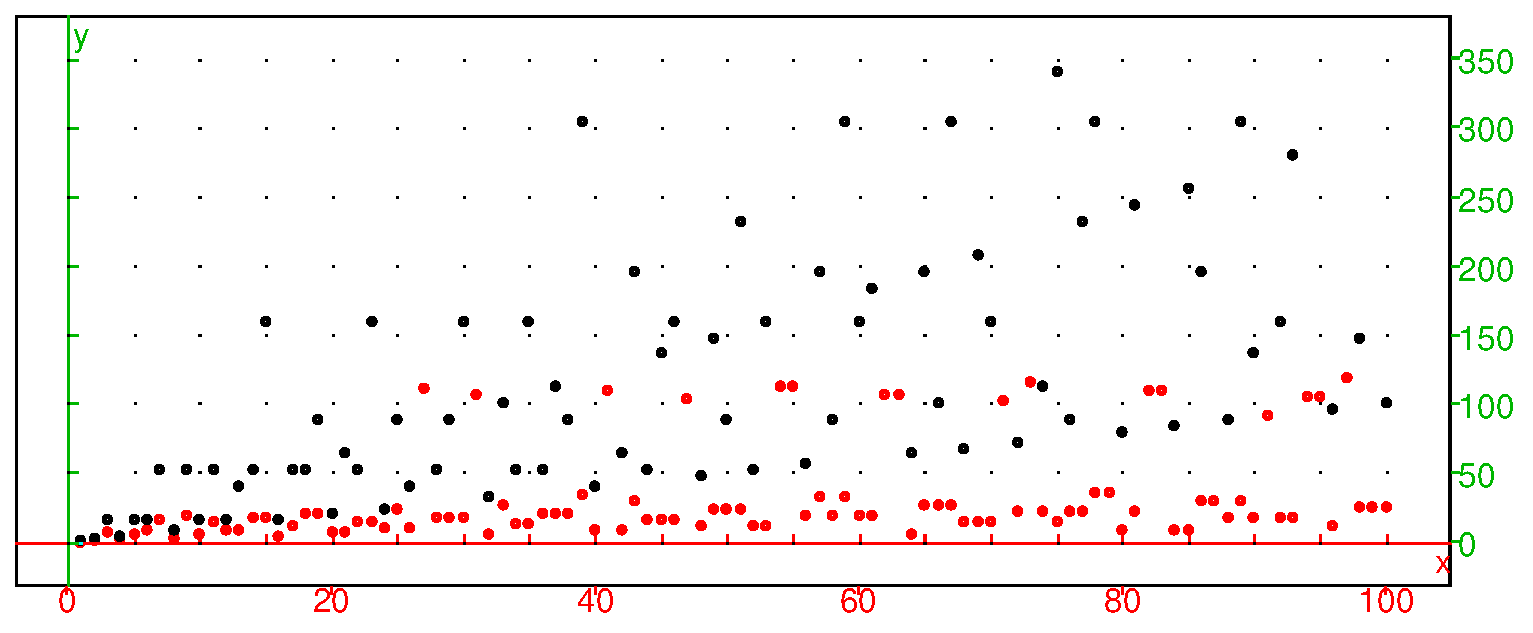
\includegraphics[width=\textwidth]{syracuse}
Mais en changeant le rep\`ere, on voit les points tels que point(97,9232)\\
\ \\
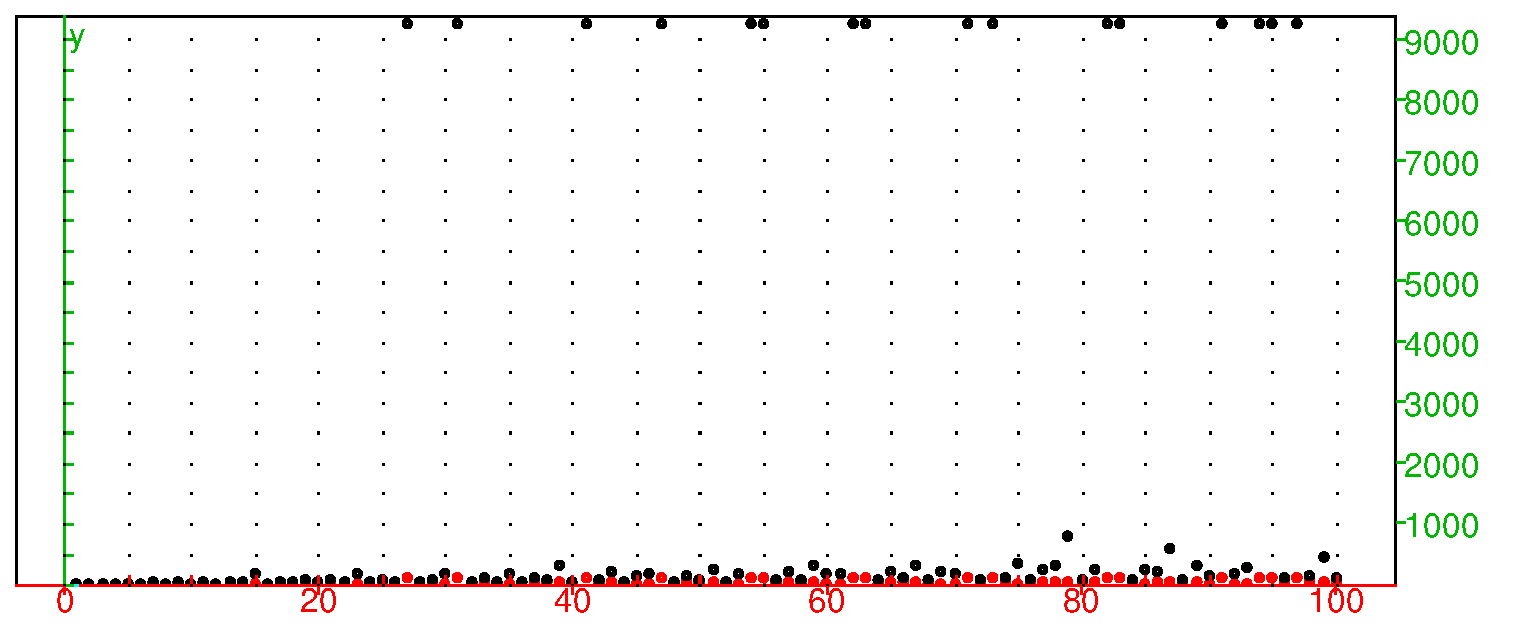
\includegraphics[width=\textwidth]{syracuse1}

\section{En 2009 Centre \'etranger}
On consid\`ere la fonction $f(x)=xe^x-1$ sur $\R$.
\begin{itemize}
\item Calculer $f(0$ et $f(1)$.
En \'etudiant les variations de $f$ sur $\R$, montrer que $f(x)=0$ 
admet une solution unique dans [0;1].
\item On consid\`ere l'algorithme :
\begin{verbatim}
Entrée :         f la fonction pr\'ec\'edente 
                 n un entier
Variables :      a,b,m,p
Initialisation : Affecter à a la valeur 0
                 Affecter à b la valeur 1 
Traitement :     Tant que b-a>10^-n faire
                   Affecter à m la valeur (a+b)/2
                   Affecter à p la valeur f(a)*f(m)
                   Si p>0 
                     Affecter à a la valeur m
                   Sinon
                     Affecter à b la valeur m
                   FinSi 
                 FinTantque
Sortie :         a,b
\end{verbatim}
On fait fonctionner cet algorithme avec $n=1$.\\
Donner les valeurs que prennent successivement les diff\'erents param\`etres. 
\item Que d\'etermine cet algorithme ? \\
Quel influence le nombre $n$ a-t-il sur le r\'esultat obtenu ?
\end{itemize}
\ \\
{\bf La solution}\\
On a $f(0)=-1$ et $f(1)\simeq 1.71828182846$\\
Sur $]-\infty;0]$ $f(x)=xe^x-1\leq -1<0$  donc $f$ ne s'annule pas.\\ 
La fonction $f$ est continue et est strictement croissante sur $[0;+\infty[$ 
puisque sa deriv\'ee  $f'(x)=e^x(x+1)$ est n\'egative sur $]-\infty;-1[$ et 
positive sur $]-1;+\infty[$.\\
Donc d'apr\`es le th\'eor\`eme des valeurs interm\'ediaires $f(x)=0$ a une 
solution unique comprise entre 0 et 1 puisque $f(0)<0$ et $f(1)>0$.\\
L'algorithme trouve un encadrement de longueur inf\'erieure \`a $1O^{-n}$ de 
cette solution : a chaque \'etape on partage l'intervalle $[a;b]$ en deux 
(dichotomie). Si $m$ est le milieu  de $[a;b]$, on regarde si $f(a)$ et $f(m)$ 
sont de m\^eme signe : si oui, $m$ peut remplacer $a$ et sinon $m$ peut 
remplacer $b$ et le z\'ero se trouve toujours entre $a$ et $b$.\\
Lorsque $n=1$ cet encadrement est de longueur $0,1$\\
{\bf Initialisation : } $a$=0 et $b$=1\\
{\bf Etape 1 : } $m$=0.5, $p=f(0)f(0.5)=0.17563936465$, $a$=0.5, $b$=1\\
{\bf Etape 2 : } $m$=0.75, $p=f(0.5)f(0.75)=-0.103232038761$, $a$=0.5, $b$=0.75\\
{\bf Etape 3 : } $m$=0.625, $p=f(0.5)f(0.625)=-0.02944659346$,$a$=0.5, $b$=0.625\\
{\bf Etape 4 : } $m$=0.5625, $p=f(0.5)f(0.5625)=0.002244979408$,$a$=0.5625, $b$=0.625\\
{\bf R\'esultat : } 0.5625,0.625\\
Arr\^et du tantque car ($b-a$)<0.1 et le r\'esultat est donc 0.5625,0.625.\\
\ \\
{\bf La traduction en langage {\tt Xcas}}
\begin{verbatim}
dichotomie(f,n):={
local a,b,m,p;
a:=0.;
b:=1.;
tantque b-a>10^-n faire
  m:=(a+b)/2;
  p:=f(a)*f(m);
  si p>0 alors 
    a:=m;
  sinon
    b:=m;
  fsi;
ftantque;
retourne a,b;
}:;
\end{verbatim}
On tape :
{\tt dichotomie(f,1)}\\
On obtient :
{\tt 0.5625,0.6250}\\
On tape :
{\tt dichotomie(f,2)}\\
On obtient :
{\tt 0.5625,0.5703125}\\
On tape :
{\tt dichotomie(f,5)}\\
On obtient :
{\tt 0.567138671875,0.56714630127}
{\bf Compl\'ements}
Dans la fonction {\tt dichotomie} si dessus on a supposé que la fonction 
{\tt f} avait un z\'ero sur ]0.0,1.0[. Voici une fonction {\tt dichotomie}
plus g\'en\'erale que je nomme  {\tt dichotom}
\begin{verbatim}
dichotom(f,a,b,n):={
  local m,p;
  a:=evalf(a);b:=evalf(b);
  si a>b alors m:=b;b:=a;a:=m; fsi;
  p:=f(b)*f(a);
  si p>0 alors return("f(",a,")*f(",b,")>0"); fsi;
  DIGITS:=n+2;
  tantque (b-a)>10.0^-n faire 
    m:=(a+b)/2;
    p:=f(a)*f(m);
    si p>0 alors
      a:=m;
    sinon
      b:=m;
    fsi;
  ftantque ;
  retourne a,b;
}:;
\end{verbatim}
On tape :\\
{\tt f(x):=x*exp(x)-1;}
{\tt dichotom(f,0,1,15)}
On obtient :\\
{\tt 0.56714329040978351}\\
On tape :\\
{\tt dichotom(f,2,1,5)}
On obtient :\\
{\tt "f(",1.0,")*f(",2.0,")>0"}
\section{En 2010 Am\'erique du sud}
\begin{itemize}
\item On consid\`ere l'algorithme :
\begin{verbatim}
Entrée :         n un entier
Variables :      u,S,j
Initialisation : Affecter à u la valeur 1
                 Affecter à S la valeur 1 
                 Affecter à j la valeur 0 
Traitement :     Tant que j<n faire
                   Affecter à u la valeur 2u+1-j
                   Affecter à S la valeur S+u
                   Affecter à j la valeur j+1
                 FinTantque
Sortie :         u,S
\end{verbatim}
Justifier que pour $n=3$, le r\'esultat de cet algorithme  est  11,21 
\item On consid\`ere les suites $u_nn$ et $S_n$ d\'efinies par :\\
$u_0=1$ et $u_{n+1}=2u_n+1-n$\\
$S_n=u_0+u_+...+u_n$.\\
Que repr\'esente les valeurs donn\'ees par cet algorithme ?
\item Le but de cette question est de trouver $u_n$  en fonction de $n$
Modifier l'algorithme pour qu'il renvoie aussi $u_n-n$.
Montrer que $u_n-n=2^n$
\item Calculer $1+2+...+n\ $ et $\ 1+2+2^2+...+2^n$. \\
En d\'eduire $S_n$ en fonction de $n$.
\end{itemize}
\ \\
{\bf La solution}\\
Pour $n=3$, on a :\\
{\bf Initialisation : } u=1, S=1, j=0\\
{\bf Etape 1 : } u=3, S=4, j=1\\
{\bf Etape 2 : } u=6, S=10, j=2\\
{\bf Etape 3 : } u=11, S=21, j=3\\
{\bf R\'esultat : } 11,21\\
Arr\^et du tantque car j>=3 et le r\'esultat est donc 11,21.\\
Dans le corps du tantque on calcule $u,S$ et $j$ et on a $u=u_j$ et $S=S_j$.\\
Lorsque $j=n$ le tantque s'arr\^ete et renvoie $u_n,S_n$.\\ 
\ \\
{\bf La traduction en langage {\tt Xcas}}
\begin{verbatim}
suiteserie(n):= {
local u,S,j;
u:=1;
S:=1;
j:=0;
tantque j<n faire
  u:=2u+1-j;
  S:=S+u;
  j:=j+1;
ftantque;
retourne u,S
}:;
\end{verbatim}
On veut trouver $u_n$ en fonction de $n$, on modifie l'algorithme pour qu'il 
renvoie aussi $u_n-n$, on modifie seulement la sortie en {\tt u,s-n,S}\\
Pour $n=0$, on a :\\
{\bf Initialisation : } u=1, S=1, j=0\\
{\bf R\'esultat : } 1,1,1\\
Pour $n=1$, on a :\\
{\bf Initialisation : } u=1, S=1, j=0\\
{\bf Etape 1 : } u=3, S=4, j=1\\
{\bf R\'esultat : } 3,2,4\\
Pour $n=2$, on a :\\
{\bf Initialisation : } u=1, S=1, j=0\\
{\bf Etape 1 : } u=3, S=4, j=1\\
{\bf Etape 2 : } u=6, S=10, j=2\\
{\bf R\'esultat : } 6,4,10\\
Pour $n=3$, on a :\\
{\bf Initialisation : } u=1, S=1, j=0\\
{\bf Etape 1 : } u=3, S=4, j=1\\
{\bf Etape 2 : } u=6, S=10, j=2\\
{\bf Etape 3 : } u=11, S=21, j=3\\
{\bf R\'esultat : } 11,8,21\\
Il semble que $u_n-n=2^n$.\\
On a en effet $u_{n+1}-(n+1)=2u_n+1-n-(n+1)=2(u_n-n)$.\\
On a $1+2+..+n=n(n+1)/2$ et $1+2+2^2+..+2^n=2^{n+1}-1$\\
Donc $S_n=n(n+1)/2+2^{n+1}-1$\\
On v\'erifie pour $n=3$ $u_3=2^3+3=8+3=11$ et $S_3=6+2^4-1=16+5=21$\\
On a bien $u_5=2^5+5=32+5=37$ et $S_5=5*3+64-1=78$\\
On tape :
{\tt suiteserie(3)}\hspace*{1cm}
On obtient :
{\tt 11,21}\\
On tape :
{\tt suiteserie(5)}\hspace*{1cm}
On obtient :
{\tt 37,78}\\
\ \\
{\bf Remarque}
Il me semble pr\'ef\'erable d'\'ecrire cet algorithme avec un {\tt pour}.\\
Mais attention !!! 
On doit utiliser la relation de r\'ecurrence sous la forme :\\
$u_n=2u_{n-1}+2-n$ ou bien $u_{n+1}=2u_n+2-(n+1)$ \\
car dans le corps du 
{\tt pour} on calcule successivement :\\$u_1,S_1$ lorsque $j=1$, $u_2,S_2$ 
lorsque $j=2$ et $u_n,S_n$ lorsque $j=n$.\\
Alors que pr\'ec\'edement avec {\tt tantque},
on utilise la relation $u_{n+1}=2u_n+1-n$ car on
calcule successivement $u_1,S_1$ lorsque $j=0$, $u_2,S_2$ 
lorsque $j=1$ et $u_n,S_n$ lorsque $j=n-1$ et c'est pourquoi la condition 
d'arr\^et du {\tt tantque} est {\tt j<n}.\\
On tape :
\begin{verbatim}
suiteserie1(n):= {
local u,S,j;
u:=1;
S:=1;
pour j de 1 jusque n faire
  u:=2u+2-j;
  S:=S+u;
fpour;
retourne u,u-n,S
}:;
\end{verbatim}
\section{En 2011 La R\'eunion}
On consid\`ere la fonction $f(x)=4e^{x/2}-5$ sur $\R$.\\
On note $C_f$ le graphe de  $f$ dans un rep\`ere orthogonal
\begin{itemize}
\item  Calculer $f(0)$ et $f(1)$.\\
En \'etudiant les variations de $f$ sur $\R$, montrer que $f(x)=0$ 
admet une solution unique dans [0;1].
\item On consid\`ere l'algorithme :
\begin{verbatim}
Entrée :         f la fonction precedente
                 p un réel >0
Variables :      a,b
Initialisation : Affecter à a la valeur 0
                 Affecter à b la valeur -1 
Traitement :     Tant que b<0 faire
                   Affecter à a la valeur a+p
                   Affecter à b la valeur f(a)
                 FinTantque
Sortie :         a-p,a
\end{verbatim}
Que fait cet algorithme ?\\
Que renvoie ce programme lorsque $p=1$ ? $p=0.1$ ? $p=0.01$ ? $p=0.001$ ?
\end{itemize}
{\bf La solution et traduction en langage {\tt Xcas}}\\
On a $f(0)=-1$ et $f(1)\simeq 1.5948850828$\\
La fonction $f$ est continue et est strictement croissante sur $\R$ puisque sa 
deriv\'e qui vaut $f'(x)=2e^{x/2}$ est positive.\\
Donc d'apr\`es le th\'eor\`eme des valeurs interm\'ediaires $f(x)=0$ a une 
solution unique comprise entre 0 et 1 puisque $f(0)<0$ et $f(1)>0$.\\
L'algorithme trouve un encadrement de longueur $p$ de cette solution.\\
Lorsque $p=1$ cet encadrement est $0,1$\\
Lorsque $p=0.1$ cet encadrement est $0.4,0.5$ car $f(0.4)\simeq -0.114388967359$<0 et $f(0.5)\simeq 0.136101666751$>0\\
Lorsque $p=0.1$ cet encadrement est $0.44,0.45$ car $f(0.44)\simeq -0.0156930776507$<0 et $f(0.45)\simeq 0.00929086476731$>0\\
Avec {\tt Xcas}, on tape pour d\'efinir la fonction $f$ :\\
{\tt f(x):=4*exp(x/2)-5)}\\
On tape la traduction de l'algorithme avec {\tt Xcas} :
\begin{verbatim}
zeroapprox(f,p):={
local a,b;
a:=0;
b:=f(a);
tantque b<0 faire 
  a:=a+p;
  b:=f(a);
ftantque;
retourne a-p,a
}:;
\end{verbatim}
On tape :
{\tt zeroapprox(f,0.1)}\\
On obtient :
{\tt 0.4,0.5}\\
On tape :
{\tt zeroapprox(f,0.01)}\\
On obtient :
{\tt 0.44,0.45}\\
On tape :
{\tt zeroapprox(f,0.001)}\\
On obtient :
{\tt 0.445999999998,0.446999999998}\\
On tape :
{\tt zeroapprox(f,0.0001)}\\
On obtient :
{\tt 0.446199999974,0.446299999974}\\
On remarquera que cet algorithme est 
valable pour toutes les fonctions continues $f$ qui v\'erifient
$f(0)<0$ et $f(1)>0$.\\ 
{\bf Remarque} 
Ce programme est moins performant que le programme de dichotomie vu 
pr\'ec\'edemment.

\section{En 2012 France}
Soit $(u_n )$ la suite définie pour tout entier strictement positif par :
$$u_n = 1 +\frac{1}{2}+\frac{1}{3}...+\frac{1}{n}-\ln(n)$$
\begin{enumerate}
\item On consid\`ere l’algorithme suivant :
\begin{verbatim}
Entrée :         l'entier n
Variables :      j  est un entier
                 u est un réel
Initialisation : Affecter à u la valeur 0
Traitement :     Pour j variant de 1 à n
                   Affecter à u la valeur u +1/j
                 fPour
Sortie :        Afficher u
\end{verbatim}
Donner la valeur exacte affich\'ee par cet algorithme lorsque l’utilisateur 
entre la valeur $n=3$.
\item Recopier et compl\'eter l’algorithme pr\'ec\'edent afin qu’il affiche la 
valeur de $u_n$ lorsque l’utilisateur entre la valeur de $n$.
\item Voici les r\'esultats fournis par l’algorithme modifi\'e, arrondis à 
$10^{-3}$.\\
\begin{tabular}{|c|c|c|c|c|c|c|c|c|c|}
\hline
$n$&6&7&8&9&10&100&1000&1500&2000\\
\hline
$u_n$&0.658&0.647&0.638&0.632&0.626&0.582&0.578&0.578&0.577\\
\hline
\end{tabular}
\`A l’aide de ce tableau, formuler des conjectures sur le sens de variation de 
la suite $(u_n)$ et son \'eventuelle convergence.
\end{enumerate}
\ \\
{\bf La solution et la traduction avec {\tt Xcas}}\\
Le but de l'exercice est de trouver une approximation de la constante 
d'Euler :\\
$\gamma=\lim_{n \rightarrow +\infty}(1+\frac{1}{2}+\frac{1}{3}...+\frac{1}{n}-\ln(n))$.\\
On montre dans un premier temps que cette limite existe car :\\
$u_n$ est d\'ecroissante en effet 
$\displaystyle u_{n+1}-u_n=\frac{1}{n+1}+\ln(\frac{n}{n+1})<0$  et\\
l'\'etude de $\displaystyle f(x)=\frac{1}{x+1}+\ln(\frac{x}{x+1})$ montre que 
$f$ est n\'egative sur $[1;+\infty[$.\\
de plus $u_n$ est minor\'ee par 0. En effet pour $p\in \N^*$,on a :\\
$\displaystyle\int_{x=p}^{x=p+1}\frac{dx}{x}=\ln(p+1)-\ln(p)<\frac{1}{p}$\\
En sommant cette in\'egalit\'e pour $p=1..n$ on a :\\
$\displaystyle\ln(n+1)<1+\frac{1}{2}+\frac{1}{3}...+\frac{1}{n}$ donc\\
$\displaystyle0<\ln(1+1/n)<1+\frac{1}{2}+\frac{1}{3}...+\frac{1}{n-1}+\frac{1}{n}-\ln(n)$\\
Ainsi $u_n$ est d\'ecroissante et minor\'ee par 0 elle a donc une limite 
positive appel\'ee "constante d'Euler".\\
{\bf L'algorithme} calcule $1+\frac{1}{2}+\frac{1}{3}...+\frac{1}{n}$\\
Pour $n=3$\\
{\bf Initialisation : } u=0\\
{\bf Etape 1 : } j=1, u=1\\
{\bf Etape 2 : } j=2, u=3/2\\
{\bf Etape 3 : } j=3, u=11/6\\
{\bf Resultat : } 11/6 ou 1.83333333333\\
On modifie l'algorithme pour qu'il affiche la suite $\displaystyle u_n=1+\frac{1}{2}+...+\frac{1}{n}-\ln(n)$, pour cela, il suffit de modifier la sortie :
\begin{verbatim}
Entrée :         l'entier n
Variables :      j et n sont des entiers naturels
                 u est un réel
Initialisation : Affecter à u la valeur 0
Traitement :     Pour j variant de 1 à n
                   Affecter à u la valeur u +1/j
                 fPour
Sortie :        Afficher u-ln(n)
\end{verbatim}
{\bf La traduction avec {\tt Xcas}}\\
On retourne une valeur num\'erique gr\^ace \`a {\tt evalf(u)} qui transforme le
rationnel $u$ en un nombre d\'ecimal. 
\begin{verbatim}
csteuler(n):={
local j, u;
u:=0;
pour j de 1 jusque n faire
  u:=u+1/j;
fpour;
retourne evalf(u)-ln(n);
}:;
\end{verbatim}
On tape :
{\tt csteuler(10)}\\
On obtient :
{\tt 0.626383160974}\\
On tape :
{\tt csteuler(100)}\\
On obtient :
{\tt 0.582207331651}\\
On tape :
{\tt csteuler(1000)}\\
On obtient :
{\tt 0.577715581568}\\
On tape :
{\tt csteuler(2000)}\\
On obtient :
{\tt 0.577465644068}\\
On tape :
{\tt csteuler(20000)}\\
On obtient :
{\tt 0.577240664693}\\
Cela montre que la constante d'Euler est proche de 0.577240664693.\\
On tape car {\tt Xcas} connait cette constante :\\
{\tt evalf(euler\_gamma)}\\
On obtient :\\
{\tt 0.5772156649018}\\
{\bf Remarque}
Les deux variantes de {\tt csteuler} \'ecrites ci-dessous font \`a chaque 
\'etape un calcul num\'erique car on a mis {\tt 1./j} au lieu de {\tt 1/j}.
{\tt csteuler0} calcule la somme des $\frac{1}{k}$ pour $k$ allant de 1 \`a $n$, alors que
{\tt csteuler1} calcule la somme des $\frac{1}{k}$ pour $k$ allant de $n$ \`a 1
\begin{verbatim}
csteuler0(n):={
local j, u;
u:=0;
pour j de 1 jusque n faire
  u:=u+1./j;
fpour;
retourne u-ln(n);
}
:;
csteuler1(n):={
local j, u;
u:=0;
pour j de n jusque 1 pas -1 faire
  u:=u+1./j;
fpour;
retourne u-ln(n);
}:;
\end{verbatim}
On tape :
{\tt csteuler0(2000)}\\
On obtient :
{\tt 0.577465643831}\\
On tape :
{\tt csteuler1(2000)}\\
On obtient :
{\tt 0.577465644032}\\
On tape :
{\tt csteuler(2000)}\\
On obtient :
{\tt 0.577465644068}\\
Il faut comprendre la diff\'erence des r\'esultats obtenus entre les 
fonctions {\tt csteuler0}, {\tt csteuler1} et {\tt csteuler} :\\
{\tt csteuler1} donne un r\'esultat meilleur que {\tt csteuler0} car il 
commence par ajouter des petits nombres donc la somme conserve plus de  
d\'ecimales.\\
Le r\'esultat de {\tt csteuler} est encore meilleur car il ne fait 
l'approximation d\'ecimale qu'\`a la fin du programme.
\section{D'autres algorithmes sur ce mod\`ele}
\subsection{Calcul de 1+2+..+$n^2$}
Soit la suite $u_n=1+4+..+n^2$.\\
\'Ecrire un algorithme qui calcule $u_n$ en fonction de $n$.\\
Puis calculer successivement $u_n/n$ et $u_n/(n(n+1))$ pour $n=1..10$\\
Montrer que $\displaystyle u_n=\frac{n(n+1)(2n+1)}{6}$\\
{\bf La solution}\\
On \'ecrit l’algorithme :
\begin{verbatim}
Entrée :         l'entier n
Variables :      j est un entier
                 S est un réel
Initialisation : Affecter à S la valeur 0
Traitement :     Pour j variant de 1 à n
                   Affecter à S la valeur S+j^2
                 fPour
Sortie :        Afficher S
\end{verbatim}
{\bf Avec {\tt Xcas}} :
\begin{verbatim}
Scarre(n):={
local j,S;
S:=0;
pour j de 1 jusque n faire
  S:=S+j^2;
fpour
retourne S;
}:;
\end{verbatim}
On tape :
{\tt Scarre(p)\$(p=0..10)}\\
On obtient :\\
{\tt 0,1,5,14,30,55,91,140,204,285,385}\\
On tape :
{\tt (Scarre(p)/p)\$(p=0..10)}\\
On obtient :\\
{\tt 1,5/2,14/3,15/2,11,91/6,20,51/2,95/3,77/2}\\
On tape :
{\tt (Scarre(p)/(p*(p+1)))\$(p=1..10)}\\
On obtient :\\
{\tt 1/2,5/6,7/6,3/2,11/6,13/6,5/2,17/6,19/6,7/2}\\
On tape :
{\tt ((2p+1)/6)\$(p=1..10)} et
on obtient le r\'esultat pr\'ec\'edent.\\
Il reste donc \`a d\'emontrer par r\'ecurrence que :\\
$\displaystyle u_n=1+2^2+..+n^2=\frac{n(n+1)(2n+1)}{6}$
\subsection{Calcul de 1+1/4+..+1/$n^2$}
\'Ecrire un algorithme qui calcule $u_n=1+1/4+..+1/n^2$ en fonction de $n$.\\
{\bf La solution :} on \'ecrit l’algorithme :
\begin{verbatim}
Entrée :         l'entier n>=1
Variables :      j un entier, S un réel
Initialisation : Affecter à S la valeur 0
Traitement :     Pour j variant de 1 à n
                   Affecter à S la valeur S+1/j^2
                 fPour
Sortie :        Afficher S
\end{verbatim}
{\bf Avec {\tt Xcas}}
\begin{verbatim}
Scarre(n):={
local j,S;
S:=0;
pour j de 1 jusque n faire
  S:=S+1/j^2;
fpour
retourne S;
}:;
\end{verbatim}
On tape :
{\tt Sinvcarre(p)\$(p=1..9)}\\
On obtient :
{\tt 1,5/4,49/36,205/144,5269/3600,5369/3600,\\266681/176400,1077749/705600,9778141/6350400}\\
On tape :
{\tt evalf(Sinvcarre(p))\$(p=0..9)}\\
On obtient  :
{\tt 1.0,1.25,1.36111111111,1.42361111111,1.46361111111,\\
1.49138888889,1.51179705215,1.52742205215,1.53976773117,}\\
On tape (on admet que $u_n$ tend vers $\pi^2/6$ quand $n$ tend vers $+\infty$) :\\
{\tt sqrt(6.*Sinvcarre(1000))}\\
On obtient :
{\tt 3.14063805621}
\subsection{Calcul des termes de la suite de Fibonacci}
 La suite de Fibonacci $u_n$ est d\'efinie par :\\
$u_0=1,\ u_1=1,\ u_{n+2}=u_{n+1}+u_n$ pour $n\in \N$\\
\'Ecrire un algorithme qui calcule $u_n$ en fonction de $n$.\\
{\bf La solution :} on \'ecrit l’algorithme :
\begin{verbatim}
Entrée :         l'entier n.
Variables :      j,a,b,c sont des entiers
Initialisation : Affecter à a la valeur 1
                 Affecter à b la valeur 1
Traitement :     Pour j variant de 2 à n
                   Affecter à c la valeur a+b
                   Affecter à a la valeur b
                   Affecter à b la valeur c
                 fPour
Sortie :         Afficher b
\end{verbatim}
{\bf Avec {\tt Xcas}}
\begin{verbatim}
fibo(n):={
local j,a,b,c;
a:=1;
b:=1;
pour j de 2 jusque n faire
  c:=a+b;
  a:=b;
  b:=c;
fpour;
retourne b;
}:;
\end{verbatim}
On tape :\\
{\tt fibo(p)\$(p=0..10)}\\
On obtient les 11 premiers termes de la suite de Fibonacci :\\
{\tt 1,1,2,3,5,8,13,21,34,55,89}\\
On tape :\\
{\tt fibo(101)/fibo(100)}\\
On obtient :\\
{\tt 927372692193078999176/573147844013817084101}\\
On tape :\\
{\tt evalf(fibo(101)/fibo(100)),(1+sqrt(5))/2.}\\
On obtient :\\
{\tt 1.61803398875, 1.61803398875}\\
Il reste \`a montrer que $\displaystyle v_n=\frac{u_{n+1}}{u_n}$ tend vers \`a 
$\displaystyle \frac{1+\sqrt 5}{2}$ qui est le nombre d'or.
\chapter{Des programmes tres simples sur les cha\^{\i}nes de caract\`eres}
\section{Compter un nombre d'occurences}
\subsection{Nombre d'occurences d'une lettre}
On parcourt la cha\^{\i}ne $S$ et on augmente le compteur $n$ de 1 lorsqu'il y a 
\'egalit\'e avec le caract\`ere $c$.
\begin{verbatim}
Occurc(c,S):={
  local n,d,j;
  d:=dim(S)-1;
  n:=0;
  pour j de 0 jusque d faire
    si c==S[j]  alors n:=n+1 fsi;
  fpour;
  retourne n;
}:;
\end{verbatim}
On tape :\\
{\tt Occurc("e","occurrences")}\\
On obtient : {\tt 2}
\subsection{Nombre d'occurences d'une sous-cha\^{\i}ne}
Il faut comparer \`a chaque \'etape la sous-cha\^{\i}ne  {\tt ch} avec un morceau de
la cha\^{\i}ne  {\tt S} qui a m\^eme longueur.\\
On va utiliser {\tt mid(S,j,k)} qui renvoie la sous cha\^{\i}ne de  {\tt S} de
longueur {\tt k} qui commence \`a l'indice  {\tt j} ou {\tt mid(S,j)} qui 
renvoie la sous-cha\^{\i}ne fin de  {\tt S} commen\c{c}ant \`a l'indice  {\tt j}.\\
{\bf Remarque} \`A la place de {\tt mid(S,j,k)} on peut aussi utiliser 
{\tt S[j..j+k-1]} (on met les indices de d\'ebut et de fin de la sous-cha\^{\i}ne) 
et \`a la place de {\tt mid(S,j)} on peut aussi utiliser {\tt S[j..dim(S)-1]}.\\
On consid\`ere que dans "aaa" on voit une seule sous-cha\^{\i}ne "aa".
\begin{verbatim}
Occurch(ch,S):={
  local n,d,j,k;
  d:=dim(S)-1;
  k:=dim(ch);
  n:=0;
  j:=0;
  tantque j<= d-k+1 faire
    si ch==mid(S,j,k)  alors 
      n:=n+1; 
      j:=j+k; 
      sinon
        j:=j+1
    fsi;
  fpour;
  retourne n;
}:;
\end{verbatim}
On tape :\\
{\tt Occurch("e","occurrences")}\\
On obtient : {\tt 2}\\
On tape :\\
{\tt Occurch("az","aaazaaazaaaz")}\\
On obtient : {\tt 3}\\
On tape :\\
{\tt Occurch("aa","aaazaaazaaaz")}\\
On obtient : {\tt 3}

\section{Supprimer une lettre et sous-cha\^{\i}ne}
\subsection{Supprimer une lettre}
On parcourt la cha\^ine $S$  lorsqu'il y a 
\'egalit\'e avec le caract\`ere $c$ il faudra supprimer ce caract\`ere en 
faisant une concat\'enation entre ce qu'il y a avant $c$ (si $c$ est d'indice 
$j$ c'est {\tt mid(S,0,j)} car ce qu'il y a avant $c$ est de longueur $j$) et 
ce qu'il y a apr\`es $c$ ({\tt mid(S,j+1)}). On met alors \`a jour la longueur 
de $S$.
\begin{verbatim}
Supprimec(c,S):={
  local d,j;
  d:=dim(S)-1;
  j:=0;
  tantque j<=d faire
    si c==S[j]  alors 
      S:=mid(S,0,j)+mid(S,j+1);
      d:=d-1;
    sinon
      j:=j+1
    fsi;
  ftantque;
  retourne S;
}:;
\end{verbatim}
On tape :\\
{\tt Supprimec("e","occurrences")}\\
On obtient : {\tt "occurrncs"}
\subsection{Supprimer une sous-cha\^{\i}ne}
On parcourt la cha\^{\i}ne $s$  lorsqu'il y a 
\'egalit\'e avec la sous-cha\^{\i}ne $ch$ il faudra supprimer cette sous-cha\^{\i}ne en 
faisant une concat\'enation entre ce qu'il y a avant $ch$ et ce qu'il y a 
apr\`es $ch$. On met alors \`a jour la longueur de $S$.
\begin{verbatim}
Supprimech(ch,S):={
  local k,d,j;
  d:=dim(S)-1;
  k:=dim(ch);
  j:=0;
  tantque j<=d faire
    si ch==mid(S,j,k)  alors 
      S:=mid(S,0,j)+mid(S,j+k);
      d:=d-k;
    sinon
      j:=j+1
    fsi;
  ftantque;
  retourne S;
}:;
\end{verbatim}
On tape :\\
{\tt Supprimech("e","occurrences")}\\
On obtient : {\tt "occurrncs"}\\
On tape :\\
{\tt Supprimech("az","azerazerazaz")}\\
On obtient : {\tt "erer"}\\
On tape :\\
{\tt Supprimesch("aa","aaazaaazaaaz")}\\
On obtient : {\tt "azazaz"}

\section{Remplacer une lettre ou une sous-cha\^{\i}ne par une autre cha\^{\i}ne}
\subsection{Remplacer une lettre par une autre lettre}
Pour remplacer le caract\'ere $a$ par $b$ dans $S$, on parcourt $S$ et quand 
on trouve le caract\'ere $a$ on change ce caract\'ere.
\begin{verbatim}
Remplaceab(a,b,S):={
local d,j;
  d:=dim(S)-1;
  j:=0;
  tantque j<=d faire
    si a==S[j]  alors 
      S:=mid(S,0,j)+b+mid(S,j+1);
    sinon
      j:=j+1
    fsi;
  ftantque;
  retourne S;
}:;
\end{verbatim}
On tape :\\
{\tt Remplaceab("a","e","azerazerazaz")}\\
On obtient : {\tt "ezerezerezez"}
\subsection{Remplacer une sous-cha\^{\i}ne par une autre}
Pour remplacer la sous-cha\^{\i}ne $cha$ par la sous-cha\^{\i}ne $chb$ dans $S$, on 
parcourt $S$ et quand on trouve la sous-cha\^{\i}ne $cha$. on 
fait une concat\'enation entre ce qu'il y a avant $cha$, la sous-cha\^{\i}ne $chb$
et ce qu'il y a apr\`es $cha$. On met alors \`a jour la longueur de $S$.
\begin{verbatim}
Remplacechab(cha,chb,S):={
local ka,kb,d,j;
  d:=dim(S)-1;
  ka:=dim(cha);
  kb:=dim(chb);
  j:=0;
  tantque j<=d faire
    si cha==mid(S,j,ka)  alors 
      S:=mid(S,0,j)+chb+mid(S,j+ka);
      d:=d-ka+kb;
    sinon
      j:=j+1
    fsi;
  ftantque;
  retourne S;
}:;
\end{verbatim}
On tape :\\
{\tt Remplacechab("a","e","azerazerazaz")}\\
On obtient : {\tt "ezerezerezez"}\\
On tape :\\
{\tt Remplacechab("az","bcd","azerazerazaz")}\\
On obtient : {\tt "bcderbcderbcdbcd"}


\chapter{Des programmes tres simples pour les Math\'ematiques}
\section{D\'efinir le minimum}
\subsection{Minimum de 2 nombres}
Pour trouver le minimum de $a$ et $b$ et on compare $a$ et $b$.
Le minimum vaut $a$ si $a<=b$ et sinon il vaut $b$.\\
On remarquera que puisque l'instruction {\tt retourne} fait sortir du programme,
on peut \'ecrire le programme sans utiliser de {\tt sinon}. 
\begin{verbatim}
Mini(a,b):={
  si a<=b alors retourne a;fsi;
  retourne b;
}:;
\end{verbatim}
On tape :\\
{\tt Mini(23,4*6)}\\
On obtient : {\tt 23}\\
On tape :\\
{\tt Mini(1.5,sqrt(2))}\\
On obtient : {\tt sqrt(2)}

\subsection{Minimum de 3 nombres}
On utilise le fait que :\\
Min($a,b,c$)=Min(Min($a,b),c$)\\
et on utilise le programme pr\'ec\'edent.
\begin{verbatim}
Mini3(a,b,c):={
  local m;
  m:=Mini(a,b);
  m:=Mini(m,c);
  retourne m;
}:;
\end{verbatim}
On tape :\\
{\tt Mini3(3\verb|^|3,4*6,5\verb|^|2)}\\
On obtient : {\tt 24}\\
On tape :\\
{\tt Mini3(1.5,sqrt(2),1.41)}\\
On obtient : {\tt 1.41}

\subsection{Minimum d'une liste de nombres}
Pour trouver le minimum de la liste $L$, on parcourt la liste $L$ en utilisant
une variable $m$ qui sera le minimum de ce que l'on vient de parcourir et qui 
sera mis \`a jour au fur et \`a mesure que l'on parcourt la liste $L$.\\
On renvoie $m$ et l'indice $jm$ qu'il a dans $L$.
\begin{verbatim}
MiniL(L):={
  local m,j,d,a,jm;
  d:=dim(L)-1;
  m:=L[0];
  jm:=0;
  pour j de 1 jusque d faire
    a:=L[j];
    si a<m alors 
      m:=a;
      jm:=j;
    fsi;
  fpour;
  retourne m,jm;
}:;
\end{verbatim}
On tape :\\
{\tt MiniL([12,32,3,23,5,2,45])}\\
On obtient : {\tt 2}\\
\section{Trier}
\subsection{Ordonner 2 nombres par ordre croissant}
\begin{verbatim}
Trier(a,b):={
  si a<=b alors retourne a,b;fsi;
  retourne b,a;
}:;
\end{verbatim}
On tape :\\
{\tt Trier(125/3,163/4)}\\
On obtient : {\tt 163/4,125/3}\\
\subsection{Ordonner 3 nombres par ordre croissant}
\begin{verbatim}
Trier3(a,b,c):={
  si a>b alors a,b:=b,a;fsi;
  si c<=a alors retourne c,a,b;fsi;
  si c<=b alors retourne a,c,b; fsi;
  retourne a,b,c;
}:;
\end{verbatim}
On tape :\\
{\tt Trier3(12,1,23)}\\
On obtient : {\tt 1,12,23}
\subsection{Ordonner une s\'equence de nombres par ordre croissant}
\subsubsection{Tri par recherche du minimum}
On utilise une liste $Lrep$ pour mettre la liste tri\'ee.
On parcourt la liste $L$ pour chercher l'indice $jm$ du plus 
petit \'el\'ement $m$, puis on le met dans la liste $Lrep$ et et on enl\`eve 
cet \'el\'ement de $L$ on enl\`eve cet \'el\'ement de $L$
Puis on refait la m\^eme chose avec la liste priv\'ee de son premier 
\'el\'ement etc..\\
On va utiliser {\tt mid(L,j,k)} qui renvoie la sous liste de {\tt L} de
longueur {\tt k} qui commence \`a l'indice {\tt j} ou {\tt mid(S,j)} qui 
renvoie la liste fin de {\tt L}  commen\c{c}ant \`a l'indice {\tt j} .\\
{\bf Remarque} \`A la place de {\tt mid(L,j,k)} on peut aussi utiliser 
{\tt L[j..j+k-1]} (on met les indices de d\'ebut et de fin de la sous liste) et
\`a la place de {\tt mid(L,j)} on peut aussi utiliser 
{\tt L[j..dim(L)-1]}.\\
\begin{verbatim}
TrierLr(L):={
  local j,k,m,jm,d,Lrep;
  d:=dim(L)-1;
  Lrep:=[];
  pour j de 0 jusque d faire 
    m,jm:=MiniL(L);
    Lrep:=append(Lrep,m);
    L:=concat(mid(L,0,jm),mid(L,jm+1));
  fpour
 retourne Lrep;
}:;
\end{verbatim}
On utilise la m\^eme liste $L$ pour mettre la liste tri\'ee.
On parcourt la liste $L$ pour chercher l'indice $jm$ du plus 
petit \'el\'ement $m$, puis on l'\'echange avec le premier \'el\'emment de $L$.
Puis on refait la m\^eme chose avec la liste priv\'ee de son premier 
\'el\'ement etc...C'est le tri par recherche du minimum.
\begin{verbatim}
TrierL(L):={
  local j,k,m,jm,d;
  d:=dim(L)-1;
  pour k de 0 jusque d-1 faire
    jm:=k;
    m:=L[k];
    pour j de k+1 jusque d faire
      si m>L[j] alors m:=L[j];jm:=j; fsi;
    fpour;
  L[jm]:=L[k];
  L[k]:=m;
  fpour
 retourne L;
}:;
\end{verbatim}
On tape :\\
{\tt TrierLr([23,12,1,14,21,4,45,11])}\\
Ou on tape :\\
{\tt TrierL([23,12,1,14,21,4,45,11])}\\
On obtient : {\tt [1,4,11,12,14,21,23,45]}\\
\subsubsection{Tri par insertion}
On utilise une liste la m\^eme lisre $L$ pour mettre la liste tri\'ee.
\`A chaque \'etape on ins\`ere l'\'el\'ement suivant {\tt a=L[k]} dans 
le d\'ebut de la liste qui est d\'ej\`a tri\'ee. Quand on a trouv\'e o\`u» il 
fallait ins\'erer $a$ par exemple entre {\tt L[j-1]} et {\tt L[j]} il faut lui 
faire de la place en d\'ecalant d'un cran vers la droite les \'el\'ements de 
{\tt L} de $j$ jusque $k$. C'est le tri par insertion.
\begin{verbatim}
TrieL(L):={
  local j,k,d,a,p;
  d:=dim(L)-1;
  pour k de 1 jusque d faire
    j:=0;
    a:=L[k];
    tantque a>L[j] faire j:=j+1; ftantque
    si j<k alors 
      // on d\'ecale d'un cran vers la droite
      pour p de k jusque j+1 pas -1 faire
        L[p]:=L[p-1]
      fpour;
      L[j]:=a;
    fsi
  fpour
  retourne L;
}:;
\end{verbatim}
On tape :\\
{\tt TrieL([23,12,1,14,21,4,45,11])}\\
On obtient : {\tt [1,4,11,12,14,21,23,45]}
\subsubsection{Tri par fusion}
\`A chaque \'etape on partage la liste $L$ en deux listes $L_1$ er $L_2$
de m\^eme longueur. On trie ces 2 listes gr\^ace \`a 2 appels r\'ecursifs, 
puis on les fusionnne. Pour cela on \'ecrit la fonction  {\tt fusion}
qui fusionne 2 listes tri\'ees : \`a chaque \'etape on compare un \'el\'ement
de $L_ 1$ avec un \'el\'ement de $L_2$, on met le plus petit des 2 dans la liste
r\'eponse et on avance l'indice correspondant au plus petit d'un cran et on 
recommence...\\
On tape :
\begin{verbatim}
fusion(L1,L2):={
local d1,d2,j1,j2,L;
 d1:=dim(L1)-1;
 d2:=dim(L2)-1;
 L:=[];
 j1:=0;
 j2:=0;
tantque j1<=d1 et j2<=d2 faire
 si L1[j1]<L2[j2] alors L:=append(L,L1[j1]); j1:=j1+1;
   sinon  L:=append(L,L2[j2]); j2:=j2+1;
 fsi;
ftantque;
si j1<=d1 alors L:=concat(L,mid(L1,j1);
 sinon   L:=concat(L,mid(L2,j2);
fsi;
retourne L;
}:;

Trifusion(L):={
  local d,d1,L1,L2;
  d:=dim(L);
  si d==1 ou d==0 alors retourne L;fsi;
  d1:=iquo(d,2);
  L1:=mid(L,0,d1);
  L2:=mid(L,d1);
  L1:=Trifusion(L1);
  L2:=Trifusion(L2);
  retourne fusion(L1,L2);
}:;
\end{verbatim}

On peut am\'eliorer le programme pr\'ec\'edent en utilisant une liste que l'on modifie
en place (avec l'op\'erateur \verb|=<|) afin de ne pas recopier la liste \verb|L|
\`a chaque affectation par \verb|:=|. 
Attention, cela n\'ecessite de faire
une copie de la liste vide initiale par \verb|copy| 
sinon c'est la liste du programme
lui-m\^eme qui sera modifi\'ee et ne sera donc plus initialis\'ee \`a une liste vide.
\begin{verbatim}
fusionenplace(L1,L2):={
local d1,d2,j1,j2,k,j,L;
 d1:=dim(L1)-1;
 d2:=dim(L2)-1;
 L:=copy([]);
 j1:=0;
 j2:=0;
 k:=0;
 tantque j1<=d1 et j2<=d2 faire
   si L1[j1]<L2[j2] alors L[k]=<L1[j1]; j1:=j1+1;
   sinon  L[k]=<L2[j2]; j2:=j2+1;
   fsi;
   k:=k+1;
 ftantque;
 pour j de j1 jusque d1 faire
   L[k]=<L1[j];
   k:=k+1;
 fpour;
 pour j de j2 jusque d2 faire
   L[k]=<L2[j];
   k:=k+1;
 fpour;
 retourne L;
}
:;
Trifusionenplace(L):={
  local L1,L2,d1,d;
  d:=dim(L);
  si d==1 ou d==0 alors retourne L;fsi;
  d1:=iquo(d,2);
  L1:=mid(L,0,d1);
  L2:=mid(L,d1);
  L1:=Trifusionenplace(L1);
  L2:=Trifusionenplace(L2);
  retourne fusionenplace(L1,L2);
}
:;
\end{verbatim}
\section{D\'efinir une fonction par morceaux}
On peut utiliser l'instruction {\tt si...sinon} ou l'instruction {\tt ifte} ou 
mieux l'instruction {\tt when} (ou avec la version infix\'ee de {\tt when} qui 
est {\tt ?}).\\
 Soit la fonction $f$ d\'efinie par :\\
$$f(x)=\left\{
\begin{array}{rl}
 -1& \mbox{si }x<0\\
 0& \mbox{si  }x=0\\
 +1& \mbox{si  }x>0
\end{array}
\right.
$$
On tape
\begin{verbatim}
 f(x):={
  si x<0 alors retourne -1;fsi;
  si x==0  alors retourne 0 fsi;
  si x>0 alors retourne 1;fsi;
}:;
\end{verbatim}
mais on peut aussi \'ecrire la m\^eme chose avec l'instruction {\tt ifte} :\\
 {\tt f(x):=ifte(x<0,1,ifte(x==0,0,1)}\\
Mais il faut alors savoir que pour que  {\tt f(a)} soit valable il faut que 
{\tt a} contienne une valeur.\\
Par contre si on tape :\\
{\tt g(x):=when(x<0,1,when(x==0,0,1)}\\
ou\\
{\tt g(x):=(x>0)? 1 : ((x==0)? 0 : -1)}\\
{\tt g(a)} est valable m\^eme si {\tt a} est symbolique i.e. ne contient pas
de valeur.
\section{Convertir}
\subsection{Des secondes en jours, heures, minutes et secondes}
On se donne un nombre $ns$ de secondes que l'on veut convertir en heures $h$, 
minutes $mn$ et secondes $s$. On a : $$ns=3600h+60mn+s=s+60(mn+60h)$$
On tape :
\begin{verbatim}
converth(ns):={
  local h,mn,s;
  s:=irem(ns,60);
  ns:=iquo(ns,60);
  mn:=irem(ns,60);
  h:=iquo(ns,60);
retourne h,mn,s;
}:;
\end{verbatim}
On tape :\\
{\tt converth(123456789)}\\
On obtient : {\tt 34293,33,9}\\
Si on veut aussi convertir en jours $j$, heures $h$, 
minutes $mn$ et secondes $s$. On a : 
$$ns=24*3600j+3600h+60mn+s=s+60(mn+60(h+24j))$$
Ou bien, on tape :
\begin{verbatim}
convertj(ns):={
  local j,h,mn,s;
  s:=irem(ns,60);
  ns:=iquo(ns,60);
  mn:=irem(ns,60);
  ns:=iquo(ns,60);
  h:=irem(ns,24);
  j:=iquo(ns,24);
retourne j,h,mn,s;
}:;
\end{verbatim}
On tape :\\
{\tt convertj(123456789)}\\
On obtient : {\tt 1428,21,33,9}

\subsection{Des degr\'es en radians}
Si la mesure d'un angle est $rad$  en radians et $deg$ en degr\'es, on a :
$$rad=deg*\pi/180$$
\begin{verbatim}
deg2rad(deg):=deg*pi/180;
\end{verbatim}
On tape :\\
{\tt deg2rad(48.2384062423)}\\
On obtient : {\tt 0.841919014843}
\subsection{Des radians en degr\'es}
Si la mesure d'un angle est $rad$  en radians et $deg$ en degr\'es, on a :
$$deg=rad*180/\pi$$
\begin{verbatim}
rad2deg(rad):=rad*180/pi;
\end{verbatim}
On tape :\\
{\tt rad2deg(0.841919014843)}\\
On obtient : {\tt 48.2384062423}

\section{Les fractions}
\subsection{Simplifier une fraction}
On suppose que l'on donne la fraction $F$ sous la forme de la liste $[N,D]$ de 
son num\'erateur et de son d\'enominateur. Pour la simplifier il suffit de 
diviser le num\'erateur et le d\'enominateur par leur pgcd.\\
On utilise ici la fonction {\tt gcd} de {\tt Xcas} pour le calcul du pgcd.
On tape :
\begin{verbatim}
Simplifie(F):={
 local pgcd,N,D;
 N:=F[0];
 D:=F[1];
 pgcd:=gcd(N,D);
 retourne [N/pgcd,D/pgcd];
}:;  
\end{verbatim}
On tape :\\
{\tt Simplifie([5544,55]);}\\
On obtient : {\tt [504,5]}
\subsection{Additionner 2 fractions}
On commence par simplifier les 2 fractions, puis on cherche leur d\'enominateur
commun qui est le ppcm de leur d\'enominateurs, On r\'eduit ces fractions \`a 
ce d\'enominateur commun et on ajoute les num\'erateurs. \\
On suppose que l'on donne les fraction $F1$ et $F2$  sous la forme de la liste 
$[N,D]$. Puis on simplifie le r\'esultat.\\
On utilise ici la fonction {\tt lcm} de {\tt Xcas} pour le calcul du ppcm.
\begin{verbatim}
Ajoute(F1,F2):={
 local ppcm,N1,D1,N2,D2,N,D;
 F1:=Simplifie(F1);
 F2:=Simplifie(F2);
 N1:=F1[0];
 D1:=F1[1];
 N2:=F2[0];
 D2:=F2[1];
 D:=lcm(D1,D2);
 N1:=N1*D/D1;
 N2:=N2*D/D2;
 retourne Simplifie([N1+N2,D]);
}:;
\end{verbatim}
On tape :\\
{\tt Ajoute([1234,22],[5549,55])}\\
On obtient : {\tt [8634,55]}
\subsection{Multiplier 2 fractions}
On commence par simplifier les 2 fractions, puis on multiplie les num\'erateurs
entre eux et les d\'enominateurs entre eux. Puis on simplifie le r\'esultat.
\begin{verbatim}
Multiple(F1,F2):={
 local N1,D1,N2,D2;
 F1:=Simplifie(F1);
 F2:=Simplifie(F2);
 N1:=F1[0];
 D1:=F1[1];
 N2:=F2[0];
 D2:=F2[1];
 retourne Simplifie([N1*N2,D1*D2]);
}:;
\end{verbatim}
On tape :\\
{\tt Multiple([1234,22],[5549,55])}\\
On obtient : {\tt [3423733,605]}
\chapter{Des programmes  tres simples pour les Statistiques}
\section{Simulation du lancer d'une pi\`ece}
On veut tirer au hasard  0 ou 1 (par exemple 0=pile et 1=face).\\
On utilise la fonction {\tt rand(n)} qui renvoie un entier al\'eatoire 
uniform\'ement distribu\'e dans {\tt 0.. n-1}.\\ 
On tape :
\begin{verbatim}
tirage_piece():=rand(2);
\end{verbatim}
\section{Simulation d'un d\'e}
On veut tirer au hasard un nombre entier dans [1.. 6].\\
On utilise la fonction {\tt rand(n)} qui renvoie un entier al\'eatoire 
uniform\'ement distribu\'e dans {\tt 0.. n-1}.\\ 
On tape :
\begin{verbatim}
tirage_de():=1+rand(6);
\end{verbatim}
\section{Simulation d'une variable al\'eatoire}
On tire au hasard un nombre entier $n$ de [0,1,2,3].\\
On tire au hasard un nombre r\'eel $m$ de [0,1[.\\
On veut simuler une variable al\'eatoire $X$ qui vaut 
la partie enti\`ere de $m*n$.\\
On utilise la fonction {\tt rand(p,n)} qui renvoie un r\'eel al\'eatoire 
uniform\'ement distribu\'e dans {\tt [p.. n[}.\\ 
On tape :
\begin{verbatim}
X():={
local n;
n:=rand(4);
return floor(n*rand(0,1));
}
\end{verbatim}
Quelle est la fonction de r\'epartition de $X$ ?
$X$ vaut :\\
0 si (($n=0$ ou $n=1$) et $m \in [0,1[$) ou ($n=2$ et $m \in [0,0.5[$) ou 
($n=3$ et $m \in [0,1/3[$)\\
1 si ($n=2$ et $m \in [0.5,1[$) ou ($n=3$ et $m \in [1/3,2/3[$)\\
2 si $n=3$ et $m \in [2/3,1[$\\
On a donc :\\
Proba($X=0)$=1/4+1/4+1/4*1/2+1/4*1/3=17/24\\
Proba($X=1)$=1/4*1/2+1/4*1/3=5/24\\
Proba($X=2)$=1/4*1/3=1/12\\
On v\'erifie que l'on a :  17/24+5/24+1/12=1
\section{Simulation d'une variable al\'eatoire}
On tire au hasard un nombre entier $n$ de [1,2,3].\\
On veut simuler une variable al\'eatoire $Y$ qui vaut  $\sum_{j=1}^nj$.\\
On tape :
\begin{verbatim}
Y():={
local n,j,x;
n:=1+rand(3);
x:=0;
pour j de 1 jusque n faire
x:=x+j;
fpour;
return x;
}:;
\end{verbatim}
Quelle est la fonction de r\'epartition de $Y$ ?
$Y$ vaut :\\
1 si $n=1$\\
3 si $n=2$\\
6 si $n=3$\\
On a donc :\\
Proba($X=1)$)=1/3\\
Proba($X=3)$)=1/3\\
Proba($X=6)$)=1/3\\
On aurait pu aussi simuler cette loi en tapant :
\begin{verbatim}
Z():={
local n;
n:=rand(3);
si n==0 alors return 1 fsi;
return 3*n;
}:;
\end{verbatim}
\section{Comment simplifier $\sqrt{a+\sqrt{b}}\ $ lorsque $(a,b)\in \N^2$}
On veut \'ecrire $\sqrt{a+\sqrt{b}}$ sous la forme $\sqrt{x/2}+\sqrt{y/2}$ bien 
sur quand cela est possible.\\
Si $\sqrt{x/2}+\sqrt{y/2}=\sqrt{a+\sqrt{b}}$ on a :\\
$(\sqrt{x/2}+\sqrt{y/2})^2=a+\sqrt b=(x+y)/2+\sqrt{xy}$\\
d'o\`u $x+y=2a$ et $xy=b$\\
donc $x$ et $y$ sont solutions de l'\'equation $X^-2aX+b=0$\\
donc si $a^2-b$ est un carr\'e parfait i.e. $a^2-b=c^2$ avec $c$ entier on a :\\
$x=a+c$ et $y=a-c$\\
Donc si $a^2-b$ est un carr\'e parfait on a si $a^2-b=c^2$ :
$$\sqrt{a+\sqrt{b}}=\sqrt{\frac{a+c}{2}}+\sqrt{\frac{a-c}{2}}=\frac{\sqrt{2(a+c)}+\sqrt{2(a-c)}}{2}$$
On tape la fonction {\tt simply} qui doit avoir {\tt r=sqrt(a+sqrt(b))} comme 
param\`etre o\`u {\tt b} est sans facteur carr\'e :
\begin{verbatim}
simply(r):={
local f,a,b,c,d;
si sommet(r)=='^' alors
  f:=feuille(r);
  a,d:=feuille(f[0]);
  si type(a)==integer alors
  b:=feuille(d)[0];
  c:=sqrt(a^2-b);
  si (round(c))^2==a^2-b alors 
    retourne sqrt((a+c)/2)+sqrt((a-c)/2) 
  fsi;
  sinon 
  d,a:=feuille(f[0]);
  b:=feuille(d)[0];
  c:=sqrt(a^2-b);
  si (round(c))^2==a^2-b alors 
    retourne sqrt((a+c)/2)+sqrt((a-c)/2) 
  fsi;
  fsi;
fsi;
retourne r;
}:;
\end{verbatim}
On tape :\\
{\tt simply(sqrt(9+sqrt(17)))}\\
ou \\
{\tt simply(sqrt(sqrt(17)+9))}\\
On obtient :\\
{\tt (sqrt(34))/2+(sqrt(2))/2}
 on tape la fonction {\tt simplyf} qui doit avoir  comme param\`etre
{\tt r} de la forme {\tt sqrt(a+s*sqrt(b))} ou {\tt sqrt(a+sqrt(b))}:
\begin{verbatim}
simplyf(r):={
local f,a,b,c,d,s,sb;
si sommet(r)=='^' alors
  f:=feuille(r);
  a,d:=feuille(f[0]);
  si type(a)==integer alors
     f:=feuille(d);
    si f[1]==1/2 alors 
      s:=1;
      b:=f[0];
    sinon
      s,sb:=f;
      si type(s)==integer alors
        b:=feuille(sb)[0];
      sinon
       sb,s:=f;
       b:=feuille(sb)[0];
      fsi;
    fsi;
    c:=sqrt(a^2-s^2*b);
    si (round(c))^2==a^2-s^2*b alors 
      retourne sqrt((a+c)/2)+sqrt((a-c)/2); 
    fsi;
  sinon
    d,a:=feuille(f[0]);
    f:=feuille(d);
    si f[1]==1/2 alors 
      b:=f[0];
      s:=1;
    sinon
      s,sb:=f;
      si type(s)==integer alors
        b:=feuille(sb)[0];
      sinon
       sb,s:=f;
       b:=feuille(sb)[0];
      fsi;
    fsi;
    c:=sqrt(a^2-s^2*b);
    si (round(c))^2==a^2-s^2*b alors 
      retourne sqrt((a+c)/2)+sqrt((a-c)/2); 
    fsi;
  fsi;
fsi;
retourne r;
}:;
\end{verbatim}
On tape (car {\tt Xcas} remplace {\tt sqrt(128)} par {\tt 8*sqrt(2)} :\\
{\tt simplyf(sqrt(18+sqrt(128)))}\\
ou \\
{\tt simplyf(sqrt(sqrt(128)+18))}\\
ou \\
{\tt simplyf(sqrt(8*sqrt(2)+18))}\\
ou \\
{\tt simplyf(sqrt(18+8*sqrt(2)))}\\
ou \\
{\tt simplyf(sqrt(sqrt(2)*8+18))}\\
ou \\
{\tt simplyf(sqrt(18+sqrt(2)*8))}\\
On obtient :\\
{\tt 4+sqrt(2)}
On tape :\\
{\tt simplyf(sqrt(194320499737857776523212040+19713979797994*sqrt(97160249868928888261606031)))}\\
On obtient :\\
{\tt sqrt(97160249868928888261606031)+9856989898997}

\chapter{Les programmes d'arithm\'etique}
\section{Quotient et reste de la division euclidienne}
\subsection{Les fonctions iquo, irem et smod de {\tt Xcas}}\index{iquo}\index{irem}\index{smod}\index{mod}\index{\%}
Si $a$ et $b$ sont des entiers ou des entiers de Gauss :\\
{\tt iquo(a,b)} renvoie le quotient $q$ de la division euclidienne de $a$ par $b$ et\\
{\tt irem(a,b)} renvoie le reste $r$ de la division euclidienne de $a$ par $b$.\\
$q$ et $r$ v\'erifient :\\
si $a$ et $b$ sont entiers $a=b*q+r$ avec $0 \leq r<b$\\
si  $a$ et $b$ sont des entiers de Gauss $a=b*q+r$ avec $|r|^2) \leq \frac{|b|^2}{2}$. \\
Par exemple si $a=-2+6*i$ et si $b=1+3*i$ on a :\\
$q=2+i$ et  $r=-1-i$\\
Si $a$ et $b$ sont des entiers relatifs {\tt smod(a,b)} renvoie le reste 
sym\'etrique $rs$ de la division euclidienne de $a$ par $b$.\\
$q$ et $rs$ v\'erifient :\\
$a=b*q+rs$ avec $-\frac{b}{2}<rs \leq \frac{b}{2}$\\
Exemples :\\
{\tt smod(7,4)=-1}\\
{\tt smod(-10,4)=-2}\\
{\tt smod(10,4)=2}\\
{\bf Remarque}
{\tt mod} (ou {\tt \%}) est une fonction infix\'ee et d\'esigne un \'el\'ement 
de $Z/nZ$.\\
On a  : {\tt 7 mod 4=-1\%4} d\'esigne un \'el\'ement de $Z/4Z$ mais\\
{\tt smod(7,4)=(7\%4)\%0=-1} d\'esigne un entier.
\subsection{Activit\'e}
\subsubsection {le texte de l'exercice}
\begin{enumerate}
\item V\'erifier que : 
$$\frac{13}{18}=\frac{1}{2}+\frac{1}{5}+\frac{1}{45}$$
\item On donne deux entiers $a$ et $b$ v\'erifiant : $0<b <a$.
On note $q$ et $r$ le quotient et le reste de la division euclidienne de $a$ 
par $b$ ($a=bq+r$ avec $0\leq r<b$).

D\'emontrer que :
$$q>0$$
$$\frac{1}{q+1}<\frac{b}{a} \leq \frac{1}{q}$$
\item On d\'efinit $u$ et $v$ par :
$$\frac{b}{a}-\frac{1}{q+1}=\frac{v}{u}$$ et
$$u=a(q+1)$$
Exprimer $v$ en fonction de $b$ et $r$.

D\'emontrer que :
$$v\leq b<a<u$$
Si $r=0$, v\'erifier que : $$\frac{b}{a}=\frac{1}{q}$$
\item Si $r$ est diff\'erent de z\'ero, on pose :
$a_1=u$ et $b_1=v$.

Puis, on recommence :
on divise $a_1$ par $b_1$. \\
On trouve un quotient $q_1$ et un reste $r_1$.Si $r_1 $ est nul, v\'erifier 
que :
$$\frac{b}{a}=\frac{1}{q+1}+\frac{1}{q_1}$$
Si $r_1$ n'est pas nul, on recommence.

Montrer qu'il existe une suite finie d'entiers $Q_0, Q_1,...Q_n$ strictement 
croissante telle que :
$$\frac{b}{a}=\frac{1}{Q_0}+\frac{1}{Q_1}+...+\frac{1}{Q_n}$$
\item R\'ediger l'algorithme d\'ecrit ici et l'appliquer \`a la fraction : $$\frac {151}{221}$$
\end{enumerate}
\subsubsection{L'algorithme}
On suppose que la fraction ${\tt \displaystyle \frac{NUM}{DENOM}\in]0;1[}$.

L'algorithme s'\'ecrit en langage non fonctionnel :\\
{\tt
 \noindent DENOM $\rightarrow$A\\
NUM$\rightarrow$B\\
Quotient(A, B)$\rightarrow$Q\\
Reste(A, B)$\rightarrow$R\\
tantque R $\neq$0 faire \\
\indent Q+1$\rightarrow$D\\
\indent Afficher D\\
\indent B-R$\rightarrow$B\\
\indent A*D$\rightarrow$A\\
\indent Quotient(A, B)$\rightarrow$Q\\
\indent Reste(A, B)$\rightarrow$R\\
ftantque\\
Afficher Q\\}
\subsubsection{Traduction Xcas}
On \'ecrit la fonction {\tt decomp} qui va d\'ecomposer selon l'algorithme la 
fraction {\tt frac}. Cette fonction va renvoyer  la liste {\tt lres} \'egale 
\`a ${\tt [Q_0,..Q_n]}$ avec ${\tt 0<Q_0<,..<Q_n}$ et 
${\tt frac=1/Q_0+..+1/Q_n}$.\\
Attention {\tt frac=b/a} et donc {\tt fxnd(frac)=fxnd(b/a)=[b,a]}.
\begin{verbatim}
decomp(frac):={
local a,b,l,q,r,lres;
l:=fxnd(frac);
b:=l[0];
a:=l[1];
q:=iquo(a,b);
r:=irem(a,b);
lres:=[];
while (r!=0) {
lres:= concat(lres, q+1);
b:=b-r;
a:=a*(q+1);
q:=iquo(a,b);
r:=irem(a,b);
}
lres:=concat(lres,q);
return lres;
}
\end{verbatim}
\subsubsection{Application \`a $\frac{151}{221}$}
On tape :\\
{\tt decomp(151/221)}\\
On obtient :\\
{\tt [2,6,61,5056,40895962,4181199228867648]}\\
On v\'erifie :\\
{\tt 1/2+1/6+1/61+1/5056+1/40895962+1/4181199228867648}\\
On obtient :\\
{\tt 151/221}\\
On peut \'ecrire un programme pour faire le v\'erification :\\
{\tt size(l)} est \'egal \`a la longueur de la liste {\tt l}
\begin{verbatim}
verifie(l):={
local s,k,res;
s:=size(l);
res:=0;
for (k:=0;k<s;k++){
res:=res+1/l[k];
}
return res;
}
\end{verbatim}
On tape :\\
{\tt verifie([2,6,61,5056,40895962,4181199228867648])}\\
On obtient :\\
${\tt \frac{151}{221}}$

\section{Calcul du PGCD par l'algorithme d'Euclide}
Soient $A$ et $B$ deux entiers positifs dont on cherche le $PGCD$.\\
L'algorithme d'Euclide est bas\'e sur la d\'efinition r\'ecursive du $PGCD$ :
\begin{eqnarray*}
PGCD(A,0) & = & A \\
PGCD(A,B) & = & PGCD(B,A \ \bmod \  B) \  si \  B \neq 0
\end{eqnarray*}
o\`u $A\ \bmod \ B$ d\'esigne le reste de la division euclidienne de $A$ par $B$.\\
Voici la description de cet algorithme :\\
on effectue des divisions euclidiennes successives :
\begin{eqnarray*}
A=& B \times Q_1+R_1  &  0 \leq R_1 < B \\
B=& R_1 \times Q_2+R_2  & 0 \leq R_2 < R_1 \\
R_1=& R_2 \times Q_3+R_3 & 0 \leq R_3 < R_2 \\
.......
\end{eqnarray*}
Apr\`es un nombre fini d'\'etapes, il existe un entier n tel que : 
$R_n = 0.$ \\
on a alors :\\
$PGCD(A,B)= PGCD(B,R_1) =...$\\
$PGCD(R_{n-1},R_n) = PGCD(R_{n-1},0) = R_{n-1}$
\subsection{Traduction algorithmique}
-Version it\'erative\\
Si $B\neq  0$ on calcule $R=A \bmod B$, puis   avec $B$ dans le r\^ole 
de $A$ (en mettant  $B$ dans $A$ ) et $R$ dans le r\^ole de $B$ ( en mettant 
$R$ dans $B$) on recommence jusqu'\`a ce que $B=0$, le $PGCD$ est alors \'egal
\`a $A$.
\begin{verbatim}
fonction PGCD(A,B)
local R
\end{verbatim}
{\tt tantque B $\neq$ 0 faire}
\begin{verbatim}
  A mod B=>R
  B=>A
  R=>B
ftantque
retourne A
ffonction
\end{verbatim}

 -Version r\'ecursive\\
On \'ecrit simplement la d\'efinition r\'ecursive vue plus haut.
\begin{verbatim}
fonction PGCD(A,B)
\end{verbatim}
{\tt Si B $\neq$ 0 alors}
\begin{verbatim}
  retourne PGCD(B,A mod B) 
  sinon
  retourne A
fsi
ffonction
\end{verbatim}
\subsection{Traduction Xcas}
- Version it\'erative :
\begin{verbatim}
pgcd(a,b):={
  local r; 
  while (b!=0){
   r:=irem(a,b);
   a:=b;
   b:=r;
  } 
  return(a);
};
\end{verbatim}
- Version r\'ecursive.
\begin{verbatim}
pgcdr(a,b):={
  if (b==0) 
    return(a);
  else 
    return(pgcdr(b,irem(a,b)));
};
\end{verbatim}
\subsection{Traduction MapleV}
-Version it\'erative :
\begin{verbatim}
pgcd:=proc(x,y)
local a,b,r:
a:=x:
b:=y:
while (b>0) do
r:=irem(a,b):
a:=b:
b:=r:
od:
RETURN(a):
end:
\end{verbatim}

-Version r\'ecursive :
\begin{verbatim}
pgcd:=proc(a,b)
if (b=0) then
RETURN(a)
 else 
RETURN(pgcd(b,irem(a,b))):
fi:
end:
\end{verbatim}
\subsection{Traduction MuPAD}
-Version it\'erative :
\begin{verbatim}
pgcd:=proc(a,b)
local r:
begin
while (b>0) do
r:=a mod b:
a:=b:
b:=r:
end_while:
return(a):
end_proc;
\end{verbatim}

-Version r\'ecursive :
\begin{verbatim}
pgcd:=proc(a,b)
begin
if (b=0) then
 return(a)
 else 
return(pgcd(b,a mod b)):
end_if:
end_proc;
\end{verbatim}
\subsection{Traduction TI89 92}
-Version it\'erative
\begin{verbatim}
:pgcd(a,b)
:Func 
:Local r
\end{verbatim}
{\tt :While b $\neq$ 0 }
\begin{verbatim}
:mod(a,b)=>r
:b=>a
:r=>b
:EndWhile
:Return a
:EndFunc
\end{verbatim}

-Version r\'ecursive
\begin{verbatim}
:pgcd(a,b)
:Func 
\end{verbatim}
{\tt :If  b $\neq$ 0 Then}
\begin{verbatim}
:Return  pgcd(b, mod(a,b)) 
:Else
:Return a
:EndIf
:EndFunc
\end{verbatim}
\subsection{Le pgcd dans $\Z[i]$}
On rappelle que $\Z[i]=\{m+n*i,\ (m,n)\in \Z^2\}$.\\
Soient $a \in \Z[i]$ et $b \in \Z[i]-\{0\}$, alors on dit que le quotient $q$
de $a$ par $b$ est l'affixe du (ou des) point(s), le plus proche pour le 
module, du point d'affixe $a/b$.
\begin{itemize}
\item Montrer que $|q-a/b|^2 \leq 1/2$. En d\'eduire que $|a-bq|^2 \leq |b|^2/2$
et que l'algorithme d'Euclide se termine lorsqu'on prend $q$ comme quotient 
euclidien.
\item \'Ecrire un programme qui calcule le pgcd de 2 nombres de $\Z[i]$. On 
normalisera le r\'esultat (en  multipliant le r\'esultat par 1,-1,i ou -i)
pour que le pgcd soit un nombre de partie r\`eelle 
strictement positive et de partie imaginaire positive ou nulle.
\end{itemize}
On tape :
\begin{verbatim}
quotient(a,b):={
local q1,q2,c;
c:=normal(a/b);
q1:=re(c);
q2:=im(c);
return round(q1)+i*round(q2);
}:;
pgcdzi(a,b):={
local q,r;
tantque b!=0 faire
  q:=quotient(a,b);
  r:=a-b*q;
  a:=b;
  b:=r;
ftantque;
//on normalise
si re(a)<0 et im(a)<=0 alors retourne -a;fsi;
si im(a)<0 alors retourne i*a;fsi;
si re(a)<=0 alors retourne -i*a;fsi;
retourne a;
}:;
\end{verbatim}
On tape :\\
{\tt pgcdzi(3+i,3-i)}\\
On obtient :
{\tt 1+i}\\
On tape :\\
{\tt pgcdzi(7+i,-6+17*i)}\\
On obtient :
{\tt 3+4*i}
\subsection{Le pgcd dans $\Z[i\sqrt 2]$}
On rappelle que $\Z[i\sqrt 2]=\{m+i*n\sqrt 2,\ (m,n)\in \Z^2\}$.\\
Soient $a \in \Z[i\sqrt 2]$ et $b \in \Z[i\sqrt 2]-\{0\}$, alors on dit que le 
quotient $q$ de $a$ par $b$ est l'affixe du (ou des) point(s), le plus proche 
pour le module, du point d'affixe $a/b$.
On tape :
\begin{verbatim}
quorest(a,b):={
local q1,q2,q,r,c;
c:=normal(a/b);
q1:=normal(round(re(c)));
q2:=normal(round(im(c)/sqrt(2)));
q:= q1+i*q2*sqrt(2);
r:=simplify(a-b*q);
return q,r;
}:;
pgcdzis2(a,b):={
local r;
tantque b!=0 faire
  r:=quorest(a,b)[1];
  a:=b;
  b:=r;
ftantque;
//on normalise
si re(a)<0  alors retourne -a;fsi;
retourne a;
}:;
\end{verbatim}
On tape :\\
{\tt pgcdzis2(3+i*sqrt(2),3-i*sqrt(2))}\\
On obtient :
{\tt 1}\\
On tape :\\
{\tt pgcdzis2(4+5*i*sqrt(2),-2+3*i*sqrt(2))}\\
On obtient :
{\tt 2-(3*i)*sqrt(2)}

\section{Identit\'e de B\'ezout par l'algorithme d'Euclide}
 Dans ce paragraphe la fonction {\tt Bezout(A,B)} renvoie  la liste $\{U, V, PGCD(A,B)\}$
o\`u $U$ et $V$ v\'erifient :
$ A \times U + B \times V = PGCD(A,B)$ 
\subsection{Version it\'erative sans les listes}
L'algorithme d'Euclide permet aussi de trouver un couple $U$ et $V$ 
v\'erifiant:

$ A \times U + B \times V= PGCD(A,B) $

En effet, si on note $ A_0$ et$ B_0 $ les valeurs de $A$ et de $B$ du d\'ebut on a :
\begin{eqnarray*}
 A & =A_0 \times U+B_0 \times V \ \  \mbox{avec} \  U=1 \ et\  V=0 \\ 
 B & =A_0 \times W+B_0 \times X  \ \ \mbox{avec} \  W=0 \ et \  X=1 
\end{eqnarray*}

 Puis on fait \'evoluer $A,\ B,\ U,\ V,\ W,\ X$ de fa\c{c}on \`a ce que ces 
deux relations  soient toujours v\'erifi\'ees. Voici comment
$A,\ B,\ U,\ V,\ W,\ X$ \'evoluent :\\
- on pose :
$ A=B \times Q+R \ \ \  0 \leq R < B \ \ ( R = A \bmod \ B \ et \  Q = E(A / B )) $\\
- on \'ecrit alors :
\begin{eqnarray*}
R=A-B \times Q=A_0 \times (U-W \times Q)+B_0 \times (V-X \times Q)=A_0 \times S+B_0 \times T \\
\mbox{avec} \  S=U-W \times Q \  \mbox{et} \   T=V-X \times Q
\end{eqnarray*}
Il reste alors \`a recommencer avec $B$ dans le r\^ole de $A$ ({\tt B=>A\  W=>U \ X=>V}) et $R$ dans le r\^ole de $B$ ({\tt R=>B \ S=>W \ T=>X} ) d'o\`u l'algorithme:
\begin{verbatim}
fonction Bezout(A,B)
local U,V,W,X,S,T,Q,R
1=>U 0=>V 0=>W 1=>X
\end{verbatim}
{\tt tantque B $\neq$ 0 faire}
\begin{verbatim}
A mod B=>R 
E(A/B)=>Q
//R=A-B*Q
U-W*Q=>S
V-X*Q=>T
B=>A W=>U X=>V
R=>B S=>W T=>X
ftantque
retourne {U, V, A}
ffonction
\end{verbatim}
\subsection{Version it\'erative avec les listes}
On peut simplifier l'\'ecriture de l'algorithme ci-dessus en utilisant moins de
 variables : pour cela on utilise les listes $LA$, $LB$, $LR$ pour m\'emoriser 
les triplets $\{U,\ V,\ A\}$,  $\{W,\ X,\ B\}$ et $\{S,\ T,\ R\}$.
Ceci est tr\`es commode car les logiciels de calcul savent ajouter des listes 
de m\^eme longueur (en ajoutant les \'el\'ements de m\^eme indice) et savent 
aussi multiplier une liste par un nombre (en multipliant chacun des 
\'el\'ements de la liste par ce nombre).\\
\begin{verbatim}
fonction Bezout(A,B)
local LA LB LR
{1, 0, A}=>LA
{0, 1, B}=>LB
\end{verbatim}
{\tt tantque LB[3] $\neq$ 0 faire}
\begin{verbatim}
LA-LB*E(LA[3]/LB[3])=>LR 
LB=>LA 
LR=>LB 
ftantque
retourne LA
ffonction
\end{verbatim}
\subsection{Version r\'ecursive sans les listes}\label{sec:recsl}
Si on utilise des variables globales pour {\tt A, B, D, U, V, T}, on peut voir 
la fonction {\tt Bezout} comme calculant \`a partir de {\tt A B}, des valeurs 
qu'elle met dans {\tt U, V, D (AU+BV=D)},  gr\^ace \`a une variable locale 
{\tt Q}.\\
On \'ecrit donc une fonction sans param\`etre : seule la variable {\tt Q} doit \^etre locale \`a la foncton alors que les autres variables {\tt A, B ...} 
sont  globales.\\
{\tt  Bezout} fabrique {\tt U, V, D}  v\'erifiant  {\tt A*U+B*V=D} \`a partir de {\tt A} et {\tt B}.
Avant l'appel r\'ecursif (on pr\'es\'erve {\tt E(A/B)=Q} et on  met {\tt A} et 
{\tt B} \`a jour ( nouvelles valeurs), apr\`es l'appel les variables  {\tt U, V, D}  v\'erifient 
 {\tt A*U+B*V=D} (avec {\tt A} et {\tt B} les nouvelles valeurs), il suffit 
alors de revenir aux premi\`eres valeurs de
{\tt A} et {\tt B} en \'ecrivant :\\   
{\tt B*U+(A-B*Q)*V=A*V+B*(U-V*Q)}  \\
On \'ecrit alors :
\begin{verbatim}
fonction Bezout
local Q 
Si B != 0 faire
E(A/B)=>Q
A-B*Q=>R
B=>A
R=>B
Bezout
U-V*Q=>W
V=>U
W=>V
sinon 
1=>U
0=>V
A=>D
fsi
ffonction
\end{verbatim}
\subsection{Version r\'ecursive avec les listes}
On peut d\'efinir r\'ecursivement la fonction Bezout par:

$ Bezout(A,0)=\{1,\ 0,\ A\} $  
   
Si $ B \neq 0 $ il faut d\'efinir $ Bezout(A,B)$ en fonction de $ Bezout(B,R)$ 
lorsque $ R=A-B \times Q$ et  $Q=E(A/B).$

On a:
\begin{eqnarray*} Bezout(B,R)=LT=\{W, X, pgcd(B,R)\} \\
\mbox{avec}\  W \times B+X \times R=pgcd(B,R)
\end{eqnarray*}
Donc:
\begin{eqnarray*}
 W \times B+X \times (A-B \times Q) & = & pgcd(B,R) \  \mbox{ou  encore} \\ 
X \times A+(W-X \times Q) \times B & = & pgcd(A,B).
\end{eqnarray*}
D'o\`u si $B \neq 0$ et si $ Bezout(B,R)=LT$  on a :

$ Bezout(A,B)=\{LT[2],\ LT[1]-LT[2] \times Q,\ LT[3]\}.$

\begin{verbatim}
fonction Bezout(A,B)
local LT Q R
\end{verbatim}
{\tt Si B $\neq$ 0 faire}
\begin{verbatim}
E(A/B)=>Q
A-B*Q=>R
Bezout(B,R)=>LT
retourne {LT[2], LT[1]-LT[2]*Q, LT[3]}
sinon retourne {1, 0, A} 
fsi
ffonction
\end{verbatim}
\subsection{Traduction Xcas}\label{sec:bezout}
- Version it\'erative avec les listes
\begin{verbatim}
bezout(a,b):={
//renvoie [u,v,d] tels que a*u+b*v=pgcd(a,b) (fct iterative)
local la,lb,lr,q,lb2;
la:=[1,0,eval(a)];
lb:=[0,1,eval(b)];
lb2:=eval(b);
while (lb2 !=0){
q:=iquo(la[2],lb2);
lr:=la+(-q)*lb;
la:=lb;
lb:=lr;
lb2:=lb[2];
}
return(la);
};
\end{verbatim}
- Version r\'ecursive avec les listes
\begin{verbatim}
bezoutr(a,b):={
//renvoie [u,v,d] tels que a*u+b*v=pgcd(a,b) (fct recursive)
local lb,q,r;
if (b!=0) {
q:=iquo(a,b);
r:=irem(a,b);
lb:=bezoutr(b,r);
return([lb[1],lb[0]+(-q)*lb[1],lb[2]]);
} else 
return([1,0,a]);
};
\end{verbatim}

\section{D\'ecomposition en facteurs premiers d'un entier}
Dans cette section, on ne suppose pas connue une table de nombres premiers : 
on ne se sert donc pas du programme crible.
\subsection{Les algorithmes et leurs traductions algorithmiques}
\begin{itemize}
\item Premier algorithme\\
Soit $N$ un entier.\\
On teste, pour tous les nombres $D$ de 2 \`a $N$, la divisibilit\'e de $N$ par 
$D$.\\
Si $D$ divise $N$, on cherche alors les diviseurs de $N/D$ etc...$N/D$ joue le 
r\^ole de $N$ et on s'arr\^ete quand $N=1$ \\
On met les diviseurs trouv\'es dans la liste {\tt FACT}.

\begin{verbatim}
fonction factprem(N)
local D FACT 
2 => D
{} => FACT
tantque N<= 1 faire
si N mod D = 0 alors
   concat(FACT,D) => FACT
    N/D => N
   sinon
    D+1 => D
 fsi
ftantque
retourne FACT
ffonction
\end{verbatim}

\item  Premi\`ere am\'elioration\\
On ne teste que les diviseurs $D$ entre 2 et $E(\sqrt N)$.\\
En effet si $N=D1*D2$ alors on a :\\
soit $D1 \leq E(\sqrt N)$, soit $D2 \leq E(\sqrt N)$ car sinon on aurait :\\
$D1*D2 \geq  (E(\sqrt N)+1)^2 >N$.

\begin{verbatim}
fonction factprem1(N)
local D FACT
2 => D
{} => FACT
tantque D*D!= N faire
si N mod D = 0 alors
    concat(FACT,D) => FACT
    N/D=> N
   sinon
    D+1 => D
 fsi
ftantque
concat(FACT,N) => FACT
retourne FACT
ffonction
\end{verbatim}
Dans la liste {\tt FACT}, on a les  diviseurs premiers \'eventuellement 
plusieurs fois, par exemple :\\
{\tt factprem1(12)=\{2,2,3\}}.
\item  Deuxi\`eme am\'elioration\\
On cherche si 2 divise $N$, puis on teste les diviseurs impairs $D$ entre 3 et 
$E(\sqrt N)$.
 
Dans la liste {\tt FACT}, on fait suivre chaque diviseur premier par son 
exposant, par exemple :\\
{\tt factprem2(12)=\{2,2,3,1\}}.
\begin{verbatim}
fonction  facprem2(N)
local K D FACT
{}=>FACT
0 => K
tantque N mod 2 == 0 faire
    K+1 => K
    N/2 => N
ftantque
si K !=0 alors
    concat(FACT,{2 K}) => FACT
fsi
3 =>D
tantque D*D<= N faire
    0 => K
    tantque N mod D = 0 faire
      K+1 => K
      N/D => N
    ftantque
    si K !=0 alors
      concat(FACT,{D K})=> FACT
    fsi
     D+2 => D
ftantque
si N != 1 alors
    concat(FACT,{N 1})=> FACT
fsi
retourne FACT
ffonction
\end{verbatim}
\item  Troisi\`eme am\'elioration\\
On cherche si 2 et 3 divisent $N$, puis on teste les diviseurs $D$ entre 5 et 
$E(\sqrt N)$ de la forme $6*k-1$ ou $6*k+1$.\\
On remarque que si :\\
 $D=6*k-1$ on a  $D+(4*D \bmod 6)= 6*k+1$\\
 et que si :\\
 $D=6*k+1$ on a  $D+(4*D \bmod 6)=6*(k+1)-1$\\
Dans la liste {\tt FACT}, on fait suivre  chaque diviseur par son exposant,
 par exemple :\\
{\tt factprem3(12)=\{2,2,3,1\}}.
\begin{verbatim}
fonction  factprem3(N)
local J,D,FACT 
2=>D
{}=>FACT
tantque (D*D<=N) faire
 0=>J
 tantque (N mod D=0) faire
   N/D=>N
   J+1=>J
 ftantque
si (J!= 0) alors concat(FACT,{D,J})=>FACT fsi
 si (D<4) alors 
   2*D-1=>D
 sinon
   D+(4*D mod 6)=>D
 fsi
ftantque
si (N !=1) alors concat(FACT,{N,1})=>FACT fsi
retourne(FACT)
ffonction
\end{verbatim} 
\end{itemize}
\subsection{Traduction Xcas}\label{sec:factprem}
On traduit la troisi\`eme am\'elioration.
\begin{verbatim}
factprem(n):={
//decompose n en facteur premier dans la liste l de dimension s
local j,d,s,l;
d:=2;
s:=0;
l:=[];
while (d*d<=n) {
j:=0;
while (irem(n,d)==0){
n:=iquo(n,d);
j:=j+1;
}
if (j!=0) {
l:=concat(l,[d,j]);
s:=s+2;
}
if (d<4) {
d:=2*d-1;
}
else {
d:=d+irem(4*d,6);
}
}
if (n!=1) {
l:=concat(l,[n,1]);
s:=s+2;
}
return([l,s]);
};
\end{verbatim}
\section{D\'ecomposition en facteurs premiers en utilisant le crible}
Pour effectuer la d\'ecomposition en facteurs premiers de $n$, on utilise la 
table des nombres premiers fabriqu\'ee par le crible : on ne teste ainsi que 
des nombres premiers.\\
Si on peut \'ecrire $N=A*D^J$ avec $PGCD(A,D)=1$  et $J>0$ alors  $D^J$ est un 
facteur de la d\'ecomposition de $N$.\\
On \'ecrit tout d'abord la fonction {\tt ddiv(N,D)} qui renvoie :\\
-  soit la liste :\\
{\tt [ N,[]]} si $D$ n'est pas un diviseur de $N$,\\
- soit la liste :\\
{\tt [A,[D,J]]} si $N=A*D^J$ avec $PGCD(A,D)=1$ et $J>0$.\\
 $D^J$ est alors un diviseur de $N$ et $A=N/D^J$ . 
\subsection{Traduction Algorithmique}
\begin{verbatim}
fonction ddiv(N,D)
//ddiv renvoie [a,[d,j]] (n=a*d^j, pgcd(a,d)=1) si j!=0 sinon [n,[]] 
local L,J
0=>J
tantque  (N mod D)=0) faire
N/D=>N
J+1=>J
ftantque
si (J=0) alors
{N,{}}=>L
sinon
{N,{D,J}}=>L
fsi
retourne(L)
ffonction
\end{verbatim}
On cherche la liste des nombres premiers plus petit que $\sqrt N$ et on met 
cette liste dans la variable $PREM$. Lorsque $N$>1, on teste si ces nombres 
premiers sont des diviseurs de $N$ en utilisant {\tt ddiv}. 
\begin{verbatim}
fonction criblefact(N)
//decomposition en facteurs premiers de n 
//en utilisant ddiv et crible
local D,PREM,S,LD,LDIV;
PREM:=crible(floor(sqrt(N)));
S:=dim(PREM);
LDIV:={};
1=>K
tantque (K<=S et N>1) faire 
  ddiv(N,PREM[K])=>LD
  concat(LDIV,ld[2])=>LDIV;
  LD[1]=>N
  K+1=>K
ftantque
si (N != 1) alors
 concat(LDIV,[N,1])=>LDIV;
fsi
retourne(LDIV);
}
\end{verbatim}
\subsection{Traduction Xcas}\label{sec:criblefact}
\begin{verbatim}
ddiv(n,d):={
//ddiv renvoie [a,[d,j]] (n=a*d^j, pgcd(a,d)=1) si j!=0 
//sinon [n,[]] 
local l,j;
j:=0;
while (irem(n,d)==0){
n:=iquo(n,d);
j:=j+1;
}
if (j==0){
l:=[n,[]];
} else {
l:=[n,[d,j]];
}
return(l);
}
\end{verbatim}
\begin{verbatim}
criblefact(n):={
//decomposition en facteurs premiers de n 
//en utilisant ddiv et crible
local d,prem,s,ld,ldiv;
prem:=crible(floor(sqrt(n)));
s:=size(prem);
ldiv:=[];
for (k:=0;k<s;k++){
ld:=ddiv(n,prem[k]);
ldiv:=concat(ldiv,ld[1]);
n:=ld[0];
k:=k+1;
}
if (n!=1){
ldiv:=concat(ldiv,[n,1]);
}
return(ldiv);
}
\end{verbatim}

\section{La liste des diviseurs}
\subsection{Les programmes avec les \'el\`eves}
L'algorithme na\"{i}f :\\
{\tt \noindent pour j de 1 a n faire\\
\hspace*{0.5cm} si (j divise n) alors\\
\hspace*{1cm} afficher j\\
\hspace*{0.5cm} fsi\\
fpour}\\

Les \'el\`eves remarquent que l'on peut avoir les diviseurs deux par deux.\\
{\tt \noindent pour j de 1 a E($\sqrt{\mbox{n}}$) faire\\
\hspace*{0.5cm} si (j divise n) alors\\
\hspace*{1cm} afficher j, n/j \\
\hspace*{0.5cm} fsi\\
fpour}\\
Malheureusement, lorsque l'entier $n$ est le carr\'e de $p$, $p$ figure deux 
fois dans l'affichage des diviseurs.\\
On am\'eliore donc l'algorithme :\\
 
{\tt \noindent 1  $\rightarrow$ j\\
tantque j<$\sqrt{\mbox{n}}$ faire\\
\hspace*{0.5cm} si (j divise n) alors\\
\hspace*{1cm} afficher j, n/j \\
\hspace*{0.5cm} fsi\\
\hspace*{0.5cm} j+1 $\rightarrow$ j\\
ftantque\\
si j$\cdot$j=n alors\\
\hspace*{0.5cm} afficher j\\
fsi}
{\bf Remarque}
Les programmes sont ensuite mis sur des calculatrices, c'est pourquoi les 
algorithmes pr\'ec\'edents utilisent la commande {\tt afficher}. Si on veut 
\'ecrire un programme avec {\tt Xcas} on fera une fonction : on mettera les 
diviseurs dans une liste qui sera \`a la fin la valeur de la fonction en  
utilisant la commande {\tt retourne} par exemple :
\subsubsection{Traduction Xcas de l'algorithme na\"{i}f}
\begin{verbatim}
nbdivis(n):={
local j, L,sn;
L:=[];
j:=1;
sn:=sqrt(n)
tantque j<sn faire
si irem(n,j)==0 alors L:=concat(L,[j,n/j]); fsi;
j:=j+1;
ftantque;
si j*j==n alors L:=append(L,j) fsi;
retourne L;
}:;
\end{verbatim}

\subsection{Le nombre de diviseurs d'un entier $n$}
On d\'ecompose $n$ en facteurs premiers, puis on donne aux exposants de ces 
facteurs premiers toutes les valeurs possibles. 
Si $n=a^\alpha*b^\beta*c^\gamma$
l'exposant de $a$ paut prendre $\alpha+1$ valeurs (0..$\alpha$), celui de $b$
peut prendre $\beta+1$ valeurs et celui de $c$
peut prendre $\gamma+1$ valeurs donc le nombre de diviseurs de $n$ est $(\alpha+1)*(\beta+1)*(\gamma+1)$.
\subsection{L'algorithme sur un exemple} 
D\'escription de l'algorithme sur un exemple :\\
$n=360=2^3*3^2*5$\\
$n$ a donc (3+1)*(2+1)*(1+1)=24 diviseurs.\\
On les \'ecrit en faisant varier le triplet repr\'esentant les exposants avec 
l'ordre :\\ (0,0,0),(1,0,0),(2,0,0),(3,0,0),\\
(0,1,0),(1,1,0),(2,1,0),(3,1,0),\\
(0,2,0),(1,2,0),...,\\
(0,2,1),(1,2,1),(2,2,1),(3,2,1))\\
On a  $(a_1,\beta,\gamma) < (b_1,b_2,b_3)$ si :\\
$\gamma<b_3$ ou \\
$\gamma=b_3$ et $\beta<b_2$ ou \\
$\gamma=b_3$ et $\beta=b_2$  et $a_1<b_1$.\\
On obtient les 4*3*2=24 diviseurs de 360 :\\
1,2,4,8,3,6,12,24,9,18,36,72,5,10,20,40,15,30,60,120,45,90,180,360.\\
que l'on peut \'ecrire en le tableau suivant :\\
1,2,4,8 (les puissances de 2) \\
3,6,12,24 (3*les puissances de 2)\\
9,18,36,72 (3*3*les puissances de 2)\\
5,10,20,40 (5*les puissances de 2)\\
15,30,60,120 (5*3*les puissances de 2)\\
45,90,180,360 (5*3*3*les puissances de 2).\\
Comment obtient-on la liste des diviseurs de $a^\alpha*b^\beta*c^\gamma$ 
\`a partir de la liste {\tt L1} des diviseurs de $a^\alpha*b^\beta$ ?\\
Il suffit de rajouter \`a {\tt L1} la liste {\tt L2} constitu\'ee par :\\
${\tt c*L1,...,c^\gamma*L1}$\\
Dans le programme cette liste de diviseurs ({\tt L1}) sera donc constitu\'ee 
au fur et \`a mesure au moyen d'une liste ({\tt L2}) qui correspond au parcours
 de l'arbre.\\
On initialise {\tt L1} avec {\tt \{1\}}, puis on rajoute \`a {\tt L1}
la liste {\tt L2} form\'ee par :\\
${\tt a*L1,...,a^\alpha*L1}$.\\
Puis on recommence avec le diviseur suivant :\\ 
on rajoute \`a {\tt L1}
la liste {\tt L2} form\'ee par ${\tt b*L1,...,b^\beta*L1}$ etc...
\subsection{Les algorithmes donnant la liste des diviseurs de n } 
La liste {\tt L1} est la liste destin\'ee \`a contenir les diviseurs de {\tt N}.\\
Au d\`ebut  ${\tt L1=\{1\}}$ et ${\tt L2=\{\}}$.\\
Pour avoir la liste des diviseurs de {\tt N}, on cherche {\tt A} le premier 
diviseur de {\tt N} et on cherche {\tt a} la puissance avec quelle {\tt A}
 divise  {\tt N}.\\
On d\'efinit la liste {\tt L2} :\\
{\tt L2} est obtenue en concat\'enant, les listes {\tt L1*A}, ${\tt L1*A^2}$,
...,${\tt L1*A^a}$ : au d\'ebut {\tt L1=\{1\}} donc 
${\tt L2=\{A,A^2,...,A^a\}}$.\\
On modifie la liste {\tt L1} en lui concat\'enant la liste {\tt L2}, ainsi 
${\tt L1=\{1,A,A^2,...,A^a\}}$.\\
Puis, on vide la liste {\tt L2}. On cherche {\tt B} le deuxi\`eme  diviseur 
\'eventuel de {\tt N} et on 
cherche {\tt b} la puissance  avec quelle {\tt B} divise  {\tt N}.\\
On d\'efinit la nouvelle liste {\tt L2} :\\
{\tt L2} est obtenue en concat\'enant, les listes  {\tt L1*B}, ${\tt L1*B^2}$,
...,  ${\tt L1*B^b}$ (c'est \`a dire 
${\tt L2=\{B,B*A,B*A^2,..,B*A^aB^2,B^2*A,B^2*A^2,..,B^2*A^a,..,B^b*A^a,\}}$) \\
On modifie la liste {\tt L1} en lui concat\'enant la liste {\tt L2}, ainsi :\\
${\tt L1=\{1,A,A^2,...,A^a,B,B*A,B*A^2,...,B*A^a,...,B^b,B^b*A,B^b*A^2,...,B^b*A^a\}}$.\\
Et ainsi de suite, jusqu'\`a avoir epuis\'e tous les diviseurs de {\tt N}.
\subsubsection{Traduction Algorithmique}
\noindent{\tt fonction NDIV0(N)\\
local D,L1,L2,K}\\
${\tt 2 => D}$\\
${\tt \{1\} => L1}$\\
${\tt tant que \ (N \neq 1)\ faire}$\\
{\tt \{\}=>L2 }\\
${\tt 0=> K}$:\\
{\tt tantque ((N MOD D) =0) faire}\\
${\tt N/D=> N}$\\
${\tt K+1 =>K}$\\
${\tt concat(L2,L1*D \circonflexe K)=> L2}$\\
{\tt ftantque}\\
${\tt concat(L1,L2)=> L1}$\\
${\tt D+1=> D}$\\
{\tt ftantque}\\
{\tt retourne(L1)}
\subsubsection{Traduction Xcas}
\begin{verbatim}
ndiv0(n):={
  local d,l1,l2,k;
  d:=2;
  l1:=[1];
  while (n!=1) {
    l2:=[];
    k:=0;
    while (irem(n,d)==0) {
      n:=iquo(n,d);
      k:=k+1;
      l2:=concat(l2,l1*d^k);
    }
    l1:=concat(l1,l2); 
    d:=d+1;
  }
  return(l1);
}
\end{verbatim}
On peut am\'eliorer ce programme en calculant {\tt l1*d\verb|^|k} au fur et 
\`a mesure sans utiliser {\tt k}....\\
On a en effet sur l'exemple pr\'ec\'edent $n=360=2^3*3^2*5$ :\\
{\tt l1:=[1]};\\
les puissances de 2 sont obtenus avec
{\tt l2:=l1} on a alors {\tt l2:=[1]}\\
{\tt l2:=l2*2;l1:=concat(l1,l2)} on a alors {\tt l2:=[2];l1:=[1,2]}\\
{\tt l2:=l2*2;l1:=concat(l1,l2)} on a alors {\tt l2:=[4];l1:=[1,2,4]}\\ 
{\tt l2:=l2*2;l1:=concat(l1,l2)} on a alors {\tt l2:=[8];l1:=[1,2,4,8]}\\ 
les puissances de 3 sont obtenus avec
{\tt l2:=l1} on a alors {\tt l2:=[1,2,4,8]}\\
{\tt l2:=l2*3;l1:=concat(l1,l2)} on a alors {\tt l2:=[3,6,12,24];} {\tt l1:=[1,2,4,8,3,6,12,24]}\\ 
{\tt l2:=l2*3;l1:=concat(l1,l2)} on a alors {\tt l2:=[9,18,36,72];} {\tt l1:=[1,2,4,8,3,6,12,24,9,18,36,72]}\\ 
les puissances de 5 sont obtenus avec
{\tt l2:=l1} on a alors {\tt l2:=[1,2,4,8,3,6,12,24,9,18,36,72]}\\
{\tt l2:=l2*5;l1:=concat(l1,l2)} on a alors {\tt l2:=[5,10,20,40,15,30,60,120,45,90,180,360]}\\ 
donc \\
{\tt l1:=[1,2,4,8,3,6,12,24,9,18,36,72,5,10,20,40,15,30,60,120,45,90,180,360]}\\
On tape :
\begin{verbatim}
ndiv1(n):={
  local d,l1,l2;
  d:=2;
  l1:=[1];
  while (n!=1) {
    l2:=l1;
    while (irem(n,d)==0) {
      n:=iquo(n,d);
      l2:=l2*d
      l1:=concat(l1,l2);
    }
    d:=d+1;
  }
  return(l1);
}:;
\end{verbatim}
On peut encore am\'eliorer ce programme si on tient compte du fait qu'apr\`es
avoir \'eventuellement divis\'e {\tt N} par 2 autant de fois qu'on le pouvait,
les diviseurs potentiels de {\tt N} sont impairs.\\ 
On remplace alors :\\
${\tt D+1 => D}$\\
par :\\
{\tt si D=2 alors}
${\tt D+1 => D}$
{\tt sinon}\\
${\tt D+2 => D}$
{\tt fsi}\\

On am\'eliore le programme pr\'ec\'edent en remarquant que,
 si le diviseur potentiel {\tt D} est tel que ${\tt D>\sqrt N}$, c'est que 
{\tt N} est premier ou vaut 1.
On ne continue donc pas la recherche des diviseurs de {\tt N} et quand 
{\tt N} est diff\`erent de 1 on compl\`ete
{\tt L1} par {\tt L1*N}.\\
Et aussi, on ne teste comme diviseur potentiel de {\tt N}, que les 
nombres 2, 3, puis les nombres de la forme $6*k-1$ ou de la forme $6*k+1$ 
(pour $k\in \mathbb N$).\\   
On remplace donc :\\
{\tt si D=2 alors}
${\tt D+1 => D}$
{\tt sinon}\\
${\tt D+2 => D}$
{\tt fsi}\\
par :\\
{\tt si D<4 alors}
${\tt 2*D-1 => D}$
{\tt sinon}\\
${\tt D+(4*D \bmod 6) => D}$
{\tt fsi}
\subsubsection{Traduction Algorithmique}
\noindent{\tt fonction ndiv2(N)\\
local D,L1,L2,K}\\
${\tt 2 => D}$\\
${\tt \{1\} => L1}$\\
${\tt tant que \ (D \leq \sqrt N)\ faire}$\\
{\tt \{\}=>L2 }\\
${\tt 0=> K}$:\\
{\tt tantque ((N MOD D) =0) faire}\\
${\tt N/D=> N}$\\
${\tt K+1 =>K}$\\
${\tt concat(L2,L1*D \circonflexe K)=> L2}$\\
{\tt ftantque}\\
${\tt concat(L1,L2)=> L1}$\\
{\tt si D<4 alors}
${\tt 2*D-1 => D}$
{\tt sinon}\\
${\tt D+(4*D \bmod 6) => D}$
{\tt fsi}\\
{\tt ftantque}\\
${\tt si\ N \neq 1\ alors}$\\
${\tt concat(L1,L1*N) =>L1}$\\
{\tt fsi}\\
{\tt retourne(L1)}
\subsubsection{Traductions Xcas des am\'eliorations}
\begin{verbatim}
ndivi(n):={
  local d,l1,l2,k;
  d:=2;
  l1:=[1];
  l2:=l1
  while (irem(n,d)==0) {
      n:=iquo(n,d);
      l2:=l2*d
      l1:=concat(l1,l2);
    }
  d:=3;
   while (d<=sqrt(n) and n>1) {
    l2:=l1;
    while (irem(n,d)==0) {
      n:=iquo(n,d);
      l2:=l2*d
      l1:=concat(l1,l2);
    }
    d:=d+2;
  };
  if (n!=1) {l1:=concat(l1,l1*n)};
  return(l1);
}:;
\end{verbatim}
Si on ne teste pas {\tt d<sqrt(n)}  le programme est plus simple :
\begin{verbatim}
ndivis(n):={
  local d,l1,l2,k;
  d:=2;
  l1:=[1];
  l2:=l1
  while (irem(n,d)==0) {
      n:=iquo(n,d);
      l2:=l2*d
      l1:=concat(l1,l2);
    }
  d:=3;
   while (n>1) {
    l2:=l1;
    while (irem(n,d)==0) {
      n:=iquo(n,d);
      l2:=l2*d
      l1:=concat(l1,l2);
    }
    d:=d+2;
  };
  return(l1);
}:;
\end{verbatim}
Ou bien on utilise {\tt ifactors} : on obtient un programme plus rapide surtout
lorsqu'il y a de grands facteurs premiers car la
d\'ecomposition en facteurs premiers est optimis\'ee.\\ 
{\tt ndivfact(n)} renvoie la liste des diviseurs de {\tt n} et la longueur de 
cette liste.
On calcule la longueur de cette liste en faisant le produit des exposants 
augment\'es de 1. Par exemple si {\tt n=360}$=2^3*3^2*5$, la liste des diviseurs
 de {\tt n=360} a comme longueur {\tt sd:=(3+1)*(2+1)*(1+1)}$=24$\\
La liste {\tt l1} va contenir la liste des diviseurs et pour 
chaque nouveau diviseur de $n$, la liste {\tt l2} contient les nouveaux 
diviseurs qui doivent \^etre rajout\'es \`a {\tt l1}.\\
Par exemple si {\tt n=360}
au d\'ebut 
{\tt l1:=[1]} et {\tt l2:=l1} \\
{\tt d:=2} est un diviseur donc \\
{\tt l2:=2*l2} i.e. {\tt l2:=[2]} et {\tt l1:=concat(l1,l2)} i.e. {\tt l1=[1,2]}\\
{\tt d:=2} est encore un diviseur donc \\
{\tt l2:=2*l2} i.e. {\tt l2:=[4]} et {\tt l1:=concat(l1,l2)} i.e. {\tt l1=[1,2,4]}\\
{\tt d:=2} est encore un diviseur donc \\
{\tt l2:=2*l2} i.e. {\tt l2:=[8]} et {\tt l1:=concat(l1,l2)} i.e. {\tt l1=[1,2,4,8]}\\
On a \'epuiser le diviseur 2. On recopie {\tt l1} dans {\tt l2}\\
{\tt l2:=l1} i.e. {\tt l2=[1,2,4,8]}\\
le nouveau diviseur est 3 donc \\
{\tt l2:=3*l2} i.e. {\tt l2:=[3,6,12,24]} et {\tt l1:=concat(l1,l2)} i.e. 
{\tt l1=[1,2,4,3,6,12,24]}\\
{\tt d:=3} est encore un diviseur donc \\
{\tt l2:=3*l2} i.e. {\tt l2:=[9,18,36,72]} et {\tt l1:=concat(l1,l2)} i.e. 
{\tt l1=[1,2,4,8,3,6,12,24,9,18,36,72]}\\
On a \'epuiser le diviseur 3. On recopie {\tt l1} dans {\tt l2}\\
{\tt l2:=l1} i.e. {\tt l2=[1,2,4,8,3,6,12,24,9,18,36,72]}
le nouveau diviseur est 5 donc \\
{\tt l2:=5*l2} i.e. {\tt l2:=[5,10,20,40,15,30,60,120,45,90,180,360]} et 
{\tt l1:=concat(l1,l2)} i.e.\\
{\tt l1=[1,2,4,8,3,6,12,24,9,18,36,72,5,10,20,40,15,30,60,120,45,90,180,360]}\\
On a \'epuiser tous les diviseurs donc les diviseurs de 360 sont 
{\tt l1=[1,2,4,8,3,6,12,24,9,18,36,72,5,10,20,40,15,30,60,120,45,90,180,360]}\\
On tape :
\begin{verbatim}
ndivfact(n):={
  local F,d,l1,l2,k,kd,sf,sd,j;
  si n==0 alors retourne "erreur"; fsi;
  si n<0 alors n:=-n; fsi;
  F:=ifactors(n);
  sf:=size(F)-1;
  sd:=1;
  pour k de 1 jusque sf pas 2 faire 
   sd:=sd*(F[k]+1);
  fpour;
  k:=1;
  l1:=[1];
    while (k<=sf) {
    l2:=l1;kd:=F[k];
    d:=F[k-1];
    pour j de 1 jusque kd faire
      l2:=l2*d
      l1:=concat(l1,l2);
    fpour;
  k:=k+2;
  }; 
  return l1,sd;
  }:;
\end{verbatim}
Comparons les temps d'ex\'ecution sur 2 exemples.\\
On tape :\\
{\tt ndivis(30!);}\\
On obtient :\\
{\tt Temps mis pour l'évaluation: 7.53}\\
On tape :\\
{\tt ndivi(30!);}\\
On obtient :\\
{\tt Temps mis pour l'évaluation: 8.03}\\
On tape :\\
{\tt ndivfact(30!);}\\
On obtient :\\
{\tt Temps mis pour l'évaluation: 7.33}\\
Mais si on tape :\\
{\tt ndivis(30!*907);}\\
On obtient :\\
{\tt Temps mis pour l'évaluation: 19.28}\\
On tape :\\
{\tt ndivi(30!*907);}\\
On obtient :\\
{\tt Temps mis pour l'évaluation: 17.07}\\
On tape :\\
{\tt ndivfact(30!*907);}\\
On obtient :\\
{\tt Temps mis pour l'évaluation: 17.07}\\
Donc dans le 1ier cas {\tt ndivis} va plus vite et dans le 2nd cas c'est
{\tt ndivi} qui va plus vite.

\section{La liste des diviseurs avec la d\'ecomposition en facteurs premiers}
\subsection{\tt FPDIV}
On utilise le programme {\tt factprem} (qui donne la liste des facteurs 
premiers de {\tt N} (cf \ref{sec:factprem})
pour obtenir la liste des diviseurs de {\tt N} selon l'algorithme utilis\'e dans {\tt NDIV1}.
\subsubsection{Traduction Algorithmique}
\begin{verbatim}
fonction fpdiv(N)
//renvoie la liste des diviseurs de n en utilisant factprem
local L1,L2,L3,D,ex,S
factprem(N)=>L3
dim(L3)=>S
{1}=>L1
pour  K de 1 a S-1 pas 2 faire
{}=>L2
L3[K]=>D
L3[K+1]=>ex
pour  J de 1 a ex faire 
concat(L2,L1*(D^J))=>L2
}
concat(L1,L2)=>L1
}
retourne(L1)
}
\end{verbatim}
\subsubsection{Traduction Xcas}
\begin{verbatim}
fpdiv(n):={
//renvoie la liste des diviseurs de n en utilisant factprem
local l1,l2,l3,d,ex,s;
l3:=factprem(n);
s:=size(l3);
l1:=[1];
for (k:=0;k<s-1;k:=k+2) {
l2:=[];
d:=l3[k];
ex:=l3[k+1];
for (j:=1;j<=ex;j++) {
l2:=concat(l2,l1*(d^j));
}
l1:=concat(l1,l2);
}
return(l1);
}
\end{verbatim}
\subsection{\tt CRIBLEDIV}
Pour obtenir la liste des diviseurs de {\tt N} selon l'algorithme utilis\'e 
dans {\tt NDIV1}, on utilise le programme {\tt criblefact} 
(cf \ref{sec:criblefact}) qui donne la liste des facteurs premiers de {\tt N}.\\
\subsection{Traduction Algorithmique}
\begin{verbatim}
fonction criblediv(N)
//renvoie la liste des diviseurs de n en utilisant factprem
local L1,L2,L3,D,ex,S
criblefact(N)=>L3
dim(L3)=>S
{1}=>L1
pour  K de 1 a S-1 pas 2 faire
{}=>L2
L3[K]=>D
L3[K+1]=>ex
pour  J de 1 a ex faire 
concat(L2,L1*(D^J))=>L2
}
concat(L1,L2)=>L1
}
retourne(L1)
}
\end{verbatim}
\subsubsection{Traduction Xcas}
\begin{verbatim}
criblediv(n):={
//renvoie la liste des diviseurs de n en utilisant criblefact
local l1,l2,l3,d,ex;
l3:=criblefact(n);
s:=size(l3);
l1:=[1];
for (k:=0;k<s-1;k:=k+2) {
l2:=[];
d:=l3[k];
ex:=l3[k+1];
for (j:=1;j<=ex;j++) {
l2:=concat(l2,l1*(d^j));
}
l1:=concat(l1,l2);
}
return(l1);
}
\end{verbatim}

\section{Calcul de $ A^P \  mod\ N$}\label{sec:puimod}
\subsection{Traduction Algorithmique}
-Premier algorithme\\
On utilise deux variables locales PUIS et I.\\
On fait un programme it\'eratif de fa\c{c}on qu'\`a chaque \'etape, PUIS 
repr\'esente $A^I \bmod  N$
\begin{verbatim}
fonction puimod1 (A, P, N)
local PUIS, I
1=>PUIS
pour I de 1 a P faire
  A*PUIS mod N =>PUIS 
fpour
retourne PUIS
ffonction
\end{verbatim} 
-Deuxi\`eme algorithme\\
On n'utilise ici qu'une seule variable locale PUI, mais on fait varier P de 
fa\c{c}on qu'\`a chaque \'etape de l'it\'eration on ait :\\
$ PUI * A^P \bmod  N=constante$. Au d\'ebut $ PUI=1$ donc 
$constante=A^P \bmod  N$ (pour la valeur initiale du param\`etre $P$, c'est 
\`a dire que cette  $constante$ est \'egale \`a ce que doit retourner la 
fonction), et, \`a chaque \'etape, on utilise l'\'egalit\'e
$PUI*A^P \bmod  N=(PUI*A\bmod  N)*A^{P-1} \bmod  N$, pour diminuer la valeur de $P$,
 et pour arriver \`a la fin \`a $P=0$, et alors on a la $constante=PUI$.
\begin{verbatim}
fonction puimod2 (A, P, N)
local PUI
1=>PUI
tantque  P>0  faire
  A*PUI mod N =>PUI 
  P-1=>P
ftantque
retourne PUI
ffonction
\end{verbatim} 
-Troisi\`eme algorithme\\
 On peut ais\'ement modifier ce programme en remarquant que :\\
$A^{2*P} = (A*A)^P $.\\
Donc quand $P$ est pair, on a la relation :\\
$PUI*A^P = PUI*(A*A\bmod N)^{P/2} \bmod N$\\
et quand $P$ est impair, on a la relation :\\
$PUI*A^P = (PUI*A\bmod N)*A^{P-1}\bmod N$.\\
On obtient alors, un algorithme rapide du calcul de $ A^P \bmod  N $.
\begin{verbatim}
fonction puimod3 (A, P, N)
local PUI
1=>PUI
tantque  P>0  faire
  si P mod 2 =0 alors
    P/2=>P
    A*A mod N=>A
  sinon
    A*PUI mod N =>PUI 
    P-1=>P
  fsi
ftantque
retourne PUI
ffonction
\end{verbatim} 
On peut remarquer que si $P$ est impair, $P-1$ est pair.\\
On peut donc \'ecrire :
\begin{verbatim}
fonction puimod4 (A, P, N)
local PUI
1=>PUI
tantque  P>0  faire
  si P mod 2 =1 alors
    A*PUI mod N =>PUI 
    P-1=>P
  fsi   
P/2=>P
A*A mod N=>A
ftantque
retourne PUI
ffonction
\end{verbatim} 

 -Programme r\'ecursif

On peut d\'efinir la puissance par les relations de r\'ecurrence :
$A^0=1\\
A^{P+1} \bmod  N =(A^P \bmod N )*A \bmod N$ 
\begin{verbatim}
fonction puimod5(A, P, N)
si P>0 alors
retourne puimod5(A, P-1, N)*A mod N
sinon
retourne 1
fsi
ffonction
\end{verbatim}

-Programme r\'ecursif rapide
\begin{verbatim}
fonction puimod6(A, P, N)
si P>0 alors
  si P mod 2 =0 alors
    retourne puimod6((A*A mod N), P/2, N)
  sinon
    retourne puimod6(A, P-1, N)*A mod N
  fsi 
sinon
retourne 1
fsi
ffonction
\end{verbatim}
\subsection{Traduction Xcas}
\begin{verbatim}
puimod(a,p,n):={
//calcule recursivement la puissance rapide a^p modulo n
 if (p==0){
    return(1);
 } 	
 if (irem(p,2)==0){
    return(puimod(irem(a*a,n),iquo(p,2),n));
 } 
 return(irem(a*puimod(a,p-1,n),n));
}
\end{verbatim}
\subsection{Un exercice}
\'Etant donn\'e deux entiers $a\in \N^*$ et $n\in \N$, $n\geq 2$, on veut 
connaitre les diff\'erentes valeurs de $a^p \bmod n$ pour $p \in \N$, c'est 
\`a dire l'orbite de $a$ dans ($\Z/n\Z,\times$).\\
On d\'emontre que l'orbite se termine toujours par un cycle puisque $\Z/n\Z$
a un nombre fini d'\'el\'ements.
\begin{itemize}
\item Trouver l'orbite de $2^p \bmod 24$
\item \'Ecrire une fonction de $a$ et $n$ qui renvoie les plus petis entiers 
$h\geq 0$ et $T>0$ v\'erifiant :
$$a^h=a^{h+T} \bmod n$$ 
et la liste des $a^p \bmod n$ pour  $p=0..h+T-1$
\item \'Ecrire une fonction de $a$, et $n$  qui repr\'esente graphiquement 
$a^p \bmod n$ en fonction de $p$.
\end{itemize} 

{\bf Solution}
On tape :
{\tt (irem(2\verb|^|p ,24)\$(p=0..10))}\\
On obtient : {\tt 1,2,4,8,16,8,16,8,16,8,16}
donc $h=3$ et $T=2$\\
On utilise la commande {\tt member} qui teste si un \'el\'ement est dans une 
liste et {\tt member} renvoie soit l'indice +1, soit 0.
On peut utiliser soit un {\tt tantque} soit un {\tt repeter} ({\tt tantque non arr\^et faire....tantque} ou {\tt repeter ...jusqua arr\^et}) et on remarquera
le test d'arr\^et. On sait qu'une affectation renvoie la valeur affect\'ee, 
donc {\tt k:=member(b,L)} renvoie soit 0 soit un nombre non nul.  On fait une 
boucle et on s'arrete quand {\tt k:=member(b,L)} est non nul.
\begin{verbatim}
orbite1(a,n):={
local k,h,T,p,b,L;
L:=[1];
p:=1;
b:=irem(a,n);
tantque !(k:=member(b,L)) faire
L:=append(L,b);
b:=irem(b*a,n);
p:=p+1;
ftantque;
h:=k-1;
T:=p-h;
return h,T,L;
}:;
\end{verbatim}
\begin{verbatim}
orbite2(a,n):={
local k,h,T,p,b,L;
L:=[];
p:=0;
b:=1;
repeter
L:=append(L,b);
b:=irem(b*a,n);
p:=p+1;
jusqua (k:=member(b,L));
h:=k-1;
T:=p-h;
return h,T,L;
}:;
\end{verbatim}
On dessine les points du cycle et de 2 p\'eriodes avec la couleur $a$ ou la couleur 0 lorsque $a=7$ :
\begin{verbatim}
dessin(a,n):={
local k,h,T,L,P,s,LT;
P:=NULL;
h,T,L:=orbite1(a,n);
s:=dim(L);
LT:=mid(L,h);
L:=concat(concat(L,LT),LT);
pour k de 0 jusque s+2*T-1 faire 
P:=P,point(k,L[k]);
fpour;
si a==7 alors return affichage(P,epaisseur_point_3);fsi;
return affichage(P,a+epaisseur_point_3);
}:;
\end{verbatim}
On tape : {\tt dessin(2,11)}\\
On tape : {\tt dessin(3,11)}\\
On tape : {\tt dessin(2,9)}\\
On tape : {\tt dessin(3,9)}\\
et on observe.....\\
On peut rappeler
\begin{itemize}
\item le Th\'eor\`eme de Fermat :si $n$ est premier et $0<a<n$, alors :
$$a^{n-1}=1 \bmod n$$
\item la G\'en\'eralisation du th\'eor\`eme de Fermat : si $a$ et $n$ sont 
premiers entre eux, alors si {\tt euler(n)}=$\phi(n)$ est l'indicatrice 
d'Euler, on a :
$$a^{\phi(n)}=1 \bmod n$$  
\end{itemize}
On tape :
\begin{verbatim}
est_premier_avec(n):={
local L,a;
L:=NULL;
pour a de 1 jusque n-1 faire
si gcd(a,n)==1 alors L:=L,a; fsi;
fpour;
return L;
}:;
\end{verbatim}
Puis, on tape : {\tt E:=est\_premier\_avec(9)}\\
On obtient : {\tt 1,2,4,5,7,8}\\
et on a bien : {\tt euler(9)=6=dim(E)}\\
Une d\'emonstration rapide de ces th\'eor\`emes :\\
Si $a$ et $n$ sont premiers entre eux, $a$ est inversible dans $\Z/n\Z,\times$
Soit $E$ l'ensemble des nombres de $[1..n]$ qui sont premiers avec $n$ 
({\tt E:=est\_premier\_avec(n)}) et soit {\tt  Ea} l'ensemble des $k*a$ pour 
$k\in E$. Tous les \'el\'ements de $Ea$ sont distincts et inversibles dans 
$\Z/n\Z,\times$: donc 
les ensembles $E$ et $Ea$ sont les m\^emes. En faisant le produit de tous ces 
\'el\'ements on obtient $\Pi_{k\in E}k=\Pi_{k\in Ea}k=a^\phi(n)\Pi_{k\in E}k$,
$\Pi_{k\in E}k$ \'etant inversible dans $\Z/n\Z,\times$
on en d\'eduit que $a^\phi(n)=1$.

\section{La fonction "estpremier"}
\subsection{Traduction Algorithmique}
- Premier algorithme\\
On va \'ecrire un fonction bool\'eenne de param\`etre $N$, qui sera \'egale \`a
  $VRAI$ quand $N$ est premier, et, \`a $FAUX$ sinon.\\
Pour cela, on cherche si $N$ poss\'ede un diviseur diff\'erent de 1 et 
inf\'erieur ou \'egal  \`a 
$ E(\sqrt{N})$ (partie enti\`ere de racine de $N$).\\
On traite le cas $N$=1 \`a part !\\
On utilise une variable bool\'eenne $PREM$ qui est au d\'epart \`a $VRAI$, et 
qui  passe \`a $FAUX$ d\`es que l'on rencontre un diviseur de $N$.\\
\begin{verbatim}
Fonction estpremier(N)
local PREM, I, J
\end{verbatim}
{\tt  E($\sqrt{N}$) =>J}
\begin{verbatim}
Si N = 1 alors
  FAUX=>PREM
  sinon
  VRAI=>PREM
fsi
2=>I
\end{verbatim}
{\tt tantque PREM et I $\leq$J faire}
\begin{verbatim}  si N mod I = 0 alors
     FAUX=>PREM
     sinon
     I+1=>I
  fsi 
ftantque
retourne PREM
ffonction
\end{verbatim}
-Premi\`ere am\'elioration\\
On peut remarquer que l'on peut tester si $N$ est pair, et ensuite,
 tester si $N$ poss\'ede un diviseur impair.
\begin{verbatim}
Fonction estpremier(N)
local PREM, I, J
\end{verbatim}
{\tt  E($\sqrt{N}$) =>J \\
 Si (N = 1) ou (N mod 2 = 0) et N$\neq$2 alors}
\begin{verbatim}
  FAUX=>PREM
  sinon
  VRAI=>PREM
fsi
3=>I
\end{verbatim}
{\tt tantque PREM et I $\leq$J faire}
\begin{verbatim}  si N mod I = 0 alors
     FAUX=>PREM
     sinon
     I+2=>I
  fsi 
ftantque
retourne PREM
ffonction
\end{verbatim}
- Deuxi\`eme am\'elioration\\
On regarde si N est divisible par 2 ou par 3,  sinon on regarde si N poss\'ede un diviseur de la forme $6 \times k-1 $ ou  $6 \times k+1 $ 
(pour $k\in \mathbb N$).
\begin{verbatim}
Fonction estpremier(N)
local PREM, I, J
\end{verbatim}
{\tt  E($\sqrt{N}$) =>J}
\begin{verbatim}Si (N = 1) ou (N mod 2 = 0) ou ( N mod 3 = 0) alors
  FAUX=>PREM
  sinon
  VRAI=>PREM
fsi
si N=2 ou N=3 alors 
VRAI=>PREM
fsi
5=>I
\end{verbatim}
{\tt tantque PREM et I $\leq$J faire}
\begin{verbatim}  si (N mod I = 0) ou (N mod I+2 =0) alors
     FAUX=>PREM
     sinon
     I+6=>I
  fsi 
ftantque
retourne PREM
ffonction
\end{verbatim}
\subsection{Traduction Xcas}
\begin{verbatim}
estprem(n):={
//teste si n est premier
  local prem,j,k;
  if ((irem(n,2)==0) or (irem(n,3)===0) or (n==1)) {
     return(false);
  }
  if ((n==2) or (n==3)) {
     return(true);
  }
  prem:=true;
  k:=5;
  while ((k*k<=n) and prem) {
     if (irem(n,k)==0 or irem(n,k+2)==0) {
        prem:=false;
     }
     else {
        k:=k+6;
     }
  }
  return(prem);
} 
\end{verbatim}
\section{La fonction estpremc en utilisant le crible} 
\subsection{Traduction algorithmique}
\begin{verbatim}
fonction estpremc(N)
//utilise la fonction crible pour tester si n est premier
local PREM,S;
crible(floor(sqrt(N)))=>PREM
dim(PREM)=>S
si  (N=1) retourne(FAUX)
pour K de 1 a S faire
 si  (N mod ,PREM[K])=0)
    retourne(FAUX);
 fsi
fpour
retourne(VRAI)
ffonction
\end{verbatim}
\subsection{Traduction Xcas}
\begin{verbatim}
estpremc(n):={
//utilise la fonction crible pour tester si n est premier
local prem,s;
prem:=crible(floor(sqrt(n)));
s:=size(prem);
if (n==1) return(false);
for (k:=0;k<s;k++){
 if (irem(n,prem[k])==0){
    return(false);
 } 
}
return(true);
}
\end{verbatim}
\section{M\'ethode probabiliste  de Mr Rabin}
Si $N$ est premier alors tous les nombres $K$ strictement inf\'erieurs \`a $N$ 
sont premiers avec $N$, donc d'apr\`es le petit th\'eor\`eme de Fermat on a :\\
$ K^{N-1} = 1 \bmod  N$ \\
Par contre, si $N$ n'est pas premier, les entiers $K$ ($1<K<N$) v\'erifiant :\\
$ K^{N-1} = 1 \bmod  N$ sont peu nombreux.\\
 %Plus pr\'ecisement on peut montrer que si $ N>4 $, la probabilit\'e d'obtenir
 %un tel nombre est inf\'erieure \`a 0.25.\\
La m\'ethode probabiliste de Rabin consiste \`a prendre au hasard un 
nombre $K$ dans l'intervalle $[2\ ;\ N-1]$ (
$1< K < N $) et \`a calculer :\\
$ K^{N-1}  \  \bmod\  N$  \\
Si $ K^{N-1} = 1 \  \bmod\  N$ on refait un autre tirage du nombre $K$, et, si 
$ K^{N-1} \neq  1 \  \bmod\  N$ on est s\^ur que $N$ n'est pas premier.\\
Si on obtient $ K^{N-1} = 1 \  \bmod\  N$  pour 20 tirages successifs de $K$ on
 peut conclure que $N$ est premier avec une probabilit\'e d'erreur faible :\\
% inf\'erieure \`a $0.25^{20}$ soit de l'ordre de $10^{-12}$ (
on dit alors que $N$ est pseudo-premier.\\
Bien s\^ur cette m\'ethode est employ\'ee pour savoir  si de  grands nombres 
sont pseudo-premiers mais on pr\'ef\'ere utiliser la m\'ethode de Miller-Rabin 
(cf \ref{sec:miller})
qui est aussi une m\'ethode probabiliste mais qui donne $N$  premier avec une 
probabilit\'e d'erreur plus faible (inf\'erieure \`a $(0.25)^{20}$ si on a 
effectu\'e 20 tirages, soit, une erreur de l'ordre de $10^{-12}$). 
\subsection{Traduction Algorithmique}
On suppose que :\\
{\tt hasard(N)} donne un nombre entier au hasard entre 0 et $N-1$.\\
 Le calcul de 
$ K^{N-1}  \  \bmod\  N$  
se fait gr\^ace \`a l'algorithme de la puissance rapide (cf page \pageref{sec:puimod}).\\
On suppose que :\\
{\tt powmod(K, P, N)} calcule $ K^P \bmod  N$  
\begin{verbatim}
Fonction estprem(N)
local K, I, P
1=>I
1=>P
tantque P = 1 et I < 20 faire
hasard(N-2)+2=>K
powmod(K, N-1, N)=>P
I+1=>I
ftantque
Si P =1 alors
retourne VRAI
sinon
retourne FAUX
fsi
ffonction
\end{verbatim}
\subsection{Traduction Xcas} \label{sec:Xcasrabin}
La fonction {\tt powmod} existe dans {\tt Xcas} : il est donc inutile de la programmer. 
\begin{verbatim}
rabin(n):={
//teste par la methode de Rabin si n est pseudo-premier
local k,j,p;
j:=1;
p:=1;
while ((p==1) and (j<20)) {
k:=2+rand(n-2);
p:=powmod(k,n-1,n);
j:=j+1;
}
if (p==1) {
return(true);
} 
return(false);
}
\end{verbatim}
\section{M\'ethode probabiliste  de Mr Miller-Rabin} \label{sec:miller}
\subsection{Un exemple}
{\bf Rappel} Le th\'eor\`eme de Fermat :\\
Si $n$ est premier et si $k$ est un entier quelconque alors $k^n=k \bmod n$.\\
et donc \\
Si $n$ est premier et si $k$ est premier avec $n$ alors $k^{n-1}=1 \bmod n$.\\

Soit $N=561=3*11*17$. Il se trouve que l'on a :
pour tout  $A\ (A<N)$, on a $A^{N}=A\  \bmod\  N$, donc si $A$ est premier avec
$N$ on a $A^{N-1}=1\  \bmod\  N$, le test de Rabin est donc en defaut,
seulement pour $A$ non premier avec $N$.
Par exemple on a :\\
$3^{560}=375\  \bmod\  561$\\
$11^{560}=154\  \bmod\  561$\\
$17^{560}=34\  \bmod\  561$\\
$471^{560}=375\  \bmod\  561$\\
mais pour tous les nombres $A$ non multiples de 3, 11 ou 17 on a :\\
$A^{N-1}=1\  \bmod\  561$.\\
Par exemple on a :\\
$5^{560}=1\  \bmod\  561$.\\
$52^{N-1}=1\  \bmod\  561$.\\
On risque donc de dire avec le test de Rabbin que 561 est pseudo-premier.\\
Il faut donc affiner le test en remarquant que si $N$ est premier l'\'equation:
$X^2=1  \bmod  N$ n'a pour solution que $X=1 \bmod  N$ ou   $X=-1 \bmod N$.\\
Le test de Miller-Rabin est bas\'e sur cette remarque.\\
Pour $N=561$, $N-1=560$, on a : 
$560=35*2^{16}$  \\
$13^{35}=208\  \bmod\  561$\\
$13^{35*2}=67\  \bmod\  561$\\
$13^{35*4}=1\  \bmod\  561$\\
$13^{35*8}=1\  \bmod\  561$...\\
On vient de trouver que $67$ est solution de $X^2=1 \bmod  561$ donc on peut 
affirmer que $561$ n'est pas premier.\\
$A=13$ v\'erifie le test de Rabin car $13^{560}=1\  \bmod\  561$\\
mais ne v\'erifie pas le test de Miller-Rabin car \\
$13^{35*2}\neq -1 \bmod  561$ et $13^{35*2} \neq 1  \bmod  561$ \\
et pourtant $13^{35*4}=13^{35*4}=1\  \bmod\  561$\\
Par contre ce test ne suffit pas pour affirmer qu'un nombre est premier car :\\
$101^{35}=560=-1 \bmod  561$ et donc  $101^{35*2}=1 \bmod  561$ et cela ne 
fournit pas de solutions autre que 1 ou -1 \`a l'\'equation $X^2=1 \bmod 561$. 

\subsection{L'algorithme}
L'algorithme est bas\'e sur :\\
1/ Le petit th\'eor\`eme de Fermat:\\
$ A^{N-1} = 1 \bmod  N$ si  $N$ est premier et si $A<N$.\\ 
2/ Si $N$ est premier, l'\'equation $ X*X = 1 \bmod N$ n'a pas d'autres 
solutions que $X=1 \bmod N$  ou $X=-1 \bmod N$.\\
En effet il existe un 
entier $k$ v\'erifiant  $ X*X-1=(X+1)*(X-1)=k*N$ donc,\\
puisque $N$ est premier, $N$ divise $X+1$ ou $X-1$. On a donc soit 
$X=1 \bmod N$  ou $X=-1 \bmod N$.\\
On \'elimine les nombres pairs que l'on sait ne pas \^etre premiers.\\
On suppose donc que $N$ est impair et donc que $N-1$ est pair et s'\'ecrit :\\
$N-1=2^t*Q$ avec $t>0$ et $Q$ impair.\\
Si $A^{N-1}=1 \bmod N$ c'est que $A^{N-1} \bmod N$ est le carr\'e de 
$B=A^{\frac{N-1}{2}}=A^{2^{t-1}Q} \bmod N$.\\
Si on trouve  $B\neq 1 \bmod N$ et $B\neq -1 \bmod N$ on est s\^ur que $N$ 
n'est pas premier.\\
Si $B=-1\ \bmod N$ on recommence avec une autre valeur de $A$.\\
Si $B=1\ \bmod N$ on peut recommencer le m\^eme raisonnement si 
$\frac{N-1}{2}$ est encore pair 
($B=A^{\frac{N-1}{2}}={(A^{\frac{N-1}{4}})}^2 \bmod N$) ou \\
si $\frac{N-1}{2}$ est impair, on recommence avec une autre valeur de $A$.\\
On en d\'eduit que :\\
si $N-1=2^t.Q$ et \\
si $ A^{N-1} = 1 \bmod  N$ et \\
si $A^Q \neq 1 \bmod N $ et \\
si pour $0 \leq ex < t$ on a $A^{2^{ex}.Q} \neq -1 \bmod N$ c'est que $N$ n'est pas premier.\\
D'o\`u la d\'efinition :\\
Soit  $N$ un entier positif impair \'egal \`a $1+2^t*Q$ avec $Q$ impair.\\
On dit que $N$ est pseudo-premier fort de base $A$ si :\\
soit $A^Q=1 \bmod N$\\
soit si il existe $e$, $0 \leq e<t$ tel que  $A^{Q*2^e}=-1 \bmod N$.\\ 
On voit facilement qu'un nombre premier impair est pseudo-premier fort dans 
n'importe quelle base $A$ non divisible par $N$.\\
R\'eciproquement on peut montrer que si $N>4$ n'est pas premier, il existe
au plus $N/4$ bases $A$ ($1<A<N$) pour lesquelles $N$ est pseudo-premier fort 
de base $A$.\\ 
  
L'algorithme va choisir au hasard au plus 20 nombres $A_k$ compris entre 2
et $N-1$ : si $N$ est pseudo-premier fort de base $A_k$ pour $k=1..20$ alors
$N$ est premier avec une tres forte probabilit\'e \'egale \`a 
$(1/4)^{20}(<10^{-12})$.\\
Bien s\^ur cette m\'ethode est employ\'ee pour savoir  si de  grands nombres 
sont pseudo-premiers.
\subsection{Traduction Algorithmique}
  On suppose que :\\
{\tt hasard(N)} donne un nombre entier au hasard entre 0 et $N-1$.\\
 Le calcul de 
$ K^{N-1}  \bmod  N$  
se fait gr\^ace \`a l'algorithme de la puissance rapide (cf page \pageref{sec:puimod}).\\
On notera :\\
{\tt powmod(K, P, N)} la fonction qui calcule $ K^P  \bmod\  N$  
\begin{verbatim}
Fonction Miller(N)
local Q,P,t,C,A,B,ex
si (N=2) alors retourne FAUX
si (N mod 2)==0) alors retourne FAUX
N-1=>Q
0=>t
tantque (Q mod 2 =0) faire
t+1=>t
E(Q/2)=>Q
ftantque
//N-1=2^t*Q
20=>C
VRAI=>P
tantque (C>0 et P) faire
hasard(N-2)+2=>A
0=>ex
powmod(A, Q, N)=>B
si B<>1 alors
tant que (B<>1) et (B<>N-1) et (ex<t-1) faire
ex+1=>ex
powmod(B,2,n)=>B
ftantque
si (B<>N-1) alors 
FAUX=>P
fsi
C-1=>C
ftantque
retourne P
ffonction
\end{verbatim}
\subsection{Traduction Xcas} \label{sec:xcasmiller}
La fonction {\tt powmod} existe dans {\tt Xcas} : il est donc inutile de la programmer.
\begin{verbatim}
miller(n):={
local p,q,t,c,a,b,ex;
if (n==2){return(true);}
if (irem(n,2)==0) {return(false);}
q:=n-1;
t:=0;
while (irem(q,2)==0) {
t:=t+1;
q:=iquo(q,2);
}
//ainsi n-1=q*2^t
c:=20;
p:=true;
while ((c>0) and p) {
//rand(k) renvoie un nombre entier de [0,k-1] si k<999999999
if (n<=10^9) {a:=2+rand(n-2);} else {a:=2+rand(999999999);}
ex:=0;
b:=powmod(a,q,n);
//si b!=1 on regarde si b^{2^(ex)}=-1 mod n (ex=0..t-1) 
if (b!=1) {
while ((b!=1) and (b!=n-1) and (ex<=t-2)) {
b:=powmod(b,2,n);
ex:=ex+1;}
//si b!=n-1 c'est que n n'est pas premier
if (b!=n-1) {p:=false;}
}
c:=c-1;
}
return(p);
};
\end{verbatim}
\section{Num\'eration avec Xcas}\index{asc}\index{char}\index{ord}
On a besoin ici des fonctions de {\tt Xcas} :\\
- {\tt asc} qui convertit un caract\`ere
ou une cha\^{\i}ne de caract\`eres,
en  une liste de nombres et, \\
- {\tt char} qui convertit un nombre ou
 une liste de nombres  en un caract\`ere 
ou une cha\^{\i}ne de caract\`eres.\\
On a :\\
{\tt char(n)} pour $n$ entier, ($0 \leq n \leq 255$) donne le caract\`ere 
ayant comme code ASCII l'entier $n$.\\
{\tt char(l)} pour une liste d'entiers $l$ ($0 \leq l[j] \leq 255$), donne la 
cha\^{\i}ne de caract\`eres dont 
les caract\`eres ont pour code ASCII les entiers $l[j]$ qui composent
 la liste $l$.\\
{\tt asc(mot)} renvoie la liste des codes ASCII des lettres composant le mot.\\
{\bf Exemples}\\
{\tt asc("A")=[65]}\\
{\tt char(65)="A"}\\
{\tt asc("Bonjour")= [66,111,110,106,111,117,114]}\\
{\tt char([66,111,110,106,111,117,114])="Bonjour"}\\
{\bf Remarque} :\\
Il existe aussi la fonction {\tt ord} qui a pour argument une cha\^{\i}ne de 
caract\`eres mais qui renvoie le code ASCII de la premi\`ere  lettre de la
cha\^{\i}ne de caract\`eres :\\
{\\\tt ord("B")= 66}
{\tt ord("Bonjour")= 66}
\subsection{Passage de l'\'ecriture en base dix \`a une \'ecriture en base b}
\subsubsection{La base b est inf\'erieure ou \'egale \`a 10}
- Version it\'erative\\
Si $n<b$, il n'y a rien \`a faire : l'\'ecriture en base $b$ est la m\^eme que 
l'\'ecriture en base dix et est $n$.
On divise $n$ par $b$ : $n=b*q+r$ avec $0\leq r<b$).\\
Le reste $r$ de la division euclidienne de $n$ par $b$ 
({\tt r:=irem(n,b)}) donne le dernier chiffre de l'\'ecriture en base $b$ de 
$n$.
L'avant dernier chiffre de l'\'ecriture en base $b$ de $n$ sera donn\'e par le 
le reste de la division euclidienne de $q$ ({\tt q:=iquo(n,b)}) par $b$.
On fait donc une boucle en remplacant $n$ par $q$ ({\tt n:=iquo(n,b)}) 
tant que $n \geq b$ en mettant \`a chaque \'etape  {\tt r:=irem(n,b)} au 
d\'ebut de la liste qui doit renvoyer le r\'esultat.\\
On \'ecrit  la fonction it\'erative {\tt ecritu}
 qui renvoie la liste des chiffres de $n$ en base $b$ :
\begin{verbatim}
ecritu(n,b):={
//n est en base 10 et b<=10, ecrit est une fonction iterative 
//renvoie la liste des caracteres de l'ecriture de n en base b  
local L;
L:=[];
while (n>=b){
L:=concat([irem(n,b)],L);
n:=iquo(n,b);
}
L:=concat([n],L);
return(L);
}
\end{verbatim}
- Version r\'ecursive\\
Si $n<b$, l'\'ecriture en base $b$ est la m\^eme que 
l'\'ecriture en base dix et est $n$.\\
Si $n \geq b$, l'\'ecriture en base $b$ de $n$ est form\'ee par
l'\'ecriture en base $b$ de $q$ suivi de $r$, lorsque $q$ et $r$ sont le
 quotient et le reste de la division euclidienne de $n$ par $b$ 
($n=b*q+r$ avec $0\leq r<b$).\\
On \'ecrit  la fonction r\'ecursive {\tt ecritur}
 qui renvoie la liste des chiffres de $n$ en base $b$ :
\begin{verbatim}
ecritur(n,b):={
//n est en base 10 et b<=10, ecritur est recursive 
//renvoie la liste des caracteres de l'ecriture de n en base b
if (n>=b)
return(concat(ecritur(iquo(n,b),b),irem(n,b)));
else
return([n]);
}
\end{verbatim}
\subsubsection{La base b est inf\'erieure ou \'egale \`a 36}
On choisit 36 symboles pour \'ecrire un nombre :
les 10 chiffres 0,1..9 et les 26 lettres majuscules $A,B,..,Z$.\\
On transforme tout nombre positif ou nul $n$ ($n<b$) en un caract\`ere : 
ce caract\'ere est soit un chiffre (si $n<10$) soit une lettre ($A,B...Z$) 
(si $9<n<36$).
\begin{verbatim}
chiffre(n,b):={
//transforme n (0<=n<b) en son caractere ds la base b 
if (n>9) 
n:=char(n+55);
else 
n:=char(48+n);
return(n);
}
\end{verbatim}
On obtient alors la fonction it\'erative {\tt ecritu}:
\begin{verbatim}
ecritu(n,b):={
//n est en base 10 et b<=36, ecritu est une fonction iterative 
//renvoie la liste des caracteres de l'ecriture de n en base b  
local L,r,rc;
L:=[];
while (n>=b){
r:=irem(n,b);
rc:=chiffre(r,b);
L:=concat([rc],L);
n:=iquo(n,b);
}
n:=chiffre(n,b);
L:=concat([n],L);
return(L);
}
\end{verbatim}
- Version recursive
\begin{verbatim}
ecriture(n,b):={
//n est en base 10 et b<=36, ecriture est une fonction recursive 
//renvoie la liste des caracteres de l'ecriture de n en base b
local r,rc;
if (n>=b){
r:=irem(n,b);
rc:=chiffre(r,b);
return(append(ecriture(iquo(n,b),b),rc));
}
else {
return([chiffre(n,b)]);
}
}
\end{verbatim}
En utilisant la notion de s\'equence on peut aussi \'ecrire :
\begin{verbatim}
ecrit(n,b):= { 
//renvoie la sequence des chiffres de n dans la base b 
local m,u,cu; 
  m:=(NULL);  
  while(n!=0){ 
      u:=(irem(n,b));  
      if (u>9) { 
          cu:=(char(u+55));  
        } 
       else { 
          cu:=(char(u+48));  
        };  
      m:=(cu,m);  
      n:=(iquo(n,b));  
    };  
  return(m); 
}
\end{verbatim}
\subsection{Passage de l'\'ecriture en base b de n \`a l'entier n}
Il faut convertir ici chaque caract\`ere en sa valeur (on convertit le 
caract\`ere contenu dans m en le nombre nm).\\
Si $m=(c0,c1,c2,c3)$ alors $n=c0*b^3+c1*b^2+c2*b+c3$.\\ 
On calcule $n$ en se servant de l'algorithme de H\"orner (cf \ref{sec:horner}).
 En effet le calcul de $n=c0*b^3+c1*b^2+c2*b+c3$ revient \`a calculer la 
valeur du polyn\^ome $P(x)=c0*x^3+c1*x^2+c2*x+c3$ pour $x=b$.\\
$n$ va contenir successivement :\\ 
$0$ ($n:=0$) puis\\ 
$c0$ ($n:=n*b+c0$) puis \\
$c0*b+c1$ ($n:=n*b+c1$) puis\\
$c0*b^2+c1*b+c2=(c0*b+c1)*b+c2$ ($n:=n*b+c2$) et enfin\\
$c0*b^3+c1*b^2+c2*b+c3$ ($n:=n*b+c3$).\\ 
On \'ecrit donc la fonction nombre dans {\tt Xcas} : 
\begin{verbatim}
nombre(m,b):={
local s,k,am,nm,n; 
  s:=(size(m));  
  n:=(0);  
  k:=(0);  
  if (s!=0) { 
      while(k<s){ 
          am:=(asc(m[k])[0]);  
          if (am>64) { 
              nm:=(am-55);  
            } 
           else { 
              nm:=(am-48);  
            };  
          if (nm>(b-1)) { 
              return("erreur");  
            }  
          n:=(n*b+nm);  
          k:=(k+1);  
        };  
    }   
  return(n);
}
\end{verbatim}
\subsection{Un exercice et sa solution}
\subsubsection{L'\'enonc\'e}
On veut afficher en base dix la suite ordonn\'ee des entiers dont l'\'ecriture 
en base trois ne comporte que des 0 ou des 1 (pas de 2).
\begin{enumerate}
\item Calculer \`a la main les huit premiers termes de cette suite.
\item D\'ecrire un algorithme qui donne les 128 premiers termes de cette suite.
\item \'Ecrire une fonction qui renvoie la liste des $n$ premiers termes de 
cette suite.
\end{enumerate}
\subsubsection{La correction}
\begin{enumerate}
\item Voici les 8 premiers termes de cette suite :\\
{\tt [0,1,3,4,9,10,12,13]} dont l\'ecriture en base 3 est :\\
{\tt [[0],[1],[1,0],[1,1],[1,0,0],[1,0,1],[1,1,0],[1,1,1]]}\\
\item Il y a plusieurs algorithmes possibles :
\begin{itemize}
\item On \'ecrit les nombres de 0 \`a $N$ en base 3 et met dans  la liste 
r\'eponse ceux qui ne contiennent pas de 2 dans leur \'ecriture en base 3.
On s'arrete quand la liste r\'eponse contient $n$ \'el\'ements,
\item On \'ecrit les nombres de 0 \`a $n$ en base 2 et on consid\`ere cette 
\'ecriture comme \'etant celle d'un nombre \'ecrit en base 3.
\item  On regarde comment on peut les termes de la suite se d\'eduisent les 
uns des autres. On peut remarquer que :\\
0=3*0,1=3*0+1,3=3*1,4=3*1+1,9=3*3,10=3*3+1,12=3*4,13=3*4+1....
\item On regarde comment sont faits les termes de la suite.
On peut remarquer que :\\
3=0+3,4=1+3 donc 3 et 4 ont \`et\'e obtenu \`a partir de
0 et 1 en leur ajoutant 3,\\
9=0+9,10=1+9,12=3+9,13=4+9 donc 9,10,11 et 12 ont \`et\'e obtenu \`a partir de
0,1,3 et 4 en leur ajoutant 9... 
Les 8 prochains termes de cette suite seront obtenus en ajoutant $3^3$
\`a chacun des 8 premiers. On obtient ainsi les 16 premiers termes
de cette suite. Puis les 16 prochains termes de cette suite seront obtenus en 
ajoutant  $3^4$ \`a chacun des 16 premiers termes etc...
\end{itemize}
\item On va traduire avec {\tt Xcas} chacun des algorithmes ci-dessus.
Voici les fonctions de {\tt Xcas} que l'on va utiliser :
\begin{itemize}
\item La fonction {\tt est\_element(L,a)} qui teste si {\tt a} est dans la 
liste {\tt L} et qui renvoie {\tt 0} ou {\tt n+1} si {\tt n} est l'indice de
la premi\`ere occurence de  {\tt a} dans {\tt L},
\item La fonction {\tt convert(n,base,b)} (resp {\tt convert(L,base,b)})
qui convertit un entier {\tt n} en la liste des coefficients en base {\tt b} 
dans l'ordre croissant (resp qui convertit la liste {\tt L} des coefficients 
en base {\tt b} dans l'odre croissant en un entier {\tt n}).
\item Pour ajouter un nombre {\tt a} \`a chacun des termes 
d'une liste {\tt L} on peut utiliser : la fonction {\tt map} et \'ecrire 
{\tt map(L,x->x+a)} ou bien utiliser
l'addition de {\tt L} et de la liste {\tt [a,a..a]} ayant la longueur de
{\tt L} et \'ecrire {\tt L+[a\$dim(L)]}
\item Pour faire les op\'erations : multiplier par 3 et  multiplier par 3 puis 
ajouter 1 sur chacun des termes d'une liste {\tt L},
on peut utiliser : la fonction {\tt map} et \'ecrire 
{\tt mat2list(map(L,x->[3*x,3*x+1]))} car {\tt map(L,x->[3*x,3*x+1])}renvoie une matrice et {\tt mat2list} transforme une matrice en liste.
\end{itemize}
Voici les programmes correspondants aux algorithmes d\'ecrits pr\'ec\'edement
\`a la question 2. On tape les fonctions {\tt pasde21(n)} ..{\tt pasde24(n)}
qui renvoient les {\tt n} premiers termes de la liste demand\'ee. 
La variable {\tt p} contient \`a chaque \'etape la dimension de la liste 
{\tt L}.
\begin{itemize}
\item
\begin{verbatim}
pasde21(n):={
  local L,j,J,p;
  L:=[0];
  p:=1;
  j:=1;
  tantque p<n faire
    J:=convert(j,base,3);
    si not(est_element(2,J)) alors 
      L:= append(L,j);
      p:=p+1;
    fsi;
    j:=j+1;
  ftantque;
  retourne L;
}
:;

\end{verbatim}
\item
\begin{verbatim}
pasde22(n):={
  local J,a,p,L;
  L:=[];
  pour p de 0 jusque n-1 faire
    J:=convert(p,base,2);
    a:=convert(J,base,3);
    L:=append(L,a)
  fpour
  retourne L;
}:;
\end{verbatim}
\item
\`A la fin de la boucle {\tt tantque}, {\tt L} a $p\geq n$ \'el\'ements : 
il faut donc raccourcir la liste {\tt L} ({\tt L:=mid(L,0,n)})
\begin{verbatim}
pasde23(n):={
  local L,p;
  L:=[0];
  p:=1;
  tantque p<n faire
    L:=mat2list(map(L,x->[x*3,x*3+1]));
    p:=2*p;
  ftantque;
  L:=mid(L,0,n);
  retourne L;
}
:;
\end{verbatim}
Dans le programme ci-dessus la liste {\tt L} est recr\'e\'ee \`a chaque 
it\'eration, il est donc pr\'ef\'erable de modifier ce programme pour qu'\`a 
chaque it\'eration on ne calcule que les nouveaux termes dans la liste 
{ \tt LA} et ce sont ces nouveaux termes qui cr\'eront les termes suivants...
\begin{verbatim}
pasde23b(n):={
  local L,p,LA;
  L:=[0,1];
  LA:=[1];
  p:=2;
  tantque p<n faire 
  LA:=mat2list(map(LA,x->[x*3,x*3+1]));
  L:=concat(L,LA);
  p:=2*p;
  ftantque;
  L:=mid(L,0,n);
  retourne L;
}
:;
\end{verbatim}
\`A la fin de la boucle {\tt tantque}, {\tt L} a $2^j=p\geq n$ \'el\'ements : 
il faut  raccourcir la liste {\tt L} ({\tt L:=mid(L,0,n)}) et on calcule des 
termes pour rien...On modifie encore le programme, mais comme la liste {\tt LA}
engendre les termes 2 par 2, on calcule quand m\^eme un terme de trop si 
{\tt n} est impair.

\begin{verbatim}
pasde23t(n):={
  local L,p,LA;
  L:=[0,1];
  LA:=[1];
  p:=2;
  tantque 2p<=n faire 
  LA:=mat2list(map(LA,x->[x*3,x*3+1]));
  L:=concat(L,LA);
  p:=2*p;
  ftantque;
  LA:=mat2list(map(mid(LA,0,iquo(n-p+1,2)),x->[x*3,x*3+1]));
  L:=concat(L,LA);
  retourne mid(L,0,n);
}
:;
\end{verbatim}
\item
 La variable {\tt j} contient le nombre d'iterations : \`a chaque 
\'etape  on a $p=2^j$ et $puis3j=3^j$.
\begin{verbatim}
pasde24(n):={
  local L,j,p,puis3j;
  L:=[0];
  j:=0;
  p:=1;
  puis3j:=1;
  tantque p<n faire
    L:=concat(L,L+[puis3j$p]);
    //L:=concat(L,map(L,x->x+puis3j));
    j:=j+1;
    puis3j:=3*puis3j;
    p:=2*p;
  ftantque;
  L:=mid(L,0,n);
  retourne L;
}
:;
\end{verbatim}
\`A la fin de la boucle {\tt tantque}, {\tt L} a $2^j=p>=n$ \'el\'ements : il 
faut donc raccourcir la liste {\tt L} ({\tt L:=mid(L,0,n)}) et on calcule des 
termes pour rien...On modifie donc le programme :
\begin{verbatim}
pasde24b(n):={
  local L,j,p,puis3j;
  L:=[0];
  j:=0;
  p:=1;
  puis3j:=1;
  tantque 2*p<=n faire
    L:=concat(L,L+[puis3j$p]);
    j:=j+1;
    puis3j:=3*puis3j;
    p:=2*p;
  ftantque;
  L:=concat(L,mid(L,0,n-p)+[puis3j$(n-p)]);;
  retourne L;
}:;
\end{verbatim}
\end{itemize}
Voici ce que l'on obtient :\\

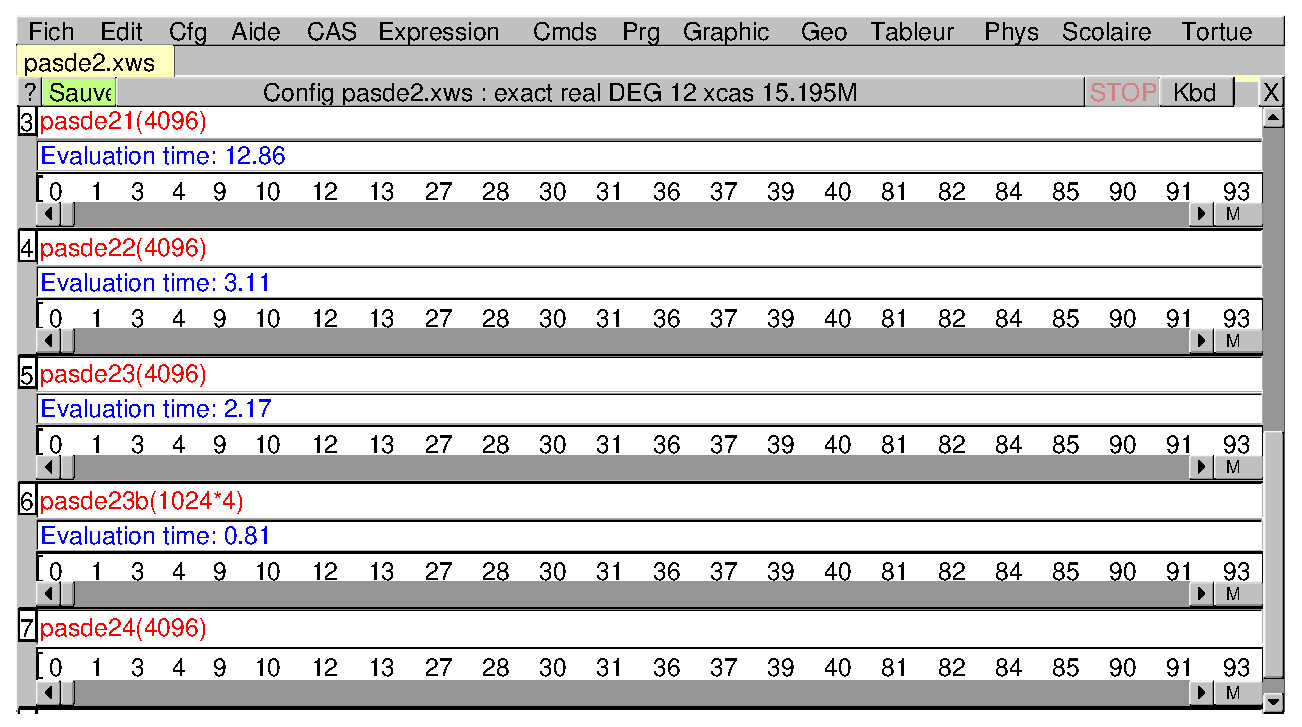
\includegraphics[width=\textwidth]{pasde2}

Ce qui montre que le dernier algorithme est le meilleur...
\end{enumerate}
\section{\'Ecriture d'un entier dans une base rationnelle}
Soient deux entiers $p,q$, premiers entre eux tel que $q<p$. 
On veut \'ecrire un entier $n$ sous la forme :
$$n=\sum_{k=0}^{s-1} n_k(\frac{p}{q})^k \mbox{ avec } n_k<p $$
On d\'efinit la suite :\\
$u(0)=n, u(1)=iquo(u(0),p)*q, u(k+1)=iquo(u(k),p)*q$ 
$u$ est une suite d\'ecroissante donc il existe $s$ tel que $u(s)=0$.\\
On a :\\
$u(0)=iquo(u(0,p)*p+irem(u(0),p)=u(1)*p/q+irem(u(0),p)$\\
$u(1)=iquo(u(1,p)*p+irem(u(1),p)=u(2)*p/q+irem(u(1),p)$\\
On pose $n_0=irem(u(0),p)$\\
Donc :\\
$q^{s-1}u(0)=u(1)*p*q^{s-2}+q^{s-1}n_0$\\
et par it\'eration :\\
$pq^{s-2}u(1)=u(2)p^2q^{s-3}+pq^{s-2}n_1$ avec $n_1==irem(u(1),p)$\\
...\\
$q^{s-1}u(0)=\sum_{k=0}^{s-1}p^kq^{s-k-1}n_k$\\
ou encore :\\
$n=u(0)=\sum_{k=0}^{s-1}p^kq^{-k}n_k$\\
Cette \'ecriture est unique : on raisonne par r\'ecurrencesur $n$.\\
Le d\'eveloppement est unique pour tous les $n<p$.\\
Si il y a unicit\'e pour tous les entiers $m<n$ alors si on a 2 d\'eveloppements
de n :\\
$n==\sum_{k=0}^{s-1}p^kq^{-k}a_k$ et $n==\sum_{k=0}^{s-1}p^kq^{-k}b_k$
puisque $n=a_0+p*\sum_{k=1}^{s-1}p^{k-1}q^{-k}a_k=b_0+p*\sum_{k=1}^{s-1}p^{k-1}q^{-k}b_k=$ on en d\'eduit que $a_0=b_0=\mbox{\tt irem}(n,p)$ et on applique 
l'hypoth\`ese de r\'ecurrence \`a {\tt iquo}$(n,p)*q$ qui est strictement inf\'erieur \`a $n$.\\
On \'ecrit le programme {\tt dev} qui renvoie la liste de dimension $s$ :\\
$[n_0,n_1..n_{s-1}]$ et le programme {\tt verif} qui effectue la v\'erification.
\begin{verbatim}
dev(n,p,q):={
local L,s,u;
si gcd(p,q)!=1 ou q>p-1 alors return "erreur"; fsi;
L:=NULL;
si n<p alors return n; fsi;
s:=n;
tantque s>0 faire
u:=irem(s,p);
s:=iquo(s,p)*q;
L:=L,u;
}
return [L];
}
:;
verif(L,p,q):={
local n,s,k;
n:=L[0];
s:=size(L);
pour k de 1 jusque s-1 faire
n:=n+L[k]*(p/q)^k;
fpour;
return n;
}:;
\end{verbatim}
On tape :\\
{\tt L:=dev(33,3,2)}
On obtient :\\
{\tt [0,1,2,2,1,2]}\\
On tape :\\
{\tt verif(L,3,2)}
On obtient :\\
{\tt 33}\\
On tape :\\
{\tt L:=dev(133,13,8)}
On obtient :\\
{\tt [3,2,9,11,8]}\\
On tape :\\
{\tt verif(L,13,8)}
On obtient :\\
{\tt 133}
\section{Traduction Xcas de l'algorithme de H\"orner}\index{symb2poly}\index{poly2symb}\index{horner}\label{sec:horner}
Soit un polyn\^ome $P$ donn\'e sous la forme d'une liste {\tt l} form\'ee par 
les coefficients de $P$ selon les puissances d\'ecroissantes.\\
{\tt hornerl(l,a)} renvoie une liste form\'ee par la valeur {\tt val} 
du polyn\^ome en $x=a$ et par la liste {\tt lq} des coefficients selon les 
puissances d\'ecroissantes du quotient $Q(x)$ de $P(x)$ par $(x-a)$.\\
On a :\\
${\tt P(a)=l[0]*a^p+l[1]*a^{p-1}+...+l[p]=}$\\
${\tt l[p]+a*(l[p-1]+a*(l[p-2]+...+a*(l[1]+a*l[0])))}$\\
${\tt P(x)=l[0]*x^p+l[1]*x^{p-1}+...+l[p]=}$\\
${\tt (x-a)*(lq[0]*x^{p-1}+...lq[p-1])+val}$ \\
donc ${\tt val=P(a)}$
et {\tt p=s-1} si {\tt s} est la longueur de la liste {\tt l} donc :\\
{\tt lq[0]=l[0]\\
lq[1]=a*lq[0]+l[1]\\
lq[j]=a*lq[j-1]+l[j]\\
....\\
val=a*lq[p-1]+l[p]}
\begin{verbatim}
hornerl(l,a):={
local s,val,lq,j;
s:=size(l);
//on traite les polys constants (de degre=0) 
if (s==1) {return [l[0],[0]]};
// si s>1
lq:=[];
val:=0;
for (j:=0;j<s-1;j++) {
val:=val*a+l[j];
lq:=append(lq,val);
}
val:=val*a+l[s-1];
return([val,lq]);
};
\end{verbatim}
On tape :\\
{\tt hornerl([1,2,4],12)}\\
On obtient :\\
{\tt  [172,[1,14]]}\\
ce qui veut dire que :\\
$x^2+2x+4=(x+14)(x-12)+172$\\
Si le polyn\^ome est donn\'e avec son \'ecriture habituelle.\\
Pour utiliser la fonction pr\'ec\'edente on a alors besoin des deux 
fonctions :\\
 {\tt symb2poly} qui transforme un  polyn\^ome en la liste de ses
coefficients selon les puissances d\'ecroissantes.\\
{\tt poly2symb} qui transforme une liste en l'\'ecriture habituelle du 
polyn\^ome ayant cette pour coefficients selon les puissances d\'ecroissantes. 
\begin{verbatim}
hornerp(p,a,x):={
//ne marche pas pour les polys constants (de degre=0) 
local l,val,lh;
l:=symb2poly(p,x);
lh:=hornerl(l,a);
p:=poly2symb(lh[1],x);
val:=lh[0];
return([val,p]);
};
\end{verbatim}
On tape :\\
{\tt hornerp(x\verb|^|2+2x+4,12,x)}\\
On obtient :\\
{\tt  172,x+14}\\
On tape :\\
{\tt hornerp(y\verb|^|2+2y+4,12,y)}\\
On obtient :\\
{\tt  172,y+14}\\
Dans {\tt Xcas}, il existe la fonction {\tt horner} qui calcule selon la 
m\'ethode de H\"orner la valeur d'un polyn\^ome (donn\'e sous forme de liste 
ou par son expression) en un point :\\
On tape :\\
{\tt horner(x\verb|^|2+2x+4,12)}\\
On obtient :\\
{\tt  172}\\
On tape :\\
{\tt horner(y\verb|^|2+2y+4,12,y)}\\
On obtient :\\
{\tt  172}\\
On tape :\\
{\tt horner([1,2,4],12)}\\
On obtient :\\
{\tt  172}
\subsection{Un autre exercice et sa solution}
Trouver le plus petit entier positif $n$, tel que $n$, $2n$, $3n$, $4n$, $5n$,
 $6n$ contiennent exactement les mêmes chiffres.\\
On tape la fonction bool\'eenne qui teste si les entiers $n$ et $m$ ont des 
chiffres identiques.
On se sert de la fonction {\tt string} qui transforme un entier en une chaine de caract\`eres, puis on 
transforme cette chaine en la liste de ses caract\`eres ou en son code de Ascii, puis on 
trie cette liste.\\
On tape :
\begin{verbatim}
chiffreid(n,m):={
local S1,S2,s1,s2,L1,L2,k;
  S1:=string(n);s1:=size(S1);
  S2:=string(m);s2:=size(S2);
  si s1!=s2 alors retourne faux; fsi;
  L1:=[sort(S1[k]$(k=0..s1-1))]; 
  L2:=[sort(S2[k]$(k=0..s1-1))];
  retourne L1==L2;
}:;
\end{verbatim}
ou
\begin{verbatim}
chiffreid(n,m):={
local S1,S2,s1,s2,L1,L2,k;
  S1:=string(n);s1:=size(S1);
  S2:=string(m);s2:=size(S2);
  si s1!=s2 alors retourne faux; fsi;
  L1:=sort(asc(S1)); 
  L2:=sort(asc(S2));
  retourne L1==L2;
}:;
\end{verbatim}On tape la fonction bool\'eenne qui teste si les entiers $n$, $2n$, $3n$, $4n$, 
$5n$, $6n$ ont des chiffres identiques. Si cela est le cas on 
sait que $n$ est divisible par 3 puisque la somme des chiffres de $n$ est \'egale la somme des chiffres 
de $3n$.\\
On tape :
\begin{verbatim}
chiffreid16(n):={
  local k;
  si irem(n,3)!=0 alors retourne faux; fsi;
  pour k de 6 jusque 2 pas -1 faire 
  si chiffreid(n,k*n)==faux alors retourne faux fsi;
  fpour;
  retourne vrai;
  }:;
\end{verbatim}
On tape la fonction qui renvoie le plus petit entier positif $n$, tel que $n$, 
$2n$, $3n$, $4n$, $5n$, $6n$ contiennent exactement les mêmes chiffres.\\
On tape : 
\begin{verbatim}
ppchiffreid():={
local n;
n:=3;
tantque chiffreid16(n)==faux faire 
  n:=n+3;
 ftantque;
retourne n; 
  }:;
\end{verbatim}
On tape :\\
{\tt ppchiffreid()}\\
On obtient :\\
{\tt 142857}\\
On v\'erifie :\\
On tape :\\
{\tt n:=142857;2*n;3*n;4*n;5*n;6*n}\\
On obtient ;\\
{\tt 142857,285714,428571,571428,714285,857142} 
On peut changer le programme ci-dessus pour savoir qui est le $n$ suivant en 
initialisant $n$ \`a 142860. On trouve alors 1428570.\\
Puis on change \`a nouveau le programme ci-dessus pour savoir qui est le $n$ suivant en 
initialisant $n$ \`a 1428573. On trouve alors 1429857.\\
Puis par curiosit\'e, on cherche le suivant (mais c'est long !), on trouve 14285700.\\
On a donc le d\'ebut de cette suite :
{\tt 142857, 1428570, 1429857, 14285700, 14298570}

\section{Savoir si le polyn\^ome $A$ est divisible par $B$}
\subsection{Programmation de la fonction bool\'eenne {\tt estdivpoly}}
On va \'ecrire la fonction r\'ecursive {\tt estdivpoly} qui a comme arguments, 
deux polyn\^omes  {\tt A} et {\tt B} \'ecrits sous forme symbolique et qui 
renverra {\tt 1} si {\tt A} est divisible par {\tt B} et {\tt 0} sinon.\\
On rappelle que {\tt degree(A)} renvoie le degr\'e de {\tt A} et que
{\tt valuation(A)}  renvoie la valuation de {\tt A}
(la plus petite puissance de {\tt A}). 
 
Pour Savoir si {\tt A} est divisible par {\tt B}, on s'interesse aux termes de 
plus haut degr\'e et de plus bas degr\'e de {\tt A} et {\tt B} : c'est \`a dire
qu'a chaque \'etape on essaye de faire la division par les 2 bouts ....\\
Par exemple si :\\
{\tt A=x\verb|^|3+2*x-3} et {\tt B=x\verb|^|2+x} on sait que {\tt A} n'est pas 
divisible par {\tt B} car {\tt -3} n'est pas divisible par {\tt x},\\
ou encore si :\\
{\tt A=x\verb|^|3+2*x\verb|^|2} et {\tt B=x\verb|^|2+1} on sait que {\tt A} 
n'est pas divisible par {\tt B} car le quotient aurait pour degr\'e
{\tt 3-2=1} et pour valuation {\tt 2-0=2}, ce qui est impossible {\tt 1<2} (le 
degr\'e n'peut pas \^etre inf\'erieur \`a la valuation. \\ 
\begin{verbatim}
estdivpoly(A,B):={
  local da,db,va,vb,dq,vq,dva,dvb,dvq,Q,Ca,Cb;
  da:=degree(A);
  va:=valuation(A);
  dva:=da-va;
  db:=degree(B);
  vb:=valuation(B);
  dvb:=db-vb;
  if (A==0) then return 1;end_if;
  if ((da<db) or (va<vb)) then return 0;end_if;
  if ((dva==0) and (dvb>0)) then return 0;end_if;
  if ((dva>=0) and (dvb==0)) then return 1;end_if;
  Cb:=coeffs(B);
  if ((dva>0) and (dvb>0)) then 
  dq:=da-db;
  vq:=va-vb;
  dvq:=dq-vq;
  if (dvq<0) then return 0;end_if;
  Ca:=coeffs(A); 
  Q:=Ca[0]/Cb[0]*x^(dq);
  if (dvq==0) then 
  A:=normal(A-B*Q);
  else
  Q:=Q+Ca[dva]/Cb[dvb]*x^(vq);  
  A:=normal(A-B*Q);
  end_if;
  da:=degree(A);
  va:=valuation(A);
   end_if;
  return estdivpoly(A,B);
};
\end{verbatim}
On tape :
{\tt A:=normal((x\verb|^|4-x\verb|^|3+x\verb|^|2-1)*(x\verb|^|5-x\verb|^|3+x\verb|^|2-1)}\\
puis,\\
{\tt estdivpoly(A,x\verb|^|4-x\verb|^|3+x\verb|^|2-1)}\\
On obtient :\\
{\tt 1}
\subsection{Autre version du programme pr\'ecedent : {\tt quoexpoly}}
Lorsque {\tt A} est divisible par {\tt B} on peut en modifiant le programme
pr\'ec\'edent avoir facilement le quotient exact de {\tt A} par {\tt B}.\\
On \'ecrit la fonction r\'ecursive {\tt quoexpoly} qui a trois arguments, 
deux polyn\^omes  {\tt A} et {\tt B} \'ecrits sous forme symbolique et {\tt 0}.
{\tt quoexpoly} renverra {\tt 1,Q} si {\tt A=B*Q} et {\tt 0} sinon.\\
Puis on \'ecrit la fonction {\tt quopoly(A,B)} qui est \'egale \`a 
{\tt quoexpoly(A,B,0)}.
\begin{verbatim}
quoexpoly(A,B,SQ):={
  local da,db,va,vb,dq,vq,dva,dvb,dvq,Q,Ca,Cb;
  da:=degree(A);
  va:=valuation(A);
  dva:=da-va;
  db:=degree(B);
  vb:=valuation(B);
  dvb:=db-vb;
  if (A==0) then return 1,SQ;end_if;
  if ((da<db) or (va<vb)) then return 0;end_if;
  if ((dva==0) and (dvb>0)) then return 0;end_if;
  if ((dva>=0) and (dvb==0)) then return 1,normal(SQ+normal(A/B));end_if;
  Cb:=coeffs(B);
  if ((dva>0) and (dvb>0)) then 
  dq:=da-db;
  vq:=va-vb;
  dvq:=dq-vq;
  if (dvq<0) then return 0;end_if;
  Ca:=coeffs(A); 
  Q:=Ca[0]/Cb[0]*x^(dq);
  if (dvq==0) then 
  A:=normal(A-B*Q);
  SQ:=normal(SQ+Q);
  else
  Q:=Q+Ca[dva]/Cb[dvb]*x^(vq);  
  A:=normal(A-B*Q);
   SQ:=normal(SQ+Q);
  end_if;
  da:=degree(A);
  va:=valuation(A);
   end_if;
  return quoexpoly(A,B,SQ);
};
estquopoly(A,B):=quoexpoly(A,B,0);
\end{verbatim}
On tape :
{\tt A:=normal((x\verb|^|4-x\verb|^|3+x\verb|^|2-1)*(x\verb|^|5-x\verb|^|3+x\verb|^|2-1)}\\
puis,\\
{\tt estquopoly(A,x\verb|^|4-x\verb|^|3+x\verb|^|2-1)}\\
On obtient :\\
{\tt 1,x\verb|^|5-x\verb|^|3+x\verb|^|2-1}

\section{Affichage d'un nombre en une cha\^{\i}ne comprenant des espaces}
\subsection{Affichage d'un nombre entier par tranches de $p$ chiffres}
Pour rendre plus facile la lecture d'un grand nombre entier, on veut l'afficher
par tranches, c'est \`a dire selon une cha\^{\i}ne de caract\`eres constitu\'ees
par les $p$ premiers chiffres du nombre et d'un espace, puis les $p$ suivants 
etc...
On \'ecrit le programme qui va afficher le nombre $n$ par tranches de $p$ 
chiffres: 
\begin{verbatim}
affichen(n,p):={
local reste,result,s;
result:="";
while (n>10^p) {
//on transforme irem(n,10^p) en une chaine
reste:=cat(irem(n,10^p),"");
s:=size(reste);
//on ajoute l'espace et les zeros qui manquent
reste:=cat(" ",op(newList(p-s)),reste);
n:=iquo(n,10^p);
//on concatene reste avec result 
result:=cat(reste,result);
}
reste:=cat(n);
return cat(reste,result);
};
\end{verbatim}
On tape :\\
{\tt affichen(1234567,3)}
On obtient :\\
{\tt "1 234 567"}
\subsection{Transformation d'un affichage par tranches en un nombre entier}
Pour avoir la transformation inverse, on va transformer une cha\^{\i}ne
comportant des chiffres et un autre caract\`ere (par exemple un espace) en un 
nombre entier.\\
On \'ecrit le programme :
\begin{verbatim}
enleve(chn,ch):={
local l,s;
s:=length(chn)-1;
//on transforme chn en une liste de ces lettres
//puis, on enleve le caractere ch de cette liste
l:=remove(x->(ord(x)==ord(ch)),seq(chn[k],k,0,s));
//on transforme la liste en chaine
return expr(char(ord(l)));
};
\end{verbatim}
On peut aussi remplacer la derni\`ere ligne :\\
{\tt return char(ord(l))}\\
({\tt ord(l)} transforme la liste de caract\`eres en la liste de leurs codes 
ascii et {\tt char} transforme la liste des codes ascii en une cha\^{\i}ne).\\
par :\\
{\tt return cat(op(l))}\\
car {\tt op(l)} transforme la liste en une s\'equence et {\tt cat}
concat\`ene les \'el\'ements de cette s\'equence en une cha\^{\i}ne.
On tape :\\
{\tt enleve("1 234 567"," ")}
On obtient :\\
{\tt 1234567}
\subsection{Affichage d'un nombre d\'ecimal de [0,1[ par tranches de $p$ chiffres}
Pour rendre plus facile la lecture d'un nombre d\'ecimal de [0,1[, on veut 
l'afficher par tranches, c'est \`a dire selon une cha\^{\i}ne de caract\`eres 
constitu\'ees par les $p$ premi\`eres d\'ecimales du nombre et d'un espace, 
puis les $p$ suivants etc...
On suppose que l'\'ecriture de $d$ comporte un point ($.$) suivi des 
d\'ecimales et ne comporte pas d'exposant (pas de $e4$)
 
On \'ecrit le programme qui va afficher le nombre $d$ par tranches de $p$ 
chiffres: 
\begin{verbatim}
affiched(d,p):={
local deb,result;
//on suppose 0<=d<1
d:=cat(d,"");
if (d[0]=="0") {d:=tail(d);}
if (expr(tail(d))<10^p){return d;}
deb:=mid(d,0,p+1);
result:=cat(deb," ");
d:=mid(d,p+1);
while (expr(d)>10^p) {
deb:=mid(d,0,p);
result:=cat(result,deb," ");
d:=mid(d,p);
}
return cat(result,d);
};
\end{verbatim}
On tape :\\
{\tt affiched(0.1234567,3)}\\
On obtient :\\
{\tt ".123 456 7"}\\
{\bf Remarque}\\
La commande {\tt enleve(affiched(d,3)," ")} permet encore de retrouver {\tt d}.
\begin{verbatim}
enleve(chn,ch):={
local l,s;
s:=length(chn)-1;
//on transforme chn en une liste de ces lettres
//puis, on enleve le caractere ch de cette liste
l:=remove(x->(ord(x)==ord(ch)),seq(chn[k],k,0,s));
//on transforme la liste en chaine
return expr(char(ord(l)));
};
\end{verbatim}
\subsection{Affichage d'un nombre d\'ecimal par tranches de $p$ chiffres}
Pour rendre plus facile la lecture d'un nombre d\'ecimal, on veut 
l'afficher par tranches, c'est \`a dire selon une cha\^{\i}ne de caract\`eres 
constitu\'ees par sa partie enti\`ere \'ecrite par tranches de $p$ chiffres,
puis ses $p$ premi\`eres d\'ecimales du nombre et d'un espace, puis les $p$ 
suivants etc...\\
Ici, le nombre $f$ peut comporter un exposant \`a la fin de son \'ecriture.\\
On \'ecrit le programme qui va afficher le nombre d\'ecimal $f$ par tranches 
de $p$ chiffres : 
\begin{verbatim}
//pour les flottants f utiliser affichef
// appelle affichen et affiched 
//par exemple affichef(1234.12345,3)
affichef(f,p):={
local deb,result,s,indicep,fn,fd,indicee;
//on suppose f>1
f:=cat(f);
s:=size(f)-1;
indicep:=member(".",seq(f[k],k,0,s));
indicee:=member("e",seq(f[k],k,0,s));
if (indicep!=0) {
fn:=mid(f,0,indicep-1);
fd:=mid(f,indicep-1);
if (indicee!=0) {
return affichen(expr(fn),p)+affiched(expr(mid(fd,0,
indicee-1)),p)+mid(fd,indicee-1);}
return affichen(expr(fn),p)+affiched(expr(fd),p)
}
return affichen(expr(f),p);
};
\end{verbatim}
On tape :\\ 
{\tt affichef(1234567.1234567,3)} \\
On obtient (pour 12 chiffres significatifs) :\\
{\tt "1 234 567.123 46"}\\
On obtient (pour 14 chiffres significatifs) :\\
{\tt "1 234 567.123 456 7"}\\
On obtient (pour 15 chiffres significatifs) :\\
{\tt "0.123 456 712 345 670 0*e7"}\\
{\bf Remarque}\\
La commande {\tt enleve(affichef(q,3)," ")} permet encore de retrouver {\tt q}.
\begin{verbatim}
enleve(chn,ch):={
local l,s;
s:=length(chn)-1;
//on transforme chn en une liste de ces lettres
//puis, on enleve le caractere ch de cette liste
l:=remove(x->(ord(x)==ord(ch)),seq(chn[k],k,0,s));
//on transforme la liste en chaine
return expr(char(ord(l)));
};
\end{verbatim}
\section{\'Ecriture d\'ecimale d'un nombre rationnel}
\subsection{Algorithme de la potence}
Pour obtenir la partie enti\`ere et le d\'eveloppement d\'ecimal de 
$\displaystyle \frac{a}{b}$, on va construire deux listes :
{\tt L1} la liste des restes et {\tt L2} 
la liste des quotients obtenus par l'algorithme de la potence .\\
On met le quotient $q$ dans {\tt L1} et le reste $r$ dans {\tt L2}.\\
On a ainsi, la partie enti\`ere de $\displaystyle \frac{a}{b}$ dans {\tt L1}
et comme $\displaystyle \frac{a}{b}=q+\frac{r}{b}$ on cherche la partie enti\`ere de $\displaystyle \frac{10*r}{b}$ qui va rallonger {\tt L1} etc...

Si on veut, par exemple, le d\'eveloppement d\'ecimale de 
$\displaystyle \frac{278}{31}$ on cherche :\\
le quotient $q=8$  et le reste $r=30$ de la divison euclidienne de 278 par 31.\\ La partie enti\`ere est donc 8 et, on met 8{\tt L1} .
Pour avoir la partie d\'ecimale de $\displaystyle \frac{278}{31}$, on fait 
comme \`a la main l'algorithme de
la potence : on  multiplie le reste trouv\'e par 10, on trouve 300  
puis on le divise par 31 : le quotient trouv\'e 9 est 
rajout\'e \`a {\tt L1} et le reste est rajout\'e \`a {\tt L2} etc...\\
On \'ecrit la fonction potence qui renvoie dans la premi\`ere liste 
la partie enti\`ere puis les $n$ d\'ecimales de $\frac{a}{b}$ et dans la 
deuxi\`eme liste les restes successifs obtenus.
\begin{verbatim}
potence(a,b,n):={
 local L1,L2,k;
 b0:=b;
 b:=iquo(a,b0);
 a:=irem(a,b0);
 L1:=[b];
 L2:=[a];
 for (k:=1;k<=n and a!=0;k++){
    b:=iquo(a*10,b0);
    a:=irem(a*10,b0);
    L2:=append(L2,a);
    L1:=append(L1,b);
 };
 return([L1,L2]);
};
\end{verbatim}
En ex\'ecutant {\tt potence(278,31,20)}, on lit la partie enti\`ere de 
$\displaystyle \frac{278}{31}$ et les chiffres de sa partie d\'ecimale dans la 
premi\`ere liste et, la suite des restes dans la deuxi\`eme liste.\\
{\bf Exercice}\\
\'Ecrire la partie enti\`ere et le d\'eveloppement d\'ecimal de :\\
 $a=\displaystyle\frac{11}{7}$,  $b=\displaystyle\frac{15}{14}$  et 
$c=\displaystyle\frac{17}{28}$.\\
Calculer $a-b$ et  $a-c$ 
et donner leur partie enti\`ere et leur
 d\'eveloppement d\'ecimal.\\
Que remarqez-vous ?\\  
{\bf Exercice}
Comment modifier  {\tt L1} et {\tt L2} pour que les chiffres de la 
partie d\'ecimale de $\displaystyle\frac{a}{b}$ se lisent par paquet de trois 
chiffres dans {\tt L1}.\\
 Avec l'exemple $\displaystyle\frac{278}{31}$ on veut obtenir :
{\tt L1=[8,967,741,935 ...]}\\
Tester votre modification pour $\displaystyle\frac{349}{1332}$.\\
Que remarquez vous ? 
\subsection{Avec un programme}
{\tt division(a,b,n,t)} donne la partie enti\`ere suivie de $n$ paquets de
 $t$ d\'ecimales (i.e. des $n*t$ premi\`eres 
d\'ecimales) de $\displaystyle\frac{a}{b}$.
\begin{verbatim} 
division(a,b,n,t):={
local L1,L2,p,q,r,k;
L1:=[iquo(a,b)];
r:=irem(a,b);
for (k:=1;k<=n and r!=0;k++) {
q:=iquo(r*10^t,b);
//10^(p-1)<= q <10^p
if (q==0) {p:=1} else {p:=floor(ln(q)/ln(10)+1)};
//on complete par des zeros pour avoir un paquet de t decimales
for (j:=p+1;j<=t;j++){
L1:=append(L1,0);
}
L1:=append(L1,q);
r:=irem(r*10^t,b);
}
return(L1,r);
};
\end{verbatim}
On tape pour avoir 5*6=30 decimales :\\
{\tt division(2669,201,6,5)}\\
On obtient :\\
{\tt [13,27860,69651,74129,35323,38308,45771],29} 
\subsection{Construction d'un rationnel}
\noindent Trouver un nombre rationnel  qui s'\'ecrit :\\
$0.123123123123...$ se terminant par une suite illimit\'ee de  $123$.\\ 
Trouver un nombre rationnel qui s'\'ecrit :\\
$0.120123123123...$ se terminant par une suite illimit\'ee de  $123$.\\
\'Ecrire un  programme qui permet de trouver un nombre rationnel \`a partir 
d'un d\'eveloppement d\'ecimal p\'eriodique.\\
R\'eponse :\\
On \'ecrit la fonction {\tt rationnel} qui a comme le param\`etre deux listes 
{\tt l1} et {\tt l2} :\\
- {\tt l1} d\'esigne la partie non p\'eriodique de ce d\'eveloppement et 
{\tt l1[0]} d\'esigne la partie enti\`ere.\\
- {\tt l2}  repr\'esente un d\'eveloppement d\'ecimal p\'eriodique.

\begin{verbatim} 
rationnel(l1,l2):={
//l1 et l2 sont non vides
local pui,s1,s2,n,p,np,pui,k;
pui:=10;
s2:=size(l2);
n:=l2[0];
for (k:=1;k<s2;k++){
pui:=pui*10;
n:=n*10+l2[k];
}
// 0.123123...=123/999 
p:=n/(pui-1);
//np partie non periodique
np:=l1[0];
s1:=size(l1);
pui:=1;
for (k:=1;k<s1;k++){
pui:=pui*10;
np:=np+l1[k]/pui;
}
//pui=10^(s1-1) 
return(np+p/pui);
};
\end{verbatim}
\section{D\'eveloppement en fraction continue}
\subsection{D\'eveloppement en fraction continue d'un rationnel}
\subsubsection{Les d\'efinitions}
{\bf  Th\'eor\`eme1} Si $a$ et $b$ sont des entiers naturels premiers entre
 eux, alors il existe des entiers naturels 
$a_0,a_1,...,a_n$ ($0 \leq n$) tels que :
$$\frac{a}{b}=a_0+\frac{1}{a_1+\frac{1}{a_2+\frac{1}{...a_{n-2}+\frac{1}{a_{n-1}+\frac{1}{a_n}}}}}$$
Si  $b\leq a$ les $aj$ sont non nuls et, si $a<b$ alors $a_0=0$ et les autres 
$a_j$ sont non nuls.\\ 
{\bf D\'efinition}
On pose alors $\displaystyle\frac{a}{b}=(a_0,a1,...a_n)$ et on dit que 
$(a_0,a1,...a_n)$ 
est une fraction continue : c'est le d\'eveloppement en fraction continue de
$\displaystyle \frac{a}{b}$.\\
{\bf Remarque} si $b\leq a$ et si $\displaystyle\frac{a}{b}=(a_0,a1,...a_n)$ 
alors $\displaystyle\frac{b}{a}=(0,a_0,a1,...a_n)$.\\
{\bf R\'eduite et reste}
On dit que la fraction $\displaystyle\frac{P_p}{Q_p}$ \'egale \`a la
fraction continue $(a_0,a1,...a_{p})$, o\`u $p\leq n$, est la r\'eduite de 
rang $p$ de $\displaystyle\frac{a}{b}$ ou que c'est le d\'eveloppement en  
fraction continue d'ordre $p$ de $\displaystyle\frac{a}{b}$.\\
 On dit que 
$r=(0,a_{p+1},..,a_n)$ est le reste du d\'eveloppement d'ordre $p$ ($r<1$)
et on a $\displaystyle\frac{a}{b}=(a_0,a1,...a_{p}+r)=(a_0,a1,...a_{p},1/r)$,\\
$\displaystyle\frac{a}{b}=a_0+\frac{1}{a_1+\frac{1}{a_2+\frac{1}{...a_{p-3}+\frac{1}{a_{p-2}+\frac{1}{a_{p}+r}}}}}$.\\ 
\subsubsection{Propri\'et\'es des r\'eduites}
Si $\displaystyle\frac{P_p}{Q_p}$ \'egale \`a la
fraction continue $(a_0,a1,...a_{p})$, o\`u $p\leq n$, est la r\'eduite de 
rang $p$ de $\displaystyle\frac{a}{b}=(a_0,a1,...a_{n})$, on a :\\
$P_0=a_0$\\
$Q_0=1$\\
$P_1=a_0*a_1+1$\\
$Q_1=a_1$\\
$P_p=P_{p-1}*a_p+P_{p-2}$\\ 
$Q_p=Q_{p-1}*a_p+Q_{p-2}$\\
En effet on le montre par r\'ecurrence :\\
$P_2/Q_2=a_0+a_2/(a_1a_2+1)$ donc\\
$P_2=a_2(a_0+a_1+1)+a_0=a_2P_1+P_0$ et \\
$Q_2=a_2a_1+1=a_2Q_1+Q_0$\\
$(a_0,a_1,...,a_p+1/a_{p+1})=\frac{P_{p+1}}{Q_{p+1}}$ donc\\
$P_{p+1}/Q_{p+1}=((a_{p}+1/a_{p+1})P_{p-1}+P_{p-2})/((a_{p}+1/a_{p+1})Q_{p-1}+Q_{p-2})$\\
$P_{p+1}=a_{p+1}(a_pP_{p-1}+P_{p-2})+P_{p-1}=a_{p+1}P_p+P_{p-1}$ et \\
$Q_{p+1}=a_{p+1}(a_pQ_{p-1}+Q_{p-2})+Q_{p-1}=a_{p+1}Q_{p}+Q_{p-1}$
\subsubsection{Les programmes}
{\bf Le programme f2dfc :} \\
On veut transformer une fraction en son d\'eveloppement en fraction continue :\\${\tt f2dfc(a/b)=(a_0, a_1,...a_n)}$.\\
Pour obtenir le d\'eveloppement en fraction continue de $a/b$, on cherche le 
quotient $q$ et le reste $r$ de la division euclidienne de $a$ par $b$.
On a :  $q=a_0$ et $a/b=a_0+r/b=a_0+1/(b/r)$ et, on continue en cherchant
 la partie enti\'ere de $b/r$ qui sera $a_1$....On reconnait
 l'algorithme d'Euclide : la suite $(a_0, a_1,...a_n)$ est donc la suite 
des quotients de l 'algorithme d'Euclide.\\
On \'ecrit le programme : 
\begin{verbatim}
f2dfc(fract):={
local r,q,l,lres,a,b;
l:=f2nd(fract);
a:=l[0];
b:=l[1];
lres:=[];
while (b>0) {
q:=iquo(a,b)
lres:=concat(lres,q);
r:=irem(a,b); 
a:=b;
b:=r:
}
return lres;
}
\end{verbatim}
On tape :\\
{\tt f2dfc(2599/357)}\\
On obtient :\\
{\tt [7,3,1,1,3,14]}\\
{\bf Le programme f2reduites d'un rationnel et l'identit\'e de B\'ezout :} 
On veut obtenir la suite des r\'eduites de $a/b$.\\
L'algorithme pour obtenir les r\'eduites ressemble beaucoup \`a l'algorithme 
utilis\'e pour obtenir les coefficients $u$ et $v$ de l'identit\'e de 
B\'ezout (cf \ref{sec:bezout}).\\
En effet on a :\\
$P_0=a_0=a_0*1+0$ alors que  $v_0=0$ \\
$Q_0=1=a_0*0+1$ alors que  $u_0=1$\\
$P_1=a_0a_1+1=P_0*a_1+1$ alors que  $v_1=1$\\
$Q_1=a_1=a_1*Q_0+0$ alors que $u_1=0$\\
$P_p=P_{p-1}*a_p+P_{p-2}$ alors que $v_p=v_{p-2}-a_{p-2}v_{p-1}$\\ 
$Q_p=Q_{p-1}*a_p+Q_{p-2}$ alors que $u_p=u_{p-2}-a_{p-2}u_{p-1}$\\
Ainsi :\\
$P_0=0+a_0*1=v_0-a_0*v_1=-v_2$ \\
$P_1=1+P_0*a_1=v_1-v_2*a_1=v_3$\\
$P_2=P_0+P_1*a_2=-v_2+v_3*a_2=-(v_2-v_3*a_2)=-v_4$\\
On a donc pour tout $p \geq 0$, si $a_p$ est la suite des quotients de 
l'algorithme d'Euclide :\\ 
$Q_p=Q_{p-1}*a_p+Q_{p-2}$ avec $Q_{-2}=1=u_0$ et $Q_{-1}=0=u_1$ et,\\
$P_p=P_{p-1}*a_p+P_{p-2}$ avec $P_{-2}=0=v_0$ et $P_{-1}=1=v_1$\\ 
Dans l'algorithme de B\'ezout on a :\\
$u_p=-u_{p-1}*a_{p-2}+u_{p-2}$ et $v_p=-v_{p-1}*a_{p-2}+v_{p-2}$ 
$Q_0=0+u_2$ donc $Q_1=-u_3$, $Q_2=u_4$ etc...donc $Q_n=(-1)^nu_{n+2}$ et,\\
$P_0=-v_2+0$ donc $P_1=v_3$, $P_2=-v_4$ etc...donc $P_n=(-1)^{n+1}v_{n+2}$.\\
Donc $P_n/Q_n=-v_{n+2}/u_{n+2}$\\
Donc la suite $Q_j/P_j$ est donc la suite des $-u/v$.\\
On \'ecrit le programme (calqu\'e sur le programme {\tt Bezout} avec les 
listes) qui transforme une fraction en son d\'eveloppement en fraction continue
suivi de la suite de ces r\'eduites : 
\begin{verbatim}
f2reduites(fract):={
local lr,q,l,lres,la,lb,lq;
l:=f2nd(fract);
//a:=l[0];b:=l[1];
la:=[1,0,l[0]];
lb:=[0,1,l[1]];
lq:=[];
lres:=[];
while (lb[2]>0) {
q:=iquo(la[2],lb[2])
lr:=la-q*lb;
lq:=concat(lq,q);
lres:=concat(lres,-lr[1]/lr[0]);
la:=lb;
lb:=lr;
}
return lq,lres;
}
\end{verbatim}
On tape :\\
{\tt f2reduites(2599/357)}\\
On obtient :\\
{\tt [7,3,1,1,3,14],[7,22/3,29/4,51/7,182/25,2599/357]}\\
{\bf Remarque} :\\
On ne peut pas remplacer :\\
{\tt lr:=la-q*lb;}\\
{\tt lres:=concat(lres,-lr[1]/lr[0])}\\
par :\\
{\tt lr:=la+q*lb;}\\
{\tt lres:=concat(lres,lr[1]/lr[0]);}\\
car alors {\tt lr} n'est plus la suite des restes !\\
{\bf Le programme dfc2reduites d'un rationnel et l'identit\'e de B\'ezout:} 
On veut obtenir la suite des r\'eduites d'une liste $l$ (qui sera par exemple 
le d\'eveloppement en fraction continue d'un rationnel $a/b$) 
On \'ecrit le programme (calqu\'e sur le programme {\tt Bezout} sans les 
listes) qui transforme une liste $[a_0,a_1,..a_n]$ en la 
liste $[a_0,a_0+1/a_1,....,(a_0+1/a_1+1/...+1/a_{n-1}+1/a_n)]$ : 
\begin{verbatim}
dfc2reduites(l):={
local s,p0,q0,p1,q1,p,q,lres,j;
s:=size(l);
lres:=[];
p0:=0;
p1:=1;
q0:=1;
q1:=0;
for (j:=0;j<s;j++){
  p:=p0+l[j]*p1;
  q:=q0+l[j]*q1;
  lres:=concat(lres,p/q);
  p0:=p1;
  q0:=q1;
  p1:=p;
  q1:=q;
}
return lres;
}
\end{verbatim}
On remarquera que :\\
 -la suite des $P$ est initialis\'ee par
$p0$ et $p1$, puis, quand $j=0$, on fait le calcul de $P_0$ qui est mis dans 
$p$, puis, quand $j=1$ on fait 
le calcul de $P_1$ qui est mis dans $p$, etc... et que\\
- la suite des $Q$ est initialis\'ee par :
$q0$ et $q1$, puis, quand $j=0$ on fait le calcul de $Q_0$ qui est mis dans 
$q$, quand $j=1$, on fait
le calcul de $Q_1$ est mis dans $q$, etc...\\
On tape :\\
{\tt dfc2reduites([7,3,1,1,3,14])}\\
On obtient :\\
{\tt [7,22/3,29/4,51/7,182/25,2599/357]}
\subsection{D\'eveloppement en fraction continue d'un r\'eel quelconque}
{\bf  Th\'eor\`eme2} Si $\alpha$ est un nombre r\'eel non rationnel,
 alors il existe des entiers naturels non nuls 
$a_0,a_1,...,a_n$ et un r\'eel $\beta<1$ tels que :
$$\alpha=a_0+\frac{1}{a_1+\frac{1}{a_2+\frac{1}{...a_{n-2}+\frac{1}{a_{n-1}+\frac{1}{a_n+\beta}}}}}$$
On dit que $(a_0,a1,...a_n)$ est le d\'eveloppement en fraction continue 
d'ordre $n+1$ de $\alpha$ et que $\beta$ est le reste de ce d\'eveloppement.\\ 
Un rationnel a un d\'eveloppement en fraction continue fini et 
r\'eciproquement, un d\'eveloppement en fraction continue fini repr\'esente 
un rationnel.\\
Un r\'eel non rationnel a un d\'eveloppement en fraction continue infini.\\
Si  $\alpha$ est un nombre quadratique (i.e. $\alpha$ est racine d'une 
\'equation du second degr\'e), $\alpha$ a un d\'eveloppement en fraction 
continue p\'eriodique et r\'eciproquement, un d\'eveloppement en fraction 
continue p\'eriodique repr\'esente un nombre quadratique.

\subsection{Les programmes}
On va \'ecrire deux fonctions {\tt r2dfc} et {\tt dfc2r}.
\subsubsection{La fonction r2dfc}
{\tt r2dfc(alpha,n)} qui transforme un r\'eel {\tt alpha} en son
d\'eveloppement en fraction continue  et qui renvoie deux listes, soit :\\
- ${\tt [a_0,a_1...a_p],[]}$ avec ${\tt p \leq n}$ o\`u les ${\tt a_j}$ sont 
des entiers, la deuxi\`eme liste est 
vide et la premi\`ere liste est le d\'eveloppement en fraction 
continue de {\tt alpha} (les ${\tt a_j}$ sont des entiers et donc {\tt alpha} 
est une fraction)\\
-  ${\tt [a_0,a_1...a_{n-1},b],[]}$, la deuxi\`eme liste est vide et 
la premi\`ere liste est le d\'eveloppement en fraction 
continue d'ordre $n-1$ de {\tt alpha} suivi de ${\tt b>1}$ (le reste est \'egal \`a 
${\tt 1/b}$), o\`u les ${\tt a_j}$ sont des entiers et {\tt b} est un r\'eel 
plus grand que 1, soit,\\
- ${\tt [a_0,a_1...a_p],[a_r,..a_p]}$ avec ${\tt r\leq p < n}$\\
o\`u les ${\tt a_j}$ sont des entiers, la premi\`ere liste est le 
d\'eveloppement en fraction continue d'ordre $p$ de {\tt alpha} et 
la deuxi\`eme liste repr\'esente la p\'eriode de ced\'eveloppement en fraction 
continue (les ${\tt a_j}$ sont des entiers et donc {\tt alpha} est un nombre 
quadratique)\\.\\ 
On remarquera dans le programme ci-dessous que :\\
${\tt a_0=floor(alpha)=q}$ remplace ${\tt q:=iquo(a,b)}$ lorsque 
{\tt alpha=a/b}\\
et que {\tt r=alpha-q} remplace ${\tt irem(a,b)/b}$ lorsque 
{\tt alpha=a/b}\\
et donc que si {\tt r=alpha-q}, ${\tt a_1=floor(1/r)}$ etc...\\
Le probl\`eme ici est de pouvoir comparer {\tt alpha} et {\tt q} 
c'est \`a dire savoir si {\tt r==0} et pour cela on est oblig\'e de
faire les calculs avec beaucoup de d\'ecimales c'est \`a dire d'augmenter 
le nombre de digits (on tape par exemple {\tt DIGITS:=30}). 
Il faut bien s\^ur rep\'erer la p\'eriode, pour cela on forme la liste 
{\tt lr} des restes successifs. La liste {\tt lq} des parties enti\`eres
 successives forme le d\'ebut du d\'eveloppement en fraction continue.
\begin{verbatim}
r2dfc(alpha,n):={
local r,q,lq,lr,p,j;
q:=floor(alpha);
r:=normal(alpha-q);
lq:=[];
lr:=[];
for (j:=1;j<=n;j:=j+1) {
lq:=concat(lq,q);
if (r==0){return (lq,[]);}
p:=member(r,lr);
if (p) {return (lq,mid(lq,p)):}
lr:=concat(lr,r);
alpha:=normal(1/r);
q:=floor(alpha);
r:=normal(alpha-q);
}
return (concat(lq,alpha),[]);
};
\end{verbatim}
On tape :\\
{\tt dfc2r(sqrt(2),1)}\\
On obtient :\\
{\tt ([1,sqrt(2)+1],[])}\\
On tape :\\
{\tt dfc2r(sqrt(2),2)}\\
On obtient :\\
{\tt ([1,2],[2])}\\
On tape :\\
{\tt dfc2r(pi),6}\\
On obtient :\\
{\tt ([3,7,15,1,292,1,(-33102*pi+103993)/(33215*pi-104348)],[])}
{\bf Remarque}
Le premier argument doit \^etre un nombre exact, car sinon les calculs sont 
faits en mode approch\'e et le test r==0 n'est jamais r\'ealis\'e...
\subsubsection{La fonction dfc2r}
On \'ecrit la fonction r\'eciproque de {\tt r2dfc} qui \`a partir d'un 
d\'eveloppement en fraction continue et d'un reste \'eventuel ou d'un 
d\'eveloppement en fraction continue et d'une p\'eriode \'eventuelle 
renvoie un r\'eel.\\
{\tt dfc2r(d,t)} transforme  en un r\'eel, la liste {\tt d} repr\'esente un
 d\'eveloppement en fraction continue et la liste 
{\tt t} repr\'esente la p\'eriode.\\
On remarquera que lorsque la liste 
{\tt t}  n'est pas vide il faut d\'eterminer le nombre {\tt 0<y<1} qui admet 
cette liste p\'eriodique comme d\'eveloppement en fraction continue et 
pour ce faire r\'esoudre l'\'equation :\\
${\tt y=(0,t_0,...t_{st-1}+y)}$
le reste est alors ${\tt y+d_{s-1}}$ ({\tt s:=size(d)}).\\
On \'ecrit le programme :
\begin{verbatim}
dfc2r(d,t):={
local s,st,alpha,l,ap,k;
s:=size(d);
alpha:=d[s-1];
for (k:=s-2;k>=0;k:=k-1) {alpha:=normal(d[k]+1/alpha);}
if (t==[]) {return normal(alpha);}
st:=size(t);
purge(y);
ap:=t[st-1]+y;
for (k:=st-2;k>=0;k:=k-1) {ap:=normal(t[k]+1/ap);}
l:=solve(y=1/ap,y);
if (l[0]>0){y:=normal(l[0]);}else{y:=normal(l[1]);};
alpha:=d[s-1]+y;
for (k:=s-2;k>=0;k:=k-1) {alpha:=normal(d[k]+1/alpha);}
return(normal(a)lpha);
};
\end{verbatim}
ou avec une \'ecriture plus concise :
\begin{verbatim}
dfc2r(d,t):={
local s,st,alpha,l,ap,k;
s:=size(d);
st:=size(t);
if (st==0) 
  {y:=0;} 
   else 
 {purge(y);
  ap:=t[st-1]+y;
  for (k:=st-2;k>=0;k:=k-1) {ap:=normal(t[k]+1/ap);}
  l:=solve(y=1/ap,y);
  if (l[0]>0){y:=normal(l[0]);}else{y:=normal(l[1]);};
  }
alpha:=d[s-1]+y;
for (k:=s-2;k>=0;k:=k-1) {alpha:=normal(d[k]+1/alpha);}
return(normal(alpha));
};
\end{verbatim}
\subsection{Exemples}
1/ D\'eveloppement en fraction continue de :
${\tt \frac{1393}{972}}$,
${\tt 1+\sqrt{13}}$ et 
${\tt 1-\sqrt{13}}$.\\
On a :\\
{\tt r2dfc(1393/972,3)=[1,2,3,130/31],[]}\\
{\tt r2dfc(1393/972,7)=[1,2,3,4,5,6],[]}\\
et on a bien :\\
{\tt r2dfc(130/31,3)=[4,5,6],[]}\\
{\tt r2dfc(31/130,4)=[0,4,5,6],[]}\\
On peut v\'erifier que :\\
{\tt dfc2r([1,2,3,4,5,6],[])=1393/972}\\
{\tt dfc2r([1,2,3+31/130],[])=dfc2r([1,2,3,130/31],[])=1393/972}\\
On a : \\
{\tt r2dfc(1+sqrt(13),3)=[4,1,1,(sqrt(13)+2)/3],[]}\\
{\tt r2dfc(1+sqrt(13),6)=[4,1,1,1,1,6],[1,1,1,1,6]}\\
{\tt r2dfc(1-sqrt(13),7)=[-3,2,1,1,6,1,1],[1,1,6,1,1]}

2/ Trouver les r\'eels qui ont comme d\'eveloppement en fraction continue :\\
{\tt [2,4,4,4,4,4....]} (suite illimit\'ee de {\tt 4}) et\\
{\tt [1,1,1,1,1,1....]} (suite illimit\'ee de {\tt 1}).\\
On a :\\
{\tt dfc2r([2,4],[4])=sqrt(5)}
ou encore
{\tt dfc2r([2],[4])=sqrt(5)}
On a :\\
{\tt dfc2r([1],[1])=(sqrt(5)+1)/2}
\subsection{Suite des r\'eduites successives d'un r\'eel}
Si {\tt alpha} a comme  d\'eveloppement en  fraction continue
${\tt (a_0,a_1,....a_n....)}$, la suite des r\'eduites est la suite des 
nombres rationnels ayant comme  d\'eveloppement en  fraction continue :
${\tt (a_0),(a_0,a_1),..,(a_0,a_1....a_n),.... }$.\\
On \'ecrit le programme permettant d'obtenir les {\tt p} premi\`eres 
r\'eduites  de {\tt alpha}.\\
On \'ecrit le programme {\tt reduiten} (on recalcule les r\'eduites sans 
se servir des relations de r\'ecurrence) :
\begin{verbatim}
reduiten(alpha,p):={
local l,k,ld,lt,st,s,q,lred,redu;
ld:=r2dfc(alpha,p);
l:=ld[0];
s:= size(l);
if (s<p) {
  lt:=ld[1];
  st:=size(lt);
  if (st!=0){
    q:=iquo(p-s,st);
    for (j:=0;j<=q; j++){
      l:= concat(l,lt)
    }
  }
  else {
  p:=s;
  } 
}
lred:=[];
for (k:=1;k<=p;k++){
  redu:=dfc2r(mid(l,0,k),[]);
  lred:=append(lred,redu);
}
return (lred);
};
\end{verbatim}
{\tt reduiten(sqrt(53),5)}\\
On obtient :\\
{\tt [7,22/3,29/4,51/7,182/25]}\\

On \'ecrit maintenant le programme {\tt reduite} permettant d'obtenir les 
{\tt p} premi\`eres r\'eduites  de {\tt alpha}, en se servant de la fonction 
{\tt dfc2reduites} \'ecrite auparavant et qui utilise les relations de 
r\'ecurrence.
\begin{verbatim}
reduite(alpha,p):={
local l,ld,lt,st,s,q,lred;
ld:=r2dfc(alpha,p);
l:=ld[0];
s:= size(l);
if (s<p) {
  lt:=ld[1];
  st:=size(lt);
  if (st!=0){
    q:=iquo(p-s,st);
    for (j:=0;j<=q; j++){
      l:= concat(l,lt)
    }
  }
}  
l:= mid(l,0,p);
lred:=dfc2reduites(l);
return lred;
}
\end{verbatim}
On tape :\\
{\tt reduite(sqrt(53),5)}\\
On obtient :\\
{\tt [7,22/3,29/4,51/7,182/25]}\\
On tape :\\
{\tt reduite(11/3,2)}\\
On obtient :\\
{\tt [3,4]}
\subsection{Suite des r\'eduites "plus 1" successives d'un r\'eel}
Si {\tt alpha} a comme  d\'eveloppement en  fraction continue
${\tt (a_0,a_1,....a_n....)}$, la suite des r\'eduites  "plus 1"
est la suite des nombres 
rationnels ayant comme  d\'eveloppement en  fraction continue :
${\tt (a_0+1),(a_0,a_1+1),..,(a_0,a_1....a_n+1),.... }$.\\
On \'ecrit le programme permettant d'obtenir les {\tt p} premi\`eres 
r\'eduites  "plus 1" de {\tt alpha}.
\begin{verbatim}
reduite1(alpha,p):={
local l,ld,lt,st,s,q,lred;
ld:=r2dfc(alpha,p);
l:=ld[0];
s:= size(l);
if (s<p) {
  lt:=ld[1];
  st:=size(lt);
  if (st!=0){
    q:=iquo(p-s,st);
    for (j:=0;j<=q; j++){
    l:= concat(l,lt)
    }
  }
}  
l:= mid(l,0,p)+1;
lred:=dfc2reduites(l);
return lred;
}
\end{verbatim}

\subsection {Propri\'et\'e des r\'eduites}
{\bf Propri\'et\'e des r\'eduites de {\tt alpha}} :\\
Une r\'eduite {\tt p/q} approche {\tt alpha} \`a moins de ${\tt 1/q^2}$ et si
{\tt s/t} est la r\'eduite plus 1 de m\^eme rang {\tt n} on a :\\
- ${\tt |p/q-s/t|<1/q^2}$ \\
- si {\tt n} est pair ${\tt p/q \leq alpha \leq r/s}$\\ 
- si {\tt n} est impair ${\tt r/s \leq alpha \leq p/q}$\\
- les r\'eduites de rang pair et les r\'eduites de rang impair forment 
deux suites adjacentes qui convergent vers {\tt alpha}\\
- les r\'eduites plus 1 de rang pair et les r\'eduites plus 1 de rang impair 
forment deux suites adjacentes qui convergent vers {\tt alpha}\\
Donc, si on pose :\\
{\tt lred:=reduite(alpha,10)} et 
{\tt lred1:=reduite1(alpha,10)},
ces deux suites {\tt lred} et {\tt lred1} fournissent un encadrement de 
{\tt alpha} plus pr\'ecis\'ement on a :\\
{\tt lred[0] $\leq$ lred1[1]$\leq..\leq$ lred[2p] $\leq$ lred1[2p+1]<alpha}\\
{\tt alpha<lred[2p+1]$\leq$ lred1[2p] $\leq ...\leq$ lred[1] $\leq$ lred1[0]}\\
c'est \`a dire que l'encadrement fait avec 2 r\'eduites successives de rang
$p-1$ et $p$ est moins bon que l'encadrement fait avec la r\'eduite de rang 
$p$ et la r\'eduite plus 1 de rang $p$.\\
{\bf Exemple}\\
On a :\\
{\tt r2dfc(sqrt(53),5)= [7,3,1,1,3,sqrt(53)+7],[]}\\
{\tt dfc2r([7,3,1,1,3],[])=182/25}\\
{\tt reduite(sqrt(53),5)[4]=182/25=7.28}\\
{\tt reduite1(sqrt(53),5)[4]=233/32=7.28125}\\
{\tt reduite(182/25,5)[4]=182/25=7.28}\\
{\tt reduite1(182/25,5)[4]=233/32=7.28125}\\
et donc ${\tt 7.28<\sqrt{53}<7.28125}$\\
{\tt r2dfc(sqrt(53),6)= [7,3,1,1,3,14],[3,1,1,3,14]}\\
{\tt dfc2r([7,3,1,1,3,14],[])=2599/357}\\
{\tt reduite(sqrt(53),6)[5]=2599/357=7.28011204482}\\
{\tt reduite1(sqrt(53),6)[5]=2781/382=7.28010471204}\\
{\tt reduite(2599/357,5)[4]=2599/357=7.28011204482}\\
{\tt reduite1(2599/357,5)[4]=2781/382=7.28010471204}\\
et donc ${\tt 7.28010471204<\sqrt{53}<7.28011204482}$\\
On a $1/357^2=7.84627576521e-06$ et $1/382^2=6.8528823223e-06$

\section{Suite de Hamming}
\subsection{La d\'efinition}
La suite de Hamming est la suite des nombres entiers qui n'ont pour diviseurs 
premiers que 2, 3 et 5.\\
Cette suite commence par : [2,3,4,5,6,8,9,10,12,15,16,18,20,24,25...]\\
\subsection{L'algorithme \`a l'aide d'un crible}
On \'ecrit tous les nombres de Hamming de 0 \`a {\tt n>0} et on barre les 
nombres qui sont de la forme $2^a*3^b*5^c$ avec $a,b,c$ variant de 0 \`a un
 nombre tel que $2^a*3^b*5^c \leq n$: les nombres barr\'es (except\'e 1) 
sont les nombres de Hamming inf\'erieurs \`a {\tt n>0}.\\
Voici la fonction {\tt hamming(n)} \'ecrite en {\tt Xcas} pour obtenir
les nombres de Hamming inf\'erieurs \`a {\tt n>0}.
\begin{verbatim}
hamming(n):={
  local H,L,a,b,c,j,d;
  L:=makelist(x->x,0,n);
  //les nbres de Hamming sont 2^a*3^b*5^c
  c:=0; b:=0;a:=0;
  d:=1;
  while (d<=n) {	
    while (d<=n){	
      while (d<=n) {
	L[d]:=0;
	//d:=5*d
	c:=c+1;
	d:=2^a*3^b*5^c;	
      }
      c:=0;	
      b:=b+1;
      //d:=2^a*3^b*5^c
      d:=2^a*3^b;
    }
    //c:=0;
    b:=0;
    a:=a+1;
    //d:=2^a*3^b*5^c
    d:=2^a;
  }
  H:=[];
  for (j:=2;j<=n;j++) {
    if (L[j]==0) H:=append(H,j);
  }
  return H;
}
\end{verbatim}
ou encore en supprimant la variable c :
\begin{verbatim}
hamming(n):={
  local H,L,a,b,j,d;
  L:=makelist(x->x,0,n);
  //les nbres de Hamming sont 2^a*3^b*5^c
 a:=0;
  d:=1;
  while (d<=n) { 
    b:=0;	
    while (d<=n){	
      while (d<=n) {
	L[d]:=0;
	d:=5*d;	
      }	
      b:=b+1;
      d:=2^a*3^b;
    }
    a:=a+1;
    d:=2^a;
  }
  H:=[];
  for (j:=2;j<=n;j++) {
    if (L[j]==0) H:=append(H,j);
  }
  return H;
}
\end{verbatim}
ou encore en supprimant a,b,c et en preservant la valeur de d avant les while :
\begin{verbatim}
hamming(n):={
  local H,L,d,j,k;
  L:=makelist(x->x,0,n);
  //les nbres de Hamming sont 2^a*3^b*5^c
  d:=1;
  while (d<=n) { 
    j:=d;	
    while (j<=n){
      k:=j;	
      while (k<=n) {
	L[k]:=0;
	k:=5*k;	
      }	
      j:=3*j;
    }
    d:=2*d;
  }
  H:=[];
  for (j:=2;j<=n;j++) {
    if (L[j]==0) H:=append(H,j);
  }
  return H;
}
\end{verbatim}
On tape :\\
{\tt hamming(20)}\\
On obtient :\\
{\tt [2,3,4,5,6,8,9,10,12,15,16,18,20]}\\
On tape :\\
{\tt hamming(40)}\\
On obtient :\\
{\tt [2,3,4,5,6,8,9,10,12,15,16,18,20,24,25,27,30,32,36,40]}
\subsection{L'algorithme sans faire un crible}
Supposons que l'on ait trouv\'e les premiers \'el\'ements de cette suite par
exemple : 2,3,4,5.\\
L'\'el\'ement suivant est obtenu en multipliant une des cases 
pr\'ec\'edentes par 2, 3 ou 5.\\
Le probl\`eme c'est d'avoir les \'el\'ements suivants dans l'ordre....\\
Comment trouver l\'el\'ement suivant de {\tt H:=[2,3,4,5]} :\\
on a d\'eja multipli\'e {\tt H[0]=2} par 2 pour obtenir 4 donc\\
on peut multiplier {\tt H[1]=3} par 2 pour obtenir m=6 ou\\
multiplier {\tt H[0]=2} par 3 pour obtenir p=6 ou\\
multiplier {\tt H[0]=2} par 5 pour obtenir q=10.\\
L'\'el\'ement suivant est donc 6=min(6,6,10) et  {\tt H:=[2,3,4,5,6]}.\\
Maintenant, on a d\'eja multiplier 
{\tt H[0]=2} par 2 et par 3 pour obtenir 4 et 6 et\\
on a d\'eja multiplier {\tt H[1]=3} par 2 pour obtenir 6 donc\\
donc\\
on peut multiplier {\tt H[2]=4} par 2 pour obtenir m=8 ou\\
multiplier {\tt H[1]=3} par 3 pour obtenir p=9 ou\\
multiplier {\tt H[0]=2} par 5 pour obtenir q=10.\\
L'\'el\'ement suivant est donc 8=min(8,9,10) et  {\tt H:=[2,3,4,5,6,8]}.\\
Pour que chaque terme de la suite soit multipli\'e par 2, par 3 et par 5,
il faut donc p\'evoir 3 indices :\\
{\tt k0} qui sera l'indice de l'\'el\'ement qu'il faut multiplier par 2,\\
{\tt k1} qui sera l'indice de l'\'el\'ement qu'il faut multiplier par 3,\\
{\tt k2} qui sera l'indice de l'\'el\'ement qu'il faut multiplier par 5.\\
Cela signifie que :\\
pour tout {\tt r<k0} les {\tt 2*H[r]} ont d\'ej\`a \'et\'e rajout\'es,\\
pour tout {\tt r<k1} les {\tt 3*H[r]} ont d\'ej\`a \'et\'e rajout\'es,\\
pour tout {\tt r<k2} les {\tt 5*H[r]} ont d\'ej\`a \'et\'e rajout\'es,\\
Naturellement {\tt k0}$\geq$ {\tt k1}$\geq$ {\tt k2}.\\
Les 3 candidats pour \^etre l'\'el\'ement suivant sont donc :\\
{\tt 2*H[k0]}, {\tt 3*H[k1]}, {\tt 5*H[k2]}\\
l'un de ces \'el\'ements est plus petit que les autres et on le rajoute \`a la 
suite. Il faut alors augmenter l'indice correspondant de 1 : par exemple 
si c'est {\tt 3*H[k1]} qui est le minimum il faut augmenter {\tt k1} de 1 et
si {\tt 3*H[k1]}= {\tt 5*H[k2]} est le minimum, il faut augmenter {\tt k1} et 
{\tt k2} de 1. 
\subsection{La traduction de l'algorithme avec Xcas}
{\tt hamming(n)} va renvoyer les {\tt n} premiers \'el\'ements de la suite de 
Hamming.\\
L'indice {\tt j} sert simplement \`a compter les \'el\'ements de {\tt H}.\\
{\tt k} est une suite qui contient les indices {\tt k0,k1,k2}.\\
On peut initialiser {\tt H} \`a {\tt [2,3,4,5]} donc {\tt j} \`a {\tt 4},
et {\tt k} \`a {\tt [1,0,0]} (car {\tt H[0]=2} a \'et\'e multipli\'e par 2, 
mais pas par 3, ni par 5) mais cela suppose {\tt n>3}.\\
On peut aussi  initialiser {\tt H} \`a {\tt [1]}, {\tt k} \`a {\tt [0,0,0]}
({\tt H[0]=1} n'a pas \'et\'e multipli\'e par 2, ni par 3, ni par 5)
et {\tt j} \`a {\tt 0} puis enlever {\tt 1} de {\tt H} \`a la fin car {\tt 1} 
n'est pas un terme de la suite.\\

Voici la fonction {\tt hamming(n)} \'ecrite en {\tt Xcas} pour {\tt n>3}.
\begin{verbatim}
//pour n>3
hamming(n):={
  local H,j,k,m,p,q,mi;
  H:=[2,3,4,5];
  j:=4;
  k:=[1,0,0];
  while (j<n) {
  m:=2*H[k[0]];
  p:=3*H[k[1]];
  q:=5*H[k[2]];
  mi:=min(m,p,q);
  H:=append(H,mi);
  j:=j+1;
  if (mi==m) {k[0]:=k[0]+1};
  if (mi==p) {k[1]:=k[1]+1};
  if (mi==q) {k[2]:=k[2]+1};
  }
  return H;
}
\end{verbatim}
Voici la fonction {\tt hamming(n)} \'ecrite en {\tt Xcas} pour {\tt n>0}.
\begin{verbatim}
//pour n>0
hamming(n):={
  local H,j,k,m,p,q,mi;
  H:=[1];
  j:=0;
  k:=[0,0,0];
  while (j<n) {
  m:=2*H[k[0]];
  p:=3*H[k[1]];
  q:=5*H[k[2]];
  mi:=min(m,p,q);
  H:=append(H,mi);
  j:=j+1;
  if (mi==m) {k[0]:=k[0]+1};
  if (mi==p) {k[1]:=k[1]+1};
  if (mi==q) {k[2]:=k[2]+1};
  }
  return tail(H);
}:;
\end{verbatim}
On tape :\\
{\tt hamming(20)}\\
On obtient :\\
{\tt [2,3,4,5,6,8,9,10,12,15,16,18,20,24,25,27,30,32,36,40]}
\section{D\'eveloppement diadique de $\frac{a}{b}\in [0;1[$}
\subsection{L'\'enonc\'e}
Le d\'eveloppement diadique de $\frac{a}{b}\in [0;1[$ est l\'ecriture de
$\frac{a}{b}$ sous la forme :
$\frac{a}{b}=\frac{d_1}{2}+\frac{d_2}{2^2}+...+\frac{d_k}{2^k}$ avec 
$d_k\in \{0,1\}$.\\
\begin{enumerate}
\item\'Ecrire un programme qui affiche la liste des $d_k$ se terminant par la liste 
des premiers termes $d_1,d_2..,d_n$ de la suite $d$,\\
\item \'Ecrire un programme qui affiche la liste des $d_k$ se terminant par la 
liste des $d_k$ qui forme la p\'eriode. Par exemple, on a :\\
$\frac{7}{12}=\frac{1}{2}+\frac{0}{2^2}+\frac{0}{2^3}+\frac{1}{2^4}+\frac{0}{2^5}+\frac{1}{2^6+....}$ et on \'ecrit [1,0,0,1,0,[1,0]].\\
\end{enumerate}
\subsection{La solution}
\begin{enumerate}
\item
Si  $q=\frac{a}{b}$ et si $d_1=floor(2*q)$, on a 
$\frac{a}{b}=\frac{d_1}{2}+\frac{2a-b*d_1}{2*b}$. Donc, 
le d\'eveloppement diadique de $\frac{a}{b}\in [0;1[$ est l\'ecriture de
$q=\frac{a}{b}$ sous la forme : $d_1$ suivi du d\'eveloppement diadique de
la fraction   $\frac{2a-b*d_1}{2*b}$ de $[0;1[$.\\
On tape pour avoir les premiers termes $d_1,d_2..,d_n$ de la suite $d$ :
\begin{verbatim}
diadiquen(a,b,n):={
local d,q,k,p,L;
p:=2;
L:=NULL;
q:=a/b;
pour k de 1 jusque n faire
d:=floor(p*q);
L:=L,d;
q:=q-d/p;
p:=2*p
fpour;
retourne L;
}:;
\end{verbatim}
On tape : {\tt diadiquen(3,10,15)}\\
On obtient : {\tt 0,1,0,0,1,1,0,0,1,1,0,0,1,1,0}\\
\item
Pour trouver la  p\'eriode, il faut savoir que l'on commence une p\'eriode 
lorsque l'on retrouve parmi la liste des nouvelles 
fractions \`a d\'evelopper un m\^eme num\'erateur. On garde donc dans {\tt A} 
la liste des num\'erateurs en mettant un 0 quand le terme correspondant de $d$ 
est nul. \\
On tape pour avoir les premiers termes de la suite $d$ et sa p\'eriode : 
\begin{verbatim}
diadiques(a,b):={
local d,q,k,p,L,A;
L:=NULL;
A:=NULL;
q:=a/b;
a:=numer(q);
p:=2;
d:=floor(p*q);
repeter
L:=L,d;
si d!=0 alors 
A:=A,a;
sinon 
A:=A,0;
fsi;
q:=q-d/p;
a:=numer(q);
p:=2*p
d:=floor(p*q);
k:=member(a,[A]);
jusqua k!=0 and d!=0;
retourne [L,mid([L],k-1)];
}:;
\end{verbatim}
On tape : {\tt diadiques(3,10)}\\
On obtient : {\tt [0,1,0,0,1,[1,0,0,1]]}
\end{enumerate}
\section{\'Ecriture d'un entier comme $\sum_{j\geq 1} a_jj!$ avec $0\leq a_j<j$}
\subsection{L'\'enonc\'e}
On veut \'ecrire un entier $n \in \N$ sous la forme $\sum_{j\geq 1} a_jj!$ avec 
$0\leq a_j<j$ pour tout $j$.\\
Par exemple $43=1\cdot 4!+3\cdot 3!+0\cdot 2!+1\cdot 1!$.
\begin{enumerate}
\item Quel est le plus grand entier $J$ tel que $a_J \neq 0$ ?
\item  \'Ecrire un programme {\tt ecritfac} qui renvoie les coefficients $a_j$
du d\'eveloppement  dans l'ordre d\'ecroissant : par exemple
{\tt ecritfac(43)} renverra  {\tt (1,3,0,1)}. 
\end{enumerate}
\subsection{La solution}
\begin{enumerate}
\item Montrons par recurrence que :
$$\sum_{j= 1}^{j=N-1} j\cdot j!<N!$$
vrai pour $N=2$ car 1<2!=2\\
si $\sum_{j= 1}^{j=N-1} j\cdot j!<N!$ alors
$\sum_{j= 1}^{j=N-1} j\cdot j!+N\cdot N!<N!+N\cdot N!=(N+1)!$

Si $n=\sum_{j= 1}^{j=J} a_jj!$ avec $0\leq a_j<j$ et $a_J\neq 0$ on a :\\
$J!\leq n=a_JJ!+\sum_{j= 1}^{j=J-1} a_jj!<J\cdot J!+\sum_{j= 1}^{j=J-1} j\cdot j!$\\ 
donc
$J!\leq n<(J+1)!$
\item On cherche d'abord la valeur de $J$, puis on fait le quotient de $n$ par 
$J!$ et on recommence avec comme valeur de $n$ le reste de la division de 
 $n$ par $J!$.\\
On tape :
\begin{verbatim}
ecritfac(n):={
  local j,J,k,L,a;
  L:=NULL;
  j:=1;
  tantque n>=j! faire j:=j+1 ftantque;
  J:=j-1;
  pour k de J jusque 1 pas -1 faire 
    a:=iquo(n,k!);
    L:=L,a;
    n:=irem(n,k!);
  fpour;
return L;
}:;
\end{verbatim}
On tape :
{\tt ecritfac(43)}\\
On obtient : {\tt (1,3,0,1)}
On tape :
{\tt ecritfac(150)}\\
On obtient : {\tt (1,1,1,0,0)}
\end{enumerate}

\section{Les nombres de Mersenne}
\subsection{D\'efinitions et t\'eor\`emes}
{\bf D\'efinitions} \\
Lorsque pour $p \in \N$, $M_p=2^p-1$ est premier on dit que c'est un nombre 
premier de  {\bf Mersenne}. \\
Un nombre $n$ est {\bf parfait} si il est \'egal \`a la somme de ses diviseurs 
propres (1 est compris mais pas $n$).\\ 
Par exemple 6 et 28 sont parfaits car 6=1+2+3 et 28=1+2+4+7+14.\\
{\bf T\'eor\`eme 1}\\
$k$ est un  nombre parfait pair si et seulement si il est de la forme
$k= 2^{n-1}(2^n-1)$ avec $M_n=2^n-1$  premier.\\
{\bf T\'eor\`eme 2}\\
Si $M_n=2^n-1$ est premier, alors $n$ est aussi premier.\\
La r\'eciproque est fausse (voir le {\bf Test de Lucas-Lehmer} ci-apr\`es),
 par exemple,  $M_{11}$ n'est pas premier :\\
$M_{11}=2^{11}-1=2047=23*89$\\
{\bf T\'eor\`eme 3}\\
Soient 2 nombres premiers $p$ et $q$. Si $q$ divise $M_p = 2^p-1$, alors
$q=+/-1 (\bmod 8)$ et il existe $k \in \N$ tel que $q = 2kp + 1$.\\ 
{\bf T\'eor\`eme 4}\\
Si $p$ un nombre premier v\'erifiant $p = 3 (\bmod 4)$ alors  $2p+1$ est un 
nombre premier si et seulement si $2p+1$ divides $M_p$.\\ 
{\bf T\'eor\`eme 5}\\
Si on fait la somme des chiffres d'un nombre parfait pair diff\'erent de 6, 
puis la somme des chiffres du r\'esultat et que l'on continue le processus 
alors on obtient 1.\\
{\bf Exercice}\\
\'Ecrire un programme qui teste si un nombre $n$ v\'erifie le th\'eor\`eme 5.\\

Il faut donc utiliser la fonction {\tt revlist(convert(n,base,10))} de 
{\tt Xcas} qui renvoie la liste des chiffres de l'\'ecriture en base 10 de 
l'entier {\tt n}.\\
On tape :
\begin{verbatim}
sumchiffre(n):={
local L,s;
si n==6 alors retourne 1 fsi;
s:=n;
tantque s>9 faire 
L:=convert(n,base,10);
s:=sum(L);
ftantque;
si s==1 alors retourne 1;
sinon  retourne s;
fsi;
}:;
\end{verbatim}
\subsection{Test de Lucas-Lehmer}
{\bf Test de Lucas-Lehmer}\\
Si $p$ est un nombre premier alors le nombre de Mersenne $M_p=2^p-1$ est 
premier si et seulement si $2^p-1$ divise $S(p-1)$ lorsque $S(n)$ est la suite
d\'efinie par $S(n+1)=S(n)^2-2$, et $S(1)=4$.
{\bf Exercice}\\
\'Ecrire le programme correspondant \`a ce test : on calculera la suite $S(n)$
 modulo $2^p-1$ pour gagner du temps.\\
On tape :
\begin{verbatim}
Test_LL(p):={
local s,j;      
s := 4;
pour j de 2 jusque p-1 faire
  s := s^2-2 mod n;
fpour;
si s == 0 alors
     return "2^"+string(p)+"-1 est premier";
  sinon
     return "2^"+string(p)+"-1 est non premier";
fsi;
}:;
\end{verbatim}
On tape :\\
{\tt Test\_LL(11213)}
On obtient (Evaluation time: 6.43) :\\
{\tt 2\verb|^|11213-1 est premier}\\
On tape :\\
{\tt Test\_LL(11351)}
On obtient :\\
{\tt 2\verb|^|11351-1 est non premier}\\
{\bf Remarque}\\
En janvier 1998, un \'el\`eve ing\'enieur a prouv\'e que $M_p$ \'etait premier
pour $p=3021377$ ($M_p$ a 909526 chiffres !).

\section{Les nombres parfaits et les nombres amiables}
\subsection{Les nombres parfaits}
{\bf D\'efinitions} \\
Un nombre $n$ est {\bf parfait} si il est \'egal \`a la somme de ses diviseurs 
propres (1 est compris mais pas $n$).\\ 
Par exemple 6 et 28 sont parfaits car 6=1+2+3 et 28=1+2+4+7+14.

{\bf L'\'enonc\'e}\\
Quels sont les nombres parfaits inf\'erieurs \`a 11000?\\
Montrer que si $2^p-1$ est premier alors $2^{p-1}(2^p-1)$ est parfait.
{\bf La solution}\\
On utilise l'instruction {\tt idivis(n)} qui renvoie la liste des diviseurs 
de l'entier  {\tt n} et l'instruction {\tt sum(L)} qui renvoie la somme de la
liste {\tt L}.\\
On tape  avec les instructions fran\c{c}aises :
\begin{verbatim}
parfait(n):={
  local j,a,b,L;
  L:=NULL;
  pour j de 2 jusque n faire
    a:=sum(idivis(j))-j;
    si a==j alors L:=L,j; fsi;
  fpour;
  retourne L;
}:;
\end{verbatim}
On tape pour avoir les nombres parfaits inf\'erieur \`a 11000 :\\
{\tt parfait(11000) }
0n obtient :\\
{\tt 6,28,496,8128}\\

Si  $2^p-1$ est premier alors les diviseurs  de $2^{p-1}(2^p-1)$ sont :\\
$1,(2^p-1),2,2(2^p-1),2^2,2^2(2^p-1),..2^{p-2},2^{p-2}(2^p-1),2^{p-1},2^{p-1}(2^p-1)$.
La somme de ces diviseurs est :\\ 
On tape pour avoir cette somme simplifi\'ee et factoris\'ee :\\
{\tt factor(normal(sum(2\verb|^|k*(1+2\verb|^|p-1),k=0..p-1)))}\\
0n obtient :\\
{\tt 2\verb|^|p*(2\verb|^|p -1)}\\
La somme de tous les diviseurs propres de  $2^{p-1}(2^p-1)$ est
  $2^{p-1}(2^p-1)$ donc  si $2^p-1$ est premier $2^{p-1}(2^p-1)$ est parfait.\\
Euler a montr\'e que tous les nombres parfaits pairs sont de cette forme.\\

Donc $2^{p-1}(2^p-1)$ est parfait si $M_p=2^p-1$ est premier.\\
Pour $p=2$ on a $2^2-1=3$ est premier donc 2*3=6 est parfait.\\
Pour $p=3$ on a $2^3-1=7$ est premier donc 4*7=28 est parfait.\\
Pour $p=5$ on a $2^5-1=31$ est premier donc 16*31=496 est parfait.\\
Pour $p=7$ on a $2^7-1=127$ est premier donc 64*127=8128 est parfait.\\
Pour $p=13$ on a $2^{13}-1=8191$ est premier donc 4096*8191=33550336 est parfait.\\
Pour $p=17$ on a $2^{17}-1=13107$ est premier donc 65536*131071=8589869056 est parfait (il a \'et\'e d\'ecouvert en 1588 par Cataldi).\\
Pour $p=19$ on a $2^{19}-1=524287$ est premier donc 262144*524287=137438691328 est parfait (il a \'et\'e d\'ecouvert en 1588 par Cataldi).\\
Puis pour $p=31,61,89$ on a encore $2^p-1$ premier ....\\
 En 1936 le Dr Samuel I. Krieger dit que pour  $p=257$ $2^{513}-2^{256}$ est 
parfait (il a 155 chiffres ) malheureusement le nombre $2^{257}-1$ n'est pas 
premier..... .\\
On refait donc un programme qui teste si $2^p-1$ est premier et on en d\'eduit 
le nombre parfait correspondant.
\begin{verbatim}
parfait2(p):={
  local j,a,b,L;
  L:=NULL;
  pour j de 2 jusque p faire
   a:=2^(j-1);
   b:=2*a-1;
   si isprime(b) alors L:=[L,a*b,j]; fsi;
  fpour;
  retourne L;
}:;
\end{verbatim}
On tape :\\
{\tt A:=parfait2(1100)}\\
{\tt size(A)}\\
On obtient :\\
{\tt 14}\\
On tape :\\
{\tt A[13]}\\
On obtient le 14i\`eme nombre parfait :\\
{\tt  [2\verb|^|606*(2\verb|^|607-1),607]}\\
On tape :\\
{\tt B:=[A]:;}\\
{\tt col(B,1)}\\
On obtient la liste des nombres $p\leq 1100$ tels que $2^p-1$ soit premier :\\
{\tt [2,3,5,7,13,17,19,31,61,89,107,127,521,607]}\\
{\bf Remarque : relation entre les nombres parfaits et les cubes}\\
0n remarque qu'\`a part 6 chaque nombre parfait est \'egal \`a la somme des 
cubes de nombres impairs cons\'ecutifs:\\
$28=1^3+3^3$={\tt sum((2*n+1)\verb|^|3,n=0..1)}\\
$496=1^3+3^3+5^3+7^3$={\tt sum((2*n+1)\verb|^|3,n=0..3)}\\
$8128=1^3+3^3+5^3+7^3+9^3+11^3+13^3+15^3$={\tt sum((2*n+1)\verb|^|3,n=0..7)}\\
$33550336=${\tt sum((2*n+1)\verb|^|3,n=0..63)}\\
$8589869056=${\tt sum((2*n+1)\verb|^|3,n=0..255)}\\
$137438691328=${\tt sum((2*n+1)\verb|^|3,n=0..511)}\\
0n remarque aussi que l'on fait la somme pour $n$ variant de 0 \`a :\\
$1=2^1-1$\\
$3=2^2-1$\\
$7=2^3-1$\\
$63=2^6-1$\\
$255=2^8-1$\\
$511=2^9-1$\\

{\bf Question ouverte}
Existe-t-il des nombres parfaits impairs ????????????
Ce que l'on sait c'est que si il en existe un alors il est tres grand !
Cete question est certainement le plus vieux probl\`eme de  mathematiques non 
r\'esolu....

\subsection{Les nombres amiables}
{\bf L'\'enonc\'e}\\
On se propose d'\'ecrire un programme qui donne la suite des couples amiables 
dont l'un des nombres est inf\'erieur ou \'egal \`a un entier $n$. Voici les 
d\'efinitions des nombres parfaits et des nombres amiables :\\
{\bf D\'efinitions} \\
Un nombre $n$ est {\bf parfait} si il est \'egal \`a la somme de ses diviseurs 
propres (1 est compris mais pas $n$).\\ 
Deux nombres $a$ et $b$ sont {\bf amiables} ou amis, si l'un est \'egal \`a la 
somme des diviseurs propres de l'autre et inversement.\\ 
Les nombres parfaits $a$ sont des nombres amiables avec eux m\^emes.
{\bf La solution}\\
On utilise l'instruction {\tt idivis(n)} qui renvoie la liste des diviseurs 
de l'entier  {\tt n} et l'instruction {\tt sum(L)} qui renvoie la somme de la
liste {\tt L}.\\
Pour ne pas avoir 2 fois le m\^eme couple on n'affiche que les couples $[j,a]$ 
avec $j\leq a$.\\
On tape  avec les instructions fran\c{c}aises :
\begin{verbatim}
amiable(n):={
  local j,a,b,L;
  L:=NULL;
  pour j de 2 jusque n faire
    a:=sum(idivis(j))-j;
    b:=sum(idivis(a))-a;
    si b==j et j<=a alors L:=L,[j,a]; fsi;
  fpour;
  retourne L;
}:;
\end{verbatim}
On tape pour avoir les nombres amiable inf\'erieur \`a 11000 :\\
{\tt amiable(11000) }
0n obtient :\\
{\tt [6,6],[28,28],[220,284],[496,496],[1184,1210],[2620,2924],
     [5020,5564],[6232,6368],[8128,8128],[10744,10856]}\\
Les nombres parfaits $a$ sont les nombres amiables $[a,a]$.

\section{Les parall\'el\'epip\`edes rectangles presque parfaits}
\subsection{L'\'enonc\'e}
On se propose d'\'ecrire un programme qui donne les dimensions des 
parall\'el\'epip\`edes rectangles presque parfaits dont les c\^ot\'es sont
inf\'erieurs ou \'egaux \`a un entier $n\leq 1000$. Voici 
la d\'efinition d'un parall\'el\'epip\`ede rectangle presque parfait :\\
{\bf D\'efinitions} \\
Un parall\'el\'epip\`ede rectangle est presque parfait si :
\begin{enumerate}
\item les longueurs de ses c\^ot\'es sont des nombres entiers,
\item les longueurs des dagonales de ses 3 faces sont aussi des nombres entiers.
\end{enumerate}
Par exemple, le parall\'el\'epip\`ede rectangle de c\^ot\'es 44 17 240 est 
presque parfait.\\
{\bf Attention} les 6 permutations de (44 17 240) repr\'esentent le m\^eme
parall\'el\'epip\`ede  rectangle.
\subsection{La solution}
Si 3 entiers $(a,b,c)$ v\'erifiant $a< b< c$ repr\'esentent un 
parall\'el\'epip\`ede rectangle, pour su'il soit presque parfait il faut que :
\begin{enumerate}
\item $\sqrt{a^2+b^2}$ soit un entier,
\item $\sqrt{a^2+c^2}$ soit un entier,
\item $\sqrt{b^2+c^2}$ soit un entier
\end{enumerate}
Comment tester qu'un nombre $p$ est un carr\'e parfait ?
On peut \'ecrire :\\
{\tt frac(sqrt(p))==0} ou\\
{\tt floor(sqrt(p))\verb|^|2-p==0}\\
mais cela demande un calcul ! Il est donc pr\'eferable d'utiliser la commande
{\tt type} qui renvoie le type de l'argument. Par exemple :\\
{\tt type(sqrt(4))==integer} renvoie {\tt 1} et {\tt type(sqrt(5))==integer} 
 renvoie {\tt 0}.\\
On tape :
\begin{verbatim}
parapparfait(n):={
  local a,b,c,L;
  L:=NULL;
  pour a de 1 jusque n faire
    pour b de a+1 jusque n faire
      si type(sqrt(a^2+b^2))==integer  alors
         pour c de b+1 jusque n faire
           si type(sqrt(a^2+c^2))==integer alors
             si type(sqrt(c^2+b^2))==integer alors 
                L:=L,[a,b,c]; 
             fsi;
           fsi;
        fpour;
      fsi;
    fpour;
  fpour;
  retourne L;
}:;
\end{verbatim}
0n tape : {\tt L:=parapparfait(1000)}\\
On obtient (c'est long !): \\
{\tt [44,117,240],[85,132,720],[88,234,480],[132,351,720],}\\
{\tt [140,480,693],[160,231,792],[176,468,960],[240,252,275],}\\
{\tt [480,504,550],[720,756,825]}

On peut modifier le programme pour avoir pour chaque $a$, une liste provisoire
{\tt P} qui sera la liste $a,b_1,b_2...b_p$ telle que $a^2+b_j^2$ soit un 
carr\'e. Puis dans cette liste on cherchera les $b_j$ et les $b_k$ tels que
$b_j^2+b_k^2$ soit un carr\'e. Le triplet $[a,b_j,b_k]$ r\'epond alors \`a la 
quesstion.\\
On tape :
\begin{verbatim}
paralparfait(n):={
  local a,b,c,L,P,j,s,k,b2;
  L:=NULL;
  pour a de 1 jusque n faire
    P:=a;
    pour b de a+1 jusque n faire
      si type(sqrt(a^2+b^2))==integer  alors
         P:=P,b;
      fsi;
    fpour;
    s:=size(P)-1; 
    pour j de 1 jusque s-1 faire
      b:=P[j];
      b2:=b^2;
      pour k de j+1 jusque s faire
        c:=P[k];
        si type(sqrt(b2+c^2))==integer alors 
          L:=L,[a,b,c]; 
        fsi;
       fpour;
     fpour;
   fpour;
   retourne L;
}:;
\end{verbatim}
0n tape : {\tt L:=paralparfait(1000)}\\
On obtient (c'est 2 fois moins long !): \\
{\tt [44,117,240],[85,132,720],[88,234,480],[132,351,720],}\\
{\tt [140,480,693],[160,231,792],[176,468,960],[240,252,275],}\\
{\tt [480,504,550],[720,756,825]}

{\bf Remarque}\\
On peut facilement avoir les couples $a,b$ tel que $a^2+b^2$ soit un carr\'e.\\
On tape :
\begin{verbatim}
sommecarre(n):={
  local a,b,L,P;
  L:=NULL;
  pour a de 1 jusque n faire
    P:=a;
    pour b de a+1 jusque n faire
      si type(sqrt(a^2+b^2))==integer  alors
        P:=P,b;
      fsi;
    fpour;
    si size(P)>1 alors L:=L,[P];fsi;
  fpour;
  retourne L;
}:;
\end{verbatim}
On tape : {\tt sommecarre(100)}\\
On obtient : \\
{\tt [3,4],[5,12],[6,8],[7,24],[8,15],[9,12,40],[10,24],}\\
{\tt [11,60],[12,16,35],[13,84],[14,48],[15,20,36],}\\
{\tt [16,30,63],[18,24,80],[20,21,48,99],[21,28,72],}\\
{\tt [24,32,45,70],[25,60],[27,36],[28,45,96],[30,40,72],}\\
{\tt [32,60],[33,44,56],[35,84],[36,48,77],[39,52,80],}\\
{\tt [40,42,75,96],[42,56],[45,60],[48,55,64,90],[51,68],}\\
{\tt [54,72],[56,90],[57,76],[60,63,80,91],[63,84],[65,72],}\\
{\tt [66,88],[69,92],[72,96],[75,100],[80,84]}
Par exemple, on voit que :\\
$20^2+15^2$ est un carr\'e : c'est $25^2$,\\
$20^2+21^2$ est un carr\'e : c'est $29^2$,\\
$20^2+48^2$ est un carr\'e : c'est $52^2$,\\
$20^2+99^2$ est un carr\'e : c'est $101^2$.\\
ou encore\\
$60^2+11^2$ est un carr\'e : c'est $61^2$,\\
$60^2+25^2$ est un carr\'e : c'est $65^2$,\\
$60^2+32^2$ est un carr\'e : c'est $68^2$,\\
$60^2+45^2$ est un carr\'e : c'est $75^2$,\\
$60^2+63^2$ est un carr\'e : c'est $87^2$,\\
$60^2+80^2$ est un carr\'e : c'est $100^2$.\\
$60^2+91^2$ est un carr\'e : c'est $109^2$.\\
On peut aussi en d\'eduire que :\\
$60^2+144^2$ est un carr\'e : c'est $156^2$ (car $15^2+36^2=39^2$).\\
$60^2+175^2$ est un carr\'e : c'est $185^2$ (car $12^2+35^2=37^2$).\\
$60^2+297^2$ est un carr\'e : c'est $303^2$.(car $20^2+99^2=101^2$).\\
Mais si on veut tous les nombres $b\leq 300$ tels que $n^2+b^2$ soit un 
carr\'e il est pr\'ef\'erable d'\'ecrire le programme :
\begin{verbatim}
n2plusb2(n,N):= {
local b,P;
P:=n;
pour b de 1 jusque N faire 
si type(sqrt(n^2+b^2))==integer  alors 
P:=P,b; 
fsi;
fpour ;
P;
}:;
\end{verbatim}
On tape : {\tt n2plusb2(20,1000)}\\
On obtient :\\
{\tt 20,15,21,48,99}\\
On tape : {\tt n2plusb2(60,300)}\\
On obtient :\\
{\tt 60,11,25,32,45,63,80,91,144,175,221,297}\\
seul $60^2+221^2=229^2$ n'avait pas \'et\'e trouv\'e pr\'ec\'edemment car 229 
est un nombre premier !\\
On tape : {\tt n2plusb2(60,1000)}\\
On obtient :\\
{\tt 60,11,25,32,45,63,80,91,144,175,221,297,448,899}
\section{Les nombres heureux}
\subsection{L'\'enonc\'e}
On se propose d'\'ecrire un programme qui donne la suite des nombres heureux
inf\'erieurs ou \'egaux \`a un entier $n$. Voici un algorithme d\'efinissant 
cette suite :
\begin{itemize}
\item On \'ecrit la suite des nombres entiers de 2 \`a $n$,
\item On entoure 2 et on supprime les nombres de 2 en 2,
\item On entoure 3 et on supprime les nombres de 3 en 3,
\item On continue de la m\^eme fa\c{c}on : \`a chaque fois, on entoure $m$ le 
premier nombre non entour\'e et on supprime les nombres de $m$ en $m$,
\item On s'arr\^ete quand il ne reste que des nombres entour\'es : ce sont les nombres heureux
\end{itemize}
Par exemple :\\
apr\`es la premi\`ere \'etape on a : $\mbox{2},3,5,7,9,11,13,15,17...$\\ 
apr\`es la deuxi\`eme \'etape on a : \mbox{2},\mbox{3},5,7,11,17...\\ 
\subsection{La solution}
Ce programme ressemble au crible d'Eratosth\`ene, mais si $m$ est le
nombre que l'on vient d'entourer et qu'il est d'indice $p$, on supprime les 
nombres d'indices $p+m$,$p+2m$...$p+km$ mais dans la liste {\tt tab} modifi\'ee
et non les multiples du nombre $m$.\\
On tape  avec les instructions fran\c{c}aises :
\begin{verbatim}
heureux(n):={
  local tab,heur,m,j,p,k;
  tab:=j$(j=2..n);
  tab:=concat([0,0],[tab]);
  heur:=[];
  p:=2;
  tantque (p<=n) faire
    m:=p;
    k:=0;
    pour j de p+1 jusque n faire
      si tab[j]!=0 alors k:=k+1; fsi;
      si irem(k,m)==0 alors tab[j]:=0 fsi;
    fpour;
    p:=p+1;
    si p<=n alors 
      tantque tab[p]==0 and p<n faire p:=p+1 ftantque;
      si p==n and tab[p]==0 alors p:=n+1;fsi;
    fsi;
  ftantque; 
  pour p de 2 jusque n faire
    si (tab[p]!=0) alors 
      heur:=append(heur,p);
    fsi;
  fpour;
  retourne(heur);
}:;
\end{verbatim}
Dans ce programme on peut se passer de la liste {\tt heur} : il suffit de
supprimer la derni\`ere instruction {\tt pour} et de mettre :\\
{\tt retourne remove(x->x==0,tab);} \`a la place de {\tt retourne heur}
On tape : {\tt heureux(100)}\\
On obtient :\\
{\tt [2,3,5,7,11,13,17,23,25,29,37,41,43,47,53,61,67,71,77,83,89,91,97]}

On peut aussi et ce sera plus rapide, modifier la liste {\tt tab} au fur et 
\`a mesure en supprimant \`a chaque \'etape les valeurs barr\'ees c'est \`a 
dire les valeurs mises \`a 0 en utilisant l'instruction {\tt remove} et en 
mettant au fur et \`a mesure les nombres heureux dans {\tt heur}.\\
On tape  avec les instructions fran\c{c}aises :
\begin{verbatim}
//renvoie la liste des nombres heureux<=n
heureux2(n):={
  local tab,heur,m,j,k,s;
  tab:=[j$(j=2..n)];
  heur:=[];
  s:=dim(tab);
  k:=0;
  tantque (s>0) faire
    j:=0;
    m:=tab[0];
    heur[k]:=m;
    tantque j<s faire
      tab[j]:=0;
      j:=j+m;
    ftantque;
      tab:=remove(x->x==0,tab);
      s:=dim(tab);
      k:=k+1;
  ftantque;
  retourne(heur);
}:;
\end{verbatim}
On tape : {\tt heureux2(100)}\\
On obtient :\\
{\tt [2,3,5,7,11,13,17,23,25,29,37,41,43,47,53,61,67,71,77,\\
     83,89,91,97]}
\section{L'\'equation de Pell}
\subsection{Les prori\'et\'es}
R\'esoudre l'\'equation de Pell c'est trouver les plus petits entiers $x,y$ qui
sont solutions de $x^2-n*y^2=1$ lorsque $n$ est un entier.\\
Euler \`a montr\'e que l'on pouvait r\'esoudre  cette \'equation \`a l'aide du 
d\'eveloppement en fraction continue de $\sqrt n$ (par exemple {\tt dfc(n,20)}).
Supposons que le d\'eveloppement en fraction continue de $\sqrt n$ soit de 
p\'eriode $k$. On a :
\begin{itemize}
\item pour $k=2h-1$,\\
 $\sqrt n=[a_0,a_1,..,a_{h-1},a_{h-1},..,a_1,2a_0],[a_1,..,a_{h-1},a_{h-1},..,a_1,2a_0]]$.\\
{\bf  Par exemple}\\
{\tt dfc(sqrt(13),20)=[3,1,1,1,1,6,[1,1,1,1,6]]}\\
\item pour $k=2h$,\\
$\sqrt n=[a_0,a_1,..,a_{h-1},a_h, a_{h-1},..,a_1,2a_0],[a_1,..,a_{h-1},a_h,a_{h-1},..,a_1,2a_0]]$ (ici $k=5$,)\\
{\bf  Par exemple}\\
{\tt dfc(sqrt(23),20)=[4,1,3,1,8,[1,3,1,8]]} (ici $k=4$)\\
\end{itemize}
Soit le d\'eveloppement en fraction continue de $\sqrt n$ :\\
$\sqrt n=[a_0,a_1,....a_k,x_k]$\\
Soient :\\
$$\frac{A_k}{B_k}=[a_0,a_1,....a_k]$$
$$x_k=\frac{P_k+\sqrt n}{Q_k}$$
On a les relations :
$$A_2=0,\ A_1=1,\ A_k=a_k A_{k-1}+A_{k-2}$$
$$B_2=1,\ B_1=0,\ B_k=a_k B_{k-1}+B_{k-2}$$
$$a_k=\mbox{floor}(\frac{P_k+\sqrt n}{Q_k})$$
Puisque $x_{k+1}=1/(x_k-a_k)$ on a :
$$P_0=0,\ P_{k+1}=a_kQ_k-P_k$$
$$Q_0=1,\ Q_{k+1}=a_k(P_k-P_{k-1})+Q_{k-1}$$
Donc
$$\frac{A_k}{B_k}-\frac{A_{k+1}}{B_{k+1}}=(-1)^{k+1}\frac{1}{B_kB_{k+1}}$$
On a :
$$\sqrt n=\frac{A_{k-1}x_k+A_{k-2}}{B_{k-1}x_k+B_{k-2}}=\frac{A_{k-1}\sqrt n+P_kA_{k-1}+Q_kA_{k-2}}{B_{k-1}\sqrt n +P_kB_{k-1}+Q_kB_{k-2}}$$
Donc
$$Q_kA_{k-2}+P_k A_{k-1}=n B_{k-1}$$
$$Q_kB_{k-2}+P_k B_{k-1}=A_{k-1}$$
On a donc
$$(A_{k-2}B_{k-1}-A_{k-1}B_{k-2})Q_k=nB_{k-1}^2-A_{k-1}^2=(-1)^{k-1}Q_k$$

Si $(P_n +\sqrt n)/Q_n$ est le $n$-i\`eme quotient du d\'eveloppement en 
fraction continue de $\sqrt n$ alors  si $Q_h= Q_{h-1}$ 
(resp $P_h= P_{h-1}$) on a $k=2h-1$ (resp $k=2h-2$).\\
On en d\'eduit donc la valeur $k$ de la p\'eriode.\\               
La plus petite solution de $x^2 - ny^2 =1$ est donn\'ee par :\\
$A_{k-1} + B_{k-1}\sqrt n$ o\`u $A_n/B_n$ est la $n$-i\`eme fraction convergeant
vers  $\sqrt n$.\\
{\bf Remarque}\\
Soit $n$ un entier. Si $x_0,y_0$ sont solutions de $x^2-n*y^2=1$ alors 
$x_k,y_k$ sont  d'autres solutions grace \`a la formule :
$$x_k+y_k\sqrt n=(x_0+y_0\sqrt n)^k$$
En effet, par r\'ecurrence  si on a $x_k+y_k\sqrt n=(x_0+y_0\sqrt n)^k$ et
$(x_k,y_k)$ solution de $x^2-ny^2=1$ alors :\\
$x_{k+1}+y_{k+1}\sqrt n=(x_0+y_0\sqrt n)*(x_k+y_k\sqrt n)$ donc \\
$x_{k+1}=x_0x_k+ny_0y_k$ et\\
$y_{k+1}=x_0y_k+y_0x_k$ donc \\
$x_{k+1}^2=(x_0x_k+ny_0y_k)^2=x_0^2x_k^2+n^2y_0^2y_k^2+2nx_0x_ky_0y_k=$\\
$x_0^2x_k^2+(1+x_0^2)(1+x_k^2)+2nx_0x_ky_0y_k=2x_0^2x_k^2+x_0^2+1+x_k^2+2nx_0x_ky_0y_k$\\
$ny_{k+1}^2=n(x_0y_k+y_0x_k)^2=nx_0^2y_k^2+ny_0^2x_k^2+2nx_0y_ky_0x_k=$\\
$=x_0^2(1+x_k^2)+(1+x_0^2)x_k^2+2nx_0y_ky_0x_k=2x_0^2x_k^2+x_0^2+x_k^2$\\
donc
$$x_{k+1}^2-ny_{k+1}^2=1$$


\subsection{Le programme}
Le programme ci dessous trouve les plus petits entiers $A,B$ qui sont solutions 
de $A^2-n*B^2=1$ lorsque $n$ est entier qui n'est pas un carr\'e parfait.\\
Les diff\'erentes valeurs de $a$ sont le d\'eveloppement en fraction continue
de $\sqrt n$.
$A_p/B_p$ sont les  r\'eduites de rang $p$ ($A_p/B_p=[a_0,...a_p]$)
On a $P_k$ et $Q_k$ qui sont tels que:\\
$\sqrt n=[a-0,a-1,...a_{k-1}+Q_k/(\sqrt n+P_k)]$

%On sait que $A^2\geq 1+n$ et $B^2 \geq 1$ donc $abs(\frac{A}{B}-\sqrt n)=\frac{1}{2B^2\sqrt n}$.
\begin{verbatim}
Pell(n):={
local A,B,P,Q,R,a,sn,AA,BB,NA,NB;
if (type(n)!=DOM_INT) {return "erreur"};
if (round(sqrt(n))^2==n) {return "erreur"};
R:=0;
Q:=1;
P:=0;
sn:=floor(sqrt(n));
a:=sn;
AA:=1;A:=a;
BB:=0;B:=1;
print(a,P,Q,R,A,B);
while (A^2-n*B^2!=1) {
P:=sn-R;
Q:=(n-P^2)/Q;
a:=floor((P+sn)/Q);
R:=irem(P+sn,Q);
NA:=a*A+AA;
NB:=a*B+BB;
AA:=A;
BB:=B;
A:=NA;
B:=NB;
print(a,P,Q,R,A,B);
}
return (A,B);
}
:;
\end{verbatim}
On tape :\\
{\tt Pell(13)}\\
On obtient :\\
{\tt 649,180}\\
En effet : $649^2-13*180^2=1$
On tape :\\
{\tt Pell(43)}\\
On obtient :\\
{\tt 3482,531}\\
En effet : $3482^2-43*531^2=1$

\chapter{Exercices de combinatoire}
\section{Fonction partage ou nombre de partitions de $n\in \N$}
\subsection{L'\'enonc\'e}
{\bf D\'efinition}\\
Un partition de $n\in \N$ est une suite de nombres entiers :
$\lambda_1\geq \lambda_2\geq ...\lambda_m>0$ tels que  :
$\sum_{j=1}^m\lambda_j =n$.\\
On note  $p(n)$ la fonction partage de $n$ : c'est le nombre de partitions 
distinctes de $n\in \N$ et on convient que p(0)=1.\\
{\bf Exemples}\\
$p(5)=7$ car les 7 partitions  distinctes de 5 sont :\\
$1+1+1+1+1=5$\\
$2+1+1+1=5$\\
$2+2+1=5$\\
$3+1+1=5$\\
$3+2=5$\\
$4+1=5$\\
$5=5$\\
\begin{enumerate}
\item Chercher \`a la main : $p(1),p(2),p(3),p(4),p(5),p(6),p(7)$
\item \'Ecrire un programme qui renvoie les valeurs de  
$p(0),p(1),p(2),p(3)..p(n)$
\item Montrer ce que Euler a remarqu\'e \`a savoir que le d\'eveloppement en 
s\'eries tronqu\'e \`a l'ordre $n$ de :
$\prod_{j=1}^n\frac{1}{1-x^j}$ vaut $\sum_{j=1}^np(j)x^j$.
\item \'Ecrire un programme qui renvoie les coefficients du d\'eveloppement en 
s\'eries tronqu\'e \`a l'ordre $n$ de :
$\prod_{j=1}^n\frac{1}{1-x^j}$ 
\end{enumerate}
\subsection{La solution}
\begin{enumerate}
\item On trouve :\\
$p(0)=1$, $p(1)=1$, $p(2)=2$, $p(3)=3$, $p(4)=5$, $p(5)=7$, $p(6)=11$, $p(7)=15$
\item Soit $A$ une matrice triangulaire inf\'erieure tel que :\\
si $k\leq j$, $A[j,k]$ represente le nombre de partitions de $j$ tel que
 $\lambda_1=k\geq \lambda_2\geq ...\lambda_m>0$.
{\bf Sur l'exemple}\\
$p(5$)=7 car les 7 partitions  distinctes de 5 sont :\\
$1+1+1+1+1=5$ donc $A[5,1]=1$\\
$2+1+1+1=5$ \\
$2+2+1=5$ donc $A[5,2]=2$\\
$3+1+1=5$\\
$3+2=5$ donc $A[5,3]=2$\\
$4+1=5$ donc $A[5,4]=1$\\
$5=5$ donc $A[5,5]=1$\\
On a alors $p(j)=\sum_{k=0}^jA[j,k]$.\\
On remarque donc :\\
$A[0,0]=1$ et $A[j,0]=0$ (car $\lambda_m>0$ sauf pour $j=0$ puisque $p(0)=1$)\\
$A[j,j]=1$ puisque $j=j$\\
$A[j,1]=A[j-1,1]=1$ puisque $j=j-1+1=j-2+1+1=1+1...+1$\\
$A[j,2]=A[j-2,1]+A[j-2,2]$ puisque $j=2+1+1+...=2+2+....$\\
$A[j,3]=A[j-3,1]+A[j-3,2]+A[j-3,3]$ puisque $j=3+1+1+...1=3+2+....=3+3+....$\\
etc...\\
$A[j,j-1]=A[j-1,j-1]=1$ puisque $j=(j-1)+1$\\
ou encore :\\
les coefficients d'indice $0$ de toutes les lignes sont nuls et\\\
pour $k=1..n$ le coefficient d'indice $k$ de la n-i\`eme ligne est 
obtenu en faisant la somme des coefficients d'indice $0..k$ de la $n-k$-i\`eme
 ligne c'est \`a dire :
$$A[n,k]=\sum_{j=1}^kA[n-k,j] \mbox{ et } $$
$$A[n,n]=1  \mbox{ et } A[n,0]=0 \mbox{ si } n>0$$
Voici l'illustration pour $n=5$ avec \\
$k=2$, on a 5=0+1+4 :\\ 
$k=3$, on a 8=0+1+3+4 :\\ 
$k=4$, on a 9=0+1+3+3+2 :\\ 
....
$$
\left(\begin{array}{ccccccccccc}
 \underline1 &  \underline0 &  \underline0 &  \underline0 &  \underline0 &  \underline0 &  \underline0 &  \underline0 &  \underline0 &  \underline0 &  \underline0| \\
 \underline0 &  \underline1 &  \underline0 &  \underline0 &  \underline0 &  \underline0 &  \underline0 &  \underline0 &  \underline0 &  \underline0| & 0 \\
 \underline0 &  \underline1 &  \underline1 &  \underline0 &  \underline0 &  \underline0 &  \underline0 &  \underline0 &  \underline0| & 0 & 0 \\
 \underline0 &  \underline1 &  \underline1  &  \underline1 &  \underline0 &  \underline0 &  \underline0 &  \underline0| & 0 & 0 & 0 \\
 \underline0 & \underline1 &  \underline2 &  \underline1 &  \underline1 &  \underline0 &  \underline0| & 0 & 0 & 0 & 0 \\
 \underline0 &  \underline1 &  \underline2 &  \underline2 &  \underline1 &  \underline1| & 0 & 0 & 0 & 0 & 0 \\
 \underline0 &  \underline1 &  \underline3 &  \underline3 &  \underline2| & 1 & 1 & 0 & 0 & 0 & 0 \\
 \underline0 &  \underline1 &  \underline3 &  \underline4| & 3 & 2 & 1 & 1 & 0 & 0 & 0 \\
 \underline0 &  \underline1 & \underline 4| & 5 & 5 & 3 & 2 & 1 & 1 & 0 & 0 \\
\underline0 & \underline1| & 4 & 7 & 6 & 5 & 3 & 2 & 1 & 1 & 0 \\
0 & 1 & 5 & 8 & 9 & 7 & 5 & 3 & 2 & 1 & 1
\end{array}\right)
$$
% &  &\underline &  &  &  &  &  &  &  &\\
%&\hline & & & & & & & & &\\
On va faire un programme qui va calculer les coefficients de la matrice $A$.

On tape :
\begin{verbatim}
partitions(n):={
  local A,j,k,m,S;
  A:=idn(n+1);
  pour j de 2 jusque n faire
    pour k de 1 jusque j-1 faire
      S:=0;
      pour m de 1 jusque k faire
        S:=S+A[j-k,m];
      fpour;
      A[j,k]:=S;
    fpour;
  fpour;
  retourne A;
}:;
\end{verbatim}
On tape :
{\tt A:=partitions(10)}\\
On obtient : 
$$
\left(\begin{array}{ccccccccccc}
1 & 0 & 0 & 0 & 0 & 0 & 0 & 0 & 0 & 0 & 0 \\
0 & 1 & 0 & 0 & 0 & 0 & 0 & 0 & 0 & 0 & 0 \\
0 & 1 & 1 & 0 & 0 & 0 & 0 & 0 & 0 & 0 & 0 \\
0 & 1 & 1  & 1 & 0 & 0 & 0 & 0 & 0 & 0 & 0 \\
0 & 1 & 2 & 1 & 1 & 0 & 0 & 0 & 0 & 0 & 0 \\
0 & 1 & 2 & 2 & 1 & 1 & 0 & 0 & 0 & 0 & 0 \\
0 & 1 & 3 & 3 & 2 & 1 & 1 & 0 & 0 & 0 & 0 \\
0 & 1 & 3 & 4 & 3 & 2 & 1 & 1 & 0 & 0 & 0 \\
0 & 1 & 4 & 5 & 5 & 3 & 2 & 1 & 1 & 0 & 0 \\
0 & 1 & 4 & 7 & 6 & 5 & 3 & 2 & 1 & 1 & 0 \\
0 & 1 & 5 & 8 & 9 & 7 & 5 & 3 & 2 & 1 & 1
\end{array}\right)
$$
On tape :
{\tt sum(A[k])\$(k=0..10)}\\
On obtient : {\tt  1,1,2,3,5,7,11,15,22,30,42}
 
On peut faire un autre programme qui renverra la matrice $B$ qui sera tel que :
si $k\leq j$, $A[j,k]$ represente le nombre de partitions de $j$ tel que
 $k>=\lambda_1\geq \lambda_2\geq ...\lambda_m>0$.
Autrement dit les lignes de $B$ sont les sommes partielles des lignes de $A$ :
$B[j,k]=\sum_{m=0}^kA[j,m]$
donc
$$B[j,k]=B[j-k,k]+B[j,k-1]$$
On a donc $p(j)=B[j,j]$.\\
On tape :
\begin{verbatim}
partition(n):={
  local B,j,k,m,S;
  B:=idn(n+1);
  pour k de 1 jusque n faire
    B[0,k]:=1;
  fpour;
  pour j de 1 jusque n faire
    pour k de 1 jusque j faire
      B[j,k]:=B[j-k,k]+B[j,k-1];
    fpour;
    pour k de j+1 jusque n faire
      B[j,k]:=B[j,j];
    fpour;
  fpour;
  retourne B;
}
:;
\end{verbatim}
On tape :
{\tt B:=partition(10)}\\
On obtient : 
$$ 
\left(\begin{array}{ccccccccccc}
1 & 1 & 1 & 1 & 1 & 1 & 1 & 1 & 1 & 1 & 1 \\
0 & 1 & 1 & 1 & 1 & 1 & 1 & 1 & 1 & 1 & 1 \\
0 & 1 & 2 & 2 & 2 & 2 & 2 & 2 & 2 & 2 & 2 \\
0 & 1 & 2 & 3 & 3 & 3 & 3 & 3 & 3 & 3 & 3 \\
0 & 1 & 3 & 4 & 5 & 5 & 5 & 5 & 5 & 5 & 5 \\
0 & 1 & 3 & 5 & 6 & 7 & 7 & 7 & 7 & 7 & 7 \\
0 & 1 & 4 & 7 & 9 & 10 & 11 & 11 & 11 & 11 & 11 \\
0 & 1 & 4 & 8 & 11 & 13 & 14 & 15 & 15 & 15 & 15 \\
0 & 1 & 5 & 10 & 15 & 18 & 20 & 21 & 22 & 22 & 22 \\
0 & 1 & 5 & 12 & 18 & 23 & 26 & 28 & 29 & 30 & 30 \\
0 & 1 & 6 & 14 & 23 & 30 & 35 & 38 & 40 & 41 & 42
\end{array}\right) 
$$
On remarquera que l'on retrouve la matrice $A$ dans les diagonales montantes 
de la matrice $B$.\\
On tape :
{\tt tran(B)[10]}\\
ou on tape :
{\tt col(B,10)}\\
On obtient : {\tt [1,1,2,3,5,7,11,15,22,30,42]}
ou on tape :
{\tt B[j,10]\$(j=0..10)}\\
On obtient : {\tt 1,1,2,3,5,7,11,15,22,30,42}
On tape :
{\tt B:=partition(1000):;}\\
On obtient (Evaluation time: 972.05) enfin le r\'esultat...\\
On tape :
{\tt B[200,1000]}\\
On obtient  
{\tt 3972999029388}\\
On tape :
{\tt B[1000,1000]}\\
On obtient  
{\tt 24061467864032622473692149727991}\\
{\bf Remarque}
On peut aussi pour avoir une relation de r\'ecurrence consid\'erer les 
les partitions $P(n,p)$ de $n$ en une somme d'exactement $p$ \'el\'ements 
$\lambda_1\geq ...\geq \lambda_p$>0. On dit alors :\\
$P(n,p)$ =(nombre de partage de $n$ tels que $\lambda_p=1$)+(nombre de partage de $n$ tels que $\lambda_p>1$).\\
On a :\\
(nombre de partage de $n$ tels que $\lambda_p=1$)=(nombre de partage de $n-1$ en
$p-1$ $\lambda_j$)=$P(n-1,p-1)$\\
(nombre de partage de $n$ tels que $\lambda_p>1$)=(nombre de partage de $n-p$ en
$p$ $\lambda_j$)=$P(n-p,p)$\\
$$P(n,p):=P(n-1,p-1)+P(n-p,p)$$ 
avec $P(n,0)=0$, $P(n,n)=1$ et $P(n,p)=0$ si $p>n$\\
On tape et on renvoie la somme des lignes de $P$ :
\begin{verbatim}
partage(n):={
  local P,j,k,m,S;
  P:=idn(n+1);
  pour k de 1 jusque n faire
    P[k,0]:=0;
  fpour;
  pour j de 1 jusque n faire
    pour k de 1 jusque j faire
      P[j,k]:=P[j-1,k-1]+P[j-k,k];
    fpour;
  fpour;
  S:=[];
  pour k de 1 jusque n faire
    S[k]:=sum(row(P,k));
  fpour;
  retourne S;
}:;
\end{verbatim}
On tape :
{\tt P:=partage(1000):;}\\
On obtient (Evaluation time: 455.81) enfin le r\'esultat...mais c'est deux 
fois plus rapide qu'avec {\tt B:=partition(1000):;}\\
On tape :
{\tt P[200]}\\
On obtient  
{\tt 3972999029388}\\
On tape :
{\tt P[1000]}\\
On obtient  
{\tt 24061467864032622473692149727991}\\

{\bf relation entre $P$ et $A$} :\\
On a :\\
$P[n,p]=P[n-1,p-1]+P[n-p,p]$\\
$P[n-1,p-1]=P[n-2,p-2]+P[n-p,p-1]$....\\
donc $$P[n,p]= P[n-p,0]+\sum_{j=1}^pP[n-p,j]$$ 
avec $P[n,0]=0$, $P[n,n]=1$ et $P[n,p]=0$ si $p>n$\\
Si on compare avec les relations obtenus pour $A$:\\
$$A[n,k]=\sum_{j=1}^kA[n-k,j] \mbox{ et } $$
$$A[n,n]=1  \mbox{ et } A[n,0]=0 \mbox{ si } n>0$$
On a les m\^emes relations de r\'ecurrence, donc :
$$P[n,p]=A[n,p]$$
{\bf Repr\'esentation de Young}\\
On peut voir facilement cette \'egalit\'e, gr\^ace \`a la rep\'esentation de 
Young qui rep\'esente par exemple le partage :\\
20=7+3+3+2+1+1+1+1+1\\
par le tableau form\'e par 20 carr\'es dispos\'es selon 9 lignes :\\
7 carr\'es sur la 1-i\`ere ligne,\\
3 carr\'es sur la 2-i\`eme ligne,\\
3 carr\'es sur la 3-i\`eme ligne,\\
2 carr\'es sur la 4-i\`eme ligne,\\
1 carr\'e sur de la 5-i\`eme jusqu'\`a la 9-i\`eme ligne :
$$ 
\left[\begin{array}{ccccccc}
\Box & \Box & \Box & \Box & \Box & \Box & \Box \\
\Box & \Box & \Box &  &  &  &  \\
\Box & \Box & \Box &  &  &  &  \\
\Box & \Box &  &  &  &  &  \\
\Box &  &  &  &  &  &  \\
\Box &  &  &  &  &  &  \\
\Box &  &  &  &  &  &  \\
\Box &  &  &  &  &  &  \\
\Box &  &  &  &  &  &  
\end{array}\right] 
$$
Le nombre $p$ de lignes correspond a un  partage en une 
somme de $p$ \'el\'ements et le plus grand \'el\'ement $m$ de ce partage 
 est le nombre d'\'el\'ements de la premi\`ere ligne.\\
Si maintenant on \'echange les lignes et les colonnes (on prend le transpos\'e 
de ce tableau) on obtient une transformation qui au partage :\\
20=7+3+3+2+1+1+1+1+1 en 
une somme de 9 termes ayant comme plus grand \'el\'ement 7 fait correspondre le
partage :\\
20=9+4+3+1+1+1+1 en 
une somme de 7 termes ayant comme plus grand \'el\'ement 9 :
$$ 
\left[\begin{array}{ccccccccc}
\Box & \Box & \Box & \Box & \Box & \Box & \Box & \Box & \Box\\
\Box & \Box & \Box &  \Box  &  &  & & &\\
\Box & \Box & \Box &  &  &  & & &\\
\Box &  &  &  &  &  &  & &\\
\Box &  &  &  &  &  &  & &\\
\Box &  &  &  &  &  &  & &\\
\Box &  &  &  &  &  &  & &
\end{array}\right] 
$$ 
\item
{\bf Notations}\\
1 sera not\'e $1_1$, 1+1 sera not\'e $2_1$, 1+1+1 sera not\'e $3_1$ etc...\\
2 sera not\'e $2_2$, 2+2 sera not\'e $4_2$, 2+2+2 sera not\'e $6_2$ etc...\\
Le d\'eveloppement en s\'erie de ;\\
$\frac{1}{1-x^1}$ sera not\'e $1+x^{1_1}+x^{2_1}+...+x^{n_1}+...$\\
$\frac{1}{1-x^2}$ sera not\'e $1+x^{2_2}+x^{4_2}+...+x^{2n_2}+...$\\
$\frac{1}{1-x^3}$ sera not\'e $1+x^{3_3}+x^{6_3}+...+x^{3n_3}+...$\\
.....\\
$\frac{1}{1-x^p}$ sera not\'e $1+x^{p_p}+x^{2p_p}+...+x^{pn_p}+...$\\
Lorsque l'on fait le produit de ces d\'eveloppements en s\'erie le terme en $x^j$ a 
pour coefficient $p(j)$ car :\\
$x^j=x^{j_1}=x^{{(j-2)}_1}x^{2_2}=x^{{(j-4)}_1}x^{4_2}$ ... \\
$x^j=x^{{(j-2)}_{j-2}}x^{2_1}=x^{{(j-2)}_{j-2}}x^{2_2}=x^{{(j-1)}_{j-1}}x^{1_1}=x^{j_j}$

On tape :
{\tt P:=truncate(product([(1-x\verb|^|j)\$(j=1..20)]),20)}\\
On obtient : {\tt -x\verb|^|15-x\verb|^|12+x\verb|^|7+x\verb|^|5-x\verb|^|2-x+1}\\
On tape : {\tt A:=truncate(series(1/P,x=0,20),20)}\\
On obtient : \\
{\tt 627*x\verb|^|20+490*x\verb|^|19+385*x\verb|^|18+297*x\verb|^|17+231*x\verb|^|16+176*x\verb|^|15+ 135*x\verb|^|14+101*x\verb|^|13+77*x\verb|^|12+56*x\verb|^|11+42*x\verb|^|10+30*x\verb|^|9+22*x\verb|^|8+ 15*x\verb|^|7+11*x\verb|^|6+7*x\verb|^|5+5*x\verb|^|4+3*x\verb|^|3+2*x\verb|^|2+x+1}\\
On tape :{\tt symb2poly(A)}\\
ou on tape : {\tt coeff(A,x)}\\
On obtient la liste $p(20),p(19),..,p(1),p(0)$: \\
{\tt [627,490,385,297,231,176,135,101,77,56,42,30,22,15,11, 7,5,3,2,1,1]}\\
On tape :{\tt lcoeff(A)}\\
On obtient $p(20)$: 
{\tt 627}\\
\item
On tape mais cela n'est pas tr\`es efficace lorsque $n$ est grand :
\begin{verbatim}
partitioner(n):={
local A,P;
P:=truncate(product([(1-x^j)$(j=1..n)]),n);
A:=truncate(series(1/P,x=0,n),n);
return revlist(symb2poly(A));
}:;
\end{verbatim}
On tape : {\tt partitioner(20)}\\
On obtient la liste $p(20),p(19),..,p(1),p(0)$ :\\ 
{\tt [627,490,385,297,231,176,135,101,77,56,42,30,22,15,11, 7,5,3,2,1,1]}
\end{enumerate}
\subsection{Une m\'ethode plus rapide}
On utilise le th\'eor\`eme du nombre pentagonal d'Euler. Ce th\'eor\`eme donne
une relation de r\'ecurrence entre $p(n)$ et $p(j)$ pour $j<n$ avec la 
convention que $p(j)=0$ lorsque $j<0$, $p(0)=1$. 
Cette relation est :
$$p(n)=p(n-1)+p(n-2)-p(n-5)-p(n-7)+p(n-12)+p(n-15)-p(n-22)-p(n-26)....$$ 
$$p(n)=\sum_{m>0} (-1)^{m+1}p(n-m(3m-1)/2)+(-1)^{m+1}p(n-m(3m+1)/2)$$
Les nombres $m(3m-1)/2 $ et $m(3m+1)/2 $ sont les nombres pentagonaux 
g\'en\'eralis\'es. On tape :
\begin{verbatim}
partition_euler(n):={
local sg,s1,s2,m,k,j,p;
p:=[1];
pour j de 1 jusque n faire
m:=1;
sg:=1;
s1:=0;
k:=j-m*(3*m-1)/2;
tantque k>=0 faire 
s1:=s1+sg*p[k]
sg:=-sg;
m:=m+1;
k:=j-m*(3*m-1)/2;
ftantque;
m:=1;
sg:=1;
s2:=0;
k:=j-m*(3*m+1)/2;
tantque k>=0 faire 
s2:=s2+sg*p[k]
sg:=-sg;
m:=m+1;
k:=j-m*(3*m+1)/2;
ftantque;
p[j]:=s1+s2;
fpour;
retourne p;
}:;
\end{verbatim}
On tape :\\
{\tt partition\_euler(20)}\\
On obtient :\\
{\tt [1,1,2,3,5,7,11,15,22,30,42,56,77,101,135,176,231,297,385,490,627]}\\
On tape :\\
{\tt P:=partition\_euler(1000)}\\
On obtient la liste apr\`es 2.77s\\
On tape :
{\tt P[200]}\\
On obtient  
{\tt 3972999029388}\\
On tape :
{\tt P[1000]}\\
On obtient  
{\tt 24061467864032622473692149727991}
\subsection{Estimation asymptotique}
Ramanjan et Hardy ont trouv\'e une approximation de $p(n)$ qui est :\\
$p(n)\simeq \frac{e^\pi\sqrt{\frac{2n}{3}}}{4n\sqrt 3}$ quand $n$ tend vers 
$+\infty$.\\
On tape :\\
{\tt P(n):=exp(pi*sqrt(2n/3))/(4n*sqrt(3))}\\
{\tt  floor(evalf(P(1000),31))}\\

On obtient :\\
{\tt 24401996316802476288263414942904} au lieu de\\ 
{\tt 24061467864032622473692149727991}
%$p(n)\simeq A_ne^\pi\sqrt{\frac{2}{3}(n-\frac{1}{24})}$ avec\\
%$\displaystyle A_n=\frac{1}{2n\sqrt 2}(\frac{\pi}{\sqrt{6(\frac{n-1}{24})}}-\frac{1}{2(\frac{n-1}{24})^{\frac{3}{2}}})$\\
%On tape :
%{\tt a(n):=1/(2*n*sqrt(2))*(pi/sqrt(6*(n-1)/24)-1/(2*((n-1)/24)\verb|^|(3/2)))}
%{\tt  P(n):=a(n)*exp(pi*sqrt(2/3*(n-1/24)))}
\section{Un exercice de combinatoire et son programme}
\subsection{L'\'enonc\'e}
Un jury est compos\'e de $p$ personnes que l'on choisit parmi $n$ personnes :
$h$ hommes et $f$ femmes ($h+f=n$).\\
{\bf Application num\'erique} : $p=10, n=17, h=9, f=8$.
\begin{enumerate}
\item \'Ecrire un programme qui renvoie la liste contenant les 
diff\'erents jurys possibles.
\item On impose comme contrainte que Monsieur Y et Madame X  ne doivent pas
se trouver ensemble. \\
\'Ecrire un programme qui renvoie la liste contenant tous les jurys respectant 
cette contrainte.
\item On veut que le jury respecte la parit\'e "homme-femme".\\
Pour cela, si $p=2*k$ ou $p=2*k+1$, on suppose $f\geq k$ et $h=n-f \geq p-k$.\\
\'Ecrire un programme qui renvoie la liste contenant les 
jurys ayant $p-k$ hommes et $k$ femmes.
\item Avec l'hypoth\`ese pr\'ec\'edente, \'ecrire un programme qui renvoie la 
liste contenant les jurys  respectant la parit\'e "homme-femme" et respectant 
la contrainte Monsieur Y et Madame X  ne doivent pas se trouver ensemble.\\
\item Rappels 
Avec {\tt Xcas}, la commande {\tt comb(n,p)} renvoie le nombre de combinaisons
de $p$ objets pris parmi $n$.\\
Avec {\tt Xcas}, la commande {\tt convert(k,base,2)} renvoie la liste
$K$ de longueur $l$ v\'erifiant $k=\sum_{j=0}^{l-1}K[j]*2^j$.
{\tt revlist(K)} renvoie alors l'\'ecriture en base 2 de $k$.
\end{enumerate} 
\subsection{Les programmes}
\begin{enumerate}
\item On peut avoir {\tt comb(n,p)} jurys diff\'erents.\\
On tape : {\tt comb(17,10)}\\
On obtient : {\tt 19448}\\
Supposons que  $n$ cases $C$ num\'erot\'ees de 0 \`a $n-1$ 
repr\'esentent les membres du jury. \\
Dans ces cases on met 1 si la personne fait partie 
du jury et 0 sinon. Un jury est donc une liste de 0 et de 1 et cela fait penser
\`a l'\'ecriture en base 2 d'un entier.\\
Avec {\tt Xcas}, la commande {\tt convert(k,base,2)} renvoie la liste
$K$ de longueur $l$ v\'erifiant $k=\sum_{j=0}^{l-1}K[j]*2^j$
On va donc  consid\'erer un jury comme un entier dont l'\'ecriture en base 2
a au plus $n$ chiffres et comporte exactement $p$ 1.  
Pour faire le programme on va rep\'esenter chaque jury par un nombre dont 
l'\'ecriture en base 2 comporte au plus $n$ chiffres dont $p$ 1 et pas plus de 
$n-p$ z\'eros.\\
Le plus petit nombre correspondant \`a un jury est :\\
{\tt m=sum(2\verb|^|j,j,0,p-1)=2\verb|^|p-1} \\
et le plus grand nombre correspondant \`a un jury est :\\ 
{\tt M=sum(2\verb|^|j,j,n-p,n-1)=2\verb|^|n-2\verb|^|(n-p)}\\ 
car les $n$ cases sont numerot\'es de 0 \`a $n-1$.\\ 
On peut initialiser la liste 
{\tt L} soit avec {\tt L:=makelist(0,1,1);} soit avec
{\tt L:=makelist(0,1,comb(n,p));} puisque l'on connait sa longueur.
On  \'ecrit le programme {\tt jurys(n,p)} :
\begin{verbatim}
jurys(n,p):={
local j,k,L,m,M;
//L:=makelist(0,1,comb(n,p));
L:=makelist(0,1,1);
k:=0;
m:=2^p-1;
M:=2^n-2^(n-p);
for (j:=m;j<=M;j++){
if (sum(convert(j,base,2))==p){
L[k]=<j;
k:=k+1;
};
}
return L;
}
:;
\end{verbatim}
On tape :
{\tt J:=jurys(17,10):;}\\
On obtient, au bout d'environ 11s, une liste J de taille 19448 et contenant des
entiers qui lorsqu'on les d\'ecompose en base 2 donne la composition du jury.\\
On tape :
{\tt jurytire0:=J[rand(19448)]}\\
On obtient par exemple : {\tt 127255}\\
On tape :
{\tt convert(127255,base,2)}\\
On obtient par exemple : {\tt [1,1,1,0,1,0,0,0,1,0,0,0,1,1,1,1,1]}\\
Donc, les personnes de num\'eros : {\tt 0,1,2,4,8,12,13,14,15,16} ont \'et\'e
tir\'ees au sort pour faire partie du jury.\\
On peut bien s\^ur taper directement :\\
{\tt jurytire0:=convert(J[rand(19448)],base,2)}\\ 
On obtient par exemple : {\tt [1,0,0,0,1,1,1,0,1,1,1,0,0,1,0,1,1]}\\
Donc, les personnes de num\'eros : {\tt 0,4,5,6,8,9,10,13,15,16} ont \'et\'e
tir\'ees au sort pour faire partie du jury.\\

\item
On peut supposer que la case 0  repr\'esente Monsieur Y et que la case 
$n-1$ repr\'esente Madame X.
Donc le jury rep\'esent\'e par le nombre $j$ est valable si :\\
{\tt irem(j,2)==0} ou si {\tt j<2\verb|^|(n-1)}. \\
On peut r\'eecrire un 
programme {\tt jurysXY(n,p)} qui utilise {\tt jurys} ou  un 
programme {\tt juryXY(n,p)}  qui n'utilise pas {\tt jurys} ou utiliser la 
liste pr\'ec\'edente {\tt J} et rejeter les mauvais tirages.
\begin{itemize}
\item Le programme {\tt jurysXY(n,p)}.\\
On peut initialiser la liste {\tt L}, soit avec \\
{\tt L:=makelist(0,1,1);} soit avec\\
{\tt L:=makelist(0,1,comb(n,p)-comb(n-2,p-2));} 
puisque l'on connait sa longueur.
\begin{verbatim}
jurysXY(n,p):={
local LP,L,j,k,l;
LP:=jurys(n,p);
s:=comb(n,p);
l:=s-comb(n-2,p-2);
//L:=makelist(0,1,1);
L:=makelist(0,1,l);
l:=0;
for(k:=0;k<s;k++){
j:=LP[k];
if (irem(j,2)==0 or j<2^(n-1)) {
L[l]=<j;
l:=l+1;
}
}
return L;
}:;
\end{verbatim}
On tape : {\tt  JXY:=jurysXY(17,10)}\\
On a : {\tt  size(JXY)=13013}\\
On tape : {\tt jurytire1:=convert(JXY[rand(13013)],base,2)}\\ 
On obtient par exemple : {\tt [0,1,1,0,1,1,1,1,1,0,0,0,1,0,1,0,1]}\\
Mais ce programme appelle le programme {\tt jurys} pr\'ec\'edent....
\item Un programme {\tt juryXY(n,p)}  qui n'utilise pas {\tt jurys}\\
Les nombres qui correspondent aux jurys ne contenant pas X et Y en m\^eme 
temps ont dans la d\'ecomposition en base 2 soit le coefficient de $2^{n-1}$
nul, soit est un nombre pair avec le coefficient de $2^{n-1}$ \'egal \`a 1 donc
\'egal \`a $2*j+2^{n-1}$.\\
Les nombres qui  ont $p$ 1 dans leur d\'ecomposition en
base 2 et le coefficient de $2^{n-1}$ nul, vont de $m=2^p-1$ \`a 
$M=2^(n-1)-2^(n-p-1)$.\\
Les nombres pairs de la forme $2*j+2^{n-1}$  ont $j$ qui a $p-1$ 1 dans sa 
d\'ecomposition en base 2. Les $j$ vont donc de $2^p-2$ \`a $2^(n-1)-2^(n-p)$
par pas de 2.\\
On peut initialiser la liste 
{\tt L} soit avec {\tt L:=makelist(0,1,1);} soit avec
{\tt L:=makelist(0,1,comb(n,p)-comb(n-2,p-2));} puisque l'on connait sa 
longueur.On tape le programme {\tt juryXY(n,p)}
\begin{verbatim}
juryXY(n,p):={
local L,j,k,ls,m,M;
s:=comb(n,p);
l:=s-comb(n-2,p-2);
L:=makelist(0,1,l);
//L:=makelist(0,1,1);
k:=0;
m:=2^p-1;
M:=2^(n-1)-2^(n-p-1);
for(j:=m;j<=M;j++){
if (sum(convert(j,base,2))==p){
L[k]=<j;
k:=k+1;
}
}
M:=2^(n-1)-2^(n-p);
for(j:=m-1;j<=M;j:=j+2){
if (sum(convert(j,base,2))==p-1){
L[k]=<j+2^(n-1);
k:=k+1;
}
}
return L;
}:;
\end{verbatim}
On tape : {\tt  JXY:=juryXY(17,10)}\\
On a : {\tt  size(JXY)=13013}\\
On tape : {\tt jurytire2:=convert(JXY[rand(13013)],base,2)}\\ 
On obtient par exemple : {\tt [1,1,1,0,0,1,1,0,0,0,1,1,1,1,0,1]}\\

\item programme {\tt jurytireXY(J)} qui se sert de la liste {\tt J} obtenue 
pr\'ec\'edemment ({\tt J:=jurys(17,10):;})\\
On tape :
\begin{verbatim}
jurytireXY(J):={
local k,n,(s:=size(J));
n:=size(convert(J[s-1],base,2));
k:=1+2^(n-1);
while (irem(k,2)!=0 and k>=2^(n-1)){
k:=J[rand(s)];
}
return k;
}
\end{verbatim}
On tape :
{\tt jurytireXY(J)}
On obtient par exemple : {\tt 54762}\\
On tape :
{\tt convert(109242,base,2)}\\
On obtient : {\tt [0,1,0,1,1,1,0,1,0,1,0,1,0,1,0,1,1]}
\end{itemize}
\item On peut supposer que les cases de 0 \`a $h-1$ repr\'esentent les 
hommes et que les cases de $h$ \`a $n-1$ repr\'esentent les femmes.
On \'ecrit un nouveau programme {\tt jury55(h,f,p)} qui utilise le programme
{\tt jurys(n,p)} \'ecrit pr\'ec\'edemment ou on se sert de la liste 
{\tt J} trouv\'ee pr\'ecedemment.
\begin{itemize}
\item Le programme {\tt jury55(h,f,p)}.\\
On peut initialiser la liste {\tt L} soit avec \\
{\tt L:=makelist(0,1,1);} soit avec\\
{\tt L:=makelist(0,1,comb(h,5)*comb(f,5));} \\
puisque l'on connait sa longueur.
\begin{verbatim}
jury55(h,f,p):={
local L,j,k,M,F,l,p2;
p2:=iquo(p,2);
L:=makelist(0,1,1);
//L:=makelist(0,1,comb(h,5)*comb(f,5));
M:=jurys(h,p-p2);
F:=jurys(f,p2)*2^h;
l:=0;
for(j:=0;j<comb(h,p-p2);j++){
for(k:=0;k<comb(f,p2);k++){
L[l]=<M[j]+F[k];
l:=l+1;
}
}
return L
}:;
\end{verbatim}
{\tt  J55:=jury55(9,8,10)}\\
{\tt  size(J55)=7056}\\
On tape : {\tt jurytire3:=convert(J55[rand(7056)],base,2)}\\ 
On obtient par exemple : {\tt [1,0,1,0,1,0,1,0,1,1,1,1,1,1]}\\
\item Le programme {\tt jurytire55(J,h)} qui se sert de la liste {\tt J} 
obtenue pr\'ec\'edemment :\\
On tape :
\begin{verbatim}
jurytire55(J,h):={
local k,n,p,la,j,(s:=size(J));
la:=convert(J[s-1],base,2);
n:=size(la);
p:=sum(la);
k:=iquo(p,2);
j:=1;
while (sum(convert(irem(j,2^h),base,2))!=p-k){
j:=J[rand(s)];
}
return j;
}
\end{verbatim}
On tape : {\tt jurytire4:=convert(jurytire55(J,9),base,2)}\\ 
On obtient par exemple : {\tt [1,1,1,0,1,0,0,0,1,1,1,1,1,0,0,1]}\\
\end{itemize}
\item On peut supposer que la case 0  repr\'esente Monsieur Y et que la case 
$n-1$ repr\'esente Madame X.
Donc le jury rep\'esent\'e par le nombre $j$ est valable si :\\
{\tt irem(j,2)==0} ou si {\tt j<2\verb|^|(n-1)}. \\
On peut r\'eecrire un programme {\tt jury55XY(h,f,p)} qui utilise {\tt jury55},
ou un programme {\tt jurys55XY(n,p)} qui n'utilise pas {\tt jury55} mais 
{\tt jurys},
ou utiliser la liste pr\'ec\'edente {\tt J55} et rejeter les mauvais tirages,
ou encore utiliser la liste {\tt J} du d\'ebut et rejeter les mauvais tirages.
\begin{itemize}
\item Le programme {\tt juryXY55(h,f,p)} qui utilise {\tt jury55}.\\
On peut initialiser la liste {\tt L} soit avec \\
{\tt L:=makelist(0,1,1);} soit avec\\
{\tt L:=makelist(0,1,comb(h,p-p2)*comb(f-1,p2-1));}\\
 puisque l'on connait sa longueur.
\begin{verbatim}
juryXY55(h,f,p):={
local LP,L,j,k,l,p2;
p2:=iquo(p,2);
LP:=jury55(h,f,p);
//L:=makelist(0,1,1);
s:=comb(h,p-p2)*comb(f,p2);
l:=s-comb(h-1,p-p2-1)*comb(f-1,p2-1);
L:=makelist(0,1,l);
l:=0;
for(j:=0;j<s;j++){
k:=LP[j];
if (irem(k,2)==0 or k<2^(h+f-1)) {
L[l]=<k;
l:=l+1;
}
}
return L;
}:;
\end{verbatim}
On tape : {\tt  JXY55:=juryXY55(9,8,10)}\\
On a : {\tt  size(JXY55)=4606}\\
On tape : {\tt jurytire5:=convert(JXY[rand(40606)],base,2)}\\ 
On obtient par exemple : {\tt [1,0,0,0,0,1,1,1,1,1,1,0,1,1,0,1]}\\
Mais ce programme appelle le programme {\tt jurys} pr\'ec\'edent....
\item Un programme {\tt jurys55XY(n,p)}  utilise {\tt jurys}\\
On tape le programme {\tt jurys55XY(h,f,p)}.\\
On peut initialiser la liste {\tt L} soit avec \\
{\tt L:=makelist(0,1,1);} soit avec\\
{\tt L:=makelist(0,1,comb(h,p-p2)*comb(f-1,p2)+} \\
 \hspace*{3cm}{\tt comb(h-1,p-p2)*comb(f-1,p2-1));}\\ 
puisque l'on connait sa longueur.
\begin{verbatim}
jurys55XY(h,f,p):={
local L,j,k,M,F,l,p2;
p2:=iquo(p,2);
L:=makelist(0,1,1);
//L:=makelist(0,1,comb(h,p-p2)*comb(f-1,p2)+
              comb(h-1,p-p2)*comb(f-1,p2-1));
M:=jurys(h,p-p2);
F:=jurys(f-1,p2)*2^h;
l:=0;
for(j:=0;j<comb(h,p-p2);j++){
for(k:=0;k<comb(f-1,p2);k++){
L[l]=<M[j]+F[k];
l:=l+1;
}
}
M:=jurys(h-1,p-p2);
F:=jurys(f-1,p2-1)*2^h;
for(j:=0;j<comb(h-1,p-p2);j++){
for(k:=0;k<comb(f-1,p2-1);k++){
L[l]=<2*M[j]+F[k]+2^(h+f-1);
l:=l+1;
}
}
return L
}:;
\end{verbatim}
On tape : {\tt  JJXY55:=jurys55XY(9,8,10)}\\
On a : {\tt  size(JJXY55)=4606}\\
On tape : {\tt jurytire6:=convert(JJXY55[rand(4606)],base,2)}\\ 
On obtient par exemple : {\tt [0,0,0,1,1,0,1,1,1,1,1,1,0,1,0,0,1]}\\

\item Le programme {\tt jurytireXY55(J55)} qui se sert de la liste {\tt J55} 
obtenue pr\'ec\'edemment ({\tt J55:=jury55(h,f,p)}) :\\
On tape :
\begin{verbatim}
jurytireXY55(J55):={
local n,k,(s=size(J55));
n:=size(convert(J55[s-1],base,2));
k:=1+2^(n-1);
while (irem(k,2)!=0 and k>=2^(n-1)){
k:=J55[rand(s)];
}
return k;
}
\end{verbatim}
On tape :
{\tt jurytire()}
On obtient par exemple : {\tt 63798}\\
On tape :
{\tt convert(63798,base,2)}\\
On obtient : {\tt [0,1,1,0,1,1,0,0,1,0,0,1,1,1,1,1]}
\item Le programme {\tt jurytireXY5(J,h)} qui se sert de la liste {\tt J} 
obtenue pr\'ec\'edemment ({\tt J:=jurys(n,p)}) :\\
On tape :
\begin{verbatim}
 jurytireXY5(J,h):={
local n,k,la,p,(s=size(J));
la:=convert(J[s-1],base,2);
n:=size(la);
p:=sum(la);
k:=iquo(p,2);
j:=1;
while ((sum(convert(irem(j,2^h),base,2))!=p-k) or 
       (irem(j,2)!=0 and j>=2^(n-1))){
j:=J[rand(s)];
}
return j;
}
\end{verbatim}
On tape :
{\tt jurytireXY5(J,9)}\\
On obtient par exemple : {\tt 24359}\\
On tape :
{\tt convert(24359,base,2)}\\
On obtient : {\tt [1,1,1,0,0,1,0,0,1,1,1,1,1,0,1]}
\end{itemize}
\end{enumerate} 
\section{Visualistion des combinaisons modulo 2}
\subsection{L'\'enonc\'e}
On veut visualiser les points $k,j$ ($j\leq k$) tel que $comb(k,j)=0 \bmod 2$
\subsection{Le programme}
On tape :
\begin{verbatim}
dessincomb(n):={
  local j,k,L;
  L:=NULL;
  pour j de 1 jusque n faire
    pour k de j jusque n faire
      si irem(comb(k,j),2) alors 
        L:=L,point(k,j,affichage=point_point);
      fsi;
    fpour;
  fpour;
  retourne L;
}:;
\end{verbatim}
On tape :\\
{\tt dessincomb(255)}\\
On obtient :\\

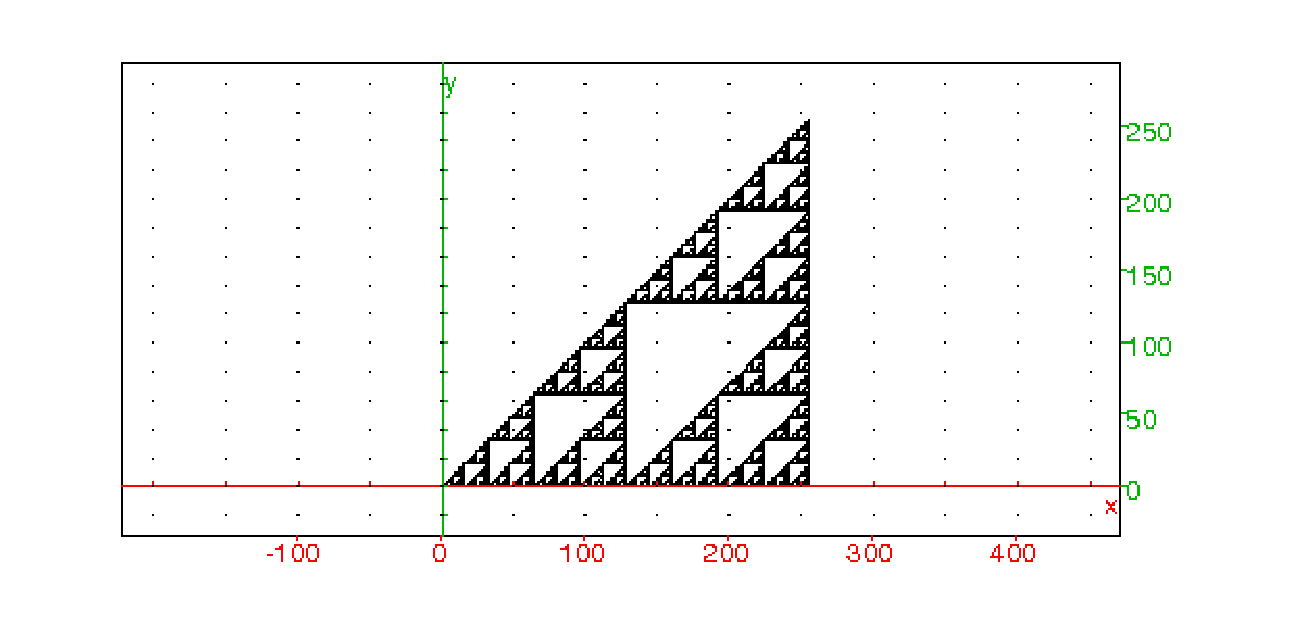
\includegraphics[width=\textwidth]{dessincomb}

\section{Un exercice}
On tire 100 fois de suite au hasard de fa\c{c}on \'equiprobable un entier $p$
parmi $1,2..100$ et on note $n_p$ le nombre de fois o\`u il a \'et\'e tir\'e.\\
\'Ecrire un programme qui repr\'esente les points $p,n_p$
On tape :
\begin{verbatim}
tirage():={
local p,np,j,L,P;
L:=0$(j=1..100)
pour j de 0 jusque 99 faire
p:=rand(100);
L[p]:=L[p]+1;
fpour;
P:=NULL;
pour p de 0 jusque 99 faire
np:=L[p];
si np!=0 alors P:=P,point(p+1+i*np); fsi; 
fpour;
print(max(L));
retourne P;
}:;
\end{verbatim}
On tape {\tt tirage()}\\
On obtient :

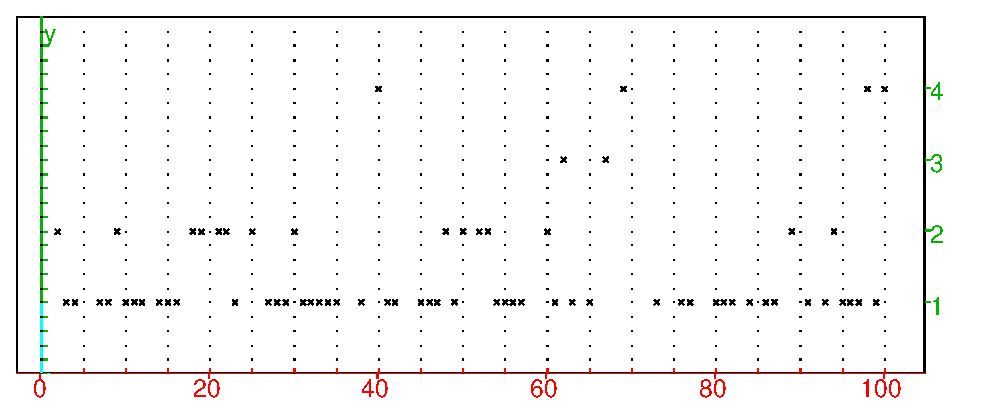
\includegraphics[width=\textwidth]{tirage}

\section{Valeur de $e$ et le hasard}
\subsection{L'\'enonc\'e}
On tire des nombres au hasard dans $[0;1[$ et on les ajoute. On s'arr\^ete quand
la somme obtenue est strictement plus grande que 1. On peut montrer que le 
nombres de tirages n\'ecessaires est en moyenne \'egal \`a $e$. \'Ecrire un 
programme v\'erifiant exp\'erimentalement ce r\'esultat.
\subsection{La solution avec {\tt Xcas}}
Dans {\tt Xcas}, on peut soit utiliser {\tt rand(0,1)}, soit utiliser  
la fonction {\tt f:=rand(0..1)} pour obtenir un nombre au hasard entre 0 et 1.\\
On tape :{\tt rand(0.1)}\\
On obtient : {\tt 0.482860322576}\\
On tape : {\tt f:=rand(0..1)}\\
puis : {\tt f()}
On obtient : {\tt 0.8627617261373}\\
puis : {\tt f()}
On obtient : {\tt 0.3095522336662} etc....\\
On \'ecrit le programme :
\begin{verbatim}
approxe(n):={
local j,S,k,N;
N:=0;
pour k de 1 jusque n faire
S:=0;
j:=0;
tantque S<=1 faire
S:=S+rand(0,1);
j:=j+1;
ftantque;
N:=N+j;
fpour;
retourne evalf(N/n);
}:;
\end{verbatim}
On tape : {\tt approxe(100000)}\\
On obtient : {\tt 2.71750000000}\\
 alors que {\tt evalf(e)=2.71828182846}
\section{Distance moyenne entre de 2 points}
\subsection{L'\'enonc\'e}
On veut \'evaluer la distance moyenne entre 2 points choisis au hasard :
dans un segment $S$ de longueur 1, dans le carr\'e unit\'e $C$ ou dans le cube 
unit\'e $K$.
\begin{enumerate}
\item \'Ecrire un programme qui calcule cette distance moyenne lorsque l'on 
choisit au hasard $n$ fois de suite 2 points dans $S$,dans $C$ ou dans $K$,
puis g\'en\'eraliser.
\item Faire une repr\'esentation graphique permettant de visualiser la 
r\'epartition des distances dans le cube unit\'e $K$.
\end{enumerate}
\subsection{La solution avec {\tt Xcas}}
\begin{enumerate}
\item
\begin{verbatim}
distS(n):={
local xa,xb,j,d,D;
D:=0;
pour j de 1 jusque n faire
xa:=rand(0,1);
xb:=rand(0,1);
d:=abs(xa-xb);
D:=D+d;
fpour;
retourne evalf(D/n);
}:;

distC(n):={
local xa,ya,xb,yb,j,d,D;
D:=0;
pour j de 1 jusque n faire
xa:=rand(0,1);ya:=rand(0,1);
xb:=rand(0,1);yb:=rand(0,1);
d:=distance([xa,ya],[xb,yb]);
D:=D+d;
fpour;
retourne evalf(D/n);
}:;

distK(n):={
local xa,ya,za,xb,yb,zb,j,d,D;
D:=0;
pour j de 1 jusque n faire
xa:=rand(0,1);ya:=rand(0,1);za:=rand(0,1);
xb:=rand(0,1);yb:=rand(0,1);zb:=rand(0,1);
d:=distance([xa,ya,za],[xb,yb,zb]);
D:=D+d;
fpour;
retourne evalf(D/n);
}:;

distp(p,n):={
local a,b,j,d,D;
D:=0;
pour j de 1 jusque n faire
a:=op(randMat(1,p,0..1));
b:=op(randMat(1,p,0..1));
d:=sqrt(sum((a-b)^2));
D:=D+d;
fpour;
retourne evalf(D/n);
}:;

\end{verbatim}
On tape : {\tt distS(100000)}\\
On obtient : {\tt 0.333424530881}\\
On tape : {\tt distC(100000)}\\
On obtient : {\tt 0.522140638365}\\
On tape : {\tt distK(100000)}\\
On obtient : {\tt 0.6627691590747}\\
On tape : {\tt distp(4,100000)}\\
On obtient : {\tt 0.777235961163}\\
On tape : {\tt distp(5,100000)}\\
On obtient : {\tt 0.877837288394}\\
\item
\begin{verbatim}
graphdist(n):={
local xa,ya,za,xb,yb,zb,j,d,L;
L:=NULL;
pour j de 1 jusque n faire
xa:=rand(0,1);ya:=rand(0,1);za:=rand(0,1);
xb:=rand(0,1);yb:=rand(0,1);zb:=rand(0,1);
d:=distance([xa,ya,za],[xb,yb,zb]);
L:=L,point(j+i*d);
fpour;
retourne L;
}:;
\end{verbatim}
\end{enumerate}
On tape : {\tt graphdist(10000)}\\
On obtient :

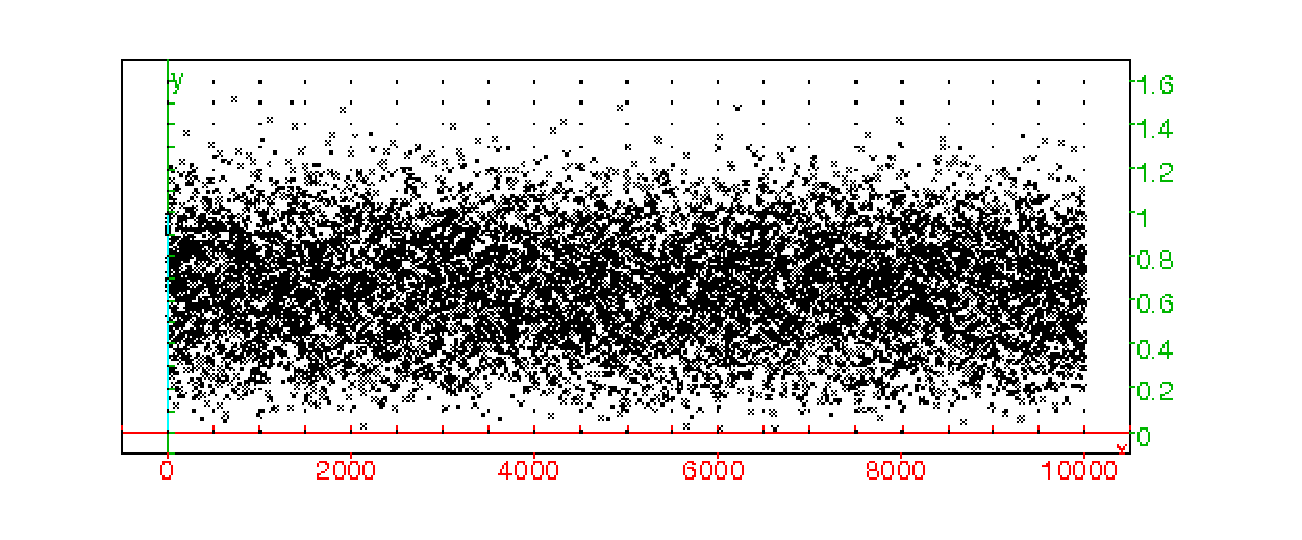
\includegraphics[width=\textwidth]{graphK}

\chapter{Les graphes et l'algorithme de Dijkstra}
Soit un graphe ayant $n$ sommets num\'erot\'es de 0 \`a $n-1$. Certains de ces 
sommets sont reli\'es par des ar\^etes de longueur donn\'ees.\\
L'algorithme de Dijkstra permet de trouver le chemin de distance minimale qui 
relie le sommet de num\'ero {\tt deb} aux autres sommets.\\
Cet algorithme proc\'ede de proche en proche en se servant de la remarque  :\\
si par exemple, le chemin le plus court pour aller du sommet 0 au sommet 2 
passe par le sommet 4, le d\'ebut de ce chemin est aussi le chemin le plus 
court pour aller du sommet 0 au sommet 4.\\
\section{L'algorithme sur un exemple}
Soient $n=4$ et le graphe de matrice {\tt A} :
$$
A=\left(\begin{array}{cccc}
0 & 27 & 11 & 23  \\
27 & 0 & 14 & 1 \\
11 & 14 & 0 & 10\\
23 & 1 & 10 & 0  
\end{array}\right)
$$
Je veux partir du sommet 0 pour aller au sommet 1 (resp 2,3) par le plus court 
chemin.\\
J'initialise :\\
{\tt dist} \`a {\tt [0,27,11,23]} (c'est \`a dire \`a la ligne 0 de {\tt A}) 
{\tt afaire} \`a {\tt [1,2,3]} et\\
{\tt sprec} \`a {\tt [-1,0,0,0]} ({\tt sprec[0]=-1} car on part du sommet 0 et 
pour {\tt j!=0}, {\tt sprec[j]=0} car {\tt dist} est la distance provisoire 
minimum pour aller de 0 \`a {\tt j}). Les 2 valeurs {\tt dist[0]} et 
{\tt sprec[0]} sont d\'efinitives car le sommet 0 est ici le d\'epart. Je sais
aussi que le chemin le plus court du sommet 0 au sommet 1 (resp 2,3) ne 
repassera pas par le sommet 0. \\
{\bf Premi\`ere \'etape}\\
Je cherche le minimum des valeurs de {\tt dist} pour les 
sommets dont les num\'eros sont dans {\tt afaire=[1,2,3]} c'est \`a dire le 
minimum de {\tt [27,11,23]}.\\
Le minimum 11 de {\tt [27,11,23]} est r\'ealis\'e pour le sommet 2 (car 
{\tt dist[2]=11}). Je supprime le num\'ero 2 de la liste {\tt afaire} qui 
devient {\tt afaire=[1,3]} car je connais maintenant
le plus court chemin pour aller de 0 \`a 2, il est direct
et a pour longueur 11 je ne change donc pas la valeur de {\tt dist[2]} ni celle de {\tt sprec[2]} : ces 2 valeurs sont maintenant d\'efinitives.\\
On a donc encore {\tt dist=[0,27,11,23]} et {\tt sprec=[-1,0,0,0]} o\`u les 
valeurs d'indice 0 et 2 sont d\'efinitives.\\
Maintenant, le chemin provisoirement le plus court allant du sommet 0 au sommet
1 (resp du sommet 0 au sommet 3) est :
\begin{itemize}
\item soit le chemin direct allant de 0 \`a 2, suivi par le chemin le plus 
court allant de 2 \`a 1 (resp de 2 \`a 3), 
\item soit le chemin le plus court allant de 0 \`a 1 (resp de 0 \`a 3) sans 
passer pas par 2.
\end{itemize}
L'\'etape suivante consiste donc \`a comparer le chemin le plus court de 0 \`a 
2 de longueur {\tt dist[2]}, suivi par le chemin direct de 2 \`a 1 de longueur
{\tt A[2,1]} (resp 3 de longueur {\tt A[2,3]}) avec le chemin le plus court 
provisoire qui va de 0 \`a 1 {\tt dist[1]} (respde 0 \`a 3 {\tt dist[3]}).\\
Je compare donc {\tt 27=dist[1]} \`a 11+14=25 (11={\tt dist[2]}=longueur du 
chemin minimum allant de 0 \`a 2 et {\tt 14=A[2,1]}=longueur du chemin direct 
allant de 2 \`a 1). On a 25<27 donc je modifie {\tt dist} en {\tt [0,25,11,23]} 
et {\tt sprec} en {\tt [-1,2,0,0]} puisque 25 est la longueur du chemin qui 
passe par 2.\\ 
Je compare donc {\tt 23=dist[3]} \`a 11+10=21 (11=longueur du chemin
minimum allant de 0 \`a 2 et {\tt 10=A[2,3]}=longueur du chemin direct allant 
de 2 \`a 3). On a 21<23 donc je modifie
{\tt dist} en {\tt [0,25,11,21]} et {\tt  sprec} en {\tt [-1,2,0,2]} puisque 21
 est la longueur du chemin qui passe par 2.\\ 
Donc maintenant {\tt dist=[0,25,11,21]} et {\tt  sprec=[-1,2,0,2]}\\
{\bf Deuxi\`eme \'etape}\\
Je cherche le minimum des valeurs de {\tt dist} pour les 
sommets de num\'eros {\tt afaire=[1,3]} c'est \`a dire le minimum de 
{\tt [25,21]}.\\
Le minimum 21 de {\tt [25,21]} est r\'ealis\'e pour le sommet 3 car 
{\tt dist[3]=21}. Je supprime le num\'ero 3 de la liste {\tt afaire} qui 
devient {\tt afaire=[1]} car je connais maintenant
le plus court chemin pour aller de 0 \`a 3, il est de 
longueur 21 et il passe par 2 car {\tt  sprec[3]=2}.\\
Je cherche enfin le plus court chemin pour aller de 0 \`a 1 en empruntant :
\begin{itemize}
\item soit le chemin minimum allant de 0 \`a 2 de longueur 11 (car 
{\tt dist[2]=11}), puis le chemin direct allant de 2 \`a 1 de longueur 
{\tt 14=A[2,1]} (donc un chemin de longueur 11+14=25={\tt dist[1]}), 
\item soit le chemin minimum qui va de 0 \`a 3  de longueur 21 (car 
{\tt dist[3]=21}), puis le chemin direct allant de 3 \`a 1  de longueur 
1=A[3,1] (donc un chemin de longueur 21+1=22).
\end{itemize} 
Je compare donc 25  \`a 22. On a 22<25 donc je modifie
{\tt dist} en {\tt [0,22,11,21]} et {\tt sprec} en {\tt [-1,3,0,2]}.\\
Donc maintenant {\tt dist=[0,22,11,21]} et {\tt  sprec=[-1,3,0,2]}\\
{\bf Troisi\`eme \'etape}\\
Il reste \`a chercher le minimum de {\tt [22]} est obtenu pour le sommet de 
num\'ero 1, num\'ero que l'on supprime de la liste {\tt afaire} qui devient 
vide.\\ 
Le r\'esultat final est donc :\\
{\tt dist=[0,22,11,21]} et {\tt sprec=[-1,3,0,2]}
\section{D\'escription de l'algorithme de Dijkstra}
Soit {\tt A} la matrice donnant la longueur des ar\^etes i.e. {\tt A[j,k]} est 
la longueur de l'ar\^ete reliant le sommet {\tt j} au sommet {\tt k} avec la 
convention de mettre {\tt A[j,k]=inf=}$+\infty$ quand il n'y a pas d'ar\^ete 
qui relie le sommet {\tt j} au sommet {\tt k}. \\
Soientt {\tt dist} un vecteur donnant les distances provisoires reliant le 
sommet de num\'ero {\tt deb} aux autres sommets et {\tt sprec[j]} le 
num\'ero du sommet pr\'ecedent {\tt j} par lequel on doit passer pour avoir la 
distance minimale provisoire.\\
 Par exemple si {\tt n=5} et si en fin de programme {\tt sprec=[3,2,0,-1,2]} 
cela veut dire que l'on part du sommet 3 car {\tt sprec[3]=-1}.\\
Si on cherche le plus court chemin pour aller du sommet 3 au sommet {\tt j=4} 
le chemin sera {\tt 3,???,4}. Mais comme {\tt sprec[4]=2} le chemin sera {\tt 3,??,2,4} puis, comme {\tt sprec[2]=0} et {\tt sprec[0]=3} le chemin sera 
{\tt 3,0,2,4}.\\
Par contre le chemin minimum pour aller du sommet {\tt 3} \`a {\tt 0}  sera 
direct de {\tt 3} \`a {\tt 0} puique {\tt sprec[0]=3}.\\
{\tt afaire} est la liste des indices restant \`a faire.\\
{\bf Initialisation :}\\
Au d\'ebut {\tt dist=A[deb]} ({\tt A[deb]} est la ligne d'indice {\tt deb} de 
{\tt A}) et \\
{\tt sprec[deb]=-1} et {\tt  sprec[j]=deb} pour {\tt j!:=deb}.\\
{\tt afaire} est la liste des indices dans laquelle on a enlev\'e {\tt deb} I.E. une liste de longueur {\tt n-1}.\\
{\bf Etapes suivantes :}\\
On cherche le minimum {\tt m} des distances provisoires {\tt dist} reliant le 
sommet {\tt deb} aux sommets dont les num\'eros sont dans 
{\tt afaire} et on note {\tt jm} le num\'ero du sommet r\'ealisant ce minimum.
On supprime {\tt jm} de la liste {\tt afaire}.\\
On compare ensuite, pour tous les num\'eros des sommets restant afaire, la 
longueur {\tt autredist} des chemins qui passent par 
{\tt jm} \`a la valeur provisoire {\tt dist} et si pour le sommet de num\'ero
{\tt k=afaire[j]} le chemin qui passe par {\tt jm} est plus court on modifie 
{\tt dist[k]} et on modifie {\tt sprec[k]} qui vaut alors {\tt jm}.\\
On recommence jusqu'a \'epuisement de la liste 
{\tt afaire} , c'est \`a dire que l'on fait cela {\tt n-1} fois.\\
{\bf Remarque}\\
 Attention aux indices !!!!\\
{\tt afaire} est la liste des indices ou num\'eros des 
sommets restant \`a traiter et il ne faut pas confondre le num\'ero des sommets 
et les indices qu'ils ont dans la liste {\tt afaire} i.e. ne pas confondre
{\tt k=afaire[j]} avec {\tt j} (si {\tt afaire=[2,0,1]} le sommet 0 a pour 
indice 1 dans {\tt afaire}).

\section{Le programme}
\begin{verbatim}
Dijkstra(A,deb):={
local j,k,n,na,dist,sprec,distaf,afaire,
      m,jm,autredist,jma;
// initialisation
n:=size(A);
dist:=A[deb];
sprec:=[deb $n];
sprec[deb]:=-1;
n:=n-1;
//afaire liste des indices restant a faire
afaire:=suppress([j$(j=0..n)],deb);
na:=size(afaire)-1;
pour k de 0 jusque n-1 faire 
//le sommet jm realise la dist m minimum de distaf
//jma est l'indice de m dans la liste distaf
//jm est l'indice de m dans la liste afaire 
distaf:=[dist[afaire[j]]$(j=0..na)];
m:=min(distaf);
//jma indice du minimum m dans afaire
jma:=member(m,distaf)-1;
//jm indice du minimum m dans dist
jm:=afaire[jma];
//fin prematuree
si m==inf alors return dist,sprec; fsi; 
afaire:=suppress(afaire,jma);
na:=na-1;
  pour j de 0 jusque na faire
     autredist:=m+A[jm,afaire[j]];
     si autredist<dist[afaire[j]] alors 
        dist[afaire[j]]:=autredist; 
        sprec[afaire[j]]:=jm;
     fsi;
  fpour; 
fpour;
retourne dist,sprec;
}:;
\end{verbatim}
On tape :\\
{\tt M:=[[0,27,11,23],[27,0,14,1],[11,14,0,10],[23,1,10,0]]}\\
{\tt Dijkstra(M,0)}\\
On obtient (cf la section pr\'ec\'edente) :\\
{\tt [0,22,11,21],[-1,3,0,2]}\\
On tape :\\
{\tt A:=[[0,1,6,7],[1,0,4,3],[6,4,0,1],[7,3,1,0]]}
{\tt Dijkstra(A,2)}\\
On obtient :\\
{\tt [5,4,0,1],[1,2,-1,2]}\\
cela veut dire par exemple pour aller de 2 \`a 0 la distance minimale est 5 et 
le chemin est 2,1,0.\\
On tape :\\
{\tt B:=[[0,1,6,7],[1,0,4,2],[6,4,0,1],[7,2,1,0]]}
{\tt Dijkstra(B,0)}\\
On obtient :\\
{\tt [0,1,4,3],[-1,0,3,1]}\\
cela veut dire par exemple pour aller de 0 \`a 2 la distance minimale est 4 et 
le chemin est 0,1,3,2.
\section{Le chemin le plus court d'un sommet \`a un autre}
On tape en utilisant le programme pr\'ec\'edent :
\begin{verbatim}
dijkstra2(A,deb,fin):={
local dist,sprec,long,chemin,j;
dist,sprec:=dijkstra(A,deb);
long:=dist[fin];
j:=sprec[fin];
chemin:=fin;
tantque j!=-1 faire 
chemin:=j,chemin;
j:=sprec[j];
ftantque;
retourne long,[chemin];
}:;
\end{verbatim}
ou bien en arr\'etant le programme d\`es que l'on a atteint le sommet {\tt fin},
on tape :
\begin{verbatim}
dijkstra3(A,deb,fin):={
local j,k,n,na,dist,sprec,distaf,afaire,m,
      jm,autred,jma,long,chemin;
n:=size(A);
//dist:=[inf$ n];dist[deb]:=0;
dist:=A[deb];
sprec:=[deb $n];
sprec[deb]:=-1;
n:=n-1;
//afaire liste des indices restant a faire
afaire:=suppress([j$(j=0..n)],deb);
na:=n-1;
pour k de 0 jusque n-1 faire
   //minimum des distances dist[afaire[j]]
   distaf:=[dist[afaire[j]]$(j=0..na)];
   m:=min(distaf);
   //jma indice du minimum m dans afaire
   jma:=member(m,distaf)-1;
   //jm indice du minimum m dans dist
   jm:=afaire[jma];
   si m==inf alors return dist,sprec; fsi;
   si jm==fin alors 
      long:=dist[fin];
      chemin:=jm;
      j:=sprec[jm];
      tantque j!=-1 faire 
        chemin:=j,chemin;
        j:=sprec[j];
      ftantque;
      retourne long,[chemin];
   fsi;
   afaire:=suppress(afaire,jma);
   na:=na-1;
   pour j de 0 jusque na faire
      autred:=m+A[jm,afaire[j]];
      si autred<dist[afaire[j]] alors  
         dist[afaire[j]]:=autred; 
         sprec[afaire[j]]:=jm; 
      fsi;
   fpour; 
fpour;
}:;
\end{verbatim}
On tape :\\
{\tt M:=[[0,27,11,23],[27,0,14,1],[11,14,0,10],[23,1,10,0]]}\\
{\tt dijkstra3(M,0,1)}\\
On obtient (cf la section pr\'ec\'edente) :\\
{\tt 22,[0,2,3,1]}\\
{\tt dijkstra3(M,0,2)}\\
On obtient (cf la section pr\'ec\'edente) :\\
{\tt 11,[0,2]}\\
{\tt dijkstra3(M,0,3)}\\
On obtient (cf la section pr\'ec\'edente) :\\
{\tt 21,[0,2,3]}\\
On tape :\\
{\tt A:=[[0,1,6,7],[1,0,4,3],[6,4,0,1],[7,3,1,0]]}\\
{\tt dijkstra2(A,2,0)} ou {\tt dijkstra3(A,2,0)}\\
On obtient : {\tt 5,[2,1,0]}\\
On tape :\\
{\tt B:=[[0,1,6,7],[1,0,4,2],[6,4,0,1],[7,2,1,0]]}\\
{\tt dijkstra2(B,0,2)} ou {\tt dijkstra3(B,0,2)}\\
On obtient :\\
{\tt 4,[0,1,3,2]}\\
On tape :\\
{\tt dijkstra2(B,2,0)} ou {\tt dijkstra3(B,2,0)}\\
On obtient :\\
{\tt 4,[2,3,1,0]}\\
{\bf Exemple avec une matrice cr\'eee al\'eatoirement}\\
On tape :\\
{\tt MR:=randmatrix(5,5,'alea(50)+1')}\\
{\tt M:=MR+tran(MR)}\\
{\tt pour j de 0 jusque 4 faire M[j,j]=<0; fpour;}\\
{\tt M}\\
On obtient :\\
{\tt [[0,47,91,57,60],[47,0,58,18,50],[91,58,0,22,74],}\\
{\tt [57,18,22,0,70],[60,50,74,70,0]]}\\
$$
\left(\begin{array}{ccccc}
0 & 47 & 91 & 57 & 60 \\
47 & 0 & 58 & 18 & 50 \\
91 & 58 & 0 & 22 & 74 \\
57 & 18 & 22  & 0 & 70 \\
60 & 50 & 74 & 70 & 0 
\end{array}\right)
$$
On tape :\\
{\tt Dijkstra(M,0)}\\
On obtient :\\
{\tt [0,47,79,57,60],[-1,0,3,0,0]}\\
On tape :\\
{\tt dijkstra2(M,0,2)}\\
On obtient :\\
{\tt 79,[0,3,2]}

\chapter{Exercices sur trigonom\'etrie et complexes}
\section{Les polyn\^omes de Tchebychev}
\subsection{L'\'enonc\'e}
Les polyn\^omes de Tchebychev $T_n$ sont tels que $\cos(nx)=T_n(\cos(x))$.\\
On a ainsi :\\
$T_0(x)=1$\\
$T_1(x)=x$\\
$T_2(x)=2x^2-1$\\
\begin{enumerate}
\item Montrer que pour $n\geq 1$ on a :\\
$T_{n+1}(x)=2xT_n(x)-T_{n-1}(x)$.
\item \'Ecrire une fonction de $n$ qui renvoie le polyn\^ome $T_n$, en utilisant
la relation $T_{n+1}(x)=2xT_n(x)-T_{n-1}(x)$.
\item \'Ecrire une fonction de $n$ qui renvoie le polyn\^ome $T_n$, en utilisant
les nombres complexes et la formule de Moivre.
\end{enumerate}
\subsection{La solution avec {\tt Xcas}}
Dans {\tt Xcas}, la fonction {\tt  tchebyshev1} qui renvoie le ni\`eme 
polyn\^ome de Tchebyshev de 1i\`ere esp\`ece existe. Cela va pouvoir permettre 
la v\'erification de vos programmes
\begin{enumerate}
\item La relation $T_{n+1}(x)=2xT_n(x)-T_{n-1}(x)$ est vraie pour $n=1$
car $T_2(x)=2xT_1(x)-T_0(x)=2x*x-2$
On a :
$\cos((n+1)x)=\cos(x)*\cos(nx)-\sin(x)*\sin(nx)$ et\\
$\cos((n-1)x)=\cos(x)*\cos(nx)+\sin(x)*\sin(nx)$\\
donc $\cos((n+1)x)+\cos((n-1)x)=2\cos(x)*\cos(nx)$\\
ou encore  $\cos((n+1)x)=2\cos(x)*\cos(nx)-\cos((n-1)x)$
c'est \`a dire :\\
$T_{n+1}(x)=2xT_n(x)-T_{n-1}(x)$
\item On \'ecrit une fonction {\tt Tcheb(n)} qui renvoie le polyn\^ome $T_n$, 
en utilisant la relation $T_{n+1}(x)=2xT_n(x)-T_{n-1}(x)$. :
\begin{verbatim}
Tcheb(n):={
local j,T0,T1,Tj;
T0:=1;
T1:=x;
pour j de 2 jusque n faire
Tj:=2*x*T1-T0;
T0:=T1;
T1:=Tj;
fpour;
return T1;
}:;
\end{verbatim}
On tape : {\tt Tcheb(7)}\\
On obtient :{\tt 64*x\verb|^|7-112*x\verb|^|5+56*x\verb|^|3-7*x}

\item On \'ecrit une fonction {\tt Tchebich(n)} qui renvoie le polyn\^ome $T_n$,
en utilisant la formule de Moivre ($\cos(nx)=re((\cos(x)+i\sin(x))^n)$) et 
l'\'egalit\'e $\sin(x)^2=1-\cos(x)^2$ :
\begin{verbatim}
Tchebich(n):={
local f;
f(x,y):=normal(re((x+i*y)^n));
return f(x,sqrt(1-x^2));
}:;
\end{verbatim}
On tape : {\tt Tchebich(7)}\\
On obtient :{\tt 64*x\verb|^|7-112*x\verb|^|5+56*x\verb|^|3-7*x}\\

{\bf Remarque}\\
On peut v\'erifier car cette fontion existe dans {\tt Xcas}, on tape 
On tape : {\tt tchebyshev1(7)}\\
On obtient :{\tt 64*x\verb|^|7-112*x\verb|^|5+56*x\verb|^|3-7*x}
\end{enumerate}

\chapter{Codage}
\section{Codage de Jules Cesar}\label{sec:Cesar}
\subsection{Introduction}
Le principe est simple : on \'ecrit un message en n'utilisant que les 26 
lettres de l'alphabet et on le code en remplacant une lettre par une autre 
lettre.
 Ceci peut \^etre consid\'er\'e comme une  application $f$ de l'ensemble 
des lettres \{A,B,C,...X,Y,Z\}  dans lui-m\^eme.\\ 
Pour pouvoir d\'ecoder, il faut que l'application $f$ ci-dessus soit 
bijective!\\
Il parait que Jules C\'esar utilisait cette m\'ethode pour communiquer ses 
ordres.
\subsection{Codage par sym\'etrie point ou par rotation d'angle $\pi$}\label{sec:symp}
Une fa\c{c}on simple de coder est la suivante :\\
on \'ecrit les lettres sur un cercle (de fa\c{c}on \'equir\'epartie) et on 
remplace chaque lettre par la lettre sym\'etrique par rapport au centre du 
cercle :

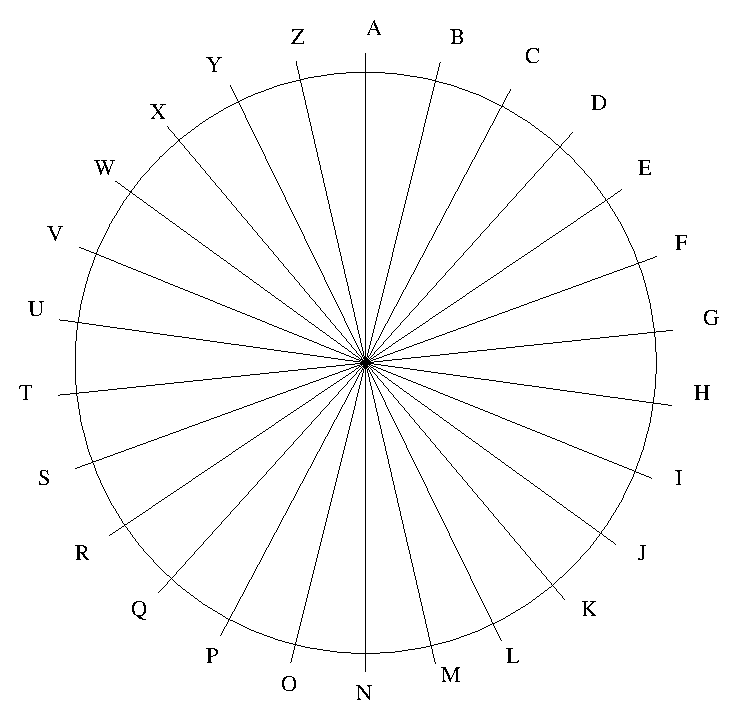
\includegraphics[width=9cm]{codage}

Le d\'ecodage s'obtient de la m\^eme fa\c{c}on car ici $f \circ f=Id$ 

\subsection{Avec les \'el\`eves}
On explique que l'on va coder un message en remplacant une lettre par une autre
(on suppose que le message n'utilise que les 26 lettres de l'alphabet et que 
l'on n'\'ecrit pas les espaces). \\
Pour cela on distribue une feuille sur laquelle figure quatre cercles divis\'es
en 26 parties \'egales.\\
 On \'ecrit sur ce cercle les 26 lettres de l'alphabet et le codage consiste 
\`a remplacer chaque lettre du message par la lettre diam\'etralement oppos\'eesur le cercle.\\
Par exemple voici le message \`a coder selon cette m\'ethode :\\
"BONJOURLESAMIS"\\
Le  message \`a d\'ecoder est donc :\\
"OBAWBHEYRFNZVF"\\
Quel sont les \'el\'ements pertinents qu'il faut transmettre pour que le
d\'ecodage soit possible ?\\
Parmi les r\'eponses il est apparu qu'il fallait ajouter $+13$ pour d\'ecoder.\\
Puis chaque \'el\`eve invente un codage et \'ecrit un message  selon son codage
 et le donne \`a d\'ecoder  \`a son voisin, par \'ecrit avec les explications 
n\'ecessaires pour le d\'ecoder.\\
Voici quelques codages obtenus :\\
- codage obtenu en remplacant chaque lettre par celle qui la suit dans 
l'alphabet,\\
- codage obtenu en remplacant chaque lettre par celle qui est obtenue en 
avan\c{c}ant de +4 sur la roue (ou en reculant de 3 etc...),\\
- codage obtenu  en rempla\c{c}ant chaque lettre par celle qui est obtenue
par sym\'etrie par rapport \`a la droite [A,N] (verticale sur le dessin),ou par 
sym\'etrie par rapport \`a la droite horizontale sur le dessin,\\
- codage par sym\'etrie par rapport au centre du cercle mais o\`u l'ordre des 
lettres sur le cercle n'est pas respect\'e,\\
- d'autres codages comme de remplacer le message par une suite de nombres 
(int\'eressant mais cela ne repond pas \`a la question pos\'ee),\\
- codage qui d\'epend de la position de la lettre dans le message. Ce codage
n'est pas une application puisque une m\^eme lettre peut avoir des codages 
diff\'erents.\\
Combien y-a-t-il de codages (i.e de bijections) possibles ?\\
Il a fallut parler de bijections :\\
un \'etudiant a dit qu'il fallait que deux lettres diff\'erentes soient cod\'ees par
 des lettres diff\'erentes pour que le d\'ecodage soit possible (injection).\\
Ceci entraine que toutes les lettres sont le codage d'une autre lettre
 (surjection).\\
Pour simplifier on a pr\'ef\'er\'e parler de permutations des lettres avec comme
exemple : trouver tous les codages possibles si on suppose que l'alphabet 
 utilis\'e ne comporte que les trois lettres A, B, C.\\
Donnez un ordre de grandeur de 26!\\
A supposer que vous vouliez \'ecrire les  26! codages possibles sur un cahier et
que votre rythme est de 1 codage par seconde (vous \^etes super rapide !!!...
f\'elicitations !!!) combien de temps (r\'eponse en heures, en mois, en ann\'ees...?) 
 vous faut-il ?\\ 
Combien de cahiers de 10000 lignes (200  pages de 50 lignes) vous faut-il ? 
Donner la longueur occup\'ee par ces cahiers dans une biblioth\`eque, si chaque
 cahier occupe 1 cm. 
Combien y-a-t-il de codages involutifs possibles qui sont sans point double 
(c'est \`a dire de bijections $f$
v\'erifiant $f=f^{-1}$ et $f(x)\neq x $ pour tout $x$)  ?\\
Comment faire pour que la cl\'e du d\'ecodage soit simple ?
\subsection{Travail dans  Z/26Z}
Le codage de Jules C\'esar consiste \`a faire une sym\'etrie point ou encore 
une rotation d'angle $\pi$.\\
Si on num\'erote les lettres de 0 \`a 25, le codage consiste  donc \`a faire 
une addition de 13 (modulo 26). 
(voir figure \ref{sec:symp}).\\
{\bf Exemple}  :\\
"BONJOUR" sera cod\'e par "OBAWBHE"

\subsection{Codage par  rotation d'angle $\alpha=k*\pi/13$}\label{sec:rotn}
Le principe est le m\^eme :\\
on \'ecrit les lettres sur un cercle (de fa\c{c}on \'equir\'epartie) et on remplace 
chaque lettre par la lettre obtenue par rotation d'angle 
$\alpha=k*\pi/13\ (0\leq \ k\ \leq \ 25)$ (k est un entier).\\
Si on num\'erote les lettres de 0 \`a 25,  le codage consiste  donc \`a faire subir
\`a chaque lettre un d\'ecalage de {\tt k} c'est \`a dire \`a faire subir \`a son 
num\'ero une addition de {\tt k} (modulo 26) (voir figure \ref{sec:rotn}).\\
On remarquera que si le param\`etre de codage par rotation est {\tt k}, le 
d\'ecodage sera un codage par rotation  de param\`etre {\tt -k} ou encore
 {\tt 26-k}.

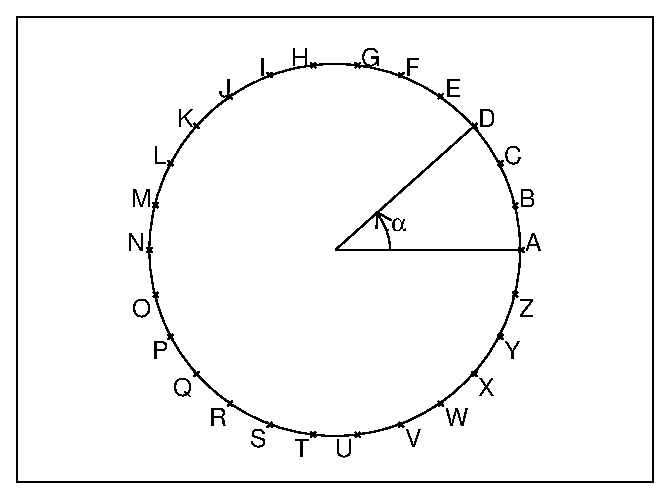
\includegraphics[width=9cm]{codrot}
%\begin{figure}[h t p d]
%\centering\includegraphics{rot.eps}
%\caption{Codage par rotation de $5*\pi/13$}\label{sec:rotn}
%\end{figure}
\section{\'Ecriture des programmes correspondants}
\subsection{Passage d'une lettre \`a un entier entre  0 et 25}\index{asc}
\`A chaque lettre on peut faire correspondre son code ASCII.\\
Avec {\tt Xcas}, {\tt asc("A")=[65]} et {\tt asc("BON")=[66,79,78]}.\\
 Donc pour avoir un entier entre 
0 et 25 il suffit de retrancher 65 :\\
 {\tt asc("A")-65} ({\tt =0}) ou {\tt asc("BON")-[65,65,65]} ({\tt =[1,14,13]}).\\
On \'ecrit donc la proc\'edure {\tt c2n} qui transforme une cha\^{\i}ne de caract\`eres 
{\tt m} en une liste d'entiers {\tt l=c2n(m)} entre 0 et 25 (le 2 de {\tt c2n} veut dire "to" ou "vers" en fran\c{c}ais).\\
Il faut cr\'eer une liste form\'ee des nombres {\tt 65} et de m\^eme longueur que le message avec {\tt makelist(65,1,size(m))}.\\
On \'ecrit :
\begin{verbatim}
c2n(m):={
return(asc(m)-makelist(65,1,size(m)));
}
\end{verbatim}
{\bf Exemple} :\\
{\tt c2n("BONJOUR")=[1,14,13,9,14,20,17]}
\subsection{Passage d'un entier entre  0 et 25 \`a une lettre}\index{char}
\`A chaque entier $n$ compris entre 0 et 25, on fait correspondre la 
$(n-1)^{ieme}$ lettre  en majuscule de l'alphabet (\`a 0 correspond "A", 
`a 1 correspond "B" etc...).\\
Avec {\tt Xcas}, {\tt char(65)="A"} et {\tt char([66,79,78])="BON"}.\\
On \'ecrit donc la proc\'edure {\tt n2c} qui transforme une liste d'entiers 
{\tt l}
entre 0 et 25 en une cha\^{\i}ne de caract\`eres {\tt m}.\\ 
Il faut penser \`a ajouter {\tt 65} \`a tous les \'el\'ements de la liste 
{\tt l} (on forme une liste form\'ee de {\tt 65} avec la fonction 
{\tt makelist} :
{\tt l+makelist(65,1,size(l))}).\\
On \'ecrit :
\begin{verbatim}
n2c(l):={
return(char(l+makelist(65,1,size(l))));
}
\end{verbatim}

{\bf Exemple} :\\
{\tt n2c([1,14,13,9,14,20,17])="BONJOUR"} 
\subsection{Passage d'un entier k entre  0 et 25 \`a l'entier n+k mod 26}
On \'ecrit donc la proc\'edure {\tt decal} de param\`etres {\tt n} et {\tt l} qui 
transforme une liste {\tt l} d'entiers  {\tt k} entre 0 et 25 en la liste d'entiers 
${\tt n+k \ mod\ 26}$.\\
On \'ecrit :
\begin{verbatim}
decal(n,l):={
return(irem(l+makelist(n,1,size(l)),26));
}
\end{verbatim}
{\bf Exemple} :\\
{\tt decal(13,[1,14,13,9,14,20,17])=[14,1,0,22,1,7,4]}
\subsection{Codage d'un message selon Jules C\'esar}
On \'ecrit la proc\'edure finale {\tt CESAR} qui a deux param\`etres :\\
l'entier {\tt n} de d\'ecalage et le message {\tt m}.\\
On \'ecrit :
\begin{verbatim}
cesar(n,m):={
return(n2c(decal(n,c2n(m))));
}
\end{verbatim}
{\bf Exemple} :\\
{\tt cesar(13,"BONJOUR")="OBAWBHE"}
\section{Codage en utilisant une sym\'etrie par rapport \`a un axe} 
\begin{figure}[h t p d]
\centering
%\includegraphics{sy.eps}
\caption{Codage par sym\'etrie par rapport \`a Ox}\label{sec:symd}
\end{figure}
\subsection{Passage d'un entier k entre  0 et 25 \`a l'entier n-k mod 26}
On reprend les proc\'edures {\tt c2n} et {\tt n2c} vues pr\'ec\'edemment :\\
{\tt c2n} transforme une cha\^{\i}ne
 de caract\`eres {\tt m} en  une liste d'entiers entre 0 et 25 et {\tt n2c} 
 transforme une liste {\tt l} d'entiers entre
0 et 25 en  une cha\^{\i}ne de caract\`eres {\tt m}.\\ 
On \'ecrit ensuite la proc\'edure {\tt sym} de param\`etres {\tt n} et {\tt l} qui
transforme une liste  {\tt l} d'entiers {\tt k} entre 0 et 25 en la liste 
d'entiers ${\tt n-k\ mod\ 26}$.
On peut consid\'erer que le param\`etre {\tt n} d\'etermine le diam\`etre {\tt D}
perpendiculaire \`a la corde {\tt [0,n]} (joignant {\tt A} \`a la {\tt (n-1)i\`eme} lettre).\\
La proc\'edure  {\tt sym} de param\`etre 
{\tt n} est donc  une sym\'etrie par rapport \`a la droite {\tt D}.\\
On \'ecrit :
\begin{verbatim}
sym(n,l):={
return(irem(makelist(n,1,size(l))-l,26));
}
\end{verbatim}

\subsection{Codage d'un message selon une sym\'etrie droite D}
On \'ecrit la proc\'edure finale {\tt cesarsym} qui a deux param\`etres :\\
l'entier {\tt n} (d\'efinissant la corde {\tt [0,n]} normale au diam\`etre {\tt D})
  et le message {\tt m}.\\
On \'ecrit :
\begin{verbatim}
cesarsym(n,m):={
return(n2c(sym(n,c2n(m))));
}
\end{verbatim}
{\bf Exemple} :\\
Si on prend {\tt n=13} on r\'ealise une sym\'etrie par rapport \`a la droite {\tt Ox}
(cf figure \ref{sec:symd}).\\
{\tt cesarsym(13,"BONJOUR")="MZAEZTW"}
\section{Codage en utilisant une application affine}
Comme pr\'ec\'edemment, on \'ecrit la proc\'edure {\tt c2n} qui transforme une cha\^{\i}ne
 de caract\`eres {\tt m} en  une liste d'entiers entre 0 et 25 et on \'ecrit 
la proc\'edure {\tt n2c} qui transforme une liste {\tt l} d'entiers entre 
0 et 25 en  une cha\^{\i}ne de caract\`eres {\tt m}.\\ 
On \'ecrit ensuite la proc\'edure {\tt affine} de param\`etre {\tt a,b,l} qui
transforme une liste  {\tt l} d'entiers {\tt k} entre 0 et 25 en la liste 
d'entiers ${\tt a*k+b\ mod\ 26}$.\\
On \'ecrit :
\begin{verbatim}
affine(a,b,l):={
return(irem((a*l+makelist(b,1,size(l))),26));
}
\end{verbatim}
On \'ecrit ensuite :
\begin{verbatim}
cesaraffine(a,b,m):={
return(n2c(affine(a,b,c2n(m))));
}
\end{verbatim}
Question :\\
Pour quelles valeurs de $a$ et $b$ le codage obtenu par {\tt cesaraffine} peut-il \^etre d\'ecod\'e ?

\section{Codage en utilisant un groupement de deux lettres}
On \'ecrit la proc\'edure {\tt c2n2} qui transforme une cha\^{\i}ne de caract\`eres
 {\tt m} en  une liste {\tt l} d'entiers entre 0 et $26^2-1=675$ :\\
On fait des groupements de deux lettres (quitte \`a terminer le message par la 
lettre "F" pour avoir un nombre pair de lettres), chaque groupement est
consid\'er\'e comme l'\'ecriture en base 26 d'un entier en utilisant comme 
"chiffre" les lettres majuscules. Ainsi, {\tt "BC"} est l'\'ecriture en base 26 de 28 (28=1*26+2).  \\
On \'ecrit :
\begin{verbatim}
c2n2(m):={
local s,lr,l,n;
s:=size(m);
if (irem(s,2)==1){
m:=append(m,"F");
s:=s+1;
}
lr:=[];
l:=asc(m);
for (k:=0;k<s;k:=k+2){
n:=l[k]*26+l[k+1];
lr:=append(lr,n);
}
return(lr);
}
\end{verbatim}

On \'ecrit ensuite la proc\'edure {\tt n2c2} qui transforme une liste 
d'entiers 
entre 0 et 675 (675=25*26+25=26*26-1) en une cha\^{\i}ne de caract\`eres 
{\tt m} :\\
chaque entier \'etant \'ecrit en base 26 avec comme "symboles" les 26 lettres 
majuscules.\\
On \'ecrit :
\begin{verbatim}
n2c2(l):={
local s,n,m;
s:=size(l);
m:="";
for (k:=0;k<s;k++){
n:=l[k];
m:=append(m,char(iquo(n,26)+65));
m:=append(m,char(irem(n,26)+65));
}
return(m);
}
\end{verbatim}
 On \'ecrit ensuite la fonction {\tt affin2} de param\`etre {\tt a,b,l} qui
transforme une liste  {\tt l} d'entiers {\tt k} entre 0 et 675 en la liste 
d'entiers ${\tt a*k+b\ mod\ 676}$ (entiers encore compris entre 0 et 675).\\
On \'ecrit :
\begin{verbatim}
affin2(a,b,l):={
local s;
s:=size(l);
for (k:=0;k<s;k++){
l[k]:=irem(a*l[k]+b,676);
}
return(l);
}
\end{verbatim}
On \'ecrit ensuite la fonction {\tt cesar2} qui r\'ealise le codage par 
groupement de 2 lettres utilisant l'application affine {\tt affin2}:
\begin{verbatim}
cesar2(a,b,m):={
return(n2c2(affin2(a,b,c2n2(m))));
}
\end{verbatim}
{\bf Question} :\\
Pour quelles valeurs $a1$ de $a$ et $b1$ de $b$, le codage obtenu par 
{\tt cesaraffine} peut-il \^etre d\'ecod\'e ?\\
{\bf R\'eponse} :\\
On doit avoir $a1*(a*n+b)+b1=a1*a*n+a1*b+b1=n$.\\
Il suffit donc de prendre : $b1=-a1*b \bmod 676$ et $a1*a=1 \bmod 676$
\section{Le codage Jules C\'esar et le codage lin\'eaire} 
\subsection{Les caract\`eres et leurs codes}\label{sec:code}
Ici, on ne se borne plus aux 26 lettres de l'alphabet, mais on veut pouvoir 
 utiliser les  101 caract\`eres de la table ci-dessous.\\
Dans cette table, on a le code du caract\`ere, puis, le caract\`ere : ainsi
"5" a pour code 21 et "R" a pour code 50 et l'espace " " a pour code 0.\\
\ \\

\begin{tabular}{|l|l|l|l|l|l|l|l|l|l|}
\hline
\ 0  &&&&&&&&&\\
\ 1~ ! &\ 2~ " &\ 3 \# &\ 4 \$ &\ 5 \% &\ 6 \& &\ 7~ ' &\ 8 ( &\ 9 ) &10 * \\
11 + &12 , &13 - &14 . &15 / &16 0 &17 1 &18 2 &19 3 &20 4 \\
21 5 &22 6 &23 7 &24 8 &25 9 &26 : &27~ ; &28 < &29 = &30 > \\
31 ? &32 @ &33 A &34 B &35 C &36 D &37 E &38 F &39 G &40 H \\
41 I &42 J &43 K &44 L &45 M &46 N &47 O &48 P &49 Q &50 R \\
51 S &52 T &53 U &54 V &55 W &56 X &57 Y &58 Z &59 [ &60 $\backslash$ \\
61 ] &62 \^ &63 \_ &64 ` &65 a &66 b &67 c &68 d &69 e &70 f \\
71 g &72 h &73 i &74 j &75 k &76 l &77 m &78 n &79 o &80 p \\
81 q &82 r &83 s &84 t &85 u &86 v &87 w &88 x &89 y &90 z \\
91 \{ &92 | &93 \} &94 \~ &95 \^e &96 \`u &97 \c{c} &98 \`a &99 \`e &100 \'e \\
\hline
\end{tabular}\\
\subsection{Les diff\'erentes \'etapes du codage}
Voici les diff\'erentes \'etapes du codage (elles seront programm\'ees avec 
{\tt Xcas} dans le paragraphe suivant) :
\begin{enumerate}
\item \`A chaque lettre ou symbole,
on associe un nombre, comme dans la table \ref{sec:code}. Un texte devient ainsi 
une suite de nombres~: par exemple {\tt \^e} sera cod\'ee par 95 et
{\tt BONJOUR} par 34 47 46 42 47 53 50.\\
La fonction {\tt codec2n} r\'ealise cette \'etape : elle transforme un 
caract\`ere en un nombre $n$ ($0 \leq n< 101$), selon la table \ref{sec:code}.
\item On effectue une ou plusieurs op\'erations sur ces nombres~:
\begin{itemize}
\item pour le codage de Jules C\'esar, on ajoute \`a ces nombres un nombre 
fix\'e appel\'e clef de chiffrement (par exemple 17), puis on prend le 
reste de la division par 101 des nombres obtenus.
Ainsi avec ce codage, {\tt \^e} est transform\'e 95
qui  est transform\'e en 11 (95+17=112 =101+11, ou encore, 11 est le reste 
de la division de 112 par 101).\\
Avec {\tt Xcas}, on effectue la transformation de {\tt n} avec la commande 
{\tt irem(n+clef,101)}, o\`u {\tt clef} est une variable qui contient la clef 
de chiffrement.  
\item pour le codage lin\'eaire on multiplie ces nombres par un nombre 
fix\'e  appel\'e clef de chiffrement (par exemple 17) puis on prend le reste de la division par 101 des nombres obtenus.
Ainsi avec ce codage {\tt \^e} est transform\'e 95 qui est 
transform\'e en 100 (95*17=1615 =15*101+100, ou encore, 100 est le reste de la
division de 1615 par 101).\\
Avec {\tt Xcas},  on effectue la transformation de {\tt n} avec la commande :\\
{\tt irem(n*clef,101)}\\
 si {\tt clef} est une variable qui contient la clef de chiffrement.
\end{itemize}
\item On transforme ensuite cette suite de nombre en une suite de caract\`eres,
 c'est le message crypt\'e. 
Ainsi, avec le codage de Jules C\'esar de clef 17, {\tt \^e} devient 
{\tt +} et {\tt BONJOUR} devient 
{\tt S`\_|`fc} et 
avec le codage lin\'eaire de clef 17, {\tt \^e} devient 
{\tt \'e} et {\tt BONJOUR} devient 
{\tt i|k'|\}J}.\\
La fonction {\tt coden2c} r\'ealise cette \'etape : elle transforme un nombre 
$n$ ($0 \leq n< 101$) en un caract\`ere $c$, selon la table \ref{sec:code}.
\item Le d\'ecryptage n\'ecessite d'inverser les op\'erations 3, 2 et 1.
Dans les exemples~:
\begin{itemize}
\item avec le codage de Jules C\'esar, il faut enlever 17 ou rajouter 84
et prendre le reste de la division par 101, 
(84 est la clef de d\'echiffrement car 84+17=101). Ainsi, 11 est d\'ecript\'e par
 95 puisque 11+84=95.
\item avec le codage lin\'eaire, il faut multiplier par 6 et prendre 
le reste de la division par 101, (6 est la clef de d\'echiffrement car 
6*17=102=101+1). Ainsi, 100 est d\'ecript\'e par 95 puisque 100*6=5*101+95.
\end{itemize} 
Le calcul de la
clef de d\'echiffrement \`a partir de la clef de chiffrement
fait intervenir l'arithm\'etique des entiers :\\
- savoir trouver l'oppos\'e $u$ d'un \'el\'ement $n$ de $Z/101Z$  pour le 
codage de Jules C\'esar ($u=101-n$ car $u+n=101$).\\
- savoir utiliser l'identit\'e de B\'ezout pour trouver l'inverse $u$
d'un \'el\'ement de $n$ de $Z/101Z$ pour le codage lin\'eaire (on a
$u={\tt iegcd(n,101)[0]}$ car   $u*n+v*101=1$).
\end{enumerate}
\subsection{Le programme Xcas}

\begin{verbatim}
codec2n(c):={
if (c=="\'e") return 100;
if (c=="\`e") return 99;
if (c=="\`a") return 98;
if (c=="\c{c}") return 97;
if (c=="\`u") return 96;
if (c=="\^e") return 95;
return(asc(c)-32);
};

coden2c(k):={
if (k== 100) return "\'e";
if (k==99) return "\`e";
if (k==98) return "\`a";
if (k==97) return "\c{c}";
if (k==96) return "\`u";
if (k==95) return "\^e";
return(char(k+32));
};

jules_cesar(message,clef):={
local s,j,messcode;
s:=size(message);
messcode:="";
for (j:=0;j<s;j++) {
messcode:=append(messcode,
                 coden2c(irem(clef+codec2n(message[j]),101)));
}
return (messcode);
};

lineaire(message,clef):={
local s,j,messcode;
s:=size(message);
messcode:="";
for (j:=0;j<s;j++) {
messcode:=messcode+coden2c(irem(clef*codec2n(message[j]),101));
}
return (messcode);
};
\end{verbatim}

{\tt codec2n} transforme un caract\`ere $c$ "autoris\'e" en un entier $n$, 
$0\leq n <101$ selon la table \ref{sec:code}.\\
{\tt coden2c} transforme un entier $n$, $0\leq n <101$ 
en un caract\`ere $c$ selon la table \ref{sec:code}.\\
{\tt jules\_cesar} (respectivement {\tt lineaire}) code le message selon la 
cl\'e choisie. On remarquera que les deux fonctions ne diff\`erent que par 
l'op\'eration effectu\'ee :\\
{\tt clef+codec2n(message[j])} pour la fonction {\tt jules\_cesar} et \\
{\tt clef+codec2n(message[j])} pour la fonction {\tt lineaire}.\\
Pour d\'ecoder, il suffit d'employer le m\^eme programme en utilisant la clef 
de d\'ecodage associ\'ee \`a la clef de codage et \`a la m\'ethode utilis\'ee :
par exemple, pour  {\tt jules\_cesar} de clef de codage 99 la cl\'e 
de d\'ecodage associ\'ee est 2 ($2+99=101=0 \bmod 101$) et \\
pour  {\tt lineaire} de clef de codage 99 la clef 
de d\'ecodage associ\'ee est 50 puisque $99*50=-2*50=-100=1 \bmod 101$.


\subsection{Le programme C++}
\begin{verbatim}
//#include <iostream>
#include <stdio.h>
#include <string.h>
#include <stdlib.h>

//using namespace std;

int codec2n(char c){
  int i=c;
  switch (c){
  case  '\'e':
    i=100; 
    break;
  case '\`e':
    i=99;
    break;
  case '\`a':
    i=98;
    break;
  case '\c{c}':
    i=97;
    break;
  case '\`u':
    i=96;
    break;
  case '\^e':
    i=95;
    break;
  default:
    i -= 32;
  }
  return i;
}

char coden2c(int i){
  if (i<95)
    return i+32;
  switch (i){
  case 95:
    return '\^e';
  case 96:
    return '\`u';
  case 97:
    return '\c{c}';
  case 98:
    return '\`a';
  case 99:
    return '\`e';
  case 100:
    return '\'e';
  }
}

int main(int argc,char ** argv){
  char * s=0,ch;
  size_t n=0;
  int i,d,fois;
  if (!strcmp(argv[0],"./table")){
    for (i=0;i<101;++i){
      ch=coden2c(i);
      printf("%d:%c &",i,ch);
      if (i%10==0)
	printf("\n");
    }
    return 0;
  }
  if (!strcmp(argv[0],"./coden2c")){
    for (i=1;i<argc;++i){
      d=atoi(argv[i]);
      ch=coden2c(d);
      printf("%c",ch);
    }
    printf("\n");
    return 0;
  }
  if (argc==3)
    fois=atoi(argv[2]);
  else
    fois=0;
  if (argc>=2){
    s=argv[1];
    n=strlen(s);
  }
  else {
    printf("Entrez un message \`a num\'eriser\n");
    getline(&s,&n,stdin);
    n=strlen(s)-1;
  }
  for (i=0;i<n;++i){
    d=codec2n(s[i]);
    if (fois)
      printf("%c",coden2c(d*fois % 101));
    else
      printf("%d ",d);
  }
  printf("\n");
  return 0;
}
\end{verbatim}
\subsection{Exercices de d\'ecodage}
\subsubsection{Avec le codage Jules C\'esar}
{\Large

message 1, codage Jules C\'esar clef 10\\
\verb_\`uy\^e}*kvvo\'e*qkqxo|*\^ex*MN_

\vspace{1cm}

message 2, codage Jules C\'esar clef 10\\
\verb|vk*}yv\^e~syx*x1o}~*zk}*)\`usnox~o|

\vspace{1cm}

message 3, codage Jules C\'esar clef 23\\
\verb_(\`u(|7\`e|%7\`e!~\`uz\`u|\`e%7\`e\`uy$|%_

\vspace{1cm}

message 4, codage Jules C\'esar clef 23\\
\verb_$\`u| 7 |7%|$&7{|7z!'$\`u$_

\vspace{1cm}

message 5, codage Jules C\'esar clef 35\\
\verb_\'e..#*-,1C3,C!&\'e2C3,C!&\'e2_

\vspace{1cm}

message 6, codage Jules C\'esar clef 35\\
{\tt *\'eC0B.-,1\#C0\#*A4\#C"3C"B\$'}
\vspace{1cm}

message 7, codage Jules C\'esar clef 99\\
\verb|f_`gjcr\`aq\`ea_jasj_rmgpcq\`em`jge_rmgpcq|

\vspace{1cm}

message 8, codage Jules C\'esar clef 99\\
\verb|gj\`ed_gr\`e`c_s\`ecr\`eaf_sb|

\vspace{1cm}

message 9, codage Jules C\'esar clef 51\\
\verb_:ZCB7:7A/B7=<S23S13S1=2/53S3ABS27A1CB/0:3_

\vspace{1cm}

message 10, codage Jules C\'esar clef 51\\
\verb_<=CASD=C:=<ASRD7B3@S:/S1=<4CA7=<_

\vspace{1cm}
message 11, codage Jules C\'esar clef 45\\
\verb|*-)=+7=8M,-M<:)>)14M87=:M:1-6|

\vspace{1cm}

message 12, codage Jules C\'esar clef 45\\
\verb|;+1-6+-M;)6;M+76;+1-6+-M6T-;<M9=-M:=16-M,-M4T)5-|
}
\subsubsection{Avec le codage lin\'eaire}
{\Large
message 1, codage lin\'eaire clef 10\\
%{\tt TsJ6 LUUt| \#L\#it, Ji OY}\\
\verb_TsJ6 LUUt| #L#it, Ji OY_
\vspace{1cm}

message 2, codage lin\'eaire clef 10\\
\verb|UL 6sUJ@7si ift6@ }L6 {T7jti@t|

\vspace{1cm}

message 3, codage lin\'eaire clef 23\\
%{\tt [\_[h\hspace{0.5em} ?h\{ \hspace{0.5em}?\'e1\_\hspace{-0.5em}:\_h?\{\hspace{0.5em} ?\_\#dh\{}\\
\verb|[_[h ?h{ ?\'e1_:_h?{ ?_#dh{|
\vspace{1cm}

message 4, codage lin\'eaire clef 23\\
\verb|d_hm mh {hd- Qh :\'eDd_d|

\vspace{1cm}

message 5, codage lin\'eaire clef 35\\
%{\tt Uii|BF\#m N\# 6\`uU+ N\# 6\`uU+}\\
\verb_Uii|BF#m N# 6\`uU+ N# 6\`uU+_
\vspace{1cm}

message 6, codage lin\'eaire clef 35\\
%{\tt BU JbiF\#m| J|B?q| YN Yb:>}\\
\verb_ BU JbiF#m| J|B?q| YN Yb:>_
\vspace{1cm}

message 7, codage lin\'eaire clef 99\\
\verb|ZhfXR`B"D dhRd@RhBLXF`D LfRX\hBLXF`D|

\vspace{1cm}

message 8, codage lin\'eaire clef 99\\
\verb|XR ^hXB f`h@ `B dZh@b|

\vspace{1cm}

message 9, codage lin\'eaire clef 51\\
\verb_FV}JwFw|sJwzG Bu tu tzBsvu u|J Bw|t}JsAFu_

\vspace{1cm}

message 10, codage lin\'eaire clef 51\\
\verb_Gz}| Kz}FzG| RKwJuI Fs tzGC}|wzG_

\vspace{1cm}
message 11, codage lin\'eaire clef 45\\
\verb|Ik\c{c}xv4xa >k KV\c{c}@\c{c}Uw a4xV VUkl|

\vspace{1cm}

message 12, codage lin\'eaire clef 45\\
\verb|\`evUklvk \`e\c{c}l\`e v4l\`evUklvk l,k\`eK )xk VxUlk >k w,\c{c}?k|
}


\subsection{Solutions des exercices de d\'ecodage Jules C\'esar et lin\'eaire}
1: vous allez gagner un CD\\
2: la solution n'est pas \'evidente\\
3: vive les logiciels libres\\
4: rien ne sert de courir\\
5: appelons un chat un chat\\
6: la r\'eponse rel\`eve du d\'efi\\
7: habilet\'es calculatoires obligatoires\\
8: il fait beau et chaud\\
9: l'utilisation de ce codage est discutable\\
10: nous voulons \'eviter la confusion\\
11: beaucoup de travail pour rien\\
12: science sans conscience n'est que ruine de l'ame\\

\section{Chiffrement affine : premier algorithme}\label{sec:bijection}
\subsection{L'algorithme}\label{subsec:bijection}
Pour \'ecrire le message on ne se restreint plus aux 26 lettres de l'alphabet. 
On suppose que le message \`a coder n'utilise que les caract\`eres dont le code
 ASCII va de 32 \`a 127 (avant 32, les caract\`eres ne sont pas imprimables, et
 apr\`es 127 il s'agit de caract\`eres sp\'eciaux...).\\  
On choisit dans ce premier algorithme de coder chaque lettre : cela \`a 
l'incov\'enient de d\'ecrypter facilement le message en analysant la 
fr\'equence des lettres du message crypt\'e, c'est pourquoi dans le deuxi\`eme 
algorithme, on code des groupements de trois lettres.\\   
Il y a alors trois choses \`a faire qui sont les trois instructions de la 
fonction {\tt cod1} et qui code un caract\`ere par un autre caract\`ere :\\
- on transforme chaque caract\`ere en un entier $n$ de 0 \`a 95 (en enlevant 32
\`a son code ASCII)\\
- puis, on applique \`a cet entier $n$ le chiffrement affine :

$ f(n)=a \times n+b\ (\bmod\ 96)$ avec $f(n) \in[0..95]$.\\
Pour que cette application soit bijective il faut et il suffit que $a$ soit 
premier avec 96. En effet d'apr\`es l'identit\'e de B\'ezout il
 existe $u$ et $v$ tels que :\\
$a \times u+96 \times v=1$ donc $a \times u=1\ (\bmod\ 96)$).\\
On a donc $f^{-1}(m)=u.(m-b)\ (\bmod 96)$\\
- on transforme le nombre trouv\'e $f(n)$ en un caract\`ere de code $f(n)+32$.\\
 Pour coder le message, il suffit ensuite de coder chaque caract\`ere, 
c'est ce que fait la fonction {\tt codm1}.\\

Pour d\'ecoder, il suffit de remplacer la valeur de $a$  par 
 $a1=u\ (\bmod\ 96)$ si $a \times u+96 \times v=1$ \\
et la valeur de $b$ par $b1=-a1 \times b\ (\bmod\ 96)$\\
car alors on a $n=a1 \times f(n)+b1\ (\bmod\ 96) $\\
Les fonctions de d\'ecodage et  de codage sont donc les m\^emes , seuls les 
param\`etres sont diff\'erents!\\
{\bf Exemple}\\
$a=85\ b=2$ \\
On a par l'identit\'e de B\'ezout :\\
 $85 \times 61 - 96 \times 54 = 1$
et
 $ -2 \times 61 = -122 = 70\ (\bmod\ 96)$\\
donc on obtient :\\
$a1=61\ b1=70$
\subsection{Traduction Algorithmique}
On note {\tt char} la fonction qui \`a un nombre {\tt n}  associe 
le caract\`ere de code ASCII {\tt n} et {\tt asc} la fonction qui \`a un caract\`ere associe son code ASCII.\\
Voici le codage d'une lettre {\tt c} par la fonction cod1 ({\tt a,b} sont les 
param\`etres du chiffrement affine) :\\
{\tt fonction cod1(c,a,b)\\
local n \\
asc(c)-32 => n\\
a.n+b mod 96 => n\\
r\'esultat char(n+32)\\
ffonction}\\

%On suppose que l'on dispose des fonctions {\tt debut} et {\tt fin}, ayant un mot comme param\`etre, ({\tt debut}  renvoie le premier caract\`ere du mot et {\tt fin}  renvoie le mot priv\'e de son premier caract\`ere).\\
On suppose que l'on a acc\'es au {\tt k}-i\`eme caract\`ere du mot {\tt m} en 
mettant {\tt m[k]}.\\
On suppose que la concat\'enation de deux mots se fait avec {\tt concat}.\\
Voici le codage du message {\tt m} par la fonction coda1 ({\tt a,b} sont les 
param\`etres du chiffrement affine) : \\
{\tt fonction codm1(m,a,b)\\
local r,k,n \\
"" =>r\\
k=>0
longueur\_mot(m)=>s
tantque k<s\\
m[k]=>c\\
k+1=>k\\
concat(r,cod1(c,a,b))=>r\\
ftantque\\
retourne r\\
ffonction}\\
\subsection{Traduction Xcas}
On dispose de :\\
- {\tt char} la fonction qui \`a un nombre {\tt n}  associe le caract\`ere de
code ASCII {\tt n} et, qui a une liste de nombres associe la cha\^{i}ne des 
caract\`eres dont les codes correspondent aux nombres de la liste.\\
- {\tt asc} la fonction qui \`a une cha\^{i}ne de  caract\`eres 
associe la liste des codes ASCII des caract\`eres composant la cha\^{i}ne.\\
{\bf Attention} {\tt asc("A")=[65]} et donc {\tt (asc("A"))[0]=65}.

Voici le codage d'une lettre par la fonction cod1 :
\begin{verbatim}
cod1(c,a,b):={
local n;
n:=(asc(c))[0]-32;
n:=irem(a*n+b,96);
return(char(n+32));
}
\end{verbatim}

Voici le codage du message par la fonction codm1 :
\begin{verbatim}
codm1(m,a,b):={
local r,c,s;
r:="";
s:=size(m);
for (k:=0;k<s;k++){
c:=m[k];
r:=concat(r,cod1(c,a,b));
}
return(r);
}
\end{verbatim}
On peut aussi coder directement le message {\tt mess} : en effet avec 
{\tt Xcas} les fonctions {\tt asc}
et {\tt char} g\'erent les cha\^{i}nes et les listes.\\ 
On transforme donc le message (i.e une cha\^{i}ne de caract\`eres)
en une liste {\tt l} de nombres avec {\tt asc(mess)}, puis on transforme cette 
liste de nombres par l'application
affine $ f(n)=a \times n+b\ (\bmod\ 96)$ en la liste {\tt mc}, puis on 
transformer la liste {\tt lc}
des  nombres ainsi obtenus en une cha\^{i}ne de  caract\`eres 
(avec {\tt char(lc)}, c'est ce que fait la fonction {\tt codm}).\\  
Dans ce qui suit on a \'ecrit les fonctions :\\
{\tt bonpara(para)} (avec {\tt para=[a,b]}) renvoie la liste des param\`etres 
de d\'ecodage si le param\`etre {\tt a} est premier avec 96. 
Cette fonction utilise la fonction {\tt decopara(para)} qui calcule les param\`etres de d\'ecodage. 
\begin{verbatim}
decopara(para):={
//decopara permet de trouver les parametres de decodage
local bez,a,b;
a:=para[0];
b:=para[1];
bez:=bezout(a,96);
a:=irem(bez[0],96);
if (a<0) a:=a+96;
b:=irem(-b*a,96);
if (b<0) b:=b+96;
return([a,b]);
};
bonpara(para):={
//teste si a est premier avec 96
if (pgcd(para[0],96)==1) return(decopara(para)); else return(false);
};
codm(mess,para):={
//codage par chiffrement affine de parametres para=[a,b] mod 96
//codm code le message mess (="....") avec para=[a,b]
local l,lc,sl,a,b,c;
a:=para[0];
b:=para[1];
l:=asc(mess);
sl:=size(l);
for (k:=0;k<sl;k++){
//les caracteres codes entre 0 et 31 ne sont pas lisibles
l[k]:=l[k]-32;
}
lc:=[];
for (j:=0;j<sl;j++){
c:=irem(a*l[j]+b,96);
lc:=concat(lc,32+c);
}
return(char(lc));
}
\end{verbatim}

\section{Chiffrement affine : deuxi\`eme algorithme}
\subsection{L'algorithme}
On peut aussi choisir de coder le message en le d\'ecoupant par paquets de 3
 lettres que l'on appelle mot et en rajoutant,  \'eventuellement, des espaces \`a la fin du message 
pour que le nombre de caract\`eres du message soit un multiple de 3.\\
Comme pr\'ec\'edemment, \`a chaque caract\`ere on fait correspondre un nombre entier
de l'intervalle $[0..95]$.\\
 On consid\'ere alors un mot de 3 lettres comme l'\'ecriture dans la base 96 d'un nombre entier $n$ :\\
{\bf Exemple}\\
le mot {\tt BAL} est la repr\'esentation de $n=34 \times 96^2+33 \times 96+44=316556$.\\
En effet {\tt B} est cod\'e par 34 puisque son code ASCII est 66 (66-32=34),
{\tt A} est cod\'e par 33 et {\tt L} est cod\'e par 44.\\
On code les mots de 3 lettres par un autre mot, puis on en d\'eduit le 
codage du message tout entier.
Le programme {\tt mot2n} transforme un mot $m$ de 3 lettres en un nombre entier
$n$ dont l'\'ecriture en base 96 est $m$. On a donc, si $m$ a  3 lettres 
$n<96^3$.\\
Par exemple {\tt mot2n("BAL")=316559}. 

Le progamme {\tt codaff} transforme $n$ selon le chiffrement affine :\\
$ f(n)=a \times n+b \ \bmod \ p $.\\
- il faut choisir $p \geq 96^3$ ; si $p>96^3$, le nombre ($f(n)$) obtenu  
apr\'es transformation affine de $n$, peut avoir une repr\'esentation de 
plus de 3 lettres dans la base 96.
Mais, au d\'ecodage tous les mots auront exactement 3 lettres.
Pour les calculateurs qui limitent la repr\'esentation d'un entier \`a 12 
chiffres il faut choisir $p  \leq 10^6$ pour que $a \times n +b < 10^{12}$\\ 
- pour que $f$ soit inversible il faut que $a$ et $p$ soient premiers entre eux
 (cf p \pageref{sec:bijection}) .

{\bf Exemple}\\
$a=567\ b=2\ p=10^6$

On obtient par B\'ezout :

$567 \times 664903 +10^6 \times 377 =1$

 et $ -2 \times 664903 = 670164 \ \bmod \ 10^6$

donc $a1=664903$ et $b1=670164$

Le programme {\tt n2mot} fait l'op\'eration inverse et transforme un nombre 
entier $n$ en un mot $m$ (d'au moins 3 symboles) qui est la repr\'esentation 
de $n$ dans la base 96.\\
Il faut faire attention aux espaces en d\'ebut de mot!!! En effet, l'espace 
est cod\'e par {\tt 0} et il risque de dispara\^itre si on ne fait pas 
attention, au d\'ecodage!!!\\
Exemple\\
On a ${\tt n2mot(34)="\ \   B"}$ (c'est \`a dire la cha\^{\i}ne form\'ee par 2 espaces et B).\\
Le programme {\tt codmot3} code les mots d'au moins 3 lettres en un mot d'au moins 3 
lettres \`a l'aide  du chiffrement affine. En changeant les param\`etres $a$ et $b$
{\tt codmot3} d\'ecode les mots cod\'es avec {\tt codmot3}.
 
%le programme DCOD d\'ecode les mots envoy\'es par COD.

Le programme {\tt codmess3} code les messages \`a l'aide du chiffrement affine.
Pour d\'ecoder, il suffit d'utiliser la fonction {\tt codmess3} en changeant les param\`etres $a$ et $b$. 
%Le programme DECO d\'ecode les message envoy\'es par CODA.
\subsection{Traduction Algorithmique}
Voici la transformation d'un mot {\tt m} en un nombre
 entier {\tt n} par la fonction {\tt mot2n} :\\
{\tt fonction mot2n(mo)\\
local k,p,n\\
0=>n\\
0=>k\\
tantque k<longueur\_mot(mo) $\neq$  ""\\
asc(mo[k])-32=>p\\
k+1=>k\\
n*96+p=>n\\
ftantque\\
retourne n\\
ffonction}\\
Voici la transformation d'un nombre entier {\tt n} en son \'ecriture en base 96 
(c'est \`a dire en un mot {\tt m} d'au moins 3 lettres) par la fonction 
{\tt n2mot} :\\
{\tt fonction n2mot(n)\\
local m,r,j\\
""=>m\\
0=>j\\
tantque n >0 ou j< 3\\
char((n mod 96)+32)=>r\\
int(n/96)=>n\\
r+m=>m\\
j+1=>j\\
ftantque\\
retourne m\\
ffonction}\\
Voici le codage  d'un mot d'au moins 3 lettres par la fonction {\tt codmot3} :\\
{\tt fonction codmot3(m,a,b,p)\\
local n\\
mot2n(m)=>n\\
a.n+b mod p =>n\\
n2mot(n)=>m\\
retourne m\\
ffonction}\\
Voici le codage d'un message par la fonction {\tt codmess} :\\
{\tt fonction codmess3(m,a,b,p)\\
local n,i,r,d\\
int(dim(m)/3)+1=>n\\
\{\}=>r\\
1=>i\\
tantque i<n\\
debut(m,3)=>d\\
fin(m,4)=>m\\
codmot3(d,a,b,p)=>r[i]\\
i+1=>i\\
ftantque\\
si dim(m)=2 alors\\
m + " "=>m\\
codmot3(m,a,b,p)=>r[i]\\
sinon\\
si dim(m)=1 alors\\
m + "  " =>m\\
codmot3(m,a,b,p)=>r[i]\\
sinon\\
fin(r,i-1)=>r\\
fsi\\
fsi\\
retourne r\\
ffonction}

\subsection{Traduction Xcas}
Voici la fonction {\tt decopara3(para)} qui donne les param\`etres de d\'ecodage
quand les param\`etres sont corrects.\\
On prend comme chiffrement affine $ a*n+b\ \bmod \ 96^3$ car on veut mettre le message cod\'e dans une cha\^{i}ne et donc transformer un paquet 
de 3 lettres en un paquet d'exactement 3 lettres.
\begin{verbatim}
decopara3(para):={
//=le parametrage de decodage du parametrage para (liste).
local a,b,l;
a:=para[0];
b:=para[1];
l:=bezout(a,96^3);
if (l[2]!=1) return(false);
a:=l[0];
if (a<0) a:=a+96^3;
b:=-irem(b*a,96^3)+96^3;
return([a,b]);
}
\end{verbatim}
Voici la transformation d'un mot $s$ d'au moins 3 lettres en un nombre entier 
par la fonction {\tt mot2n} :
\begin{verbatim}
mot2n(s):={
//transforme un mot s de 3 lettres en n 
//n a pour ecriture s en base 96 
local l,n;
l:=asc(s);
n:=(l[0]-32)*96^2+(l[1]-32)*96+l[2]-32;
return(n);
}
\end{verbatim}

Voici la transformation d'un nombre entier $n$ en son \'ecriture en base 96 
(c'est \`a dire en un mot d'au moins 3 lettres) par la fonction {\tt n2mot} :
cette fonction utilise la fonction {\tt ecritu96} qui \'ecrit {\tt n} dans la
base 96 comme un mot de 1,2,3 etc caract\`eres. Pour obtenir  un mot d'au moins 3 lettres il suffit de rajouter des espaces devant le mot puisque le code 
ASCII de l'espace vaut 32, cela revient \`a rajouter des z\'eros devant l'\'ecriture de {\tt n}. 
\begin{verbatim}
ecritu96(n):={
//transforme l'entier n en la chaine s
//s est l'ecriture de n en base 96
local s,r;
// n est un entier et b=96
// ecritu96 est une fonction iterative 
//ecritu96(n)=l'ecriture de n en base 96 
s:="";
while (n>=96){
r:=irem(n,96);
r:=char(r+32);
s:=r+s;
n:=iquo(n,96);
}
n:=char(n+32);
s:=n+s;
return(s);
};

n2mot(n):={
local mot,s;
mot:=ecritu96(n);
s:=size(mot);
//on suppose n<96^3 on transforme n en un mot de 3 caracteres
//on rajoute des espaces si le mot n'a pas 3 lettres
if (s==2) {mot:=" "+mot;}
else {
if (s==1) {mot:="  "+mot;}
}
return(mot); 
}
\end{verbatim}

Voici le codage  d'un mot d'au moins 3 lettres par la fonction codmot3 : en prenant toujours ${\tt p=96^3}$
\begin{verbatim}
codmot3(mot,para):={
//codage d'un mot de 3 lettres avec le parametrage para=[a,b]
local n,m,a,b;
//para:[569,2] mod 96^3
//decopara3=[674825, 419822]
a:=para[0];
b:=para[1];
n:=mot2n(mot);
m:=irem(a*n+b,96^3);
return(n2mot(m));
}
\end{verbatim}
Le d\'ecodage d'un mot cod\'e avec {\tt codmot3} se fait aussi avec la fonction 
{\tt codmot3}.\\
Voici le codage d'un message par la fonction {\tt codmess3} :
\begin{verbatim}
codmess3(mess,para):={
//code le message mess,parametrage para et paquet de 3 lettres 
  local s,messcod,mess3;
  s:=size(mess);
  if (irem(s,3)==2){ 
    mess:=mess+" ";
    s:=s+1;
  }
  else {
    if (irem(s,3)==1) { 
       mess:=mess+"  ";
       s:=s+2;
    }
  } 
  messcod:="";
  for (k:=0;k<s;k:=k+3){
    mess3:=mess[k..k+2];
    mess3:=codmot3(mess3,para);
    messcod:=messcod+mess3;
  }
return(messcod);
}
\end{verbatim}
Le d\'ecodage du message se fait aussi par la fonction {\tt codmess3}
\section{Devoir \`a la maison}\label{sec:dev}
On \'ecrit un message plus ou moins long selon le nombre d'\'el\`eves de la classe.
Puis on le partage en groupement de 8 lettres.\\
Chaque groupe de 8 lettres est ensuite cod\'e (lettre par lettre) \`a l'aide d'un chiffrement affine 
de param\`etres diff\`erents selon les \'el\`eves.

Le chiffrement affine lettre \`a lettre est d\'etermin\'e par la donn\'ee de 3 param\`etres :\\
$a,b,p$ qui transforme l'entier $n$ en $m=a*n+b\ (\bmod \ p)$.\\
Pour avoir une fonction de d\'ecodage il faut et il suffit que $a$ soit inversible
 dans $Z/pZ$ c'est \`a dire que $a$ et $p$ soient  premiers entre eux.\\
La fonction de d\'ecodage est alors :\\
 $a_1*m+b_1$ avec,\\
$a_1$ inverse de $a $ dans $Z/pZ$ ($a_1=u\ (\bmod \ p)$ si $a*u+p*v=1$ 
(identit\'e de B\'ezout)) et $b_1=-b*a_1\ (\bmod \ p)$.\\

Pour ce chiffrement affine, on peut utiliser tous les caract\`eres dont les codes
 ASCII vont de 32 \`a 127 (les caract\`eres de code 0 \`a 31 ne sont pas imprimables
 et au del\`a de 127 ils ne sont pas standards).\\

\'Etant donn\'es $a,\ b,\ p=96$, comment coder ?\\
\`A chaque  caract\`ere (de code ASCII compris entre 32 et 127) on fait 
correspondre un entier $n$ entre 0 et 95 ; 
$n$ est \'egal \`a : (code ASCII du caract\`ere) - 32.\\
Par exemple, \`a {\tt B} on fait correspondre 34 (66-32 ).\\
Puis, on calcule $m=a*n+b \ \bmod \ 96$ :\\
pour $a=55$, $b=79$ et $n=34$ on obtient $m=29$.\\
Puis, on cherche le caract\`ere de code ASCII $m+32$. Le caract\`ere qui a
comme  code ASCII 29+32=61 est le signe {\tt =}) : c'est ce caract\`ere qui 
sera donc  choisi comme codage de la lettre {\tt B}.\\
{\bf Exemple :}\\
On va coder la phrase :\\
{\tt BEAUCOUP DE TRAVAIL POUR RIEN!?}\\
en la coupant en trois morceaux (le caract\`ere espace termine les deux premiers morceaux). \\
Par exemple :\\
{\tt BEAUCOUP }  sera cod\'e avec $a=55\ b=79$ et $p=96$\\
{\tt DE TRAVAIL }   sera cod\'e avec $a=49\ b=25$ et $p=96$\\
{\tt POUR RIEN!?}  sera cod\'e avec $a=73\ b=48$ et $p=96$\\
On code {\tt BEAUCOUP } avec $a=55\ b=79$ et $p=96$.\\
 On obtient :\\
{\tt ="f2th2?o}\\
Le devoir du premier \'el\`eve est donc :\\
avec les param\`etres de codage $a=55\  b=79$ et $p=96$, d\'ecoder {\tt ="f2th2?o}\\
L'\'el\`eve doit :\\ 
  - trouver les param\`etres de d\'ecodage (ici $a_1=7 \ b_1=23$) :\\
en effet l'inverse $a_1$ de $a\ (\bmod 96)$ est obtenu  en ecrivant l'identit\'e de B\'ezout pour $a$ et $p$ :\\
$55*7-96*4=1$ et $b_1=79*7 \ (\bmod \ 96) = 23$\\
  - puis d\'ecoder \`a l'aide d'une table de code ASCII :\\ 
le code ASCII du caract\`ere {\tt\  = }  est  61 donc :\\
$m=61-32=29$\\
$a_1*n+b_1\ (\bmod\ 96) = 7*29+23\  (\bmod\ 96) = 226\ (\bmod \ 96) = 34$\\
La lettre de code 34+32 = 66 est {\tt B}\\
%Remarque :\\
%Dans un premier temps on peut faire des chiffrements affines en prenant $p=100$
 %on utilise alors les 4 caract\`eres non standards de code ASCII 128 129 130 et 131 ;
%les el\`eves peuvent (sans avoir \'etudier l'identit\'e de B\'ezout) trouver l'inverse
%de ${\tt a\ (\bmod\ 100)}$ (par exemple en calculant \`a la machine les
% multiples de ${\tt a }$ et en cherchant le premier multiple se terminant par 01).\\
\subsection{Le code Ascii} 
Voici pour {\tt Xcas}, la table  des codes ASCII compris entre  30 
et  127.  \\
\newcommand {\bs}{\symbol{92}}
\begin{tabular}{|r|r|r|r|r|r|r|r|r|r|r|}
\hline
   & 0 & 1 & 2 & 3 & 4 & 5 & 6 & 7 & 8 & 9 \\
\hline
30 &  \circonflexe \circonflexe  &  \circonflexe \_  &   & ! & " & \# & \$ & \% & \& & ' \\
\hline
40 & ( & ) & * & + & , & - & . & / & 0 & 1 \\
\hline
50 & 2 & 3 & 4 & 5 & 6 & 7 & 8 & 9 & : & ; \\
\hline
60 & < & = & > & ? & @ & A & B & C & D & E \\
\hline
70 & F & G & H & I & J & K & L & M & N & O \\
\hline
80 & P & Q & R & S & T & U & V & W & X & Y \\
\hline
90 & Z & [ & \bs & ] & \circonflexe & \_ & ` & a & b & c \\
\hline
100 & d & e & f & g & h & i & j & k & l & m \\
\hline
110 & n & o & p & q & r & s & t & u & v & w \\
\hline
120 & x & y & z & \{ & | & \} & \tild & \^?  &  & \\ 
\hline
130 &  &  & & & & & & &  & \\
\hline
\end{tabular}
\section{Codage de Vigen\`ere}
\subsection{Le principe du codage}
On veut coder un message {\tt mess} qui n'utilise que les 26 lettres majuscules 
de l'alphabet.\\
Dans le codage de C\'esar \`a chaque caract\`ere correspond toujours le m\^eme 
caract\`ere : c'est une fonction qui \`a une lettre de l'alphabet fait 
correspondre une lettre de l'alphabet.\\
Dans le codage de Vigen\`ere \`a un caract\`ere $cara$ du message correspond un 
caract\`ere qui d\'epend de la position du caract\`ere $cara$ dans 
le message : c'est une fonction $f$ de 2 variables qui \`a un entier $n$ 
($0\leq n\leq 25$) et et \`a une lettre de l'alphabet fait correspondre une 
lettre de l'alphabet. Cette correspondance se fait \`a l'aide d'une matrice  
carr\'ee sym\'etrique de dimension 26 appel\'ee : carr\'e de Vigen\`ere.
\subsection{Le carr\'e  de Vigen\`ere}
On a {\tt asc("A")=65}. Si le rang de {\tt "A"} dans la liste alphab\'etique 
est {\tt 0} alors le rang d'une lettre {\tt c} dans la liste alphab\'etique 
est : {\tt op(asc(cara))-65}. Il faut utiliser la commande {\tt op} pour 
transformer la liste de dimension 1 renvoy\'ee par {\tt asc} en un nombre.\\
Si \`a une lettre on fait correspondre son rang dans la liste alphab\'etique, 
au carr\'e de Vigen\`ere on peut faire correspondre la matrice carr\`ee de 
dimension 26 :\\
{\tt A[j,k]:=irem(j+k, 26)} pour {\tt j=0..25} et {\tt k=0..25}.\\
R\'eciproquement si \`a un entier {\tt j} de l'intervalle 0..25] on fait 
correspondre la lettre de rang {\tt j} dans la liste alphab\'etique, alors,
\`a la matrice la matrice carr\`ee de dimension 26 {\tt A[j,k]:=irem(j+k, 26)} 
on fait correspondre le  carr\'e de Vigen\`ere.\\
On tape pour obtenir le carr\'e de Vigen\`ere {\tt CV} :\\
{\tt CV:=makemat((j,k)->char(65+irem(j+k,26)),26,26)}\\
On tape pour obtenir la fonction {\tt f} de codage :\\
{\tt f(n,cara):=CV[n,op(asc(cara))-65]}\\

{\bf Propri\'et\'es}
La matrice {\tt A[j,k]:=irem(j+k, 26)} est sym\'etrique donc le carr\'e de 
Vigen\`ere est sym\'etrique.\\
Si connaissant {\tt j} et {\tt r}, on cherche {\tt k} pour que {\tt r=A[j,k]}, 
alors on a {\tt k=A[26-j,r]=A[r,26-j]}.\\
En effet, {\tt r=irem(j+k,26)} donc {\tt k=irem(r-j,26)=irem(r+26-j,26}.\\
Donc si {\tt r=A[j,k]} alors {\tt k=A[26-j,r]=A[r,26-j]}.\\

On peut utiliser le tableau \`a double entr\'ees ci-dessous pour coder \`a la 
main :\\
\begin{tabular}{|p{0.18cm}|*{26}{p{0.12cm}|}}
\hline
 &A & B & C & D & E & F & G & H & I & J & K & L & M & N & O & P & Q & R & S & T & U & V & W & X & Y & Z \\
\hline
0&A & B & C & D & E & F & G & H & I & J & K & L & M & N & O & P & Q & R & S & T & U & V & W & X & Y & Z \\
1&B & C & D & E & F & G & H & I & J & K & L & M & N & O & P & Q & R & S & T & U & V & W & X & Y & Z & A \\
2&C & D & E & F & G & H & I & J & K & L & M & N & O & P & Q & R & S & T & U & V & W & X & Y & Z & A & B \\
3&D & E & F & G & H & I & J & K & L & M & N & O & P & Q & R & S & T & U & V & W & X & Y & Z & A & B & C \\
4&E & F & G & H & I & J & K & L & M & N & O & P & Q & R & S & T & U & V & W & X & Y & Z & A & B & C & D \\
5&F & G & H & I & J & K & L & M & N & O & P & Q & R & S & T & U & V & W & X & Y & Z & A & B & C & D & E \\
6&G & H & I & J & K & L & M & N & O & P & Q & R & S & T & U & V & W & X & Y & Z & A & B & C & D & E & F \\
7&H & I & J & K & L & M & N & O & P & Q & R & S & T & U & V & W & X & Y & Z & A & B & C & D & E & F & G \\
8&I & J & K & L & M & N & O & P & Q & R & S & T & U & V & W & X & Y & Z & A & B & C & D & E & F & G & H \\
9&J & K & L & M & N & O & P & Q & R & S & T & U & V & W & X & Y & Z & A & B & C & D & E & F & G & H & I \\
10&K & L & M & N & O & P & Q & R & S & T & U & V & W & X & Y & Z & A & B & C & D & E & F & G & H & I & J \\
11&L & M & N & O & P & Q & R & S & T & U & V & W & X & Y & Z & A & B & C & D & E & F & G & H & I & J & K \\
12&M & N & O & P & Q & R & S & T & U & V & W & X & Y & Z & A & B & C & D & E & F & G & H & I & J & K & L \\
13&N & O & P & Q & R & S & T & U & V & W & X & Y & Z & A & B & C & D & E & F & G & H & I & J & K & L & M \\
14&O & P & Q & R & S & T & U & V & W & X & Y & Z & A & B & C & D & E & F & G & H & I & J & K & L & M & N \\
15&P & Q & R & S & T & U & V & W & X & Y & Z & A & B & C & D & E & F & G & H & I & J & K & L & M & N & O \\
16&Q & R & S & T & U & V & W & X & Y & Z & A & B & C & D & E & F & G & H & I & J & K & L & M & N & O & P \\
17&R & S & T & U & V & W & X & Y & Z & A & B & C & D & E & F & G & H & I & J & K & L & M & N & O & P & Q \\
18&S & T & U & V & W & X & Y & Z & A & B & C & D & E & F & G & H & I & J & K & L & M & N & O & P & Q & R \\
19&T & U & V & W & X & Y & Z & A & B & C & D & E & F & G & H & I & J & K & L & M & N & O & P & Q & R & S \\
20&U & V & W & X & Y & Z & A & B & C & D & E & F & G & H & I & J & K & L & M & N & O & P & Q & R & S & T \\
21&V & W & X & Y & Z & A & B & C & D & E & F & G & H & I & J & K & L & M & N & O & P & Q & R & S & T & U \\
22&W & X & Y & Z & A & B & C & D & E & F & G & H & I & J & K & L & M & N & O & P & Q & R & S & T & U & V \\
23&X & Y & Z & A & B & C & D & E & F & G & H & I & J & K & L & M & N & O & P & Q & R & S & T & U & V & W \\
24&Y & Z & A & B & C & D & E & F & G & H & I & J & K & L & M & N & O & P & Q & R & S & T & U & V & W & X \\
25&Z & A & B & C & D & E & F & G & H & I & J & K & L & M & N & O & P & Q & R & S & T & U & V & W & X & Y\\
\hline
\end{tabular}\\
Si \`a une lettre on fait correspondre son rang dans la liste alphab\'etique, 
au carr\'e de Vigen\`ere on peut faire correspondre la matrice :\\
{\tt A[j,k]:=irem(j+k, 26)}.\\
Ce carr\'e donne la valeur de la fonction {\tt f} du codage qui est :
{\tt f(0,"D")="D"} (ligne 0 et colonne 3) et {\tt f(2,"D")="F"} (ligne 2 et 
colonne 3) pour coder par exemple les {\tt "D"} de {\tt "DINDON"} (Attention 
les indices commencent \`a 0). \\
Ainsi {\tt "BONJOUR"} sera cod\'e par :\\
{\tt f("B",0)+f("O",1)+f("N",2)+f("J",3)+f("O",4)+f("U",5)+f("R",6)} \\
c'est \`a dire {\tt "BPPMSZX"}
On pourra voir le programme qui code, d\'ecode avec ou sans cl\'e en
\ref{sec:coddecod}.
\subsection{Le programme du codage lettre par lettre}
On utilise {\tt CV} dans le programme.\\
On veut coder la lettre {\tt c} qui est d'indice {\tt j} dans le message.
Cette lettre {\tt c} est de rang {\tt op(asc(c))-65} dans l'alphabet.\\
Il faut donc chercher dans le tableau {\tt CV} la lettre d'indice ligne 
{\tt irem(j,26)} et d'indice colonne {\tt op(asc(c))-65}.\\
Par exemple si on cherche \`a coder {\tt "O"} d'indice 4 du message (la 5i\`eme lettre du message \`a coder).\\ 
{\tt "O"} a comme rang {\tt op(asc("O"))-65=14} dans l'alphabet ({\tt "O"} 
est la 15i\`eme lettre de l'alphabet).\\ 
Le codage est donc la lettre situ\'ee dans la ligne d'indice {\tt irem(4,26)=4} 
(ligne d\'ebutant par {\tt "E"}) et dans la colonne {\tt 14}  du tableau 
{\tt CV}.\\ 
{\tt "O"} a donc pour code {\tt CV[4,14]="S"} car :\\
\begin{tabular}{|*{26}{p{0.12cm}|}}
\hline
E & F & G & H & I & J & K & L & M & N & O & P & Q & R & S & T & U & V & W & X & Y & Z & A & B & C & D \\
\hline
\end{tabular}\\
On tape :
\begin{verbatim}
f(n,cara):=CV[irem(n,26),op(asc(cara))-65]:;
CV:=makemat((j,k)->char(65+irem(j+k,26)),26,26):;
codage(str):={
local j,k,c,s,code,CV;
s:=size(str);
CV:=makemat((j,k)->char(65+irem(j+k,26)),26,26):;
code:="";
pour j de 0 jusque s-1 faire
c:=str[j];
code:=code+CV[irem(j,26),op(asc(c))-65];
//code:=code+f(j,c);
fpour;
return code;
}:;
\end{verbatim}
On peut aussi ne pas utiliser {\tt CV} :\\
On veut coder la lettre {\tt c} qui est d'indice {\tt j} dans le message.
Cette lettre {\tt c} est de rang {\tt op(asc(c))-65} dans l'alphabet.\\
Dans le tableau {\tt CV} la lettre qui commence la ligne d'indice 
{\tt irem(j,26)} est {\tt char(irem(j,26))+65} et a comme code  ASCII
{\tt irem(j,26)+65}.\\
La lettre de cette ligne situ\'ee \`a la colonne d'indice {\tt op(asc(c))-65} a 
donc comme rang {\tt k:=irem(op(asc(c))-65+irem(j,26),26)} dans l'alphabet.\\
La lettre de codage de {\tt c} est donc char(k+65).\\
Par exemple si on cherche \`a coder {\tt "O"} d'indice 4 du message (la 5i\`eme lettre du message \`a coder).\\ 
{\tt "O"} a comme rang {\tt op(asc("O"))-65=14} dans l'alphabet ({\tt "O"} 
est la 15i\`eme lettre de l'alphabet).\\ 
Le codage est donc la lettre situ\'ee dans la ligne d'indice {\tt irem(4,26)=4} 
(ligne d\'ebutant par {\tt "E"} ayant comme rang {\tt 4} dans l'alphabet) et 
dans la colonne {\tt 14}  c'est donc la lettre {\tt "S"} de rang {\tt 4+14=18} 
de l'alphabet (car {\tt "S"} est la 19i\`eme lettre de l'alphabet).\\
 Attention si la somme des 2 indices se fait modulo 26 car cette somme est 
l'indice d'une lettre de l'alphabet et cette somme  ne doit pas d\'epasser 25,
 c'est pourquoi {\tt k:=irem(op(asc(c))-65+irem(j,26),26)}.\\
{\tt "O"} a donc pour code {\tt "S"}.\\
On tape :
\begin{verbatim}
codage(str):={
local j,k,c,s,code;
s:=size(str);
code:="";
pour j de 0 jusque s-1 faire
c:=str[j];
k:=irem(op(asc(c))-65+irem(j,26),26);
code:=code+char(k+65);
fpour;
return code;
}:;
\end{verbatim}
On tape :\\
{\tt codage("BONJOURBONJOURBONJOURBONJOUR")}\\
On obtient :\\
{\tt "BPPMSZXIWWTZGEPDDAGNLWKKHNUS"}
\subsection{Le programme du d\'ecodage lettre par lettre}
On utilise {\tt CV} dans le programme :\\
Si la lettre \`a d\'echiffrer {\tt c}  est d'indice {\tt j} dans le message \`a 
d\'ecoder, il faut chercher l'indice de la lettre {\tt c} sur la ligne 
d'indice {\tt irem(j,26)]} et trouver son indice {\tt k} dans cette ligne sans 
utiliser la fonction {\tt member}.\\ 
Propri\'et\'e de la matrice {\tt CV} :\\
On remarque que si pour $j\in 0..25$ et $l\in\  "A".."Z"$ on d\'efinit :\\
{\tt f(j,l):=CV[op(asc(l))-65,irem(j,26)]}\\
{\tt g(j,l):=CV[irem(26-j,26),op(asc(l))-65]}\\
alors \\
{\tt f(j,g(j,l))=l}\\
Autrement dit si la lettre {\tt c}  est d'indice {\tt j} dans 
le message cod\'e alors la lettre d'indice {\tt j} dans 
le message non cod\'e est CV[irem(26-j,26),op(asc(c))-65].\\
Par exemple si on cherche \`a d\'echiffrer
{\tt "S"} d'indice 4 (la 5i\`eme lettre du message \`a d\'ecoder), il faut 
chercher l'indice de {\tt "S"} dans la ligne d'indice 4. La lettre cherch\`ee a 
donc comme indices dans {\tt CV} :\\ 
{\tt [irem(26-4,26), op(asc("S"))-65]=[22,18]}.\\
 C'est donc {\tt CV[22,18]="O"}.\\
On tape :
\begin{verbatim}
g(n,cara):=CV[irem(26-n,26),op(asc(cara))-65]:;
CV:=makemat((j,k)->char(65+irem(j+k,26)),26,26):;
decodage(str):={
local j,k,c,s,mess,CV;
s:=size(str);
CV:=makemat((j,k)->char(65+irem(j+k,26)),26,26):;
mess:="";
pour j de 0 jusque s-1 faire
c:=str[j];
//mess:=mess+g(j,c);
mess:=mess+CV[irem(26-j,26),op(asc(c))-65]
fpour;
return mess;
}:;
\end{verbatim}
On peut aussi ne pas utiliser {\tt CV}.\\
Si la lettre \`a d\'echiffrer {\tt c}  est d'indice {\tt j} dans le message \`a 
d\'ecoder, il faut chercher la lettre {\tt c} sur la ligne 
d'indice {\tt irem(j,26)]} et trouver son indice {\tt k} dans cette ligne sans 
utiliser la fonction {\tt member}.\\ 
Il suffit donc de faire la diff\'erence modulo 26, entre le rang de la 
lettre {\tt c} dans l'alphabet ({\tt op(asc(c))-65}) et l'indice 
{\tt irem(j,26)} soit :\\
{\tt irem(op(asc(c))-65-irem(j,26),26)=irem(op(asc(c))-65-j,26)}.\\
Par exemple si on cherche \`a d\'echiffrer
{\tt "S"} d'indice 4 dans le message (la 5i\`eme lettre du message \`a 
d\'ecoder), il faut chercher l'indice de {\tt "S"} dans la ligne d'indice 4 
d\'ebutant par{\tt "E"} :\\
\begin{tabular}{|*{26}{p{0.12cm}|}}
\hline
E & F & G & H & I & J & K & L & M & N & O & P & Q & R & S & T & U & V & W & X & Y & Z & A & B & C & D \\
\hline
\end{tabular}\\ 
L'indice de {\tt "S"} dans la ligne d'indice 4 d\'ebutant par{\tt "E"} est 
donc :\\
{\tt irem(op(asc("S"))-65-4,26)=irem(18-4,26)=14}.\\
La lettre cherch\`ee a donc comme rang {\tt 14} dans l'alphabet.\\
C'est donc {\tt char(14+65)="O"}.\\
On tape :
\begin{verbatim}
decodage1(str):={
local j,k,c,s,mess;
s:=size(str);
mess:="";
pour j de 0 jusque s-1 faire
c:=str[j];
k:=irem(op(asc(c))-65-j,26);
mess:=mess+char(k+65);
fpour;
return mess;
}:;
\end{verbatim}
On tape :\\
{\tt decodage("BPPMSZXIWWTZGEPDDAGNLWKKHNUS")}\\
On obtient :\\
{\tt "BONJOURBONJOURBONJOURBONJOUR"}
\subsection{Le codage de Vigen\`ere avec une cl\'e}
On voit qu'il est facile de faire le d\'ecodage d'un message si on ne donne
 pas une cl\'e.\\
La cl\'e est un mot qui va nous servir \`a coder le message.\\
Prenons comme exemple une cl\'e simple : "XCAS".\\
Si le message \`a coder est "BONJOUR", on \'ecrit "XCAS" plusieurs fois sous le 
mot \`a coder :\\
{\tt "BONJOUR"}\\
{\tt "XCASXCA"}\\
puis, on utilise seulement le moceau du carr\'e de Vigen\`ere qui correspond
\`a la cl\`e \'a savoir que les lignes qui commencent par "X","C","A","S":\\
\begin{tabular}{|p{0.12cm}|*{26}{p{0.12cm}|}}
\hline
 &A & B & C & D & E & F & G & H & I & J & K & L & M & N & O & P & Q & R & S & T & U & V & W & X & Y & Z \\
\hline
0&X & Y & Z & A & B & C & D & E & F & G & H & I & J & K & L & M & N & O & P & Q & R & S & T & U & V & W \\
1&C & D & E & F & G & H & I & J & K & L & M & N & O & P & Q & R & S & T & U & V & W & X & Y & Z & A & B \\
2&A & B & C & D & E & F & G & H & I & J & K & L & M & N & O & P & Q & R & S & T & U & V & W & X & Y & Z \\
3&S & T & U & V & W & X & Y & Z & A & B & C & D & E & F & G & H & I & J & K & L & M & N & O & P & Q & R \\
\hline
\end{tabular}\\
Pour coder "BONJOUR", on code "B" avec "Y", (ligne 0 d\'ebutant par "X" et 
colonne "B"), "O" avec "Q"  (ligne 1 d\'ebutant par "A" et colonne "O"), "N" 
avec "N", "J" avec "B", "O" avec "L", "U" avec "W" et "R" avec "R".\\ 
Le codage de "BONJOUR" est donc "YQNBLWR".\\
\subsection{Le programme du tableau de Vigen\`ere avec une cl\'e}
Voici le programme qui donne en fonction de la cl\'e utilis\'ee, la matrice 
extraite de la matrice {\tt CV} i.e. le carr\'e de Vigen\`ere.\\
 On tape :
\begin{verbatim}
TVAC(cle):={
local sc,VAC,CV;
sc:=size(cle);
CV:=makemat((j,k)->char(65+irem(j+k,26)),26,26);
VAC:=makemat(0,sc,26);
pour j de 0 jusque sc-1 faire
VAC[j]:=CV[op(asc(cle[j])-65)];
fpour;
return VAC;
}:;
\end{verbatim}
On tape :\\
{\tt TVAC("XCAS")}\\
On obtient :\\
\begin{tabular}{|*{26}{p{0.12cm}|}}
\hline
X & Y & Z & A & B & C & D & E & F & G & H & I & J & K & L & M & N & O & P & Q & R & S & T & U & V & W \\
C & D & E & F & G & H & I & J & K & L & M & N & O & P & Q & R & S & T & U & V & W & X & Y & Z & A & B \\
A & B & C & D & E & F & G & H & I & J & K & L & M & N & O & P & Q & R & S & T & U & V & W & X & Y & Z \\
S & T & U & V & W & X & Y & Z & A & B & C & D & E & F & G & H & I & J & K & L & M & N & O & P & Q & R \\
\hline
\end{tabular}
\subsection{Le programme du codage}
On peut utiliser la fonction {\tt TVAC} pour programmer le codage de Vigen\`ere 
avec une cl\'e.\\
On veut coder la lettre {\tt c} qui est d'indice {\tt j} dans le message.
Cette lettre {\tt c} est de rang {\tt op(asc(c))-65} dans l'alphabet.\\
Il faut donc chercher dans le tableau {\tt VAC} la lettre d'indice ligne 
{\tt irem(j,sc)} et d'indice colonne {\tt op(asc(c))-65} .\\
Par exemple si la cl\'e est {\tt "XCAS"} et que l'on cherche \`a coder
{\tt "O"} d'indice 4 du message (la 5i\`eme lettre du message \`a coder).\\ 
{\tt "O"} a comme rang {\tt op(asc("O"))-65=14} dans l'alphabet ({\tt "O"} 
est la 15i\`eme lettre de l'alphabet).\\ 
Le codage est donc la lettre situ\'ee dans la ligne d'indice {\tt irem(4,4)=0} 
(ligne d\'ebutant par {\tt "X"}) et dans la colonne {\tt 14}  du tableau 
{\tt VAC}.\\ 
{\tt "O"} a donc pour code {\tt VAC[0,14]="L"} car :\\
\begin{tabular}{|*{26}{p{0.12cm}|}}
\hline
X & Y & Z & A & B & C & D & E & F & G & H & I & J & K & L & M & N & O & P & Q & R & S & T & U & V & W \\
\hline
\end{tabular}\\
On tape :
\begin{verbatim}
codagec0(str,cle):={
local j,k,c,s,sc,VAC,code;
s:=size(str);
VAC:=TVAC(cle);
sc:=size(cle);
code:="";
pour j de 0 jusque s-1 faire
c:=str[j];
code:=code+VAC[irem(j,sc),op(asc(c))-65];
fpour;
return code;
}:;
\end{verbatim}
On tape :\\
{\tt codagec0("BONJOUR","XCAS")}\\
On obtient :\\
{\tt "YQNBLWR"}\\
On tape :\\
{\tt codagec0("BONJOURBONJOUR","XCAS")}\\
On obtient :\\
{\tt "YQNBLWRTLPJGRT"}\\

On peut aussi n'utiliser que le carr\'e de Vigen\`ere {\tt CV} pour coder.\\
On veut coder la lettre {\tt c} qui est d'indice {\tt j} dans le message.
Cette lettre {\tt c} est de rang {\tt op(asc(c))-65} dans l'alphabet.\\
Il faut donc chercher dans le tableau {\tt CV} la lettre situ\'ee dans la ligne 
d\'ebutant par {\tt cle[irem(j,sc)]} qui est d'indice 
{\tt op(asc(cle[irem(j,sc)])-65)} et d'indice colonne {\tt op(asc(c))-65}.\\
Par exemple si la cl\'e est {\tt "XCAS"} et que l'on cherche \`a coder
{\tt "O"} d'indice 4 du message (la 5i\`eme lettre du message \`a coder).\\ 
{\tt "O"} a comme rang {\tt op(asc("O"))-65=14} dans l'alphabet ({\tt "O"} 
est la 15i\`eme lettre de l'alphabet et {\tt 14} est l'indice colonne de 
{\tt "O"} du tableau CV).\\ 
Le codage est donc la lettre situ\'ee dans le tableau {\tt CV} \`a la ligne 
d'indice {\tt 23} ({\tt 23} est obtenu avec
{\tt op(asc(cle[irem(4,4)])-65)=op(asc(cle[0]))-65})
  et \`a la colonne d'indice {\tt 14}.\\
{\tt "O"} a donc pour code {\tt CV[23,14]="L"}.\\
On tape : 
\begin{verbatim})
codagec1(str,cle):={
local j,k,c,s,sc,code,CV;
s:=size(str);
sc:=size(cle);
CV:=makemat((j,k)->char(65+irem(j+k,26)),26,26);
code:="";
pour j de 0 jusque s-1 faire
c:=str[j];
code:=code+CV[op(asc(cle[irem(j,sc)]))-65,op(asc(c))-65];
fpour;
return code;
}:;
\end{verbatim}
On tape :\\
{\tt codagec1("BONJOUR","XCAS")}\\
On obtient :\\
{\tt "YQNBLWR"}\\
On tape :\\
{\tt codagec1("BONJOURBONJOUR","XCAS")}\\
On obtient :\\
{\tt "YQNBLWRTLPJGRT"}\\
On tape :\\
{\tt codagec1("BONJOURBONJOURBONJOURBONJOUR","XCAS")}\\
On obtient :\\
{\tt "YQNBLWRTLPJGRTBGKLOMODOFGQUJ"}

\subsection{Le programme du d\'ecodage}
Comme pour le codage on peut utiliser la fonction {\tt TVAC} pour programmer le 
d\'ecodage de Vigen\`ere avec une cl\'e.\\
Si la lettre \`a d\'echiffrer {\tt c}  est d'indice {\tt j} dans le message \`a 
d\'ecoder, il faut chercher l'indice de la lettre {\tt c} sur la ligne 
d\'ebutant par la lettre {\tt cle[irem(j,sc)]=VAC[0,irem(j,sc)]} et trouver 
son indice {\tt k}  dans cette ligne sans utiliser la fonction {\tt member}. 
Il suffit donc de faire la diff\'erence modulo 26, entre le code ASCII de la 
lettre {\tt c} et celui de la lettre {\tt VAC[0,irem(j,sc)]}.\\
Par exemple si la cl\'e est {\tt "XCAS"} et que l'on cherche \`a d\'echiffrer
{\tt "L"} d'indice 4 (la 5i\`eme lettre du message \`a d\'ecoder), il faut 
chercher l'indice de {\tt "L"} dans la ligne d\'ebutant par {\tt VAC[0,0]="X"} 
({\tt "X"} est {\tt VAC[0,0]}) :\\
\begin{tabular}{|*{26}{p{0.12cm}|}}
\hline
X & Y & Z & A & B & C & D & E & F & G & H & I & J & K & L & M & N & O & P & Q & R & S & T & U & V & W \\
\hline
\end{tabular}
On a :\\
{\tt VAC[0,0]=VAC[0,0]="X"}
{\tt asc("L")=[76]} et {\tt asc("X")=[88]}\\
{\tt op(asc("L"))=76} et {\tt op(asc("X"))=88}\\
{\tt op(asc("L"))-op(asc("X"))=-12}\\
L'indice de {\tt "L"} dans la ligne est donc {\tt irem(-12,26)=14} et\\
{\tt char(14+65)="O"}.
Le d\'ecodage de {\tt "L"} d'indice 4 dans le message \`a 
d\'ecoder est donc {\tt "O"} lorsque la cl\'e est {\tt "XCAS"}.\\
On tape :
\begin{verbatim}
decodagec0(str,cle):={
local j,k,c,s,sc,VAC,mess;
s:=size(str);
sc:=size(cle);
VAC:=TVAC(cle);
mess:="";
pour j de 0 jusque s-1 faire
c:=str[j];
//k:=member(c,VAC[irem(j,sc)])-1;
//k:=irem(op(asc(c))-op(asc(cle[irem(j,sc)])),26);
k:=irem(op(asc(c))-op(asc(VAC[0,irem(j,sc)])),26);
mess:=mess+char(k+65);
fpour;
return mess;
}:;
\end{verbatim}
On tape :\\
{\tt decodagec0("YQNBLWR","XCAS")}\\
On obtient :\\
{\tt "BONJOUR"}
On tape :\\
{\tt decodagec0("YQNBLWRTLPJGRT","XCAS")}\\
On obtient :\\
{\tt "BONJOURBONJOUR"}
On tape :\\
{\tt decodagec0("CYCPAQGKE","CHAISE")}\\
On obtient :\\
{\tt "ARCHIMEDE"}\\
Comme pour le codage on peut n'utiliser que le carr\'e de Vigen\`ere {\tt CV} 
pour d\'ecoder.\\
On tape :
\begin{verbatim}
decodagec1(str,cle):={
local j,k,c,s,sc,VAC,mess,CV;
s:=size(str);
sc:=size(cle);
CV:=makemat((j,k)->char(65+irem(j+k,26)),26,26):;
mess:="";
pour j de 0 jusque s-1 faire
c:=str[j];
//mess:=mess+CV[26-op(asc(cle[irem(j,sc)]))+65,op(asc(c))-65];
k:=irem(op(asc(c))-op(asc(cle[irem(j,sc)])),26);
mess:=mess+char(k+65);
fpour;
return mess;
}:;
\end{verbatim}
On tape :\\
{\tt decodagec("YQNBLWR","XCAS")}\\
On obtient :\\
{\tt "BONJOUR"}
On tape :\\
{\tt decodagec("YQNBLWRTLPJGRT","XCAS")}\\
On obtient :\\
{\tt "BONJOURBONJOUR"}
On tape :\\
{\tt decodagec("CYCPAQGKE","CHAISE")}\\
On obtient :\\
{\tt "ARCHIMEDE"}\\
{\bf Remarque}\\
Lorsqu'on code avec le carr\'e de Vigen\`ere c'est comme si on avait choisit 
comme cl\'e les 26 lettres de l'alphabet.\\
Pour passer des programmes de codage et de d\'ecodage sans cl\'e avec les 
 programmes de codage et de d\'ecodage avec cl\'e qui n'utilise  que CV, il 
suffit de remplacer l'indice {\tt j} de la lettre \`a coder par 
{\tt jc:=op(asc(cle[irem(j,sc)]))-65} o\`u {\tt sc} repr\'esente la longueur de
 la cl\'e.\\
Pour le codage on remplace :\\
{\tt code:=code+CV[irem(j,26),op(asc(c))-65];}\\
par :\\
{\tt code:=code+CV[op(asc(cle[irem(j,sc)]))-65,op(asc(c))-65];}\\
comme {\tt 0<=jc=op(asc(cle[irem(j,sc)]))-65<=25} il est inutile de chercher le 
reste de sa division par 26.\\
Pour le d\'ecodage on remplace :\\
{\tt mess:=mess+CV[irem(26-j,26),op(asc(c))-65];}\\
par :\\
{\tt mess:=mess+CV[26-op(asc(cle[irem(j,sc)]))+65,op(asc(c))-65];}
ici encore le reste de de la division par 26 de {\tt 26-jc} est inutile !
\subsection{Peut-on d\'ecrypter sans connaitre la cl\'e ?}
Dans ce type de codage dit polyalphab\'etiques, on ne peut pas utiliser 
l'analyse des fr\'equences puisqu peusqu'un m\^eme caract\`ere peut \^etre 
cod\'e par des caract\`eres diff\'erents.\\
Mais le britannique Ch Babbage au 19 i\`eme siecle a trouv\'e la parade.\\
Si on a choisit une cl\'e de 4 lettres, chaque caract\`ere peut \^etre 
cod\'e par au plus 4 caract\`eres diff\'erents.\\
Si le texte est suffisamment long, on peut essayer de rep\'erer dans le texte 
cod\'e les mots qui se rep\'etent et d'en d\'eduire le nombre de lettres de la 
cl\'e.\\
Par exemple :\\
{\tt codagec1("BONJOURBONJOURBONJOURBONJOURBONJOUR","XCAS")}\\
renvoie \\
{\tt "YQNBLWRTLPJGRTBGKLOMODOFGQUJYQNBLWR"}\\
On remarque que le premier et le dernier {\tt "BONJOUR"} sont cod\'es de la 
m\^eme fa\c{c}on et qu'entre  2 {\tt "Y"}  y a 27 lettres, 28 est donc 
un multiple du nombre de lettres de la cl\'e......
Si on a plusieurs r\'ep\'etitions le nombre de lettres de la cl\'e est un 
diviseur commun du nombre de lettre +1 qui s\'epare ces r\'ep\'etitions.\\
Si le  nombre de lettres de la cl\'e est 4 il reste alors \`a d\'ecoder 4 
chiffrements monoalphab\'etiques ....
\subsection{Exercice : codage et d\'ecodage globalement}
\subsubsection{Codage sans une cl\'e}
Au lieu de coder ou de d\'ecoder lettre par lettre on va le faire globalement
{\tt ordres(mess):=asc(mess)-[65\$(k=1..size(mess))];}
{\tt transfCV(L):=[irem(j+L[j],26)\$(j=0..size(L)-1)];}\\
{\tt codeA(LT):=[char(LT[j]+65)\$(j=0..size(LT)-1)];}\\
{\tt mot(L):=ifte(L==[],"",L[0]+mot(tail(L)));}\\
Par exemple :\\
{\tt L:=ordres(("BONJOURBONJOURBONJOURBONJOURBONJOUR")}\\
renvoie \\
{\tt [1,14,13,9,14,20,17,1,14,13,9,14,20,17,1,14,13,9,14,20,17,1,14,13,9,14,20,17]}\\
{\tt LT:=transfCV(L)}\\
renvoie \\
{\tt [1,15,15,12,18,25,23,8,22,22,19,25,6,4,15,3,3,0,6,13,11,22,10,10,7,13,20,18]}\\
{\tt LA:=codeA(LT)}\\
renvoie \\
{\tt ["B","P","P","M","S","Z","X","I","W","W","T","Z","G","E","P","D","D","A","G","N","L","W","K","K","H","N","U","S"]}\\
{\tt messcode:=mot(LA)}\\
renvoie \\
{\tt "BPPMSZXIWWTZGEPDDAGNLWKKHNUS"}

\subsubsection{D\'ecodage sans une cl\'e}
Il suffit de transformer {\tt transfCV} en {\tt transgCV} en utilisant la fonction $g$ inverse de $f$ :\\
{\tt transgCV(L):=[irem(26-j+L[j],26)\$(j=0..size(L)-1)];}
Par exemple :\\
{\tt Lde:=ordres("BPPMSZXIWWTZGEPDDAGNLWKKHNUS")}
renvoie
{\tt [1,15,15,12,18,25,23,8,22,22,19,25,6,4,15,3,3,0,6,13,11,22,10,10,7,13,20,18]}
{\tt LTde:=transgCV(Lde)}\\
renvoie \\
{\tt [1,14,13,9,14,20,17,1,14,13,9,14,20,17,1,14,13,9,14,20,17,1,14,13,9,14,20,17]}\\
{\tt mot(codeA(LTde))}\\
renvoie \\
{\tt "BONJOURBONJOURBONJOURBONJOUR"}
\subsubsection{Codage avec une cl\'e}
{\tt ordres(mess):=asc(mess)-[65\$(k=1..size(mess))];}
{\tt transfCVcle(L,cle):=[irem((ordres(cle))[irem(j,size(cle))]+L[j],26)\$(j=0..size(L)-1)];}\\
{\tt codeA(LT):=[char(LT[j]+65)\$(j=0..size(LT)-1)];}\\
{\tt mot(L):=ifte(L==[],"",L[0]+mot(tail(L)));}\\
Par exemple :\\
{\tt L:=ordres(("BONJOURBONJOURBONJOURBONJOURBONJOUR")}\\
renvoie \\
{\tt [1,14,13,9,14,20,17,1,14,13,9,14,20,17,1,14,13,9,14,20,17,1,14,13,9,14,20,17]}\\
{\tt LTcle:=transfCVcle(L,"XCAS"}\\
renvoie \\
{\tt [24,16,13,1,11,22,17,19,11,15,9,6,17,19,1,6,10,11,14,12,14,3,14,5,6,16,20,9]}\\
{\tt LAcle:=codeA(LTcle)}\\
renvoie \\
{\tt ["Y","Q","N","B","L","W","R","T","L","P","J","G","R","T","B","G","K","L","O","M","O","D","O","F","G","Q","U","J"]}\\
{\tt messcodecle:=mot(LAcle)}\\
renvoie \\
{\tt "YQNBLWRTLPJGRTBGKLOMODOFGQUJ"}
\subsubsection{D\'ecodage avec une cl\'e}
Il suffit de transformer {\tt transfCVcle} en {\tt transgCVcle} en utilisant la fonction $g$ inverse de $f$ :\\
{\tt transgCVcle(L,cle):=[irem(26-(ordres(cle))[irem(j,size(cle))]+L[j],26)\$(j=0..size(L)-1)];}
Par exemple :\\
{\tt Ldecle:=ordres("YQNBLWRTLPJGRTBGKLOMODOFGQUJ")}
renvoie
{\tt [24,16,13,1,11,22,17,19,11,15,9,6,17,19,1,6,10,11,14,12,14,3,14,5,6,16,20,9]}
{\tt LTdecle:=transgCVcle(Ldecle,"XCAS")}\\
renvoie \\
{\tt [1,14,13,9,14,20,17,1,14,13,9,14,20,17,1,14,13,9,14,20,17,1,14,13,9,14,20,17]}\\
{\tt mot(codeA(LTde))}\\
renvoie \\
{\tt "BONJOURBONJOURBONJOURBONJOUR"}
\subsubsection{Le programme  qui code et d\'ecode avec ou sans cl\'e}\label{sec:coddecod}
Soit un message {\tt mess} qui n'utilise que les 26 lettres majuscules de 
l'alphabet.
Voici le programme d\'efinitif qui code (si {\tt n>0}), qui d\'ecode (si 
{\tt n<0}) avec une cl\'e ou sans cl\'e (si {\tt cle=""}).
On \'ecrit la proc\'edure r\'ecursive {\tt mot} qui \`a une liste de 
caract\`eres renvoie le mot form\'e par ses caract\`eres.
\begin{verbatim}
mot(L):=ifte(L==[],"",L[0]+mot(tail(L)));
codage(mess,cle,n):={
local s,sc,messc,messcT,messTL;
  si (n==0) alors retourne "erreur n!=0" fsi;
  si (cle=="") alors cle:=char((65+j)$(j=0..25)); fsi;
  s:=size(mess);
  sc:=size(cle);
  messc:=asc(mess)-[65$ s];
  clec:=asc(cle)-[65$ sc];
  messcT:=[irem(sign(n)*clec[irem(j,sc)]+messc[j],26)$(j=0..s-1)];
  messTL:=[char(messcT[j]+65)$(j=0..s-1)];
  retourne mot(messTL);
}:;
\end{verbatim}
On tape :\\
{\tt codage("BONJOURBONJOURBONJOURBONJOUR","",1)}\\
On obtient :\\
{\tt "BPPMSZXIWWTZGEPDDAGNLWKKHNUS"}\\
On tape :\\
{\tt codage("BPPMSZXIWWTZGEPDDAGNLWKKHNUS","",-1)}\\
On obtient :\\
{\tt "BONJOURBONJOURBONJOURBONJOUR"}\\
On tape :\\
{\tt codage("BONJOURBONJOURBONJOURBONJOUR","XCAS",1)}\\
On obtient :\\
{\tt "YQNBLWRTLPJGRTBGKLOMODOFGQUJ"}\\
On tape :\\
{\tt codage("YQNBLWRTLPJGRTBGKLOMODOFGQUJ","XCAS",-1)}\\
On obtient :\\
{\tt "BONJOURBONJOURBONJOURBONJOUR"}
\section{Codage RSA}
\subsection{Le principe du codage avec cl\'e publique et cl\'e secr\`ete}
On suppose que l'on dispose d'un annuaire de cl\'es (ce sont les cl\'es 
publiques comme un annuaire de t\'el\'ephone) qui permet d'envoyer \`a 
quelqu'un (par exemple \`a Tartanpion) un message que l'on code en se servant 
de la cl\'e publique de Tartanpion. 
Mais seul Tartanpion pourra d\'ecoder les messages qu'il re\c{c}oit : il pourra
le faire gr\^ace \`a sa cl\'e secr\'ete.\\
Autrement dit tout le monde sait comment il faut coder les messages pour 
Tartanpion : la fonction $f_T$ de codage pour Tartanpion est connue mais la 
fonction $g_T$ de d\'ecodage n'est connue que de Tartanpion car il existe des 
fonctions inversibles $f$ dont l'inverse $g$ est difficile \`a trouver.\\
\subsection{Codage avec signature, cl\'e publique et cl\'e secr\`ete}
Si Tartanpion re\c{c}oit un message provenant de Martin. Comment Tartanpion
peut-il \^etre s\^ur que c'est bien Martin qui lui a envoy\'e ce message vu 
que sa cl\'e publique est accessible \`a tout le monde ?\\
Martin et Tartanpion peuvent convenir de faire un codage avec signature :\\
Si la fonction $f_T$ de codage pour Tartanpion est connue mais la 
fonction $g_T$ de d\'ecodage n'est connue que de Tartanpion et
si la fonction $f_M$ de codage pour Martin est connue mais la 
fonction $g_M$ de d\'ecodage n'est connue que de Martin alors,\\
Martin codera les messages pour Tartanpion avec $f_T$o$g_M$ c'est \`a dire en 
utilisant sa cl\'e secr\'ete puis la cl\'e publique de Tartanpion et\\
Tartanpion  d\'ecodera les messages provvenant  de Martin avec $f_M$o$g_T$ 
c'est \`a dire en utilisant sa cl\'e secr\'ete et la cl\'e publique de Martin. 
\subsection{Le cryptage des nombres avec la m\'ethode RSA }
Cette m\'ethode est due \`a Rivest Shamir et Adleman en 1977. Elle est bas\'ee 
sur le fait qu'il est facile de savoir si un nombre entier tr\`es grand $p$ est 
premier, facile de faire le produit $n$ de 2 nombres  premiers tres grands $p$ et $q$ MAIS tr\`es difficile \'etant donn\'e $n$ de retrouver $p$ et $q$ c'est \`a dire de trouver la d\'ecomposition de $n$ en facteurs premiers.\\
Tartanpion pour \'etablir ses cl\'es,  choisit deux grand nombres premiers $p$ 
et $q$ et pose $n=pq$, puis 
il choisit $m$ un nombre premier avec $(p-1)(q-1)$ (par exemple il prend pour 
$m$  un nombre premier plus grand que $(p-1)/2$ et que $(q-1)/2$).\\
Il calcule l'entier $u$ pour que $u*m=1 \bmod (p-1)*(q-1)$ (d'apr\`es 
l'identit\'e de B\'ezout il existe des entiers $u$ et $v$ tel que 
$u*m=1+v(p-1)*(q-1)$). Puis il 
met dans l'annuaire les nombres  $u$ et $n$ (quand $n$ est grand $p$ et $q$ 
sont difficiles \`a obtenir \`a partir de $n$), le couple $(u,n)$ est la cl\'e 
publique alors que $(m,n)$ est la cl\'e secr\'ete qui va servir \`a d\'ecoder 
le message : bien s\^ur $p$ et $q$ restent secrets, car sinon n'importe qui
peut calculer $m$ en fonction de $u$ avec l'identit\'e de B\'ezout.

La fonction de codage $f$ est la suivante :\\
\`a un entier  $a$ inf\'erieur \`a $n=pq$
%premier avec $n=pq$ (c'est le cas si $a<p$ et $a<q$), 
$f$ fait correspondre $a^u \bmod n$.

La fonction de d\'ecodage $g$ est la suivante :\\
\`a un entier  $b$, $g$ on fait correspondre $b^m \bmod n$.

Pour montrer que $g(f(a))=a$, on utilise le petit th\'eor\`eme de Fermat 
am\'elior\'e:\\
si $p$ et $q$ sont premiers, si  $n=pq$ si $a$ est inf\'erieur \`a $n=pq$
%et si $a$ est premier avec $n$ 
alors :\\
$a^{k(p-1)(q-1)+1}=a \ \bmod\  n$\\
On peut appliquer ce th\'eor\`eme ici car :
- si  $a$ est premier avec $n$, $p$ et $q$ sont premiers, $n=pq$ et donc 
$a$ est premier avec $p$ et est premier avec $q$ donc :\\
$a^{v(p-1)(q-1)}=1^v=1\  \bmod\  n$ (d'apr\`es le petit th\'eor\`eme de Fermat)
$a^{p-1}=1\  \bmod \ p$ et $a^{q-1}=1\  \bmod \ q$ donc \\
$a^{v(p-1)(q-1)}=1^v=1\  \bmod\  p$  et $a^{v(p-1)(q-1)}=1^v=1\  \bmod \ q$\\
 donc\\
$a^{v(p-1)(q-1)}=1^v=1\  \bmod\  n$.\\
 - si  $a$ n'est pas premier avec $n$, c'est que $a$ est soit un multiple de 
$p$ soit  un multiple de $q$ (puisque $a<n=pq$). Supposons que $a$ soit un 
multiple de $p$, $a$ est donc premier avec $q$ puisque $a<p*q$ et on a  :\\
$a=0 \bmod p$ donc $a^{k(p-1)(q-1)+1}=a=0\  \bmod\  p$\\
$a^{q-1}=1\  \bmod\  q$ car $q$ est premier et $a$ est premier avec $q$ (th de 
Fermat), donc \\
$a^{k(p-1)(q-1)+1}=a\  \bmod\  q$\\
Donc $a^{k(p-1)(q-1)+1}-a$ est un multiple de $p$ et de $q$ donc est un
 multiple de $n=pq$ (car $p$ et $q$ sont premiers).\\
on a donc bien :\\
$g(f(a))=g(a^u)\  \bmod\  n=a^{um}\  \bmod\  n=a^{v(p-1)(q-1)+1}\ \bmod\  n=a$\\
Un exemple :\\
$p=123456791$ et $q=1234567891$ \\:
$n=p*q=152415790094497781$ \\
$\varphi=(p-1)(q-1)=152415788736473100$\\ 
$m=12345701$ ($m$ est un nombre premier et $m$ ne divise pas $\varphi$)\\
On cherche $u$ en tapant ${\tt inv(m \% \varphi)}$ on trouve :\\
{\tt (-36645934363466299) \% 152415788736473100 } et on a :\\
$u=-36645934363466299+\varphi=115769854373006801$\\
Pour coder, on utilise la cl\'e publique $u$ et $n$  et pour d\'ecoder, on 
utilise la cl\'e secr\'ete $m$ et $n$.


{\bf Remarque}\\
Pour passer d'un message \`a une suite de nombres, on groupe
plusieurs caract\`eres (car sinon on pourrait d\'ecrypter le
message en utilisant des statistiques de fr\'equence des
caract\`eres en fonction de la langue), le groupement est
l'\'ecriture d'un nombre en une base donn\'ee (256 ici correspondant
au codage ASCII d'un caract\`ere), par exemple, puisque asc("BONJOUR")=[66,79,78,74,79,85,82], si on groupe par 3, 
{\tt BONJOUR } devient les nombres
(66*256+79)*256+78=4345678, (74*256+79)*256+85=4869973,  (82*256+0)*256+0 =5373952 qui seront transform\'es par 
$f$ en 156330358492191937, 126697584810299952, 50295601528998788 car
powmod(4345678,u,n)=15633035849219193 etc...\\
Pour d\'ecoder on applique \`a ces nombres la fonction $g$ on a :\\
powmod(15633035849219193,m,n)=4345678 etc...

% Xcas => examples/arit/rsa.cxx =>chaine2n("BON")=4345678 etc.
% u:=115769854373006801; n:=152415790094497781; l:=codrsa("BONJOUR",u,n);
% m:=12345701; n:=152415790094497781; decodrsa(l,m,n);

\subsection{La fonction de codage}
Tartanpion choisit 2 grands nombres premiers $p$ et $q$ et met dans l'annuaire 
le nombre $n=p*q$.
Il est facile d'obtenir $n$ \`a partir de $p$ et $q$ mais par contre $p$ et $q$
sont difficiles \`a obtenir \`a partir de $n$ car la d\'ecomposition en 
facteurs premiers de grands nombres est longue et presque impossible si $n$ a 
plus de 130 chiffres.
\subsubsection{Premi\`ere \'etape}
On d\'ecoupe le message en tranche ayant $ncara$ caract\`eres.
On choisit $ncara$ en fonction des nombres $p$ et $q$ pour que $256^{ncara}$ 
soit inf\'erieur \`a $p$ et \`a $q$. En effet,   
on consid\`ere que la tranche du  message que l'on veut coder est l'\'ecriture 
en base 256 d'un nombre : par exemple si $ncara=5$ "BABAR" est le nombre 
$a=66*256^4+65*256^3+66*256^2+65*256+82=284562702674$
et on verra dans la section suivante que ces nombres $a$
doivent \^etre premiers avec $n=p*q$, donc par exemple \^etre inf\'erieurs \`a 
$p$ et $q$ (ce qui est v\'erifi\'e si $256^{ncara}<p$ et $256^{ncara}<q$ 
puisque $a<256^{ncara}$).) 
\subsubsection{Deuxi\`eme \'etape : un peu de maths}
Le petit th\'eor\`eme de Fermat dit que :\\
si $n$ est premier et si $a$ est premier avec $n$ alors $a^{n-1}=1 \ \bmod \ n$. \\
Une g\'en\'eralisation (simple) du petit th\'eor\`eme de Fermat est :\\
si $p$ et $q$ sont premiers, si $a$ est quelconque, si $n=p*q$ et si $k$ est 
un entier, alors :\\
$a^{k(p-1)*(q-1)+1}=a \ \bmod \ p*q$. \\
Montrons cette g\'en\'eralisation simple :\\
- si $a$ est un multiple de $n$ c'est \'evident puisque \\
$a=0 \bmod n$ donc $a^{k(p-1)*(q-1)+1}=a=0 \ \bmod \ n$  
- si $a$ est premier avec $n$ alors $a$ est premier avec $q$ (car $q$ est un 
diviseur de $n$),\\
puisque $a$ est premier avec $q$ on a :\\ 
$a^{q-1}=1 \ \bmod \ q$ (application du petit th\'eor\`eme de 
Fermat) et\\
donc $a^{k(q-1)*(p-1)}=1 \ \bmod \ q$ \\
puisque $a$ est premier avec $p$ on a:\\
 $a^{p-1}=1 \ \bmod \ p$ (application du petit 
th\'eor\`eme de Fermat)\\
donc  $a^{k(p-1)*(q-1)}=1 \ \bmod \ p$ .\\
On en d\'eduit donc que :\\
$a^{k(p-1)*(q-1)}-1=0 \ \bmod \ p$ et $a^{k(p-1)*(q-1)}-1=0 \ \bmod \ q$
c'est \`a dire que :\\
 $a^{k(p-1)*(q-1)}-1$ est un multiple de $p$ et de $q$ donc 
de $n=p*q$ puisque $p$ et $q$ sont premiers.\\
donc $a^{k(q-1)*(p-1)}=1 \ \bmod \ n$  et donc\\
$a^{k(q-1)*(p-1)+1}=a \ \bmod \ n$ \\
- si $a$ n'est pas premier avec $n$ et si $a<n$, c'est que $a$ est soit un 
multiple de $p$ soit un multiple de $q$ (puisque $a<n=pq$).\\
 Supposons que $a$ soit un multiple de $p$ :\\
$a=0 \bmod p$ donc $a^{k(p-1)(q-1)+1}=a=0 \bmod p$\\
$a^{q-1}=1 \bmod q$ car $q$ est premier et $a$ est premier avec $q$ (th de 
Fermat), donc \\
$a^{k(p-1)(q-1)+1}=a \bmod q$\\
Donc $a^{k(p-1)(q-1)+1}-a$ est un multiple de $p$ et de $q$ donc est un
 multiple de $n=pq$ (car $p$ et $q$ sont premiers).\\ 

Donc si $n=p*q$ avec $p$ et $q$ premiers quelque soit $a$ et quelque soit 
$k$ entier  on a :\\
$a^{k(p-1)*(q-1)}=a \ \bmod \ n$ .\\

Revenons au codage.\\
Soit $m$ un nombre premier avec $(p-1)*(q-1)$ (par exemple on peut choisir pour
$m$ un nombre premier assez grand).\\
D'apr\`es l'identit\'e de B\'ezout il existe deux entiers $u$ et $v$ tels que :\\
$u*m+v*(p-1)*(q-1)=1$\\ 
 donc :\\
$a^{u*m+v*(p-1)*(q-1)}=a^1$ et comme $a^{(p-1)*(q-1)}=1 \ \bmod \ n$,\\
$a^{u*m}=a \ \bmod \ n$\\
La fonction $f$ de codage sera alors :\\
$a->a^u \bmod n$ pour $a<p$ et $a<q$ (pour avoir pgcd$(a,n)=1$).\\
La fonction $g$ de d\'ecodage sera alors :\\
$b->b^m \bmod n$.\\
et on a bien $g(f(a))=a^{u*m}=a \bmod n $ ou encore $g(f(a))=a$ car $a<n$\\
La cl\'e publique se trouvant dans l'annuaire sera $(u,n)$,\\
la cl\'e secr\`ete sera $(m,n)$, mais bien s\^ur, $p$ et $q$ devront 
rester secrets.\\
Remarque : $u$ et $m$ jouent un r\^ole sym\'etrique, par exemple $u$ est 
aussi premier avec $(p-1)(q-1)$ et donc si on connait $u$, $p$ et $q$ il
 sera ais\'e de retrouver $m$ avec l'identit\'e de B\'ezout ($u*m+v*(p-1)*(q-1)=1$). 
\subsubsection{Troisi\`eme \'etape : le choix des cl\'es}
Comment vais-je choisir ma cl\'e publique et ma cl\'e secr\`ete ? \\
Si on tape :\\
{\tt p:=nextprime(123456789)} ({\tt p} est un grand nombre premier),\\
{\tt q:=nextprime(1234567890)} ({\tt q} est un grand nombre premier),\\
{\tt n:=p*q}\\
{\tt m:=nextprime(12345678)} ({\tt m} est un nombre premier),\\
{\tt phi:=(p-1)*(q-1)}\\
On v\'erifie que m et premier avec $phi$ en tapant :\\
{\tt gcd(m,(p-1)*(q-1))}, on obtient bien {\tt 1}.\\
On obtient :\\
$p=123456791$, $q= 1234567891$, $m=12345701$, $phi=152415788736473100$\\
 et on a $n=152415790094497781$ ($n$ a 18 chiffres).\\

On cherche $u$ et $v$ en tapant :
{\tt iegcd(m,phi)} ({\tt u*m+v*phi=1})\\
on obtient : [-36645934363466299,2968326,1]\\
On tape {\tt u:=-36645934363466299+phi} donc $u=115769854373006801$.\\
Donc, ma cl\'e publique qui se trouvera dans l'annuaire sera $(u,n)$,\\
ma cl\'e secr\`ete sera $(m,n)$ $p$ et $q$ devront rester secrets.
Avec ce choix de $p$ et de $q$, on va choisir de d\'ecouper le message en 
tranches de 3 caract\`eres ($ncara=3$)
car $256^3=16777216<p<q$ et ainsi tout nombre inf\'erieur \`a $256^3$ sera
premier avec $n$
\subsubsection{Quatri\`eme \'etape : le codage }
Vous voulez m'envoyer le message "BABAR". Dans l'annuaire, vous trouvez en 
face de mon nom :\\
$u=115769854373006801$ et $n=152415790094497781$\\
Gr\^ace \`a la premi\`ere \'etape le mot "BABAR" est transform\'e en la liste de
nombres {\tt l=[4342082,16722]} car\\ 
{\tt chaine2n("BAB") = 4342082  et chaine2n("AR") = 16722}.\\
Vous calculez :
$f(a)=a^u \bmod n$ gr\^ace \`a la commande {\tt powmod(a,u,n)}\\
Vous obtenez :\\
$f(4342082)=4342082^{115769854373006801}= 6243987715571440\ \bmod \ n$ car\\
 {\tt powmod(4342082,u,n) = 6243987715571440}.\\
$f(16722)=16722^{115769854373006801}= 70206283680955159\ \bmod \ n$ car\\
{\tt powmod(16722,u,n) =70206283680955159}.\\
Le message cod\'e est donc :\\
{\tt l=[6243987715571440,70206283680955159]} et c'est cette liste de
 nombres que vous m'envoyez.
Remarque : On ne transforme pas cette liste de nombres en un message de 
caract\`eres car on risque d'avoir des caract\`eres non imprimables.\\ 
Le codage transforme donc le message en une suite de nombres.
\subsubsection{Cinqi\`eme \'etape : le d\'ecodage}
Le d\'ecodage transforme une suite de nombres en un message.\\ 
Je re\c{c}ois {\tt l=[6243987715571440,70206283680955159]} pour le d\'ecoder je
calcule pour chaque \'el\'ement $b$ de la liste :\\
$g(b)=b^m \  \bmod \ n$ gr\^ace \`a la commande {\tt powmod(b,m,n)}\\
$g(6243987715571440)=6243987715571440^m= 4342082 \ \bmod \ n$ car\\
{\tt powmod(6243987715571440,m,n)=4342082}.\\
$g(70206283680955159)=70206283680955159^m= 16722 \ \bmod \ n$ car\\
{\tt powmod(70206283680955159,m,n)=16722}.\\
Il suffit maintenant de traduire le nombre $a=4342082$ en \'ecrivant ce nombre 
dans la base 256 les symboles pour \'ecrire $0<k<256$ \'etant le caract\'ere 
de code ASCII $k$.\\
Je tape :\\
{\tt irem(a,256)=66}\\ 
{\tt a:=iquo(a,256)= 16961}\\
puis {\tt irem(a,256)=65}\\ 
{\tt a:=iquo(a,256)=66}\\
{\tt irem(a,256)=66}\\ 
{\tt a:=iquo(a,256)=0}\\
on obtient la liste l=[66,65,66] qui correspond \`a "BAB"\\
puis pour $a=16722$ \\
Je tape :\\
{\tt irem(a,256)=82}\\ 
{\tt a:=iquo(a,256)= 65}\\
puis {\tt irem(a,256)=65}\\ 
{\tt a:=iquo(a,256)=0}\\
on obtient la liste l=[65,82] qui correspond \`a "AR"
c'est ce que fait la fonction {\tt ecritu256(a)} (cf \ref{sec:ecritu}), on a  :\\
 {\tt ecritu256(4342082)="BAB"} et {\tt ecritu256(16722)="AR"}
\section{Les programmes correspondants au codage et d\'ecodage RSA}\label{sec:ecritu}
les programmes qui suivent se trouvent dans le fichier {\tt rsa.xws} du menu 
{\tt Exemples->arit}.
\subsubsection{La premi\`ere et la derni\`ere \'etape} 
\begin{verbatim}
chaine2n(m):={
//chaine2n(m) transforme la chaine m en l'entier n 
//m est l'ecriture de n dans la base 256 
local l,n,s,k;
s:=size(m);
l:=asc(m);
n:=0;
for (k:=0;k<s;k++){
n:=n*256+l[k];
}
return(n);
};

ecritu256(n):={
//transforme l'entier n en son ecriture en base 256
local s,r;
//n est un entier et b=256, ecritu256 est une fonction iterative 
//ecritu256(n)=le mot de caracteres l'ecriture de n en base 256 
s:="";
while (n>=256){
r:=irem(n,256);
r:=char(r);
s:=r+s;
n:=iquo(n,256);
}
n:=char(n);
s:=n+s;
return(s);
};
\end{verbatim} 
\subsubsection{Le codage}
En principe les valeurs de $p$ et $q$ sont beaucoup plus grandes et donc 
$ncara$ le nombre de caract\`eres par tranche peut \^etre choisi plus grand 
que 3, il suffira alors dans le programme qui suit de d'initialiser {\tt ncara}
par la valeur de $ncara$ que l'on a choisie (ou de rajouter le param\`etre 
$ncara$ et remplacer tous les 3 par $ncara$). 
\begin{verbatim}
//mess est une chaine u:=115769854373006801 n:=152415790094497781
codrsa(mess,u,n):={
local s,j,j3,l,mot,ncara,k,a;
s:=size(mess);
j:=0;
ncara:=3;
j3:=ncara;
l:=[];
//j est le nombre de paquets de 3 lettres
while (j3<s) {
mot:="";
for (k:=j;k<j3;k++){
mot:=mot+mess[k];
}
//on code le mot
a:=chaine2n(mot);
l:=append(l,powmod(a,u,n));
j:=j3;
j3:=j+ncara;
}
mot:="";
for (k:=j;k<s;k++){
mot:=mot+mess[k];
}
a:=chaine2n(mot);
l:=append(l,powmod(a,u,n));
return(l);
};
\end{verbatim} 
\subsubsection{Le d\'ecodage}
\begin{verbatim}
//l=codrsa(mess,u,n) m:=12345701 n:=152415790094497781
decodrsa(l,m,n):={
local mess,s,a,j,b;
s:=size(l);
mess:="";
for (j:=0;j<s;j++){
b:=l[j];
a:=powmod(b,m,n);
mess:=mess+ecritu256(a);
}
return(mess);
};
\end{verbatim} 
\subsection{Un exemple}
{\bf On envoie une liste de nombres}\\
On veut coder le message : "Mon chat prefere Xcas"
Avec la cl\'e secr\`ete u:=115769854373006801,n:=152415790094497781 et\\
la cl\'e publique m:=12345701,n:=152415790094497781.\\
On tape :\\
{\tt l:=codrsa("Mon chat prefere Xcas",u,n)}\\
On obtient la liste {\tt l} de nombres qu'on envoie :\\
{\tt [31195019450305671,28742122827339904,95711325368572864,
31278264398990889,69628571922096941,10184568821703026,4849962211742328]}
Le receveur tape :\\
{\tt decodrsa(l,m,n)}
et il obtient :\\
{\tt "Mon chat prefere Xcas"}\\
{\bf On envoie une liste de mots}\\
Si on veut envoyer une liste {\tt s} de mots il faut transformer la liste 
{\tt l} en une  liste de chaines de caract\`eres 
l'aide de {\tt seq} (ou de {\tt \$}) et de {\tt ecritu256}.\\
On tape :\\
{\tt s:=seq(ecritu256(l[j]),j,0,size(l)-1)}\\
ou {\tt s:=[ecritu256(l[j])\$(j=0..size(l)-1)]}\\
On obtient la liste {\tt s} des mots qu'on envoie :\\
%{\tt ["nӴu̇","f��6؀","T�}�[�","ojn�N)","�^�7�c-","$.϶��r",";��x"]}
Le receveur tape :\\
{\tt decodrsa(seq(chaine2n(s[j]),j,0,size(s)-1),m,n)}\\
ou {\tt decodrsa([chaine2n(s[j])\$(j=0..size(s)-1)],m,n)}\\
et il obtient :\\
{\tt "Mon chat prefere Xcas"}

\subsection{Exercices de d\'ecodage RSA avec diff\'erents param\`etres}
{\Large
\vspace{1cm}
message 1, clefs u=115769854373006801, n=15241579009449778\\
\begin{verbatim}
[19997497666981017, 33496307064035264, 
72208210789185231, 38104201170888279, 
56130089351291689, 108729853375227157,
136817903768324205, 81458241359929537]
\end{verbatim}

\vspace{1cm}

message 2, clefs u=115769854373006801, n=152415790094497781 \\
\begin{verbatim}
[58349203435709531, 75028631000317890,
101956612737443104, 110175082548593487,
118493016617194452,10653842382337002,
65709918090014837, 24509343625849117,
77226207180242279, 113156355216337045]
\end{verbatim}

\vspace{1cm}

message 3, clefs u=115769854373006801, n=152415790094497781 \\
\begin{verbatim}
[33980482988235109, 116825916853291998,
113895924367530643, 95775057248987857,
24977608335450648, 134968149482489339,
76334436210349648, 98925075877640635,
20555288284806828]
\end{verbatim}

\vspace{1cm}

message 4, clefs u=115769854373006801, n=152415790094497781 \\
\begin{verbatim}
[99352887245994702, 7452725220300033,
99097515262143188, 35018957119694836,
76149403346897851, 17052742903948315,
34401001263323402, 146933964211893603]
\end{verbatim}

\vspace{1cm}

message 5, clefs u=115769854373006801, n=152415790094497781 \\
\begin{verbatim}
[69885005423074530, 71482680640174902,
76566059181695815, 136817903768324205,
34106973474155998, 33620404767752971,
12729299234654259,20531594133810598]
\end{verbatim}

\vspace{1cm}

message 6, clefs u=115769854373006801, n=152415790094497781 \\
\begin{verbatim}
[58349203435709531, 68614189698168613,
95894768844660062, 130069211243087116,
130376871729616040, 74306178317514482,
125801418681172709, 128922533769427856,
138902168479749054]
\end{verbatim}

\vspace{1cm}

message 7, clefs u=115769854373006801, n=152415790094497781 
\begin{verbatim}
[82887698188763362, 147317794362550340,
11063280558757506, 62347560564639831,
66591192455199994, 108687460796034362,
68698456418704171, 113895924367530643,
97840742991040396, 103130061177405851,
21744064573167843, 81810384887704706]
\end{verbatim}

\vspace{1cm}

message 8, clefs u=115769854373006801, n=152415790094497781 \\
\begin{verbatim}
[42711799087786740, 134878744490172482,
149439358926120238, 25442479184362935,
1828072730594369, 28742122827339904,
77333486723748758]
\end{verbatim}

\vspace{1cm}

message 9, clefs u=115769854373006801, n=152415790094497781 \\
\begin{verbatim}
[143623866399748045, 7966012486327335,
82446555671577207, 59363718845705744,
116869540684493084, 27219079163512489,
27219079163512489, 115256914037599394,
81123177371824181, 99166826446083588,
90648282883057820, 28314425697650614,
147744966399483701, 24903506954684046]
\end{verbatim}

\vspace{1cm}
message 10, clefs u=115769854373006801, n=152415790094497781 \\
\begin{verbatim}
[21958089817862266, 123349109967966870,
51927845315555689, 95894768844660062,
24509343625849117, 31027419256533256,
125503703895953175, 33160330760344892,
61040361422718323, 9544287545681754,
61022858667046639]
\end{verbatim}

\vspace{1cm}
message 11, clefs u=115769854373006801, n=152415790094497781 \\
\begin{verbatim}
[62981976688200842, 64536302600310087,
61310840516944212, 7486629931368896,
17472057692137769, 130815067487053887,
53351663594984181, 144381092812007128,
41251258816315103, 114751369092267608]
\end{verbatim}

\vspace{1cm}

message 12, clefs u=115769854373006801, n=152415790094497781 \\
\begin{verbatim}
[123477331568497546, 46498884798484169,
99097515262143188, 7837029050945492,
17052742903948315, 106657774868209674,
48690166899675267, 79883234756846796,
118493016617194452, 10653842382337002,
128514412154198539, 142579296009343477,
28886262313123302, 76149403346897851,
123466365578590711, 123115348956556877]
\end{verbatim}
}
\subsection{Solutions des exercices de d\'ecodage}
\noindent 1: vous allez gagner un CD\\
2: la solution n'est pas \'evidente\\
3: vive les logiciels libres\\
4: rien ne sert de courir\\
5: appelons un chat un chat\\
6: la r\'eponse rel\`eve du d\'efi\\
7: habilet\'es calculatoires obligatoires\\
8: il fait beau et chaud\\
9: l'utilisation de ce codage est discutable\\
10: nous voulons \'eviter la confusion\\
11: beaucoup de travail pour rien\\
12: science sans conscience n'est que ruine de l'ame\\

\section{Codage RSA avec signature}
Avec des codages \`a cl\'e publique comme RSA, n'importe qui peut vous envoyer
un message cod\'e. La question qui se pose est : comment \^etre s\^ur de
de l'identit\'e de l'envoyeur ?\\
Avec le codage RSA, c'est assez facile car
si Tartanpion m'envoie un message cod\'e avec signature, il va coder et signer
 le message en utilisant {\bf ma} cl\'e publique et {\bf sa} cl\'e sect\`ete.\\
Voici par exemple, les cl\'es de codage et de d\'ecodage de Tartanpion.\\  
{\tt ptar:=nextprime(223456789)}\\
{\tt qtar:=nextprime(823456789)}\\
{\tt mtar:=nextprime(32345678)}\\
{\tt phitar:=(ptar-1)*(qtar-1)}\\
{\tt ntar:=ptar*qtar}\\
On obtient :\\
{\tt ptar=223456811},\\
{\tt qtar= 823456811},\\
{\tt mtar= 32345689} et\\ 
{\tt phitar=184007031935376100}\\
{\tt ntar=184007032982289721} ({\tt ntar} a 18 chiffres)\\
et on v\'erifie que {\tt mtar} et premier avec {\tt phitar} en tapant :\\
{\tt gcd(mtar,(ptar-1)*(qtar-1))} on obtient bien {\tt 1}.\\
On cherche {\tt utar} et {\tt vtar} en tapant : {\tt egcd(mtar,phitar)}\\
 on obtient : [-44971265178398091,7905277,1].\\
On tape {\tt utar:=-44971265178398091+phitar} donc \\
{\tt utar=139035766756978009}.\\
Donc, la cl\'e publique de Tartanpion (celle qui se trouve dans l'annuaire) 
sera {\tt (utar,ntar)},\\
sa cl\'e secr\`ete sera {\tt (mtar,ntar)} mais {\tt ptar} et {\tt qtar} devront
 rester secrets.\\
Tartanpion va coder le message {\tt mess} qu'il veut m'envoyer selon un 
programme analogue \`a {\tt codrsa(mess,u,n)} mais avant de mettre les nombres 
{\tt b} dans la liste {\tt l}  il va utiliser sa fonction de d\'ecodage selon 
sa cl\'e secr\`ete et mettera dans {\tt l} les nombres {\tt powmod(b,mtar,ntar)}.\\
Il m'envoie donc {\tt codrsas(mess,u,n,mtar,ntar)} (voir le programme ci-dessous).\\
Voici le d\'etail du programme de codage avec signature {\tt codrsas} (les 
programmes qui suivent se trouvent dans le fichier {\tt rsas}) :
\begin{verbatim}
//mess=chaine 
//u:=115769854373006801 n:=152415790094497781 (ma cle publique)
//ntar:=184007032982289721 et mtar:=32345689 (cle secrete de Tar)
codrsas(mess,u,n,mtar,ntar):={
local s,j,j3,l,mot,a,b,ncara;
s:=size(mess);
j:=0;
ncara:=3
j3:=ncara;
l:=[];
//j est l'indice du premier \'el\'ement d'un paquet de 3 lettres
while (j3<=s) {
mot:="";
for (k:=j;k<j3;k++){
mot:=mot+mess[k];
}
//on code le mot
a:=chaine2n(mot);
b:=powmod(a,u,n); 
//fct de codage selon la cle publique (u,n) du receveur puis
//fct de decodage selon la cle secrete de l'envoyeur (mtar,ntar)
l:=append(l,powmod(b,mtar,ntar));
j:=j3;
j3:=j+ncara;
}
//on code la derniere tranche du message
mot:="";
for (k:=j;k<s;k++){
mot:=mot+mess[k];
}
a:=chaine2n(mot);
b:=powmod(a,u,n);
l:=append(l,powmod(b,mtar,ntar));
return(l);
};
\end{verbatim}
Pour d\'ecoder il me suffira de coder les nombres {\tt b} de la liste {\tt l} 
en utilisant la cl\'e publique de celui qui a sign\'e le message 
({\tt a:=powmod(b,utar,ntar)}) puis, de d\'ecoder {\tt a} en utilisant ma 
cl\'e secr\'ete ({\tt b:=powmod(a,u,n)}).  
\begin{verbatim}
//l=codrsas(mess,u,n,mtar,ntar)
// m:=12345701 n:=152415790094497781 ma cle secrete (receveur)
//ntar:=184007032982289721 utar:=139035766756978009 cle pub de T 
decodrsas(l,m,n,utar,ntar):={
local mess,s,a,j,b;
s:=size(l);
mess:="";
for (j:=0;j<s;j++){
b:=l[j];
//codage selon la cle publique (utar,ntar) de l'envoyeur (T)
a:=powmod(b,utar,ntar);
//decodage selon la cle secrete du receveur (m,n) (moi)
b:=powmod(a,m,n);
mess:=mess+ecritu256(b);
}
return(mess);
};
\end{verbatim}
Je re\c{c}ois un message {\tt l} sign\'e de Tartanpion : je le d\'ecode en 
utilisant sa cl\'e publique et ma cl\'e secr\`ete  en tapant :\\
{\tt decodrsas(l,m,n,utar,ntar)}\\
Voici le d\'etail avec {\tt mess:="demain 10 heures gare de Grenoble"}.\\
{\tt l:=codrsas(mess,u,n,mtar,ntar)}\\
{\tt l:= [137370234628529043,113626149789068692,125222577739438308,\\
33473651820936779,42708525589347295,23751805405519257,\\
66289870504591745]}\\
{\tt decodrsas(l,m,n,utar,ntar)="demain 10 heures gare de Grenoble"}
\subsection{Quelques pr\'ecautions}
Lorsqu'on envoie un message, il ne faut utiliser que les caract\`eres dont les 
codes ASCII vont de 32 \`a 127. Il faut par exemple se m\'efier des 
caract\`eres accentu\'es qui n'ont pas toujours le m\^eme code...
Pour un codage avec signature on a des probl\`emes si on tape:\\
{\tt messcs:=decodrsa(codrsa(mess,u,n),mtar,ntar)} car alors dans {\tt messcs}
 il figure tr\`es certainement des caract\`eres qui ont des codes inf\'erieurs
\`a 32 ou des codes sup\'erieurs \`a 127.\\
Pour m\'emoire :\\
{\tt decodrsa(codrsa(mess,u,n),m,n)=mess} car {\tt mess} n'a que des 
caract\`eres qui on des codes compris entre 32 et 127.

\chapter{Algorithmes sur les suites et les s\'eries}
L'objectif ici est de traduire les algorithmes en l'\'ecriture de programmes.
On \'ecrit ici des programmes permettant d'avoir les termes d'une suite ou
d'une s\'erie et de trouver des valeurs approch\'ees de leur limites.\\
Mais, pour \'edutier les suites et les s\'eries, on peut aussi utiliser le 
tableur ce qui est souvent plus facile que d'\'ecrire un programme.

\section{Les suites}
Soit $u_n$ une suite de r\'eels d\'efinie soit par $u_n=f(n)$, soit
par une relation de r\'ecurrence $u_n=f(u_{n-m},..,u_{n-1})$ et la donn\'ee 
de ses premiers termes. On veut ici, calculer les valeurs de $u_n$.
Pour les fonctions qui suivent, il suffira de rajouter la fonction {\tt evalf}
 dans le {\tt return} pour avoir une valeur approch\'ee de $u_n$  : par exemple
{\tt return evalf(uk)}. 
\subsection{Les suites $u_n=f(n)$}
Pour avoir le $n$-i\`eme terme $u_n$ il suffit :\\
de d\'efinir la fonction $f$ et de taper {\tt f(n)}.\\
On peut aussi mettre $f$ comme param\`etre et taper :
\begin{verbatim}
u(f,n):=f(n)
\end{verbatim} 
Ainsi {\tt u(sq,3)} vaut {\tt 9} et  {\tt u(sqrt,3)} vaut {\tt sqrt(3)}.\\
On remarquera qu'il est souvent pr\'ef\'erable de simplifier 
l'\'ecriture de {\tt u(f,n)} avec la commande {\tt normal} : mettre  plut\^ot
{\tt normal} dans la d\'efinition de {\tt f}.\\
Par exemple on d\'efinit :
{\tt f(x):=normal(x/sqrt(3)+sqrt(3))}).\\
On tape :\\
{\tt u(f,3)}\\
On obtient :\\
{\tt 2*sqrt(3)}\\
On peut aussi consid\'erer qu'il n'y a qu'un param\`etre $l$ qui est la 
s\'equence $f,n$ et d\'efinir {\tt u} par :
\begin{verbatim}
u(l):=l[0](l[1])
\end{verbatim} 
Pour avoir la suite des termes $u_k$, pour $k$ allant de $k0$ \`a $n$,
on \'ecrit :
\begin{verbatim}
utermes(f,k0,n):={
local k,lres;
lres:=NULL;
for (k:=k0;k<=n;k++){
     lres:=lres,f(k);
}
return lres;
}
\end{verbatim} 
On a choisit de mettre tous les termes cherch\'es dans une s\'equence.\\
On a : {\tt lres:=NULL;} initialise la s\'equence \`a vide.\\
Par exemple, avec la fonction :\\
{\tt f(x):=normal(x/sqrt(3)+sqrt(3))}).\\
On tape :\\
{\tt utermes(f,0,5)}\\
On obtient :\\
{\tt sqrt(3),4*sqrt(3)/3,5*sqrt(3)/3,2*sqrt(3),7*sqrt(3)/3,8*sqrt(3)/3}

\subsection{La repr\'esentation des suites $u_n=f(n)$}
On va repr\'esenter une suite $u_n$  par des segments verticaux : le terme 
$u_p$ sera repr\'esent\'e par le segment joignant le point $(p,0)$ au point 
$(p,f(p))$.\\
Pour faire cette repr\'esentation, on d\'efinit la fonction $f$ et on valide le
programme suivant qui permet de repr\'esenter $u_{j1}=f(j1)..u_{j2}=f(j2)$.
\begin{verbatim}
plotsuite(f,j1,j2):={
local j,P,L;
L:=NULL;
for (j:=j1;j<=j2;j++) {
P:=point(j+i*u(j),couleur=point_width_4+noir);
L:=L,segment(j,P,couleur=ligne_tiret+rouge),P;
}
return L;
};
\end{verbatim}
{\bf Exemple}\\
{\tt u(n):=1+(-1)\verb|^|n/n}\\
puis,\\
{\tt plotsuite(u,0,10)} \\
puis,\\
{\tt plotsuite(u,20,30)}

\subsection{La repr\'esentation des suites r\'ecurrentes $u_0=a,u_n=f(u_{n-1})$}
Pour avoir les termes $u_0=a,...u_p$, on d\'efinit la fonction $f$
puis on tape :
\begin{verbatim}
plotsuiterec1(f,a,p):={
local j,P,L;
L:=NULL;
a:=evalf(a);
for (j:=0;j<=p;j++) {
P:=point(j+i*a,couleur=point_width_4+noir);
L:=L,segment(j,P,couleur=ligne_tiret+rouge),P;
a:=f(a);
}
return L;
};
\end{verbatim}
{\bf Exemple}\\
{\tt f(x):=x\verb|^|2-2}\\
puis,\\
{\tt plotsuiterec1(f,0,10)}\\ 
ou,\\
{\tt plotsuiterec1(sq-2,0,10)}

\subsection{La repr\'esentation des suites r\'ecurrentes $[u_0,u_1,...u_{s-1}]=la$, $u_n=f(u_{n-s}...,u_{n-1})$ si $n>=s$}
Pour avoir les termes $u_0=la[0],u_1=la[1],...u_p$, on d\'efinit la fonction
$f$ puis on tape :
\begin{verbatim}
plotsuiterec(f,la,p):={
local j,P,L,s,a;
L:=NULL;
s:=size(la);
la:=evalf(la);
for (j:=0;j<s;j++) {
P:=point(j+i*la[j],couleur=point_width_4+noir);
L:=L,segment(j,P,couleur=ligne_tiret+rouge),P;
}
for (j:=s;j<=p;j++) {
a:=f(op(la));
P:=point(j+i*a,couleur=point_width_4+noir);
L:=L,segment(j,P,couleur=ligne_tiret+rouge),P;
la:=append(tail(la),a);
}
return L;
};
\end{verbatim}
{\bf Exemple}\\
{\tt f(x,y):=x+y}\\
puis,\\
{\tt plotsuiterec(f,[0,1],6)} 

\subsection{L'escargot des suites r\'ecurrentes $u(0)=a$, $u(n)=f(u(n-1)$ si $n>0$}
Cette session se trouve dans {\tt plottoile.xws}.\\
On rappelle que la commande {\tt plotseq(f(x),a,p)} permet de visualiser les 
$p$ premiers termes de la suite r\'ecurrente $u_0=a$, $u_{n}=f(u_{n-1})$ si 
$n>0$ en visualisant "l'escargot".
On se propose de r\'e\'ecrire cette commande de fa\c{c}on a bien mettre en evidence
la construction des diff\'erents termes de la suite.\\
\`A la diff\'erence de {\tt plotseq} la fonction {\tt plottoile} a comme 
premier argument la fonction $f$ et non l'expression $f(x)$.
On repr\'esente le premier terme $u_0$ par une croix noire sur l'axe des $x$ 
d'abscisse le deuxi\`eme argument. Pour avoir $u_1$, on trace le segment 
vertical allant de la croix au graphe de $f(x)$, puis le segment horizontal
allant, du point du graphe de $f(x)$ au graphe de la premi\`ere bissectrice 
(pour reporter la valeur de $f(u_0)$ sur l'axe des $x$), 
puis, un segment vertical en pointill\'es allant, du graphe de la premi\`ere 
bissectrice \`a l'axe des $x$ pour tracer une croix rouge. \\
Pour avoir les termes suivants, on trace 
ensuite un segment vertical allant du point du graphe de la premi\`ere 
bissectrice, au graphe de $f(x)$, puis le segment horizontal allant, du point 
du graphe de $f(x)$ au graphe de la premi\`ere bissectrice, puis, un segment 
vertical jusqu'\`a l'axe des $x$ pour tracer une croix rouge etc...
On s'arr\^ete lorsque l'on a dessin\'e $p$ croix rouges, $p$ etant le 
troisi\`eme argument.\\
On tape :
\begin{verbatim}
plottoile(f,u,n):={
local j,v,L,P;
u:=evalf(u);
P:=point(u,couleur=point_width_4+noir);
if (n<=0 ) {return P;}
v:=f(u);
L:=segment(u,u+i*v,couleur=rouge),P;
L:=L,segment(u+i*v,v+i*v,couleur=rouge);
u:=v;
v:=f(u);
P:=point(u,couleur=point_width_4+rouge);
L:=L,segment(u,u+i*u,couleur=ligne_tiret+rouge),P;
for (j:=2;j<=n;j++) {
L:=L,segment(u+i*u,u+i*v,couleur=rouge);
L:=L,segment(u+i*v,v+i*v,couleur=rouge);
u:=v;
v:=f(u);
P:=point(u,couleur=point_width_4+rouge);
L:=L,segment(u,u+i*u,couleur=ligne_tiret+rouge),P;}
return plotfunc(f(x),x,couleur=vert),plotfunc(x,x,couleur=bleu),L;
};
\end{verbatim}
Par exemple pour voir les premiers termes de :\\
$u_0=2$, si $n \geq 1$, $u_n=\cos(u_{n-1})$, on tape :
{\tt plottoile(cos,2,5)}\\

On peut aussi noter les indices des termes de la suite pour la croix
repr\'esentant $u_j$ en rajoutant {\tt legende(u,j,quadrant4)}. 
\begin{verbatim}
plottoilegende(f,u,n):={
local j,v,L,P;
u:=evalf(u);
P:=point(u,couleur=point_width_4+noir),legende(u,0,quadrant4);
if (n<=0 ) {return P;}
v:=f(u);
L:=segment(u,u+i*v,couleur=rouge),P;
L:=L,segment(u+i*v,v+i*v,couleur=rouge);
u:=v;
v:=f(u);
P:=point(u,couleur=point_width_4+rouge),legende(u,1,quadrant4);
L:=L,segment(u,u+i*u,couleur=ligne_tiret+rouge),P;
for (j:=2;j<=n;j++) {
L:=L,segment(u+i*u,u+i*v,couleur=rouge);
L:=L,segment(u+i*v,v+i*v,couleur=rouge);
u:=v;
v:=f(u);
P:=point(u,couleur=point_width_4+rouge),legende(u,j,quadrant4);
L:=L,segment(u,u+i*u,couleur=ligne_tiret+rouge),P;}
return plotfunc(f(x),x,couleur=vert),plotfunc(x,x,couleur=bleu),L;
};
\end{verbatim} 
Par exemple pour voir les premiers termes avec leur indice de :\\
$u_0=2$, si $n \geq 1$, $u_n=\cos(u_{n-1})$, on tape :
{\tt plottoilegende(cos,2,5)}\\

On peut aussi faire une animation qui montrera la progression de la 
construction. Pour cela on modifie la fonction {\tt plottoile} en {\tt toile}
pour avoir dans {\tt LT}, la progression du trac\'e. On remarquera que l'on met
entre crochet les objets graphiques qui seront affich\'es simultan\'ement lors 
de l'animation.\\
On tape :
\begin{verbatim}
toile(f,u,n):={
local j,v,L,P,LT;
u:=evalf(u);
P:=point(u,couleur=point_width_4+noir);
v:=f(u);
LT:=P;
L:=segment(u,u+i*v,couleur=rouge);
L:=L,segment(u+i*v,v+i*v,couleur=rouge);
u:=v;
v:=f(u);
P:=point(u,couleur=point_width_4+rouge);
L:=L,segment(u,u+i*u,couleur=ligne_tiret+rouge),P;
LT:=LT,[LT,L];
for (j:=2;j<=n;j++) {
L:=L,segment(u+i*u,u+i*v,couleur=rouge);
L:=L,segment(u+i*v,v+i*v,couleur=rouge);
u:=v;
v:=f(u);
P:=point(u,couleur=point_width_4+rouge);
L:=L,segment(u,u+i*u,couleur=ligne_tiret+rouge),P;
LT:=LT,[LT,L];
}
return LT;
};
\end{verbatim} 
Puis on anime la liste {\tt LT} renvoy\'ee par {\tt toile}.
\begin{verbatim}
animtoile(f,u,n):={
local LT;
LT:=toile(f,u,n);
return plotfunc(f(x),x,couleur=vert),
       plotfunc(x,x,couleur=bleu),
       animation(LT);
};
\end{verbatim}
Par exemple pour voir en animation les premiers termes de :\\
$u_0=2$, si $n \geq 1$, $u_n=\cos(u_{n-1})$, on tape :
{\tt animtoile(cos,2,5)}\\
On peut r\'egler la vitesse d'animation avec {\tt Menu ->Animation} (situ\'e 
dans le pav\'e de boutons \`a droite de la fen\^etre graphique).\\
On peut arr\^eter l'animation avec le bouton $\blacktriangleright${\bf |} (\`a 
gauche de {\tt Menu}) : il suffit alors, de cliquer dans la 
fen\^etre graphique, pour que l'animation se d\'eroule au pas \`a pas.

\subsection{Les suites r\'ecurrentes d\'efinies par une fonction de plusieurs variables}
\subsubsection{Un exemple : la suite de Fibonnacci}
Commen\c{c}ons par un exemple : la suite de Fibonnacci d\'efinie par :\\
$u_0=a$\\
$u_1=b$\\
$u_{n}=u_{n-1}+u_{n-2}$ pour $n \geq 2$\\
On \'ecrit pour avoir $u_n$:
\begin{verbatim}
fibon(a,b,n):={
local k,uk;
for (k:=2;k<=n;k++) {
    uk:=a+b;
    a:=b;
    b:=uk;
}
return uk;
}
\end{verbatim}
On \'ecrit pour avoir $u_0,u_1...u_n$:
\begin{verbatim}
fibona(a,b,n):={
local k,uk,res;
res:=a,b;
for (k:=2;k<=n;k++) {
    uk:=a+b;
    a:=b;
    b:=uk
    res:=res,uk;
}
return res;
}
\end{verbatim} 
On \'ecrit pour avoir $u_c,u_{c+1}...u_n$ pour $c \geq 0$ :
\begin{verbatim}
fibonac(a,b,c,n):={
local k,uk,res;
for (k:=2;k<c;k++) {
    uk:=a+b;
    a:=b;
    b:=uk
};
if c>1 res:=NULL else 
    if c==0 {res:=a,b;c:=2;} else 
        if c==1 {res:=b;c:=2};
for (k:=c;k<=n;k++) {
    uk:=a+b;
    a:=b;
    b:=uk
    res:=res,uk;
}
return res;
}
\end{verbatim} 
{\bf Remarque}
On peut bien s\^ur \'ecrire un programme r\'ecursif qui donne la valeur de
$u_n$. Mais cela n'est pas efficace car on calcule plusieurs fois le m\^eme 
terme. Car par exemple pour calculer $u_5$ on doit calculer $u_3$ et $u_4$ et 
pour calculer $u_4$, il faudra \`a nouveau calculer $u_3$ et $u_2$, donc $u_3$ 
sera calcul\'e 2 fois et $u_2$ sera calcul\'e 3 fois.  
Pour s'en rendre compte on peut imprimer les valeurs des variables pour chacun des appels r\'ecursifs.
 
On a :\\
$u_0=u0$\\
$u_1=u1$\\
$u_{n}=u_{n-1}+u_{n-2}$ pour $n \geq 2$\\
Donc
\begin{verbatim}
fibonr(u0,u1,n):={
if (n==0) {print(u0,u1,n);return u0;}
if (n==1) {print(u0,u1,n)return u1;}
print(u0,u1,n)
return fibonr(u0,u1,n-2)+fibonr(u0,u1,n-1);
}:;
\end{verbatim}
On peut aussi compter le nombre de fois que la fonction a \`et\'e appel\'ee 
c'est \`a dire le nombre de {\tt print} du programme {\tt fibonr} 
pr\'ec\'edent:
\begin{verbatim}
fibona(u0,u1,n):={
if (n==0) {return [u0,1];}
if (n==1) {return [u1,1];}
print(u0,u1,n)
return fibona(u0,u1,n-2)+fibona(u0,u1,n-1)+[0,1];
}
\end{verbatim}
On tape : {\tt fibona(1,1,6)}\\
On obtient : {\tt [13,25]}\\
On a :\\
1 appel avec $n=6$,\\
1 appel avec $n=5$,\\
2 appels avec $n=4$,\\
3 appels avec $n=3$,\\
5 appels avec $n=2$,\\
8 appels avec $n=1$,\\
5 appels avec $n=0$,\\
On remarque que le nombre d'appels est une suite de Fibonacci et on voit que 
pour calculer $u_n$ on doit calculer $u_2$ {\tt fibon(1,1,n-2} fois !
\subsubsection{Suites r\'ecurrentes definies par une fonction de $m$ variables}
On suppose maintenant que la suite est d\'efinie par une relation de 
r\'ecurrence definie par une fonction $f$ de $m$ variables :
pour d\'efinir la suite on se donne les $m$ premiers termes :\\
$u_0,u_1,..,u_{m-1}$ et la relation :\\
$u_{n}=f(u_{n-m},u_{n-m+1},..,u_{n-1})$ pour $n\geq m$.\\
On veut calculer $u_n$, et on suppose que les valeurs de 
 $u_0,u_1,..,u_{m-1}$ sont dans la liste {\tt l0}.\\
 On \'ecrit :
\begin{verbatim}
urec(f,n,l0):={
local s,k,uk;
s:=size(l0);
l0:=op(l0);
for (k:=s;k<=n;k++) {
    uk:=f(l0);
    l0:=tail(l0),uk;
}
return uk;
}
\end{verbatim}
On utilise {\tt op} au d\'ebut, pour transformer la liste {\tt l0} en une 
s\'equence et {\tt tail(l0)} pour enlever le premier \'el\'ement et ainsi 
{\tt l0:=tail(l0),uk} est une s\'equence qui a toujours {\tt s} \'el\'ements.\\

On peut aussi consid\'erer que le param\`etre $l$ contient toutes les 
variables \`a savoir $l=f,n,u_0,..,u_{m-1}$ . On \'ecrit mais c'est 
inutilement compliqu\'e (!) :
\begin{verbatim}
urecs(l):={
local f,n,s,k,uk;
f:=l[0];
n:=l[1];
l:=tail(tail(l));
s:=size(l);
//f est une fonction de s variables
for (k:=s;k<=n;k++) {
    uk:=f(l);
    l:=tail(l),uk;
}
return uk;
}
\end{verbatim} 

Pour avoir tous les termes $u_k$ de la suite pour $k$ allant de $0$ \`a $n$,
On consid\`ere que le param\`etre $l$ contient toutes les 
variables \`a savoir $l=f,n,u_0,..,u_{m-1}$.\\
On \'ecrit :\\
\begin{verbatim}
urec_termes(l):={
local f,n,s,k,uk,lres;
f:=l[0];
n:=l[2];
l:=tail(tail(tail(l)));
s:=size(l);
//f est une fonction de s variables
lres:=l;
for (k:=s;k<=n;k++) {
    uk:=f(l);
    lres:=lres,uk;
    l:=tail(l),uk;
}
return lres;
}
\end{verbatim} 
Par exemple on d\'efinit :\\
{\tt f(x,y):=normal(x+y)}\\
On tape :\\
{\tt urec\_termes(f,5,1,1)}\\
On obtient la suite de Fibonacci :\\
{\tt 1,1,2,3,5,8}\\
On tape :\\
{\tt urec\_termes(f,5,1,(sqrt(5)+1)/2)}\\
On obtient :\\
{\tt 1,(sqrt(5)+1)/2,(sqrt(5)+3)/2,sqrt(5)+2,\\
(3*sqrt(5)+7)/2,(5*sqrt(5)+11)/2}\\
On tape, pour v\'erifier que l'on a obtenu la suite g\'eom\'etrique de raison 
{\tt(sqrt(5)+1)/2} :\\
{\tt seq(normal(((sqrt(5)+1)/2)\verb|^|k),k=0..5)}\\
On obtient :\\
{\tt 1,(sqrt(5)+1)/2,(sqrt(5)+3)/2,sqrt(5)+2,\\
(3*sqrt(5)+7)/2,(5*sqrt(5)+11)/2}

Pour avoir tous les termes $u_k$ de la suite pour $k$ allant de $k0$ \`a $n$,
On consid\`ere que le param\`etre $l$ contient toutes les 
variables \`a savoir $l=f,k0,n,u_0,..,u_{m-1}$.\\
On \'ecrit :\\
\begin{verbatim}
urec_termekn(l):={
local f,n,s,k,uk,k0,lres;
f:=l[0];
k0:=l[1];
n:=l[2];
l:=tail(tail(tail(l)));
s:=size(l);
//f est une fonction de s variables
for (k:=s;k<k0;k++) {
    uk:=f(l);
    l:=tail(l),uk;
};
if k0>1 res:=NULL else 
  if k0==0 {res:=a,b;k0:=2;} else 
    if k0==1 {res:=b;k0:=2};
for (k:=k0;k<=n;k++) {
    uk:=f(l);
    lres:=lres,uk;
    l:=tail(l),uk;
}
return lres;
}
\end{verbatim} 
Par exemple on d\'efinit :\\
{\tt f(x,y):=normal(x+y)}\\
On tape :\\
{\tt urec\_termekn(f,5,10,1,1)}\\
On obtient la suite de Fibonacci :\\
{\tt 8,13,21,34,55,89}\\
On tape :\\
{\tt urec\_termes(f,5,9,1,(sqrt(5)+1)/2)}\\
On obtient :\\
{\tt 5*sqrt(5)+11)/2,4*sqrt(5)+9,(13*sqrt(5)+29)/2,\\
 (21*sqrt(5)+47)/2,17*sqrt(5)+38}\\
\section{Les s\'eries}
Soit $u_n$ une suite de r\'eels telle que la s\'erie $\sum_{k=0}^\infty u_k$
converge vers $S$. On veut ici, calculer une valeur appoch\'ee de cette somme.
Si la s\'erie converge rapidement, il suffit de calculer $\sum_{k=0}^n u_k$
pour $n$ assez grand, sinon il faut proc\'eder \`a une acc\'el\'eration de 
convergence, en construisant une s\'erie de m\^eme somme et convergeant plus 
rapidement.
\subsection{Les sommes partielles} 
On \'ecrit :
\begin{verbatim}
sum_serie(f,n0,n):={
local s,k;
//un=f(n) ou f est une fonction de 1 variable
s:=0;
for (k:=n0;k<=n;k++) {
    s:=s+evalf(f(k));
}
return s;
}
\end{verbatim} 
Il est plus pr\'ecis de faire le calcul de la somme en commen\c{c}ant
par les plus petits termes, on \'ecrit : 
\begin{verbatim}
serie_sum(f,n0,n):={
local s,k;
//un=f(n) ou f est une fonction de 1 variable
s:=0;
for (k:=n;k>=n0;k--) {
    s:=s+evalf(f(k));
}
return s;
}
\end{verbatim} 
On peut avoir aussi besoin de la suite des sommes partielles : par exemple 
pour les s\'eries altern\'ees deux sommes partielles successives encadrent  
la somme de la s\'erie.\\
On \'ecrit en utilisant un param\`etre suppl\'ementaire {\tt alt} pour 
rep\'erer les s\'eries altern\'ees  de la forme ${\tt u_n=alt^n*f(n)}$ : 
\begin{verbatim}
sums_serie(f,n0,n,alt):={
local ls,s,k;
//un=(alt)^n*f(n) ou f est une fonction de 1 variable
s:=0;
ls:=[];
if (alt<0){
  if (irem(n0,2)==0) {alt:=-alt;}
  for (k:=n0;k<=n;k++) {
    s:=s+evalf(alt*f(k));
    alt:=-alt;
    ls:=concat(ls,s);
  }
}
else {
  for (k:=n0;k<=n;k++) {
    s:=s+evalf(alt*f(k));
    ls:=concat(ls,s);
  } 
}
return ls;
}
\end{verbatim} 
\subsection{Un exemple simple : une approximation de $e$}
On va calculer la somme :\\
$\sum_{k=0}^n\frac{1}{k!}$ en commencant par les plus petits termes :
\begin{verbatim}
vale0(n):={
local S,k;
S:=0;
for (k:=n;k>=0;k--){
S:=S+1/k!;
}
return S;
}
:;
\end{verbatim} 
On tape :\\
{\tt SS:=vale0(22)}\\
{\tt iquo(numer(SS)*10\verb|^|22,denom(SS))}\\
On obtient :\\
{\tt 27182818284590452353602}\\

On va calculer la somme :\\
$S=\sum_{k=0}^n\frac{1}{k!}$ en calculant $k!$ au fur et \`a mesure dans $f$
\begin{verbatim}
vale1(n):={
local S,f,k;
f:=1;
S:=1;
for (k:=1;k<=n;k++){
f:=f*k;
S:=S+1/f;
}
return S;
}
:;
\end{verbatim} 
On tape :\\
{\tt S:=vale1(22)}\\
{\tt iquo(numer(S)*10\verb|^|22,denom(S))}\\
On obtient :\\
{\tt 27182818284590452353602}\\

On va calculer la somme :\\
$S=\sum_{k=0}^n\frac{1}{k!}$ en calculant son num\'erateur $p$  et son 
d\'enominateur $f$ \`a chaque \'etape : on a $p/(k-1)!+1/k!=(p*k+1)/k!$
et  $k!=f*k$. Le r\'esultat obtenu en cherchant le quotient de $10^{n}*p$
par $f$ donnera les $n$ chiffres significatils de $e$ i.e $e=vale(n)*10^{-n}$
lorsque $n\geq 22$ car $1./23!<4e-23$
\begin{verbatim}
vale(n):={
local p,f,k;
f:=1;
p:=1;
for (k:=1;k<=n;k++){
f:=f*k;
p:=p*k+1;
}
return iquo(p*10^n,f);
}
:;
\end{verbatim}
On tape :\\
{\tt vale(22)}\\
On obtient :\\
{\tt 27182818284590452353602}
\subsection{Exemple d'acc\'el\'eration de convergence des s\'eries \`a termes positifs} 
On suppose que $u_n=f(n)$ et que $f(n)$ admet un d\'eveloppement limit\'e 
\`a tous les ordres par rapport \`a $1/n$.\\
On suppose que $u_k\sim a/k^p$ et on pose :\\
$\displaystyle v_k=u_k-\frac{a}{(k+1)(k+2)...(k+p)}$ \\
On a alors, $\displaystyle v_k=O(\frac{1}{k^{p+1}})$ et on connait :\\
$\displaystyle\sum_{k=0}^\infty \frac{a}{(k+1)(k+2)...(k+p)}$\\
En effet :\\
$\displaystyle\frac{a}{(k+1)(k+2)...(k+p)}=\frac{a}{p-1}(\frac{1}{(k+1)(k+2)...(k+p-1)}-\frac{a}{(k+2)(k+3)...(k+p)})$ 
donc\\
$\displaystyle\sum_{k=0}^\infty\frac{a}{(k+1)(k+2)...(k+p)}=\frac{a}{p-1}(\frac{1}{1\cdot 2\cdot...\cdot (p-1)})=\frac{a}{(p-1)(p-1)!}$ et, \\
$\displaystyle\sum_{k=k0}^\infty\frac{a}{(k+1)(k+2)...(k+p)}=\frac{a}{(p-1)(k0+1)(k0+2)..(k0+p-1)}$\\
On a :\\
$\displaystyle\sum_{k=0}^\infty u_k=\frac{a}{(p-1)(p-1)!}+\sum_{k=0}^\infty v_k$\\
On peut ensuite continuer \`a appliquer la m\^eme m\'ethode \`a $v_k$.\\

{\bf Exercice}\\
Utiliser cette m\'ethode pour calculer num\'eriquement :
$\displaystyle\sum_{k=0}^\infty\frac{1}{(k+1)^2}$.\\
On va faire "\`a la main" trois acc\'el\'erations successives.\\
On pose :\\
$\displaystyle u_k =\frac{1}{(k+1)^2}$
\begin{itemize}
\item 1-i\`ere acc\'el\'eration :\\
$\displaystyle u_k =\frac{1}{(k+1)^2}\sim \frac{1}{k^2}$ donc on pose \\
$\displaystyle v_k=u_k -\frac{1}{(k+1)(k+2)}$, et donc\\ 
$\displaystyle v_k=\frac{1}{(k+1)^2(k+2)}$\\
puisque 
$\displaystyle \frac{1}{(k+1)(k+2)}=\frac{1}{(k+1)}-\frac{1}{(k+2)}$, on a :\\
$\sum_{k=0}^\infty\frac{1}{(k+1)(k+2)}=1$ donc\\
$\displaystyle\sum_{k=0}^\infty u_k=1+\sum_{k=0}^\infty v_k$
\item 2-i\`eme acc\'el\'eration :\\
$\displaystyle v_k=\frac{1}{(k+1)^2(k+2)} \sim \frac{1}{k^3}$ donc on pose \\
$\displaystyle w_k=v_k -\frac{1}{(k+1)(k+2)(k+3)}$, et donc\\ 
$\displaystyle w_k=\frac{2}{(k+1)^2(k+2)(k+3)}$\\
puisque 
$\displaystyle \frac{2}{(k+1)(k+2)(k+3)}=\frac{1}{(k+1)(k+2)}-\frac{1}{(k+2)(k+3)}$, on a :\\
$\sum_{k=0}^\infty\frac{1}{(k+1)(k+2)(k+3)}=\frac{1}{2*2!}=\frac{1}{4}$ donc\\
$\displaystyle\sum_{k=0}^\infty u_k=1+\frac{1}{2\cdot 2!}+\sum_{k=0}^\infty w_k$
\item 3-i\`eme acc\'el\'eration :\\
$\displaystyle w_k=\frac{2}{(k+1)^2(k+2)(k+3)}\sim \frac{2}{k^4}$ donc on pose\\
$\displaystyle t_k=w_k -\frac{2}{(k+1)(k+2)(k+3)(k+4)}$, et donc \\
$\displaystyle t_k=\frac{6}{(k+1)^2(k+2)(k+3)(k+4)}$\\
puisque 
$\displaystyle \frac{3}{(k+1)(k+2)(k+3)(k+4)}=\frac{1}{(k+1)(k+2)(k+3)}-\frac{1}{(k+2)(k+3)(k+4)}$, on a :\\
$\sum_{k=0}^\infty\frac{2}{(k+1)(k+2)(k+3)(k+4)}=\frac{2}{3*3!}=\frac{1}{18}$ donc\\
$\displaystyle\sum_{k=0}^\infty u_k=1+\frac{1}{2* 2!}+\frac{2}{3*3!}+\sum_{k=0}^\infty t_k$
\end{itemize}
On tape :\\
{\tt u(k):=1/(k+1)\verb|^|2}\\
On tape :\\
{\tt v(k):=1/((k+1)\verb|^|2*(k+2))}\\
On tape :\\
{\tt w(k):=2/((k+1)\verb|^|2*(k+2)*(k+3))}\\
On tape :\\
{\tt t(k):=6/((k+1)\verb|^|2*(k+2)(k+3)(k+4))}\\
On compare $\displaystyle\frac{\pi^2}{6}$ et les valeurs obtenues pour $n=200$, car on sait 
que :\\
$\displaystyle S=\sum_{k=0}^\infty\frac{1}{(k+1)^2}=\frac{\pi^2}{6}\simeq 1.64493406685$\\
On tape :\\
{\tt serie\_sum(u,0,200)}\\
ou\\
{\tt evalf(sum(1/(k+1)\verb|^|2,k=0..200))}\\
On obtient $S$ \`a $5*10^{-3}$ pr\'es (1 d\'ecimale exacte) :\\
{\tt 1.63997129788}\\
On tape :\\
{\tt 1+serie\_sum(v,0,200)}\\
ou\\
{\tt evalf(1+sum(1/((k+1)\verb|^|2*(k+2)),k=0..200))}\\
On obtient  $S$ \`a $1.25*10^{-5}$ pr\'es (4 d\'ecimales exactes) :\\
{\tt 1.64492179293}\\
On tape :\\
{\tt 1+1/4+serie\_sum(w,0,200)}\\
ou\\
{\tt evalf(1+1/4+sum(2/((k+1)\verb|^|2*(k+2)*(k+3)),k=0..200))}\\
On obtient $S$ \`a $8.3*10^{-8}$ pr\'es (5 d\'ecimales exactes) :\\
{\tt 1.64493398626}\\
On tape :\\
{\tt 1+1/4+1/9+serie\_sum(t,0,200)}\\
ou\\
{\tt evalf(1+1/4+1/9+sum(6/((k+1)\verb|^|2*(k+2)*(k+3)*(k+4)),k=0..200))}\\
On obtient $S$ \`a $9.2*10^{-10}$ pr\'es (8 d\'ecimales exactes) :\\
{\tt 1.64493406596}\\

{\bf Les erreurs}\\
Si on compare la somme $\displaystyle\sum_{k=n+1}^\infty 1/(k+1)^2$ \`a une int\'egrale on a :\\
$$\sum_{k=n+1}^\infty \frac{1}{(k+1)^2}<\int_n^\infty\frac{1}{(x+1)^2}dx=\frac{1}{n+1}$$ \\
Ou encore, on peut aussi remarquer que :\\
$$\sum_{k=n+1}^\infty \frac{1}{(k+1)^2}<\sum_{k=n+1}^\infty \frac{1}{k(k+1)}=\frac{1}{n+1}$$
puisque $\displaystyle \frac{1}{k(k+1)}=\frac{1}{k}-\frac{1}{k+1}$.\\
Au bout de la p-i\`eme acc\'eleration on calcule la somme de :\\
$\displaystyle u_k^{(p)}=\frac{p!}{(k+1)^2(k+2)...(k+p+1)}$ et on a :\\
$$\sum_{k=n+1}^\infty \frac{1}{(k+1)^2(k+2)...(k+p+1)}<\sum_{k=n+1}^\infty \frac{1}{k(k+1)(k+2)...(k+p+1)}$$
Et puisque :
$$\frac{p+1}{k(k+1)(k+2)...(k+p+1)}=\frac{1}{k(k+1)(k+2)...(k+p)}-\frac{1}{(k+1)(k+2)...(k+p+1)}$$
On a :\\
$$\sum_{k=n+1}^\infty u_n^{(p)}=\sum_{k=n+1}^\infty \frac{p!}{(k+1)^2(k+2)...(k+p+1)}<\frac{p!}{(p+1)(n+1)(n+2)...(n+p+1)}$$
Donc $$\sum_{k=n+1}^\infty u_n^{(p)}<\frac{p!}{(p+1)(n+1)^{p+1}}$$
On v\'erifie ($\displaystyle\frac{\pi^2}{6}\simeq 1.64493406685$) :\\
$\displaystyle 1.63997129788<\frac{\pi^2}{6}<1.63997129788+1/201=1.64494642226$\\
$\displaystyle 1.64492179293<\frac{\pi^2}{6}<1.64492179293+1/(2*201^2)=1.64493416886$\\
$\displaystyle 1.64493398626<\frac{\pi^2}{6}<1.64493398626+2/(3*201^3)=1.64493406836$\\
$\displaystyle 1.64493406596<\frac{\pi^2}{6}<1.64493406596+6/(4*201^4)=1.64493406688$\\

{\bf Le programme}\\
On peut \'ecrire un programme qui va demander le nombre d'acc\'el\'erations
pour calculer
 $\displaystyle \sum_{k=0}^\infty1/(k+1)^2$

\begin{verbatim}
serie_sumacc(n,acc):={
local p,l,j,k,ls,sf,sg,gk,fact;
ls:=[];
//calcul sans acceleration
sf:=0.0;
for (k:=n;k>=0;k--) {
   sf:=sf+1/(k+1)^2;
}
ls:=[sf];
sf:=0.0;
fact:=1;
for (p:=1;p<=acc;p++){
  //calcul de 1+1/4+..+1/p^2, le terme a rajouter
  sf:=sf+evalf(1/p^2);
  //calcul de p!
  fact:=fact*(p);
  //calcul de sg, somme(de 0 a n) de la serie acceleree p fois
  sg:=0.0;
  for (k:=0;k<=n;k++) {
    gk:=1/(k+1)^2;
    //calcul du k-ieme terme gk de la serie acceleree p fois (sans p!)
    for (j:=1;j<=p;j++) {
      gk:=evalf(gk/(k+j+1));
    }
    sg:=sg+gk;
  }
  ls:=concat(ls,sf+fact*sg);
}
return(ls);
}
\end{verbatim}

\section{M\'ethodes d'acc\'el\'eration de convergence des s\'eries altern\'ees} 
\subsection{Un exemple d'acc\'el\'eration de convergence des s\'eries altern\'ees} 
\subsubsection{Un premier exemple}
On suppose que $u_k=(-1)^kf(k)$ avec $f(k)$ tend vers z\'ero quand $k$ tend 
vers $+\infty$ et $f$ d\'ecroissante de $\mathbb R^+$ dans  $\mathbb R^+$.\\
On pose :\\
$g(x)=\frac{1}{2}(f(x)-f(x+1))$ donc\\
$\displaystyle v_k=(-1)^k\frac{f(k)-f(k+1)}{2}=\frac{u_k+u_{k+1}}{2}=(-1)^k g(k)$\\
On a :\\
$\displaystyle\sum_{k=0}^n v_k=\frac{1}{2}(\sum_{k=0}^n u_k+\sum_{k=0}^n u_{k+1})$\\
donc,\\
$\displaystyle\sum_{k=0}^n v_k=\frac{1}{2}(\sum_{k=0}^n u_k+\sum_{k=1}^{n+1} u_{k})$\\
donc,\\
$\displaystyle\sum_{k=0}^n v_k=\frac{u_0}{2}+\frac{u_{n+1}}{2}+\sum_{k=0}^n u_k$\\
Puisque $f(k)$ tend vers z\'ero quand $k$ tend vers $+\infty$,
$g(k)=\frac{1}{2}(f(k)-f(k+1))$ tend aussi vers z\'ero quand $k$ tend vers 
$+\infty$.\\
Si la fonction $f$ est convexe ($f''(x)>0$), la s\'erie $\sum_{k=0}^\infty v_k$
 v\'erifie aussi le th\'eor\`eme des s\'eries altern\'ees.\\
En effet, pour $x>0$ on a :\\
$g(x)=\frac{1}{2}(f(x)-f(x+1)) \geq 0$ puisque  $f$ d\'ecroissante sur
 $\mathbb R^+$ \\
$g'(x)=\frac{1}{2}(f'(x)-f'(x+1)) < 0$ puisque  $f''(x)>0$,  $f'$ est
n\'egative et croissante sur $\mathbb R^+$ \\
donc $g$ est d\'ecroissante de $\mathbb R^+$ dans  $\mathbb R^+$ et 
$g(k)$ tend vers z\'ero quand $k$ tend vers $+\infty$.\\ 
{\bf Conclusion} : La s\'erie $\sum_{k=0}^\infty v_k$ est une s\'erie
 altern\'ee de somme $S+\frac{u_0}{2}$.\\
Si de plus, $f'(x)/f(x)$ tend vers z\'ero quand $x$ tend vers l'infini,
 la s\'erie $\sum_{k=0}^\infty v_k$  converge plus rapidement que  
$\sum_{k=0}^\infty u_k$, puisque il existe $c$, $x<c<x+1$ d'apr\`es le th des accroissements finis tel que:\\
 $0<g(x)=\frac{1}{2}(f(x)-f(x+1))=\frac{-1}{2}f'(c)$ \\
on a donc, puisque $f'$ est n\'egative et croissante:\\
$0<g(x)<\frac{-1}{2}f'(x)=o(f(x))$.
\subsubsection{Un exercice}
Utiliser cette m\'ethode pour calculer num\'eriquement :
$\displaystyle\sum_{k=0}^\infty\frac{(-1)^k}{k+1}$.\\
Toutes les d\'eriv\'ees de $f(x)=1/(x+1)$ ont un signe constant sur 
$[0;+\infty[$ et tendent vers z\'ero \`a l'infini, ces d\'eriv\'ees sont donc 
monotones et on peut donc faire plusieurs acc\'el\'erations successives.\\
On va faire "\`a la main " trois acc\'el\'erations successives.\\
On pose :\\
$\displaystyle u_k =\frac{(-1)^k}{(k+1)}$
\begin{itemize}
\item 1-i\`ere acc\'el\'eration :\\
$\displaystyle v_k=(-1)^k(\frac{1}{2(k+1)}-\frac{1}{2(k+2)})$, et donc \\
$\displaystyle v_k=(-1)^k(\frac{1}{2(k+1)(k+2)})$\\
$\displaystyle\sum_{k=0}^\infty u_k=\frac{1}{2}+\sum_{k=0}^\infty v_k$
\item 2-i\`eme acc\'el\'eration :\\
$\displaystyle w_k= (-1)^k(\frac{1}{4(k+1)(k+2)}-\frac{1}{4(k+2)(k+3)})$, et 
donc \\
$w_k= (-1)^k(\frac{1}{2(k+1)(k+2)(k+3)})$\\
et comme $\frac{v_0}{2}=\frac{1}{8}$ on a :\\
$\displaystyle\sum_{k=0}^\infty u_k=\frac{1}{2}+\frac{1}{8}+\sum_{k=0}^\infty w_k$
\item 3-i\`eme acc\'el\'eration :\\
$\displaystyle t_k=(-1)^k(\frac{1}{4(k+1)(k+2)(k+3)}-\frac{1}{4(k+2)(k+3)(k+4)})$, et donc \\
$\displaystyle t_k=(-1)^k(\frac{3}{4(k+1)(k+2)(k+3)(k+4)})$\\
et comme $\frac{w_0}{2}=\frac{1}{24}$ on a :\\
$\displaystyle\sum_{k=0}^\infty u_k=\frac{1}{2}+\frac{1}{8}+\frac{1}{24}+\sum_{k=0}^\infty t_k$
\end{itemize}
On tape :\\
{\tt u(k):=(-1)\verb|^|k/(k+1)}\\
On tape :\\
{\tt v(k):=(-1)\verb|^|k/(2*(k+1)*(k+2))}\\
On tape :\\
{\tt w(k):=(-1)\verb|^|k/(2*(k+1)*(k+2)*(k+3))}\\
On tape :\\
{\tt t(k):=(-1)\verb|^|k*3/(4*(k+1)*(k+2)*(k+3)*(k+4))}\\
On compare $\displaystyle \ln(2)$ et les valeurs obtenues pour $n=200$, car on sait 
que :\\
$\displaystyle S=\sum_{k=0}^\infty(-1)^k\frac{1}{(k+1)}=\ln(2)\simeq 
0.69314718056$\\
On tape :\\
{\tt serie\_sum(u,0,200)}\\
On obtient $S$ \`a $5*10^{-3}$ pr\'es (2 d\'ecimales exactes) :\\
{\tt 0.69562855486}\\
On tape :\\
{\tt 1/2+serie\_sum(v,0,200)}\\
On obtient  $S$ \`a $1.23*10^{-5}$ pr\'es (4 d\'ecimales exactes) :\\
{\tt 0.693153307335}\\
On tape :\\
{\tt 1/2+1/8+serie\_sum(w,0,200)}\\
On obtient $S$ \`a $6.1*10^{-8}$ pr\'es (8 d\'ecimales exactes) :\\
{\tt 0.693147210666}\\
On tape :\\
{\tt 1/2+1/8+1/24+serie\_sum(t,0,200)}\\
On obtient $S$ \`a $4.6*10^{-10}$ pr\'es (10 d\'ecimales exactes) :\\
{\tt 0.693147180781}\\
{\bf Les erreurs}\\
Le reste d'une s\'erie altern\'ee est du signe de son premier terme et 
la valeur absolue du reste est inf\'erieure \`a  la valeur absolue de son
 premier terme :\\
$\displaystyle|\sum_{k=n+1}^\infty (-1)^k\frac{1}{(k+1)}|<\frac{1}{(n+2)}$\\
Au bout de la p-i\`eme acc\'eleration on calcule la somme de :\\
$\displaystyle u_k^{(p)}=(-1)^k\frac{p!}{2^p(k+1)(k+2)...(k+p+1)}$ et on a :
$$|\sum_{k=n+1}^\infty \frac{(-1)^k p!}{2^p(k+1)...(k+p+1)}|<\frac{p!}{2^p(n+2)...(n+p+2)}<\frac{p!}{2^p(n+2)^{p+1}}$$
On v\'erifie ($\displaystyle\ln(2)\simeq 0.69314718055995$) :\\
$\displaystyle 0.69562855486<\ln(2)<0.69562855486+1/202=0.70057904991$\\
$\displaystyle 0.693153307335<\ln(2)<0.693153307335+1/(2*202^2)=0.693165561036$\\
$\displaystyle 0.693147210666<\ln(2)<0.693147210666+2/(4*202^3)=0.693147271328$\\
$\displaystyle 0.693147180781<\ln(2)<0.693147180781+6/(8*202^4)=0.693147181231$.
\subsubsection{Le programme}
On peut \'ecrire un programme qui va demander le nombre $p$ 
d'acc\'el\'erations.\\
Si $ u_k^{(p)}$ d\'esigne le $k$-i\`eme terme de la s\'erie acc\'el\'er\'ee
 $p$ fois, on a :\\
$\displaystyle \sum_{k=0}^\infty (-1)^k/(k+1)=\sum_{k=0}^p\frac{u_0^{(k-1)}}{2}+\sum_{k=0}^\infty u_k^{(p)}$\\
avec \\
 $\displaystyle u_k^{(p)}=\frac{(-1)^k p!}{2^p(k+1)...(k+p+1)}$ \\
On choisit de multiplier seulement \`a la fin par $\displaystyle\frac{p!}{2^p}$ et 
de ne calculer que la somme des $n$ premiers termes :\\
$$ \sum_{k=0}^n \frac{(-1)^k}{(k+1)...(k+p+1)}$$ 
On met cette 
somme dans la variable {\tt sg}, pour cela on calcule 
$\displaystyle \frac{(-1)^k}{(k+1)...(k+p+1)}$ que l'on met dans la variable
 {\tt gk} : \\
au d\'ebut {\tt sg=0} et {\tt gk=}$\displaystyle\frac{1}{(p+1)!}$ (c'est la valeur pour $k=0$)\\
 puis, on ajoute {\tt gk} \`a la somme {\tt sg}, ensuite on calcule 
 $\displaystyle\frac{(-1)^11!}{(p+2)!}$ que l'on met dans {\tt gk} 
(c'est la valeur pour $k=1$) etc...\\
La variable {\tt sf} sert au d\'ebut \`a calculer 
$\displaystyle \sum_{k=0}^n (-1)^k/(k+1)$ puis,\\
{\tt sf} sert \`a calculer la somme \`a rajouter
 $\displaystyle\sum_{k=0}^p\frac{u_0^{(k-1)}}{2}$
(qui vaut $1/2+1/8+1/24$ pour $p=3$ acc\'elerations).\\
Dans le programme, on utilise la variable {\tt fact} pour calculer 
{\tt (p+1)!} et la variable {\tt fact2} pour calculer ${\tt p!/2^p}$.\\
On \'ecrit :
\begin{verbatim}
seriealt_sumacc(n,acc):={
local l,j,k,ls,sf,sg,gk,fact,fact2,alt,t0,p;
//calcul sans acceleration
sf:=0.0;
alt:=1;
for (k:=n;k>=0;k--) {
sf:=sf+alt/(k+1);
alt:=-alt;
}
if (alt==1) {
ls:=[-sf];} 
else {
ls:=[sf];
}
t0:=0.5;
// sf maintenant est la somme a rajouter
sf:=0.0;
fact:=1;fact2:=1;
for (p:=1;p<=acc;p++){
  sf:=sf+fact2*t0;
  //calcul de p+1! et de p!/2^p
  fact:=fact*(p+1);
  fact2:=fact2*p/2;
//sg, somme(de k=0 a n) de la serie gk acceleree p fois
  sg:=0.0;
//terme d'indice 0 (ds gk) de la serie acceleree p fois 
//(sans p!/2^p=fact2)
  gk:=1/fact;
//on conserve gk/2 dans t0 car il faut rajouter t0 
//au prochain sf 
  t0:=gk/2;
  sg:=sg+gk;
  alt:=-1;
  for (k:=1;k<=n;k++) {
     gk:=1/(k+1);
//terme d'indice k (ds gk) de la serie acceleree p fois 
//(sans p!/2^p=fact2)
     for (j:=1;j<=p;j++) {
       gk:=evalf(gk/(k+j+1));
     }
     sg:=sg+alt*gk;
     alt:=-alt;
  } 
ls:=concat(ls,sf+fact2*sg);
}
return(ls);
}
\end{verbatim}
On met ce programme dans un niveau \'editeur de programmes (que l'on ouvre 
avec {\tt Alt+p}), puis on le teste et le valide avec {\tt OK} et  on tape 
dans une ligne de commandes :\\
{\tt seriealt\_sumacc(200,3)}\\
On obtient :\\
{\tt [0.69562855486,0.693153307335,0.693147210666,0.693147180781]}
On tape :\\
{\tt seriealt\_sumacc(100,4)}\\
On obtient :\\
{\tt [0.698073169409,0.693171208625,0.693147412699,}\\
{\tt 0.693147183892,0.693147180623]}
\subsection{La transformation d'Euler pour les series altern\'ees}
\subsubsection{La transformation d'Euler}
On cherche une approximation de :\\ 
$\sum_{n=0}^\infty (-1)^n*u(n)$={\tt sum((-1)\verb|^|n*u(n),n,0,infinity)}
lorsque {\tt  u(n)} tend vers 0 en d\'ecroissant.\\
On pose :
{\tt Delta(u))(n)=u(n+1)-u(n)} et\\
{\tt delta(u,p,n)=(Delta@@p(u))(n)}\\
On a :\\
{\tt delta(u,2,n)=u(n+2)-2*u(n+1)+u(n)}\\
{\tt delta(u,3,n)=u(n+3)-3*u(n+2)+3*u(n+1)-u(n)}\\
{\tt delta(u,p,N)=u(n+p)-comb(p,1)*u(n+p-1)+comb(p,2)*u(n+p-2)+}\\
\hspace*{3cm}{\tt ....+(-1)\verb|^|p*u(n)}\\
c'est \`a dire :\\
{\tt delta(u,p,n)=sum((-1)\verb|^|(p-j)*comb(p,j)*u(n+j),j,0,p)}\\
La transformation d'Euler consiste \`a \'ecrire :\\
{\tt sum((-1)\verb|^|n*u(n),n,N,infinity)}\\
sous la forme :\\
%{\tt sum((-1)\verb|^|n*u(n),n,0,N-1)+}\\
{\tt (-1)\verb|^|N*sum((-1)\verb|^|p*delta(u,p,N)/2\verb|^|(p+1),p,0,infinity)}\\
Pour prouver cette \'egalit\'e il suffit de d\'evelopper la derni\`ere 
expression et de chercher le coefficient de {\tt u(N+k)} dans la somme :\\
$\displaystyle \sum_{p=0}^\infty,(-1)^p*\frac{delta(u,p,N)}{2^{p+1}}$\\
Le coefficient de {\tt u(N+k)} est :\\
{\tt s(k)=(-1)\verb|^|k*sum(comb(k+p,p)/2\verb|^|(k+p+1),p,0,infinity)}\\
et cette somme vaut {\tt (-1)\verb|^|k} quelque soit {\tt k} entier.\\
En effet par r\'ecurrence :\\
pour {\tt k=0}, {\tt comb(k+p,p)=1} et\\
{\tt sum(1/2\verb|^|(p+1),p,0,infinity)=1/2+1/4+...1/2\verb|^|n+...=1}\\
On a de plus :\\
- pour {\tt p=0}, {\tt comb(k+p,p)=comb(k+1+p,p)=1}\\
- pour {\tt p>0}, {\tt comb(k+p,p)=comb(k+1+p,p)-comb(k+1+p-1,p-1)}\\
donc\\
{\tt s(k)=(-1)\verb|^|k*sum(comb(k+1+p,p)/2\verb|^|(k+p+1),p,0,infinity)-}\\
{\tt (-1)\verb|^|k*sum(comb(k+1+p-1,p-1)/2\verb|^|(k+1+p-1+1),p,1,infinity)=}\\
{\tt -2*s(k+1)-}\\
{\tt (-1)\verb|^|k*sum(comb(k+1+p,p)/2\verb|^|(k+1+p+1),p,0,infinity)=}\\
{\tt -2*s(k+1)+s(k+1)=-s(k+1)}.\\
donc si {\tt s(k)=(-1)\verb|^|k} alors {\tt s(k+1)=(-1)\verb|^|(k+1)}.\\
La transformation d'Euler permet une acc\'el\'eration de convergence car 
la s\'erie :\\
{\tt sum((-1)\verb|^|p*delta(u,p,N)/2\verb|^|(p+1),p,0,infinity)}\\
converge plus rapidement.
\subsubsection{Le programme} 
On d\'efinit, tout d'abord, la fonction {\tt delta} :
\begin{verbatim}
delta(u,p,n):={
  local val,k,s;
  val:=0;
  s:=1;
  for (k:=p;k>=0;k--) {
  val:=val+comb(p,k)*u(n+k)*s;
  s:=s*-1;
  }
  return val;
};
\end{verbatim}

On \'ecrit la transforpmation d'Euler :\\
{\tt trans\_euler(u,N,M)} qui approche \\
{\tt sum((-1)\verb|^|n*u(n),n,0,infinity)} et vaut :\\
{\tt sum((-1)\verb|^|n*u(n),n,0,N-1)+}\\
{\tt (-1)\verb|^|N*sum((-1/2)\verb|^|p*delta(u,p,N)/2,p,0,M)}.
%On choisit N pair et M=2*N pour avoir une meilleure approximation.
\begin{verbatim}
trans_euler(u,N,M):={
  local S,T,k,s;
  S:=0;
  s:=1;
  for (k:=0;k<N;k++) {
  S:=S+u(k)*s; 
  s:=s*-1;
  }
  T:=0;
  s:=s*1/2;
for (k:=0;k<=M;k++) {
  T:=T+delta(u,k,N)*s; 
  s:=s*-1/2;
};
  return evalf(normal(S+T));
};
\end{verbatim}
Par exemple pour $u(n)=1/(n+1)$ avec 20 digits, on tape :\\
{\tt u(n):=1/(n+1);} \\
{\tt DIGITS:=20;}\\
{\tt trans\_euler(u,10,20);}\\
On obtient :\\
{\tt 0.693147180559945056511}\\
{\tt trans\_euler(u,9,21);}\\
On obtient :\\
{\tt 0.693147180559945594072}\\
 On remarque que l'on a 16 decimales exactes car on a :\\
{\tt evalf(ln(2))=0.693147180559945309415}
\subsection{Autre approximation d'une s\'erie altern\'ee}
La m\'ethode pr\'esent\'ee dans cette section est tr\'es largement
inspir\'ee par le texte "Sommation de s\'eries altern\'ees" de 
l'\'epreuve de mod\'elisation de l'agr\'egation de math\'ematiques
(session 2006).
\subsubsection{Le probl\`eme}
On veut \'evaluer la somme $S$ de la s\'erie altern\'ee :
$S=\sum_{n=0}^\infty (-1)^na_n$\\
avec $(a_n)_{n\geq 0}$ est une suite de nombres positifs qui tend vers 0 en 
d\'ecroissant.\\
On suppose que l'on a pour $n\geq 0$ :\\
$a-n=\int_0^1x^nd\mu$\\
o\`u $\mu$ est une mesure positive sur [0,1].\\
C'est en particulier le cas si $a_n=A(n)$ avec $A$ fonction indefiniment 
d\'erivable pour laquelle les $k$i\`eme d\'eriv\'ees $A^{(k)}$ sont telles que
 $(-1)^k*A^{(k)}(x)$ soit positif pour $x\geq 0$ pour tout $k\geq 0$.

\subsubsection{Le th\'eor\`eme}
Th\'eor\`eme :\\
Soit $P_n$ une suite de polyn\^omes de degr\'e $n$ v\'erifiant 
$P_n(-1)\neq 0$.\\
\`A $P_n$, on associe les coefficients $c_{n,k}$ pour $0 \leq k<n$ d\'efinis 
par :\\
$\displaystyle \frac{P_n(-1)-P_n(x)}{1+x}=\sum_{k=0}^{n-1}c_{n,k}x^k$\\
et le coefficient $d_n$ d\'efini par :\\
$d_n=P_n(-1)$\\

Soient $S=\sum_{k=0}^\infty (-1)^ka_k$ 
et $\displaystyle S_n=\frac{1}{d_n}\sum_{k=0}^{n-1}c_{n,k}a^k$\\
Alors :\\
$\displaystyle |S-S_n|\geq \frac{sup_{x \in [0,1]} |P_n(x)|}{|d_n|}S $\\
On a, en effet, avec l'hypoth\`ese faite sur les $a_k$ :\\
$\displaystyle S=\int_0^1 \frac{1}{1+x}d\mu$ et \\
$\displaystyle S-S_n=\int_0^1\frac{P_n(x)}{d_n(1+x)}d\mu$
\subsubsection{Le choix des polyn\^omes $P_n$}
Pour calculer $S$ il reste \`a choisir la suite des polyn\^omes $P_n$.\\
On peut choisir :\\
\begin{itemize}
\item $P_n(x)=(1-x)^n$ \\
on aura une convergence en $2^{-n}$ car $d_n=2^n$ et 
$sup_{x \in [0,1]} |P_n(x)|=1$.\\
On a :\\
$P_0(x)=1$\\
$P_1(x)=1-x$\\
$P_{n+1}(x)=P_n(x)*(1-x)$ si $n\geq 0$\\
$d_n=2^n$\\
et la formule explicite de $P_n$ :\\
$P_n(x)=\sum_{k=0}^n(-1)^k C_n^kx^k=\sum_{k=0}^n p_{n,k} x^k$ si $n\geq 0$\\
donc les coefficients $p_{n,k}$ v\'erifient :\\
 $p_{n,0}=1$\\
 $p_{n,k}=p_{n,k-1}*(k-1-n)/k$ pour $1 \leq k<n$ \\
On a :\\
$d_n-P_n(x)=(1+x)\sum_{k=0}^{n-1}c_{n,k}x^k=c_{n,0}\sum_{k=1}^n(c_{n,k-1}+c_{n,k})x^k$\\
donc \\
$c_{n,0}=d_n-p_{n,0}=d_n-1$\\
$c_{n,k}=-c_{n,k-1}-p_{n,k}$ pour $1 \leq k<n$

\item $P_n(x)=x^q(1-x)^{2q}$ et $n=3*q$\\
on aura une convergence en $3^{-n}$ car \\
$|d_n|=2^{2q}$ et\\
$sup_{x \in [0,1]} |P_n(x|)=P_n(1/3)=2^{2q}*3^{-n}$.\\
On a :\\
$P_0(x)=1$\\
$P_3(x)=x(1-x)^2$\\
$P_{n+3}(x)=P_n(x)*x*(1-x)^2$ si $n\geq 0$\\
$d_n=(-1)^q*2^{2q}$\\
et la formule explicite de $P_n$ :\\
$P_n(x)=\sum_{k=0}^{2q}(-1)^k C_{2q}^kx^{k+q}=\sum_{k=q}^n(-1)^{k-q} C_{2q}^{k-q}x^k=$\\
$\sum_{k=0}^n p_{n,k} x^k$ si $n\geq 0$\\
donc les coefficients $p_{n,k}$ v\'erifient :\\
$p_{n,k}=0$ si $k<q$\\
$p_{n,q}=1$\\
et comme $C_n^p=C_n^{p-1}*(n-p+1)/p$\\
$p_{n,k}=(-1)^{k-q} C_{2q}^{k-q}$ si $q \leq k \leq n$\\
$p_{n,k}=-p_{n,k-1}*(k-1-n)/(k-q)$ si $q < k \leq n$\\
On a :\\
$d_n-P_n(x)=(1+x)\sum_{k=0}^{n-1}c_{n,k}x^k=c_{n,0}+\sum_{k=1}^n(c_{n,k-1}+c_{n,k})x^k$\\
donc \\
$c_{n,0}=d_n-p_{n,0}=d_n-1$\\
$c_{n,k}=-c_{n,k-1}-p_{n,k}$ pour $1 \leq k<n$

\item Si le ployn\^ome $P_n$ d\'efini $P_n(\sin(t)^2)=\cos(2nt)$ \\
$P_n$ est d\'efini \`a partir du ployn\^ome $T_n$ de 
Chebyshev ($T_n(\cos(t))=\cos(nt)$) :\\
$P_n(\sin(t)^2)=\cos(2nt)T_n(\cos(2t))$ \\
on a donc puisque $1-2\sin(t)^2=\cos(2t)$ :\\
$T_n(1-2\sin(t)^2)=\cos(2nt)$ et\\
$P_n(x)=T_n(1-2x)$\\
on aura une convergence meilleure que dans les cas pr\'ec\'edents car la 
convergence est en :\\
$2/((3+\sqrt 8)^n+(3-\sqrt 8)^n)\simeq 2/((3+\sqrt8)^n)\simeq 2/(5.8)^n$ \\
car \\
$d_n=((3+\sqrt 8)^n+(3-\sqrt 8)^n)/2$ et $sup_{x \in [0,1]} |P_n(x)|=1$.\\
Donc :\\
$P_0(x)=1$\\
$P_1(x)=1-2x$\\
$P_{n+2}(x)=2(1-2x)P_{n+1}(x)-P_n(x)$ si $n\geq 0$\\
$d_n=((3+\sqrt 8)^n+(3-\sqrt 8)^n)/2$\\
et la formule explicite de $P_n$ :\\
$P_n(x)=\sum_{k=0}^n (-1)^k \frac{n}{n+k}C_{n+k}^{2k}2^{2k}x^k=$\\
$\sum_{k=0}^n p_{n,k} x^k $ si $n\geq 0$\\
donc les coefficients $p_{n,k}$ v\'erifient :\\
 $p_{n,0}=1$
 $p_{n,k}= p_{k-1,n}(k-1+n)(k-1-n)/((k-1/2)(k))$ pour $1 \leq k<n$ 
On a :\\
$d_n-P_n(x)=(1+x)\sum_{k=0}^{n-1}c_{n,k}x^k=c_{n,0}\sum_{k=1}^n(c_{n,k-1}+c_{n,k})x^k$
donc \\
$c_{n,0}=d_n-p_{0,n}$
$c_{n,k}=-c_{n,k-1}-p_{n,k}$ pour $1 \leq k<n$
\end{itemize}
\subsubsection{Les formules de r\'ecurrences et le programme pour le polyn\^ome Chebyshev}
\begin{itemize}
\item{\bf Les formules de r\'ecurrences}\\
On va calculer les coefficients $c_{n,k}$ de proche en proche pour 
$n$ fix\'e.\\
On pose :\\
{\tt p:=1;}\\
{\tt d:=((3+sqrt(8))\verb|^|n+(3-sqrt(8))\verb|^|n)/2;}\\
{\tt c:=d-p;}\\
Le premier terme de $S_n$ :\\
{\tt S:=a(0)*c;}\\
puis, pour {\tt k:= 1} jusque {\tt k:= n-1} on calcule $p_{n,k}$ et 
$c_{n,k}$ :\\
{\tt p:=p*(k+n-1)*(k-n-1)/(k-1/2)/k;}\\
{\tt c:=-p-c;}\\
On ajoute le $k$i\`eme terme de $S_n$ :\\
{\tt S:=S+a(k)*c;}\\
\item{\bf Le programme}\\
\begin{verbatim}
//n=nombres de termes et a fonction definissant a(n)
//S_n(P_n) =seriealt(n,a) 
//S_n(P_n) approche sum((-1)^k*a(k),k,0,+infinity)
//avec P_n=poly de chebyshev
seriealt1(n,a):={
local k,d,c,p,S;
d:=((3+sqrt(8))^n+(3-sqrt(8))^n)/2;
p:=1;
c:=d-p;
S:=a(0)*c;
for (k:=1;k<n;k++) {
p:=p*(k+n-1)*(k-n-1)/(k-1/2)/k;
c:=-p-c;
S:=S+a(k)*c;
}
return evalf(S/d);
};
\end{verbatim}
\end{itemize}
\subsubsection{Les formules et le programme pour le polyn\^ome $P_n(x)=(1-x)^n$}\begin{itemize}
\item{\bf Les formules de r\'ecurrences}\\
On va calculer les coefficients $c_{n,k}$ de proche en proche pour 
$n$ fix\'e.\\
On pose :\\
{\tt p:=1;}\\
{\tt d:=2\verb|^|n;}\\
{\tt c:=d-p;}\\
Le premier terme de $S_n$ :\\
{\tt S:=a(0)*c;}\\
puis, pour {\tt k:= 1} jusque {\tt k:= n-1} on calcule $p_{n,k}$ et 
$c_{n,k}$ :\\
{\tt p:=p*(k-n-1)/k;}\\
{\tt c:=-p-c;}\\
On ajoute le $k$i\`eme terme de $S_n$ :\\
{\tt S:=S+a(k)*c;}
\item{\bf Le programme}
\begin{verbatim}
//n=nombres de termes et a fonction definissant a(n)
//S_n(P_n) =seriealt(n,a) 
//S_n(P_n) approche sum((-1)^k*a(k),k,0,+infinity)
//avec P_n(x)=poly (1-x)^n
seriealt2(n,a):={
local k,d,c,p,S;
d:=2^n;
p:=1;
c:=d-p;
S:=a(0)*c;
for (k:=1;k<n;k++) {
p:=p*(k-n-1)/k;
c:=-p-c;
S:=S+a(k)*c;
}
return evalf(S/d);
};
\end{verbatim}
\end{itemize}
\subsubsection{Les formules et le programme pour le polyn\^ome $P_{3q}(x)=x^q(1-x)^{2q}$}
\begin{itemize}
\item{\bf Les formules de r\'ecurrences}\\
On va calculer les coefficients $c_{n,k}$ de proche en proche pour 
$n$ fix\'e.\\
On pose :\\
{\tt p:=0;} si $0 \leq k<q$\\
{\tt p:=1;} si $k=q$\\
{\tt d:=(-1)\verb|^|q*2\verb|^|{2q};}\\
{\tt c:=d-p;}\\
Le premier terme de $S_n$ :\\
{\tt S:=a(0)*c;}\\
pour {\tt k:=1} jusque {\tt k:=q-1} on a $p_{n,k}=0$ et on calcule
$c_{n,k}$ ({\tt c:=-p-c;}) et on ajoute le $k$i\`eme terme de $S_n$ :\\
{\tt S:=S+a(k)*c;}\\
puis, pour {\tt k:=q} on a $p_{n,q}=1$ et on calcule
$c_{n,q}$ ({\tt c:=-p-c;}) et on ajoute le $q$i\`eme terme de $S_n$ :\\
{\tt S:=S+a(q)*c;}\\
puis, pour {\tt k:=q+1} jusque {\tt k:= n-1} on calcule $p_{n,k}$ et 
$c_{n,k}$ :\\
{\tt p:=p*(k-n-1)/k;}\\
{\tt c:=-p-c;}\\
On ajoute le $k$i\`eme terme de $S_n$ :\\
{\tt S:=S+a(k)*c;}\\
\item{\bf Le programme}\\
\begin{verbatim}
//n=nombres de termes et a fonction definissant a(n)
//S_n(P_n) =seriealt(n,a) 
//S_n(P_n) approche sum((-1)^k*a(k),k,0,+infinity)
//avec P_n=poly de chebyshev
seriealt3(n,a):={
local k,d,c,p,q,S;
q:=ceil(n/3);
n:=3*q;
d:=(-1)^q*2^(2*q);
p:=0;
c:=d-p;
S:=a(0)*c;
for (k:=1;k<q;k++) {
c:=-p-c;
S:=S+a(k)*c;
}
p:=1;
c:=-c-p;
S:=S+a(q)*c;
for (k:=q+1;k<n;k++) {
p:=p*(k-n-1)/(k-q);
c:=-p-c;
S:=S+a(k)*c;
}
return evalf(S/d);
};
\end{verbatim}
\end{itemize}
\subsubsection{Les essais}
\noindent On choisit {\tt n=20}.\\
On tape :\\
{\tt evalf(2/(3+sqrt(8))\verb|^|20,2\verb|^|-20,3\verb|^|-21)=}\\
{\tt 9.77243031253e-16,9.53674316406e-07,9.55990663597e-11}\\
On a donc pour n=20 une approximation en $10^{-15}$ pour Chebyshev, en 
$10^{-6}$ pour $(1-x)^{20}$ et en $10^{-10}$ pour $x^7(1-x)^14$ :\\
On choisit dans la suite  {\tt Digits:=20}\\

Pour calculer une approximation de $\pi/4$.\\
On a :\\
{\tt sum((-1)\verb|^|n/(2*n+1),n,0,+infinity)=pi/4}\\
On tape :\\
{\tt b(n):=1/(2*n+1)}\\
{\tt seriealt1(20,b);evalf(pi/4)}\\
On obtient :\\
{\tt 0.785398163397448309926, 0.785398163397448309615}\\
On tape :\\
{\tt seriealt2(20,b);seriealt3(20,b);}\\
On obtient :\\
{\tt 0.785397981918786731599, 0.785398163413201025973}\\

Pour calculer une approximation de $\ln(2)$.\\
On a :\\
{\tt sum((-1)\verb|^|n/(n+1),n,0,+infinity)=ln(2)}\\
On tape :\\
{\tt a(n):=1/(n+1)}\\
{\tt seriealt1(30,a);evalf(ln(2))}\\
On obtient :\\
{\tt 0.693147180559945311245, 0.693147180559945309415}\\
On tape :\\
{\tt seriealt2(20,a);seriealt3(20,a);}\\
On obtient :\\
{\tt 0.693147137051028936275, 0.693147180577738915258}

\subsection{Transformation d'une s\'erie en s\'erie altern\'ee}
On a l'identit\'e formelle :\\
$\sum_{n \geq 1}a_n=\sum_{m \geq 1}(-1)^{m-1}b_m$ avec \\
$b_m=\sum_{k \geq 0} 2^k a_{2^km}$.\\
En effet, si $n0$ est un entier il existe un entier $p0$ et un entier impair 
$m0$ uniques v\'erifiant $n0=2^{p0}*m0$ .
Dans la somme $\sum_{m \geq 1}(-1)^{m-1}\sum_{k \geq 0} 2^k a_{2^km}$ on 
cherche le coefficient de $a_{n0}$, on a soit :\\
$k=0$ et $m=n0=m0*2^{p0}$, soit \\
$k=1$ et $m=m0*2^{p0-1}$, soit\\
................ soit \\
$k=p0$ et $m=m0$.\\
 On remarquera que toutes les valeurs, sauf la derni\`ere, de $m$ sont 
paires, donc les diff\'erentes valeurs de $(_1)^{m-1}$ sont 
(-1) sauf la derni\`ere qui vaut +1.\\
$\sum_{m \geq 1}\sum_{k \geq 0} (-1)^{m-1}2^k a_{2^km}=$\\
$\sum_{n0 \geq 1}a_{n0}*(\sum_{k=0}^{p0-1}(-1)*2^k+2^{p0})=$\\
$\sum_{n \geq 1}a_n$ puisque $2^{p0}-\sum_{k=0}^{p0-1}2^k=1$\\
\subsubsection{Application au calcul de $\sum_{n=0}^\infty\frac{1}{n^s}$}
Prenons comme exemple la s\'erie de terme g\'en\'eral $a_n=\frac{1}{n^s}$ avec 
$s>1$.\\
pour {\tt s=2}\\ 
si {\tt a(n)=1/n\verb|^|2}\\
on a :\\
{\tt  2\verb|^|k*a(2\verb|^|k*m)=1/(2\verb|^|k*m\verb|^|2)}\\ 
{\tt b(m)=1/m\verb|^|2*sum(1/2\verb|^|k,k,0,+infinity)=2/m\verb|^|2}\\
pour {\tt s} quelconque \\
si {\tt a(n)=1/n\verb|^|s}\\
On a  {\tt 2\verb|^|k*a(2\verb|^|k*m)=1/(2\verb|^|(k*(s-1))*m\verb|^|s)}\\
{\tt  b(m)=1/m\verb|^|s*sum((1/2\verb|^|(s-1))\verb|^|k,k,0,+infinity)}\\
Donc :\\
{\tt  b(m)=2\verb|^|(s-1)/((2\verb|^|(s-1)-1)*m\verb|^|s)}\\
pour s=2 \\
{\tt b(m):=2/(m\verb|^|2)}\\
pour s=4 \\
{\tt b(m):=8/(7*m\verb|^|4)}\\
On a :\\
{\tt sum((-1)\verb|^|(m-1)*b(m),1,+infinity)=}\\
{\tt sum((-1)\verb|^|(m)*b(m+1),0,+infinity)}\\

On choisit encore {\tt Digits:=20}\\

pour s=2, $\sum_{n=1}^\infty 1/n^2=\pi^2/6$\\
On tape :\\
{\tt t2(m):=2/(m+1)\verb|^|2}\\
{\tt seriealt1(20,t2),evalf(pi\verb|^|2/6)}\\
On obtient :\\
{\tt 1.64493406684822645248, 1.64493406684822643645}\\
On tape :\\
{\tt seriealt2(20,t2);seriealt3(20,t2);}\\
On obtient :\\
{\tt 1.64493374613777534516, 1.64493406688805599300}\\

pour s=4, $\sum_{n=1}^\infty 1/n^4=\pi^4/90$\\
On tape :\\
{\tt t4(m):=8/(7*(m+1)\verb|^|4)}\\
{\tt seriealt1(20,t4);evalf(pi\verb|^|4/90)}\\
On obtient :\\
{\tt 1.08232323371113822384, 1.08232323371113819149}\\
On tape :\\
{\tt seriealt2(20,t4);seriealt3(20,t4);}\\
On obtient :\\
{\tt 1.08232265198912440013, 1.08232323371697925335}\\
\subsubsection{Application au calcul de la constante d'Euler}\label{sec:gammaalt}
Pour calculer une approximation de la constante d'Euler, (voir aussi \ref{sec:gammarich} 
et \ref{sec:gammadiv}).\\
$\gamma$={\tt -psi(1)}.\\
On a :\\
{\tt -psi(1)=sum((-1)\verb|^|n*ln(n)/n,n,1,+infinity)/ln(2)+ln(2)/2}\\
et \\
{\tt sum((-1)\verb|^|n*ln(n)/n,n,1,+infinity)=}\\
{\tt -sum((-1)\verb|^|n*ln(n+1)/(n+1),n,0,+infinity)}\\
{\tt c(n):=log(n+1)/(n+1)}\\
{\tt -seriealt1(20,c)/ln(2)+ln(2)/2;-evalf(psi(1),0)}\\
On obtient :\\
{\tt 0.577215664901532859864, 0.57721566490153}\\
On tape :\\
{\tt -seriealt2(20,c)/ln(2)+ln(2)/2,-seriealt3(20,c)/ln(2)+ln(2)/2}\\
On obtient :\\
{\tt 0.577215550220266823551, 0.577215664918305723256}
On tape :
{\tt Digits:=24;}\\
{\tt evalf(euler\_gamma)}\\
On obtient : {\tt 0.5772156649015328606065119}
\section{Polyn\^omes de Bernstein}
\subsection{D\'efinition et th\'eor\`eme}
{\bf D\'efinition}\\
Le $n$i\`eme polyn\^omes de Bernstein associ\'e \`a $f$ continuesur [0,1] est :
$$B_n(f)(t)=\sum_{p=0}^ncomb(n,p)f(\frac{p}{n})(1-t)^{n-p}t^p$$
{\bf Th\'eor\`eme}\\
Si $f$ est continue la suite $B_n(f)$ converge uniform\'ement vers $f$ dans 
$I=[0,1]$.\\
\subsection{Le programme}
bernstein(f,n,t) approche uniformement $f$ continue sur [0,1].\\
On tape :
\begin{verbatim}
bernstein(f,n,t):={
retourne sum(comb(n,p)*f(p/n)*(1-t)^(n-p)*t^p,p=0..n);
  }:;

\end{verbatim}
bernab(f,n,t,a,b) approche uniformement $f$ continue sur [0,1].\\
On tape :
\begin{verbatim}
bernab(f,n,t,a,b):={
 retourne  sum(comb(n,p)*f(a*(1-p/n)+b*p/n)*(b-t)^(n-p)*(t-a)^p/(b-a)^n,p=0..n)
   }:;
\end{verbatim}
On tape :\\
{\tt plotfunc([bernstein(sin,12,x),sin(x)],x)}\\
On obtient :\\
{\tt Un graphe proche de sin(x) sur 0,1}\\
On tape :\\
{\tt plotfunc([bernstein(sin,12,x,-pi/2,pi/2),sin(x)],x)}\\
On obtient :\\
{\tt Un graphe proche de sin(x) sur -pi/2,pi/2}
\section{D\'eveloppements asymptotiques et s\'eries divergentes}
Un d\'eveloppement asymptotique est une g\'en\'eralisation d'un d\'eveloppement de Taylor, par 
exemple lorsque le point de d\'eveloppement est en l'infini. De nombreuses fonctions ayant
une limite en l'infini admettent un d\'eveloppement asymptotique en l'infini, mais ces
d\'eveloppements sont souvent des s\'eries qui semblent commencer par converger
mais sont divergentes. Ce type de d\'eveloppement s'av\`ere n\'eanmoins tr\`es utile lorsqu'on
n'a pas besoin d'une trop grande pr\'ecision sur la valeur de la fonction.
\subsection{Un exemple:la fonction exponentielle int\'egrale}
Nous allons illustrer ce type de d\'eveloppement sur un exemple, la fonction 
exponentielle int\'egrale, d\'efinie \`a une constante pr\`es par
\[ f(x)=\int_x^{+\infty} \frac{e^{-t}}{t} \ dt \]
On peut montrer que l'int\'egrale existe bien, car l'int\'egrand est positif et inf\'erieur \`a 
$e^{-t}$ (qui admet $-e^{-t}$ comme primitive, cette primitive ayant une limite en 
$+\infty$).\\
Pour trouver le d\'eveloppement asymptotique de $f$ en $+\infty$, on effectue 
des int\'egrations par parties r\'ep\'et\'ees, en int\'egrant l'exponentielle 
et en d\'erivant la fraction rationnelle :
\begin{eqnarray*}
 f(x)&=&[\frac{-e^{-t}}{t}]_x^{+\infty} - \int_x^{+\infty} \frac{-e^{-t}}{-t^2} \ dt \\
&=& \frac{e^{-x}}{x} - \int_x^{+\infty} \frac{e^{-t}}{t^2} \ dt \\
&=& \frac{e^{-x}}{x} - ([\frac{-e^{-t}}{t^2}]_x^{+\infty} - \int_x^{+\infty} \frac{-2e^{-t}}{-t^3}) \\
&=& \frac{e^{-x}}{x} - \frac{e^{-x}}{x^2} + \int_x^{+\infty} \frac{2e^{-t}}{t^3} \ dt \\
&=& ... \\
&=& e^{-x}\left(\frac{1}{x} - \frac{1}{x^2} + \frac{2}{x^3} + ... + \frac{(-1)^n n!}{x^{n+1}}\right)
- \int_x^{+\infty} \frac{(-1)^n n!e^{-t}}{t^{n+1}} \ dt \\
&=& S(x) + R(x)
\end{eqnarray*}
o\`u
\begin{equation} \label{eq:Eiinf}
 S(x)=e^{-x}
\left(\frac{1}{x} - \frac{1}{x^2} + \frac{2}{x^3} + ... + \frac{(-1)^n n!}{x^{n+1}}\right), 
\quad R(x)=- \int_x^{+\infty} \frac{(-1)^n n!e^{-t}}{t^{n+1}} \ dt 
\end{equation}
Le d\'eveloppement en s\'eries est divergent puisque pour $x>0$ fix\'e et $n$ tendant vers l'infini
\[ \lim_{n\rightarrow +\infty} \frac{n!}{x^{n+1}} = +\infty\]
mais si $x$ est grand, au d\'ebut la s\'erie semble converger, de mani\`ere tr\`es rapide~:
\[ \frac{1}{x} >> \frac{1}{x^2} >> \frac{2}{x^3} \]
On peut utiliser $S(x)$ comme valeur approch\'ee de $f(x)$ pour $x$ grand si on sait majorer
$R(x)$ par un nombre suffisamment petit. On a
\[ | R(x) | \leq \int_x^{+\infty} \frac{n!e^{-t}}{x^{n+1}}
= \frac{n!e^{-x}}{x^{n+1}} \]
On retrouve une majoration du type de celle des s\'eries altern\'ees, l'erreur est inf\'erieure
\`a la valeur absolue du dernier terme somm\'e. Pour $x$ fix\'e assez grand, il 
faut donc de trouver un rang $n$, s'il en existe un, tel que $n!/x^{n}<\epsilon$ o\`u
$\epsilon$ est la pr\'ecision relative que l'on s'est fix\'ee.
Par exemple, si $x\geq 100$, $n=12$ convient pour $\epsilon=12!/100^{12}=5e-16$ (\`a peu 
pr\`es la pr\'ecision relative d'un ``double'').
\subsection{Le calcul approch\'e de la constante d'Euler $\gamma$}\label{sec:gammadiv}
Pour d'autres m\'ethodes concernant le calcul approch\'e de la constante d'Euler voir aussi
\ref{sec:gammaalt} et \ref{sec:gammarich}.\\
On peut montrer que
\begin{equation} \label{eq:def_gamma}
 \lim_{n\rightarrow +\infty} u_n, \quad u_n=\sum_{k=1}^{n}\frac{1}{k} - \ln(n) 
\end{equation}
existe (par exemple en cherchant un \'equivalent de $u_{n+1}-u_n$ qui vaut 
$\frac{-1}{2n^2}$)
et on d\'efinit $\gamma$ comme sa limite. Malheureusement, la convergence
est tr\`es lente et cette d\'efinition n'est pas applicable pour obtenir la valeur
de $\gamma$ avec une tr\`es grande pr\'ecision.
Il y a un lien entre $\gamma$ et la fonction exponentielle int\'egrale (d\'efinie par
$f(x)=\int_x^{+\infty} \frac{e^{-t}}{t} \ dt$) , plus 
pr\'ecis\'ement lorsque $x\rightarrow 0$, $f(x)$ admet $-\ln(x)$ comme singularit\'e,
plus pr\'ecis\'ement $f(x)+\ln(x)$
admet un d\'eveloppement en s\'eries (de rayon de convergence $+\infty$), car~:
\begin{eqnarray*}
 f(x)+\ln(x)&=&\int_x^{1}\frac{e^{-t}-1}{t}\ dt   + \int_1^{+\infty} \frac{e^{-t}}{t} \ dt \\
&=& \int_0^{1}\frac{e^{-t}-1}{t}\ dt  + \int_1^{+\infty} \frac{e^{-t}}{t}\ dt  - \int_0^{x} \frac{e^{-t}-1}{t}\ dt 
\end{eqnarray*}
Que vaut la constante du membre de droite~:
\[ C=\int_0^{1}(e^{-t}-1)\frac{1}{t} \ dt + \int_1^{+\infty} e^{-t} \frac{1}{t} \ dt \]
Il se trouve que $C=-\gamma$ (voir plus bas une d\'emonstration condens\'ee) et donc~:
\begin{equation} \label{eq:gamma}
 \gamma= \int_0^{x} \frac{1-e^{-t}}{t} \ dt -f(x)-\ln(x)
\end{equation}
Pour obtenir une valeur approch\'ee de $\gamma$, il suffit donc de prendre un 
$x$ assez grand pour pouvoir calculer $f(x)$ par son d\'eveloppement 
asymptotique \`a la pr\'ecision requise ($f(x)S(x)+R(x)$ avec  
$S(x)=e^{-x}(\frac{1}{x}-\frac{1}{x^2} + \frac{2}{x^3}+...+\frac{(-1)^n n!}{x^{n+1}})$ et $R(x)=- \int_x^{+\infty} \frac{(-1)^n n!e^{-t}}{t^{n+1}} \ dt $ et $|R(x)|\leq \frac{n!e^{-x}}{x^{n+1}}$), puis de calculer l'int\'egrale du membre de 
droite par le d\'eveloppement en s\'eries en $x=0$ (en utilisant une 
pr\'ecision interm\'ediaire plus grande puisque ce d\'eveloppement en s\'eries 
va sembler diverger au d\'ebut avant de converger pour $n$ suffisamment grand).\\

{\bf Exemple1} : on pose $x=13$.\\
On calcule $f(13)$ par (\ref{eq:Eiinf})
avec $n=13$ et une erreur absolue inf\'erieure \`a $e^{-13} 13!/13^{14}\leq 3.6e-12$.\\
On a en effet pour $x=x_0$ si $v_n=e^{-x_0}\frac{n!}{x_0^{n+1}}$ :\\
$\frac{v_n}{v_{n-1}}\leq 1$ \'equivalent \`a $\frac{n}{x_0}\leq 1$\'equivalent 
\`a $n\leq x_0$.\\
 Donc si $x=x_0=13$  on calcule $f(13)$ avec :\\
$f(13)\simeq \sum_{n=0}^{13} e^{-13}\frac{(-1)^n n!}{x^{n+1}}$
Ou bien, on tape :\\
{\tt Digits:=2}; puis\\
{\tt exp(-13)*n!/13.\verb|^|(n+1))\$(n=0..20)} renvoie :\\
{\tt 1.7e-07,1.3e-08,2.1e-09,4.7e-10,1.5e-10,5.6e-11,2.6e-11,}\\
{\tt 1.4e-11,8.6e-12,5.9e-12,4.6e-12,3.9e-12,3.6e-12, 3.6e-12,}\\\
{\tt3.8e-12,4.4e-12,5.5e-12,7.1e-12,9.9e-12,1.4e-11,2.2e-11}\\
donc
\begin{center}
$f(13) \approx$ \verb|exp(-13)*sum((-1)^n*n!/13.^(n+1),n=0..13)|
\end{center}
puis on remplace dans (\ref{eq:gamma}), avec 
\[ \int_0^{x} \frac{1-e^{-t}}{t} \ dt = 
\sum_{n=0}^{\infty} (-1)^n \frac{x^{n+1}}{(n+1) (n+1)!}\]
dont on obtient une valeur approch\'ee, en faisant la somme jusqu'au rang 49, 
le reste de cette somme $R_{50}$ est positif et est inf\'erieur \`a 
{\tt 13.\verb|^|51/51/51!)} qui est de l'ordre de \verb|8.2e-12|. 
On a en effet si $v_n=\frac{13^{n+1}}{(n+1)(n+1)!}$ :\\
$|R_N|=\sum_{n=N+1}^\infty v_n<v_{n+1}=\frac{13^{N+2}}{(N+2)(N+2)!}$
et $|R_{49}|<8.2e-12$. 
\begin{center}
\verb|evalf(sum((-1)^n*13^(n+1)/(n+1)/(n+1)!,n=0..49))|
\end{center}
La somme argument de \verb|evalf| \'etant exacte, il n'y a pas de probl\`emes 
de perte de pr\'ecision.\\
On obtient finalement comme valeur approch\'ee de $\gamma$
\begin{center}
\verb|-exp(-13)*sum((-1)^n*n!/13.^(n+1),n=0..13)-ln(13.)+|\\
\verb|evalf(  sum((-1)^n*13^(n+1)/(n+1)/(n+1)!,n=0..49))|
\end{center}
On choisit alors 12 chiffres significatif et on tape :\\
{\tt Digits:=12;}
{\tt f13:=exp(-13.)*evalf(sum((-1)\verb|^|n*n!/13\verb|^|(n+1),n=0..13))}
{\tt I13:=evalf(sum((-1)\verb|^|*13\verb|^|(n+1)/(n+1)/(n+1)!,n=0..49))}\\
La constante d'Euler vaut donc \`a 1.2e-11 pr\`es :\\
{\tt -f13-ln(13.)+I13}\\
On obtient :\\
{\tt 0.577215664897}\\
On tape :\\
{\tt evalf(euler\_gamma)}\\
On obtient :\\
{\tt 0.5772156649018}\\
soit \verb|0.57721566489| avec une erreur inf\'erieure \`a \verb|1.2e-11|.\\

{\bf Exemple2} : on pose $x=40$.\\
On tape :\\
{\tt r40:=(exp(-40.)*40!/40.\verb|^|41)} on obtient  {\tt r40} inf\'erieur \`a 7.2e-36\\
On choisit alors 36 chiffres significatif et on tape :\\
{\tt Digits:=36;}\\
{\tt f40:=exp(-40.)*evalf(sum((-1)\verb|^|n*n!/40\verb|^|(n+1),n=0..40))}\\
puisque :\\
{\tt 40.\verb|^|168/168./168!} est inf\'erieur \`a 3.3e-36, on tape :\\
{\tt I40:=evalf(sum((-1)\verb|^|n*40\verb|^|(n+1)/(n+1)/(n+1)!,n=0..166))}\\
La constante d'Euler vaut donc \`a (7.2+3.3)e-36 pr\`es:\\
{\tt -f40-ln(40.)+I40}\\
On obtient avec une erreur inf\'erieure \`a \verb|1.1e-35|:\\
{\tt 0.5772156649015328606065120900824024285}\\
On tape :\\
{\tt evalf(euler\_gamma)}\\
On obtient :\\
{\tt 0.5772156649015328606065120900824024308}\\

{\bf Remarques}
La somme argument de \verb|evalf|
\'etant exacte, il n'y a pas de probl\`emes de perte de pr\'ecision,
on peut aussi faire les calculs interm\'ediaires en arithm\'etique approch\'ee,
lorsque $x=13$ on doit alors prendre 4 chiffres significatifs de plus
(pour tenir compte de la valeur du plus grand terme
somm\'e dans la s\'erie $v_n=\frac{13^{n+1}}{(n+1)(n+1)!}$ 
qui est $v_{10}$=\verb|13^11/11/11!\simeq 4.08e+03|).\\
On a en effet  :\\
$\frac{v_n}{v_{n-1}}=\frac{13*n}{(n+1)^2}>1$ si $n^2+11n+1>0$ i.e. $n\leq 10$ et\\
$\frac{v_n}{v_{n-1}}=\frac{13*n}{(n+1)^2}<1$ si $n\geq 11$\\
On tape avec des calculs interm\'ediaires en arithm\'etique approch\'ee :
\begin{center}
\verb|Digits:=16; sum((-1)^n*13.^(n+1)/(n+1)/(n+1)!,n=0..49)|
\end{center}
On obtient dans ce cas comme valeur approch\'ee de $\gamma$ :
{\tt 0.57721566489675213}\\
Bien entendu, cette m\'ethode avec des calculs interm\'ediaires en 
arithm\'etique approch\'ee est surtout int\'eressante si on veut calculer
un grand nombre de d\'ecimales de la constante d'Euler c'est \`a dire quand 
on prend {\tt x=x0} tres grand, sinon
on peut par exemple appliquer la m\'ethode d'acc\'el\'eration de Richardson 
(cf \ref{sec:gammarich}) \`a
la suite convergente (\ref{eq:def_gamma}) qui d\'efinit $\gamma$.\\

On peut calculer $\pi$ de la m\^eme mani\`ere avec le d\'eveloppement 
en s\'eries et asymptotique
de la fonction sinus int\'egral (on remplace exponentielle par sinus dans
la d\'efinition de $f$, voir plus bas une d\'emonstration condens\'ee) et 
l'\'egalit\'e
\begin{equation} \label{eq:Siinf}
 \int_0^{+\infty} \frac{\sin(t)}{t} \ dt = \frac{\pi}{2}
\end{equation}

{\bf Calcul de $C$ (et preuve de (\ref{eq:Siinf}))} :\\
Pour cela on effectue une int\'egration par parties, cette fois en int\'egrant $1/t$
et en d\'erivant l'exponentielle (moins 1 dans la premi\`ere int\'egrale).
\begin{eqnarray*}
 C&=&\int_0^{1}(e^{-t}-1)\frac{1}{t} \ dt + \int_1^{+\infty} e^{-t} \frac{1}{t} \ dt\\
&=&[(e^{-t}-1)\ln(t)]_0^1 +\int_0^1 \ln(t) e^{-t} \ dt + [e^{-t} \ln(t)]_1^{+\infty}
+\int_1^{+\infty} \ln(t) e^{-t} \ dt \\
&=& \int_0^{+\infty} \ln(t) e^{-t} \ dt
\end{eqnarray*}
Pour calculer cette int\'egrale, on utilise
l'\'egalit\'e (qui se d\'emontre par r\'ecurrence en faisant une int\'egration par parties)~:
\[ n!= \int_0^{+\infty}t^n e^{-t} \ dt \]
On va \`a nouveau int\'egrer par parties,
on int\`egre un facteur 1 et on d\'erive l'int\'egrand, on simplifie, puis
on int\`egre $t$ et on d\'erive l'autre terme, puis $t^2/2$, etc. 
\begin{eqnarray*}
 C&=&[te^{-t} \ln(t)]_0^{+\infty} - \int_0^{+\infty} t e^{-t}(\frac{1}{t}-\ln(t)) \ dt \\
&=& 0 - \int_0^{+\infty} e^{-t} \ dt + \int_0^{+\infty} t e^{-t} \ln(t) \ dt \\
&=& -1 + [\frac{t^2}{2}e^{-t} \ln(t)]_0^{+\infty} 
- \int_0^{+\infty} \frac{t^2}{2} e^{-t}(\frac{1}{t}-\ln(t)) \ dt \\
&=& -1 - \int_0^{+\infty} \frac{t}{2} e^{-t} +  \int_0^{+\infty} \frac{t^2}{2} e^{-t} \ln(t) \ dt \\
&=& -1 - \frac{1}{2} +  \int_0^{+\infty} \frac{t^2}{2} e^{-t} \ln(t) \ dt \\
&=& ...\\
&=& -1 - \frac{1}{2} - ... -  \frac{1}{n} + \int_0^{+\infty} \frac{t^n}{n!} e^{-t} \ln(t) \ dt \\
&=& -1 - \frac{1}{2} - ... -  \frac{1}{n} + \ln(n) + I_n
\end{eqnarray*}
o\`u
\[ I_n=\int_0^{+\infty} \frac{t^n}{n!} e^{-t} (\ln(t)-\ln(n)) \ dt \]
Pour d\'eterminer $I_n$ on fait le changement de variables $t=nu$
\begin{eqnarray*}
 I_n&=&\int_0^{+\infty} \frac{(nu)^n}{n!} e^{-nu} \ln(u) n\ du \\
&=& \frac{n^{n+1}}{n!} \int_0^{+\infty} e^{n(ln(u)-u)} \ln(u) \ du 
\end{eqnarray*}
Or en faisant le m\^eme changement de variables $t=nu$~:
\[ n!= \int_0^{+\infty}t^n e^{-t}\ dt  = n^{n+1} \int_0^{+\infty} e^{n(ln(u)-u)} \ du
\]
Donc
\[ I_n= \frac{\int_0^{+\infty} e^{n(ln(u)-u)} \ln(u) \ du}
{\int_0^{+\infty} e^{n(ln(u)-u)} \ du}  \]
Lorsque $n$ tend vers l'infini, on peut montrer que $I_n \rightarrow 0$, en effet les int\'egrales
sont \'equivalentes \`a leur valeur sur un petit intervalle autour de $u=1$, point o\`u l'argument
de l'exponentielle est maximal, 
et comme l'int\'egrand du num\'erateur a une amplitude $\ln(u)$ qui s'annule en $u=1$, 
il devient n\'egligeable devant le d\'enominateur. Finalement on a bien $C=-\gamma$.\\
On peut remarquer qu'en faisant le m\^eme calcul que $C$ 
mais en remplacant $e^{-t}$ par $e^{-\alpha t}$ pour $\Re(\alpha)>0$, donne
$\lim I_n=-\ln(\alpha)$ (car le point critique o\`u la d\'eriv\'ee
de la phase s'annule est alors $\frac{1}{\alpha}$). Ceci peut aussi se v\'erifier
pour $\alpha$ r\'eel en faisant le changement de variables $\alpha t=u$
\[ \int_0^{1}(e^{-\alpha t}-1)\frac{1}{t} \ dt + \int_1^{+\infty} e^{-\alpha t} \frac{1}{t} \ dt 
= -\gamma -\ln(\alpha) \]
En faisant tendre $\alpha$ vers $-i$, $-\ln(\alpha)$ tend vers $\ln(i)=i\frac{\pi}{2}$ et on obtient
\[ \int_0^{1}(e^{it}-1)\frac{1}{t} \ dt + \int_1^{+\infty} e^{i t} \frac{1}{t} \ dt 
= -\gamma + i \frac{\pi}{2} \]
dont la partie imaginaire nous donne (\ref{eq:Siinf}), et la
partie r\'eelle une autre identit\'e sur $\gamma$ faisant intervenir
la fonction cosinus int\'egral.

\section{Solution de $f(x)=0$ par la m\'ethode de Newton}
Dans {\tt Xcas}, il existe d\'ej\`a une fonction qui calcule la valeur 
approch\'ee $r$ d'une solution de $f(x)=0$ par la m\'ethode de Newton, qui 
est : {\tt newton}. 
\subsection{La m\'ethode de Newton}
Soit $f$ deux fois d\'erivable ayant un z\'ero et un seul $r$ dans l'intervalle
 $[a\ ; \ b]$. Supposons de plus que $f'$ et $f''$ ont un signe constant sur
$[a\ ; \ b]$. La m\'ethode de Newton consiste \`a approcher $r$ par l'abscisse
$x_1$ du point commun \`a $Ox$ et \`a la tangente en un point $M_0$
du graphe de $f$. Si $M_0$ a pour coordon\'ees $(x_0,f(x_0))$ 
($x_0 \in [a\ ; \ b]$), la tangente  en $M_0$ a pour \'equation :\\
$y=f(x_0)+f'(x_0)*(x-x_0)$ et donc on a :\\
$$x_1=x_0-\frac{f(x_0)}{f'(x_0)}$$
On peut alors r\'eit\'erer le processus, et on obtient une suite $x_n$ qui 
converge vers $r$  soit par valeurs sup\'erieures, si $f'*f''>0$ sur 
$[a\ ;\ b]$ (i.e. si $f'(r)>0$ et si $f$ est convexe ($f''>0$ sur $[a\ ; \ b]$)
ou  si $f'(r)<0$ et si $f$ est concave ($f''<0$ sur $[a\ ; \ b]$)) soit par 
valeurs inf\'erieures, si $f'*f''<0$ sur $[a\ ; \ b]$ (i.e. si $f'(r)<0$ et si 
$f$ est convexe ($f''>0$ sur $[a\ ;\ b]$) ou  si $f'(r)>0$ et si $f$ est 
concave ($f''<0$ sur $[a\ ; \ b]$)).\\
On fait le dessin en tapant :
\begin{verbatim}
f(x):=x*x-2;
x0:=5/2;
G:=plotfunc(f(x));
T0:=tangent(G,x0);
Ox:=droite(0,1);
M1:=inter(T0,Ox)[0];
x1:=affixe(M1)
segment(point(x1,0),point(x1,f(x1)));
T1:=tangent(G,x1);
M2:=inter(T1,droite(0,1))[0]
x2:=affixe(M2):
segment(point(x2,0),point(x2,f(x2)));
\end{verbatim} 
ou encore pour faire le dessin de la m\'ethode de Newton pour la fonction $f$
en partant du point de coordonn\`ees $(a,f(a))$ et obtenir $p$ nouveaux points.
\begin{verbatim}
plotnewton(f,a,p):={
local L,P,m,j,b;
L:=plotfunc(f(x),x,affichage=vert);
L:=L,point(a,couleur=point_width_4+rouge);
for (j:=1;j<=p;j++) {
b:=f(a);
L:=L,segment(a,a+i*b,couleur=ligne_tiret+rouge);
m:=function_diff(f)(a);
L:=L,plotfunc(b+(x-a)*m,x);
if (m==0){return "pente nulle"}
a:=a-f(a)/m;
P:=point(a,couleur=point_width_4+rouge);
L:=L,P;
}
return affixe(P),L;
};
\end{verbatim}
On tape :
{\tt plotnewton(sq-2,4,2)}\\
pour obtenir les termes $x_0,x_1,x_2$ de la suite de Newton qui converge 
vers $\sqrt 2$ et o\`u $x_0=4$ :\\
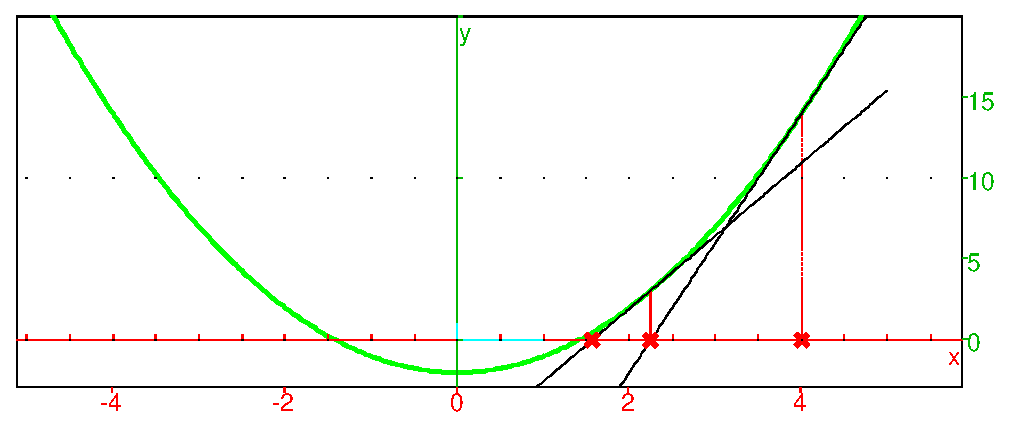
\includegraphics[width=\textwidth]{newsq}\\
On remarquera que :
{\tt plotnewton(sq-2,4,2)[0]}
renvoie :\\
{\tt 113/72 $\simeq$ 1.56944444444}\\
On tape :
{\tt plotnewton(ln-1,5,2)}\\
pour obtenir les termes $x_0,x_1,x_2$ de la suite de Newton qui converge 
vers $e$ et o\`u $x_0=5$ :\\
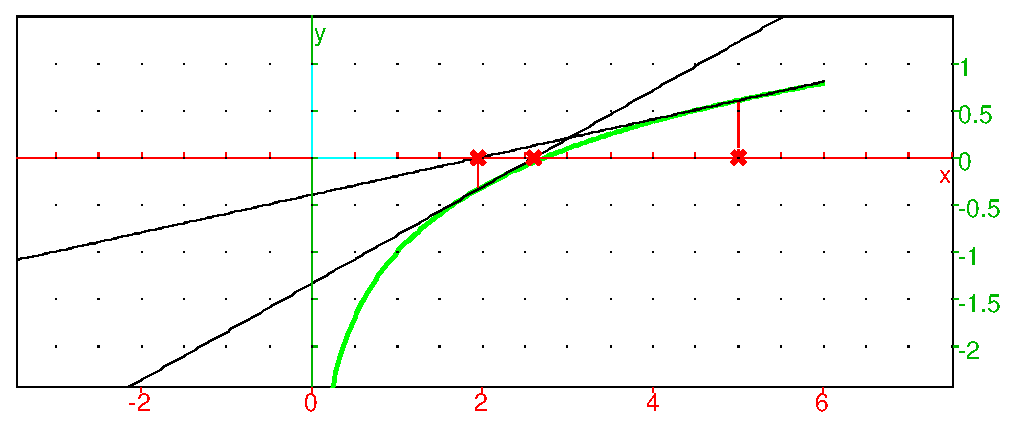
\includegraphics[width=\textwidth]{newlog}\\
On peut aussi faire une animation, pour cela, on tape :  
\begin{verbatim}
newtonsuite(f,a,p):={
local L,P,m,j,b,LT;
P:=point(a,couleur=point_width_4+rouge);
LT:=P;
f1:=function_diff(f);
for (j:=1;j<=p;j++) {
b:=f(a);
L:=L,segment(a,a+i*b,couleur=ligne_tiret+rouge);
m:=f1(a);
L:=L,plotfunc(b+(x-a)*m,x);
if (m==0){return "pente nulle"}
a:=a-f(a)/m;
P:=point(a,couleur=point_width_4+rouge);
LT:=LT,[LT,L,P];
}
print(affixe(P));
return LT;
};
animnewton(f,a,p):={
local LT;
LT:=newtonsuite(f,a,p);
return plotfunc(f(x),x,affichage=vert),animation(LT);
};
\end{verbatim}
On tape :
{\tt animnewton(sq-2,4,3)}\\

Puis, on \'ecrit la fonction {\tt newton\_rac} qui renvoie la valeur 
approch\'ee \`a $eps$ pr\`es de la racine de 
$f(x)=0$ on commen\c{c}ant l'it\'eration avec $x0$.\\
On remarquera que le param\`etre $f$ est une fonction et donc, que sa 
d\'eriv\'ee est la fonction {\tt g:=function\_diff(f)}.\\
On cherche une valeur approch\'ee donc il faut \'ecrire :\\
{\tt x0:=evalf(x0-f(x0)/g(x0))}\\
car si on ne met pas {\tt evalf},  les calculs  de l'it\'eration se feront
  excactement et seront vite compliqu\'es.
\begin{verbatim}
newton_rac(f,x0,eps):={
local x1,h,g;
g:=function\_diff(f)
x0:=evalf(x0-f(x0)/g(x0));
x1:=x0-f(x0)/g(x0);
if (x1>x0) {h:=eps;} else {h:=-eps;}
while (f(x1)*f(x1+h)>0){
   x1:=x1-f(x1)/g(x1);
}
return x1;
}
\end{verbatim}

\subsection{Exercices sur la m\'ethode de Newton}
\begin{enumerate}
\item
{\bf L'\'enonc\'e}
\begin{enumerate}
\item \'Etudier rapidement les variations de $f(x)=x\exp(x)+0.2$ pour montrer que l'\'equation $f(x)=0$ a deux solutions $a$ et $b$ qui v\'erifient $a<-1<b<0$
\item Calculer \`a l'aide d'un programme par la m\'ethode de Newton, 
les valeurs approch\'ees de $a$ et de $b$ obtenues apr\`es 5 it\'erations.
\item Modifier votre programme pour avoir des valeurs de $a$ et $b$ avec une 
pr\'ecision de  $eps$ (par exemple de $1e-6$).
\item \'Ecrire un programme qui dessine le graphe de la fonction implicite
$x\exp(x)+y\exp(y)=0$ lorsque $x\geq-5$.
\end{enumerate}

{\bf La solution avec {\tt Xcas}}
\begin{enumerate}
\item Pour avoir les variations de $f(x)=x\exp(x)+0.2$ on peut calculer la 
d\'eriv\'ee et faire le graphe de $f$.\\
On tape :
{\tt f(x):=x*exp(x)+0.2}\\
{\tt factor(diff(f(x)))}\\
On obtient : {\tt (x+1)*exp(x)}\\
On tape :
{\tt G:=plotfunc(f(x),x=-3..1)}\\
On obtient :\\

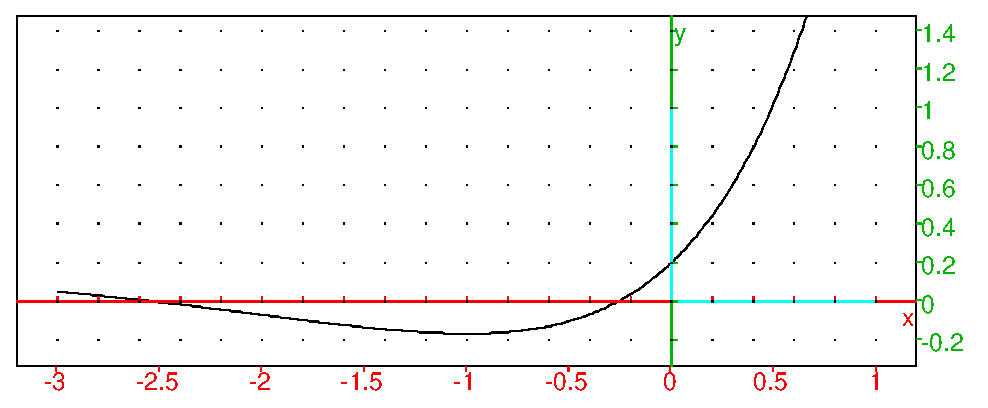
\includegraphics[width=\textwidth]{xex02}

Pour montrer que l'\'equation $f(x)=0$ a deux solutions $a$ et $b$ qui 
v\'erifient $a<-1<b<0$, on calcule, d'apr\`es le graphe 
$f(-3),f(-2),f(-1),f(0)$.\\
On tape :
{\tt f(x)\$(x=-3..0)}\\
On obtient : \\
{\tt 0.0506387948964,-0.0706705664732,-0.167879441171,0.2}\\
donc puisque $f$ est continue, d'apr\`es le th\'eor\`eme des valeurs interm\'ediaires on a : $-3<a<-2$ et $-1<b<0$\\
\item La m\'ethode de Newton consiste \`a it\'erer la fonction
$h$ d\'efinie par $h(x)=x-f(x)/g(x)$ o\`u $g$ est la deriv\'ee de $f$.
Pour trouver $a$, on va commencer en $x_0=-2$ (car la fonction est concave et 
d\'ecroissante sur $[-3;-2]$ et les $x_n$ seront des valeurs approch\'ees de 
$a$ par exc\'es)
et pour trouver $b$, on va commencer en $x_0=0$ (car la fonction est convexe et
croissante sur $[-1;0]$ et les $x_n$ seront des valeurs approch\'ees de $b$ par
exc\'es). 
On tape :
\begin{verbatim}
Newtonvaleur(x0):={
  local j,f,g,h;
  f(x):=x*exp(x)+0.2;
  g(x):=(x+1)*exp(x);
  h(x):=x-f(x)/g(x);
  pour j de 1 jusque 5 faire
    x0:=h(x0);
  fpour;
  retourne x0;
}:;
\end{verbatim}
{\bf Remarque} \\
On peut remplacer {\tt g(x):=(x+1)*exp(x);} par {\tt g:=function\_diff(f);}\\
On tape pour avoir la valeur de $x_5$ qui approche $a$ :\\ 
{\tt Newtonvaleur(-2.)}\\
On obtient : \\
{\tt -2.54264135777}\\
On tape pour avoir la valeur de $x_5$ qui approche $b$  :\\ 
{\tt Newtonvaleur(0)}\\
On obtient : \\
{\tt -0.259171101819}

\item Si on veut avoir une valeur approch\'ee de $a$ (resp $b$) \`a $eps$ 
pr\'es, il faut avoir un $x_j$ qui v\'erifie $x_j-eps\leq a<x_j$ 
(resp $x_j-eps \leq b<x_j$) c'est \`a dire  $f(x_j-eps)>0$ (resp 
$f(x_j-eps)<0$) i.e. on doit avoir dans les 2 cas, $f(x_j-eps)*f(x0)\leq 0$.\\ 
On tape :
\begin{verbatim}
Newtonvalpres(x0,eps):={
  local j,g,h,t,s;
  f(x):=x*exp(x)+0.2;
  g(x):=(x+1)*exp(x);
  h(x):=x-f(x)/g(x);
  j:=0;
  t:=x0-eps;
  //s:=ifte(f(x0)>0,1,-1);
  s:=sign(f(x0));
  tantque s*f(t)>0 faire
    x0:=h(x0);
    t:=x0-eps;
    j:=j+1;
  ftantque;
  print(j);
  retourne t,x0;
}:;
\end{verbatim}
On tape pour avoir la valeur de $x_j$ qui donne un encadrement de $a$ \`a 
$1e-6$ pr\'es :\\ 
{\tt Newtonvalpres(-2.,1e-6)}\\
On obtient pour $j=3$ : \\
{\tt -2.54264235686,-2.54264135686}\\
On tape pour avoir la valeur de $x_j$ qui donne un encadrement de $a$ \`a 
$1e-10$ pr\'es :\\ 
{\tt Newtonvalpres(-2.,1e-10)}\\
On obtient  pour $j=4$ : \\
{\tt -2.54264135787,-2.54264135777}\\
On tape pour avoir la valeur de $x_j$ qui donne un encadrement de $b$ \`a 
$1e-6$ pr\'es :\\ 
{\tt Newtonvalpres(0,1e-6)}\\
On obtient  pour $j=4$ : \\
{\tt -0.259172101477,-0.259171101477}
On tape pour avoir la valeur de $x_j$ qui donne un encadrement de $b$ \`a 
$1e-10$ pr\'es :\\ 
{\tt Newtonvalpres(0,1e-10)}\\
On obtient  pour $j=5$ : \\
{\tt -0.259171101919,-0.259171101819}

\item $y\exp(y)+a=0$ a une solution si $-\exp(-1)+a \leq 0$ i.e si $a<1/e$
Cette fonction est d\'efinie pour des $x$ tels que $x\exp(x)=a<1/e$. 
On r\'esout donc l'\'equation $x\exp(x)-1/e=0$:\\
On modifie le programme en :\\
\begin{verbatim}
Newtonvaleura(x0,a):={
  local j,f,g,h;
  f(x,a):=x*exp(x)+a;
  g(x):=(x+1)*exp(x);
  h(x):=x-f(x,a)/g(x);
  pour j de 1 jusque 5 faire
    x0:=h(x0);
  fpour;
  retourne x0;
}:;
\end{verbatim}
lorsque $a=-1/e$, on a $f(0,a)=a<0$ et $f(1,a)=e-1/e>0$.
On tape :\\
{\tt Newtonvaleura(1,-1./e)}\\
On obtient :\\
{\tt  0.278464542823}\\
Pour $x\leq 0$, $a=x*\exp(x)\leq 0$  donc l'\'equation en $y$, 
$y*\exp(y)+x*\exp(x)=0$ a une seule solution positive
($y*\exp(y)+a$ vaut $a\leq 0$ pour $y=0$  et vaut $(x(exp(x)^2-1)/(exp(x))>0$ 
pour $y=-x$). On peut donc l'obtenir par la m\'ethode de Newton : on d\'emarre 
avec $y_0=-a$ car pour $x>0$ la courbe de $f(x,a)=x*\exp(x)+a$ se trouve au 
dessus de sa tangente en $x=0$ (puisque $f"(x)>0$ pour $x>0$) et que cette 
tangente d'\'equation $y=x+a$ coupe l'axe des $x$ en $x=-a$.\\
Pour $0<x<0.278464542823$ l'\'equation en $y$, $y*\exp(y)+x*\exp(x)=0$ a deux 
solutions que l'on peut obtenir par la m\'ethode de Newton : on d\'emarre soit 
par $x_0=0$ soit par $x_0=-2$.\\
On tape (on choisit de prendre $x_5$ comme valeur approch\'ee) :
\begin{verbatim}
Newtonimplicit():={
  local j,f,g,h,a,xj,y0,y,L;
  g(y):=(y+1)*exp(y);
  f(y,a):=y*exp(y)+a;
  pour xj de -4 jusque 0 pas 0.1 faire
  a:=xj*exp(xj);
  h(y):=y-f(y,a)/g(y);
  y0:=-a;
  pour j de 1 jusque 5 faire
    y0:=h(y0);
  fpour;
  L:=L,point(xj+i*y0);
fpour;
L:=L,point(0.28-i);
pour xj de 0.01 jusque 0.28 pas 0.02 faire
  a:=xj*exp(xj);
  h(y):=y-f(y,a)/g(y);
  y0:=0;
  pour j de 1 jusque 5 faire
    y0:=h(y0);
  fpour;
  L:=L,point(xj+i*y0);
  y0:=-2;
  pour j de 1 jusque 5 faire
    y0:=h(y0);
  fpour;
  L:=L,point(xj+i*y0)
fpour;
retourne L;
}:;
\end{verbatim}
On tape {\tt Newtonimplicit()}\\
On obtient :\\

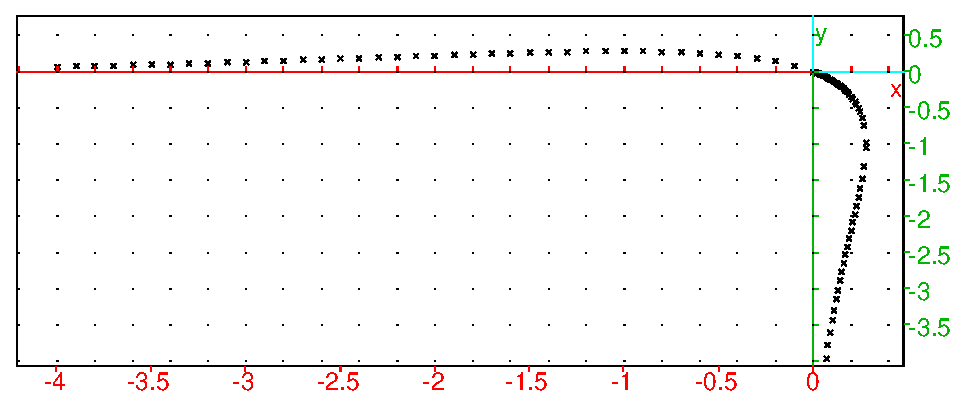
\includegraphics[width=\textwidth]{xexyey}

On peut aussi vouloir calculer $y$ \`a $eps$ -pr\`es. Mais attention lorsqu'on 
part de $y0=-2$ on obtient une valeur soit par d\'efaut, soit par exc\'es selon
le signe de $f(-2,a)$ (si $f(-2,a)>0$ ce sera par exc\`es car pour $x=-2$ on a 
un point d'inflexion).\\
On tape alors :
\begin{verbatim}
Newtonimpl(eps):={
  local j,f,g,h,a,xj,y0,y,t,s,L;
  g(y):=(y+1)*exp(y);
  f(y,a):=y*exp(y)+a;
  L:=NULL;
  pour xj de -5 jusque 0 pas 0.05 faire
  a:=evalf(xj*exp(xj));
  h(y):=y-f(y,a)/g(y);
  y0:=-a;
  t:=y0-eps;
  s:=sign(f(y0,a));
  tantque s*f(t,a)>0 faire
    y0:=h(y0);
    t:=y0-eps;
  ftantque;
  L:=L,point(xj+i*y0);
fpour;
L:=L,point(0.28-i);
pour xj de 0.01 jusque 0.28 pas 0.02 faire
  a:=evalf(xj*exp(xj));
  h(y):=y-f(y,a)/g(y);
  y0:=0.;
  t:=y0-eps;
  s:=sign(f(y0,a));
  tantque s*f(t,a)>0 faire
    y0:=h(y0);
    t:=y0-eps;
  ftantque;
  L:=L,point(xj+i*y0);
fpour;
  pour xj de 0.01 jusque 0.28 pas 0.02 faire
    a:=evalf(xj*exp(xj));
  h(y):=y-f(y,a)/g(y);
  y0:=-2.;
  s:=sign(f(y0,a));
  si s>0  alors eps:=-abs(eps); fsi; 
  t:=y0-eps;
  tantque s*f(t,a)>0 faire
    y0:=h(y0);
    t:=y0-eps;
  ftantque;
  L:=L,point(xj+i*y0)
fpour;
retourne L;
}:;
\end{verbatim}
On tape {\tt Newtonimpl(0.01)}\\

On peut v\'erifier en tapant :\\
{\tt plotimplicit(x*exp(x)+y*exp(y),[x,y])}
\end{enumerate}

\item
{\bf L'\'enonc\'e}\\
Donner la valeur approch\'ee de $\cos(x)=x$ pour $x\in [0;1]$ obtenue en 
partant de $x_0=0$ apr\`es 4, puis apr\`es 10 it\'erations lorsque :
\begin{enumerate}
\item On applique la m\'ethode du point fixe \`a $f(x)=\cos(x)$.
\item On applique la m\'ethode de Newton.
\item On applique la m\'ethode du $\Delta^2$ d'Aitken.
\item On applique la m\'ethode de Steffensen.
\end{enumerate}
Quelle m\'ethode vous semble la meilleure ? Expliquez pourquoi.

{\bf La solution avec {\tt Xcas}}\\
On configure {\tt Xcas} avec 20 digits.
\begin{enumerate}
\item fa fonction $f(x)=\cos(x)$ est $\sin(1)$-contractante sur [0;1], car 
d'apr\`es le th\'eor\`eme des accroissements finis :\\ 
il existe $c\in [0;1]$ tel que pour tout $x_1\in [0;1]$ et tout $x_2\in [0;1]$
on a $\cos(x_1)-\cos(x_2)=(x_1-x_2)\sin(c)$ donc\\
$|\cos(x_1)-\cos(x_2)|=|x_1-x_2||\sin(c)|\leq |x_1-x_2|\sin(1)$.\\
On tape :
\begin{verbatim}
ptfixecos(x0,n):={
local j,f;
f(x):=cos(x);
pour j de 1 jusque n faire
  x0:=f(evalf(x0));
fpour;
retourne x0;
}:;
\end{verbatim}
On tape : {\tt ptfixecos(0,4)}\\
On obtient : {\tt 0.654289790497779149974}\\
On tape : {\tt ptfixecos(0,10)}\\
On obtient : {\tt 0.731404042422509858293}\\
\item On pose $F(x)=\cos(x)-x$ et on a $F'(x)=-\sin(x)-1$, on va donc it\'erer
la fonction $g(x)=x-F(x)/F'(x)=(x*\sin(x)+\cos(x))/(\sin(x)+1)$.\\
On tape :
\begin{verbatim}
Newtoncos(x0,n):={
local j,g,F,dF;
F(x):=cos(x)-x;
dF:=function_diff(F);
//g(x):=(x*sin(x)+cos(x))/(sin(x)+1);
g(x):=normal(x-F(x)/dF(x));
pour j de 1 jusque n faire
  x0:=g(evalf(x0));
fpour;
retourne x0;
}:;
\end{verbatim}
On tape : {\tt Newtoncos(0,4)}\\
On obtient : {\tt 0.739085133385283969762}\\
On tape : {\tt Newtoncos(0,10)}\\
On obtient : {\tt 0.739085133215160641651}\\
\item La m\'ethode du $\Delta^2$ d'Aitken consiste \`a transformer la suite des
it\'er\'ees du point fixe par la fonction :\\
$gs(x)=x-(f(x)-x)*(f(x)-x)/(f(f(x))-2f(x)+x)$ avec $f(x)=\cos(x)$.\\
On tape :
\begin{verbatim}
Aitkencos(x0,n):={
local j,gs,f,y0;
f(x):=cos(x);
gs(x):=x-(f(x)-x)*(f(x)-x)/(f(f(x))-2f(x)+x);
pour j de 1 jusque n faire
  x0:=f(evalf(x0));
  y0:=gs(x0);
fpour;
print(x0);
retourne y0;
}:;
\end{verbatim}
On tape : {\tt Aitkencos(0,4)}\\
On obtient : {\tt 0.738050421371663847259}\\
On tape : {\tt Aitkencos(0,10)}\\
On obtient : {\tt 0.739076383318955862683}\\
\item La m\'ethode de Steffenson consiste \`a it\'erer la fonction :\\
$gs(x)=x-(f(x)-x)*(f(x)-x)/(f(f(x))-2f(x)+x)$ avec $f(x)=\cos(x)$.\\
On tape :
\begin{verbatim}
Steffensencos(x0,n):={
local j,gs,f;
f(x):=cos(x);
gs(x):=x-(f(x)-x)*(f(x)-x)/(f(f(x))-2f(x)+x);
pour j de 1 jusque n faire
  x0:=gs(evalf(x0));
fpour;
retourne x0;
}:;
\end{verbatim}
On tape : {\tt Steffensencos(0,4)}\\
On obtient : {\tt 0.739085133215160534355}\\
On tape : {\tt Steffensencos(0,10)}\\
On obtient : {\tt 0.739085133215160641651}\\
\end{enumerate}
Les m\'ethodes de Newton et de Steffensen sont plus performantes car ce sont 
des m\'ethodes d'ordre 2 (la fonction que l'on i\'ere a une d\'eriv\'ee nulle 
au point solution de $f(x)=\cos(x)=x$).\\
M\^eme avec  {\tt Digits:=30} on a :\\
{\tt Steffensencos(0,6)=Steffensencos(0,10)=\\
 Newtoncos(0,6)=Newtoncos(0,10)=\\
0.7390851332151606416553120876735}

\item {\bf L'\'enonc\'e}\\
Dans un probl\`eme de baccalaur\'eat, on se propose de calculer des valeurs approch\'ees des solutions de $\exp(-x)\cos(x)=x$ sur $[-\pi/2;\pi/2]$.
\begin{enumerate}
\item D\'eterminer le nombre de solutions.
\item Donner un algorithme de calcul et \'ecrire le programme correspondant.
\item Donner un encadrement de la solution ?
\item Dessiner les points de coordonn\`ees $t,x$ qui v\'erifient :\\
$\exp(-x)\cos(x)-x+t=0$ pour  $t \in [-\pi/2;\pi/2]$ et  $x \in [-\pi/2;\pi/2]$
\end{enumerate}
{\bf La solution avec {\tt Xcas}}\\
\begin{enumerate}
\item On tape : {\tt f(x:)=exp(-x)*cos(x)-x}\\
 {\tt f1:=function\_diff(f);f2:=normal(diff(f1(x)))}
On trouve :\\
{\tt f1(x)=(-cos(x)-sin(x))*exp(-x)-1} et \\
{\tt f2=2*exp(-x)*sin(x)}\\
 On a :\\
$f2=0$ en $x=0$ le point(0,1) est donc un point d'inflexion et \\
sur $[-\pi/2;0]$, on a $f2<0$  et sur $[0;\pi/2]$, on a  $f2>0$\\
On a :\\
$f1(x)=\exp(\pi/2)-1>0$ pour $x=-\pi/2$\\
$f1(0)=-2$ \\
$f1(x)=-\exp(-\pi/2)-1 <0$ pour $x=\pi/2$\\
$f1$ s'annule donc pour $x=a<0$ et donc $f$ est croissante puis d\'ecroissante
et comme on a $f(-pi/2)=pi/2$, $f(0)=1$ et $f(pi/2)=-pi/2$ et $f$ continue,
$f$ s'annule en un seul point $x=b>0$
 Pour v\'erifier, on tape : \\
{\tt G:=plotfunc(f(x),x=-pi/2..pi/2);tangente(G,0)}\\
\item On peut appliquer la m\'ethode de Newton en partant de $x_0=0.0$, la 
suite $x_n=x_{n-1}-f(x_{n-1})/f1(x_{n-1})$ va donner une valeur approch\'ee par 
d\'efaut de $b$ car sur $[0;b]$ $f$ est positive d\'ecroissante et convexe.

On tape :\\
{\tt Newton0(4)}\\
On obtient avec 22 digits:\\
{\tt 0.51775736368245829829471}\\
\item 
On tape  :
\begin{verbatim}
Newton0(n):={
local j,f,f1,g,x0;
f(x):=exp(-x)*cos(x)-x;
f1:=function_diff(f);
g(x):=normal(x-f(x)/f1(x));
x0:=0.0;
pour j de 1 jusque n faire
x0:=g(x0)
fpour;
retourne x0;
}:;
\end{verbatim}
\item
Pour avoir un encadrement de la solution \`a {\tt eps} pr\`es, on continue 
l'it\'eration tant que la valeur de $f(x_n+eps)$ reste strictement positive.\\
On tape
\begin{verbatim}
Newtoneps(n,eps):={
  local j,f,f1,g,x0;
  f(x):=exp(-x)*cos(x)-x;
  f1:=function_diff(f);
  g(x):=normal(x-f(x)/f1(x));
  x0:=0.0;
  j:=0;
  tantque f(x0+eps)>0 faire
    x0:=g(x0);
    j:=j+1;
  ftantque;
  print(j);
  retourne x0,x0+eps;
}
:;
\end{verbatim}
On tape :\\
{\tt Newtoneps(0,1e-20)}\\
On obtient :\\
{\tt 0.51775736368245829832277,0.51775736368245829833277}\\
\item Il faut voir que si on remplace $f(x)$ par $f(x)+t$ la suite d\'efinie 
par :$x_0=0$ et $x_{n+}=x_n-(f(x_n)+t)/f1(x_n)$ 
 approche la solution en $x$ de $f(x)+t=0$ par exc\`es si $t<-1$ et par 
d\'efaut si $t>-1$ car pour $x=0$ la fonction $f(x)+t$ a un point d'inflexion
qui est le point $(0;1+t)$.
De plus $f(x)+t>1+t$ pour $x<0$ et $f(x)+t<1+t$ pour $x>0$. Donc si
$1+t>0$ la solution sera positive et si $1+t<0$ la solution sera negative \\
On tape :
\begin{verbatim}
Newtonimpl():={
  local j,f,f1,g,x0,t,a,L;
  a:=evalf(pi/2);
  f(x):=exp(-x)*cos(x)-x;
  f1:=function_diff(f);
  L:=NULL;
    pour t de -a jusque -1 pas 0.1 faire
      g(x):=normal(x-(f(x)+t)/f1(x));
      x0:=0.0;
      tantque f(x0-0.01)+t<0 faire
        x0:=g(x0);
      ftantque;
      L:=L,point(t,x0);
    fpour;
    pour t de -1 jusque a pas 0.1 faire
      g(x):=normal(x-(f(x)+t)/f1(x));
      x0:=0.0;
      tantque f(x0+0.01)+t>0 faire
        x0:=g(x0);
      ftantque;
      L:=L,point(t,x0);
    fpour;
    return L;
  }
:;
\end{verbatim}
On tape :\\
{\tt Newtonimpl()}\\
On obtient :\\

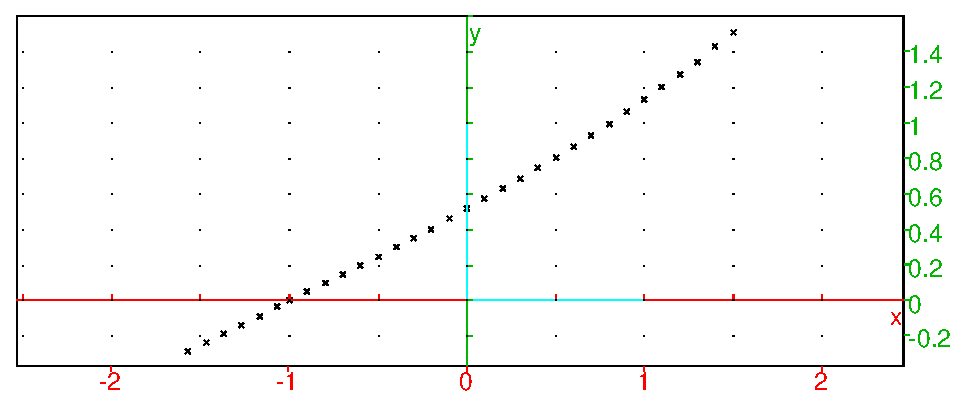
\includegraphics[width=\textwidth]{Newtonimpl}
\end{enumerate}


\end{enumerate}

\subsection{La m\'ethode de Newton avec pr\'efacteur}
Lorsqu'on part d'une valeur $x_0$ trop \'eloign\'ee de la racine de $f(x)$
(si par exemple $|f(x_0)|$ est grand),
on a int\'er\^et \`a utiliser un pr\'efacteur pour se rapprocher plus vite de 
la solution de $f(x)=0$.\\
Posons $\displaystyle n(x)=-\frac{f(x)}{f'(x)}$, on a alors :
$$\lim_{h \rightarrow 0}\frac{(f(x_0+h*n(x_0))-f(x_0))}{h*n(x_0)}=f'(x_0)$$
donc 
$$\lim_{h \rightarrow 0}\frac{(f(x_0+h*n(x_0))-f(x_0))}{h}=n(x_0)*f'(x_0)=-f(x_0)$$
ce qui veut dire que :\\
$f(x_0+h*n(x_0))=f(x_0)(1-h)+h\cdot \epsilon(h)$ avec $\epsilon(h)$ tend vers 0
 quand $h$ tend vers 0.\\
Donc, il existe $h_0$ v\'erifiant :\\
$|f(x_0+h_0*n(x_0))|<|f(x_0)|$\\
Remarque : Il faut minimiser $|f(x_0+h_0*n(x_0))|$. 
or plus $h_0$ est proche de 1 et plus $|f(x_0)*(1-h_0)|$ sera petit. 
Par exemple, on prendra le plus grand $h_0$, dans la liste 
$[1,3/4,(3/4)^2,...]$ qui v\'erifie $|f(x_0+h_0*n(x_0))|<|f(x_0)|$\\
Pour cette valeur de $h_0$, $x_0+h_0*n(x_0)$ est probablement plus 
proche de la racine que $x_0$ : on dit que $h_0$ est le pr\'efacteur de la 
m\'ethode de Newton.\\
On va choisir par exemple au d\'ebut $h_0=1$, et on regarde si 
$|f(x_0+n(x_0))|<|f(x_0)|$,
si ce n'est pas le cas on prend $h_0=(3/4)$ et on regarde si 
$|f(x_0+3/4*n(x_0))|<|f(x_0)|$,
si ce n'est pas le cas on prend $h_0=(3/4)^2$ etc...\\ 
On change de pr\'efacteurs \`a chaque \'etape jusqu'\`a ce que :
$abs(f(x1))-abs(f(x0))<0$ sans pr\'efacteur,
on continue alors l'it\'eration sans pr\'efacteur, c'est \`a dire avec la 
m\'ethode de Newton normale. 
On \'ecrit donc :
\begin{verbatim}
newton_prefacts(f,x0,eps):={
local x1,h,h0,prefact,niter;
//prefact est egal par ex a 3/4
h0:=1.0;
niter:=0;
prefact:=0.75;
x1:=x0-h0*f(x0)/function_diff(f)(x0);
while (abs(f(x1))-abs(f(x0))>0) {
   h0:=h0*prefact;
   x1:=x0-h0*f(x0)/function_diff(f)(x0);
} 
h:=eps;
while (h0!=1 and niter<100){
   x0:=x1;
   x1:=x1-h0*f(x1)/function_diff(f)(x1);
   while (abs(f(x1))-abs(f(x0))>0) {
      h0:=h0*prefact;
      x1:=x0-h0*f(x0)/function_diff(f)(x0);
   } 
   while (abs(f(x1))-abs(f(x0)<0 and h0!=1)) {
      h0:=h0/prefact;
      x1:=x0-h0*f(x0)/function_diff(f)(x0);
   } 
niter:=niter+1;   
}
while (f(x1-h)*f(x1+h)>0  and niter<200){
   x0:=x1;
   x1:=x1-f(x1)/function_diff(f)(x1);
   niter:=niter+1;
}

if  (niter<200) {return x1;} else {return "pas trouve";} 
}
\end{verbatim}
On d\'efinit la fonction $f$ par  ${\tt f(x):=x^2-2}$ et on met ce programme 
dans un niveau \'editeur de programmes (que l'on ouvre avec {\tt Alt+p}), puis 
on le teste et on le valide avec {\tt OK}.\\
 On tape :\\
{\tt newton\_prefacts(f,100,1e-10)}\\
On obtient :\\
{\tt 1.41421356237}
On tape :\\
{\tt newton\_prefacts(f,3,1e-5)}\\
On obtient :\\
{\tt 1.41421378005}

\section{Trouver un encadrement de $x0$ lorsque $f(x0)$ est minimum}
Soit $f$ une fonction d\'efinie sur $[a;b]$. On suppose que $f$ est unimodale 
sur $[a;b]$, c'est \`a dite que $f$ a un seul extremum sur $[a;b]$. On suppose 
de plus que cet extremum est un minimum (sinon on remplacera $f$ par $-f$.)
On se propose de trouver un encadrement \`a $eps$ pr\`es de la valeur pour 
laquelle $f$ est minimum.
\subsection{D\'escription du principe de la m\'ethode}
On partage $[a;b]$ en trois morceaux en consid\'erant $c$ et $d$ 
v\'erifiant : $a<c<d<b$.\\ 
On calcule $f(c)$ et $f(d)$ et on les compare.\\
Puisque $f$ a un seul minimum sur $[a;b]$ elle d\'ecroit, passe par son 
minimum, puis $f$ croit. Selon les trois cas possibles on a :
\begin{itemize}
\item f(c)<f(d)\\
dans ce cas, la valeur pour laquelle $f$ est minimum n'appartient pas \`a 
$[d;b]$
\item f(c)>f(d)\\
dans ce cas, la valeur pour laquelle $f$ est minimum n'appartient pas \`a  
$[a;c]$
\item f(c)=f(d)\\
dans ce cas, la valeur pour laquelle $f$ est minimum n'appartient pas \`a 
$[d;b]$ ni \`a $[a;c]$
\end{itemize}
Ainsi, l'intervalle de recherche a diminu\'e et on peut recommencer le 
processus. Pour que l'algorithme soit performant,
on veut que l'intervalle de recherche diminue rapidement et que le nombre de 
valeurs de $f$ \`a calculer soit le plus petit possible. Pour cela comment 
doit-on choisir $c$ et $d$ ?  
\subsection{D\'escription de 2 m\'ethodes}
\subsubsection{On fait presque une dichotomie}
On choisit $c$ et $d$ proche de $\frac{a+b}{2}$ par exemple :\\
 $c=\frac{a+b-eps}{2}$ et $d=\frac{a+b+eps}{2}$ pour $eps$ donn\'e.
Dans ce cas, \`a chaque \'etape l'intervalle diminue presque de moiti\'e mais 
on doit calculer, \`a chaque \'etape, deux valeurs de $f$. 
\subsubsection{On utilise la suite de Fibonacci}
Comment faire pour que l'une des valeurs de $f$ d\'ej\`a calcul\'ee serve 
\`a l'\'etape suivante ?\\
La solution se trouve dans la suite de Fibonacci, suite d\'efinie par :\\
$u_0=1$, $u_1=2$, $u_n=u_{n-2}+u_{n-1}$ dont les premiers termes sont :
$1,2,3,5,8,13,21,34,55,89...$
Par exemple si on partage $[a;b]$ en 89 parties \'egales si $l=(b-a)/89$,
on choisit $c=a+34*l$ et $d=a+55*l$ et ainsi on a :\\
$c-a=34*l$, $d-c=21*l$, $b-d=34*l$ (car 89=55+34 et 34+21=55 puisque 
21,34,55,89 sont des termes cons\'ecutifs de  la suite de Fibonacci).\\
On calcule $f(c)$ et $f(d)$ puis on r\'eduit l'intervalle en un intervalle de
longueur $(b-a)*55/89$, par exemple si l'intervalle suivant est $[a;d]$ et, si 
on recommence le processus, le point $c$ est le futur point $d$.\\
Donc \`a chaque \'etape il suffit de calculer une seule valeur de $f$ pour
passer de l'intervalle $[a;b]$ (proportionnel \`a $u_n$) \`a l'intervalle 
$[a;d]$ ou $[c;b]$ (proportionnel \`a $u_{n-1}$). Il y a bien s\^ur le cas 
$f(c)=f(d)$ o\`u il faut \`a l'\'etape suivante calculer deux valeurs de $f$, 
mais dans ce cas on gagne 3 \'etapes car on passe de l'intervalle $[a;b]$ 
(proportionnel \`a $u_n$) \`a l'intervalle $[c;d]$ (proportionnel \`a 
$u_{n-3}$).\\
Selon la valeur $eps$ de la longueur de l'encadrement, on calcule
$k:=ceil(2*(b-a)/eps);$ et la premi\`ere valeur $t=u_n$ de la suite de 
Fibonacci sup\'erieure \`a $k$. il faut alors diviser l'intervalle $[a;b]$ en 
$t$ parties \'egales. On applique alors plusieurs fois le processus et on 
s'arr\^ete quand $n=1$, c'est \`a dire quand l'intervalle a \'et\'e r\'eduit 
\`a un intervalle de longueur $2*(b-a)/t$ qui est, grace au choix de $t$ 
($t>k>2*(b-a)/eps$) inf\'erieur \`a $eps$.
\subsection{Traduction {\tt Xcas} de l'algorithme avec Fibonacci}
\begin{verbatim}
//f(x):=2*x^4-10*x^3-4*x^2+100
//fibomin(f,1,5,0.000001)
//g(x):=2*x^4-10*x^3+4*x^2+100
//fibomin(g,1,5,1e-20)
//calcul la valeur du min d'une fonction ayant 
//un seul extrema sur [a,b]
fibomin(f,a,b,eps):={
  local c,d,F,k,n,t,g,h,l,fc,fd;
  if (a>b) {c:=a;a:=b;b:=c;}
  k:=ceil(2*(b-a)/eps);
  F:=1,2;
  n:=1;
  g:=1;
  t:=2;
  //construction de F=la suite de Fibonacci
  //h,g,t sont 3 termes consecutifs de F
  while (t<k) {
    n:=n+1;
    h:=g;
    g:=t;
    t:=h+g;
    F:=F,t;
  }
  l:=(b-a)/t;
  c:=a+h*l;
  d:=a+g*l;
  fc:=f(c);
  fd:=f(d);
  //on itere le processus et on s'arrete qd n=1
  while (n>1) {
    if (fc>fd) {
      a:=a+h*l;
      fc:=fd;
      t:=h;
      h:=g-h;
      g:=t;
      fd:=f(a+g*l);
      n:=n-1;
    }else{
      if (fc<fd) {
	b:=a+g*l;
	t:=h;
	h:=g-h;
	g:=t;
	fd:=fc;
	fc:=f(a+h*l);
	n:=n-1;
      }else{
	a:=a+h*l;
	b:=b-h*l;
	t:=g-h;
	g:=h-t;
	h:=t-g;
	fc:=f(a+h*l);
	fd:=f(a+g*l);
	n:=n-3;
      }
    }
  }
  return [a,b];
}
\end{verbatim}
On tape :\\
{\tt f(x):=x\verb|^|4-10}\\
{\tt fibomin(f,-1,1,1e-10)}\\
On obtient :\\
{\tt [(-1)/53316291173,1/53316291173]}\\
On tape :\\
{\tt g(x):=2*x\verb|^|4-10*x\verb|^|3-4*x\verb|^|2+100}\\
{\tt fibomin(g,1,5,1e-10)}\\
On obtient :\\
{\tt [86267571271/21566892818,86267571273/21566892818]}
On tape :\\
{\tt h(x):=2*x\verb|^|4-10*x\verb|^|3+4*x\verb|^|2+100}\\
{\tt fibomin(h,1,5,1e-10)}\\
On obtient :\\
{\tt [74644573011/21566892818,74644573013/21566892818]}\\

\chapter{Algorithmes d'alg\'ebre}
\section{M\'ethode pour r\'esoudre des syst\`emes lin\'eaires}
%On appelle matrice principale d'une matrice rectangulaire $M$ (de dimension $n \times p$) une matrice carr\'ee contenue dans $M$ de dimension $min(n,p)$.
Dans {\tt Xcas}, il existe d\'ej\`a les fonctions qui correspondent
aux  algorithmes qui suivent, ce sont :
{\tt ref, rref, ker, pivot} 
\subsection{Le pivot de Gauss quand $A$ est de rang maximum}
 \'Etant donn\'e un syst\`eme d'\'equations not\'e $AX=b$, on cherche \`a le 
remplacer par un syst\`eme \'equivalent et triangulaire inf\'erieur.\\
\`A un syst\`eme d'\'equations $AX=b$, on associe la  matrice $M$ form\'ee 
par  $A$ que l'on  borde avec $b$ comme derni\`ere colonne.\\
La m\'ethode de Gauss (resp Gauss-Jordan) consiste \`a multiplier $A$ et $b$ 
(donc $M$) par des matrices inversibles, afin de rendre $A$ triangulaire 
inf\'erieure (resp diagonale). Cette transformation, qui  se fera au coup 
par coup en traitant toutes les colonnes de $A$ (donc toutes les colonnes de 
$M$, sauf la derni\`ere), consiste par des combinaisons de lignes de $M$ 
\`a mettre des z\'eros sous (resp de part et d'autre) la diagonale de $A$.\\  
La fonction {\tt gauss\_redi} ci-dessous, transforme $M$ par la m\'ethode de
 Gauss, la variable {\tt pivo} (car {\tt pivot} est une fonction de {\tt Xcas})
sert \`a mettre le pivot choisi.\\
 Pour $j=0..p-2$ ($p-2$ car on ne traite pas la derni\`ere colonne de $M$), 
dans chaque colonne $j$, on cherche ce qui va faire office de pivot \`a partir de la diagonale : dans le programme ci-dessous on choisit le premier 
\'el\'ement non nul, puis par un \'echange de lignes, on met le pivot sur la 
diagonale ($pivo=M[j,j]$). Il ne reste plus qu'\`a former, pour chaque ligne 
$k$ ($k>j$) et pour $a=M[k,j]$, la combinaison :\\
 $pivo*ligne_k-a*ligne_j$   (et ainsi $M[k,j]$ devient nul).\\
On \'ecrit pour r\'ealiser cette combinaison :\\
{\tt a:=M[k,j];\\
     for (l:=j;l<nc;l++)\{\\ 
          M[k,l]:=M[k,l]*pivo-M[j,l]*a;\}}\\
On remarquera qu'il suffit que  $l$ parte de $j$ car :\\
pour tout $l<j$, on a d\'ej\`a obtenu, par le traitement des colonnes 
$l=0..j-1$, $M[k,l]=0$.\\
Le programme ci-dessous ne sera utile que si on trouve un pivot pour 
chaque colonne : c'est \`a dire si la matrice $A$ est de rang maximum. 
En effet, dans ce programme, si on ne trouve pas de pivot (i. e. si tous les 
\'el\'ements d'une colonne sont nuls sur et sous la diagonale), on continue 
comme si  de rien \'etait...
\begin{verbatim}
gauss_redi(M):={
local pivo,j,k,nl,nc,temp,l,n,a;
nl:=nrows(M);
nc:=ncols(M);
n:=min(nl,nc-1);
//on met des 0 sous la diagonale du carre n*n
for (j:=0;j<n;j++) {
  //choix du pivot mis ds pivo
    k:=j;
    while (M[k,j]==0 and k<nl-1) {k:=k+1;}
    //on ne fait la suite que si on a pivo!=0
    if (M[k,j]!=0) {
      pivo:=M[k,j];
      //echange de la ligne j et de la ligne k
      for (l:=j;l<nc;l++){
       temp:=M[j,l];
       M[j,l] := M[k,l];
        M[k,l]:=temp;     
      }
     //fin du choix du pivot qui est M[j,j]
      for (k:=j+1;k<nl;k++) {
        a:=M[k,j];
        for (l:=j;l<nc;l++){ 
          M[k,l]:=M[k,l]*pivo-M[j,l]*a; 
         } 
       }
    }  
}
return M;
}
\end{verbatim} 
On tape :\\
{\tt M0:= [[1,2,3,6],[2,3,1,6],[3,2,1,6]]}\\
{\tt gauss\_redi(M0)}\\
On obtient :\\
{\tt [[1,2,3,6],[0,-1,-5,-6],[0,0,-12,-12]]}\\
On tape :\\
{\tt M1:= [[1,2,3,4],[0,0,1,2],[0,0,5,1]]}\\
{\tt gauss\_redi(M1)}\\
On obtient :\\
{\tt [[1,2,3,4],[0,0,1,2],[0,0,5,1]]}\\
On tape :\\
{\tt M2:= [[1,2,3,4],[0,0,1,2],[0,0,5,1],[0,0,3,2],[0,0,-1,1]]}\\
{\tt gauss\_redi(M2)}
On obtient :\\
{\tt [[1,2,3,4],[0,0,1,2],[0,0,5,1],[0,0,0,7],[0,0,0,6]]}\\
c'est \`a dire :
$${\tt gauss\_redi\left(\left [
\begin{array}{rrrr}
1&2&3&4\\
0&0&1&2\\
0&0&5&1\\
0&0&3&2\\
0&0&-1&1\\
\end{array}
\right ]\right )}=\left [
\begin{array}{rrrr}
1&2&3&4\\
0&0&1&2\\
0&0&5&1\\
0&0&0&7\\
0&0&0&0\\
\end{array}
\right ]
$$
\subsection{Le pivot de Gauss pour $A$ quelconque}
On cherche un  programme valable lorsque  $A$ est quelconque :
on veut, dans ce cas, mettre des z\'eros sous la "fausse diagonale" de $A$
(ce qu'on appelle "fausse diagonale" c'est la diagonale obtenue en ne tenant 
pas compte des colonnes pour lesquelles la recherche du pivot a \'et\'e 
infructueuse : un peu comme si ces colonnes \'etaient rejet\'ees \`a la fin 
de la matrice).\\
Donc, dans ce programme, si on ne trouve pas de pivot pour la colonne d'indice
$jc$ (i. e. si tous les \'el\'ements de la colonne $jc$ sont nuls sur et sous 
la diagonale), on continue en cherchant, pour la colonne suivante (celle 
d'indice $jc+1$), un pivot \`a partir de l'\'el\'ement situ\'e \`a la ligne 
d'indice $jc$ (et non comme pr\'ec\'edemment \`a partir de $jc+1$),
pour mettre sur la colonne $jc+1$, des z\'eros  sur les lignes $jc+1,...,nl-1$.
On est donc oblig\'e, d'avoir 2 indices $jl$ et $jc$ pour rep\'erer les 
indices de la "fausse diagonale".
\begin{verbatim}
gauss_red(M):={
local pivo,jc,jl,k,nl,nc,temp,l,a;
nl:=nrows(M);
nc:=ncols(M);
//on met des 0 sous la fausse diagonale d'indice jl,jc 
jc:=0;
jl:=0;
//on traite chaque colonne (indice jc)
while (jc<nc-1 and jl<nl-1) {
  //choix du pivot que l'on veut mettre en M[jl,jc]
    k:=jl;
    while (M[k,jc]==0 and k<nl-1) {k:=k+1;}
    //on ne fait la suite que si M[k,jc](=pivo)!=0
    if (M[k,jc]!=0) {
      pivo:=M[k,jc];
      //echange de la ligne jl et de la ligne k
      for (l:=jc;l<nc;l++){
       temp:=M[jl,l];
       M[jl,l] := M[k,l];
        M[k,l]:=temp;     
      }
     //fin du choix du pivot qui est M[jl,jc]
      //on met des 0 sous la fausse diagonale de 
      //la colonne jc
      for (k:=jl+1;k<nl;k++) {
        a:=M[k,jc];
        for (l:=jc;l<nc;l++){ 
          M[k,l]:=M[k,l]*pivo-M[jl,l]*a; 
         } 
       }
      //on a 1 pivot,l'indice-ligne de 
      //la fausse diag augmente de 1
      jl:=jl+1;
    }//fin du if (M[k,jc]!=0)
    //colonne suivante,l'indice-colonne de
    //la fausse diag augmente de 1
    jc:=jc+1;  
}//fin du while
return M;
}
\end{verbatim}
On tape :\\
{\tt M0:= [[1,2,3,6],[2,3,1,6],[3,2,1,6]]}\\
{\tt gauss\_red(M0)}\\
On obtient :\\
{\tt [[1,2,3,6],[0,-1,-5,-6],[0,0,-12,-12]]}\\
On tape :\\
{\tt M1:= [[1,2,3,4],[0,0,1,2],[0,0,5,1]]}\\
{\tt gauss\_red(M1)}\\
On obtient :\\
{\tt [[1,2,3,4],[0,0,1,2],[0,0,0,-9]]}\\
On tape :\\
{\tt M2:= [[1,2,3,4],[0,0,1,2],[0,0,5,1],[0,0,3,2],[0,0,-1,1]]}\\
{\tt gauss\_red(M2)}\\
On obtient :\\
{\tt  [[1,2,3,4],[0,0,1,2],[0,0,0,-9],[0,0,0,-4],[0,0,0,3]]}

$${\tt gauss\_red\left(\left [
\begin{array}{rrrr}
1&2&3&4\\
0&0&1&2\\
0&0&5&1\\
0&0&3&2\\
0&0&-1&1\\
\end{array}
\right ]\right )}=\left [
\begin{array}{rrrr}
1&2&3&4\\
0&0&1&2\\
0&0&0&-9\\
0&0&0&-4\\
0&0&0&3\\
\end{array}
\right ]
$$
\subsection{La m\'ethode de Gauss-Jordan}
\'Etant donn\'ee un syst\`eme d'\'equations, on cherche \`a le remplacer 
par un syst\`eme diagonale \'equivalent.
\`A un syst\`eme d'\'equations $AX=b$, on associe la  matrice $M$ form\'ee 
de  $A$, bord\'ee par $b$ comme derni\`ere colonne.\\
La fonction {\tt gaussjordan\_redi} transforme $M$ par la m\'ethode de 
Gauss-Jordan.
On cherche dans chaque colonne $j$,($j=0..nc-2$) \`a partir de la diagonale, 
ce qui va faire office de pivot : dans le programme ci-dessous on choisit le 
premier \'el\'ement non nul, puis par un \'echange de lignes, on met le pivot 
sur la diagonale ($pivo=M[j,j]$). Il ne reste plus qu'\`a former, pour chaque 
ligne $k$ ($k\neq j$) et pour  $a=M[k,j]$, la combinaison :\\
$pivo*ligne_k-a*ligne_j$ (et ainsi $M[k,j]$ devient nul).\\
On \'ecrit pour r\'ealiser cette combinaison :\\
lorsque $k<j$ \\
{\tt a:=M[k,j];\\
    for (l:=0;l<j;l++)\{\\
          M[k,l]:=M[k,l]*pivo-M[j,l]*a;\}}\\
et lorsque $k>j$\\
{\tt a:=M[k,j];\\
     for (l:=j;l<nc;l++)\{\\ 
          M[k,l]:=M[k,l]*pivo-M[j,l]*a;\}}\\
On remarquera que $l$ part soit  de $0$ soit de $j$ car pour $l<j$, on a
 $M[k,l]=0$ seulement si $k>j$.\\
Si on ne trouve pas de pivot, on continue comme si de rien n'\'etait : on
obtiendra donc des z\'eros au dessus de la diagonale que si on 
a trouv\'e un pivot pour chaque colonne.
\begin{verbatim}
gaussjordan_redi(M):={
local pivo,j,k,nl,nc,temp,l,n,a;
nl:=nrows(M);
nc:=ncols(M);
n:=min(nl,nc-1);
//on met 0 sous et au dessus de la diag du carre n*n
for (j:=0;j<n;j++) {
  //choix du pivot
    k:=j;
    while (M[k,j]==0 and k<nl-1) {k:=k+1;}
    //on ne fait la suite que si on a pivo!=0
    if (M[k,j]!=0) {
      pivo:=M[k,j];
      //echange de la ligne j et de la ligne k
      for (l:=j;l<nc;l++){
       temp:=M[j,l];
       M[j,l] := M[k,l];
        M[k,l]:=temp;     
      }
     //fin du choix du pivot qui est M[j,j]
     // on met des zeros au dessus de la diag
     for (k:=0;k<j;k++) {
        a:=M[k,j];
        for (l:=0;l<nc;l++){ 
          M[k,l]:=M[k,l]*pivo-M[j,l]*a; 
         } 
      }
      // on met des zeros au dessous de la diag
      for (k:=j+1;k<nl;k++) {
        a:=M[k,j];
        for (l:=j;l<nc;l++){ 
          M[k,l]:=M[k,l]*pivo-M[j,l]*a; 
         } 
       }
    }  
}
return M;
}
\end{verbatim} 
De la m\^eme fa\c{c}on que pour la m\`ethode de Gauss, on va mettre des 
z\'eros sous la "fausse diagonale" et au dessus de  cette "fausse diagonale"
(on ne pourra pas bien s\^ur, mettre des z\'eros au dessus de  cette "fausse 
diagonale", pour les colonnes sans pivot!!)
\begin{verbatim}
gaussjordan_red(M):={
local pivo,jc,jl,k,nl,nc,temp,l,a;
nl:=nrows(M);
nc:=ncols(M);
//on met des 0 sous la fausse diagonale 
jc:=0;
jl:=0;
//on doit traiter toutes les colonnes sauf la derniere 
//on doit traiter toutes les lignes
while (jc<nc-1 and jl<nl) {
  //choix du pivot que l'on veut mettre en M[jl,jc]
    k:=jl;
    while (M[k,jc]==0 and k<nl-1) {k:=k+1;}
    //on ne fait la suite que si on a pivo!=0
    if (M[k,jc]!=0) {
      pivo:=M[k,jc];
      //echange de la ligne jl et de la ligne k
      for (l:=jc;l<nc;l++){
       temp:=M[jl,l];
       M[jl,l] := M[k,l];
        M[k,l]:=temp;     
      }
     //fin du choix du pivot qui est M[jl,jc]
      //on met des 0 au dessus la fausse diagonale de 
      //la colonne jc
      for (k:=0;k<jl;k++) {
        a:=M[k,jc];  
        for (l:=0;l<nc;l++){ 
          M[k,l]:=M[k,l]*pivo-M[jl,l]*a; 
         } 
       }
       //on met 0 sous la fausse diag de la colonne jc
       for (k:=jl+1;k<nl;k++) {
        a:=M[k,jc];
        for (l:=jc;l<nc;l++){ 
          M[k,l]:=M[k,l]*pivo-M[jl,l]*a; 
         } 
       }
      //on a un pivot donc le numero de  
      //la ligne de la fausse diag augmente de 1
      jl:=jl+1;
    }
    //ds tous les cas, le numero de
    //la colonne de la fausse diag augmente de 1
    jc:=jc+1;  
}
return M;
}
\end{verbatim} 
On tape :\\
{\tt M0:= [[1,2,3,6],[2,3,1,6],[3,2,1,6]]}\\
{\tt gaussjordan\_red(M0)}\\
On obtient :\\
{\tt [[12,0,0,12],[0,12,0,12],[0,0,-12,-12]]}\\
On tape :\\
{\tt M1:= [[1,2,3,4],[0,0,1,2],[0,0,5,1]]}\\
{\tt gaussjordan\_red(M1)}\\
On obtient :\\
{\tt [[1,2,0,-2],[0,0,1,2],[0,0,0,-9]]}\\
On tape :\\
{\tt M2:= [[1,2,3,4],[0,0,1,2],[0,0,5,1],[0,0,3,2],[0,0,-1,1]]}\\
{\tt gaussjordan\_red(M2)}\\
On obtient :\\
{\tt  [[1,2,0,-2],[0,0,1,2],[0,0,0,-9],[0,0,0,-4],[0,0,0,3]]}

$${\tt gaussjordan\_red\left(\left [
\begin{array}{rrrr}
1&2&3&4\\
0&0&1&2\\
0&0&5&1\\
0&0&3&2\\
0&0&-1&1\\
\end{array}
\right ]\right )}=\left [
\begin{array}{rrrr}
1&2&0&-2\\
0&0&1&2\\
0&0&0&-9\\
0&0&0&-4\\
0&0&0&3\\
\end{array}
\right ]
$$
\subsection{La m\'ethode de Gauss et de Gauss-Jordan avec recherche du pivot} 
On peut bien s\^ur modifier la recherche du pivot.\\
Pour les m\'ethodes num\'eriques il est recommand\'e de normaliser les 
\'equations (on divise chaque ligne $k$ par $\max_j|a_{k,j}|$) et de choisir 
 le pivot qui a la plus grande valeur absolue.\\
En calcul formel, on prend l'expression exacte la plus simple possible.
Ici on normalise les \'equations \`a chaque \'etape et on choisit 
 le pivot qui a la plus grande valeur absolue : c'est ce que font, avec ce choix du pivot les programmes (cf le r\'epertoire exemples),
{\tt gauss\_reducni} (analogue \`a {\tt gauss\_redi}), 
{\tt gauss\_reducn} (analogue \`a {\tt gauss\_red})), 
{\tt gaussjordan\_reducni} (analogue \`a {\tt gaussjordan\_redi}) et
{\tt gaussjordan\_reducn} (analogue \`a {\tt gaussjordan\_red}) : 

\begin{verbatim}     
gaussjordan_reducn(M):={
local pivo,j,jc,jl,k,nl,nc,temp,l,a,piv,kpiv,maxi;
nl:=nrows(M);
nc:=ncols(M);
//on met des 0 sous la fausse diagonale 
jc:=0;
jl:=0;
while (jc<nc-1 and jl<nl) {
   //on normalise les lignes
   for (jj:=0;jj<nl;jj++) {
       maxi:=max(abs(seq(M[jj,kk], kk=0..nc-1)));
       for (kk:=0;kk<nc;kk++) {
           M[jj,kk]:=M[jj,kk]/maxi;
       }  
   }
   //choix du pivot que l'on veut mettre en M[jl,jc]
    kpiv:=jl;
    piv:=abs(M[kpiv,jc]);
    for (k:=jl+1;k<nl;k++){
    if (abs(M[k,jc])>piv) {piv:=abs(M[k,jc]);kpiv:=k;}
    }
   //on ne fait la suite que si on a piv!=0
    if (piv!=0) {
      pivo:=M[kpiv,jc];
      k:=kpiv;
      //echange de la ligne jl et de la ligne k
      for (l:=jc;l<nc;l++){
       temp:=M[jl,l];
       M[jl,l] := M[k,l];
        M[k,l]:=temp;     
      }
     //fin du choix du pivot qui est M[jl,jc]
     //on met des 0 au dessus la fausse diagonale 
     //de la colonne jc
      for (k:=0;k<jl;k++) {
        a:=M[k,jc];  
        for (l:=0;l<nc;l++){ 
          M[k,l]:=M[k,l]*pivo-M[jl,l]*a; 
         } 
       }
       //on met des 0 sous la fausse dia de la colonne jc
       for (k:=jl+1;k<nl;k++) {
        a:=M[k,jc];
        for (l:=jc;l<nc;l++){ 
          M[k,l]:=M[k,l]*pivo-M[jl,l]*a; 
         } 
       }
      //on a un pivot donc,le numero de
      //la ligne de la fausse diag augmente de 1
      jl:=jl+1;
    }
    //ds tous les cas,le numero de
    //la colonne de la fausse diag augmente de 1
    jc:=jc+1;  
}
return M;
}
\end{verbatim} 
On tape :\\
{\tt M0:= [[1,2,3,6],[2,3,1,6],[3,2,1,6]]}\\
{\tt gaussjordan\_reducn(M0)}\\
On obtient :\\
{\tt [[5/6,0,0,5/6],[0,5/6,0,5/6],[0,0,1,1]]}\\
On tape :\\
{\tt M1:= [[1,2,3,4],[0,0,1,2],[0,0,5,1]]}\\
{\tt gaussjordan\_reducn(M1)}\\
On obtient :\\
{\tt [[1/4,1/2,0,17/20],[0,0,1,1/5],[0,0,0,9/10]]}\\
On tape :\\
{\tt M2:=[[1,2,3,4],[0,0,1,2],[0,0,5,1],[0,0,3,2],[0,0,-1,1]]}\\
{\tt gaussjordan\_reducn(M2)}\\
On obtient :\\
{\tt  [[1/4,1/2,0,17/20],[0,0,1,1/5],}\\
{\tt  [0,0,0,9/10],[0,0,0,7/15],[0,0,0,6/5]]}

On a donc :
$${\tt gaussjordan\_reducn\left(\left [
\begin{array}{rrrr}
1&2&3&4\\
0&0&1&2\\
0&0&5&1\\
0&0&3&2\\
0&0&-1&1\\
\end{array}
\right ]\right )}= \left [
\begin{array}{rrrr}
\displaystyle\frac{1}{4}&\displaystyle\frac{1}{2}&0&\displaystyle\frac{17}{20}\\
\ \\
0&0&1& \displaystyle\frac{1}{5}\\
\ \\
0&0&0& \displaystyle\frac{9}{10}\\
\ \\
0&0&0& \displaystyle\frac{7}{15}\\
\ \\
0&0&0& \displaystyle\frac{6}{5}\\
\end{array}
\right ]
$$
\subsection{Application : recherche du noyau gr\^ace \`a Gauss-Jordan}
Soit une application lin\'eaire $f$ de $\mathbb R^n$ dans $\mathbb R^p$,
de matrice $A$ dans la base canonique de $\mathbb R^n$ et de $\mathbb R^p$.\\
Trouver le noyau de $f$ revient \`a r\'esoudre $f(X)=0$ ou encore  
\`a r\'esoudre $AX=0$ pour $X\in\mathbb R^n$.\\
Pour cela, on va utiliser la m\'ethode de Gauss-Jordan en rajoutant des lignes 
de 0 aux endroits o\`u l'on n'a pas trouv\'e de  pivot de fa\c{c}on \`a ce que 
les pivots suivants se trouve sur la diagonale (et non sur la 
"fausse diagonale"). \\
Plus pr\'ecis\'ement :\\ 
- quand on a trouv\'e un pivot pour une colonne, \`a l'aide de la m\'ethode 
habituelle de r\'eduction de Gauss-Jordan, on met sur cette colonne :\\
 1 sur la diagonale  et\\
 0 de part et d'autre du 1.\\
- quand on n'a pas trouv\'e de  pivot pour la  colonne $j$, on rajoute
 une ligne de 0 : la ligne $j$ devient une ligne de 0 et les autres lignes 
sont d\'ecal\'ees.\\
- on rajoute \'eventuellement \`a la fin, des lignes de 0, pour traiter 
toutes les colonnes de $A$ et avoir une matrice carr\'ee.\\
- on enl\`eve \'eventuellement \`a la fin, des lignes de 0, pour avoir 
une matrice carr\'ee.\\
Remarque : on ne change pas le nombre de colonnes.\\
Ainsi, si la colonne $C_j$ a un 0 sur sa diagonale,  si $e_j$ est le $j$-i\`eme
vecteur de la base canonique de $\mathbb R^n$, alors $N_j=C_j-e_j$ est 
un vecteur du noyau. En effet, on a $A(e_j)=C_j$; si on a $C_j=a1e_1+....+a_{j-1}e_{j-1}$, pour $k<j$, et pour $a_k!=0$, on a  $A(e_k)=e_k$ c'est \`a dire 
 $A(C_j)=C_j=A(e_j)$, soit $A(C_j-e_j)=A(N_j)=0$.\\
Voici le programme correspondant en conservant la variable {\tt jl} afin de 
faciliter la lisibilit\'e du programme :
\begin{verbatim}     
gaussjordan_noyau(M):={
local pivo,jc,jl,k,j,nl,nc,temp,l,a,noyau;
nl:=nrows(M);
nc:=ncols(M);
//on met des 0 sous la diagonale 
jc:=0;
jl:=0;
// on traite toutes les colonnes
while (jc<nc and jl<nl) {
  //choix du pivot que l'on veut mettre en M[jl,jc]
    k:=jl;
    while (M[k,jc]==0 and k<nl-1) {k:=k+1;}
    //on ne fait la suite que si on a pivo!=0
    if (M[k,jc]!=0) {
      pivo:=M[k,jc];
      //echange de la ligne jl et de la ligne k
      for (l:=jc;l<nc;l++){
       temp:=M[jl,l];
       M[jl,l] := M[k,l];
        M[k,l]:=temp;     
      }
     //fin du choix du pivot qui est M[jl,jc]
      //on met 1 sur la diagonale de la colonne jc
      for (l:=0;l<nc;l++) {
      M[jl,l]:=M[jl,l]/pivo;
      }
      //on met des 0 au dessus de la diagonale
      // de la colonne jc
      for (k:=0;k<jl;k++) {
        a:=M[k,jc];  
        for (l:=0;l<nc;l++){
          M[k,l]:=M[k,l]-M[jl,l]*a; 
         } 
       }
       //on met des 0 sous la diag de la colonne jc
       for (k:=jl+1;k<nl;k++) {
        a:=M[k,jc];
        for (l:=jc;l<nc;l++){ 
          M[k,l]:=M[k,l]-M[jl,l]*a; 
         } 
       }
    }
    else{
    //on ajoute une ligne de 0 si ce n'est pas le dernier 0
    if (jl<nc-1){
     for (j:=nl;j>jl;j--){
      M[j]:=M[j-1];
      }
    M[jl]:=makelist(0,1,nc);
    nl:=nl+1;
    }
   }
    //ds tous les cas,le numero de colonne et 
    //le numero de ligne augmente de 1
    jc:=jc+1;  jl:=jl+1;
    //il faut faire toutes les colonnes 
    if (jl==nl and jl<nc) { M[nl]:=makelist(0,1,nc);nl:=nl+1;}
}
noyau:=[];
//on enleve les lignes en trop pour avoir 
//une matrice carree de dim nc
//on retranche la matrice identite
M:=M[0..nc-1]-idn(nc);
for(j:=0;j<nc;j++){
if (M[j,j]==-1) {noyau:=append(noyau,M[0..nc-1,j]);}
}
return noyau;
}
\end{verbatim} 
{\bf Remarque}\\
On peut \'ecrire le m\^eme programme en supprimant la variable 
$jl$ puisque $jl=jc$ (on met $jc$ \`a la place de $jl$ et on supprime $jl:=0$
 et $jl:=jl+1$).\\
On met ce programme 
dans un niveau \'editeur de programmes (que l'on ouvre avec {\tt Alt+p}), puis 
on le teste et on le valide avec {\tt OK}.\\
On tape :\\
{\tt gaussjordan\_noyau([[1,2,3],[1,3,6],[2,5,9]])}\\
On obtient :\\
{\tt [[-3,3,-1]]}\\
On tape :\\
{\tt gaussjordan\_noyau([[1,2,3,4],[1,3,6,6],[2,5,9,10]])}\\
On obtient :\\
{\tt [[-3,3,-1,0],[0,2,0,-1]]}
\section{R\'esolution d'un syst\`eme lin\'eaire}
\subsection{R\'esolution d'un syst\`eme d'\'equations lin\'eaires}
\subsubsection{L'algorithme}
On associe \`a un syst\`eme d'\'equations lin\'eaires, une matrice $A$ 
constitu\`ee de la matrice du  syst\`eme augment\`ee d'une colonne form\'ee
par l'oppos\'e du second membre.\\
Par exemple au syst\`eme :  
$[x+y=4,x-y=2]$ d'inconnues $[x,y]$ on associe la matrice :\\
$A=[[1,1,-4],[1,-1,-2]]$.\\
Puis on r\'eduit avec la m\'ethode de Gauss-Jordan la matrice $A$ pour obtenir 
une matrice $B$. Pour chaque ligne de $B$ :\\
- si il n'y a que des z\'ero on regarde la ligne suivante,\\
- si il y a des z\'ero sauf en derni\`ere position, il n'y a pas de solution,\\
- dans les autres cas on obtient la valeur de la variable de m\^eme indice
que le premier \'el\'ement non nul rencontr\'e sur la ligne,\\
- les valeurs arbitraires correspondent aux z\'eros de la diagonale de $B$ et 
en g\'en\'eral il y a  des valeurs non nulles au dessus de ces z\'eros,
c'est pourquoi il faut initialis\'e la solution au vecteur des variables.
  
\subsubsection{Le programme}
Voici le programme de r\'esolution d'un syst\`eme lin\'eaire :
\begin{verbatim}
//Veq vecteur des equations 
//v vecteur de variables
//renvoie le vecteur solution
linsolv(Veq,v):={
  local A,B,j,k,l,deq,d,res,ll,rep;
  d:=size(v);
  deq:=size(Veq);
  //A est la matrice du systeme +le 2nd membre
  A:=syst2mat(Veq,v);
  //B matrice reduite de Gauss-jordan
  B:=rref(A);
  res:=v;
  //ll ligne l de B
  ll:=makelist(0,0,d);
  for (l:=0; l<deq;l++){
    for (k:=0;k<d+1;k++){
      ll[k]:=B[l][k];
    }
  j:=l;
  while (ll[j]==0 && j<d){
    j:=j+1;
  }
  //si (j==d and ll[d]==0) 
  //ll=ligne de zeros on ne fait rien
  if (j==d and ll[d]!=0){
    // pas de sol
    return [];
  } 
  else {//la sol res[j] vaut rep/ll[j]
      if (j<d) {
      rep:=-ll[d];
      for (k:=j+1;k<d;k++) {
      rep:=rep-ll[k]*v[k];
      }
      res[j]:=rep/ll[j];
      }
    }
  }
  return res;
}
\end{verbatim} 
\subsubsection{Autre algorithme}

\subsection{R\'esolution de $MX=b$ donn\'e sous forme matricielle}
\subsubsection{L'algorithme}
On transforme la r\'esolution de $MX=b$ en $MX-b=AY=0$ o\`u  $A$ est la matrice
constitu\`ee de la matrice $M$ du  syst\`eme augment\`ee d'une 
colonne form\'ee par l'oppos\'e du second membre $b$.\\
$Y$ est donc un vecteur du noyau de $A$ ayant comme derni\`ere composante 1.\\
D'apr\`es l'algorithme de recherche du noyau, seul le dernier vecteur a comme 
derni\`ere composante -1. Si {\tt -ker(A)} renvoie $n$ vecteurs, la solution 
$Y$ est donc une combinaison arbitraire des $n-1$ premiers vecteurs du noyau 
plus le $n$-i\`eme vecteur. 
\subsubsection{Le programme}
Voici le programme de r\'esolution de $AX=b$ :
\begin{verbatim}
//M*res=b res renvoie le vecteur solution
//M:=[[1,1],[1,-1]]; b:=[4,2]
//M:=[[1,1,1],[1,1,1],[1,1,1]];b:=[0,0,0]
//M:=[[1,2,1],[1,2,5],[1,2,1]];b:=[0,1,0]
linsolvm(M,b):={
  local A,B,N,n,k,d,res;
  d:=ncols(M);
  //A est la matrice du systeme +le 2nd membre
  A:=border(M,-b);
  //N contient une base du noyau
  N:=-ker(A);
  n:=size(N);
  //res a d+1 composante (la derniere=1)
  res:=makelist(0,0,d);
  //C_(k) designe les constantes arbitraires 
  for (k:=0;k<n-1;k++){
    res:=res+N[k]*C_(k);
  }
  res:=res+N[n-1];
  res:=suppress(res,d);
  return res;
}
\end{verbatim} 
\section{La d\'ecomposition LU d'une matrice}
C'est l'interpr\'etation matricielle de la m\'ethode de Gauss.\\
Si $A$ est une matrice carr\'ee d'ordre $n$, il existe une matrice $L$
triangulaire sup\'erieure, une  matrice $L$
triangulaire inf\'erieure, et une  matrice $P$ de permutation telles que :\\
$P*A=L*U$.\\
Supposons tout d'abord que l'on peut faire la m\'ethode de Gauss sans 
\'echanger des lignes. Mettre des z\'eros sous la diagonale de la 1-i\`ere
colonne (d'ndice 0) de $A$, reviens \`a multiplier $A$ par la matrice $E_0$
qui a des 1 sur sa diagonale, comme premi\`ere colonne :\\
$[1,-A[1,0]/A[0,0], ...-A[n-1,0]/A[0,0]]$ et des z\'eros ailleurs.\\
Puis si $A1=E1*A$, mettre des z\'eros sous la diagonale de la 2-i\`ere 
colonne (d'ndice 1) de $A1$, reviens \`a multiplier $A1$ par la matrice $E_1$
qui a des 1 sur sa diagonale, comme deuxi\`eme colonne :\\
$[0,1,-A1[2,1]/A[1,1], ...-A[n-1,1]/A[1,1]]$ et des z\'eros ailleurs.\\
On continue ainsi jusqu'\`a mettre des z\'eros sous la diagonale de la colonne 
d'indice $n-2$, et \`a la fin la matrice $U=E_{n-2}*...*E_1*E_0*A$ est 
triangulaire sup\'erieure et on a $L=inv(E_{n-2}*...*E_1*E_0)$.\\
Le calcul de $inv(L)$ est simple car on a :\\
-  $inv(E_0)$ des 1 sur sa diagonale, comme colonne d'indice $0$
$[1,+A[1,0]/A[0,0], ...+A[n-1,0]/A[0,0]]$ et des z\'eros ailleurs de m\^eme
$inv(E_k)$ est obtenue \`a partir de $E_k$ "en changeant les moins en plus".\\
- la colonne d'indice $k$ de $inv(E_0)*inv(E_1)...inv(E_{n-2})$ est \'egale \`a
 la colonne d'indice $k$ de $E_k$.\\
Lorsqu'il y a \`a faire une permutation de lignes, il faut r\'epercuter cette 
permutation sur $L$ et sur $U$ : pour faciliter la programmation on va 
conserver les valeurs de $L$ et de $U$ dans une seule matrice $R$ que l'on
s\'eparera \`a la fin : $U$ sera la partie sup\'erieure et la diagonale de $R$ 
$L$ sera la partie  inf\'erieure  de $R$, avec des 1  sur sa diagonale.\\
Voici le programme de s\'eparation :
\begin{verbatim}
splitmat(R):={
  local L,U,n,k,j;
  n:=size(R);
  L:=idn(n);
  U:=makemat(0,n,n);
  for (k:=0;k<n;k++){
    for (j:=k;j<n;j++){
      U[k,j]:= R[k,j];
    }
  } 
  for (k:=1;k<n;k++){
    for (j:=0;j<k;j++){
      L[k,j]:= R[k,j];
    }
  }
return (L,U);
};
\end{verbatim}

Le programme ci-dessous, {\tt decomplu(A)}, renvoie la permutation $p$ que l'on
 a fait sur les lignes, $L$ et $U$ et on a:
$P*A=L*U$.\\  
Voici le programme de d\'ecomposition LU qui utilise {\tt splitmat} ci-dessus :
\begin{verbatim}
//A:=[[5,2,1],[5,2,2],[-4,2,1]]
//A:=[[5,2,1],[5,-6,2],[-4,2,1]]
// utilise splitmat
decomplu(A):={
  local B,R,L,U,n,j,k,l,temp,p;
  n:=size(A);
  p:=seq(k,k,0,n-1);
  R:=makemat(0,n,n);
  B:=A;
  l:=0;
//on traite toutes les colonnes
  while (l<n-1) {
    if (A[l,l]!=0){
    //pas de permutations 
    //on recopie dans R la ligne l de A 
    //a partir de la diagonale
      for (j:=l;j<n;j++){R[l,j]:=A[l,j];}
      //on met des zeros sous la diagonale 
      //dans la colonne l
      for (k:=l+1;k<n;k++){
	for (j:=l+1;j<n;j++){
	  A[k,j]:=A[k,j]-A[l,j]*A[k,l]/A[l,l];
	  R[k,j]:=A[k,j];
	} 
	R[k,l]:=A[k,l]/A[l,l];
	A[k,l]:=0;
      }
    l:=l+1;
    }
    else {
      k:=l;
      while ((k<n-1) and (A[k,l]==0)) {
        k:=k+1;
      }
      //si (A[k,l]==0) A est non inversible, 
      //on passe a la colonne suivante
      if (A[k,l]==0) {
	l:=l+1;
      }
      else {
      //A[k,l]!=0) on echange la ligne l et k ds A et R
       for (j:=l;j<n;j++){
        temp:=A[k,j];
        A[k,j]:=A[l,j];
        A[l,j]:=temp;
       };
       for (j:=0;j<n;j++){
        temp:=R[k,j];
        R[k,j]:=R[l,j];
        R[l,j]:=temp;
       }
       //on note cet echange dans  p
       temp:=p[k];
       p[k]:=p[l];
       p[l]:=temp;
     }//fin du if (A[k,l]==0)
    }//fin du if (A[l,l]!=0)
  }//fin du while
  L,U:=splitmat(R);
  return(p,L,U);
};
\end{verbatim}
On tape :\\
{\tt A:=[[5,2,1],[5,2,2],[-4,2,1]]}\\
{\tt decomplu(A)}\\
On obtient :\\
{\tt [0,2,1],[[1,0,0],[-4/5,1,0],[1,0,1]],}\\
{\tt[[5,2,1],[0,18/5,9/5],[0,0,1]]}\\
On verifie, on tape (car {\tt  permu2mat(p)=P=inv(P)}) :\\
{\tt [[1,0,0],[0,0,1],[0,1,0]]*[[1,0,0],[-4/5,1,0],[1,0,1]]*}\\
{\tt[[5,2,1],[0,18/5,9/5],[0,0,1]]}\\
On obtient bien {\tt [[5,2,1],[5,2,2],[-4,2,1]]}\\
On tape :\\
{\tt B:=[[5,2,1],[5,-6,2],[-4,2,1]]}\\
{\tt decomplu(B)}\\
On obtient :\\
{\tt [0,1,2],,[[1,0,0],[1,1,0],[-4/5,-9/20,1]],}\\
{\tt [[5,2,1],[0,-8,1],[0,0,9/4]]}\\
On verifie, on tape :\\
{\tt [[1,0,0],[1,1,0],[-4/5,-9/20,1]]*[[5,2,1],[0,-8,1],[0,0,9/4]]}\\
On obtient bien {\tt [[5,2,1],[5,-6,2],[-4,2,1]]}
\section{D\'ecomposition de Cholesky d'une matrice sym\'etrique d\'efinie positive}
\subsection{Les m\'ethodes}
Lorsque la matrice {\tt A} est la matrice associ\'ee \`a une forme bilin\'eaire
d\'efinie positive, on lui associe la matrice sym\'etrique 
{\tt B=1/2*(A+tran(A))} qui est la matrice de la forme quatratique 
associ\'ee.\\
Avec ses hypoth\`eses, il existe une matrice triangulaire inf\'erieure unique
{\tt C} telle que {\tt B=C*tran(C)}.\\
Pour d\'eterminer {\tt C} on pr\'esente ici deux m\'ethodes :
\subsubsection{La m\'ethode utilisant la d\'ecomposition LU}
Si on d\'ecompose {\tt B} selon la m\'ethode LU, on n'est pas oblig\'e de faire
 des \'echanges de lignes car les sous-matrices principales $B_k$ d'ordre $k$ 
(obtenues en prenant les $k$ premi\`eres lignes et colonnes de $B$) sont des 
matrices inversibles car ce sont des matrices de formes d\'efinies positives.\\
On a donc :\\
{\tt p,L,U:=decomplu(B)} avec {\tt p=[0,1..n-1]} si {\tt A} est d'ordre 
{\tt n}.
Posons {\tt D} la matrice diagonale ayant comme diagonale la racine carr\'ee de
la diagonale de {\tt U}.\\
On a alors {\tt C=L*D} et {\tt tran(C)=inv(D)*U}. \\
Pour le montrer on utilise le th\'eor\`eme :\\
Si {\tt B=C*F} avec
{\tt B} sym\'etrique, {\tt C} triangulaire inf\'erieure et {\tt F} triangulaire
sup\'erieure de m\^eme diagonale que {\tt C} alors {\tt F=tran(C)}. \\
En effet on a :\\
{\tt B=tran(B)} donc {\tt C*F=tran(C*F)=tran(F)*tran(C)}.\\
On en d\'eduit l'\'egalit\'e des 2 matrices :\\
{\tt inv(tran(F))*C=tran(C)*inv(F)}\\
la premi\`ere est triangulaire inf\'erieure, et la deuxi\`eme est triangulaire 
sup\'erieure donc ces matrices sont diagonales et leur diagonale n'a que des 1
ces 2 matrices sont donc \'egales \`a la matrice unit\'e.
\subsubsection{La m\'ethode par identification}
On peut aussi d\'eterminer {\tt C} par identification en utilisant 
l'\'egalit\'e {\tt B=C*tran(C)} et {\tt C} triangulaire inf\'erieure.\\
On trouve pour tout entier $j$ compris entre 0 et $n-1$ :\\
- pour la diagonale :\\
${\tt (C[j,j])^2=B[j,j]-\sum_{k=0}^{j-1}(C[j,k])^2}$\\
- pour les termes subdiagonaux c'est \`a dire pour $j+1 \leq l \leq n-1$ :\\
${\tt C[l,j]=1/C[j,j]*(B[l,j]-\sum_{k=0}^{j-1}C[l,k]*C[j,k])}$\\
On peut donc calculer les coefficients de {\tt C} par colonnes, en effet, pour 
avoir la colonne $j$ :\\
- on calcule le terme diagonal {\tt C[j,j]} qui fait intervenir les termes de 
la ligne  $j$ des colonnes pr\'ec\'edentes (avec un test v\'erifiant
que le terme ${\tt B[j,j]-\sum_{k=0}^{j-1}(C[j,k])^2}$ est positif), puis,\\
- on calcule les termes subdiagonaux {\tt C[l,j]} pour $j+1 \leq l \leq n-1$ 
qui font intervenir les termes des colonnes pr\'ec\'edentes des lignes 
pr\'ec\'edentes.
Mais cet algorithme n'est pas tr\`es bon car les termes de la matrice {\tt C} 
sont obtenus \`a chaque \'etape avec une multiplication ou une division de 
racine carr\'ee : il serait pr\'ef\'erable d'introduire les racines carr\'ees 
qu'\`a la fin du calcul comme dans la m\'ethode LU. On va donc calculer une 
matrice {\tt CC} (sans utiliser de racines carr\'ees) et une matrice diagonale 
{\tt D} (qui aura des racines carr\'ees sur sa diagonale)
de tel sorte que {\tt C=CC*D} (la colonne $k$ de {\tt CC*D} est la colonne $k$
 de {\tt CC} multipli\'e par {\tt D[k,k]}). \\
Par exemple : {\tt C[0,0]* C[0,0]= B[0,0]} on pose :\\
{\tt CC[0,0]= B[0,0]=a} et {\tt D[0,0]=1/sqrt(a)} ainsi \\
{\tt C[0,0]= CC[0,0]/sqrt(a)=sqrt(a)} et on a bien :\\
 {\tt C[0,0]* C[0,0]=a=B[0,0]}\\
On aura donc {\tt C[l,0]=CC[l,0]/sqrt(a)} c'est \`a dire :\\
{\tt CC[l,0]=B[l,0]} pour $0\leq l<n$\\
Puis :\\
 {\tt C[1,1]*C[1,1]=B[1,1]-C[1,0]*C[1,0]=\\
B[1,1]-CC[1,0]*CC[1,0]/a=b}\\
on pose :\\
{\tt CC[1,1]= B[1,1]-CC[1,0]*CC[1,0]/a=b } et\\
{\tt D[1,1]=1/sqrt(b)}\\
 On aura donc pour $2\leq l<n$ ;\\
{\tt C[l,1]=CC[l,1]/sqrt(b)=1/sqrt(b)*(B[l,1]-C[l,0]*C[1,0])} \\
c'est \`a dire pour $2\leq l<n$ :\\
{\tt CC[l,1]=B[l,1]-C[l,0]*C[1,0]=B[l,1]-CC[l,0]*CC[1,0]/a} \\
etc.....\\
Les formules de r\'ecurences pour le calcul de {\tt CC} sont :\\
- pour la diagonale :\\
${\tt CC[j,j]=B[j,j]-\sum_{k=0}^{j-1}(CC[j,k])^2/CC[k,k]}$\\
- pour les termes subdiagonaux c'est \`a dire pour $j+1 \leq l \leq n-1$ :\\
${\tt CC[l,j]=B[l,j]-\sum_{k=0}^{j-1}CC[l,k]*CC[j,k]/CC[k,k]}$\\
avec ${\tt D[j,j]=1/sqrt(CC[j,j])}$.
\subsection{Le programme de factorisation de Cholesky avec LU}
\begin{verbatim} 
//utilise decomplu et splitmat ci-dessus
//A:=[[1,0,-1],[0,2,4],[-1,4,11]]
//A:=[[1,1,1],[1,2,4],[1,4,11]]
//A:=[[1,0,-2],[0,2,6],[0,2,11]]
//A:=[[1,-2,4],[-2,13,-11],[4,-11,21]]
//A:=[[-1,-2,4],[-2,13,-11],[4,-11,21]] (pas def pos)
//A:=[[24,66,13],[66,230,-11],[13,-11,210]]
choles(A):={
  local j,n,p,L,U,D,p0;
  n:=size(A);
  A:=1/2*(A+tran(A));
 (p,L,U):=decomplu(A);
  p0:=makelist(x->x,0,n-1);
  if (p!=p0) {return "pas definie positive ";}
  D:=makemat(0,n,n);
  for (j:=0;j<n;j++) {
    //if (U[j,j]<0) {return "pas def positive";}
    D[j,j]:=sqrt(U[j,j]);
  }
  return normal(L*D);
}
\end{verbatim}
\subsection{Le programme de factorisation de Cholesky par identification}
\begin{verbatim} 
//A:=[[1,0,-1],[0,2,4],[-1,4,11]]
//A:=[[1,1,1],[1,2,4],[1,4,11]]
//A:=[[1,0,-2],[0,2,6],[0,2,11]]
//A:=[[1,-2,4],[-2,13,-11],[4,-11,21]]
//A:=[[-1,-2,4],[-2,13,-11],[4,-11,21]] (pas def pos)
//A:=[[24,66,13],[66,230,-11],[13,-11,210]]
cholesi(A):={
  local j,n,l,k,C,c2,s;
  n:=size(A);
  A:=1/2*(A+tran(A));
  C:=makemat(0,n,n);;
  for (j:=0;j<n;j++) {
    s:=0;
    for (k:=0;k<j;k++) {
      s:=s+(C[j,k])^2;
    }
    c2:=A[j,j]-s; 
    if (c2<=0) {return "pas definie positive ";}
    C[j,j]:=normal(sqrt(c2));
    for (l:=j+1;l<n;l++) {
      s:=0;
      for (k:=0;k<j;k++) {
	s:=s+C[l,k]*C[j,k];
      }
      C[l,j]:=normal(1/sqrt(c2)*(A[l,j]-s));
    }
  }
return C;
}
\end{verbatim}
Ce programme n'est pas tr\`es bon car les termes de la matrice {\tt C} sont
obtenus avec une multiplication ou une division de racine carr\'ee...\\
On se pourra se reporter ci-dessous pour avoir le programme choleski optimis\'e.
\subsection{Le programme optimis\'e de factorisation de Cholesky par identification}
\begin{verbatim} 
//A:=[[1,0,-1],[0,2,4],[-1,4,11]]
//A:=[[1,1,1],[1,2,4],[1,4,11]]
//A:=[[1,0,-2],[0,2,6],[0,2,11]]
//A:=[[1,-2,4],[-2,13,-11],[4,-11,21]]
//A:=[[-1,-2,4],[-2,13,-11],[4,-11,21]] (pas def pos)
//A:=[[24,66,13],[66,230,-11],[13,-11,210]]
choleski(A):={
  local j,n,l,k,CC,D,c2,s;
  n:=size(A);
  A:=1/2*(A+tran(A));
  CC:=makemat(0,n,n);
  D:=makemat(0,n,n);
  for (j:=0;j<n;j++) {
    s:=0;
    for (k:=0;k<j;k++) {
      s:=s+(CC[j,k])^2/CC[k,k];
    }
    c2:=normal(A[j,j]-s); 
    //if (c2<=0) {return "pas definie positive ";}
    CC[j,j]:=c2;
    D[j,j]:=normal(1/sqrt(c2));
    for (l:=j+1;l<n;l++) {
      s:=0;
      for (k:=0;k<j;k++) {
	s:=s+CC[l,k]*CC[j,k]/CC[k,k];
      }
      CC[l,j]:=normal(A[l,j]-s);
    }
  }
return normal(CC*D);
}
\end{verbatim}
Avec cette m\'ethode, pour obtenir les coefficients diagonaux ont utilise la
 m\^eme relation de r\'ecurrence que pour les autres coefficients. De plus on 
peut effectuer directement et facilement la multiplication par {\tt D} sans 
avoir \`a d\'efinir {\tt D} en multipliant les colonnes de {\tt CC} par la 
m\^eme valeur {\tt 1/sqrt(c)} avec {\tt c=CC[k,k]}...\\
donc on \'ecrit :
\begin{verbatim} 
choleskii(A):={
  local j,n,l,k,CC,c,s;
  n:=size(A);
  A:=1/2*(A+tran(A));
  CC:=makemat(0,n,n);
  for (j:=0;j<n;j:=j+1) { 
     for (l:=j;l<n;l++) {
      s:=0;
      for (k:=0;k<j;k++) {
	//if (CC[k,k]<=0) {return "pas definie positive ";}
	if (CC[k,k]==0) {return "pas definie";}
	s:=s+CC[l,k]*CC[j,k]/CC[k,k];
      }
      CC[l,j]:=A[l,j]-s;
    }
  } 
  for (k:=0;k<n;k++) {
    c:=CC[k,k];
    for (j:=k;j<n;j++) {
      CC[j,k]:=normal(CC[j,k]/sqrt(c));
    }
  }
  return CC;
}
\end{verbatim}
Avec la traduction pour avoir une fonction interne \`a Xcas :
\begin{verbatim} 
cholesky(_args)={
gen args=(_args+mtran(_args))/2;
matrice &A=*args._VECTptr;
int n=A.size(),j,k,l;
vector<vecteur> C(n,vecteur(n)), D(n,vecteur(n));
for (j=0;j<n;j++) {
gen s;
for (k=0;k<j;k++)
s=s+pow(C[j][k],2)/C[k][k];
gen c2=A[j][j]-s;
if (is_strictly_positive(-c2)) 
setsizeerr("Not a positive define matrice");
C[j][j]=c2;
D[j][j]=normal(1/sqrt(c2));
for (l=j+1;l<n;l++) {
s=0;
for (k=0;k<j;k++) 
s=s+C[l][k]*C[j][k]/C[k][k];
C[l][j]=A[l][j]-s;
}
}
matrice Cmat,Dmat;
vector_of_vecteur2matrice(C,Cmat);
vector_of_vecteur2matrice(D,Dmat);
return Cmat*Dmat;
}
\end{verbatim}
\section{R\'eduction de Hessenberg}
\subsection{La m\'ethode}
Une matrice de Hessenberg est une matrice qui a des z\'eros sous 
la "deuxi\`eme diagonale inf\'erieure".\\
 Soit $A$ une  matrice. On va chercher $B$ une matrice de Hessenberg semblable
 \`a $A$.  Pour cela on va  mettre des z\'eros sous cette diagonale 
 en utilisant la m\'ethode de Gauss mais en prenant les pivots sur la
 "deuxi\`eme diagonale inf\'erieure" encore appel\'ee "sous-diagonale": cela 
revient \`a multiplier $A$ par 
$Q=R^{-1}$ et cela permet de conserver les z\'eros lorsque l'on multiplie 
\`a chaque \'etape le r\'esultat par $R$ pour obtenir une matrice semblable 
\`a $A$. Si on est oblig\'e de faire un \'echange de lignes (correspondant \`a 
la multiplication \`a droite par $E$) il faudra faire aussi un \'echange de 
colonnes (correspondant \`a la multiplication \`a gauche par $E$.\\
Par exemple si on a :\\
$A:=\left[\begin{array}{ccccc}
a_{00}&a_{01}&a_{02}&a_{03}&a_{04}\\
a_{10}&a_{11}&a_{12}&a_{13}&a_{14}\\
a_{20}&a_{21}&a_{22}&a_{23}&a_{24}\\
a_{30}&a_{31}&a_{32}&a_{33}&a_{34}\\
a_{40}&a_{41}&a_{42}&a_{43}&a_{44}
\end{array}
\right]$ \\
Pour mettre des z\'eros dans la premi\`ere colonne en dessous de $a_{10}$, on 
va multiplier $A$ \`a gauche par $Q$ et \`a droite par $R=Q^{-1}$ avec si on 
suppose $a_{10}!=0$ c'est \`a dire si on peut choisir comme pivot $a_{10}$ :
$Q:=\left[\begin{array}{ccccc}
1&0&0&0&0\\
0&1&0&0&0\\
0&-a_{20}/a_{10}&1&0&0\\
0&-a_{30}/a_{10}&0&1&0\\
0&-a_{40}/a_{10}&0&0&1
\end{array}
\right]$ \\
$R:=\left[\begin{array}{ccccc}
1&0&0&0&0\\
0&1&0&0&0\\
0&+a_{20}/a_{10}&1&0&0\\
0&+a_{30}/a_{10}&0&1&0\\
0&+a_{40}/a_{10}&0&0&1
\end{array}
\right]$ \\
On tape alors :\\
${\tt A:=[[a_{00},a_{01},a_{02},a_{03},a_{04}],[a_{10},a_{11},a_{12},a_{13},a_{14}],}$\\
${\tt [a_{20},a_{21},a_{22},a_{23},a_{24}],[a_{30},a_{31},a_{32},a_{33},a_{34}],[a_{40},a_{41},a_{42},a_{43},a_{44}]]}$\\
${\tt Q:=[[1,0,0,0,0],[0,1,0,0,0],[0,(-a_{20})/a_{10},1,0,0],}$\\
${\tt[0,(-a_{30})/a_{10},0,1,0],[0,(-a_{40})/a_{10},0,0,1]]}$\\
${\tt R:=[[1,0,0,0,0],[0,1,0,0,0],[0,(a_{20})/a_{10},1,0,0],}$\\
${\tt [0,(a_{30})/a_{10},0,1,0],[0,(a_{40})/a_{10},0,0,1]]}$\\
On obtient la matrice $B1$:\\
$B1=Q*A*R=R^{-1}*A*R=\left[\begin{array}{ccccc}
a_{00}&...&a_{02}&a_{03}&a_{04}\\
a_{10}&...&a_{12}&a_{13}&a_{14}\\
0&...&...&...&...\\
0&...&...&...&...\\
0&...&...&...&...
\end{array}
\right]$
o\`u les $...$ sont des expressions des coefficients de $A$.\\
On va faire cette transformation successivement sur la deuxi\`eme colonne de
la matrice $B1$ pour obtenir $B2$ etc...\\
On appellera $B$ toutes les matrices obtenues successivement.\\
Si on doit \'echanger les deux lignes $k$ et $j$ pour avoir un pivot, cela 
revient \`a multiplier \`a gauche la matrice $B$ par une matrice $E$ \'egale 
\`a la matrice identit\'e ayant subie l'\'echange des deux lignes $k$ et $j$. 
Il faudra alors, aussi multiplier \`a droite la matrice $B$ par $E$ c'est \`a 
dire \'echanger les deux colonnes  $k$ et $j$ de $B$
\subsection{Le programme de r\'eduction de Hessenberg}
\begin{verbatim} 
//A est mise sous forme de hessenberg B avec 
//P matrice de passage
//p indique si il y a eu une permutation de lignes
//a chaque etape la matrice inv(R) 
// met des zeros sous la "sous diagonale"
//B=P^-1AP ex A:=[[5,2,1],[5,2,2],[-4,2,1]]
//A:=[[5,2,1,1],[5,2,2,1],[5,2,2,1],[-4,2,1,1]]
hessenbg(A):={
  local B,R,P,n,j,k,l,temp,p;
  n:=size(A);
  P:=idn(n);
  p:=seq(k,k,0,n-1);
  B:=A;
  l:=1;
  while (l<n) {
     R:=idn(n);
     if (B[l,l-1]!=0){
     for (k:=l+1;k<n;k++){
	R[k,l]:=B[k,l-1]/B[l,l-1];
	//on multiplie B a droite par inv(R)
        for (j:=l;j<n;j++){
	  B[k,j]:=B[k,j]-B[l,j]*B[k,l-1]/B[l,l-1];
	} 
	B[k,l-1]:=0;
      }
     //on multiplie B et P a gauche par R
     B:=B*R;
     P:=P*R;
    l:=l+1;
    }
  else {
    k:=l;
    while ((k<n-1) and (B[k,l-1]==0)) {
    k:=k+1;
    }
    
    if (B[k,l-1]==0) {l:=l+1;}
    else{
    //B[k,l]!=0) on echange ligne l et k ds B
    for (j:=l-1;j<n;j++){
    temp:=B[k,j];
    B[k,j]:=B[l,j];
    B[l,j]:=temp;
    };
    //A[k,l]!=0) on echange colonne l et k ds B et P
    for (j:=0;j<n;j++){
    temp:=B[j,k];
    B[j,k]:=B[j,l];
    B[j,l]:=temp;
    };
    for (j:=0;j<n;j++){
    temp:=P[j,k];
    P[j,k]:=P[j,l];
    P[j,l]:=temp;
    };
    temp:=p[k];
    p[k]:=p[l];
    p[l]:=temp;
  }
  }
  }
  return(p,P,B);
};
\end{verbatim} 
$p$ nous dit les \'echanges effectu\'es et on a $B=P^{-1}*A*P$.\\
Attention !! si $A$ est sym\'etrique, cette transformation d\'etruit la 
sym\'etrie et on n'a donc pas une tridiagonalistion d'une matrice sym\'trisue par cette m\'ethode.
\section{Tridiagonalisation des matrices sym\'etriques avec des rotations}
On a le th\'eor\`eme :
Pour toute matrice sym\'etrique $A$ d'ordre $n$, il existe une matrice $P$, 
produit de $n-2$ matrices de rotations, telle que $B={}^tP*A*P$ soit 
tridiagonale : c'est la r\'eduction de Givens.
\subsection{Matrice de rotation associ\'ee \`a $e_p$, $e_q$}
Dans $\mathbb R^n$, on appelle rotation associ\'ee \`a $e_p$, $e_q$,
une rotation d'angle $t$ du plan dirig\'e par $e_p$, $e_q$ o\`u $e_k$ d\'esigne
le $k+1$-i\`eme vecteur de la base canonique de $\mathbb R^n$ (la base canonique est $e_0=[1,0..,0], e_1=[0,1,0..,0]$ etc...).\\
Si $\mathbb R^n$ est rapport\'e \`a la base canonique, \`a cette rotation est 
associ\'ee une  matrice $G(n,p,q,t)$ dont le terme g\'en\'eral  est :\\
si $k\not \in \{p,q\}$, $g_{k,k}=1$\\
$g_{p,p}=g_{q,q}=\cos(t)$\\ 
$g_{p,q}=-g_{q,p}=-\sin(t)$\\
Voici un matrice de rotation associ\'ee \`a $e_1$, $e_3$ (deuxi\`eme et 
quatri\`eme vecteur de base) de $\mathbb R^5$ :
$$
\left[\begin{array}{rrrrr}
1&0&0&0&0\\
0&\cos(t)&0&-\sin(t)&0\\
0&0&1&0&0\\
0&\sin(t)&0&\cos(t)&0\\
0&0&0&0&1
\end{array}
\right]
$$
et le programme qui construit une telle matrice :\\
\begin{verbatim}
rota(n,p,q,t):={
local G;
G:=idn(n);
G[p,p]:=cos(t);
G[q,q]:=cos(t);
G[p,q]:=-sin(t);
G[q,p]:=sin(t);
return G;
}
\end{verbatim}
\subsection{R\'eduction de Givens}
Soit $A$ une  matrice sym\'etrique. On va chercher $G1$ une matrice de rotation
associ\'ee \`a $e_1,e_2$ pour annuler les coefficients $2,0$ et $0,2$
de ${}^tG1*A*G1$.\\
Regardons un exemple :\\
{\tt G1:=[[1,0,0,0,0],[0,cos(t),-sin(t),0,0],[0,sin(t),cos(t),0,0],}\\
{\tt [0,0,0,1,0],[0,0,0,0,1]]}\\
{\tt A:=[[a,b,c,d,e],[b,f,g,h,j],[c,g,k,l,m],[d,h,l,n,o],[e,j,m,o,r]]}\\
On obtient :\\
${}^tG1=\left[\begin{array}{rrrrr}
1&0&0&0&0\\
0&\cos(t)&\sin(t)&0&0\\
0&-\sin(t)&\cos(t)&0&0\\
0&0&0&1&0\\
0&0&0&0&1
\end{array}
\right]$, 
$A=
\left[\begin{array}{rrrrr}
a&b&c&d&e\\
b&f&g&h&j\\
c&g&k&l&m\\
d&h&l&n&o\\
e&j&m&o&r
\end{array}
\right]
$ \\
On a :\\
${}^tG1*A=
\left[\begin{array}{rrrrr}
a&b&c&d&e\\
b\cos(t)+c\sin(t)&f\cos(t)+g\sin(t)&..&..&..\\
-b\sin(t)+c\cos(t)&-f\sin(t)+g\cos(t)&..&..&..\\
d&h&l&n&o\\
e&j&m&o&r
\end{array}
\right]
$\\
On choisit $t$ pour que $-b\sin(t)+c\cos(t)=0$ par exemple : \\
$\cos(t)=b/\sqrt(b^2+c^2)$ et $\sin(t)=c/\sqrt(b^2+c^2)$.\\
On a :\\
$G1:=\left[\begin{array}{rrrrr}
1&0&0&0&0\\
0&\cos(t)&-\sin(t)&0&0\\
0&\sin(t)&\cos(t)&0&0\\
0&0&0&1&0\\
0&0&0&0&1
\end{array}
\right]$ \\
et donc puisqu'on a choisit $-b\sin(t)+c\cos(t)=0$, on a bien annuler les 
coefficients $2,0$ et $0,2$ de :\\
${}^tG1*A*G1=
\left[\begin{array}{rrrrr}
a&b\cos(t)+c\sin(t)&-b\sin(t)+c\cos(t)&d&e\\
b\cos(t)+c\sin(t)&..&..&..&..\\
-b\sin(t)+c\cos(t)&..&..&..&..\\
d&..&..&n&o\\
e&..&..&o&r
\end{array}
\right]
$\\
Puis on annule les coefficients $0,3$ et $3,0$ de l la matrice $A1$
obtenue en formant ${}^tG2*A1*G2$ avec :\\ 
$G2:=\left[
\begin{array}{rrrrr}
1&0&0&0&0\\
0&\cos(t)&0&-\sin(t)&0\\
0&0&1&0&0\\
0&\sin(t)&0&\cos(t)&0\\
0&0&0&0&1
\end{array}
\right]$ en choissant correctement $t$ etc... 
\subsection{Le programme de tridiagonalisation par la m\'ethode de Givens}
\begin{verbatim}
//A:=[[1,-1,2,1],[-1,1,-1,1],[2,-1,1,-1],[1,1,-1,-1]]
//tran(R)*A*R=B si tridiagivens(A)=R,B
//pour annuler le terme 2,0 on multiplie A par TG
//TG[1,1]=cos(t)=TG[2,2],TG[1,2]=sin(t)=-TG[2,1], 
//avec -sin(t)A[1,0]+cos(t)A[2,0]=0
//TG*A multiplie par tran(TG) annule les termes 2,0 et 0,2
//pour annuler le terme q,p (q>p+1) on multiplie A par TG
//TG[p+1,p+1]=cos(t)=TG[q,q],TG[p+1,q]=sin(t)=-TG[q,p+1], 
//avec sin(t)A[p+1,p]=cos(t)A[q,p] 
//donc sin(t)=A[q,p]/r et cos(t)=A[p+1,p]/r
//avec r:=sqrt((A[p+1,p])^2+(A[q,p])^2)
tridiagivens(A):={
  local n,p,q,r,TG,R,c,s;
  n:=size(A);
  R:=idn(n);
  for (p:=0;p<n-2;p++) {
    for (q:=p+2;q<n;q++) {
    r:=sqrt((A[p+1,p])^2+(A[q,p])^2);
    if (r!=0) {
    c:=normal(A[p+1,p]/r);
    s:=normal(A[q,p]/r);
    TG:=idn(n);
    TG[p+1,p+1]:=c;
    TG[q,q]:=c;
    TG[p+1,q]:=s;    
    TG[q,p+1]:=-s;
    TG:=normal(TG);
    A:=normal(TG*A);
    A:=normal(A*tran(TG));
    A:=normal(A);
    R:=normal(R*tran(TG));
    }
    }
  }
  return (R,A);
}   
\end{verbatim}
\noindent On tape :\\
{\tt A:=[[1,-1,2,1],[-1,1,-1,1],[2,-1,1,-1],[1,1,-1,-1]]}\\
{\tt tridiagivens(A)}\\
On obtient :
\begin{verbatim}
[[1,0,0,0],[0,(-(sqrt(6)))/6,
(-(sqrt(4838400000)))/201600,
(-(sqrt(2962400000)))/64400],
[0,sqrt(6)/3,sqrt(4838400000)/252000,
(-(sqrt(26661600000)))/322000],
[0,sqrt(6)/6,(-(26*sqrt(210)))/420,12*sqrt(35)/420]],
[[1,sqrt(6),0,0],
[sqrt(6),1/3,sqrt(275990400000)/266400,0],
[0,sqrt(209026944000)/231840,73/105,8*sqrt(6)/35],
[0,0,8*sqrt(6)/35,1/-35]]
\end{verbatim}
On tape :\\
{\tt A:=[[1,-1,2,0],[-1,1,-1,1],[2,-1,1,-1],[1,1,-1,-1]]}\\
{\tt tridiagivens(A)}\\
On obtient :
\begin{verbatim}
[[1,0,0,0],[0,(-(sqrt(6)))/6,
(-(sqrt(4838400000)))/201600,(-(sqrt(2962400000)))/64400],
[0,sqrt(6)/3,sqrt(4838400000)/252000,
(-(sqrt(26661600000)))/322000],
[0,sqrt(6)/6,(-(26*sqrt(210)))/420,12*sqrt(35)/420]],
[[1,5*sqrt(6)/6,13*sqrt(210)/210,(-(sqrt(35)))/35],
[sqrt(6),1/3,sqrt(275990400000)/266400,0],
[0,sqrt(209026944000)/231840,73/105,8*sqrt(6)/35],
[0,0,8*sqrt(6)/35,1/-35]]
\end{verbatim}

\section{Tridiagonalisation des matrices sym\'etriques avec Householder}
On a le th\'eor\`eme :
Pour toute matrice sym\'etrique $A$ d'ordre $n$, il existe une matrice $P$, 
produit de $n-2$ matrice de Householder (donc $P^{-1}={}^tP$), telle que 
$B={}^tP*A*P$ soit tridiagonale.\\
Si $A$ n'est pas sym\'etrique, il existe une matrice $P$, 
produit de $n-2$ matrice de Householder, telle que $B= {}^tP*A*P$ soit 
un matrice de Hessenberg c'est \`a dire une matrice dont les coefficient 
sous-tridiagonaux sonts nuls : c'est la r\'eduction de Householder.\\
On va dans cette section \'ecrire un programme qui renverra $P$ et $B$.

\subsection{Matrice de Householder associ\'ee \`a {\tt v}}
Soit un hyperplan d\'efini par son vecteur normal {\tt v}.\\
On appelle matrice de Householder, la matrice d'une sym\'etrie orthogonale 
{\tt hv} par rapport \`a cet hyperplan.  On a :\\
{\tt hv(u):=u-2(dot(v,u))/norm(v)\verb|^|2*v} \\
et la matrice de Householder associ\'ee est :\\
{\tt Hv=idn(n)-2*tran(v)*[v]/(v*v)}.\\
On a :\\
{\tt Hv=tran(Hv)=inv(Hv)}
Par convention la matrice unit\'e est une matrice de Householder.\\
On \'ecrit le programme houdeholder qui \`a un vecteur {\tt v} renvoie
la matrice de Householder associ\'e \`a {\tt v}.
\begin{verbatim}
householder(v):={
  local n,w,nv;
  n:=size(v);
  nv:=v*v;
  w:=tran(v);
  return normal(idn(n)-2*w*[v]/nv);
};
\end{verbatim}
\subsection{Matrice de Householder annulant les derni\`eres composantes de {\tt a}}
Soit {\tt Hv} la matrice de Householder associ\'ee \`a {\tt v}.\\
Etant donn\'e un vecteur {\tt a} non nul, il existe deux vecteurs {\tt v} tels 
que le vecteur 
{\tt b=Hv*tran(a)} a ses $n-1$ derni\`eres composantes nulles ({\tt Hv} \'etant
la matrice de Householder associ\'e \`a {\tt v}).\\
Plus pr\'ecisement, si {\tt e0=[1,0,..0]},{\tt e1=[0,1,0,..0]} etc...,
les vecteurs {\tt v} sont  :\\
{\tt v1=a+norm(a)*e0} et {\tt v2=a-norm(a)*e0}.\\
Plus g\'en\'eralement, il existe deux vecteurs {\tt v}  
tels que le vecteur 
{\tt b=Hv*tran(a)} a ses composantes \`a partir de la 
{\tt (l+1)}-i\`eme nulles.\\
Plus pr\'ecisement, si {\tt el=[0,..0,1,0,..0]} (ou toutes les composantes sont
nulles sauf {\tt el[l]=1}),  et si
{\tt al=[0,...,0,a[l],..,a[n-1]]}, les vecteurs {\tt v} sont :\\
{\tt v1=al+norm(al)*el} et {\tt v2=al-norm(al)*el}.\\
On \`'ecrit le programme qui \'etant donn\'e {\tt a} et {\tt l} renvoie si 
{\tt a} est nul renvoie la matrice identit\'e et si {\tt a} est non nul renvoie
la matrice de Householder associ\'ee \`a {\tt v=al+eps*norm(al)*el} 
en choisisant {\tt eps} \'egal au signe de {\tt al} si {\tt al} est r\'eelle et
{\tt  eps}=1 sinon.
\begin{verbatim}
//renvoie une matrice hh= H tel que b:=H*tran(a) 
//a ses n-l-1 dernieres comp=0 
//ou encore b[l+1]=...b[n-1]=0
make_house(a,l):={
  local n,na,el,v;
  n:=size(a);
  for (k:=0;k<l;k++) a[k]:=0;
  na:=normal(norm(a)^2);
  na:=sqrt(na);
  if (na==0) return idn(n);
  el:=makelist(0,1,n);
  el[l]:=1;
  if (im(a[l])==0 and a[l]<0) v:=normal(a-na*el); 
    else v:=normal(a+na*el);
  return householder(v);
};
\end{verbatim}
\subsection{R\'eduction de Householder}
Le programme {\tt tridiaghouse(A)} renvoie {\tt H,B} tel que 
{\tt normal(H*A*tran(H))=B} (ou encore {\tt normal(tran(H)*B*H)=A})
avec {\tt H} est le produit de matrice 
de householder (tran(H)=inv(H)) et {\tt B} est une matrice de hessenberg (ou 
bien {\tt B} est une matrice tridiagonale si {\tt tran(A)=A}).
\begin{verbatim}
tridiaghouse(A):={
  local n, a, H,Ha;
  B:=A;
  n:=size(A);
  H:=idn(n);
  for (l:=0;l<n-2;l++) {
  a:=col(B,l);
  Ha:=make_house(a,l+1);
  B:=normal(Ha*B*Ha);
  H:=normal(Ha*H);
  }
  //normal(H*A*tran(H))=B et B de hessenberg 
  //(ou tridiagonale si tran(A)=A)
  return(H,B);
};
\end{verbatim}
On tape :\\
{\tt A:=[[3,2,2,2,2],[2,1,2,-1,-1],[2,2,1,-1,1],}\\
{\tt[2,-1,-1,3,1],[2,-1,1,1,2]]}\\
{\tt H,B:tridiaghouse(A)}\\
On obtient :\\
{\tt [[1,0,0,0,0],[0,1/-2,1/-2,1/-2,1/-2],[0,5*sqrt(11)/22,}\\
{\tt(-(3*sqrt(11)))/22,sqrt(11)/22,(-(3*sqrt(11)))/22],}\\
{\tt[0,0,22*sqrt(2)/44,0,(-(22*sqrt(2)))/44],[0,22*sqrt(22)/242,}\\
{\tt22*sqrt(22)/484,(-(22*sqrt(22)))/121,22*sqrt(22)/484]],}\\
{\tt [[3,-4,0,0,0],[-4,9/4,sqrt(11)/4,0,0],[0,sqrt(11)/4,3/4,}\\
{\tt44*sqrt(22)/121,0],[0,0,44*sqrt(22)/121,1/2,286*sqrt(11)/484],}\\
{\tt[0,0,0,286*sqrt(11)/484,7/2]]}\\
On v\'erifie et on tape :\\
{\tt normal(H*A*tran(H))}\\
On tape :\\
{\tt A:=[[1,2,3],[2,3,4],[3,4,5]]}\\
{\tt H,B:=tridiaghouse(A)}\\
On obtient :\\
{\tt [[1,0,0],[0,(-(2*sqrt(13)))/13,(-(3*sqrt(13)))/13],}\\
{\tt[0,(-(3*sqrt(13)))/13,(2*sqrt(13))/13]],} \\
{\tt [[1,-(sqrt(13)),0],[-(sqrt(13)),105/13,8/13],[0,8/13,(-1)/13]]}\\
On v\'erifie et on tape :\\
{\tt normal(H*A*tran(H))}
\chapter{Le calcul int\'egral et les \'equations diff\'erentielles}
\section{La m\'ethode des trap\`ezes et du point milieu pour calculer une aire}
Dans {\tt Xcas}, il existe d\'ej\`a une fonction qui calcule la valeur 
approch\'ee d'une int\'egrale (en acc\'el\'erant la m\'ethode des trap\`ezes 
par l'algorithme de Romberg) qui est : {\tt romberg} \\
Soit une fonction d\'efinie et continue sur l'intervalle $[a\ ;\ b]$.\\
On sait que $\int_a^b f(t)dt$ peut \^etre approch\'ee par l'aire, soit :\\
- du trap\`eze de sommets $a,b,b+i*f(b),a+i*f(a)$ soit,\\
- du rectangle de sommets
$a,b,b+i*f((a+b)/2),a+i*f((a+b)/2)$. \\
La m\'ethode des trap\`ezes (resp point
 milieu) consiste \`a partager l'intervalle 
 $[a\ ;\ b]$ en $n$ parties \'egales et \`a faire l'approximation
de l'int\'egrale sur chaque sous-intervalle par l'aire des trap\`ezes (resp 
rectangles) ainsi d\'efinis.
\subsection{La m\'ethode des trap\`ezes}\label{sec:trapeze}
On partage $[a\ ;\ b]$ en $n$ parties \'egales et {\tt trapeze} renvoie la
somme des aires des $n$ trap\`ezes d\'etermin\'es par la courbe 
repr\'esentative de $f$ et la subdivision de   $[a\ ;\ b]$.
\begin{verbatim}
trapeze(f,a,b,n):={
local s,k;
s:=evalf((f(a)+f(b))/2);
for (k:=1;k<n;k++) {
s:=s+f(a+k*(b-a)/n);
}
return s/n*(b-a);
}
\end{verbatim}
On partage $[a\ ;\ b]$ en $2^p$ parties \'egales et {\tt trapezel} renvoie 
la liste de la
somme des aires des $n=2^k$ trap\`ezes d\'etermin\'es par la courbe 
repr\'esentative de $f$ et la subdivision de   $[a\ ;\ b]$, liste de longueur 
$p+1$, obtenue en faisant varier $k$ de 0 \`a $p$.\\
On pourra ensuite, appliquer \`a cette liste une acc\'el\'eration de convergence.\\
On remarquera qu'\`a chaque \'etape, on ajoute  des "nouveaux" points
\`a la subdivision, et que le calcul utilise la somme $s$ pr\'ec\'edente 
en lui ajoutant la contribution $s_1$ des "nouveaux" points
 de la subdivision. 
\begin{verbatim}
trapezel(f,a,b,p):={
local s,n,k,lt,s1,j;
s:=evalf((f(a)+f(b))/2);
n:=1;
lt:=[s*(b-a)];
for (k:=1;k<=p;k++) {
s1:=0;
for (j:=0;j<n;j++) {
s1:=s1+f(a+(2*j+1)*(b-a)/(2*n));
}
s:=s+s1;
n:=2*n;
lt:=concat(lt,s/n*(b-a));
}
return lt;
}
\end{verbatim}
On met ce programme dans un niveau \'editeur de programmes (que l'on ouvre 
avec {\tt Alt+p}), puis on le teste et on le valide avec {\tt OK}.\\
On tape (on partage [0;1] en $2^6$=64 parties \'egales) :\\
{\tt trapezel(x->x\verb|^|2+1,0,1,6)}\\
On obtient :\\
{\tt [1.5,1.375,1.34375,1.3359375,1.333984375,1.33349609375,\\
1.33337402344]}\\
On sait que {\tt int(x\verb|^|2+1,x,0,1)=$\frac{4}{3}$=1.3333333333}\\
On tape (on partage [0;1] en $2^6$=64 parties \'egales) :\\
{\tt trapezel(exp,0,1,6)}\\
On obtient :\\
{\tt[1.85914091423,1.75393109246,1.72722190456,1.72051859216,\\
1.71884112858,1.71842166032,1.71831678685] }\\
On sait que {\tt int(exp(x),x,0,1)=e-1=1.71828182846}
\subsection{La m\'ethode du point milieu}
On partage $[a\ ;\ b]$ en $n$ parties \'egales et {\tt ptmilieu} renvoie la
somme des aires des $n$ rectangles d\'etermin\'es par la courbe 
repr\'esentative de $f$ et les milieux des segments de la subdivision de  
 $[a\ ;\ b]$.
\begin{verbatim}
ptmilieu(f,a,b,n):={
local s,k;
s:=0.0;
for (k:=0;k<n;k++) {
s:=s+f(a+(b-a)/(2*n)+k*(b-a)/n);
}
return s/n*(b-a);
}
\end{verbatim} 
On partage $[a\ ;\ b]$ en $3^p$ parties \'egales et {\tt ptmilieul} renvoie 
la liste de la
somme des aires des $n=3^k$ rectangles d\'etermin\'es par la courbe 
repr\'esentative de $f$ et les milieux de la subdivision de   $[a\ ;\ b]$, 
liste de longueur $p+1$, obtenue en faisant varier $k$ de 0 \`a $p$.\\
On peut ensuite appliquer \`a cette liste une acc\'el\'eration de convergence.\\
On remarquera qu'\`a chaque \'etape, on ajoute  des "nouveaux" points
\`a la subdivision, et, que le calcul utilise la somme $s$ pr\'ec\'edente 
en lui ajoutant la contribution $s_1$ des "nouveaux" points
 de la subdivision. 
\begin{verbatim}
ptmilieul(f,a,b,p):={
local s,n,k,lt,s1,j;
s:=evalf(f((a+b)/2));
n:=1;
lt:=[s*(b-a)];
for (k:=1;k<=p;k++) {
s1:=0.0;
for (j:=0;j<n;j++) {
s1:=s1+f(a+(6*j+1)*(b-a)/(6*n))+f(a+(6*j+5)*(b-a)/(6*n));
}
s:=s+s1;
n:=3*n;
lt:=concat(lt,s*(b-a)/n);
}
return lt;
}
\end{verbatim}
On met ce programme dans un niveau \'editeur de programmes (que l'on ouvre avec
{\tt Alt+p}), puis on le teste et on le valide avec {\tt OK}.\\
On tape (on partage [0;1] en $3^4$=81 parties \'egales) :\\
{\tt ptmilieul(x->x\verb|^|2+1,0,1,4)}\\
On obtient :\\
{\tt [1.25,1.32407407407,1.33230452675,1.33321902149,1.33332063202]}
On sait que {\tt int(x\verb|^|2+1,x,0,1)=$\frac{4}{3}$=1.3333333333}\\
On tape (on partage [0;1] en $3^4$=81 parties \'egales) :\\
{\tt  ptmilieul(exp,0,1,4)}\\
On obtient :\\
{\tt [1.6487212707,1.71035252482,1.7173982568,\\
1.71818362241,1.71827091629]}\\
On sait que {\tt int(exp(x),x,0,1)=e-1=1.71828182846}
\section{Acc\'el\'eration de convergence : m\'ethode de Richardson et Romberg}
{\bf Hypoth\`ese} : soit $v$ une fonction qui admet un d\'eveloppement limit\'e
au voisinage de z\'ero \`a l'ordre $n$ :\\
$v(h)=v(0)+c_1\cdot h+c_2\cdot h+...+c_n\cdot h^n+O(h^{n+1})$\\
On veut acc\'el\'erer la convergence de $v$ vers $v(0)$ quand $h$ tend vers 0.
\subsection{La m\'ethode de Richardson}
\subsubsection{Le principe}
La m\'ethode de Richardson consiste \`a faire dispataitre le terme en 
$c_1\cdot h$ en faisant par exemple la combinaison $2\cdot v(h/2)-v(h)$.\\
On a en effet :\\
$v(h)=v(0)+c_1\cdot h+c_2\cdot h^2+...+c_n\cdot h^n+O(h^{n+1})$\\
$\displaystyle v(\frac{h}{2})=v(0)+c_1\cdot \frac{h}{2}+c_2\cdot \frac{h^2}{4}+...+c_n\cdot \frac{h^2}{2^n}+O(h^{n+1})$\\
Posons :\\
$\displaystyle u(h)=2\cdot v(h/2)-v(h)$\\
On a donc 
$\displaystyle u(h)=v(0)-c_2\cdot \frac{h^2}{2}+...-c_n\cdot h^n\cdot \frac{2^{n-1}-1}{2^{n-1}}+O(h^{n+1})$\\
$u$ tend donc plus vite que $v$ vers $v(0)$ quand $h$ tend vers 0.\\ 
On peut continuer et faire subir la m\^eme chose \`a $u$.
\subsubsection{L'algorithme g\'en\'eral}
On consid\`ere $r \in ]0;1[$ (on peut prendre $r=\frac{1}{2}$) et on pose :\\
$v_{0,0}(h)=v(h)=v(0)+c_1\cdot h+c_2\cdot h^2+...+c_n\cdot h^n+O(h^{n+1})$\\
$v_{1,0}(h)=v(r\cdot h)=v(0)+c_1\cdot r\cdot h+c_2\cdot r^2\cdot h^2+...+c_n\cdot r^n\cdot h^n+O(h^{n+1})$\\
$v_{2,0}(h)=v(r^2\cdot h)=v(0)+c_1\cdot r^2\cdot h+c_2\cdot r^4\cdot h^2+...+c_n\cdot r^{2n}\cdot h^n+O(h^{n+1})$\\
%$v_{2,0}(h)=v(r^2\cdot h)=v(0)+c_1\cdot h+c_2\cdot h^2+...+c_n\cdot r^{4n}\cdot h^n+O(h^{n+1}$\\
%$v_{n,0}(h)=v(r^n\cdot h)=v(0)+c_1\cdot h+c_2\cdot h^2+...+c_n\cdot h^n+O(h^{n+1}$\\
Soit :\\
$v_{1,1}(h)=\frac{1}{1-r}(v(r\cdot h)-r\cdot v(h))=\frac{1}{1-r}(v_{1,0}(h)-r\cdot v_{0,0}(h))$\\
$v_{1,1}(h)=v(0)+c_2\cdot r\cdot h^2+...+c_n\cdot r\cdot (r^n-1)/(r-1)\cdot h^n+O(h^{n+1})$\\
on on n'a pas de terme en $h$ dans $v_{1,1}(h)$ et de la m\^eme
fa\c{c}on en posant :\\
$v_{2,1}(h)=v_{1,1}(r\cdot h)=\frac{1}{1-r}(v(r^2\cdot h)-r\cdot v_{1,0}(h))=\frac{1}{1-r}(v_{2,0}(h)-r\cdot v_{1,0}(h))$\\
$v_{2,1}(h)=v(0)+c_2\cdot r^3\cdot h^2+...+O(h^{n+1})$\\
on n'a pas de terme en $h$ dans $v_{2,1}(h)$\\
On obtient la suite des fonctions $v_{k,1}=v_{1,1}(r^{k-1}\cdot h)$ ($k>1$)
qui
 n'ont pas de terme en 
$h$ dans leur d\'eveloppements limit\'es et qui convergent vers v(0).\\
On peut faire subir \`a  la suite $v_{k,1}$ le m\^eme sort qu'\`a  
la suite $v_{k,0}$ et obtenir la suite $v_{k,2}$ ($k>2$):\\
on pose $v_{2,2}(h)=\frac{1}{1-r^2}(v_{2,1}(h)-r^2\cdot v_{1,1}(h))$\\
et on n'a pas de terme en $h^2$ dans $v_{2,2}(h)$ etc....\\
On obtient ainsi les formules de r\'ecurrence :\\
$$v_{k,0}(h)=v(r^k\cdot h)$$
$$v_{k,p}(h)=\frac{1}{1-r^p}(v_{k,p-1}(h)-r^p\cdot v_{k-1,p-1}(h))$$
On a alors :
$$v_{k,p}(h)=v(0)+O(h^{p+1})$$
\subsection{Application au calcul de S=$\sum_{k=1}^\infty\frac{1}{k^2}$}
On a :
$$ R_p=S-\sum_{k=1}^p\frac{1}{k^2}=\sum_{k=p+1}^\infty\frac{1}{k^)2}$$
D'apr\`es la comparaison avec une int\'egrale on a :\\
$$ \int_{p+1}^\infty \frac{1}{x^2}dx<R_p<\int_p^\infty\frac{1}{x^2}dx$$
Donc
$$\frac{1}{p+1}<R_p<\frac{1}{p}$$
donc $S_{0,p}=S_p=S-R_p=S-\frac{1}{p}+O(\frac{1}{p^2})$\\
On forme pour $p=1..2^{n-1} $:\\
$S_{1,p}=S1_p=2*S_{2p}-S_p$
puis, \\
$S_{2,p}=S2_p=(2^2*S1_{2p}-S1_p)/(2^2-1)$
puis, \\
$S_{k,p}=(2^k*S_{k-1,2p}-S_{k-1,p})/(2^k-1)$\\
\`A la main :\\
$S_{0,1}=1$,\\
$S_{0,2}=5/4=1.25$,\\
$S_{0,3}=49/36=1.36111111$,\\
$S_{0,4}=205/144=1.42361111111$\\
$S_{1,1}=2*S_{0,2}-S_{0,1}=3/2=1.5$\\
$S_{1,2}=2*S_{0,4}-S_{0,2}=1.59722222222$\\
$S_{2,2}=(4*S_{1,2}-S_{1,1})/3=1.62962962963$\\
Dans la liste $S$ on met $1,1+1/4,1+1/4+1/9,...1+1/4+...+1/2^{2n}$,\\ 
$S$ a $2^n$ termes d'indices 0 \`a $2^n-1$,\\
puis on forme \\
$S1=1.5,1+1/4+2/9+2/16,...S[2^n-1]-S[2^{n-1}-1]$ \\
(on doit mettre -1 dans $S[2^n-1]-S[2^{n-1}-1]$ car les indices de $S$ commencent \`a 0)\\
$S1$ a $2^{n-1}$ termes d'indices 0 \`a $2^{n-1}-1$\\
puis on continue avec une suite $S2$ de termes pour $k=1..2^{n-2}$ :\\
$(4*S1[2*k-1]-S1[k-1])/3$ etc...\\
On \'ecrit le programme suivant :
\begin{verbatim}
richardson(n):={
local s0,s1,k,j,st,S,puiss;
s0:=[1.];
st:=1.0;
for (k:=2;k<=2^n;k++) {
st:=st+1/k^2;
s0:=concat(s0,st);
}
//attention s0=S a 2^n termes d'indices 0 (2^n)-1
S:=s0;
for (j:=1;j<=n;j++){
  s1:=[];
  puiss:=2^j;
  //j-ieme acceleration s1 a 2^(n-j) termes d'indices 
  // allant de 0 a 2^(n-j)-1
  for (k:=1;k<=2^(n-j);k++) {
     st:=(puiss*s0[2*k-1]-s0[k-1])/(puiss-1);
     s1:=concat(s1,st);
  }
  s0:=s1;
}
return S[2^n-1],s1[0];
}:;
\end{verbatim}
La premi\`ere valeur est la somme des $2^n$ premiers termes,
 calcul\'ee sans acc\'el\'eration , la deuxi\`eme valeur a \'et\'e obtenue
apr\`es avoir acc\'el\'er\'e cette somme $n$ fois.\\
On tape :\\
{\tt richardson(6)}\\
On obtient :\\
{\tt 1.62943050141, 1.64493406732}\\
On a du calculer $2^6=64$ termes (1 et 8 d\'ecimales exactes).\\
On tape :\\
{\tt richardson(8)}\\
On obtient avec plus de d\'ecimales :\\
{\tt 1.6410354363087,1.6449340668481} (2 et 12 d\'ecimales exactes)\\
On a du calculer $2^8=256$ termes.\\
On sait que $S=\sum_{k=1}^\infty\frac{1}{k^2}=\pi^2/6\simeq 1.6449340668482$
\subsection{Application au calcul de la constante d'Euler}\label{sec:gammarich}
Par d\'efinition la constante d'Euler $\gamma$ est la limite quand $n$ tend 
vers l'infini de :
 $$u_n=\sum_{k=1}^{n}\frac{1}{k}-\ln(n)$$
(voir aussi \ref{sec:gammaalt} et \ref{sec:gammadiv})\\
On a donc :
$\gamma=S=1+\sum_{k=2}^{+\infty}\frac{1}{k}+\ln(1-\frac{1}{k})$
On a :
$$ R_p=S-1-\sum_{k=2}^p\frac{1}{k}+\ln(\frac{k-1}{k})=\sum_{k=p+1}^\infty\frac{1}{k}+\ln(1-\frac{1}{k})$$
D'apr\`es la comparaison avec l'int\'egrale de la fonction d\'ecroissante 
$f(x)=\ln(x)-\ln(x-1)-1/x$ pour $x\geq 1$ on a :\\
$$ \int_{p+1}^\infty f(x)dx<-R_p<\int_p^\infty f(x)dx$$
Donc
$$p\ln(1-\frac{1}{p+1})+1<-R_p<(p-1)\ln(1-\frac{1}{p})+1$$
donc 
$S_{0,p}=S_p=S-R_p=S-p\ln(1-\frac{1}{p+1})+1+O(\frac{1}{p^2})=\frac{1}{2p}+O(\frac{1}{p^2})$\\
On \'ecrit le programme suivant :
\begin{verbatim}
richard(n):={
local s0,s1,k,j,st,S,puiss;
s0:=[1.0];
st:=1.0;
for (k:=2;k<=2^n;k++) {
st:=st+1/k+evalf(ln(1-1/k),24);
s0:=concat(s0,st);
}
//attention s0=S a 2^n termes d'indices 0 (2^n)-1
S:=s0;puiss:=1;
for (j:=1;j<=n;j++){
  s1:=[];
  puiss:=2*puiss;
  //j-ieme acceleration s1 a 2^(n-j) termes d'indices 
  // allant de 0 a 2^(n-j)-1
  for (k:=1;k<=2^(n-j);k++) {
     st:=(puiss*s0[2*k-1]-s0[k-1])/(puiss-1);
     s1:=concat(s1,st);
  }
  s0:=s1;
}
return S[puiss-1],s1[0];
}:;
\end{verbatim}
La premi\`ere valeur est la somme des $2^n$ premiers termes,
 calcul\'ee sans acc\'el\'eration , la deuxi\`eme valeur a \'et\'e obtenue
apr\`es avoir acc\'el\'er\'e cette somme $n$ fois.\\
Avec 24 digits, on tape :\\
{\tt richard(8)}\\
On obtient :\\
{\tt 0.5791675183377178935391464, 0.5772156649015050409260531}\\
On a du calculer $2^6=64$ termes (1 et 8 d\'ecimales exactes).\\
On tape :\\
{\tt richard(12)}\\
On obtient plus de d\'ecimales :\\
{\tt 0.5773377302469791589300024, 0.5772156649015328606067501} (3 d\'ecimales 
exactes sans acc\'el\'eration et 21 d\'ecimales exactes avec acc\'el\'eration)\\
On a du calculer $2^{12}=4096$ termes.\\
On tape :
{\tt Digits:=24;}\\
{\tt evalf(euler\_gamma)}\\
On obtient : {\tt 0.5772156649015328606065119}
\subsection{La constante d'Euler \`a epsilon pr\`es et ma m\'ethode de Richardson}
La constante d'Euler est la limite dela suite $u$ d\'efinit par :
\begin{verbatim}
u(n):={
  local res,j;
  res:=0;
  pour j de n jusque 1 pas -1 faire 
    res:=res+1./j; 
  fpour;
  return res-evalf(ln(n),24);
}:;
\end{verbatim}
On va \'ecrire la fonction {\tt Richardson} qui va calculer la limite de la 
suite $u$ \`a  epsilon pr\`es avec 24 digits.
On \`ecrit la fonction en travaillant sur les lignes :
\begin{verbatim}
Richardson(u,eps):={
  local Lprec,Lnouv,n,j;
  n:=8;
  Lprec:=[u(n)];
  repeter
    n:=2*n;
    Lnouv:=[u(n)];
    pour j de 1 jusque size(Lprec) faire 
      Lnouv[j]:=(2^j*Lnouv[j-1]-Lprec[j-1])/(2^j-1);
    fpour;
    Lprec:=Lnouv;
    afficher(Lprec);
  jusqua abs(Lnouv[size(Lnouv)-1]-Lnouv[size(Lnouv)-2])<eps;
  return Lnouv[size(Lnouv)-1];
}:;
\end{verbatim}
On tape :\\
{\tt Richardson(u,1e-9)}\\
On obtient :\\
{\tt 0.5772156649019757368597692}\\
On tape :\\
{\tt Richardson(u,1e-21)}\\
On obtient :\\
{\tt 0.5772156649015328606066475}\\
\subsection{La m\'ethode de Romberg}
C'est l'application de la m\'ethode de Richardson \`a la formule des trap\`ezes
dans le calcul d'une int\'egrale.
\subsubsection{La formule d'Euler Mac Laurin}
{\bf La formule \`a l'ordre 4}\\
On a :\\
$\int_0^1g(t)dt=\frac{1}{2}(g(0)+g(1))+bernoulli(2)(g'(0)-g'(1))+\frac{1}{4!}bernoulli(4)(g^{(3)}(0)-g^{(3)}(1))+\int_0^1P_4(t)g^{(4)}(t)dt$\\
o\`u $P_4(t)=\frac{1}{4!}B_4(t)$ avec \\
$B_n(0)=bernoulli(n)$ et o\`u $B_n$ est le $n$-i\`eme polyn\^ome de Bernoulli.\\
La suite $P_n$ est d\'efinie par :\\
$P_0=1$,et pour $k\geq1$ $P'_{k}=P_{k-1}$ et $\int_0^1P_{k}(u)du=0$.\\  
Pour la d\'emonstration voir le 
fasicule Tableur, statistique \`a la section : Suites adjacentes et convergence
de $\displaystyle \sum_{k=0}^n \frac{(-1)^k}{2k+1}$.\\
{\bf Th\'eor\`eme pour la formule des trap\`ezes} \\
Si $f\in \mathcal{C}^{2p+2}([a;b])$, il existe des constantes $c_{2k}$ pour $k=0..p$ telles que :
$$I=\int_a^b f(x)dx=T(h)+c_1h^2+..c_{p}h^{2p}+O(h^{2p+2})$$
avec $$h=\frac{b-a}{n} \mbox{ et }  T(h)=\frac{h}{2}(f(a)+f(b))+h \sum_{k=1}^{n-1} f(a+k\cdot h)$$
On aura reconnu que $T(h)$ est la formule des trap\`ezes pour le calcul de 
$\int_a^b f(x)dx$ avec $h=\frac{b-a}{n}$.\\
{\bf Application de ce th\'eor\`eme pour la formule du point milieu}\\
Soit un intervalle $[a;a+h]$ de longueur $h$ si on applique la formule du 
point milieu \`a $I=\int_a^{a+h} f(t)dt$ on a $m(h)=h*f((a+a+h)/2)$ et si on 
applique la formule des trap\`ezes aux intervalles $[a;a+h/2]$ et $[a+h/2,a+h]$
on a $t(h/2)=h*(f(a)+f(a+h))/4+h*f((a+a+h)/2)/2=t(h)/2+m(h)/2$ donc
quand on coupe $[a;b]$ en $n$ intervalles de longueur $h$ si on note $M(h)$ la 
formule obtenue pour le point milieu et $T(h)$ celle obtenue pour les 
trap\`ezes, on a :\\
$M(h)=2*T(h/2)-T(h)$\\
D'apr\`es la formule d'Euler Mac Laurin :\\
$T(h)=I-c_1h^2-c_2*h^4-.....c_p*h^{2p}+O(h^{2p+2})$ et donc\\
$M(h)=I+c_1/2*h^2+c_2*h^4*(2^3-1)/2^3+...c_p*h^{2p}*(2^{2p-1}-1)/2^{2p-1}+O(h^{2p+2})$\\
On en d\'eduit que les termes de ces deux d\'eveloppements sont de signes 
contraires et donc si on fait le m\^eme nombre d'acc\'el\'eration de 
convergence \`a $T(h)$ et \`a $M(h)$ on obtiendra un encadrement de $I$.
\subsubsection{L'algorithme de Romberg}
On applque l'algorithme de Richardson \`a $T(h)$ avec $r=\frac{1}{2}$.\\
On pose :
$$T_{n,0}=T(\frac{b-a}{2^n})$$
$$T_{n,1}=\frac{4T_{n,0}-T_{n-1,0}}{3}$$
$$T_{n,k}=\frac{2^{2k}T_{n,k-1}-T_{n-1,k-1}}{2^{2k}-1}$$
{\bf Th\'eor\`eme} :\\
On a :
$$T_{n,p}=I+O(\frac{1}{2^{2np}})$$
On partage successivement l'intervalle $[a;b]$ en $1=2^0, 2=2^1,4=2^2,...,2^n$
et on calcule la formule des trap\`ezes correspondante : $T_{0,0},T_{1,0},..,T_{n,0}$ c'est ce que fait le programme {\tt trapezel} fait en \ref{sec:trapeze} 
que je recopie ci-dessous.
\begin{verbatim}
trapezel(f,a,b,n):={
local s,puiss2,k,lt,s1,j;
s:=evalf((f(a)+f(b))/2);
puiss2:=1;
lt:=[s*(b-a)];
for (k:=1;k<=n;k++) {
    s1:=0;
    for (j:=0;j<puiss2;j++) {
        s1:=s1+f(a+(2*j+1)*(b-a)/(2*puiss2));
    }
    s:=s+s1;
    puiss2:=2*puiss2;
    lt:=concat(lt,s*(b-a)/puiss2);
}
return lt;
}
\end{verbatim}
On va travailler tout d'abord avec deux listes :
$l0$ et $l1$ 
au d\'ebut $l0=[T_{0,0}]$ et $l1=[T_{1,0}]$, on calcule $T_{1,1}$ et
 $l1=[T_{1,0},T_{1,1}]$, puis on n'a plus besoin de $l0$ donc on met 
$l1$ dans  $l0$  et on recommence avec
$l1=[T_{2,0}]$, on calcule $T_{2,1}$ et $T_{2,2}$, et
 $l1=[T_{2,0},T_{2,1},T_{2,2}]$ puis on met $l1$ dans  $l0$ et on recommence 
avec.....pour enfin avoir
 $T_{n,0}$, $T_{n,1}$,... $T_{n,n}$ dans $l1$.
\subsubsection{Les programmes}
\noindent On applque l'algorithme de Romberg \`a ${\tt T_{k,0}=l[k]}$ o\`u
${\tt l=trapezel(f,a,b,n)}$.
\begin{verbatim}
intt_romberg(f,a,b,n):={
local l,l0,l1,puis,k,j;
l:=trapezel(f,a,b,n);
//debut de l'acceleration de Romberg
l0:=[l[0]];
//on fait n accelerations
for (k:=1;k<=n;k++) {
   l1:=[l[k]];
   //calcul des T_{k,j} (j=1..k) dans l1
   for (j:=1;j<=k;j++) {
      puis:=2^(2*j);
      l1[j]:=(puis*l1[j-1]-l0[j-1])/(puis-1);
    }
    l0:=l1;
}
return l1;    
}
\end{verbatim}
\noindent On applque l'algorithme de Romberg \`a ${\tt M_{k,0}=l[k]}$ o\`u
${\tt l=ptmilieul(f,a,b,n)}$ que je rappelle ci-dessous.
\begin{verbatim}
ptmilieul(f,a,b,n):={
local s,puiss3,k,lt,s1,j;
s:=evalf(f((a+b)/2));
puiss3:=1;
lt:=[s*(b-a)];
for (k:=1;k<=n;k++) {
s1:=0.0;
for (j:=0;j<puiss3;j++) {
s1:=s1+f(a+(6*j+1)*(b-a)/(6*puiss3))+f(a+(6*j+5)*(b-a)/(6*puiss3));
}
s:=s+s1;
puiss3:=3*puiss3;
lt:=concat(lt,s*(b-a)/puiss3);
}
return lt;
}
\end{verbatim}
On proc\`ede comme pr\'ec\'edemment en remplacant les puissances de 2 par des puissances de 3 et le calcul de $T(h)$ par celui de $M(h)$.
\begin{verbatim}
intm_romberg(f,a,b,n):={
local l,l0,l1,puis,k,j;
l:=milieul(f,a,b,n);
//debut de l'acceleration de Romberg
l0:=[l[0]];
//on fait n accelerations
for (k:=1;k<=n;k++) {
   l1:=[l[k]];
   //calcul des M_{k,j} (j=1..k) dans l1
   for (j:=1;j<=k;j++) {
      puis:=3^(2*j);
      l1[j]:=(puis*l1[j-1]-l0[j-1])/(puis-1);
    }
    l0:=l1;
}
return l1;    
}
\end{verbatim}

On peut raffiner en 
calculant ${\tt puis=2^(2*j)}$ dans la boucle (en rajoutant {\tt puis:=1;} 
avant {\tt for (j:=1;j<=k;j++)..} et en remplacant 
${\tt puis:=2^(2*j);}$ par {\tt puis:=puis*4;}) et aussi
 en n'utilisant qu'une seule liste...\\  
On met ces programmes successivement 
dans un niveau \'editeur de programmes (que l'on ouvre avec {\tt Alt+p}), puis 
on les teste et on les valide avec {\tt OK}.\\
On tape (on partage [0;1] en $2^3$=8 parties \'egales) :\\
{\tt intt\_romberg(x->x\verb|^|2+1,0,1,3)}\\
On obtient :\\
{\tt [[1.3359375,1.33333333333,1.33333333333,1.33333333333]}\\
On sait que {\tt int(x\verb|^|2+1,x,0,1)=$\frac{4}{3}$=1.3333333333}\\
On tape (on partage [0;1] en $2^4$=16 parties \'egales) :\\
{\tt intt\_romberg(exp,0,1,4)}\\
On obtient :\\
{\tt1.71884112858,1.71828197405,1.71828182868,\\
1.71828182846,1.71828182846]}\\
On sait que {\tt int(exp(x),x,0,1)=e-1=1.71828182846}.\\
Dans la pratique, l'utilisateur ne connait pas la valeur de $n$ qui donnera un 
r\'esultat correct sans faire trop de calculs. C'est pourquoi, on va 
 faire le calcul de la m\'ethode des trap\`ezes au fur et \`a mesure 
et changer le test d'arr\^et : on s'arr\^ete quand la diff\'erence de
deux termes cons\'ecutifs est en valeur absolue plus petit que $epsi$.
\begin{verbatim}
intrap_romberg(f,a,b,epsi):={
local l0,l1,puis,puiss2,k,j,s,s1,test;
//initialisation on a 1 intervalle
s:=evalf((f(a)+f(b))/2);
puiss2:=1;
l0:=[s*(b-a)];
k:=1;
test:=1;
while (test>epsi) {
   //calcul de la methode des trapezes avec 2^k intervalles
   s1:=0;
   for (j:=0;j<puiss2;j++) {
        s1:=s1+f(a+(2*j+1)*(b-a)/(2*puiss2));
   }
   s:=s+s1;
   puiss2:=2*puiss2;
   l1:=[s*(b-a)/puiss2];
   //debut de l'acceleration de Romberg
   //calcul des T_{k,j} (j=1..k) dans l1
   j:=1;
   while ((test>epsi) and (j<=k)) {
      puis:=2^(2*j);
      l1[j]:=(puis*l1[j-1]-l0[j-1])/(puis-1);
      test:=abs(l1[j]-l1[j-1]);
      j:=j+1;
    }
    l0:=l1;
    k:=k+1;
}
return [k-1,j-1,l1[j-1]];    
}
\end{verbatim}
On renvoie la liste $[p,q,val]$ o\`u $val=T_{q,p}$ ($p$=le nombre d'acc\'el\'erations).\\
On tape :\\
{\tt intrap\_romberg(sq,0,1,1e-12)}\\
On obtient :\\
{\tt [2,2,0.333333333333]}\\
(on a donc d\^u partager [0;1] en $2^2$=4 parties \'egales et on a fait 2 
acc\'el\'erations)\\
On tape :\\
{\tt intrap\_romberg(exp,0,1,1e-12)}\\
On obtient :\\
{\tt [5,4,1.71828182846]}\\
(on a donc d\^u partager [0;1] en $2^5$=32 parties \'egales et on a fait 4 
acc\'el\'erations)\\

On peut aussi appliquer l'algorithme de Romberg \`a $M(h)$ on le m\^eme 
programme en remplacant les puissances de 2 par des puissances de 3 et le 
calcul de $T(h)$ par celui de $M(h)$.
\begin{verbatim}
intmili_romberg(f,a,b,epsi):={
local l0,l1,puis,puiss3,k,j,s,s1,test;
//initialisation on a 1 intervalle
s:=evalf(f((a+b)/2));
puiss3:=1;
l0:=[s*(b-a)];
k:=1;
test:=1;
while (test>epsi) {
   //calcul de la methode du point milieu avec 3^k intervalles
   s1:=0;
   for (j:=0;j<puiss3;j++) {
      s1:=s1+f(a+(6*j+1)*(b-a)/(6*puiss3))+
          f(a+(6*j+5)*(b-a)/(6*puiss3));
   }
   s:=s+s1;
   puiss3:=3*puiss3;
   l1:=[s*(b-a)/puiss3];
   //debut de l'acceleration de Romberg
   //calcul des T_{k,j} (j=1..k) dans l1
   j:=1;
   while ((test>epsi) and (j<=k)) {
      puis:=3^(2*j);
      l1[j]:=(puis*l1[j-1]-l0[j-1])/(puis-1);
      test:=abs(l1[j]-l1[j-1]);
      j:=j+1;
    }
    l0:=l1;
    k:=k+1;
}
return [k-1,j-1,l1[j-1]];    
}
\end{verbatim}
On tape :\\
{\tt inmili\_romberg(sq,0,1,1e-12)}\\
On obtient :\\
{\tt [2,2,0.333333333333]}\\
(on a donc d\^u partager [0;1] en $3^2$=9 parties \'egales et on a fait 2 
acc\'el\'erations)\\
On tape :\\
{\tt intmili\_romberg(exp,0,1,1e-12)}\\
On obtient :\\
{\tt [4,3,1.71828182846]}\\
(on a donc d\^u partager [0;1] en $3^4$=81 parties \'egales et on a fait 3 
acc\'el\'erations)\\
\subsubsection{Application au calcul de  $\sum_{k=1}^\infty f(k)$}
On peut aussi reprendre le programme sur les s\'eries $\sum_{k=1}^\infty f(k)$ 
et \'ecrire pour faire $n$ acc\'el\'erations :
\begin{verbatim}
serie_romberg(f,n):={
local l,l0,l1,puis,k,j,t,p;
// calcul des sommes s1,s2,s4,s8,...s2^n que l'on met ds l
 l:=[f(1)];
p:=1;
for (k:=1;k<=n;k++) {
t:=0.0
for (j:=p+1;j<=2*p;j++){
t:=t+f(j)
}
t:=l[k-1]+t;
l:= concat(l,t);
p:=2*p;
}
//debut de l'acceleration de Richardson
l0:=[l[0]];
for (k:=1;k<=n;k++) {
   l1:=[l[k]];
   //calcul des S_{k,j} (j=1..k) dans l1
   for (j:=1;j<=k;j++) {
      puis:=2^(j);
      l1[j]:=(puis*l1[j-1]-l0[j-1])/(puis-1);
    }
    l0:=l1;
}
return l1;    
}
\end{verbatim}
On met ce  programme dans un niveau \'editeur de programmes (que l'on ouvre 
avec {\tt Alt+p}), puis on le teste et on le valide avec {\tt OK}.\\
On d\'efinit $f$ :\\
On tape :\\
{\tt f(x):=1/x\verb|^|2}\\
On tape (on calcule $\sum_{k=1}^64 f(k)$) :\\
{\tt serie\_romberg(f,6)}\\
On obtient cette somme apr\`es avoir subit 0,1,..6 acc\'el\'erations :\\
{\tt [1.62943050141,1.64469373999,1.64492898925,1.64493403752,}\\
{\tt1.64493409536,1.64493407424,1.64493406732]}\\
Avec le programme {\tt richardson} on avait :\\
{\tt 1.62943050141, 1.64493406732}\\
On tape (on calcule $\sum_{k=1}^256 f(k)$) :\\
{\tt serie\_romberg(f,8)}\\
On obtient cette somme apr\`es avoir subit 0,1,..8 acc\'el\'erations avec plus 
de d\'eciamles :\\
{\tt[1.6410354363087,1.6449188676629,1.6449339873839,1.6449340668192,}\\
{\tt 1.6449340668791,1.6449340668489,1.6449340668477,1.644934066848,}\\
{\tt 1.6449340668481]}\\
On sait que ${\tt \pi^2/6=1.6449340668482}$
\subsection{Deux approximations de l'int\'egrale}
On calcule en m\^eme temps l'acc\'el\'eration de convergence pour la 
m\'ethode des trap\`ezes et pour la m\'ethode du point milieu.\\
On remarquera qu'ici on d\'ecoupe l'intervalle $[a;b]$ en 2 puis en $2^2$...
$2^k$ morceaux et que le calcul de $sm$ (somme des valeurs de $f$
aux " points milieux") sert dans le calcul du $st$ suivant (somme des valeurs 
de $f$ aux "points de subdivision"+(f(a)+f(b))/2) comme contribution des 
nouveaux points.
\begin{verbatim}
inttm_romberg(f,a,b,epsi):={
local lt0,lt1,lm0,lm1,puis,puiss2,k,j,st,sm,s1,test;
//initialisation on a 1 intervalle
st:=evalf((f(a)+f(b))/2);
sm:=evalf(f((a+b)/2));
puiss2:=1;
lt0:=[st*(b-a)];
lm0:=[sm*(b-a)];
k:=1;
test:=1;
while (test>epsi) {
   //calcul de la methode des trapezes avec 2^k intervalles
    st:=st+sm;
   //calcul de la methode des milieux avec 2^k intervalles
   puiss2:=2*puiss2;
   s1:=0.0;
   for (j:=0;j<puiss2;j++) {
        s1:=s1+f(a+(2*j+1)*(b-a)/(2*puiss2));
   }
  
   sm:=s1;
   lm1:=[sm*(b-a)/puiss2];
   lt1:=[st*(b-a)/puiss2];
   //debut de l'acceleration de Romberg
   //calcul des T_{k,j} (j=1..k) dans lt1
   //calcul des M_{k,j} (j=1..k) dans lm1
   j:=1;
   while ((test>epsi) and (j<=k)) {
      puis:=2^(2*j);
      lt1[j]:=(puis*lt1[j-1]-lt0[j-1])/(puis-1);
      lm1[j]:=(puis*lm1[j-1]-lm0[j-1])/(puis-1);
      test:=abs(lt1[j]-lm1[j]);
      j:=j+1;
    }
    lt0:=lt1;
    lm0:=lm1;
    k:=k+1;
}
return [k-1,j-1,lt1[j-1],lm1[j-1]];    
}
\end{verbatim}

\section{Les m\'ethodes num\'eriques pour r\'esoudre $y'=f(x,y)$}
Dans {\tt Xcas}, il existe d\'ej\`a les fonctions qui tracent les solutions
de $y'=f(x,y)$, ce sont :
{\tt plotode, interactive\_plotode} et une fonction {\tt odesolve} qui calcule 
la valeur num\'erique en un point d'une solution de $y'=f(x,y)$ et $y(t_0)=y_0$
Soit $f$ une fonction continue de $[a;b] \times \mathbb R$ dans $\mathbb R$.\\
On consid\`ere l'\'equation diff\'erentielle :
$$ y(t_0)=y_0$$
$$y'(t)=f(t,y(t))$$
{\bf Probl\`eme de Cauchy}
Soit $U$ un ouvert de $\mathbb R^2$ et $f$ une application continue de $U$ dans
$\mathbb R$. On appelle solution du probl\`eme de Cauchy $(E)$:
$$ y(t_0)=y_0$$
$$y'(t)=f(t,y(t))$$
tout couple $(I,g)$ o\`u $I$ est un intervalle contenant $t_0$ et $g$ est une 
$I$-solution de $(E)$ c'est \`a dire une fonction de classe $C^1(I,\mathbb R)$
v\'erifiant $g(t_0)=y_0$ et $g'(t)=f(t,g(t))$ pour $t\in\ I$. \\
{\bf Th\'eor\`eme de Cauchy-Lipschitz faible}
Soit $f$, une fonction continue de $[a;b] \times \mathbb R$ dans $\mathbb R$,
lipschitzienne par rapport \`a la seconde variable c'est \`a dire :\\
il existe $K>0$ tel que  pour tout $t\in[a;b]$ et pour tout 
$(y_1,y_2)\in \mathbb R^2$, $|f(t,y_1)-f(t,y_2)|\leq K|y_1-y_2|$.\\
Alors, quel que soit $(t_0,y_0)\in [a;b] \times \mathbb R$, il existe une 
$[a;b]$-solution unique au probl\`eme de Cauchy $(E)$ que l'on appellera $y$. 
\subsection{La m\'ethode d'Euler}
La m\'ethode d'Euler consiste \`a approcher la solution de cette 
\'equation diff\'erentielle au voisinage de $t_0$ par sa tangente en ce point. 
Cette tangente a comme pente $y'(t_0)=f(t_0,y(t_0))=f(t_0,y_0)$.\\
On a donc pour $t$ proche de $t_0$ par exemple pour $t\in [t_0-h ; t_0+h]$ :\\
$y(t)\simeq y_0+f(t_0,y_0)\cdot (t-t_0)$ : on dit que $h$ est le pas de 
l'approximation.\\
 En principe plus $h$ est petit, meilleure est l'approximation.\\
Soit $h$ un pas, on pose $t_1=t_0+h$, et $y_1=y_0+f(t_0,y_0)\cdot (t1-t_0)=y_0+f(t_0,y_0)\cdot h$ on a
l'approximation :\\
$y(t_1)=y(t_0+h)\simeq y_1$\\
et on r\'eit\`ere cette approximation, donc si $t_2=t_1+h$ :\\
$y(t_2)=y(t_1+h)\simeq y_1+f(t_1,y_1)\cdot (t_2-t_1)=\simeq y_1+f(t_1,y_1)\cdot h$.\\
On \'ecrit donc la fonction {\tt euler\_f}, qui r\'ealise une seule \'etape de 
cette m\'ethode et qui permet de passer d'un point 
d'abscisse $t_0$ au point d'abscisse $t_0+h$, ces  points
\'etant situ\'es sur le graphe de la solution approch\'ee par cette m\'ethode.
\begin{verbatim}
euler_f(f,t0,y0,h):={
local t1,y1;
t1:=t0+h;
y1:=y0+h*f(t0,y0);
return (t1,y1);
}
\end{verbatim} 
Pour tracer le graphe de la solution approch\'ee sur $[t_0;t_1]$, on \'ecrit :\\
{\tt segment(point((t0,y0)),point(euler\_f(f,t0,y0,h)))}\\

Pour trouver une solution approch\'ee sur $[a;b]$ de l'\'equation 
diff\'erentielle :\\
$y'(t)=f(t,y(t)),\ \ y(t_0)=y_0$,  avec $t_0\in [a;b]$,\\
il suffit de partager  $[a;b]$ en parties \'egales de longueur $h$
et d'appliquer plusieurs fois la fonction {\tt euler\_f} avec le pas $h$ 
puis avec le pas $-h$.\\
Voici le programme qui trace la solution sur $[a;b]$ dans l'\'ecran {\tt DispG}
et qui utilise la fonction {\tt euler\_f}.\\
Les derniers segments servent \`a s'arr\^eter exactement en $a$ et en $b$. 
\begin{verbatim}
trace_sol(f,t0,y0,h,a,b):={
local t1,y1,td0,yd0,l1,j;
td0:=t0;
yd0:=y0;
h:=abs(h);
while (t0<b-h){
    l1:=euler_f(f,t0,y0,h);
    t1:=l1[0];
    y1:=l1[1];
    segment(t0+i*y0,t1+i*y1);
    t0:= t1;
    y0:=y1;
}
segment(t0+i*y0,b+i*(y0+(b-t0)*f(t0,y0)));
//on trace avec -h
t0:=td0;
y0:=yd0;
while ( t0>a+h){
    l1:=euler_f(f,t0,y0,-h);
    t1:=l1[0];
    y1:=l1[1];
    segment(t0+i*y0,t1+i*y1);
    t0:= t1;
    y0:=y1;
}
segment(t0+i*y0,a+i*(y0+(t0-a)*f(t0,y0))); 
}

\end{verbatim}
ou encore pour avoir le dessin dans l'\'ecran graphique obtenu comme r\'eponse,
on \'ecrit une fonction qui renvoie la s\'equencee des segments \`a dessiner :
\begin{verbatim}
trace_euler(f,t0,y0,h,a,b):={
local td0,yd0,l1,j,ls;
td0:=t0;
yd0:=y0;
h:=abs(h);
ls:=[];
while (t0<b-h){
    l1:=euler_f(f,t0,y0,h);
    ls:=ls,segment(t0+i*y0,point(l1));
    (t0,y0):=l1;
}
ls:=ls,segment(t0+i*y0,point(euler_f(f,t0,y0,b-t0)));
//on trace avec -h en partant de td0 et de yd0 
//(td0 et  yd0 sont les valeurs du debut)
t0:=td0;
y0:=yd0;
while ( t0>a+h){
    l1:=euler_f(f,t0,y0,-h);
    ls:=ls,segment(t0+i*y0,point(l1));
    (t0,y0):=l1;
}
ls:=ls,segment(t0+i*y0,point(euler_f(f,t0,y0,a-t0))); 
return ls;
}
\end{verbatim}
\subsection{La m\'ethode du point milieu}
La m\'ethode du point milieu consiste \`a approcher, au voisinage de $t_0$, 
la solution de  l'\'equation diff\'erentielle 
$y'(t)=f(t,y(t)),\ \ y(t_0)=y_0 \ t_0\in [a;b]$, par une parall\'ele \`a 
la tangente au "point milieu de la solution obtenue par la m\'ethode d'Euler" :\\
Le "point milieu de la solution obtenue par la m\'ethode d'Euler" est le point 
de coordonn\'ees :\\
$(t_0+h/2,y_0+h/2f(t_0,y_0))$\\
 et sa tangente a donc comme pente :\\
$\alpha=f(t_0+h/2,y_0+h/2f(t_0,y_0))$\\ 
La m\'ethode du point milieu fait passer du point $(t_0,y_0)$ 
au point $(t_1,y_1)$ avec :\\
$t_1=t_0+h$ et $y_1=y_0+h*\alpha=y_0+h*f(t_0+h/2,y_0+h/2*f(t_0,y_0))$.\\
On remarquera que :\\
{\tt euler\_f(f,t0,y0,h/2)=(t0+h/2,y0+h/2*f(t0,y0))}\\
On va donc \'ecrire la fonction :\\
{\tt ptmilieu\_f(f,t0,y0,h)=(t0+h,y0+h*f(t0+h/2,y0+h/2*f(t0,y0)))}\\
qui r\'ealise une seule \'etape de cette m\'ethode et qui permet de passer 
d'un point  d'abscisse $t_0$ au point d'abscisse $t_0+h$, ces  points
\'etant situ\'es sur le graphe de la solution approch\'ee par cette m\'ethode.
\begin{verbatim}
ptmilieu_f(f,t0,y0,h):={
local t1,y1;
t1:=t0+h;
y1:=y0+h*f(t0+h/2,y0+h/2*f(t0,y0));
return (t1,y1);
}
\end{verbatim} 
Il reste \`a \'ecrire  une fonction qui renvoie la s\'equence des segments 
obtenus par cette m\'ethode, pour avoir le dessin dans l'\'ecran graphique 
obtenu comme r\'eponse.\\
On peut \'ecrire la m\^eme fonction que pr\'ec\'edemment en remplacant 
simplement tous les appels \`a {\tt euler\_f} par {\tt ptmilieu\_f}.\\
Mais on va plut\^ot rajouter un param\`etre suppl\'ementaire {\tt methode} qui 
sera soit la fonction {\tt euler\_f} soit la fonction  {\tt ptmilieu\_f}.
On \'ecrit :\\
{\tt trace\_methode(methode,f,t0,y0,h,a,b)}\\
o\`u {\tt methode} qui est une fonction des variables {\tt f,t0,y0,h}
\begin{verbatim}
trace_methode(methode,f,t0,y0,h,a,b):={
local td0,yd0,l1,j,ls;
td0:=t0;
yd0:=y0;
h:=abs(h);
ls:=[];
while (t0<b-h){
    l1:=methode(f,t0,y0,h);
    ls:=ls,segment(t0++i*y0,point(l1));
    (t0,y0):=l1;
}
ls:=ls,segment(t0+i*y0,point(methode(f,t0,y0,b-t0)));
//on trace avec -h en partant de td0 et de yd0 
//(td0 et yd0 sont les valeurs du debut)
t0:=td0;
y0:=yd0;
while ( t0>a+h){
    l1:=methode(f,t0,y0,-h);
    ls:=ls,segment(t0+i*y0,point(l1));
    (t0,y0):=l1;
}
ls:=ls,segment(t0+i*y0,point(methode(f,t0,y0,a-t0))); 
return ls;
}
\end{verbatim}
\subsection{La m\'ethode de Heun}
La m\'ethode de Heun consiste \`a approcher, au voisinage de $t_0$, la 
solution de l'\'equation diff\'erentielle 
$y'(t)=f(t,y(t)),\ \ y(t_0)=y_0 \ t_0\in [a;b]$, par une parall\`ele \`a 
la droite de pente  $1/2*(f(t_0,y_0)+f(t_0+h,y_0+h*f(t_0,y_0)))$ c'est \`a 
dire, par une pente \'egale \`a la moyenne des pentes des tangentes :\\
- de la solution au point $(t_0,y_0)$ (la pente de la tangente en ce point
vaut $f(t_0,y_0)$) et \\
- de la solution obtenue par la m\'ethode d'Euler au point d'abscisse 
$t_0+h$ (point de coordonn\'ees $(t_0+h,y_0+h*f(t_0,y_0))$ et la pente de la 
tangente en ce point vaut $f(t_0+h,y_0+h*f(t_0,y_0))$).\\
Donc, la m\'ethode de Heun fait passer du point $(t_0,y_0)$ 
au point $(t_1,y_1)$ avec :\\
$t_1=t_0+h$ et $y_1=y_0+h/2*(f(t_0,y_0)+f(t_0+h,y_0+h*f(t_0,y_0)))$.\\
On remarquera que :\\
{\tt euler\_f(f,t0,y0,h)=(t0+h,y0+h*f(t0,y0))}\\
On va donc \'ecrire la fonction :\\
{\tt heun\_f(f,t0,y0,h)=\\
(t0+h,y0+h/2*(f(t0,y0)+f(t0+h,y0+h*f(t0,y0))))}\\
qui r\'ealise une seule \'etape de cette m\'ethode et qui permet de passer 
d'un point  d'abscisse $t_0$ au point d'abscisse $t_0+h$, ces  points
\'etant situ\'es sur le graphe de la solution approch\'ee par cette m\'ethode.
\begin{verbatim}
heun_f(f,t0,y0,h):={
local t1,y1;
t1:=t0+h;
y1:=y0+h/2*(f(t0,y0)+f(t0+h,y0+h*f(t0,y0)));
return (t1,y1);
}
\end{verbatim} 
Il reste \`a \'ecrire  une fonction qui renvoie la s\'equence des segments 
obtenus par cette m\'ethode, pour avoir le dessin dans l'\'ecran graphique 
obtenu comme r\'eponse.\\
On peut \'ecrit la m\^eme fonction que pr\'ec\'edemment en remplacant 
simplement tous les appels \`a {\tt euler\_f} par {\tt heun\_f} ou encore 
utiliser la fonction {\tt trace\_methode} avec comme valeur de 
{\tt methode} le fonction {\tt heun\_f}.\\
On valide les differentes fonctions :\\
{\tt euler\_f}, {\tt ptmilieu\_f}, {\tt heun\_f} et {\tt trace\_methode}.\\
On tape par exemple pour avoir le trac\'e de la solution sur [-1;1] de :\\
$y'=y$ v\'erifiant $y(0)=1$ par les 3 m\'ethodes avec un pas de 0.1 :\\
{\tt f(t,y):=y}
{\tt trace\_methode(euler\_f,f,0,1,0.1,-1,1)} et \\
{\tt trace\_methode(ptmilieu\_f,f,0,1,0.1,-1,1)} ou \\
{\tt trace\_methode(heun\_f,f,0,1,0.1,-1,1)} ou \\
\chapter{Exercice : Les courses poursuites}
%voir chien.xws

\section{Le chien qui va en direction de son maitre}
On chien se trouve en $C$ de coordonn\'ees (0,1) et son maitre se trouve en $M$ de coordonn\'ees (0,0).\\
Le maitre se d\'eplace sur l'axe des $x$ et le chien se dirige \`a la m\^eme vitesse en direction de son maitre.\\
On veut dessiner la trajectoire du chien.
\begin{verbatim}
chien():={
local X,Y,L,xk,yk,p,j,k,d,a,a1,b,b1;
DispG;
ClrGraph();
p:=0.1;
X:=0,0,3;
Y:=1,0,0;
L:=NULL;
pour k de 0 jusque 1 faire
L:=L,point(X[k]+i*Y[k],affichage=1+epaisseur_point_2+point_point);
fpour;
tantque abs(X[0]+i*Y[0]-X[1]-i*Y[1])>0.1 faire
pour k de 0 jusque 1 faire
a:=X[k];a1:=X[k+1]-a;
b:=Y[k];b1:=Y[k+1]-b;
d:=sqrt(a1^2+b1^2);
xk:=a+p*a1/d;
yk:=b+p*b1/d;
L:=L,segment(a+i*b,xk+i*yk,affichage=k);
X[k]:=xk;
Y[k]:=yk;
fpour;
ftantque;
return L;
}
:;
\end{verbatim}
\section{Avec les sommets d'isopolyg\^ones}
Des personnes $A,B,C..$ sont situ\'ees aux sommets $A,B,C..$ d'un isoploygone.\\
\'A l'instant $t$, $A$ se dirige vers $B$, $B$ se dirige vers $C$, $C$ se 
dirige vers $D$,...et le dernier sommet se dirige vers $A$.\\
On veut dessiner les trajectoires de $A,B,C...$.
\begin{verbatim}
isopoly(n,m):={
local X,Y,L,xk,yk,p,j,k,d,a,a1,b,b1,P,SP;
p:=0.1;
L:=NULL;
P:=isopolygone(0,1,n);
SP:=op(sommets(P));
X:=evalf(abscisse(SP));
Y:=evalf(ordonnee(SP));
pour k de 0 jusque n-1 faire
L:=L,point(X[k]+i*Y[k],affichage=1+epaisseur_point_2+point_point);
fpour;
pour j de 0 jusque m-1 faire
X[n]:=X[0];
Y[n]:=Y[0];
pour k de 0 jusque n-1 faire
a:=X[k];a1:=X[k+1]-a;
b:=Y[k];b1:=Y[k+1]-b;
d:=sqrt(a1^2+b1^2);
xk:=a+p*a1/d;
yk:=b+p*b1/d;
L:=L,segment(a+i*b,xk+i*yk,affichage=k+89);
X[k]:=xk;
Y[k]:=yk;
fpour;
fpour;
return L;
}
:;

\end{verbatim}
\section{Avec les sommets de polyg\^ones quelconques}
Des personnes $A,B,C...$ sont situ\'ees aux sommets d'un ploygone $A,B,C...$ 
dont les affixes sont les \'el\'ements de la liste $Z$.\\
\'A l'instant $t$, $A$ se dirige vers $B$, $B$ se dirige vers $C$, $C$ se 
dirige vers $D$,...et le dernier sommet se dirige vers $A$.\\
On veut dessiner les trajectoires de $A,B,C...$.
\begin{verbatim}
poly(Z):={
local X,Y,L,xk,yk,p,j,k,d,a,a1,b,b1,n,m;
p:=0.1;
L:=NULL;
m:=100;
n:=size(Z);
X:=re(Z);
Y:=im(Z);
pour k de 0 jusque n-1 faire
L:=L,point(X[k]+i*Y[k],affichage=1+epaisseur_point_2+point_point);
fpour;
pour j de 0 jusque m-1 faire
X[n]:=X[0];
Y[n]:=Y[0];
pour k de 0 jusque n-1 faire
a:=X[k];a1:=X[k+1]-a;
b:=Y[k];b1:=Y[k+1]-b;
d:=sqrt(a1^2+b1^2);
xk:=a+p*a1/d;
yk:=b+p*b1/d;
L:=L,segment(a+i*b,xk+i*yk,affichage=k+89);
X[k]:=xk;
Y[k]:=yk;
fpour;
fpour;
return L;
}
:;
\end{verbatim}
\section{Avec des points al\'eatoires}
Des souris $A,B,C...$ sont situ\'ees aux points $A,B,C...$ 
dont les coordonn\'ees sont les \'el\'ements des listes $X$ et $Y$ d\'efinies 
al\'eatoirement entre -1 et 1.\\
\'A l'instant $t$, $A$ se dirige vers $B$, $B$ se dirige vers $C$, $C$ se 
dirige vers $D$,...et le dernier sommet se dirige vers $A$.\\
On veut dessiner les trajectoires de $A,B,C...$.
\begin{verbatim}
courbot0():={
local X,Y,L,xk,yk,p,m,n,j,k,d,a,a1,b,b1;
DispG;
ClrGraph();
p:=0.1;
m:=10;
n:=50;
X:=NULL;
Y:=NULL;
L:=NULL;
pour k de 0 jusque n-1 faire
xk:=2*alea(0,1)-1;
yk:=2*alea(0,1)-1;
X:=X,xk;
Y:=Y,yk;
L:=L,point(xk,yk,affichage=1+epaisseur_point_2+point_point);
fpour;
Pause 1;
pour j de 0 jusque m-1 faire
X[n]:=X[0];
Y[n]:=Y[0];
pour k de 0 jusque n-1 faire
a:=X[k];a1:=X[k+1]-a;
b:=Y[k];b1:=Y[k+1]-b;
d:=sqrt(a1^2+b1^2);
xk:=a+p*a1/d;
yk:=b+p*b1/d;
L:=L,segment(a+i*b,xk+i*yk,affichage=k+90);
X[k]:=xk;
Y[k]:=yk;
fpour;
Pause 1;
fpour;
return L;
}
:;
courbot():={
local xt,yt,X,Y,L,xk,yk,p,m,n,j,k,d,a,a1,b,b1;
ClrGraph();
p:=0.01;
m:=100;
n:=50;
X:=NULL;
Y:=NULL;
L:=NULL;
pour k de 0 jusque n-1 faire
xk:=2*alea(0,1)-1;
yk:=2*alea(0,1)-1;
X:=X,xk;
Y:=Y,yk;
L:=L,point(xk,yk,affichage=1+epaisseur_point_2+point_point);
fpour;
pour j de 0 jusque m-1 faire
X[n]:=X[0];
Y[n]:=Y[0];
pour k de 0 jusque n-1 faire
a:=X[k];a1:=X[k+1]-a;
b:=Y[k];b1:=Y[k+1]-b;
d:=sqrt(a1^2+b1^2);
xt:=a+p*a1/d ;
yt:=b+p*b1/d;
L:=L,segment(a+i*b,xt+i*yt,affichage=k+90);
X[k]:=xt;
Y[k]:=yt;
fpour;
fpour;
return L;
}:;
\end{verbatim}

\chapter{Les quadriques}
\section{\'Equation d'une quadrique}
Une forme quadratique de 4 variables {\tt X,Y,Z,T}  peut s'interpr\'eter dans 
l'espace projectif {\tt Oxyz} comme le premier membre de l'\'equation d'une 
quadrique.\\ 
Par exemple soit :\\
${\tt q(x,y,z):=4*x^2+y^2+z^2-4*x*y+4*x*z-2*y*z+8*x-4*y+4*z+2}$\\
{\tt q(x,y,z)=0} est l'\'equation d'une quadrique.\\
On associe \`a {\tt q} la forme quadradique {\tt Q} :\\
{\tt Q(x,y,z,t):=normal(t\verb|^|2*normal(q(x/t,y/t,z/t)))}\\
et la matrice carr\'ee  {\tt A} d'ordre 4 :\\
{\tt A:=q2a(Q(x,y,z,t),[x,y,z,t])}\\
On obtient :\\
{\tt A:=[[4,-2,2,4],[-2,1,-1,-2],[2,-1,1,2],[4,-2,2,2]]}\\
on retrouve la forme {\tt Q} \`a partir de {\tt A} si :\\
{\tt  v:=[x,y,z,t]}\\
la forme quadratique est :\\
{\tt Q(op(v)):=normal((v*A*tran(v))[0])} ou plus simplement :\\
{\tt Q(op(v)):=normal(v*A*v)}\\
on retrouve la forme {\tt Q} \`a partir de {\tt A} si :\\
{\tt v1:=[x,y,z,1]}\\
{\tt q(op(v1)):=normal(v1*A*v1)}\\
et {\tt Q(v)=0} repr\'esente une quadrique {\tt Q} de l'espace projectif.\\
Les points doubles de {\tt Q} v\'erifie {\tt A*tran(v)=[0,0,0,0]} ie 
{\tt tran(v)} est un \'el\'ement du noyau de {\tt A}.\\
Discussion selon le rang {\tt r} de {\tt A} : {\tt r:=rank(A)}
\begin{itemize}
\item Si {\tt r=4}, {\tt Q} est une quadrique propre ou non d\'eg\'en\'er\'ee 
sans point double.
\item Si {\tt r=3}, {\tt Q} est un c\^one et a un point double {\tt S} qui est 
le sommet du c\^one.
\item Si {\tt r=2}, {\tt q} est le produit de 2 formes lin\'eaires 
ind\'ependantes et {\tt  Q} est form\'ee de 2 plans distincts et secants selon 
la droite lieu des points doubles de {\tt Q}.
\item Si {\tt r=1}, {\tt q} est le carr\'e d'une forme lin\'eaire non nulle et 
{\tt Q} est un plan de points doubles.
\end{itemize}
\section{\'Equation reduite d'une quadrique}
Pour r\'ealiser la r\'eduction de l'\'equation d'une quadrique, on pose :\\
{\tt B:=A[0..2,0..2];}\\
{\tt C:=A[0..2,3];}\\
{\tt d:=A[3,3];}\\
Les directions propres de {\tt B} sont les directions principales de la 
quadrique {\tt Q}.\\
Comme une matrice sym\'etrique r\'eelle est diagonalisable dans un rep\`ere
orthonorm\'e, il existe un rep\`ere orthonorm\'e $(O,u,v,w)$ dans lequel la
quadrique a comme \'equation :\\
${\tt s1*x1^2+s2*y1^2+s3*z1^2+2c1*x1+2*c2*y1+2*c3*z1+d1=0}$\\
o\`u {\tt s1,s2,s3} sont les valeurs propres de {\tt B} et {\tt u,v,w} sont les
vecteurs propres associ\'es, choisis norm\'es et orthogonaux.\\
{\bf Remarques}
\begin{itemize}
\item Si les 3 valeurs propres de B sont diff\'erentes : les vecteurs propres 
sont orthogonaux et il suffira de les normer.
\item Si il y a une valeur propre double non nulle il faudra rendre les 
vecteurs propres orthogonaux et les normer.
\item Si il y a une valeur propre double nulle il faut rendre
les vecteurs propres orthogonaux et les  normer.
\end{itemize}
Voici les diff\'erents cas :
\begin{itemize}
\item 1ier cas
$s1*s2*s3!=0$ supposons que signe($s1$)=signe($s2$)\\
l'\'equation s'\'ecrit :\\
$s1*(x1+c1/s1)^2+s2*(y1+c2/s2)^2+s3*(z1+c3/s3)^2+d2=0$\\
en faisant un changement d'origine $O1$ avec :\\
$OO1=-c1/s1*u-c2/s2*v-c3/s3*w$\\
l'\'equation s'\'ecrit :\\
$s1*X^2+s2*Y^2+s3*Z^2+d2=0$\\
quitte a multiplier par -1 on obtient une \'equation de la forme :\\
$X^2/a^2+Y^2/b^2+s*Z^2/c^2+d3=0$ \\
avec $s=1$ ou $s=-1$ et $d3=1$ ou $d3=-1$ ou $d3=0$.\\
La quadrique est donc de r\'evolution et est engendr\'ee par la rotation autour
de l'axe des $Z$ de la conique d'\'equation $Y=0,X^2/a^2+s*Z^2/c^2+d3=0$.\\
On a donc:
\begin{itemize}
\item $s=1,d3=1$ on a un ellipsoïde imaginaire,
\item $s=1,d3=0$ on a un c\^one imaginaire,
\item $s=1,d3=-1$ on a un ellipsoïde r\'eelle,
\item $s=-1,d3=1$ on a un hyperboloïde a 2 nappes, engendr\'e par la rotation 
d'une hyperbole autour de son axe transverse (c'est l'axe focal, celui qui 
coupe l'hyperbole),
\item $s=-1,d3=0$ on a un  c\^one r\'eel,
\item $s=-1,d3=-1$ on a un hyperboloïde a 1 nappe, engendr\'e par la rotation 
d'une hyperbole autour de son axe non transverse (celui qui ne coupe pas 
l'hyperbole),
\end{itemize}
$O1$ est centre de sym\'etrie et les plans (resp les axes) de coordonn\'ees
du rep\`ere $(01,u,v,w)$ sont des plans (resp des axes) de sym\'etrie pour
{\tt Q}.
\item 2i\`eme cas
$s1*s2!=0$ et $s3=0$ \\
l'\'equation s'\'ecrit :\\
$s1*(x1+c1/s1)^2+s2*(y1+c2/s2)^2+2*c3*z1+d2=0$
\begin{itemize}
\item Si $c3!=0$ l'\'equation s'\'ecrit :\\
$s1*(x1+c1/s1)^2+s2*(y1+c2/s2)^2+2*c3*(z1+d2/(2*c3))=0$\\
en faisant un changement d'origine O1 avec :\\
$OO1=-c1/s1*u-c2/s2*v-d2/(2*c3)*w$\\
selon le signe de s1*s2 l'\'equation s'\'ecrit :\\
si $s1*s2>0$ 
l'\'equation s'\'ecrit :\\
$X^2/a^2+Y^2/b^2-2*s*Z=0$ avec $s=1$ ou $s=-1$\\
on a un paraboloïde elliptique\\
si $s1*s2<0$ \\
l'\'equation s'\'ecrit :
$X^2/a^2-Y^2/b^2-2*s*Z=0$ avec $s=1$ ou $s=-1$\\
on a un paraboloïde hyperbolique
\item Si $c3==0$ l'\'equation s'\'ecrit :\\
$s1*(x1+c1/s1)^2+s2*(y1+c2/s2)^2+d2=0$\\
en faisant un changement d'origine $O1$ avec :\\
$OO1=-c1/s1*u-c2/s2*v$ on obtient \\
$s1*X^2+s2*Y^2+d2=0$\\
La quadrique {\tt Q} est soit, un cylindre de g\'en\'eratrices parall\`eles \`a
 $w$, soit, form\'ee de 2 plans parall\`eles :\\
si $s1>0,s2>0,d2>0$ on a un cylindre elliptique imaginaire de g\'en\'eratrices 
parall\`eles \`a $w$,\\
si $s1>0,s2>0,d2<0$ on a un cylindre elliptique r\'eel de g\'en\'eratrices 
parall\`eles \`a $w$,\\
si $s1>0,s2<0,d2<0$ on a un cylindre hyperbolique de g\'en\'eratrices 
parall\`eles \`a $w$, \\
si $s1>0,s2>0,d2=0$ on a 2 plans imaginaires conjugu\'es non parall\`eles qui 
se coupent selon la droite r\'eelle $X=0,Y=0$ i.e. selon un cylindre r\'eel 
ayant comme base un point et de g\'en\'eratrices parall\`eles \`a $w$.\\
si $s1>0,s2<0,d2=0$ on a 2 plans r\'eels non parall\`eles.
\end{itemize}
\item 3i\`eme cas $s1=!0, s2=0$ et $s3=0$\\
l'\'equation s'\'ecrit :\\
$s1*(x1+c1/s1)^2+2*c2*y1+2*c3*z1+d2=0$\\
Si $c2!=0$ ou $c3!=0$ :\\
soit $v1$ le vecteur unitaire de la droite du plan $x1=0$ definie par :\\
$c2*y1+c3*z1=0, v1=[0,c3,-c2]/\sqrt{c2^2+c3^2}$ et soit
$w1$ le vecteur unitaire de la droite du plan $x1=0$ definies par :\\
$c3*y1-c2*z1=0, w1=[0,c2,c3]/\sqrt{c2^2+c3^2}$\\
$Y*v1+Z*w1=[0,Y*c3+Z*c2,-Y*c2+Z*c3]/\sqrt{c2^2+c3^2}$\\
$y1=(Y*c3+Z*c2)/\sqrt{c2^2+c3^2}$\\
$z1=(-Y*c2+Z*c3)/\sqrt{c2^2+c3^2}$ donc\\
$c2*y1+c3*z1=Z*\sqrt(c2^2+c3^2)$\\
Si on ne norme pas $v1$ et $w1$ on a $v1=[0,c3,-c2]$, $w1=[0,c2,c3]$,
$Y*v1+Z*w1=[0,Y*c3+Z*c2$, $-Y*c2+Z*c3]$, $y1=(Y*c3+Z*c2)$, $z1=(-Y*c2+Z*c3)$ et
$c2*y1+c3*z1=Z$ donc le nouveau $c3==1$.\\
Ainsi, $2*(c2*y1+c3*z1)= 2*Z*\sqrt{c2^2+c3^2}$\\
en faisant un changement d'origine $O1$ avec :\\
$OO1=-c1/s1*u$\\
Dans le rep\`ere ($O1,u,v1,w1$)
l'\'equation s'\'ecrit :\\
$s1*X1^2+2*c4*Z1+d2=0$
avec $c4=\sqrt{c2^2+c3^2}!=0$\\
en faisant un changement d'origine $O2$ avec :\\
$OO2=-d2/(2*c4)*w1$\\
l'\'equation s'\'ecrit :\\
$s1*X^2+2/c4*Z=0$\\
{\tt Q} est un cylindre parabolique dont les g\'en\'eratrices sont parall\`eles
\`a $u1$.\\
Si $c2=0$ et $c3=0$ l'\'equation s'\'ecrit :\\
$s1*(x1+c1/s1)^2+d2=0$\\
on a alors deux plans parall\`eles imaginaires conjugu\'es ($s1*d2>0$)
deux plans parall\`eles r\'eels ($s1*d2<0$) ou deux plans confondus ($d2=0$).
\end{itemize}

Pour faciliter l'\'etude des diff\'erents cas
le programme {\tt jortho} va renvoyer 6 valeurs :\\
les 3 valeurs propres (en regroupant les valeurs propres \'egales et non nulles
au d\'ebut et en mettant les valeurs propres nulles \`a la fin) et les 
3 vecteurs propres seront norm\'es et orthogonaux sauf pour les vecteurs 
propres associ\'es \`a 0.\\
Soit les trois valeurs propres sont : {\tt s1,s2,s3} et les trois vecteurs 
propres associ\'es sont : {\tt u,v,w}.\\
On a soit les zeros d\'ej\`a \`a la fin et les valeurs \'egales non nulles
d\'ej\`a regroup\'ees au d\'ebut, soit on peut avoir 8 cas ( {\tt a!=0,b!=0,a!=b}) :\\
 {\tt (0,a,b)} ou  {\tt (0,a,a)} ou  {\tt (0,a,0)} ou  {\tt (b,a,a)} ou 
 {\tt (a,b,a)} ou  {\tt (0,0,a)} ou  {\tt (a,0,b)} ou  {\tt (a,0,a)}.\\ 
Pour les quatre premiers cas :
Si {\tt (s1==0 ou s2==s3) et s2!=0)} on renvoie {\tt s2,s3,s1} et 
{\tt v,w,u} .\\
Ainsi on a maintenant :\\
 {\tt (a,b,0)} ou  {\tt (a,a,0)} ou  {\tt (a,0,0)} ou  {\tt (a,a,b)} ou  
{\tt (a,b,a)} ou  {\tt (0,0,a)} ou  {\tt (a,0,b)} ou  {\tt (a,0,a)}.\\ 
Pour les quatre derniers cas, on  a :\\
{\tt (s2==0 ou s1==s3) et s3!=0)} on renvoie {\tt s3,s1,s2} et 
{\tt w,u,v}.\\ 

Il faut rendre u,v othogonaux lorsque  {\tt s1==s2} si  {\tt v*u!=0} \\
 {\tt v1:=-(v*u)*u+(u*u)*v} ainsi  {\tt v1*u=0}
il faut rendre  {\tt v,w} othogonaux lorsque  {\tt s3==s2==0} si  {\tt v*w!=0} \\
puis on norme  {\tt u,v,w}. \\ 
Voici les programmes :\\
{\tt jortho} renvoie les valeurs propres et les vecteurs propres 
orthonorm\'es.\\
{\tt quadrique} renvoie la nouvelle origine la matrice de passage et la forme 
reduite ainsi que la verification.
\begin{verbatim}
jortho(A):={
local P,J,u,v,w,s1,s2,s3,a,b;
(P,J):=jordan(A);
u:=P[0..2,0];
v:=P[0..2,1];
w:=P[0..2,2];
s1:=J[0,0];
s2:=J[1,1];
s3:=J[2,2];
if ((s1==0 || s2==s3) && s2!=0){
b:=u;
u:=v; 
v:=w;
w:=b;
a:=s1;
s1:=s2;
s2:=s3;
s3:=a;
}
if ((s2==0|| s1==s3)&& s3!=0){
b:=w;
w:=v; 
v:=u;
u:=b;
a:=s3;
s3:=s2;
s2:=s1;
s1:=a;
}
//si s1==s2 et si v*u!=0 
a:=normal(u*u);
b:=normal(v*u);
if (b!=0) {
v:=-b*u+a*v;
}
//on norme u
u:=u/sqrt(a);
//si s3==s2==0 et si v*w!=0 
a:=normal(v*v);
b:=normal(v*w);
if (b!=0) {
w:=-b*v+a*w;
}
//on norme w et v 
w:=w/sqrt(normal(w*w));
v:=v/sqrt(a);
return (s1,s2,s3,u,v,w);
};
\end{verbatim}

Le programme {\tt Quadrique} renvoie le repere (la nouvelle origine et la 
matrice de passage) et l'\'equation r\'eduite dans ce rep\`ere :
\begin{verbatim}
//q0(x,y,z):=4*x^2+y^2+z^2-4*x*y+4*x*z-2*y*z+8*x-4*y+4*z+2 
//           (s2=s3=0,c2=c3=0)
//q1(x,y,z):=x^2+3*y^2-3*z^2-8*y*z+2*z*x-4*x*y-1 
//           (s3=0,c3=0)
//q2(x,y,z):=5*x^2+y^2+z^2-2*x*y+2*x*z-6*y*z+2*x+4*y-6*z+1 
//           (s1,s2,s3!=0)
//Quadrique(q2)=[(-1)/2,-1,1/2],[[0,2/(sqrt(6)),
//-(1/(sqrt(3)))],[1/(sqrt(2)),-(1/(sqrt(6))),-(1/(sqrt(3)))],
//[1/(sqrt(2)),1/(sqrt(6)),1/(sqrt(3))]],
//-2*X^2+6*Y^2+3*Z^2-3
//q3(x,y,z):=2*x^2+2*y^2+z^2+2*x*z-2*y*z+4*x-2*y-z+3 
//           (s3=0,c3!=0)
//q4(x,y,z):=4*x^2+y^2+z^2-4*x*y+4*x*z-2*y*z+8*x-
//           6*y+4*z+2 
//           (((s2=s3=0,c2!=0||c3!=0))
//q5(x,y,z):=x^2+2*y^2-z^2-4*x*y+4*x*z+4*y*z+6*x-
//           4*y+2*z+1 
//           (root of)
//q6(x,y,z):=(x+y)*(y-z)+3*x-5*y 
//             (s3=0,c3!=0)
//q7(x,y,z):=7*x^2+4*y^2+4*z^2+4*x*y-4*x*z-2*y*z-
//             4*x+5*y+4*z-18 
//           (s1,s2,s3!=0)
//q8(x,y,z):=-x^2-3*z^2-4*x*y+4*x*z+4*y*z+6*x-4*y+2*z+1 
//q9(x,y,z):=x^2-3*x*y+y^2+x-y-z^2/2+sqrt(10)/5*z
//q est une fct de 3 variables de degre 2
//Quadrique renvoie la nouvelle origine,
// la matrice de passage,
//la forme reduite avec le vecteur de variables et
//la verification par ex pour q4 
//B:=[[4,-2,2],[-2,1,-1],[2,-1,1]];C:=[4,-3,2];
Quadrique(q):={
local Q,A,B,C,d,J,r,P,O1,c,c1,c2,c3,c4,s1,s2,
      s3,u,v,w,v1,w1,N,k;
Q(x,y,z,t):=normal(t^2*normal(q(x/t,y/t,z/t)));
A:=q2a(Q(x,y,z,t),[x,y,z,t]);
r:=rank(A);
B:=A[0..2,0..2];
C:=A[0..2,3];
d:=A[3,3];
//on rend P orthogonale sauf si il y a des val propres =0 
(s1,s2,s3,u,v,w):=jortho(B);
P:=tran([u,v,w]);
//c:=normal(diff(C*P*[x,y,z],[x,y,z]));
c:=normal(C*P);
//les vp nulles sont a la fin
c1:=c[0];
c2:=c[1];
c3:=c[2];
if (s1*s2*s3!=0) {
O1:=normal(-c1/s1*u-c2/s2*v-c3/s3*w);
//O1:=solve(B*[x,y,z]+C,[x,y,z])[0];
d:=q(O1[0],O1[1],O1[2]);
return (O1,P,s1*X^2+s2*Y^2+s3*Z^2+d,[X,Y,Z],r,
        normal(q(op(O1+P*[X,Y,Z]))));
}
if (s1*s2!=0) {
if (c3!=0) {
O1:=normal(-c1/s1*u-c2/s2*v);
d:=q(O1[0],O1[1],O1[2]);
O1:=normal(-c1/s1*u-c2/s2*v-d/(2*c3)*w);
return (O1,P,s1*X^2+s2*Y^2+2*c3*Z,[X,Y,Z],r,
           normal(q(op(O1+P*[X,Y,Z]))));
}
if (c3==0) {
O1:=normal(P*[-c1/s1,-c2/s2,0]);
d:=q(O1[0],O1[1],O1[2]);
return (O1,P,s1*X^2+s2*Y^2+d,[X,Y,Z],r,
           normal(q(normal(op(O1+P*[X,Y,Z])))));
}
}
if (s1!=0) {
if (c2 !=0 or c3 !=0) {
c4:=sqrt(c2^2+c3^2);
v1:=normal(P*[0,c3,-c2]/c4);
w1:=normal(P*[0,c2,c3]/c4);
O1:=normal(P*[-c1/s1,0,0]);
d:=q(O1[0],O1[1],O1[2]);
P:=P[0..2,0..0];
P:=border(P,v1);
P:=border(P,w1);
//en fait le nouveau c3 ci dessous ==c4 mais 
//ca ne marche pas avec c4 mystere (corrige?)
//c:=normal(diff(C*P*[x,y,z],[x,y,z]));
//c3:=c[2];
//O1:=O1+normal(P*[0,0,-d/(2*c3)]);
O1:=O1+normal(P*[0,0,-d/(2*c4)]);
d:=q(O1[0],O1[1],O1[2]);
return (O1,P,s1*X^2+2*c3*Z+d,[X,Y,Z],r,
        normal(q(normal(op(O1+P*[X,Y,Z])))));
//return (O1,P,s1*X^2+2*c4*Z+d,[X,Y,Z],r,
//          normal(q(op(O1+P*[X,Y,Z]))));
}
if (c2==0 && c3==0) {

//on rend P orthogonale
k:=normal(v*v);
w:=normal(-(w*v)*v+k*w);
w:=normal(w/sqrt(normal(w*w)));
v:=normal(v/sqrt(k));
P:=tran([u,v,w]);
O1:=normal(P*[-c1/s1,0,0]);
d:=q(O1[0],O1[1],O1[2]);

return (O1,P,s1*X^2+d,[X,Y,Z],r,
         normal(q(op(O1+P*[X,Y,Z]))));
}
}
}
\end{verbatim}

On tape :\\
{\tt q0(x,y,z):=4*x\verb|^|2+y\verb|^|2+z\verb|^|2-4*x*y+4*x*z-2*y*z+8*x-4*y+4*z+2}\\
{\tt Quadrique(q0)}\\
On obtient :\\
{\tt [(-2)/3,1/3,(-1)/3],[[2/(sqrt(6)),(sqrt(5))/5,(sqrt(30))/15],}\\
{\tt [-(1/(sqrt(6))),0,(sqrt(30))/6],[1/(sqrt(6)),(-2*sqrt(5))/5,}\\
{\tt (sqrt(30))/30]],6*X\verb|^|2-2,[X,Y,Z],2,6*X\verb|^|2-2}\\
On tape :\\
{\tt q1(x,y,z):=x\verb|^|2+3*y\verb|^|2-3*z\verb|^|2-8*y*z+2*z*x-4*x*y-1}\\
{\tt Quadrique(q1)}\\
On obtient :\\
{\tt [0,0,0],[[0,1/(sqrt(6)),5*(-(1/(sqrt(30))))],[1/(sqrt(5)),}\\
{\tt 2*(-(1/(sqrt(6)))),2*(-(1/(sqrt(30))))],[2/(sqrt(5)),}\\
{\tt 1/(sqrt(6)),1/(sqrt(30))]],-5*X\verb|^|2+6*Y\verb|^|2-1,[X,Y,Z],3,}\\
{\tt 6*Y\verb|^|2-5*X\verb|^|2-1}\\
On tape :\\
{\tt q2(x,y,z):=5*x\verb|^|2+y\verb|^|2+z\verb|^|2-2*x*y+2*x*z-6*y*z+2*x+4*y-6*z+1 }\\
{\tt Quadrique(q2)}\\
On obtient :\\
{\tt [(-1)/2,-1,1/2],[[0,2/(sqrt(6)),-(1/(sqrt(3)))],[1/(sqrt(2)),}\\
{\tt -(1/(sqrt(6))),-(1/(sqrt(3)))],}\\
{\tt [1/(sqrt(2)),1/(sqrt(6)),1/(sqrt(3))]],}\\
{\tt-2*X\verb|^|2+6*Y\verb|^|2+3*Z\verb|^|2-3,[X,Y,Z],4}\\
{\tt 3*Z\verb|^|2+6*Y\verb|^|2-2*X\verb|^|2-3}\\
On tape :\\
{\tt q3(x,y,z):=2*x\verb|^|2+2*y\verb|^|2+z\verb|^|2+2*x*z-2*y*z+4*x-2*y-z+3}\\
{\tt Quadrique(q3)}\\
On obtient :\\
{\tt [(-113)/144,41/144,17/72],}\\
{\tt [[1/(sqrt(3)),-(1/(sqrt(2))),1/(sqrt(6))],}\\
{\tt [-(1/(sqrt(3))),-(1/(sqrt(2))),}\\
{\tt -(1/(sqrt(6)))],[1/(sqrt(3)),}\\
{\tt 0,2*(-(1/(sqrt(6))))]],}\\
{\tt 3*X\verb|^|2+2*Y\verb|^|2+(2*2*sqrt(6)*Z)/3,}\\
{\tt [X,Y,Z],4,3*X\verb|^|2+(4*sqrt(6)*Z)/3+2*Y\verb|^|2}\\
On tape :\\
{\tt q4(x,y,z):=4*x\verb|^|2+y\verb|^|2+z\verb|^|2-4*x*y+4*x*z-2*y*z+8*x-6*y+4*z+2 }\\
{\tt Quadrique(q4)}\\
On obtient :\\
{\tt [(-227)/180,(-71)/72,(-227)/360],}\\
{\tt [[2/(sqrt(6)),(-(sqrt(5)))/5,(-(sqrt(30)))/15],}\\
{\tt [-(1/(sqrt(6))),0,(-(sqrt(30)))/6],}\\
{\tt [1/(sqrt(6)),(2*sqrt(5))/5,(-(sqrt(30)))/30]],}\\
{\tt 6*X\verb|^|2+(2*sqrt(30)*Z)/6,[X,Y,Z],3,}\\
{\tt (48*sqrt(30)*Z)/144+6*X\verb|^|2}\\
On tape :\\
{\tt q5(x,y,z):=x\verb|^|2+2*y\verb|^|2-z\verb|^|2-4*x*y+4*x*z+4*y*z+6*x-4*y+2*z+1}\\
{\tt Quadrique(q5)}\\
On obtient :\\
{\tt [(-15)/13,5/13,(-7)/13],[[(-2)/3,(-sqrt(13)+1)/(sqrt(-8*sqrt(13)+52)),}\\
{\tt(sqrt(13)+1)/(sqrt(8*sqrt(13)+52))],[(-1)/3,4/(sqrt(-8*sqrt(13)+52)),}\\
{\tt4/(sqrt(8*sqrt(13)+52))],[(-2)/3,(sqrt(13)-3)/(sqrt(-8*sqrt(13)+52)),}\\
{\tt(-sqrt(13)-3)/(sqrt(8*sqrt(13)+52))]],}\\
{\tt 2*X\verb|^|2+sqrt(13)*Y\verb|^|2+(-(sqrt(13)))*Z\verb|^|2+(-49)/13,[X,Y,Z],4,}\\
{\tt ((-2*sqrt(13))*Z\verb|^|2)/2+(2*sqrt(13)*Y\verb|^|2)/2+2*X\verb|^|2+(-49)/13}\\
On tape :\\
{\tt q6(x,y,z):=(x+y)*(y-z)+3*x-5*y}\\
{\tt Quadrique(q6)}\\
On obtient :\\
{\tt [16/9,8/9,11/9],[[1/(sqrt(2)),1/(sqrt(6)),-(1/(sqrt(3)))],}\\
{\tt[0,2/(sqrt(6)),1/(sqrt(3))],[1/(sqrt(2)),-(1/(sqrt(6))),}\\
{\tt1/(sqrt(3))]],(X\verb|^|2)/-2+(3*Y\verb|^|2)/2+(2*(-4*sqrt(3))*Z)/3,}\\
{\tt[X,Y,Z],4,-(X\verb|^|2)/2-(8*sqrt(3)*Z)/3-(-3*Y\verb|^|2)/2}\\
On tape :\\
{\tt q7(x,y,z):=7*x\verb|^|2+4*y\verb|^|2+4*z\verb|^|2+4*x*y-4*x*z-2*y*z-4*x+5*y+4*z-18}\\
{\tt Quadrique(q7)}\\
On obtient :\\
{\tt [11/27,(-26)/27,(-29)/54],[[1/(sqrt(5)),54*(-(1/(sqrt(30)*27))),}\\
{\tt2/(sqrt(6))],[0,5/(sqrt(30)),1/(sqrt(6))],[2/(sqrt(5)),1/(sqrt(30)),}\\
{\tt-(1/(sqrt(6)))]],3*X\verb|^|2+3*Y\verb|^|2+9*Z\verb|^|2+(-602)/27,}\\
{\tt[X,Y,Z],4,3*Y\verb|^|2+3*X\verb|^|2+9*Z\verb|^|2+(-602)/27}\\
On tape :\\
{\tt q8(x,y,z):=-x\verb|^|2-3*z\verb|^|2-4*x*y+4*x*z+4*y*z+6*x-4*y+2*z+1 }\\
{\tt Quadrique(q8)}\\
On obtient (c'est tres long!):\\
{\tt [(-11)/54,223/108,61/54],[[(-sqrt(13)+1)/(sqrt(-8*sqrt(13)+52)),}\\
{\tt(sqrt(13)+1)/(sqrt(8*sqrt(13)+52)),(-2)/3],[4/(sqrt(-8*sqrt(13)+52)),}\\
{\tt4/(sqrt(8*sqrt(13)+52)),(-1)/3],[(sqrt(13)-3)/(sqrt(-8*sqrt(13)+52)),}\\
{\tt(-sqrt(13)-3)/(sqrt(8*sqrt(13)+52)),(-2)/3]],}\\
{\tt(sqrt(13)-2)*X\verb|^|2+(-sqrt(13)-2)*Y\verb|^|2-4*Z,[X,Y,Z],4,}\\
{\tt((-4+2*sqrt(13))*X\verb|^|2)/2+((-4-2*sqrt(13))*Y\verb|^|2)/2-4*Z}\\
On tape :\\
{\tt q9(x,y,z):=x\verb|^|2-3*x*y+y\verb|^|2+x-y-z\verb|^|2/2+sqrt(10)/5*z}\\
{\tt Quadrique(q9)}\\
On obtient un c\^one car {\tt r=3} :\\
{\tt [-1/5,1/5,(sqrt(10))/5],[[1/(sqrt(2)),1/(sqrt(2)),0],[-(1/(sqrt(2))),}\\
{\tt 1/(sqrt(2)),0],[0,0,1]],(5*X\verb|^|2)/2+(Y\verb|^|2)/(-2)+(Z\verb|^|2)/(-2),[X,Y,Z],3,}\\
{\tt 5/2*X\verb|^|2+(-1)/2*Y\verb|^|2+(-1)/2*Z\verb|^|2}\\
On tape :\\
{\tt q10(x,y,z):=x\verb|^|2-3*x*y+y\verb|^|2-x-y-z\verb|^|2/2+sqrt(10)/5*z}\\
{\tt Quadrique(q10)}\\
On obtient :\\
{\tt [-1,-1,(sqrt(10))/5],[[1/(sqrt(2)),1/(sqrt(2)),0],}\\
{\tt [-(1/(sqrt(2))),1/(sqrt(2)),0],[0,0,1]],}\\
{\tt (5*X\verb|^|2)/2+(Y\verb|^|2)/(-2)+(Z\verb|^|2)/(-2)+6/5,[X,Y,Z],4,}\\
{\tt 5/2*X\verb|^|2+(-1)/2*Y\verb|^|2+(-1)/2*Z\verb|^|2+6/5}

\chapter{Quelques compl\'ements}
\section{Pour r\'eutiliser le graphe d'une fonction utilisateur}
Lorsque {\tt Xcas} fait le graphe {\tt G} d'une fonction utilisateur {\tt g}, 
dans la r\'eponse, il va figurer l'expression formelle de {\tt g(x)} et si 
cette fonction contient des tests, lorsque on va reutiliser {\tt G} il y aura 
un message d'erreur car il ne sait pas \'evaluer les tests contenus dans 
{\tt g(x)}. Pour ne pas avoir ce genre d'erreurs, il faut alors commencer 
l'\'ecriture de la fonction {\tt g} par un test sur le type de ses
arguments qui est : si les arguments ne sont pas r\'eels on renvoie la fonction 
quot\'ee.\\
{\bf Exemple}
\begin{verbatim}
g(x):={
si type(x)!=DOM_FLOAT alors 
  retourne 'g'(x); 
fsi;
si x<=-1 alors 
  retourne -1;
fsi;
si -1<x  et x<1 alors 
  retourne sin(pi*x/2);
fsi;
si 1<= x alors 
retourne 1;
fsi;
}:;
f(x,y):={
si type(x)!=DOM_FLOAT et type(y)!=DOM_FLOAT alors 
  retourne 'f'(x,y) 
fsi;
si x^2+y^2<=2 alors 
  retourne 2
fsi;
si x^2+y^2>2 alors 
  retourne x^2+y^2 
fsi;
}
:;
\end{verbatim}
On tape par exempple :\\
{\tt G:=plotfunc(g(x))} ou \\
{\tt F:=plotfunc(f(x,y),[x=-4..4,y=-4..4]);}
et pour voir le cercle $x^2+y^2=2$ :\\
{\tt plotparam([x,sqrt(2-x\verb|^|2),2],[x,y],affichage=1);}\\
{\tt plotparam([x,-sqrt(2-x\verb|^|2),2],[x,y],affichage=1)}
\section{Les programmes de quadrillage}
Voici les programmes qui permettent de paire du papier quadrill\'e 
({\tt papierq}), du papier triangul\'e ({\tt papiert}), du papier point\'e 
({\tt papierp}).

{\tt u} est le pas en {\tt x},\\
{\tt v} est le pas en {\tt y},\\
les lignes sont parall\`eles \`a {\tt y=x*tan(t)} avec {\tt 0<t<pi} 
et \`a {\tt y=cste} 
dans le rectangle {\tt [x1,x2]*[y1,y2]}
\begin{verbatim}
papierq(u,v,t,x1,x2,y1,y2):={
  local x3,y3,y4,L,k,q,j,j0;
  si normal(t-pi)>=0 ou normal(t)<=0  alors return "0<=t<=pi";fsi;
  si x2<x1 alors j:=x1;x1:=x2;x2:=j;fsi;
  si y2<y1 alors j:=y1;y1:=y2;y2:=j;fsi;
  L:=polygone(x1+i*y1,x1+i*y2,x2+i*y2,x2+i*y1);
  pour k de y1 jusque y2 pas v faire 
    L:=L,segment(x1+i*k,x2+i*k);
  fpour;
  si normal(t-pi/2)==0 alors
    pour j de x1 jusque x2 pas u faire 
      L:=L,segment(j+i*y1,j+i*y2);
    fpour;
    return L;
  fsi;
  k:=evalf((y2-y1)/tan(t));
  si normal(t-pi/2)<0 alors
    q:=floor(k/u+1e-12);
    pour j de x1-q*u jusque x1 pas u faire
      y3:=tan(t)*(x2-j)+y1;
      y4:=tan(t)*(x1-j)+y1;
      x3:=(y2-y1)/tan(t)+j;
      si y3<y2 alors L:=L,segment (x1+i*y4,x2+i*y3); fsi;
      si x3<x2 alors L:=L,segment (x1+i*y4,x3+i*y2); fsi;
    fpour;
    pour j de x1 jusque x2 pas u faire
      y3:=tan(t)*(x2-j)+y1;
      x3:=(y2-y1)/tan(t)+j;
      si y3<y2 alors L:=L,segment (j+i*y1,x2+i*y3); fsi;
      si x3<x2 alors L:=L,segment (j+i*y1,x3+i*y2); fsi;
    fpour;
    return L;
  fsi;
  si normal(t-pi/2)>0 alors
    j:=x1; tantque j<=x2 faire
      y3:=tan(t)*(x1-j)+y1;
      x3:=(y2-y1)/tan(t)+j;
      si y3<y2 alors L:=L,segment (j+i*y1,x1+i*y3); fsi;
      si x3>x1 alors L:=L,segment (j+i*y1,x3+i*y2); fsi;
      j:=j+u;
    ftantque;
    q:=ceil(k/u-1e-12);
    tantque j<=x2-q*u faire
      y3:=tan(t)*(x1-j)+y1;
      y4:=tan(t)*(x2-j)+y1;
      x3:=(y2-y1)/tan(t)+j;
      si normal(y3-y2)<0 alors L:=L,segment (x2+i*y4,x1+i*y3); fsi;
      si normal(x3-x1)>0 alors L:=L,segment (x2+i*y4,x3+i*y2); fsi;
      j:=j+u;
    ftantque;
    return L;
  fsi;
}
:;
papiert(u,v,t,x1,x2,y1,y2):={
  local x3,y3,y4,L,k,q,j,u1,t1,L;
  //si normal(t-pi/2)==0 alors retourne -atan(v/u)+pi; fsi;
  u1:=v/tan(t);
  si normal(u1-u)==0 alors t1:=pi/2; fsi;
  si normal(u1-u)>0 alors t1:=atan(v/(u1-u)); fsi;
  si normal(u1-u)<0 alors t1:=atan(v/(u1-u))+pi; fsi;
  L:=papierq(u,v,t,x1,x2,y1,y2);
  L:=L,papierq(u,v,t1,x1,x2,y1,y2);
  retourne L;
}:;
papierp(u,v,t,x1,x2,y1,y2):={
  local j,k,L,q,q2,x3;
  si normal(t-pi)>=0 ou normal(t)<=0  alors return "0<t<pi";fsi;
  L:=NULL;
  L:=L,polygone(x1+i*y1,x2+i*y1,x2+i*y2,x1+i*y2);
  si x2<x1 alors j:=x1;x1:=x2;x2:=j;fsi;
  si y2<y1 alors j:=y1;y1:=y2;y2:=j;fsi;
  pour j de y1 jusque y2 pas v faire 
    x3:=evalf((j-y1)/tan(t));
    q:=floor(x3/u+1e-12);
    pour k de x1-q*u+x3 jusque x2 pas u faire 
      L:=L,point(k+i*j);
    fpour;
  fpour;
  retourne L;
}:;
\end{verbatim} 
\chapter{Les programmes r\'ecursifs}
Certains programmes se trouvent dans {\tt examples/recur}.
\section{Avec des chaines de caract\`eres}
\subsection{Une liste de mots}
On veut \'enum\'erer les \'el\'ements d'une liste.
Pour cela on \'ecrit le premier \'el\'ement et on \'enum\`ere la liste
 priv\'ee de son premier \'el\'ement. On s'arr\^ete quand la liste est vide.\\
 On \'ecrit :
\begin{verbatim}
enumere(l):={
if (l==[]) return 0;
print(l[0]);
enumere(tail(l));
}
\end{verbatim}
On tape : \\
{\tt enumere(["jean","paul","pierre"])}\\
On obtient, en \'ecriture bleue, dans la zone des r\'esultats 
interm\'ediaires :\\
{\tt "jean"\\"paul"\\"pierre"} 
\subsection{Les mots}
\'Etant donn\'e un mot de $n$ lettres, on veut \'ecrire $n$ lignes :\\
la premi\`ere ligne sera constitu\'ee par la premi\`ere lettre du mot,\\
la deuxi\`eme ligne sera constitu\'ee par les deux premi\`eres lettres...,\\
la derni\`ere ligne sera constitu\'ee par le mot tout entier.\\
On \'ecrira :
{\tt mots(m)} de fa\c{c}on r\'ecursive.
On peut se servir  de la fonction  {\tt size(m)} de 
{\tt Xcas} qui renvoie le nombre de lettres du mot {\tt m}, et de la fonction
 {\tt  suppress(m,k)} de {\tt Xcas} qui renvoie le mot {\tt m} priv\'e de sa
 $k$-i\`eme lettre ($k${\tt =0.. size(m)-1}).\\
On tape : 
\begin{verbatim}
saufdernier(m):={
return suppress(m,size(m)-1);
}
\end{verbatim}
puis 
\begin{verbatim}
mots(m):={
if (size(m)==0) return 0;
mots(saufdernier(m));
print(m);
}
\end{verbatim}
{\bf Exercice}\\
Comment modifier le programme pr\'ec\'edent pour avoir :\\
\'Etant donn\'e un mot de $n$ lettres, on veut \'ecrire $n$ lignes :\\
la premi\`ere ligne sera constitu\'ee par le mot tout entier,\\
la deuxi\`eme ligne sera constitu\'ee par le mot priv\'e de sa 
 premi\`ere lettre...,\\
la derni\`ere ligne sera constitu\'ee par la premi\`ere lettre du mot.\\
{\bf R\'eponse}\\
On peut se servir  de la fonction  {\tt tail(m)} de 
{\tt Xcas} qui renvoie l le mot {\tt m} priv\'e de sa premi\`ere lettre. 
\begin{verbatim}
motex(m):={
if (size(m)==0) return 0;
print(m);
motex(tail(m));
}
\end{verbatim}
\section{Les palindromes}
\subsection{Les phrases palindromes}
\'Etant donn\'e une phrase, on veut \'ecrire cette phrase en l'\'ecrivant de 
droite \`a gauche.
On \'ecrira :\\
{\tt palindrome(s)} de fa\c{c}on r\'ecursive :\\
il faut rajouter la premi\`ere lettre de la phrase \`a la fin du 
palindrome de la phrase priv\'ee de sa premi\`ere lettre.\\
On tape :  
\begin{verbatim}
palindrome(ph):={
local s;
if (s==0) return ph;
s:=size(ph)-1;
return concat(palindrome(tail(ph)),ph[0]);
}
\end{verbatim} 
ou encore :\\
il faut rajouter la derni\`ere lettre de la phrase devant le 
palindrome de la phrase priv\'ee de sa derni\`ere lettre.\\
On tape : 
\begin{verbatim}
saufdernier(m):={
return suppress(m,size(m)-1);
}
\end{verbatim}
\begin{verbatim}
palindrome(ph):={
local s;
if (s==0) return ph;
s:=size(ph)-1;
return concat(ph[s],palindrome(saufdernier(ph)));
}
\end{verbatim} 
\subsection{Nombre et valeur palindromique d’un entier}
Un entier $n$ est un palindrome s’il est identique \`a son palindrome qui est 
le nombre obtenu en écrivant $n$ de droite \`a gauche.\\
Par exemple 12321 est un palindrome.\\
Pour tout entier $n$ , on consid\`ere l’algorithme suivant :
\begin{enumerate}
\item si l’entier $n$ est un palindrome on s’arrête,
\item sinon on ajoute à l’entier son palindrome (l’entier écrit à l’envers) 
et on retourne à l’étape 1.
\end{enumerate}
Par exemple : 687,687+786=1473,1473+3741=5214,5214+4125=9339.\\
On appelle nombre palindromique d’un entier $n$ le nombre Npal($n$) d’\'etapes 
n\'ecessaire pour obtenir unpalindrome.\\
Par exemple : Npal(12321)=0, Npal(687)=3.\\
On appelle valeur palindromique d’un entier $n$ la valeur Vpal(n) du palindrome
final.\\
Par exemple : Vpal(12321)=12321, Vpal(687)=9339.\\
\begin{enumerate}
\item[$a)$] \'Etant donn\'e un entier $n$, \'ecrire une fonction {\tt palind} 
qui renvoie le palindrome de $n$.
\item[$b)$] \'Etant donn\'e un entier $n$, \'ecrire une fonction {\tt vnpalind} 
qui renvoie la liste constitu\'ee de $n$, de sa valeur palindromique et de son 
nombre palindromique.\\
{\bf Attention}\\
L’arrêt du processus est une conjecture. Pr\'evoir un contr\^ole stoppant la 
boucle au del\`a de $p$ \'etapes et renvoyant alors la liste .
\item[$c)$] Explorer pour $p=300$ le cas des 100 premiers entiers (non nuls). 
\item[$d)$] Quels sont les entiers qui n'ont pas obtenu de nombre palindrome parmi les 1000 premiers entiers ?
\end{enumerate}
\begin{itemize}
\item[$a)$]
Soit $m$ le palindrome de $n$.\\
Le 1ier chiffre de $m$ est le reste de la division de $n$ par 10.\\
Le 2nd  chiffre de $m$ est le reste de {\tt iquo(n,10)} par 10.\\
On utilise ici la commande {\tt iquorem}.\\
On tape :
\begin{verbatim}
palind(n):={
  local r,m;
  m:=0;
  tantque n>=10 faire
    n,r:=iquorem(n,10);
    m:=10*m+r;
  ftantque;
  m:=10*m+n;
  retourne m;
  }:;
\end{verbatim}
On tape :\\
{\tt palind(89)}\\
On obtient :\\
{\tt 98}\\
On tape :\\
{\tt palind(123456789)}\\
On obtient :\\
{\tt 987654321}
\item[$b)$]
On tape :
\begin{verbatim}
vnpalind(n,p):={
  local j,m,n0;
  m:=palind(n);
  j:=0;
  n0:=n;
  tantque n!=m and j<p faire
    n:=n+m;
    j:=j+1;
    m:=palind(n);
  ftantque;
  si j==p and m!=palind(n+m) alors return [n0]; fsi;
  return [n0,m,j];
  }:;
\end{verbatim}
On tape :\\
{\tt vnpalind(86,50)}\\
On obtient :\\
{\tt [86,1111,3]}\\
On tape :\\
{\tt vnpalind(89,50)}\\
On obtient :\\
{\tt [89,8813200023188,24]}
\item[$c)$]
On tape :
\begin{verbatim}
lvnpalind():={
local L,n;
L:=NULL;
pour n de 1 jusque 100 faire
L:=L,vnpalind(n,300);
fpour;
retourne L;
}:;
\end{verbatim}
On tape :\\
{\tt lvnpalind()}\\
On obtient :
\begin{verbatim}
[1,1,0],[2,2,0],[3,3,0],[4,4,0],[5,5,0],[6,6,0],
[7,7,0],[8,8,0],[9,9,0],[10,11,1],[11,11,0],
[12,33,1],[13,44,1],[14,55,1],[15,66,1],[16,77,1],
[17,88,1],[18,99,1],[19,121,2],[20,22,1],[21,33,1],
[22,22,0],[23,55,1],[24,66,1],[25,77,1],[26,88,1],
[27,99,1],[28,121,2],[29,121,1],[30,33,1],[31,44,1],
[32,55,1],[33,33,0],[34,77,1],[35,88,1],[36,99,1],
[37,121,2],[38,121,1],[39,363,2],[40,44,1],[41,55,1],
[42,66,1],[43,77,1],[44,44,0],[45,99,1],[46,121,2],
[47,121,1],[48,363,2],[49,484,2],[50,55,1],[51,66,1],
[52,77,1],[53,88,1],[54,99,1],[55,55,0],[56,121,1],
[57,363,2],[58,484,2],[59,1111,3],[60,66,1],[61,77,1],
[62,88,1],[63,99,1],[64,121,2],[65,121,1],[66,66,0],
[67,484,2],[68,1111,3],[69,4884,4],[70,77,1],[71,88,1],
[72,99,1],[73,121,2],[74,121,1],[75,363,2],[76,484,2],
[77,77,0],[78,4884,4],[79,44044,6],[80,88,1],[81,99,1],
[82,121,2],[83,121,1],[84,363,2],[85,484,2],[86,1111,3],
[87,4884,4],[88,88,0],[89,8813200023188,24],[90,99,1],
[91,121,2],[92,121,1],[93,363,2],[94,484,2],[95,1111,3],
[96,4884,4],[97,44044,6],[98,8813200023188,24],[99,99,0],
[100,101,1]
\end{verbatim}
\item[$d)$]
On tape :
\begin{verbatim}
pbvnpalind():={
  local L,n;
  L:=NULL;
  pour n de 1 jusque 1000 faire
    si vnpalind(n,300)==[n] alors L:=L,n fsi;  
  fpour;
  retourne L;
}:;
\end{verbatim}
On tape :\\
{\tt pbvnpalind()}\\
On obtient :\\
{\tt 196,295,394,493,592,689,691,788,790,879,887,978,986}\\
On peut aussi \'ecrire le programme qui donne la suite des transform\'es de 
$n$ par l'algorithme en au plus $p$ \'etapes.\\    
On tape :
\begin{verbatim}
tracevnpalind(n,p):={
  local L,k,m;
  L:=n;
  m:=palind(n);
  k:=0;
  tantque n!=m and k<p faire
    n:=n+m;
    k:=k+1;
    L:=L,n
    m:=palind(n);
  ftantque;
  return L;
  }:;
\end{verbatim}
On tape :\\
{\tt tracevnpalind(196,25)}\\
On obtient :\\
{\tt 196,887,1675,7436,13783,52514,94039,187088,1067869,\\
10755470,18211171,35322452,60744805,111589511,\\
227574622,454050344,897100798,1794102596,\\
8746117567,16403234045,70446464506,130992928913,\\
450822227944,900544455998,1800098901007,8801197801088}\\
On tape :\\
{\tt tracevnpalind(986,25)}\\
On obtient :\\
{\tt 986,1675,7436,13783,52514,94039,187088,1067869,\\
10755470,18211171,35322452,60744805,111589511,\\
227574622,454050344,897100798,1794102596,8746117567,\\
16403234045,70446464506,130992928913,450822227944,\\
900544455998,1800098901007,8801197801088,17602285712176}\\
On tape :\\
{\tt tracevnpalind(1585,25)}\\
On obtient :\\
{\tt 1585,7436,13783,52514,94039,187088,1067869,10755470,\\
18211171,35322452,60744805,111589511,227574622,\\
454050344,897100798,1794102596,8746117567,\\
16403234045,70446464506,130992928913,450822227944,\\
900544455998,1800098901007,8801197801088,\\
17602285712176,84724043932847}\\
On tape :\\
{\tt tracevnpalind(1997,25)}\\
On obtient :\\
{\tt 1997,9988,18887,97768,184547,930028,1750067,9350638,\\
17711177,94822948,179745797,977293768,1844686547,\\
9301551028,17503102067,93523232638,177146465177,\\
948711106948,1798312224797,9772534363768,18446168716547,\\
93007954881028,175026800851067,935184809471638,\\
1771359717953177,9484956897484948}
\end{itemize}


\section{Les dessins r\'ecursifs}
\subsection{Les segments}
\begin{enumerate}
\item Une spirale\\
L'utilisateur choisit un r\'eel $a \in ]0;1[$.
Soit un point $M_0$ d'affixe un r\'eel $z_0>0$ et les points $M_k$ d'affixe
$z_k=r_k\exp(ik\pi/3)$ avec $r_k=a*r_{k-1}$.\\
\'Ecrire un programme qui r\'ealise le dessin  du point $M_0$ et des {\tt p} 
segments $M_kM_{k-1}$ pour $k=1..p$.

On a donc $z_k==a*r_{k-1}\exp(i(k-1)\pi/3)\exp(i\pi/3)==a\exp(i\pi/3)z_{k-1}$
On peut faire soit un programme it\'eratif, soit un programme r\'ecursif.\\
On tape  pour le programme it\'eratif :
\begin{verbatim}
segmenti(a,z0,p):={
local L,k;
point(z0);
L:=NULL;
pour k de 1 jusque p faire 
L:=L,segment(z0,a*z0*exp(i*pi/3));
z0:=a*z0*exp(i*pi/3);
fpour;
retourne L;
}
:;
\end{verbatim}
Pour le programme r\'ecursif :
On peut d\'ecider d'avoir le dessin r\'ecursif seulement dans l'\'ecran
{\tt DispG} : le programme est plus simple car toutes les instructions 
graphiques sont ex\'ecut\'ees dans cet \'ecran. On renvoie {\tt 1} pour que
l'on puisse v\'erifier que la proc\'edure s'est bien ex\'ecut\'ee.\\
On tape :
\begin{verbatim}
segmentg(a,z0,p):={
  point(z0);
  si p>0 alors 
    segment(z0,a*z0*exp(i*pi/3));
    segmentg(a,a*z0*exp(i*pi/3),p-1);
  fsi;
  retourne 1;
}
:;
\end{verbatim}
Ou bien on met les diff\'erentes instructions graphiques \`a r\'ealiser dans 
une liste {\tt L}.\\
On tape :
\begin{verbatim}
segmentr(a,z0,p):={
  local L;
  si p==0 alors retourne point(z0); fsi;
  L:=segment(z0,a*z0*exp(i*pi/3)),segmentr(a,a*z0*exp(i*pi/3),p-1);
  retourne L;
}
:;
\end{verbatim}
Puis on tape :\\
{\tt segmenti(0.8, 20, 30)} ou\\
{\tt segmentg(0.8, 20, 30)} ou \\
{\tt segmentr(0.8, 20, 30)}

\item Une autre spirale\\
\`A partir d'un point $M_0$ de coordonn\'ees $(x_0,0)$ et d'un 
r\'eel $0<k<1$, on d\'efinit les points :
$M_1$ de coordonn\'ees $(0,kx_0)$\\
$M_2$ de coordonn\'ees $(-k^2x_0,0)$\\
$M_3$ de coordonn\'ees $(0,-k^3x_0)$\\
$M_4$ de coordonn\'ees $(k^4x_0,0)$\\
etc\\
\'Ecrire un programme qui dessine $n$ segments $M_kM_{k+1}$\\

On peut remarquer que l'affixe de $M_{k+1}$ se d\'eduit de celui de $M_k$ par 
une multiplication par $i*k$.\\
On tape un programme it\'eratif :
\begin{verbatim}
spirali(x0,k,n):={
local k,L;
pour k de 1 jusque n faire 
 L:=L,segment(x0,i*k*x0);
 x0:=i*k*x0;
}
retourne L;
}:;
\end{verbatim}
On tape un programme r\'ecursif :
\begin{verbatim}
spiralr(x0,k,n):={
 si n<=0 alors retourne point(x0); fsi;
 retourne segment(x0,i*k*x0),spiralr(i*k*x0,k,n-1);
}:;
\end{verbatim}
\item Une maison
Soient $A=(0,0)$ et  $B=(1,0)$. \`A partir du vecteur $AB$, on construit une 
maison c'est \`a dire les murs sont un carr\'e direct $ABEC$ et le toit est un
triangle isoc\`ele $CED$.\\
On trace les segments $AC$ et $BE$ et on recommence la m\^eme op\'eration avec 
les vecteurs $CD$ et $DE$ etc...On s'arr\^ete en tracant le segment 
correspondant \`a $AB$\\
\'Ecrire un programme qui r\'ealise ce dessin au bout de $n$ fois.\\

On tape un programme r\'ecursif (pour \'eviter des calculs trop long, on 
travaille en mode approch\'e en mettant {\tt A:=evalf(A); B:=evalf(B);}) :
\begin{verbatim}
maison(A,B,n):={
 local C,D,E,L;
 A:=evalf(A); B:=evalf(B);
 si n<=0 alors retourne segment(A,B); fsi;
 C:=rotation(A,pi/2,B);
 E:=rotation(B,-pi/2,A);
 D:=similitude(C,sqrt(2)/2,pi/4,E);
 L:=segment(A,C),segment(B,E);
 L:=L,maison(C,D,n-1),maison(D,E,n-1);
 retourne L;
}:;
\end{verbatim}
On peut transformer cet exercice en un exercice sur les complexes en demandant 
de calculer les affixes de $C,D,E$ en fonction des affixes de $A$ et $B$.
On tape un programme r\'ecursif :
\begin{verbatim}
maisonee(A,B,n):={
 local C,D,E,L,za,zb,zc,zd,ze;
 si n<=0 alors retourne segment(A,B); fsi;
 za:=affixe(A);
 zb:=affixe(B);
 zc:=normal(za+i*(zb-za));
 ze:=normal(zb+i*(zb-za));
 zd:=normal(3*i*(zb-za)/2+(za+zb)/2);
 C:=point(zc);
 E:=point(ze);
 D:=point(zd);
 L:=segment(A,C),segment(B,E);
 L:=L,maisonee(C,D,n-1),maisonee(D,E,n-1);
 retourne L;
}:;
\end{verbatim}
\end{enumerate}

\subsection{Les carr\'es}
On veut r\'ealiser le dessin r\'ecursif dont on a mis ci-dessous les 
premi\`eres \'etapes (profondeur 0,1 et 2):

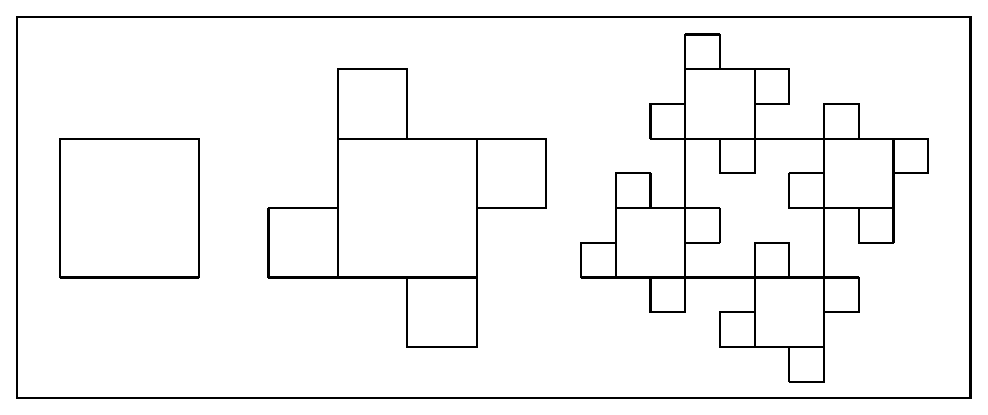
\includegraphics[width=\textwidth]{carr}

On peut d\'ecider d'avoir le dessin r\'ecursif seulement dans l'\'ecran
{\tt DispG} : le programme est plus simple car toutes les instructions 
graphiques sont ex\'ecut\'ees dans cet \'ecran.\\
On appelle cette proc\'edure {\tt carresg(a,d,f)} o\`u {\tt a} est l'affixe
du sommet en bas \`a gauche du grand  carr\'e, {\tt d} est la longueur de 
son c\^ot\'e et {\tt f} donne la longueur du c\^ot\'e du plus petit carr\'e.
{\tt carresg(a,d,f)} renvoie {\tt 1} pour que l'on puisse v\'erifier que la
proc\'edure s'est bien ex\'ecut\'ee.\\
On tape :
\begin{verbatim}
carresg(a,d,f):={
  si d>=f alors 
    carre(a,a+d);
    carresg(a-d/2,d/2,f);
    carresg(a+i*d,d/2,f);
    carresg(a+d/2-i*d/2,d/2,f);
    carresg(a+d+i*d/2,d/2,f);
  fsi;
  retourne 1;
}:;
\end{verbatim} 
On tape :
{\tt carresg(0,40,2)} \\
 L'\'ecran {\tt DispG} s'ouvre et l'on voit le dessin se faire....

On met les diff\'erentes instructions graphiques \`a r\'ealiser dans une liste
{\tt L}. On appelle cette proc\'edure {\tt carres(a,d,f)} o\`u {\tt a} est l'affixe
du sommet en bas \`a gauche du grand  carr\'e, {\tt d} est la longueur de 
son c\^ot\'e et {\tt f} donne la longueur du c\^ot\'e du plus petit carr\'e.
{\tt carresg(a,d,f)} renvoie la liste {\tt L}.\\ 
On tape :
\begin{verbatim}
carres(a,d,f):={
  local L;
  si d<f alors retourne NULL fsi;
  L:=carre(a,a+d),carres(a-d/2,d/2,f),carres(a+i*d,d/2,f),
   carres(a+d/2-i*d/2,d/2,f),carres(a+d+i*d/2,d/2,f);
  retourne L;
}
:;
\end{verbatim} 
On tape :
{\tt carres(0,40,2)} 

On peut aussi choisir comme param\`etre la profondeur {\tt n} du dessin 
r\'ecursif au lieu de {\tt f}.
On tape :
\begin{verbatim}
carren(a,d,n):={
local L;
si n=<0 alors retourne NULL fsi;
L:=carre(a,a+d),carren(a-d/2,d/2,n-1),carren(a+i*d,d/2,n-1),
   carren(a+d/2-i*d/2,d/2,n-1),carren(a+d+i*d/2,d/2,n-1);
retourne L;
}
:;
\end{verbatim} 
On tape :
{\tt carren(0,40,4)} 

\subsection{Les triangles}
On veut r\'ealiser le dessin r\'ecursif dont on a mis ci-dessous les 
premi\`eres \'etapes (profondeur 0,1,2 et 3) :

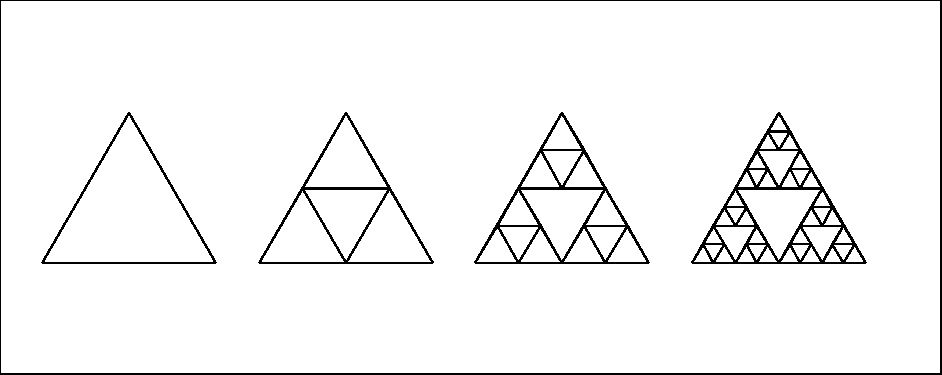
\includegraphics[width=\textwidth]{triangles}

On peut d\'ecider d'avoir le dessin r\'ecursif seulement dans l'\'ecran
{\tt DispG} : le programme est plus simple car toutes les instructions 
graphiques sont ex\'ecut\'ees dans cet \'ecran.\\
On appelle cette proc\'edure {\tt triang(a,d,f)} o\`u {\tt a} est l'affixe
du sommet en bas \`a gauche du grand  triangle, {\tt d} est la longueur de 
son c\^ot\'e et {\tt f} donne la longueur du c\^ot\'e du plus petit triangle.
{\tt triang(a,d,f)} renvoie {\tt 1} pour que l'on puisse v\'erifier que la
proc\'edure s'est bien ex\'ecut\'ee.\\
On tape :
\begin{verbatim}
triang(a,d,f):={
  si d>=f alors 
    triangle_equilateral(a,a+d);
    triang(a,d/2,f);
    triang(a+d/4+i*d*sqrt(3.)/4,d/2,f);
    triang(a+d/2,d/2,f);
  fsi;
  retourne 1;
}:;
\end{verbatim} 
On tape :
{\tt triang(0,40,2)} \\
 L'\'ecran {\tt DispG} s'ouvre et l'on voit le dessin se faire....On met les diff\'erentes instructions graphiques \`a r\'ealiser dans une liste.
On appelle cette proc\'edure {\tt triangles(a,d,f)} o\`u {\tt a} est l'affixe
du sommet  en bas \`a gauche du grand triangle, {\tt d} est la longueur de 
son c\^ot\'e et {\tt f} donne la longueur du c\^ot\'e du plus petit triangle.\\
On tape :
\begin{verbatim}
triangles(a,d,f):={
  local L;
  si d<f alors retourne NULL fsi;
  L:=triangle_equilateral(a,a+d),triangles(a,d/2,f),
     triangles(a+d/4+i*d*sqrt(3.)/4,d/2,f),triangles(a+d/2,d/2,f);
  retourne L;
}
:;
\end{verbatim} 
On tape :
{\tt triangles(0,40,2)} 

On peut aussi choisir comme param\`etre la profondeur {\tt n} du dessin 
r\'ecursif au lieu de {\tt f}.
On tape :
\begin{verbatim}
trianglen(a,d,n):={
local L;
si n<0 alors retourne NULL fsi;
L:=triangle_equilateral(a,a+d),trianglen(a,d/2,n-1),
trianglen(a+d/4+i*d*sqrt(3.)/4,d/2,n-1),trianglen(a+d/2,d/2,n-1);
retourne L;
}
:;
\end{verbatim}
On tape :
{\tt trianglen(0,40,4)} 
\subsection{Exercice}
\'Ecrire un programme qui r\'ealise le dessin r\'ecursif dont on a mis 
ci-dessous les premi\`eres \'etapes (profondeur 0, 1 et 2) :

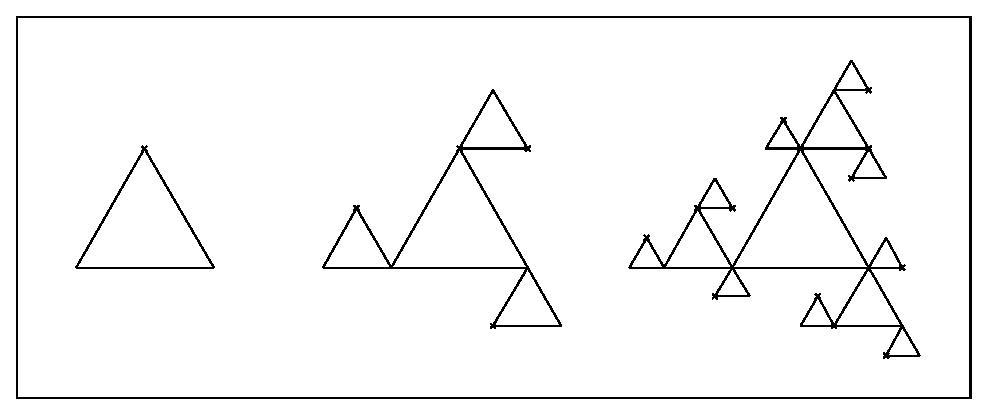
\includegraphics[width=\textwidth]{triequi}

On tape :
\begin{verbatim}
triequi(A,B,n):={
local C,L,A1,B1,C1;
L:=triangle_equilateral(A,B,C);
si n>0 alors 
A1:=homothetie(C,-0.5,A);
B1:=homothetie(A,-0.5,B);
C1:=homothetie(B,-0.5,C);
L:=L,triequi(A1,C,n-1);
L:=L,triequi(B1,A,n-1);
L:=L,triequi(C1,B,n-1);
fsi;
retourne L;
}:;
\end{verbatim}
On tape : {\tt triequi(0,1,5)}\\
On obtient :

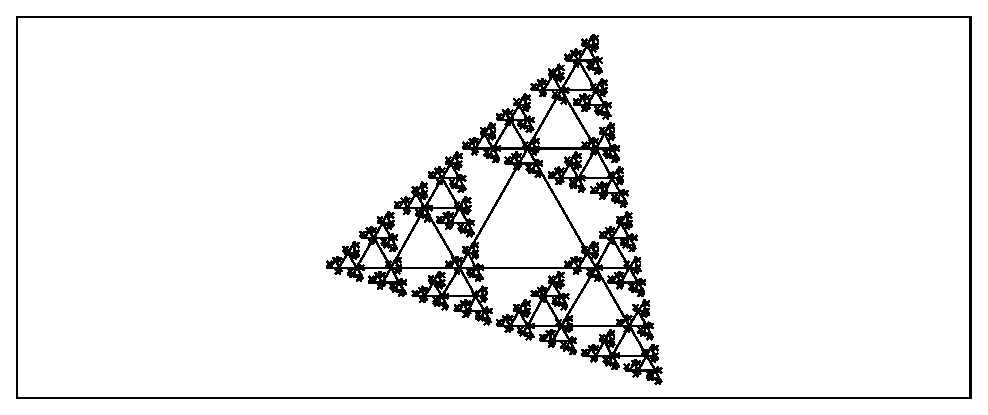
\includegraphics[width=\textwidth]{triequi5}

On tape : {\tt triequi(0,1+0.35*i,5)}\\
On obtient :

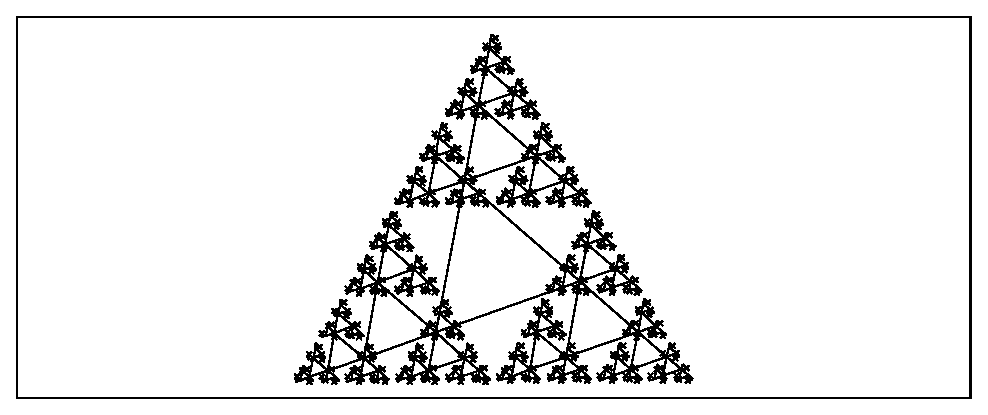
\includegraphics[width=\textwidth]{triequi55}
\subsection{Des triangles \'equilat\'eraux emboi\'es}
\`A partir d'un triangle \'equilat\`eral direct $ABC$ on construit les points 
$A_1,B_1,C_1$ v\'erifiant :\\
$\overrightarrow{AA_1}=\frac{4}{3}\overrightarrow{AB}$\\
$\overrightarrow{BB_1}=\frac{4}{3}\overrightarrow{BC}$\\
$\overrightarrow{CC_1}=\frac{4}{3}\overrightarrow{CA}$\\
Interpr\'etez $A_1$ comme le barycentre de $A,a$ et $B,b$. 
Montrer que le triangle $A_1B_1C_1$ est\'equilat\`eral.\\
On recommence la m\^eme construction \`a partir de $A_1B_1C_1$.\\
\'Ecrire la proc\'edure r\'ecursive qui r\'ealise le dessin des $n$ triangles
obtenus par cette construction (en tout $n+1$ triangles $ABC$ + les autres).\\
On a :\\
$\overrightarrow{AA_1}=\frac{4}{3}\overrightarrow{AB}-\frac{1}{3}\overrightarrow{AA}$\\
Donc $A_1$ est le barycentre de $A,-1$ et $B,4$.\\
Donc $B_1$ est le barycentre de $B,-1$ et $C,4$\\
Donc $C_1$ est le barycentre de $C,-1$ et $A,4$.\\
La rotation $r$ de centre $O$, le centre de $ABC$, et d'angle $2\pi/3$ 
transforme $A$ en $B$, $B$ en $C$ et $C$ en $A$ donc $r$ transforme le 
barycentre de $A,-1$ et $B,4$ en le barycentre de $B,-1$ et $C,4$ c'est \`a dire transforme $A_1$ en $B_1$ et  $r$ transforme le 
barycentre de $B,-1$ et $C,4$ en le barycentre de $C,-1$ et $A,4$ c'est \`a dire transforme $B_1$ en $C_1$. \\
Donc le triangle $A_1B_1C_1$ est\'equilat\`eral.\\
On tape dans l'\'editeur de programmes :
\begin{verbatim}
triangles(A,B,n):={
  local L,C;
  L:=triangle_equilateral(A,B,C);
  si n>0 alors 
    A:=barycentre([A,B],[-1,4]);
    B:=barycentre([B,C],[-1,4]);
    L:=L,triangles(A,B,n-1);
  fsi;
  return L;
}:;
\end{verbatim}
puis on compile avec {\tt F9} et dans une ligne de commande, on tape :\\
{\tt triangles(point(0),point(1),5)}
On obtient :\\
%\includegraphics[width=\textwidth]{triangle1}
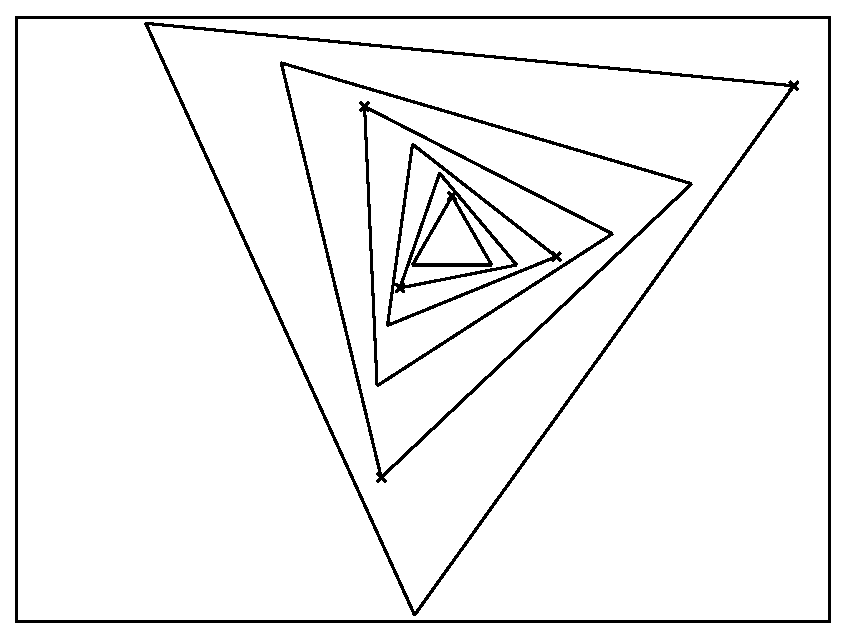
\includegraphics[width=\textwidth]{triangles1}
\subsection{Le probl\`eme des 3 insectes}
Trois insectes partent, des sommets d'un triangle 
\'equilat\'eral $A,B,C$ en direction de son voisin ($C$ regarde $B$. $B$ 
regarde $C$. $A$ regarde $C$). \`A chaque \'etape de leur 
marche les 3 insectes forment un triangle \'equilat\'eral.\\
Dessiner les trajectoires des 3 insectes en r\'esolvant une \'equation 
diff\'erentielle ou un syst\`eme d'\'equations diff\'erentielles.\\
On peut faire une simulation de la situation en supposant que chaque insecte :\\
- regarde son voisin ce qui lui donne sa direction, puis,\\
- avance dans cette direction d'une longueur proprortionnelle au c\^ot\'e du 
triangle, puis ,
- regarde son voisin ce qui lui donne sa nouvelle direction etc...\\
Faire un programme qui dessine les triangles \'etapes de cete marche.\\
Refaire le m\^eme exercice en rempla\c{c}ant le triangle 
\'equilat\'eral $A,B,C$ par un triangle rectangle isoc\`ele.\\

{\bf R\'esolution de 3 \'equations diff\'erentielles}\\
 Les trois insectes ont des trajectoires qui se d\'eduisent  l'une de l'autre 
par une rotation de centre $G$ le centre de gravit\'e du triangle et d'angle 
$-2*\pi/3$.\\ 
Si $zA$ est l'affixe du point $A$ et $zB$ celle du point $B$..., 
on a :\\
$zA'=zC-zA$\\
$zB'=zA-zB$\\
$zC'=zB-zC$\\
donc $zA'+zB'+zC'=0$ et donc \\
$zA+zB+zC=cste=1+1/2+i\sqrt 3 /2=3*zG$\\
On a :\\
$zC-zG=\exp(-2*\pi/3)(zA-zG)$ \\
$(zA-zG)'=zC-zA=(zC-zG)-(zA-zG)=(\exp(-2*\pi/3)-1)(zA-zG)$.\\
$zG=-(3+i \sqrt 3)/6$\\
au temps $t$=0 on a :
$zA=0$, $zB=1$, $zC=1/2+i \sqrt3/3$\\
On tape (on suppose que l'on a coch\'e {\tt complexe} dans la configuration du
CAS) :\\
{\tt triangle\_equlateral(0,1)}\\
{\tt zG:=(3+i*sqrt(3))/6}\\
{\tt SA:=simplify(desolve([diff(z(t),t)=(exp(-2*i*pi/3)-1)*(z(t)-zG),\\
\hspace*{3cm}z(0)=0],[t,z]))}\\
{\tt SB:=simplify(desolve([diff(z(t),t)=(exp(-2*i*pi/3)-1)*(z(t)-zG),\\
\hspace*{3cm}z(0)=1],[t,z]))}\\
{\tt SC:=simplify(desolve([diff(z(t),t)=(exp(-2*i*pi/3)-1)*(z(t)-zG),\\
\hspace*{3cm}z(0)=1/2+i*sqrt(3)/2],[t,z]))}\\
On obtient :\\
{\tt plotparam(SA[0],t=0..4),plotparam(SB[0],t=0..4),\\
plotparam(SC[0],t=0..4)}\\
On obtient :\\

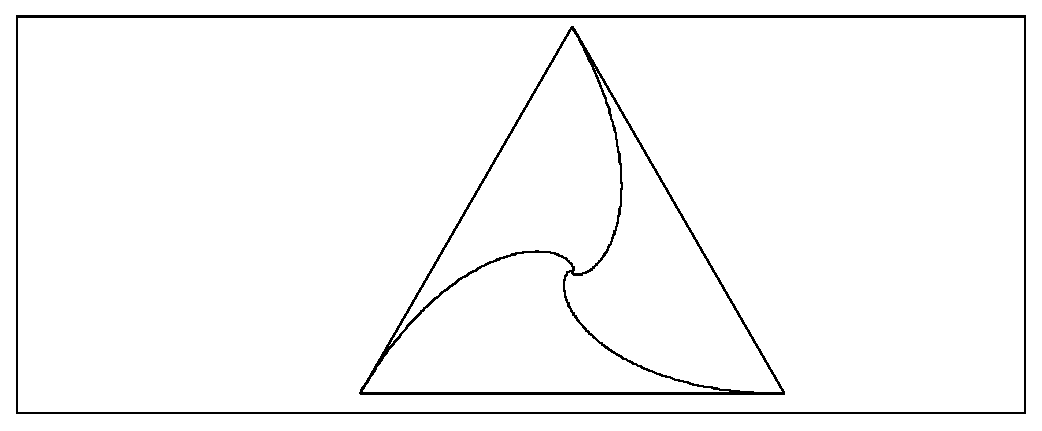
\includegraphics[width=\textwidth]{triop1}

{\bf R\'esolution d'un syst\`eme d'\'equations diff\'erentielles}\\
On peut aussi r\'esoudre le syst\`eme :\\
$Z'=A*Z$ et au temps $t=0$, $Z(0)=[0,1,1/2+i*\sqrt 3 /2]$ avec 
$$
A:=\left[\begin{array}{ccc}
-1 & 1 & 0 \\
0 & -1 & 1 \\
1 & 0 & -1
\end{array}\right]
$$ 
On tape (on suppose que {\tt Complexe} est coch\'e dans la configuration du CAS ):\\
{\tt A:=[[-1,1,0],[0,-1,1],[1,0,-1]]}\\
{\tt P,B:=jordan(A)}\\
On obtient pour $P$ :\\
{\tt [[1,(-i)*sqrt(3)-1,(i)*sqrt(3)-1],[1,2,2],[1,(i)*sqrt(3)-1,
(-i)*sqrt(3)-1]]}\\
On obtient pour $B$ :\\
{\tt [[0,0,0],[0,((i)*sqrt(3)-3)/2,0],[0,0,((-i)*sqrt(3)-3)/2]]}\\
On tape :\\
{\tt V0:=simplify(inv(P)*[0,1,1/2+i*sqrt(3)/2])}\\
On obtient :\\
{\tt [((i)*sqrt(3)+3)/6,((-i)*sqrt(3)+3)/12,0]}\\
On tape :\\
{\tt V:=V0*exp(B*t)}\\
On obtient :\\
{\tt [1/6*((i)*sqrt(3)+3),1/12*exp(((i)*sqrt(3)*t-3*t)/2)*((-i)*sqrt(3)+3),0]}\\
On tape :\\
{\tt Z:=P*V}\\
{\tt ZA:=simplify(Z[0]);ZB:=simplify(Z[1]);ZC:=simplify(Z[2]);}\\
{\tt plotparam(ZA,t=0..4),plotparam(ZB,t=0..4),plotparam(ZC,t=0..4), 
triangle\_equilateral(0,1)}\\
On obtient la figure pr\'ec\'edente.
\begin{center}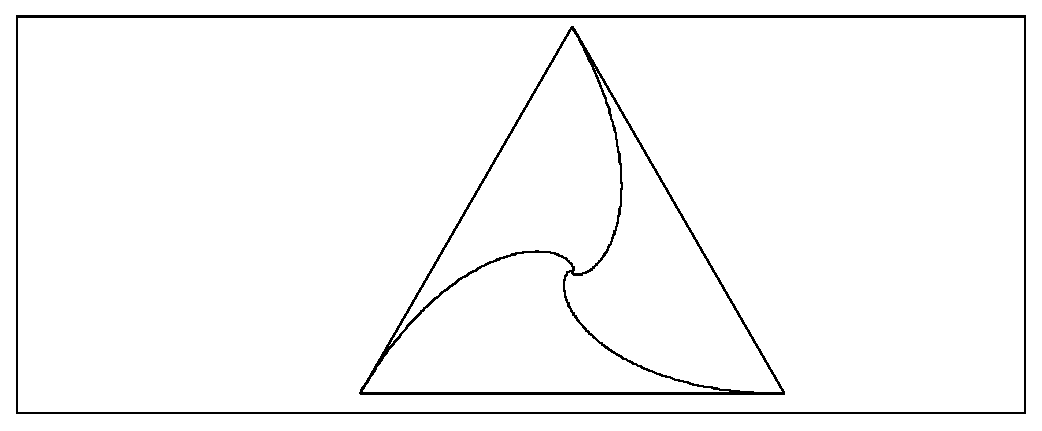
\includegraphics[width=4cm]{triop1}\end{center}
Dans le cas du triangle $ABC$ avec \\
{\tt A:=point(0)};{\tt B:=point(10)};{\tt C:=point(i*10)}, le syst\`eme \`a 
resoudre est le m\^eme c'est juste la condition initiale qui change 
({\tt V0:=inv(P)*[0,1,i]}) et les 3 
insectes convergent vers le centre de gravit\'e $K$ du triangle $ABC$.\\
On tape (on suppose que {\tt Complexe} est coch\'e dans la configuration du CAS ):\\
{\tt A:=[[-1,1,0],[0,-1,1],[1,0,-1]]}\\
{\tt P,B:=jordan(A)}\\
{\tt V0:=simplify(inv(P)*[0,1,i])}\\
On obtient :\\
{\tt [(1+i)/3,(sqrt(3)+2-i)/12,(-sqrt(3)+2-i)/12]}\\
{\tt V:=V0*exp(B*t)}\\
On obtient :\\
{\tt [(1+i)/3,1/12*exp(((i)*sqrt(3)*t-3*t)/2)*(sqrt(3)+2-i), 1/12*exp(((-i)*sqrt(3)*t-3*t)/2)*(-sqrt(3)+2-i)]}\\
On tape :\\
{\tt Z:=P*V}\\
{\tt ZA:=simplify(Z[0]);ZB:=simplify(Z[1]);ZC:=simplify(Z[2]);}\\
{\tt plotparam(ZA,t=0..4),plotparam(ZB,t=0..4),plotparam(ZC,t=0..4), 
triangle(0,1,i)}\\
On obtient la figure :\\

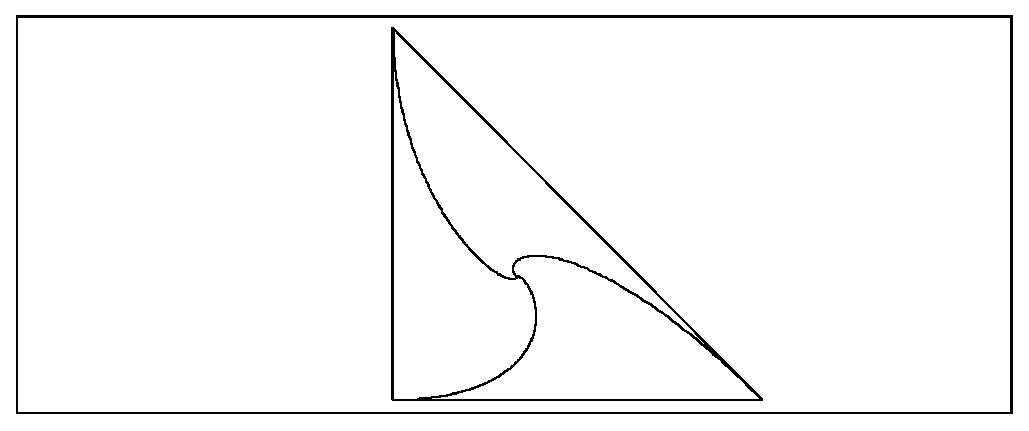
\includegraphics[width=\textwidth]{triop2}\\

{\bf Le dessin des triangles}\\
On dessine le triangle \'equilat\'eral $ABC$ puis le triangle
$A1B1C1$ avec :\\
$A1=A+\mbox{evalf}((B-A)/10)$, \\
$B1=B+\mbox{evalf}((C-B)/10)$ et\\
$C1=C+\mbox{evalf}((A-C)/10)$.\\
puis on recommence le m\^eme processus avec $A1B1C1$...
On tape :
\begin{verbatim}
triop0(a,b):={
local L,C,c;
L:=triangle_equilateral(point(a),point(b),C);
c:=evalf(affixe(C));
si evalf(abs(b-a))<1 alors return L; fsi;
a:=a*0.9+b*0.1;
b:=b*0.9+c*0.1;
L:=L,triop0(a,b);
return L;
}:;
\end{verbatim}
On tape :\\
{\tt triop0(0,10)}\\
On obtient :\\

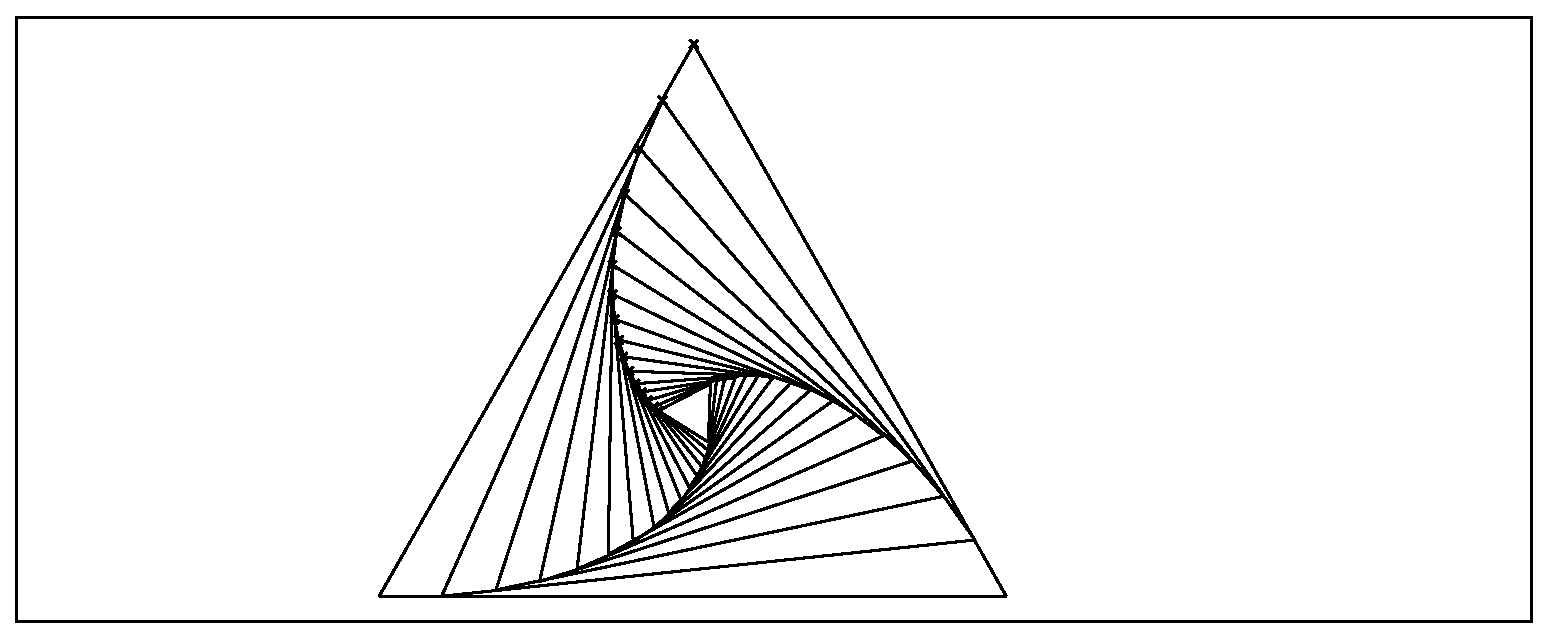
\includegraphics[width=\textwidth]{triop0}\\
On peut tourner dans l'autre sens : on dessine le triangle \'equilat\'eral 
$ABC$ puis le triangle
$A1B1C1$ avec :\\
$A1=A+\mbox{evalf}((C-A)/10)$, \\
$B1=B+\mbox{evalf}((A-B)/10)$ et\\
$C1=C+\mbox{evalf}((B-C)/10)$.\\
puis on recommence le m\^eme processus avec $A1B1C1$...
On tape :
\begin{verbatim}
triop(a,b):={
local L,C,c,a0;
L:=triangle_equilateral(point(a),point(b),C);
c:=evalf(affixe(C));
si evalf(abs(b-a))<1 alors return L; fsi;
a0:=a;
a:=a*0.9+c*0.1;
b:=b*0.9+a0*0.1;
L:=L,triop(a,b);
return L;
}:;
\end{verbatim}
On tape :\\
{\tt triop(0,10)}\\
On obtient :\\

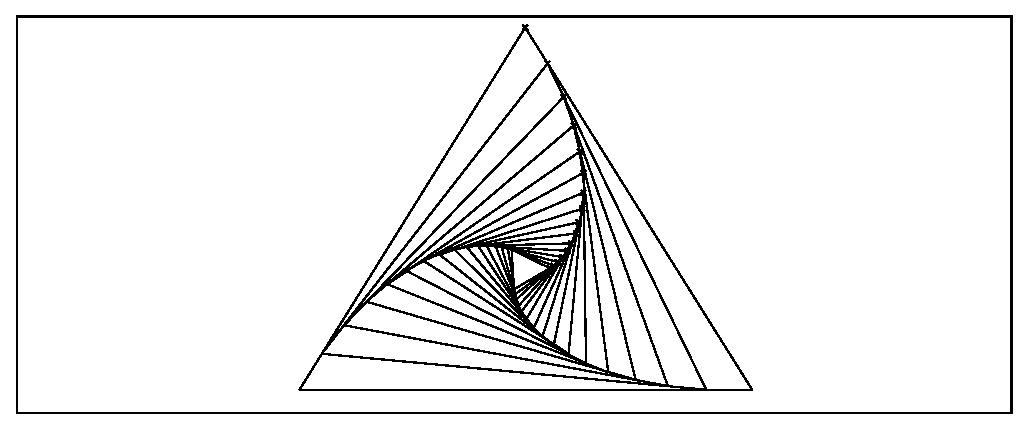
\includegraphics[width=\textwidth]{triop}\\

On tape si on choisit un triangle $ABC$ quelconque :
\begin{verbatim}
triopa(a,b,c):={
local L,a0,b0;
L:=triangle(point(a),point(b),point(c));
si (evalf(abs(b-a))<1) alors return L; fsi;
a0:=a;
b0:=b;
a:=a+evalf((c-a)/10);
b:=b+evalf((a0-b)/10);
c:=c+evalf((b0-c)/10);triopa(0,10,i*10);K:=point((10+10*i)/3)
L:=L,triopa(a,b,c);
return L;
}
:;
\end{verbatim}
On tape :\\
{\tt triopa(0,10,i*10);K:=point((10+10*i)/3)}\\
On obtient :\\

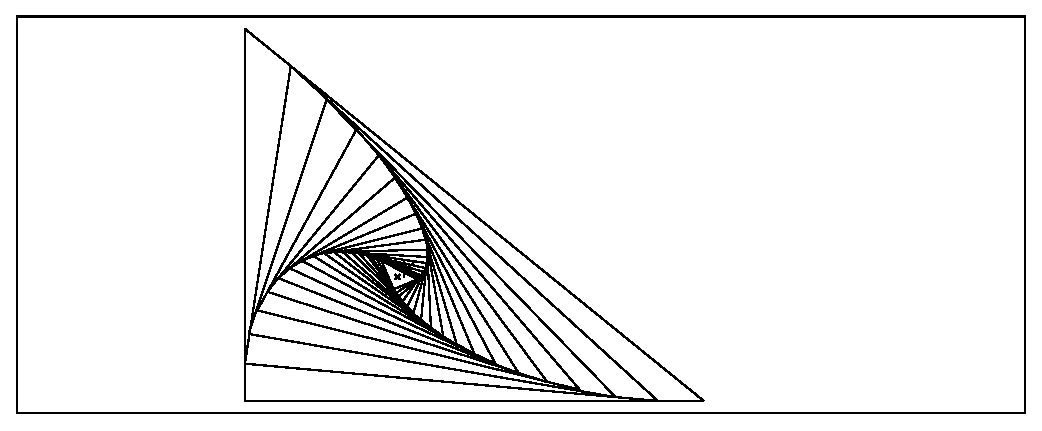
\includegraphics[width=\textwidth]{triopa}\\


{\bf On fait faire des rotations \`a ces triangles}\\
Dans triops on fait 6 rotations de {\tt triop} alors que dans {\tt triops0} on 
fait 3 rotations du losange form\'e par {\tt triop0(a,b)} et {\tt triop(b,a)}\\
0n tape :
\begin{verbatim}
triops(A,B):={
local L,j,a,b;
a:=affixe(A);
b:=affixe(B);
L:=triop0(a,b);
pour j de 1 jusque 5 faire
B:=rotation(A,pi/3,B);
b:=affixe(B);
L:=L,triop(a,b);
fpour;
return L;
}:;
triops0(A,B):={
local L,j,a,b;
a:=affixe(A);
b:=affixe(B);
L:=NULL;
pour j de 1 jusque 3 faire
L:=L,triop0(a,b),triop(b,a);
B:=rotation(A,pi/3,B);
b:=affixe(B);
fpour;
return L;
}:;
triops1(A,B):={
local L,j,a,b,c,C;
a:=affixe(A);
b:=affixe(B);
L:=NULL;
pour j de 1 jusque 3 faire
triangle_equilateral(B,A,C);
c:=affixe(C);
L:=L,triop0(a,b),triop(b,a),,triop0(a,c);
B:=rotation(A,2*pi/3,B);
b:=affixe(B);
fpour;
return L;
}:;
\end{verbatim}
On tape :\\
{\tt triops(point(0),point(10))}\\
On obtient :\\

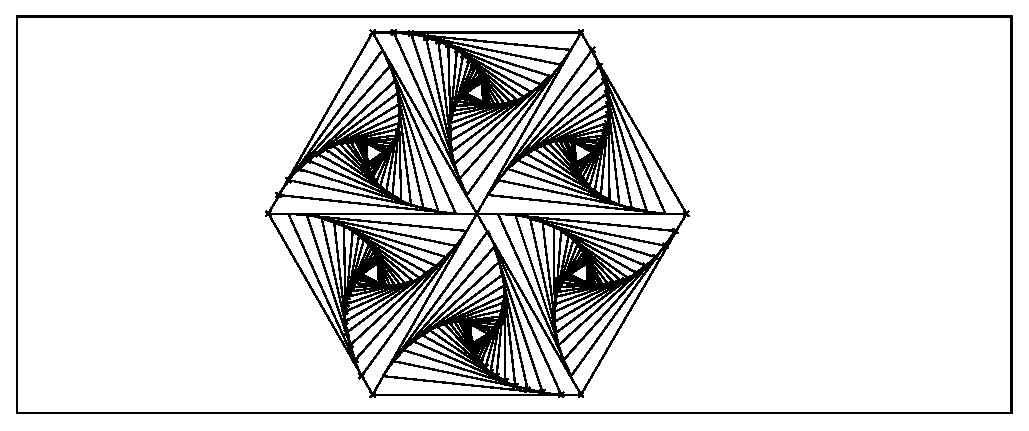
\includegraphics[width=\textwidth]{triops}
On tape :\\
{\tt triops0(point(0),point(10))}\\
On obtient :\\

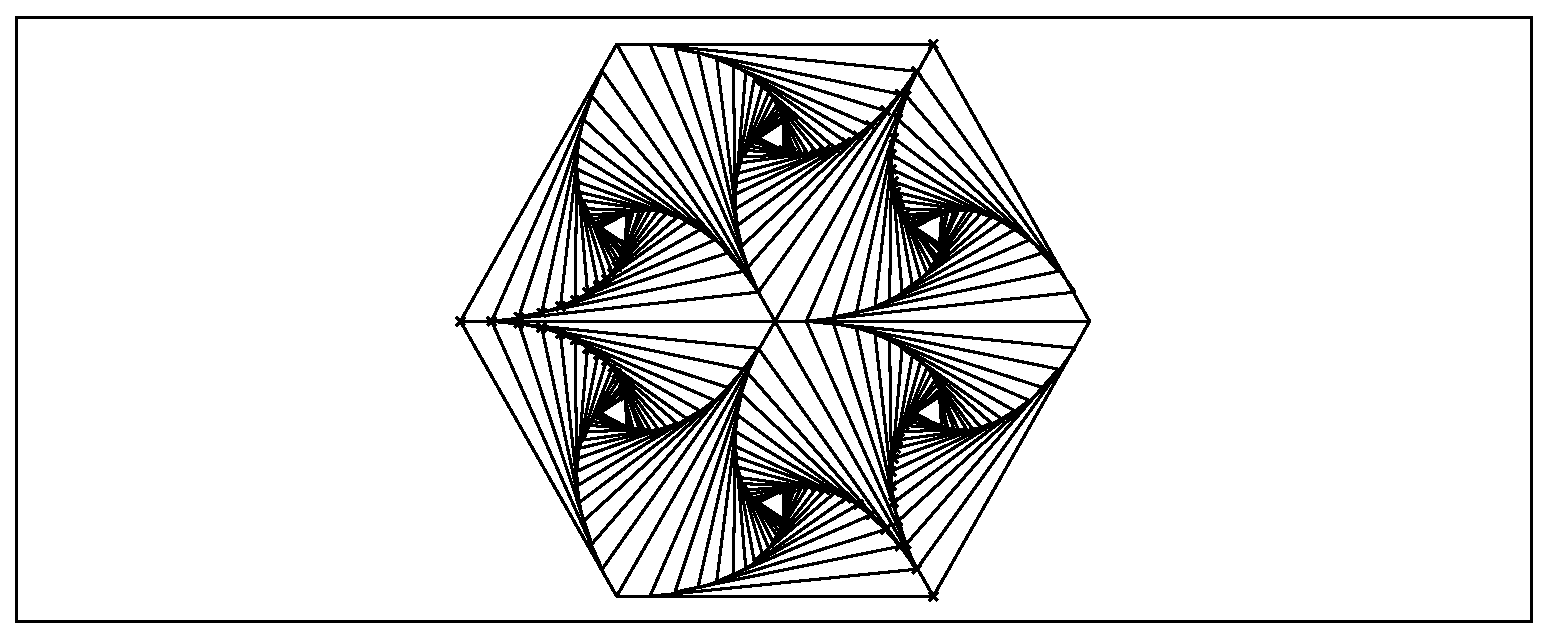
\includegraphics[width=\textwidth]{triops0}

On tape :\\
{\tt triops1(point(0),point(10))}\\
On obtient :\\

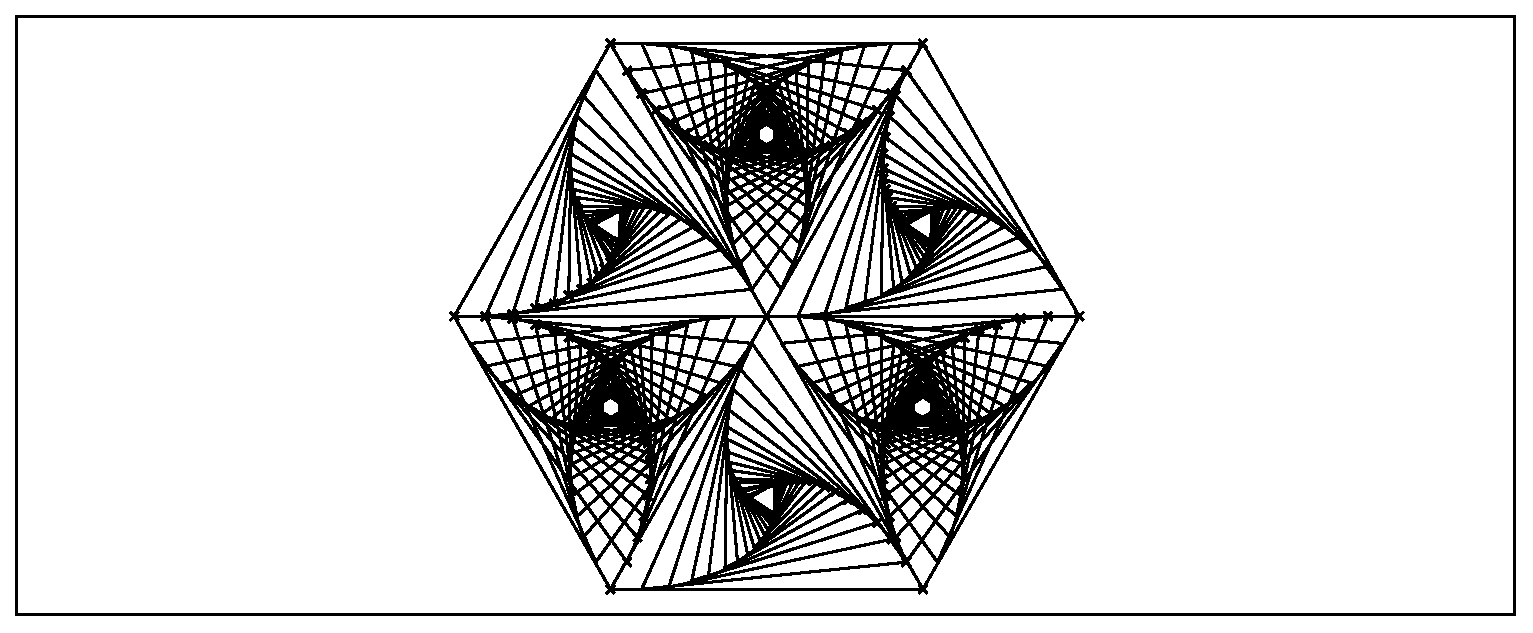
\includegraphics[width=\textwidth]{triops1}





0n tape :
\begin{verbatim}
triopas(A,B,C):={
local L,j,F,a,b,c;
a:=affixe(A);
b:=affixe(B);
c:=affixe(C);
L:=triopa(a,b,c);
pour j de 1 jusque 7 faire
A:=rotation(B,pi/4,A);
C:=rotation(B,pi/4,C);
a:=affixe(A);
c:=affixe(C);
L:=L,triopa(a,b,c);
fpour;
return L;
}:;
\end{verbatim}
On tape :\\
{\tt triopas(point(0),point(10),point(10*i))}\\
On obtient :\\

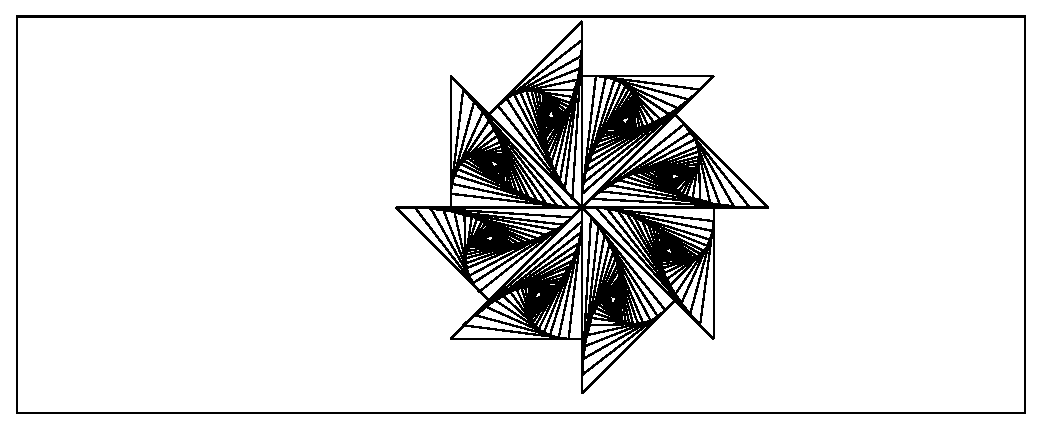
\includegraphics[width=\textwidth]{triopas}

Avec le triangle {\tt point(0),point(10),point(i*10*tan(2*pi/7))},
on tape :\\
\begin{verbatim}
triopas7(A,B,C):={
local L,j,F,a,b,c;
a:=affixe(A);
b:=affixe(B);
c:=affixe(C);
L:=triopa(a,b,c);
pour j de 1 jusque 6 faire
A:=rotation(B,2*pi/7,A);
C:=rotation(B,2*pi/7,C);
a:=affixe(A);
c:=affixe(C);
L:=L,triopa(a,b,c);
fpour;
return L;
}:;
\end{verbatim}
Puis, on tape :\\
{\tt triopas7(point(0),point(10),point(i*10*tan(2*pi/7)));}\\
On obtient :\\

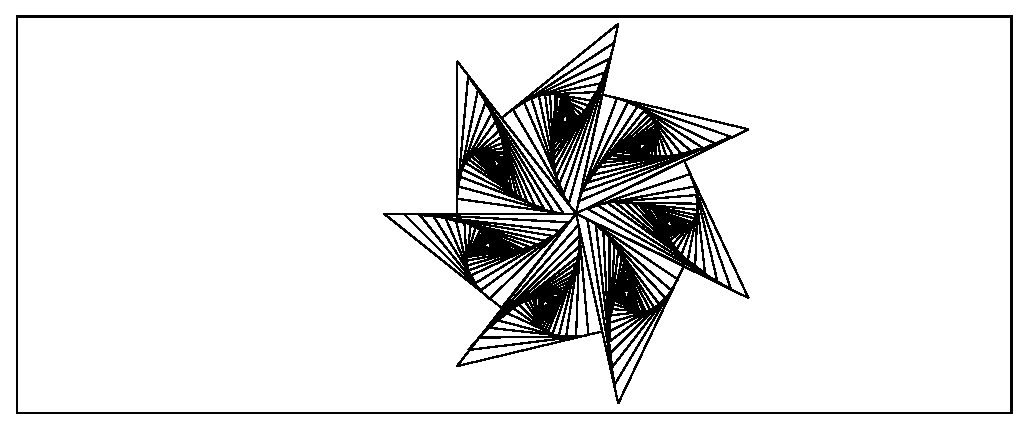
\includegraphics[width=\textwidth]{triopas7}
{\bf On peut aussi faire la m\^emes chose ave des losanges}\\
On tape :
\begin{verbatim}
losop(a,b,c,d):={
local L;
L:=quadrilatere(point(a),point(b),point(c),point(d));
si evalf(abs(b-a))<1 alors return L; fsi;
a:=a*0.9+b*0.1;
b:=b*0.9+c*0.1;
c:=c*0.9+d*0.1;
d:=d*0.9+a*0.1;
L:=L,losop(a,b,c,d);
return L;
}:;
\end{verbatim}
On tape :\\
{\tt losop(0,10,5+i*sqrt(3)*5,-5+i*sqrt(3)*5)}\\
On obtient :\\

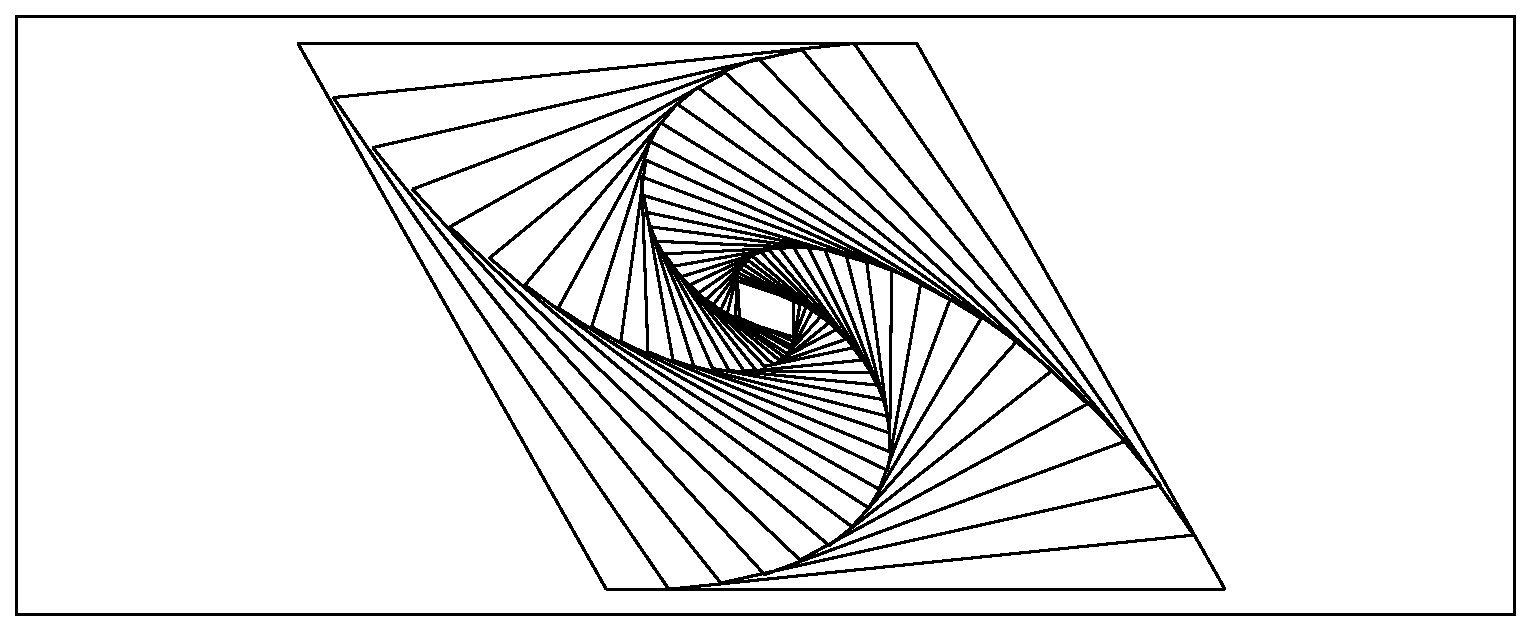
\includegraphics[width=\textwidth]{triolos}

On tape :\\
{\tt losop(10,0,-5+i*sqrt(3)*5,5+i*sqrt(3)*5),\\
losop(10,0,-5-i*sqrt(3)*5,5-i*sqrt(3)*5),\\
losop(-5+i*sqrt(3)*5,0,-5-i*sqrt(3)*5,-10)}\\
On obtient :\\

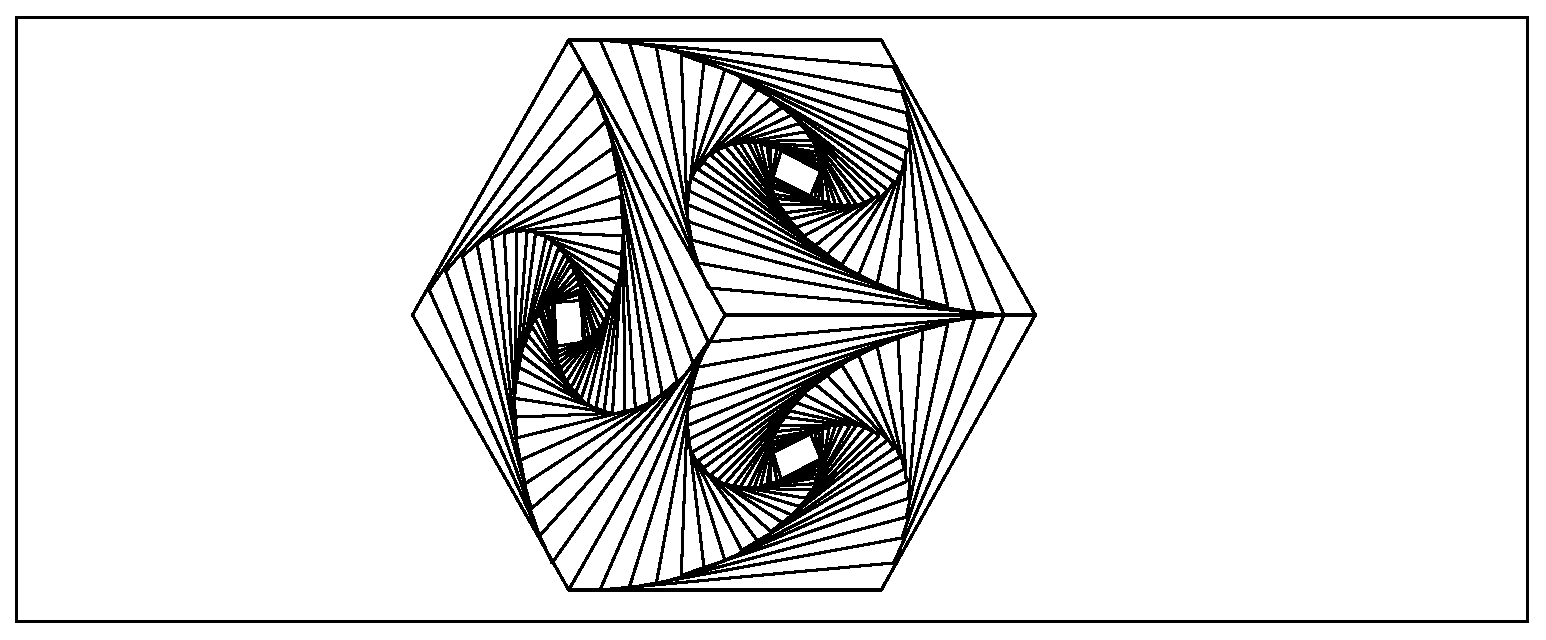
\includegraphics[width=\textwidth]{triolos3}
\subsection{Les cercles}
L'utilisateur choisit un entier {\tt n}.
Sur le cercle de de centre d'affixe {\tt a} et de rayon {\tt r} on dessine 
le cercle et les {\tt n} points d'affixe {\tt ak:=r*exp(2.*i*k*pi/n)} pour 
{\tt k=0..n-1}.
On recommence pour chaque {\tt k} avec des cercles de de centre d'affixe 
{\tt ak} et de rayon {\tt r/2}. Et ainsi de suite \`a partir des points obtenus
en divisant \`a chaque \'etape le rayon par 2.  \'Ecrire un programme qui
 r\'ealise {\tt p} \'etapes de ce processus.
On tape :
\begin{verbatim}
cercles(a,r,n,p):={
local P,L,k,j;
P:=NULL;
si p<1 alors retourne NULL fsi;
pour k de 0 jusque n-1 faire
  P:=P,point(a+r*exp(2.*i*pi*k/n),affichage=p+epaisseur_point_2);
fpour;
L:=cercle(a,r),P;
pour j de 0 jusque n-1 faire
  L:=L,cercles(affixe(P[j]),r/2,n,p-1);
fpour;
retourne L;
}:;
\end{verbatim}
On tape :\\
{\tt cercles(0,20,5,4)}\\ 
On obtient :\\

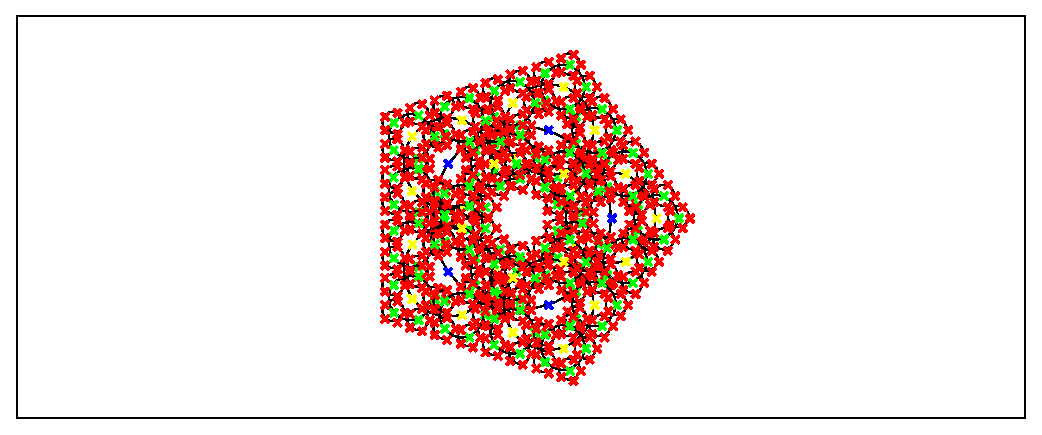
\includegraphics[width=\textwidth]{cercles}

\section{Les tours de Hano\"{i}}
Une tour de Hano\"{i} est compos\'ee de $p$ disques de rayons diff\'erents que 
l'on num\'erote de 1 \`a $p$ selon l'ordre croissant des rayons (le plus petit 
disque a le num\'ero 1 et le plus gros le num\'ero $p$).
On dispose de 3 plots num\'erot\'es de 1 \`a 3.\\
Au d\'epart les disques sont empil\'es selon l'ordre croissant sur le plot 1.\\
Le jeu consiste \`a reconstituer la tour sur le plot 2, en se servant du plot 3
comme plot interm\'ediaire, en d\'eplacant les disques un \`a un, et en posant
toujours un disque sur un disque plus petit que lui.\\
Par exemple, on peut mettre le dique 2 sur le disque 5, mais pas sur le disque 
1.\\
On veut \'ecrire un programme qui imprime ce qu'il faut faire comme 
manipulations : ce sera {\tt tour(a,b,c,p)}, o\`u {\tt p} repr\'esente le
nombre de disques, o\`u {\tt a} repr\'esente le plot 
de d\'epart, o\`u {\tt b} repr\'esente le plot d'arriv\'ee, et o\`u {\tt c} 
repr\'esente le plot interm\'ediaire.\\
On tapera alors par exemple :\\
{\tt tour(1,2,3,4)}\\
 si on a une tour de 4 disques sur le plot 1, et qu'on veut la reconstituer 
sur le plot 2 par l'interm\'ediaire du plot 3.\\
Les manipulations \`a faire sont r\'ecursives, en voici les \'etapes :
\begin{itemize}
\item iL faut arriver \`a d\'egager le disque $p$ pour qu'il soit seul sur le 
plot 1 avec les $p-1$ disques sur le plot 3, le plot 2 \'etant vide et pr\^et 
\`a recevoir le dique $p$.  Dans cette situation, il y une tour de $p-1$ 
disques sur le plot 3. Cela veut dire que l'on est arriv\'e \`a  reconstituer 
la tour constitu\'ee des $p-1$ premiers disques sur le plot 3, en se servant du
plot 2 comme plot interm\'ediaire. \\
Avec les notations ci dessus c'est que l'on a effectu\'e  :\\
{\tt tour(a,c,b,p-1)}\\
c'est l'instruction qui permet de reconstituer une tour de $p-1$ disques sur 
le plot 3 en partant du plot 1 et en se servant du plot 2 comme plot 
interm\'ediaire.\\
\item on d\'eplace ensuite le disque $p$ du plot 1 sur le plot 2 :\\
{\tt print("deplacer le disque ",p," de ", a , " vers", b)}.\\
- il reste \`a reconstituer la tour de $p-1$ disques sur le plot 2
en partant du plot 3 et en se servant du plot 1 comme plot interm\'ediaire.\\
Il faut donc effectuer :\\
 {\tt tour(c,b,a,p-1)}\\
\item il reste \`a trouver le test d'arr\^et qui est simplement {\tt (p==0)} 
c'est \`a dire  : quand on a une tour de z\'ero disque on ne fait rien 
(on renvoie 0).
\end{itemize}
On tape dans un niveau \'editeur de programmes (que l'on ouvre avec 
{\tt Alt+p}), puis on le teste et on le valide avec {\tt OK} :
\begin{verbatim}
//tour(1,2,3,4) (tour de hanoi)
//depacement des p disques (de numero 1..p du plus petit au plus grand) 
//de a vers b en passant par c
tour(a,b,c,p) :={
  if (p==0) return 0;
  tour(a,c,b,p-1);
  print("deplacer le disque "+p+" de "+ a + " vers "+ b);
  tour(c,b,a,p-1);
  return 0;
}:;
\end{verbatim} 
On tape :\\
{\tt tour(1,2,3,4)}\\
On obtient :
\begin{verbatim}
deplacer le disque 1 de 1 vers 3
deplacer le disque 2 de 1 vers 2
deplacer le disque 1 de 3 vers 2
deplacer le disque 3 de 1 vers 3
deplacer le disque 1 de 2 vers 1
deplacer le disque 2 de 2 vers 3
deplacer le disque 1 de 1 vers 3
deplacer le disque 4 de 1 vers 2
deplacer le disque 1 de 3 vers 2
deplacer le disque 2 de 3 vers 1
deplacer le disque 1 de 2 vers 1
deplacer le disque 3 de 3 vers 2
deplacer le disque 1 de 1 vers 3
deplacer le disque 2 de 1 vers 2
deplacer le disque 1 de 3 vers 2
\end{verbatim} 
\section{Les permutations}
\subsection{Les permutations circulaires}
La liste $l$ est une liste de nombres tous diff\'erents.\\
On \'ecrit la fonction {\tt circulaire(l)} qui renvoie la liste obtenue
\`a partir de  {\tt l} en renvoyant le d\'ebut de la liste {\tt l} \`a la 
fin de {\tt l}.
\begin{verbatim}
//l:=[1,2,3]; circulaire(l) 
//renvoie la liste l ou la tete est mise a la fin. 
circulaire(l):={
return concat(tail(l),l[0]);
};
\end{verbatim} 
On \'ecrit la fonction {\tt permcir(l)} qui renvoie la liste des  
permutations circulaires obtenues \`a partir de  {\tt l}. 
On \'ecrit cette fonction r\'ecursivement en renplacant  {\tt l} par
{\tt circulaire(l)}.
Il faut un test d'arr\^et pour ce parcours, pour cela on a besoin d'un 
param\`etre supplementaire qui sera {\tt ld} : c'est une liste de 
r\'ef\'erence \'egale \`a {\tt l} au d\'epart et qui n'est pas modifi\'ee. 
On s'arr\^ete quand {\tt circulaire(l)==ld}, c'est \`a dire quand on retrouve la liste de d\'epart. 
On utilise une variable 
locale {\tt lr} \'egale \`a la liste \`a renvoyer.
\begin{verbatim}
// utilise circulaire, l:=[1,2,3];permcir(l,l); 
//renvoie les permutations circulares de l
//variable locale lr la liste resultat
// ld liste reference de depart
permcir(l,ld):={
local lr;
if (circulaire(l)==ld) return [l];
lr:=[l];
lr:= append(lr,op(permcir(circulaire(l),ld)));
return lr;
};
\end{verbatim} 
 On peut supprimer la  variable locale {\tt lr} et la fonction
 {\tt circulaire}.\\
On \'ecrit alors la fonction {\tt permcc(l)} qui renvoie la liste des  
permutations circulaires obtenues \`a partir de  {\tt l}.\\
Ici, on utilise un autre test d'arr\^et, on a toujours besoin d'un 
param\`etre supplementaire qui sera {\tt ld} : c'est une liste de 
r\'ef\'erence \'egale \`a {\tt l} au d\'epart et qui est modifi\'ee, sa taille 
diminue de 1 \`a chaque appel r\'ecursif. 
On s'arr\^ete quand {\tt ld==[]}, c'est \`a dire quand on a fait autant 
d'appels que la taille de {\tt l}. 
\begin{verbatim}
//l:=[1,2,3];permcc(l,l); 
//renvoie les permutations circulares de l
//sans variable locale, ld liste reference de depart
permcc(l,ld):={
if (ld==[]) return [];
return [l,op(permcc(concat(tail(l),l[0]),tail(ld)))];
};
\end{verbatim} 
Comme il faut 2 param\`etres pour \'ecrire la fonction r\'ecursive 
{\tt permcc}, on \'ecrit la fonction finale {\tt permutation\_circ} qui 
utilise {\tt permcc} :
\begin{verbatim}
//l:=[1,2,3];permutation_circ(l); 
//renvoie les permutations circulares de l
//utilise permcc
permutation_circ(l):={
return permcc(l,l);
};
\end{verbatim} 
On tape :\\
{\tt permutation\_circ([1,2,3])}\\
On obtient :\\
{\tt [[1,2,3],[2,3,1],[3,1,2]]}

\subsection{Programme donnant toutes les permutations d'une liste $l$}
La liste $l$ est une liste de nombres tous diff\'erents.\\
1/ En faisant $n$={\tt size(l)} appels r\'ecursifs.\\
Les fonctions que l'on va \'ecrire vont utiliser la fonction {\tt echange}.
\begin{verbatim}
//echange ds l les elements d'indices j et k
echange(l,j,k):={
local a;
a:=l[j];
l[j]:=l[k];
l[k]:=a;
return l;
}:;
\end{verbatim} 

On peut d\'ecrire l'arbre des permutations de la liste $l$ :\\
\`a partir de la racine on a $n$={\tt size(l)} branches. Chaque branche
commence respectivement par chacun des \'el\'ements de la liste $l$.\\
On va donc parcourir cet arbre de la racine (n{\oe}ud de niveau 0) aux 
diff\'erentes extr\'emit\'es, en renvoyant la liste des branches parcourues 
pour arriver \`a cette extr\'emit\'e. \\
On va parcourir cet arbre en parcourant les $n$ branches. On num\'erote ces $n$
branches par $p=1..n$ et le niveau des n{\oe}uds $q=0..n-1$.\\
On aura donc $n$ appels r\'ecursifs.\\
Chaque branche $p$ ($p=1..n$) peut \^etre consid\'er\'ee \`a leur tour comme un
arbre ayant $n-1$ branches. La branche $p$ aboutit aux permutations qui laissent
invariant le $p$-i\`eme \'el\'ement de $l$ ($l[p-1]$). 
C'est cet \'el\'ement que l'on va \'echanger avec $l[0]$ pour que chaque 
branche $p$  laisse invariant l' \'el\'ement  $l[0]$.\\
On sait que l'on est arriv\'e au bout de la branche, quand on se trouve au
 n{\oe}ud de niveau $n-1$, dans ce cas la permutation chech\'ee est $l$ (c'est 
la permutation obtenue \`a partir de $l$ en laissant ces $n-1$ premiers 
\'el\'ements invariants).\\
On utilise une variable locale {\tt lr}, \'egale \`a la liste \`a renvoyer et 
un param\`etre {\tt k}, pour que {\tt permus(l,k)} renvoie toutes les 
permutations de {\tt l} qui laissent invariant les k premiers \'el\'ements de 
{\tt l}. On tape :
\begin{verbatim}
//utilise echange et la variable locale lr (liste resultat)
//permus(l,k) laisse invariant les k premiers elements de l
//permus([1,2,3,4],0); renvoie toutes les permutations de l 
permus(l,k):={
local lr,j;
if (k==size(l)-1) return [l];
lr:=[];
for (j:=k;j<size(l);j++){
l:=echange(l,k,j);
lr:=[op(lr),op(permus(l,k+1))];
l:=echange(l,j,k);
}
return lr;
}:;
\end{verbatim} 
On n'est pas oblig\'e de remettre la suite $l$ \`a sa valeur de d\'epart
pour recommencer l'it\'eration puisque le premier \'echange dans l'it\'eration 
revient \`a transformer $l$ en la liste o\`u on a mis son $j$-i\`eme 
\'el\'ement en t\^ete ($j=0..n-1$). La liste r\'esultat ne sera alors pas dans 
le m\^eme ordre. Si on veut avoir la liste dans l'ordre lexicographique, il ne 
faut pas mettre la deuxi\`eme instruction {\tt echange}. En effet :\\
 sans la deuxi\`eme instruction {\tt echange}, on \'echange
0 et 1 pour j=1 ([1,0,2..]) puis 0 et 2  pour j=2 ([2,0,1..]) etc
 sans la deuxi\`eme instruction {\tt echange}, on \'echange
0 et 1 ([1,0,2..]) puis, 1 et 0 ([0,1,2..]) pour j=1, puis
0 et 2 ([2,1,0..]) puis, 2 et 0 ([0,1,2..]) pour j=2 etc
\begin{verbatim}
//permuts([1,2,3,4],0) utilise echange 
//la 2ieme instruction echange est inutile
permuts(l,k):={
local lr,j;
if (k==size(l)-1) return [l];
lr:=[];
for (j:=k;j<size(l);j++){
l:=echange(l,k,j);
lr:=[op(lr),op(permuts(l,k+1))];
}
return lr;
}:;
\end{verbatim} 
Comme il faut 2 param\`etres pour \'ecrire la fonction r\'ecursive 
{\tt permuts}, on \'ecrit la fonction {\tt permutation} qui utilise 
{\tt permuts}:
\begin{verbatim}
//l:=[1,2,3];permutation(l); 
//renvoie toutes les permutations de l
//utilise permuts
permutation(l):={
return permuts(l,0);
};
\end{verbatim} 
On tape :\\
{\tt permutation([1,2,3])}\\
On obtient :\\
{\tt [[1,2,3],[1,3,2],[2,1,3],[2,3,1],[3,1,2],[3,2,1]]}\\
On peut aussi \'ecrire une autre fonction r\'ecursive ayant comme param\`etre 
{\tt ld} et {\tt lf}. {\tt ld} contient les premi\`eres valeurs de {\tt l} qui 
seront inchang\'ees dans la permutation et {\tt lf}  contient les valeurs
restantes de {\tt l}, celles qui restent \`a permuter. On remarquera que le 
r\'esultat mis dans {\tt res} est ici une s\'equence. 
\begin{verbatim}
//au debut ld=[] et lf=l,
//groupe_s([],l) renvoie toutes les permutations de l
groupe_s(ld,lf):={
 local j,n,res;
 n:=size(lf);
 res:=NULL;
 if (n==1)
   return concat(ld,lf);
 for (j:=0;j<n;j++){
   res:=res,groupe_s(append(ld,lf[0]),tail(lf));
   // permutation circulaire
   lf:=append(tail(lf),lf[0]);
 }
 return res;
};
\end{verbatim} 
Et la fonction {\tt groupesym} qui utilise la fonction r\'ecursive 
{\tt groupe\_s} :
\begin{verbatim}
//utilise groupe_s
//groupesym(l) renvoie toutes les permutations de l
groupesym(l):=return(groupe_s([],l));
\end{verbatim} 
2/ En faisant $2$ appels r\'ecursifs.\\
Cet algorithme est surtout fait pour des langages qui n'ont pas de boucle 
{\tt for}.\\
Les fonctions vont utiliser la fonction {\tt circulaire} (pour plus de 
claret\'e), puis on remplacera {\tt circulaire(l)} par 
{\tt concat(tail(l),l[0])}.
\begin{verbatim}
//l:=[1,2,3]; circulaire(l) 
//renvoie la liste l ou la tete est mise a la fin. 
circulaire(l):={
return concat(tail(l),l[0]);
};
\end{verbatim} 
On peut d\'ecrire l'arbre des permutations de la liste $l$ :\\
\`a partir de la racine on a $n$={\tt size(l)} branches. Chaque branche
 commence par chacun des \'el\'ements de la liste $l$.\\
On va parcourir cet arbre, en parcourant la premi\'ere branche, puis en 
consid\'erant qu'il reste \`a parcourir un arbre de $n-1$ branches.\\
On aura donc 2 appels r\'ecursifs.\\
Pour le parcours de la premi\`ere branche, il faut connaitre la liste des 
\'el\'ements qui nous a permis d'arriver \`a un n{\oe}ud donn\'e, c'est cette 
liste que l'on met dans {\tt ldl}, {\tt l} contenant les \'el\'ements qu'il 
faut encore permuter. On s'arr\^ete quand {\tt l=[]}, et le r\'esultat est 
{\tt [ldl]}.\\
Pour le parcours des $n-1$ branches restantes, on change pour chaque branche
la liste \`a permuter en {\tt circulaire(l)}.\\
Il faut un test d'arr\^et pour ce parcours, pour cela on a besoin d'un 
param\`etre supplementaire qui sera {\tt ld} (liste de r\'ef\'erence \'egale 
\`a {\tt l} au d\'epart) dans {\tt permss} ou qui sera 
{\tt n} (longueur de {\tt l} au d\'epart) dans {\tt permss1}.\\
On \'ecrit {\tt permss} :
\begin{verbatim}
// utilise circulaire, l:=[1,2];permss([],l,l);
//ldl=debut de l, l=liste a permuter, 
//ld=liste de reference (=l au debut)
permss(ldl,l,ld):={
if (l==[]) return [ldl];
if (ld==[]) return ld;
return [op(permss(concat(ldl,l[0]),tail(l),tail(l))),
        op(permss(ldl,circulaire(l),tail(ld)))];
};
\end{verbatim} 
On \'ecrit {\tt permss1} qui utilise comme param\`etre {\tt n} qui
repr\'esente la longueur de la liste qui reste \`a permuter ({\tt n=size(l)} au d\'epart) :\\
\begin{verbatim}
//utilise circulaire, l:=[1,2,3,4];permss1([],l,size(l)); 
//ldl=debut de l, l=liste a permuter, n=size(l) au debut
permss1(ldl,l,n):={
if (l==[]) return [ldl];
if (n==0) return [];
return [op(permss1(concat(ldl,l[0]),tail(l),size(tail(l)))),
        op(permss1(ldl,circulaire(l),n-1))];
};
\end{verbatim} 
On a aussi \'ecrit la fonction {\tt permss2} contenant une variable locale
{\tt lr} qui est la liste \`a renvoyer et qui donne un algorithme plus lisible.
\begin{verbatim}
//l:=[1,2];permss2([],l,l); 
//ldl=debut de l, l=liste a permuter,
//ld=liste de reference (=l au debut)
// lr liste a renvoyer en variable locale
permss2(ldl,l,ld):={
local lr;
if (l==[]) return [ldl];
if (ld==[]) return [];
lr:=permss2(concat(ldl,l[0]),tail(l),tail(l));
lr:=append(lr,op(permss2(ldl,concat(tail(l),l[0]),tail(ld))));
return lr
};
\end{verbatim} 
puis la fonction {\tt permute} qui utilise {\tt permss2} :
\begin{verbatim}
//utilise permss2, 
//permute(l) renvoie toutes les permutations de l
permute(l):={
return permss2([],l,l);
};
\end{verbatim} 
On tape :\\
{\tt permute([1,2,3])}\\
On obtient :\\
{\tt [[1,2,3],[1,3,2],[2,3,1],[2,1,3],[3,1,2],[3,2,1]]}

\chapter{R\'ecup\'erer et installer un logiciel}
La description qui suit s'applique au navigateur Netscape. Elle
s'applique de mani\`ere identique pour d'autres navigateurs \`a
quelques d\'etails pr\`es.

Lorsqu'un lien mentionne un logiciel que vous voulez t\'el\'echarger, 
maintenez la touche Shift appuy\'ee et cliquez avec la souris sur
ce lien. Une fen\^etre s'ouvre et vous propose de sauvegarder
un fichier sur votre disque dur, changez \'eventuellement le nom
de ce fichier et notez l'emplacement du r\'epertoire o\`u il a \'et\'e
sauvegard\'e.

La m\'ethode d'installation du logiciel d\'epend de votre syst\`eme d'exploitation
et du type de fichier t\'el\'echarg\'e, que l'on d\'etermine en g\'en\'eral par
son extension, c'est-\`a-dire par les lettres (en principe 3) qui
suivent le caract\`ere point dans le nom de ce fichier.

Sous Windows, vous r\'ecup\'ererez en g\'en\'eral un fichier ex\'ecutable \verb|exe|
il suffit alors de cliquer sur son ic\^one pour installer le logiciel.
Ou alors il s'agira d'une archive, il vous faudra alors un logiciel
de d\'ecompression pour l'installer (l'un des plus populaires s'appelle
Winzip et propose une version \`a l'essai gratuitement). Une fois
d\'esarchiv\'e votre logiciel, vous trouverez dans l'archive un fichier
donnant des instructions compl\'ementaires ou vous devrez vous r\'ef\'erer
au site o\`u vous avez t\'el\'echarg\'e l'archive.

Sous Linux, les formats les plus courants sont \verb|rpm|,
\verb|deb| et \verb|tgz| (ou \verb|tar.gz|).

Les deux premiers correspondent \`a des distributions Linux (Red Hat,
Mandrake, Suse par exemple pour \verb|rpm|, Debian pour \verb|deb|)
ils doivent \^etre install\'es par \verb|root| (tapez \verb|su|
dans une fen\^etre de commandes pour passer \verb|root|)
en utilisant respectivement les commandes:\\
\verb|rpm -U nom_de_fichier.rpm| pour Red Hat, Mandrake, Suse\\
\verb|apt-get install nom_de_fichier_deb| pour Debian\\
Regardez bien les \'eventuels messages d'erreurs qui apparaissent. Ils
peuvent signaler que vous devez installer d'autres logiciels de votre
distribution Linux pour faire fonctionner votre nouveau logiciel.
En g\'en\'eral ces logiciels non install\'es se trouvent sur le CD-ROM
de votre distribution Linux. Ils s'installent par la m\^eme commande,
mais vous devrez d'abord vous d\'eplacer dans le r\'epertoire du CD-ROM
qui les contient. Pour cela, introduisez le CD-ROM dans le lecteur,
attendez quelques secondes, tapez : \verb|ls /mnt/cdrom|\\
(si rien n'apparait, tapez : \verb|mount /mnt/cdrom| et recommencez). \\
Ensuite tapez \verb|cd /mnt/cdrom| puis allez dans
le r\'epertoire correct (par exemple \verb|cd Mandrake/RPMS| pour
une distribution Mandrake) et lancez les commandes d'installation
des logiciels manquants (\verb|rpm -U ...| ou \verb|apt ...|).
Certaines distributions Linux proposent des interfaces plus ou moins
conviviales pour installer des logiciels, par exemple \verb|rpmdrake|
pour Mandrake, \verb|dselect| pour Debian...

Les archives \verb|tar.gz| et \verb|tgz| s'installent 
sur toute distribution Linux. Commencez par en
regarder la table des mati\`eres par la commande:\\
\verb|tar tvfz nom_de_fichier.tgz|\\
afin de d\'eterminer depuis quel r\'epertoire il faut d\'ecompacter le fichier
ou lisez la documentation du logiciel disponible en g\'en\'eral sur le site
o\`u vous avez t\'el\'echarg\'e l'archive.
Si vous voyez apparaitre des chemins tels que \verb|usr/local/bin| ou
\verb|usr/bin|, placez vous dans le r\'epertoire racine (\verb|cd /|)
puis tapez:\\
\verb|tar xvfz nom_du_repertoire/nom_de_fichier.tgz|\\
(si vous avez sauvegard\'e l'archive dans votre r\'epertoire, vous pouvez
utiliser :\\
\verb|~votre_nom_de_login| comme \verb|nom_de_repertoire|),\\
sinon, tapez simplement depuis le r\'epertoire o\`u se trouve l'archive:\\
\verb|tar xvfz nom_de_fichier.tgz|\\
placez-vous dans le r\'epertoire cr\'e\'e et lisez les fichiers \verb|README|
ou/et \verb|INSTALL| qui s'y trouvent sans doute.\\
Remarques :
 
1/ N'oubliez pas de quitter le compte de \verb|root| avant
d'utiliser votre logiciel (en tapant simultan\'ement sur les touches
Ctrl et D).

2/ les archives \verb|.tar.bz2| se traitent de mani\`ere identique,
\`a ceci pr\`es qu'il faut enlever le \verb|z| de \verb|tvfz| ou \verb|xvfz|
et rajouter \\
\verb| --use-compress-program bunzip2|, par exemple:\\
\verb|tar tvf nom_de_fichier.tar.bz2 --use-compress-program bunzip2|

3/ les archives \verb|.zip| se visualisent par la commande :\\
\verb|unzip -v nom_de_fichier.zip| et se d\'esarchivent par la commande :\\
\verb|unzip nom_de_fichier.zip|

Sous linux et autres Unix, vous trouverez \'egalement des fichiers
sources qu'il vous faudra compiler avant de pouvoir utiliser le logiciel
correspondant. De nombreux fichiers sources suivent la proc\'edure
d'installation du projet GNU. Pour les compiler la proc\'edure est
la suivante (apr\`es avoir d\'ecompress\'e l'archive):\\
\verb|cd nom_d_archive|\\
\verb|./configure|\\
\verb|make|\\
Puis on passe \verb|root| en tapant \verb|su|, puis : \verb|make install-strip|\\
puis quittez le compte \verb|root| (en tapant simultan\'ement 
sur les touches \verb|Ctrl| et \verb|D|).
Vous pourrez alors utiliser le logiciel nouvellement install\'e 
(\'eventuellement
apr\`es avoir tap\'e la commande \verb|rehash| si votre interpr\'eteur de
commandes est \verb|tcsh|).

Si cela ne fonctionne pas vous devriez trouver un fichier \verb|README|
ou \verb|INSTALL| qui explique la proc\'edure \`a suivre.
\newpage
\printindex
\newpage
\tableofcontents
\end{document}
\begin{verbatim}
urec(f,n,l0):={
local s,k,uk;
s:=size(l0);
//f est une fonction de s variables
for (k:=s;k<=n;k++) {
uk:=f(op(l0));
l0:=concat(tail(l0),uk);
}
return uk;
}
\end{verbatim}

\begin{verbatim}
f1(k,acc):={
local prod,j;
prod:=1/(k+1);
for (j:=2;j<=acc+1;j++){
prod:=prod/(k+j);
}
return prod;
}
serie_sumacc(f1,n,acc):={
local l,j,ls,prod,g,f,p,sf,sg;
purge(k);
f(k):=1/(k+1)^2;
f0:=f;
p:=2;
ls:=[serie_sum(f,0,n)];\\
for (j:=1;j<=acc;j++) {
g(k):=f(k)-f1(k,j);
sf:=serie_sum(f0,0,j-1);
sg:=serie_sum(g,0,n);
ls:=concat(ls,serie_sum(f0,0,j-1)+serie_sum(g,0,n));
f:=g;
}
return(ls);
}
\end{verbatim} 
avec la fonction $g$ algo analyse
\begin{verbatim}
f1(k,acc):={
local prod,j;
prod:=1/(k+1);
for (j:=2;j<=acc+1;j++){
prod:=prod/(k+j);
}
return prod;
};
serie_sumacc(f1,n,acc):={
local l,j,jf,ls,prod,g,f,p,sf,sg;
purge(k);
f(k):=1/(k+1)^2;
f0:=f;
p:=2;
ls:=[serie_sum(f,0,n)];\\
for (j:=1;j<=acc;j++) {
f1j(k):=f1(k,j)
g:=f-f1j;
sf:=serie_sum(f0,0,j-1);
sg:=serie_sum(g,0,n);
ls:=concat(ls,sf+sg);
f:=g;
}
return(ls);
}
serie_sumacc(f1,n,acc):={
local l,j,jf,ls,prod,g,f,p,sf,sg;
purge(k);
f(k):=1/(k+1)^2;
f0:=f;
p:=2;
ls:=[serie_sum(f,0,n)];\\
for (j:=1;j<=acc;j++) {
f1j:=(k)->f1(k,j)
g:=(k)->f(k)-f1j(k);
sf:=serie_sum(f0,0,j-1);
sg:=serie_sum(g,0,n);
ls:=concat(ls,sf+sg);
p:=p+1;
f:=g;
}return(ls);
}
\end{verbatim}

\begin{verbatim}
seriealt_sumacc(n,acc):={
local l,j,k,ls,sf,sg,gk,fact2,alt,t0,p;
//calcul sans acceleration
sf:=0.0;
alt:=1;
for (k:=n;k>=0;k--) {
sf:=sf+alt/(k+1);
alt:=-alt;
}
if (alt==1) {
ls:=[-sf];} 
else {
ls:=[sf];
}
t0:=0.5;
sf:=0.0;
fact2:=1;
for (p:=1;p<=acc;p++){
  //calcul de p!/2^p dans fact2
  sf:=sf+fact2*t0;
  fact2:=fact2*(p)/2;
  //calcul de sg, somme(de 0 a n) de la serie gk acceleree p fois
  sg:=0.0;
  //calcul du terme g0 de la serie acceleree p fois (sans p!/2^p)
  gk:=1;
  for (j:=1;j<=p;j++) {
    gk:=evalf(gk/(j+1));
  }
  t0:=gk/2;
  sg:=sg+gk;
  alt:=-1;
  for (k:=1;k<=n;k++) {
     gk:=1/(k+1);
     //calcul du k-ieme terme gk de la serie acceleree p fois (sans p!/2^p)
     for (j:=1;j<=p;j++) {
       gk:=evalf(gk/(k+j+1));
     }
     sg:=sg+alt*gk;
     alt:=-alt;
  } 
ls:=concat(ls,sf+fact2*sg);
}
return(ls);
}
\end{verbatim}

\begin{verbatim}
gauss_reducni(M):={
local pivo,j,k,jj,kk,nl,nc,temp,l,n,a,piv,kpiv,maxi;
nl:=nrows(M);
nc:=ncols(M);
n:=min(nl,nc-1);
//on met des 0 sous la diagonale du carre n*n
for (j:=0;j<n;j++) {
   //on normalise les lignes
   for (jj:=0;jj<nl;jj++) {
       maxi:=max(abs(seq(M[jj,kk], kk=0..nc-1)));
       for (kk:=0;kk<nc;kk++) {
           M[jj,kk]:=M[jj,kk]/maxi;
       }  
   }
//choix du pivot
    kpiv:=j;
    piv:=abs(M[kpiv,j]);
    for (k:=j+1;k<nl;k++){
    if (abs(M[k,j])>piv) {piv:=abs(M[k,j]);kpiv:=k;}
    }
   //on ne fait la suite que si on a piv!=0
    if (piv!=0) {
      pivo:=M[kpiv,j];
      k:=kpiv;
      //echange de la ligne j et de la ligne k
      for (l:=j;l<nc;l++){
       temp:=M[j,l];
       M[j,l] := M[k,l];
        M[k,l]:=temp;     
      }
     //fin du choix du pivot qui est M[j,j]
     for (k:=j+1;k<nl;k++) {
        a:=M[k,j];
        for (l:=j;l<nc;l++){ 
          M[k,l]:=M[k,l]-M[j,l]*a/pivo; 
         } 
       }
    }  
}
return M;
};
\end{verbatim} 

\begin{verbatim}
gauss_reducn(M):={
local pivo,j,jc,jl,k,nl,nc,temp,l,a,piv,kpiv,maxi;
nl:=nrows(M);
nc:=ncols(M);
//on met des 0 sous la diagonale
while (jc<nc-1 and jl<nl-1) {
    //on normalise les lignes
    for (jj:=0;jj<nl;jj++) {
       maxi:=max(abs(seq(M[jj,kk], kk=0..nc-1)));
       for (kk:=0;kk<nc;kk++) {
          M[jj,kk]:=M[jj,kk]/maxi;
       }  
    }
    //choix du pivot
    kpiv:=jl;
    piv:=abs(M[kpiv,jc]);
    for (k:=jl+1;k<nl;k++){
    if (abs(M[k,jc])>piv) {piv:=abs(M[k,jc]);kpiv:=k;}
    }
   //on ne fait la suite que si on a piv!=0
    if (piv!=0) {
      pivo:=M[kpiv,jc];
      k:=kpiv;
      //echange de la ligne jl et de la ligne k
      for (l:=jc;l<nc;l++){
       temp:=M[jl,l];
       M[jl,l] := M[k,l];
        M[k,l]:=temp;     
      }
     //fin du choix du pivot qui est M[jl,jc]
     //on met des 0 sous la fausse diagonale de la colonne jc
       for (k:=jl+1;k<nl;k++) {
        a:=M[k,jc];
        for (l:=jc;l<nc;l++){ 
          M[k,l]:=M[k,l]-M[jl,l]*a/pivo; 
         } 
       }
      //on a un pivot,le numero de ligne de la fausse diag augmente de 1
      jl:=jl+1;
    }
    //ds tous les cas,le numero de colonne de la fausse diag augmente de 1
    jc:=jc+1;  
}
return M;
};
\end{verbatim} 

\begin{verbatim} 
gaussjordan_reducni(M):={
local pivo,j,k,nl,nc,temp,l,n,a,piv,kpiv,maxi;
nl:=nrows(M);
nc:=ncols(M);
n:=min(nl,nc-1);
//on met des 0 sous la diagonale du carre n*n
for (j:=0;j<n;j++) {
    //on normalise les lignes
    for (jj:=0;jj<nl;jj++) {
      maxi:=max(abs(seq(M[jj,kk], kk=0..nc-1)));
      for (kk:=0;kk<nc;kk++) {
        M[jj,kk]:=M[jj,kk]/maxi;
      }  
    } 
    //choix du pivot
    kpiv:=j;
    piv:=abs(M[kpiv,j]);
    for (k:=j+1;k<nl;k++){
    if (abs(M[k,j])>piv) {piv:=abs(M[k,j]);kpiv:=k;}
    }
   //on ne fait la suite que si on a piv!=0
    if (piv!=0) {
      pivo:=M[kpiv,j];
      k:=kpiv;
      //echange de la ligne j et de la ligne k
      for (l:=j;l<nc;l++){
       temp:=M[j,l];
       M[j,l] := M[k,l];
        M[k,l]:=temp;     
      }
     //fin du choix du pivot qui est M[j,j]
      for (k:=0;k<j;k++) {
        a:=M[k,j];
        for (l:=0;l<nc;l++){ 
          M[k,l]:=M[k,l]-M[j,l]*a/pivo; 
         } 
      }
      for (k:=j+1;k<nl;k++) {
        a:=M[k,j];
        for (l:=j;l<nc;l++){ 
          M[k,l]:=M[k,l]-M[j,l]*a/pivo; 
         } 
       }
    }  
}
return M;
}
\end{verbatim}
\begin{verbatim}     
gaussjordan_noyau(M):={
local pivo,jc,k,j,nl,nc,temp,l,a,noyau;
nl:=nrows(M);
nc:=ncols(M);
//on met des 0 sous la diagonale 
jc:=0;
// on traite toutes les colonnes
while (jc<nc and jc<nl) {
  //choix du pivot que l'on veut mettre en M[jc,jc]
    k:=jc;
    while (M[k,jc]==0 and k<nl-1) {k:=k+1;}
    //on ne fait la suite que si on a pivo!=0
    if (M[k,jc]!=0) {
      pivo:=M[k,jc];
      //echange de la ligne jc et de la ligne k
      for (l:=jc;l<nc;l++){
       temp:=M[jc,l];
       M[jc,l] := M[k,l];
        M[k,l]:=temp;     
      }
     //fin du choix du pivot qui est M[jc,jc]
      //on met 1 sur la diagonale de la colonne jc
      for (l:=0;l<nc;l++) {
      M[jc,l]:=M[jc,l]/pivo;
      }
      //on met des 0 au dessus de la diagonale de la colonne jc
      for (k:=0;k<jc;k++) {
        a:=M[k,jc];  
        for (l:=0;l<nc;l++){
          M[k,l]:=M[k,l]-M[jc,l]*a; 
         } 
       }
       //on met des 0 sous la diagonale de la colonne jc
       for (k:=jc+1;k<nl;k++) {
        a:=M[k,jc];
        for (l:=jc;l<nc;l++){ 
          M[k,l]:=M[k,l]-M[jc,l]*a; 
         } 
       }
      
    }
    else{
    //on ajoute une ligne de 0 si ce n'est pas le dernier zero
    if (jc<nc-1){
     for (j:=nl;j>jc;j--){
      M[j]:=M[j-1];
      }
    M[jc]:=makelist(0,1,nc);
    nl:=nl+1;
    }
   }
    //ds tous les cas,le numero de colonne et de ligne augmente de 1
    jc:=jc+1;
    //il faut faire toutes les colonnes 
    if (jc==nl and jc<nc) { M[nl]:=makelist(0,1,nc);nl:=nl+1;}
}
noyau:=[];
//on enleve les lignes en trop pour avoir une matrice carree de dim nc
//on retranche la matrice identite
M:=M[0..nc-1]-idn(nc);
for(j:=0;j<nc;j++){
if (M[j,j]==-1) {noyau:=append(noyau,M[0..nc-1,j]);}
}
return noyau;
}
\end{verbatim}
Voici le programme qui trace la solution sur $[a;b]$ dans l'\'ecran {\tt DispG}
et qui utilise la fonction {\tt euler\_f}.
\begin{verbatim}
trace_sol(f,t0,y0,h,a,b):={
local t1,y1,td0,yd0,l1,j;
td0:=t0;
yd0:=y0;
for (j:=1;j<3;j++) {
  while (t0<b-h and t0>a-h){
    l1:=euler_f(f,t0,y0,h);
    t1:=l1[0];
    y1:=l1[1];
    segment(t0+i*y0,t1+i*y1);
    t0:= t1;
    y0:=y1;
  }
  if (h>0){segment(t0+i*y0,b+i*(y0+(b-t0)*f(t0,y0)));}
else {segment(t0+i*y0,a+i*(y0+(t0-a)*f(t0,y0)));}
  h:=-h;
  t0:=td0;
  y0:=yd0;
}
}
\end{verbatim}
On a fait une boucle for pour avoir le trac\'e une fois entre $t0$ et $b$ et 
l'autre fois entre $t0$ et $a$.
ou encore en utilisant les s\'equences :
\begin{verbatim}
trace_sol(f,t0,y0,h,a,b):={
local td0,yd0,l1,j;
td0:=t0;
yd0:=y0;
h:=abs(h);
while (t0<b-h){
    l1:=euler_f(f,t0,y0,h);
    segment(t0+i*y0,point(l1));
    (t0,y0):=l1;
}
segment(t0+i*y0,point(euler_f(f,t0,y0,b-t0)));
//on trace avec -h en partant de td0 et de yd0 (valeurs du debut)
t0:=td0;
y0:=yd0;
while ( t0>a+h){
    l1:=euler_f(f,t0,y0,-h);
    segment(t0+i*y0,point(l1));
    (t0,y0):=l1;
}
segment(t0+i*y0,point(euler_f(f,t0,y0,a-t0))); 
}
\end{verbatim}
\begin{verbatim}
trace_ptmilieu(f,t0,y0,h,a,b):={
local td0,yd0,l1,j,ls;
td0:=t0;
yd0:=y0;
h:=abs(h);
ls:=[];
while (t0<b-h){
    l1:=ptmilieu_f(f,t0,y0,h);
    ls:=ls,segment(t0+i*y0,point(l1));
    (t0,y0):=l1;
}
ls:=ls,segment(t0+i*y0,point(ptmilieu_f(f,t0,y0,b-t0)));
//on trace avec -h en partant de td0 et de yd0 (les valeurs du debut)
t0:=td0;
y0:=yd0;
while ( t0>a+h){
    l1:=ptmilieu_f(f,t0,y0,-h);
    ls:=ls,segment(t0+i*y0,point(l1));
    (t0,y0):=l1;
}
ls:=ls,segment(t0+i*y0,point(ptmilieu_f(f,t0,y0,a-t0))); 
return ls;
}
\end{verbatim}
\begin{verbatim}
trace_heun(f,t0,y0,h,a,b):={
local td0,yd0,l1,j,ls;
td0:=t0;
yd0:=y0;
h:=abs(h);
ls:=[];
while (t0<b-h){
    l1:=heun_f(f,t0,y0,h);
    ls:=ls,segment(t0++i*y0,point(l1));
    (t0,y0):=l1;
}
ls:=ls,segment(t0+i*y0,point(heun_f(f,t0,y0,b-t0)));
//on trace avec -h en partant de td0 et de yd0 (les valeurs du debut)
t0:=td0;
y0:=yd0;
while ( t0>a+h){
    l1:=heun_f(f,t0,y0,-h);
    ls:=ls,segment(t0+i*y0,point(l1));
    (t0,y0):=l1;
}
ls:=ls,segment(t0+i*y0,point(heun_f(f,t0,y0,a-t0))); 
return ls;
}
\end{verbatim}
